% !TeX spellcheck = en_US
\documentclass[ twoside,openright,titlepage,numbers=noenddot,headinclude,%1headlines,% letterpaper a4paper
footinclude=true,cleardoublepage=empty,abstractoff, % <--- obsolete, remove (todo)
BCOR=10mm,paper=a4,fontsize=11pt,%11pt,a4paper,%
ngerman,american]{scrreprt} %,pdftex, xcolor=dvipsnames
\usepackage{acronym} %printonlyused,withpage
\usepackage{amsmath,amssymb}
\usepackage[ngerman,american]{babel}
%\usepackage[utf8]{inputenc}
%\usepackage[T1]{fontenc}         
\usepackage[hypertexnames=false]{hyperref}
\usepackage[dottedtoc]{classicthesis} % ,manychapters, dottedtoc, drafting
\usepackage{colortbl}
%
\usepackage{tikz}
\usepackage{pgfplots}
\usetikzlibrary{shapes,snakes}
\usepackage{verbatim}
\tikzstyle{mybox} = [draw=red, fill=blue!20, very thick,
rectangle, rounded corners, inner sep=10pt, inner ysep=20pt]
\tikzstyle{fancytitle} =[fill=red, text=white]
%
\usepackage[final]{pdfpages}
\usepackage[titles]{tocloft}
\hypersetup{linktocpage=true,bookmarksnumbered=true,pageanchor=true,hypertexnames=false,naturalnames=true,plainpages=false}
\usepackage{tabto} % for tabbing
\usepackage{capt-of}
\usepackage{multicol} 
\usepackage{dcolumn}
\usepackage{supertabular}
\usepackage{tabularx}
\usepackage{upgreek}
\usepackage{enumitem}
\usepackage{doi}
\usepackage[style=authoryear-comp,natbib=true,backend=biber,uniquename=false,uniquelist=minyear,sortcites=false,maxcitenames=2,maxbibnames=3,date=year,firstinits=true]{biblatex}
%\usepackage{framed, color}
%\definecolor{shadecolor}{rgb}{1.0, 0.72, 0.77}

\addtolength{\footskip}{5mm}
\addtolength{\oddsidemargin}{-1cm}
\addtolength{\evensidemargin}{-1cm}
\addtolength{\textwidth}{2cm}

\renewcommand{\cftchappresnum}{\scshape\MakeTextLowercase}%
\renewcommand{\cftchapfont}{\color{Maroon}\roman{part}\small\textsc}%textbf}%

\usepackage[format=hang]{caption}[2008/08/24]
\usepackage{textcomp}
\usepackage{todonotes}
\usepackage{fontawesome}
\usepackage{rotating}
\usepackage{pdflscape}
\usepackage{longtable}
\usepackage{afterpage}
\usepackage{physics}
\usepackage{xpatch}
\usepackage{minted}
\usepackage{ccicons}

\usepackage[separate-uncertainty=true, quotient-mode=fraction, per-mode=symbol]{siunitx}
\DeclareSIUnit{\AU}{AU}
\DeclareSIUnit{\AUgerman}{AE}
\DeclareSIUnit{\solarradius}{\ensuremath R_\odot}
\DeclareSIUnit{\sol}{sol}

\renewcommand{\max}{{\text{max}}}
\renewcommand{\min}{{\text{min}}}

\makeatletter% because def contain @ 
\def\fps@figure{hbtp}
\def\fps@table{hbtp}
\makeatother

\ExecuteBibliographyOptions{sortcase=false,babel=other,abbreviate=false}
\ExecuteBibliographyOptions{isbn=false,url=true,eprint=false}
\bibliography{bibliography.bib}

\newcommand{\TODO}[1]{\todo[inline]{#1}}
\newcommand{\const}{\ensuremath\textrm{const.}}

\usetikzlibrary{calc}
\usetikzlibrary{shapes.misc}
\usetikzlibrary{decorations.pathmorphing}
\tikzset{cross/.style={cross out, draw=black, fill=none, minimum size=2*(#1-\pgflinewidth), inner sep=0pt, outer 
		sep=0pt}, cross/.default={2pt}}

% use et al. in German as well
\DefineBibliographyStrings{ngerman}{ 
    andothers = {{et\,al\adddot}},             
} 


% print my own name bold if namebold=true
\newboolean{namebold}
\setboolean{namebold}{false}
\newbibmacro*{name:bold}[2]{%
	\ifthenelse{\boolean{namebold}}{%
		\iffieldequalstr{hash}{483e7324406315955f5fcf8b56ebb0aa}{\bfseries}{}%
		\iffieldequalstr{hash}{XZ}{\bfseries}{}%
		\iffieldequalstr{hash}{XZG}{\bfseries}{}%
		\iffieldequalstr{hash}{342a32403260d64342a93e524a35e306}{\bfseries}{}%
		\iffieldequalstr{hash}{3b3f9c446b6de7560ecff481196e6004}{\bfseries}{}
	}{}%
} 

\xpretobibmacro{name:family}{\begingroup\usebibmacro{name:bold}{#1}{#2}}{}{}
\xpretobibmacro{name:given-family}{\begingroup\usebibmacro{name:bold}{#1}{#2}}{}{}
\xpretobibmacro{name:family-given}{\begingroup\usebibmacro{name:bold}{#1}{#2}}{}{}
\xpretobibmacro{name:delim}{\begingroup\normalfont}{}{}

\xapptobibmacro{name:family}{\endgroup}{}{}
\xapptobibmacro{name:given-family}{\endgroup}{}{}
\xapptobibmacro{name:family-given}{\endgroup}{}{}
\xapptobibmacro{name:delim}{\endgroup}{}{}


% pubcite for citing publications
\DeclareCiteCommand{\pubcite}
{\usebibmacro{prenote}}
{\textcolor{Maroon}{\textsc{\thefield{title}}}\\
\setboolean{namebold}{true}
\printnames[][1-99]{author},%
\setboolean{namebold}{false}
\printfield{journaltitle}%
\iffieldundef{volume}{}{, \printfield{volume}}%
\iffieldundef{number}{}{, \printfield{number}}%
\iffieldundef{pages}{}{, \printfield{pages}}
(\printfield{year}), \printfield{doi}
\iffieldundef{note}{}{\printfield{note}.}
}
{\multicitedelim}
{\usebibmacro{postnote}}


% print url only if no doi
\renewbibmacro*{doi+eprint+url}{%
	\printfield{doi}%
	\newunit\newblock%
	\iftoggle{bbx:eprint}{%
		\usebibmacro{eprint}%
	}{}%
	\newunit\newblock%
	\iffieldundef{doi}{%
		\usebibmacro{url+urldate}}%
	{}%
}

% smaller font for bibliography
\renewcommand*{\bibfont}{\normalfont\small}

% print titles in sentence case
\DeclareFieldFormat{titlecase}{\MakeTitleCase{#1}}

\newrobustcmd{\MakeTitleCase}[1]{%
	\ifthenelse{\ifcurrentfield{booktitle}\OR\ifcurrentfield{booksubtitle}%
		\OR\ifcurrentfield{maintitle}\OR\ifcurrentfield{mainsubtitle}%
		\OR\ifcurrentfield{journaltitle}\OR\ifcurrentfield{journalsubtitle}%
		\OR\ifcurrentfield{issuetitle}\OR\ifcurrentfield{issuesubtitle}%
		\OR\ifentrytype{book}\OR\ifentrytype{mvbook}\OR\ifentrytype{bookinbook}%
		\OR\ifentrytype{booklet}\OR\ifentrytype{suppbook}%
		\OR\ifentrytype{collection}\OR\ifentrytype{mvcollection}%
		\OR\ifentrytype{suppcollection}\OR\ifentrytype{manual}%
		\OR\ifentrytype{periodical}\OR\ifentrytype{suppperiodical}%
		\OR\ifentrytype{proceedings}\OR\ifentrytype{mvproceedings}%
		\OR\ifentrytype{reference}\OR\ifentrytype{mvreference}%
		\OR\ifentrytype{report}\OR\ifentrytype{thesis}}
	{#1}
	{\MakeSentenceCase*{#1}}}

\makeatletter
\let\pgfimageWithoutPath\pgfimage 
\renewcommand{\pgfimage}[2][]{\pgfimageWithoutPath[#1]{plots/#2}}
\makeatother

% reset acronyms for each chapter
\usepackage{etoolbox}
\preto\chapter\acresetall

\definecolor{red}{HTML}{d62728}
\definecolor{orange}{HTML}{ff7f0e}
\definecolor{green}{HTML}{2ca02c}
\definecolor{blue}{HTML}{1f77b4}
\definecolor{purple}{HTML}{9467bd}
\definecolor{light-gray}{gray}{0.9}

\input{classicthesis-config}

\hyphenation{SECCHI}

\begin{document}
\frenchspacing
\raggedbottom
\selectlanguage{american} % american ngerman
%\renewcommand*{\bibname}{new name}
%\setbibpreamble{}
%\footskip=2cm
\pagenumbering{roman}
\pagestyle{plain}
%********************************************************************
% Frontmatter
%*******************************************************

%*******************************************************
% Titlepage
%*******************************************************
\begin{titlepage}
\pdfbookmark[1]{Titlepage}{title}
\setlength{\hoffset}{0mm}
	% if you want the titlepage to be centered, uncomment and fine-tune the line below (KOMA classes environment)
	\begin{addmargin}[-1cm]{-3cm}
    \begin{center}
        \large  

        \hfill

        \vfill

        \begingroup
            \color{Maroon}\spacedallcaps{\myTitle} \\ 
            --- \\
	    	\color{Maroon}\spacedallcaps{\mySubtitle} \\ 
	\vspace{.6cm}
        \endgroup
	\vspace{1.5cm}
	%\includegraphics[width=6cm]{mathnat-siegel.png} \\ \medskip
	\vspace{7.2cm}
	\vspace{.6cm}
        \begingroup
            Dissertation\\
	    zur Erlangung des Doktorgrades\\
	    der Mathematisch-Naturwissenschaftlichen Fakult\"at\\
	    der Christian-Albrechts-Universit\"at zu Kiel\\
	    vorgelegt von\\
	\vspace{1.2cm}
        \endgroup     

	\spacedlowsmallcaps{\myName}

        \vfill

        

        %\mySubtitle \\ \medskip   
        %\myDegree \\
        %\myDepartment \\                            
        %\myFaculty \\
        %\myUni \\ \bigskip
	\vspace{3cm}
        -- \myLocation, \myTime\ --
        \vfill                      

    \end{center}  
  \end{addmargin}       
\end{titlepage}   
\thispagestyle{empty}

\hfill

\vfill

\noindent\myName:\\
\textit{\myTitle \\ \mySubtitle} \\%\myDegree, 
\textcopyright\ \myTime

\vspace{1cm}

\noindent\spacedlowsmallcaps{Titelbild / Cover picture}: \\
{\footnotesize Das Titelbild zeigt eine Skizze der Sonnenkorona während der totalen Sonnenfinsternis am 18.07.1860 von F. A. Oom. Es handelt sich dabei vermutlich um eine der ersten Beobachtungen eines koronalen Massenauswurfs (\acs{CME}). Basierend auf \citet[S. 551]{Ranyard-1879}.  /
    The cover picture shows a drawing of the solar corona by F. A. Oom during the total solar eclipse of July 18, 1860. This is likely one of the first observations of a \ac{CME}. Adapted from \citet[page 551]{Ranyard-1879}.}\\

\vspace{1cm}

\noindent\spacedlowsmallcaps{Erster Gutachter (Supervisor)}: \\
\myProf \\

\noindent\spacedlowsmallcaps{Zweiter Gutachter %(Advisor)
}: \\



\vspace{1cm}

\noindent\spacedlowsmallcaps{Tag der m\"undlichen Pr\"ufung}: \\
%\myTime

\bigskip

\noindent\spacedlowsmallcaps{Zum Druck genehmigt}: \\

\vspace{1cm}

%\noindent gez. ..., Dekan

\cleardoublepage
% Abstract and Zusammenfassung
\pdfbookmark[1]{Abstract}{abstract}
\chapter*{Abstract}





\cleardoublepage
\pdfbookmark[1]{Zusammenfassung}{zusammenfassung}
\chapter*{Zusammenfassung}

\begin{otherlanguage}{ngerman}
\end{otherlanguage}
\cleardoublepage
%*******************************************************
% Publications
%*******************************************************
\noindent
 
\pdfbookmark[1]{Publications}{publications}
\chapter*{Publications}

This is a list of the peer-reviewed publications that are relevant in the context of this thesis and are reprinted therein. A list of all publications I have contributed to can be found in \autoref{chp:Publicationlist}.\\

%\marginpar{own contribution}
%\noindent

\noindent\pubcite{Forstner-2018}\\ \strut\hfill Own contribution: 90\%\\

\noindent\pubcite{Forstner-2019}\\ \strut\hfill Own contribution: 90\%\\

\noindent\pubcite{Forstner-2020} \hfill Own contribution: 80\%\\

\noindent\pubcite{Zeitlin-2018} \hfill Own contribution: 10\%\\

\noindent\pubcite{Guo-2018} \hfill Own contribution: 10\%\\

\noindent\pubcite{Forstner-2021-SolO}\\ \strut\hfill Own contribution: 80\%

%\textcolor{Maroon}{\textsc{}}\\
%Heber, B., \textbf{J. Gieseler}, P. Dunzlaff, R. G\'omez-Herrero, A. Klassen, R. M\"uller-Mellin, R.~A. Mewaldt, M.~S. 
%%%Potgieter, S.~E.~S. Ferreira, \apj, 689, 2, 1443-1447 (2008), DOI:10.1086/592596
%\hfill Own contribution: 20\%
%\\

%
%\pagestyle{scrheadings}
\cleardoublepage
%*******************************************************
% Table of Contents
%*******************************************************
%\phantomsection
\refstepcounter{dummy}
\pdfbookmark[1]{\contentsname}{tableofcontents}
\setcounter{tocdepth}{3} % <-- 3 includes up to subsubsections in the ToC
\setcounter{secnumdepth}{4} % <-- 4 numbers up to subsubsubsections
\manualmark
\markboth{\spacedlowsmallcaps{\contentsname}}{\spacedlowsmallcaps{\contentsname}}
\tableofcontents \label{toc}
\automark[section]{chapter}
\renewcommand{\chaptermark}[1]{\markboth{\spacedlowsmallcaps{#1}}{\spacedlowsmallcaps{#1}}}
\renewcommand{\sectionmark}[1]{\markright{\thesection\enspace\spacedlowsmallcaps{#1}}}
%*******************************************************
% List of Figures and of the Tables
%*******************************************************
\clearpage

\begingroup 
    \let\clearpage\relax
    \let\cleardoublepage\relax
    \let\cleardoublepage\relax
    %*******************************************************
    % List of Figures
    %*******************************************************    
    %\phantomsection 
    \refstepcounter{dummy}
    %\addcontentsline{toc}{chapter}{\listfigurename}
    \pdfbookmark[1]{\listfigurename}{lof}
    \listoffigures

    \vspace*{8ex}

    %*******************************************************
%    % List of Tables
%    %*******************************************************
    %\phantomsection 
    \refstepcounter{dummy}
    %\addcontentsline{toc}{chapter}{\listtablename}
    \pdfbookmark[1]{\listtablename}{lot}
    \listoftables
        
    \vspace*{8ex}
    \newpage
       
    %*******************************************************
    % Acronyms
    %*******************************************************
    %\phantomsection 
    \refstepcounter{dummy}
    \pdfbookmark[1]{Acronyms}{acronyms}
    \markboth{\spacedlowsmallcaps{Acronyms}}{\spacedlowsmallcaps{Acronyms}}
    \chapter*{Acronyms}

	\begin{acronym}[EUHFORIA\quad]\itemsep0pt
	\acro{ACE}[ACE]{Advanced Composition Explorer}
	\acro{ACR}{Anomalous cosmic ray} 
	\acro{API}[API]{Application Programming Interface}
	\acro{Bepi}{BepiColombo}
	\acro{BGO}[BGO]{bismuth germanium oxide}
	\acro{CAD}[CAD]{computer-aided design}
	\acro{CIR}[CIR]{corotating interaction region}
	\acro{CME}[CME]{coronal mass ejection}
	\acro{CRIS}[CRIS]{Cosmic Ray Isotope Spectrometer}
	\acro{CRaTER}[CRaTER]{Cosmic Ray Telescope for the Effects of Radiation\acroextra{ (onboard \acs{LRO})}}
	\acro{DBM}[DBM]{drag-based model\acroextra{ \citep[for \acs{CME} propagation,][]{Vrsnak-2013}}}
	\acro{DSCOVR}[DSCOVR]{Deep Space Climate Observatory}
	\acro{DNA}[DNA]{Deoxyribonucleic Acid}
	\acro{dps}[dps]{data product scheduler}
	\acro{EB}[EB]{electroninc box}
	\acro{EPD}[EPD]{Energetic Particle Detector\acroextra{ (onboard \acs{SolO})}}
	\acro{EPHIN}[EPHIN]{Electron Proton Helium Instrument\acroextra{ (onboard \acs{SOHO})}}
	\acro{EPAM}[EPAM]{Electron, Proton, and Alpha Monitor}
	\acro{EPT}[EPT]{Electron Proton Telescope\acroextra{ (part of \acs{EPD} onboard \acs{SolO})}}
    \acro{EUHFORIA}[EUHFORIA]{European Heliospheric Forecasting Information Asset\acroextra{ \citep[heliospheric \acs{MHD} model,][]{Pomoell-2018}}}
	\acro{EUV}[EUV]{Extreme ultraviolet}
	\acro{ESA}[ESA]{European Space Agency}
	%\acro{FD}[FD]{Forbush decrease\acroextra{ (see \autoref{sec:forbush})}}
	\acro{FD}[FD]{Forbush decrease}
	\acro{FFS}[FFS]{Force-field Solution}
	\acro{ForbMod}[ForbMod]{Forbush decrease model for flux rope \acsp{ICME}\acroextra{\\\citep{Dumbovic2018-ForbMod,Dumbovic-2020-ForbMod}}}
	\acro{FOV}[FOV]{field of view}
	\acro{GCR}[GCR]{galactic cosmic ray}
	%\acro{GCS}[GCS]{graduated cylindrical shell\acroextra{ (\acs{CME} model, see \autoref{chp:GCS_Python})}}
	\acro{Geant4}[Geant4]{Geometry and Tracking 4\acroextra{\\(simulation toolkit, \cite{Agostinelli-2003})}}
	\acro{GLE}[GLE]{ground level enhancement}
	\acro{GSM}[GSM]{Global Survey Method}
	\acro{GUI}[GUI]{graphical user interface}
	\acro{HCS}[HCS]{Heliospheric Current Sheet}
	\acro{HEE}[HEE]{Heliocentric Earth Ecliptic\acroextra{ (coordinate system)}}
	%\acro{HELCATS}[HELCATS]{Heliospheric Cataloguing, Analysis and Techniques Service\acroextra{ (\url{https://www.helcats-fp7.eu/})}}
	\acro{HET}[HET]{High Energy Telescope\acroextra{\\(part of \acs{EPD} onboard \acs{SolO}, or onboard \acs{STEREO})}}
	%\acro{HI}[HI]{heliospheric imager\acroextra{ (e.g. part of \acs{SECCHI} onboard \acs{STEREO})}}
    \acro{HSS}[HSS]{high speed stream}
	\acro{HMF}[HMF]{Heliospheric Magnetic Field}
    \acrodefplural{HSS}[HSS]{high speed streams}
	\acro{IMP}{Interplanetary Monitoring Platform}
	\acro{ICME}[ICME]{interplanetary coronal mass ejection}
	\acro{IDL}[IDL]{Interactive Data Language\acroextra{ (programming language)}}
	\acro{IMF}[IMF]{interplanetary magnetic field}
    \acro{ISM}[ISM]{interstellar medium}
	\acro{ICME}[ICME]{interplanetary coronal mass ejection}
	\acro{JSON}[JSON]{JavaScript Object Notation\acroextra{ (data format)}}
    \acro{LASCO}[LASCO]{Large Angle and Spectrometric Coronagraph Experiment\acroextra{ (onboard \acs{SOHO})}}
	\acro{LET}[LET]{linear energy transfer}
	\acro{L1}[L1]{the first Lagrange point}
	\acro{LISM}[LISM]{Local Interstellar Medium}
	\acro{LND}[LND]{Lunar Lander Neutron and dosimetry Experiment}
	\acro{LRO}[LRO]{Lunar Reconnaissance Orbiter}
	\acro{MAVEN}[MAVEN]{Mars Atmosphere and Volatile Evolution}
	\acro{MHD}[MHD]{magnetohydrodynamic}
	%\acro{NASA}[NASA]{National Aeronautics and Space Administration}
	\acro{MIP}[MIP]{minimally ionizing particle}
	\acro{NMDB}[NMDB]{Neutron Monitor Database}
	\acro{NSSC}[NSSC]{ National Space Science Center of the Chinese Academy of Sciences}}
	\acro{MSL}[MSL]{Mars Science Laboratory}
    \acro{NOAA}[NOAA]{National Oceanic and Atmospheric Administration}
	\acro{PCB}[PCB]{printed circuit board}
	\acro{PDB}[PDB]{propagating diffusive barrier\acroextra{ \citep[\acs{FD} model,][]{Wibberenz-1998}}}
	\acro{PSP}[PSP]{Parker Solar Probe}
	\acro{RTG}[RTG]{Radioisotope Thermoelectric Generator}
	\acro{RHU}[RHU]{Radioisotope Heater Unit}
	\acro{RAD}[RAD]{Radiation Assessment Detector\acroextra{ (onboard \acs{MSL})}}
	\acro{REMS}[REMS]{Rover Environmental Monitoring Station\acroextra{ (onboard \acs{MSL})}}
	\acro{REDMoon}[REDMoon]{Radiation Environment and Dose at the Moon}
	\acro{SDO}[SDO]{Solar Dynamics Observatory}
    \acro{SECCHI}[SECCHI]{Sun Earth Connection Coronal and Heliospheric Investigation\acroextra{ (remote sensing instrument suite onboard \acs{STEREO})}}
	\acro{SEP}[SEP]{solar energetic particle}
	\acro{SC}[SC]{Solar Cycle}
	\acro{SIR}[SIR]{stream interaction region}
	\acro{ACESIS}[SIS]{Solar Isotope Spectrometer}
	\acro{SIS}[SIS]{Suprathermal Ion Spectrograph\acroextra{ (part of \acs{EPD} onboard \acs{SolO})}}
	\acro{SOHO}[SOHO]{Solar and Heliospheric Observatory}
	\acro{SolO}[SolO]{Solar Orbiter}
	\acro{SSD}[SSD]{solid state detector}
	\acro{SEE}[SEE]{single event event}
	\acro{SH}[SH]{sensor head}
	\acro{STEP}[STEP]{Suprathermal Electrons and Protons\acroextra{ (part of \acs{EPD} onboard \acs{SolO})}}
	\acro{STEREO}[STEREO]{Solar Terrestrial Relations Observatory}
	%\acro{STA}[STA]{Solar Terrestrial Relations Observatory Ahead}
	\acro{TID}[TID]{Total Ionizing Dose}
	\acro{TPE}[TPE]{transport equatio}

	\end{acronym}
	

\endgroup

\cleardoublepage


%********************************************************************
% Mainmatter
%*******************************************************
\cleardoublepage
\pagenumbering{arabic}
\setcounter{page}{1}	

\chapter{Introduction}
\label{chp:introduction}

\section{Energetic particles in the heliosphere}
\label{sec:particles_heliosphere}

\begin{figure}
	\centering
	\includegraphics[width = 0.8\textwidth]{images/heliospheric_particle_spectra_color.png}
	\caption[Energy spectra of oxygen ions in the near Earth space]{The typical oxygen spectra in the interplanetary space near the Earth, indicating the contributions of different populations, especially in the energy range between few MeV\/nuc and few hundreds MeV\/nuc, where \acs{SEP}, \acs{ACR} and \acs{GCR} both exist. The spectra of other particles species for instance, helium and proton, have the similar shape but different flux level on corresponding energy region. The figure is adapted from \citep{Mewaldt-2001}}
	\label{Fig:Oxygen_spectra_heliosphere}
\end{figure}

Heliosphere is a vast, bubble-like region in the space that is surrounding the Sun. This region is moving in the \ac{ISM} with a speed of 25 km/s [citation]. Such a cavity is created by the sun and governd by its magnetic field and solar wind; a huge amount of plasmas of various particle populations fill this space. The particle populations could be identified from Fig.\ref{Fig:Oxygen_spectra_heliosphere} which is adapted from the measurements by \citet{Mewaldt-2001}. Based on the accumulated measurement of oxygen by \ac{ACE} between 1997 and 2000, the fluence oxygen spectrum which span over the energy range of more than 7 orders of magnitude from keV/nuc to GeV/nuc show clearly the lower energy particles including solar solar wind, fast solar wind,suprathermal tail, and high energy particles consist of \ac{SEP}, \ac{CIR}, \ac{ACR}, and the extremely high energy \ac{GCR}. 
Among them \acs{GCR} are from very distant source out of solar system, \acs{ACR} source are around the boundary of heliosphere, and the remain energetic particles are the parrticle accelerated and generated inside of the heliosphere at the locations including solar, interplanetary space and even the several planets of solar system for instance Jupiter.

Solar wind is a charged particles stream, also called plasma, released from the solar corona. Such a group of plasam consists of mainly protons and electrons that continously flow outward and expend to about $\sim$ 100 au (differ in the directions). The typical energy range of the solar wind is between 0.5 keV and 10 keV. Depending on the locations on the sun that produces the solar wind, the speed and density of solar wind might be different. For instance the fast solar wind with a typical speed between 500 and 800 kilemeters per second emits from the coronal holes which are funnel-like regions of open field lines in the magnetic field and usually appear in the north and south pole of sun. Therefore, the fast solar dominate the high latitude regions. While the slow solar wind is observed to have a velocity of about 300 - 500 kilometers per second and is believed to originate from the streamer belt along the equatorial belt. The slow solar wind is more likely to be observed in the low latitude regions.

%plasma embedding with magnetic field

Suprathermal particles are charged ions and electrons that move about two to hundreds times faster than the solar wind. In the spectrum shown in Fig.\ref{Fig:Oxygen_spectra_heliosphere}, the suprathermal particles are beyond the tails of the fast solar wind and are the dominate particles between few keV to hundreds of keV. The source of suprathermal particle might be the acceleration of solar wind and the remanent of the previous solar eruptions and \ac{SEP} events. Those particles play am important role in contributing seed particles for the \acl{SEP}	events.

Above the energy suprathermal particle are the energy range that we are interested in this thesis, especially the energy range between 10 MeV/nuc and few hundred MeV/nuc where the dominated particles are solar energetic particles (not limited to this energy range), anomalous cosmic rays (up to $\sim$ 100 MeV/nuc) and lower energy galactic cosmic rays. The new measurements in this study are from this energy range.

The \acl{SEP} are the high energetic particles with energy of few keV up to $\sim$ GeV oriented from the sun and accelerated during the solar activities like solar flare and \ac{CME} driven shocks. \acs{SEP} events are recurring, short term, but intensive. Different type of \acs{SEP} events persist different time scales, various from less than days to few days. Such high energy particles are one of the major threats in the space.
%also particle from solar, accelerated by different mechanism. The enery range of \ac{SEP} are quite broad, especially depending the on where the measurement carried on. Recently \ac{SOLO} and \ac{PSP} frequently measure the hundreds keV \ac{SEP}.

\acs{ACR} are the high energy interstellar pick-up ions [citaion] which are ionized neutral interstellar atoms generated by solar UV radiation after they move cross the boundary and enter the heliosphere. Those ionizing particle are then carried by the expanding solar wind to the outer boundary of helioesphere, where they are accelerated by the termination shock and then propagate inwards. The typcial species that have been observed are proton, helium, oxygen, nitrogen, iron, neon, etc. [citaion]

\ac{GCR} are the fully ionized particles that is accelerated at the so-called supernova remnants \cite{Blasi2013AARv2013} which are outside of the solar system and bombard Earth in a slowly varying and constant way. The complete GCR spectrum cover the energy from typical 1MeV \citet{Potgieter2013LRSP} to ZeV which is way beyond the energy range in Fig.~\ref{Fig:Oxygen_spectra_heliosphere}. The \acs{GCR} is comprised of about 89\% of hydrogen, 10\% of helium, 1\% of heavioer ions as well as electron, positron and antiprotons. 

After entering the heliosphere, the transport of both cosmic rays are controled by the \ac{HMF}, hence \ac{ACR} and \ac{GCR}'s temporal variaton is highly related with the solar activities and the so-called solar modulation, which are periodcally change in 11 and 22 year periods. 


\section{Solar energetic particles}

\subsection{Two types of SEPs}


The first observation of \ac{SEP} events was made back to a magnetic storm on March 1, 1942 \citep{lange1942note,forbush1942further}, during which three unusual increase in the cosmic-ray intensity was observed on ground-based ionization chambers and the neutron monitors and appeared simultanously with the solar flare eruptio. Later, \citep{Forbush1946} attributed such increases to the charged particles oriented from the sun with sufficient energy to penetrate the Earth's atmosphere. Now we have known that this is the so-called \ac{GLE}, one type of the most hazard energetic particles in the space which is actually the \ac{SEP} of more than 433 MeV/nuc energy, typical more than GeV. \citep{meyer1956solar,Shea2012SSRv,gopalswamy2013first,thakur2014ground, Reames2013}.

It is commonly believed that the generation of \acp{SEP} are highly related to the solar flare during first few decades after the discovery of \ac{SEP} because they generally appeared simultanously. This is so-called "solar flare myth" as discussed in \citep{gosling1993the}. At the same time, the important role of CME and its driven shocks in the generation of \ac{SEP} was largely underestimated, though a quite lot researches on the characters of such \acp{SEP} like the duration, longitudinal distribution, the abundance of the typical elements and their association with radio burst had indicated the existence of two types of distinct events - impulsive and gradual \ac{SEP} events \citep{kahler1978prompt,kahler1984associations,cliver1982injection,cane1986two, reames1988ApJ}.
Currently, the scientists have generated such a classic two-class picture (See,\ref{Fig:two_type_SEP},\ref{Tab:Two_type_SEP}) which has been widely accepted by the science community \citep{kallenrode2003current, reames2013two,Desai_Diacalone2016LRSP, Reames2021LNP}. Both acceleration mechanisam and the source locations are different for two type of \ac{SEP}.


Fig.~\ref{Fig:two_type_SEP} illustrate the current scenario of gradual (left) and impulsive (right) \acp{SEP}.
The gradual events are diffusively accelerated by the CME-driven coronal and interplanetary (IP) shocks. Generally, a complete gradual \ac{SEP} event that connects to the shock nose usually consists of an sharp increase phase as the start, a long lasting plateau and a flux peak at lower energy which indicates the arrival of \ac{CME} at the detector. The whole process might persist from one day to several days. Gradual \ac{SEP} is always accompanied by the type II radio burst, which is a broad and slow shift struture in the radio dynamic spectrum. Type II radio burst is considered as a signature of \ac{CME} and track of the propagation of \ac{CME} from the sun to 1 au. Shocks mainly accelerate protons and heavy ions, but not the electrons with the same efficiency, causing the large discrepancy of ratio of electron to proton between two types of \acp{SEP}.
Besides, the gradual \ac{SEP} spread widely in the IP since \ac{CME} has broader longitude extend and can be measured by multiple detectors even if they are far away from each other. In the next section, we will discuss more about the widespread event. The appearance frequency of gradual \ac{SEP} during the solar maximum is about $\sim 100$ per year

While the solar flare which erupts from the solar active region is considered as the souce of the impulsive \ac{SEP} event. The fierce magnetic reconnections during the flare eruption can accelerate particles, especially electons, to high energies up to hundred MeV. Therefore, the electrons are the dominant particles. Besides, in this senario, the particles escape from the open magnetic field and arrive at the Earth along the spiral magnetic field (Parker spiral, \citep{Parker-1958}) that is shaped by the expanding solar wind. From the Earth's point of view, the impulsive \acp{SEP} are typically located in a narrow region in the west hemisphere of sun. Type III radio burst usually appear with impulsive event, but no \ac{CME}
The appearance frequency of impulsive \ac{SEP} during the solar maximum is about $\sim 10^3$ per year. The typical duration of impulsive \ac{SEP} is less than days.
It is worth noting that, \citep{cane2003two} found that some intensive \ac{SEP} have two components related both flare and shocks. Such events are called mixed events that have flare particles as seed population and later those particles are reaccelerated by the shocks. [Might find a paper and confirm the statements]

In Tab.~\ref{Tab:Two_type_SEP}, we summarized the general properties of the two types of \ac{SEP} events.

\begin{figure}
	\centering
	\includegraphics[width = 0.75\textwidth]{images/SEP_two_type.png}
	\caption[Two type of Solar energetic particle (SEP) event]{Two class of SEP events is presented. (a) The gradual SEP events that are associated with the CME drivens shocks in the coronal or in the interplanetary space and the particles populate the interplanetary magnetic field (IMF) lines over a wide range of longitudes. (b) The impulsive SEP event that is associated with the solar flares and the particles only populate a limited range of the open IMF lines that are well-connected to the flare site. Plots (c) and (d) are the corresonpding typical proton and electron time profile of the large gradual and small impulsive SEP events. The figure is reproduced from \citet{Desai_Diacalone2016LRSP}.}
	\label{Fig:two_type_SEP}
\end{figure}


\begin{table}{!h}
	\centering
	\caption[Two classes of SEP events]{Two-class paradigm of \ac{SEP} event, adapted from \citet{kallenrode2003current,	Desai_Diacalone2016LRSP, Wang2009}.}
	\begin{tabular}{c|c|c}
		\hline
		\hline
		Property 	& Gradual \ac{SEP} 	& Impulsive \ac{SEP} \\
					& (Large \ac{SEP})	& (Electron/$^3$He-rich \ac{SEP}) \\
		\hline
		Dominant particle	& proton	& electrons \\
		Electron/proton ration &  50 - 100 &  $10^2 - 10^4$  \\
		$^3$He/$^4$He ratio	& 4$\times$ 10$^-4$ & 1 \\
		Fe/O			& $\sim$ 0.1			& $\sim$ 1	 \\
		H/He		 	& $\sim$ 100			& $\sim$ 10 \\
		Q$_{Fe}$		& $\sim$ 14 			& $\sim$ 20 \\
		Duration		& $\sim$ Days			& $\sim$ hours \\
		Longitude cone	& > 100 $^\circ$		& < 30$^\circ$ \\
		Seed particles	& Ambient Corona or Solar wind & Heated corona \\
		Radio type		& Type II/IV	& Type III \\
		X-ray duration	& $\sim$ hours	& $\sim$ minutes - 1h \\
		CME association	& Fast/halo CME	& No	\\
		Frequency(at 	& $\sim$ 10	& $\sim$ 1000 \\
		solar maximum)	& 	& 	\\
		\hline
	\end{tabular}
	\label{Tab:Two_type_SEP}
\end{table}


\subsection{Wide-spread SEP and Multiple instruments observation}


\begin{figure}
	\centering
	\includegraphics[width = 0.7\textwidth]{images/2020-11-29_overview_plot.png}
	\caption{The first wide-spread \acl{SEP} event on Nov 29, 2020. The figure is from \citep{Kollhoff-2021}}
	\label{Fig:SEP_widespread}
\end{figure}

Due to limited space in the introduction part, we could not go through all aspect 
related to the \ac{SEP} thoroughly which can be refered in the review papers, for instance the remote-sensing observation of SEP like radio, EUV, X-ray and the problem regarding the injection and transport, composition, charge state, anisotropy and spectra evolution can be found in the review papers \citet{reames2013two, Desai_Diacalone2016LRSP, Reames2021LNP}
Instead, in this part we short introduce the wide-spread SEP and the multiple instruments observation of SEP.

Figure \ref{Fig:SEP_widespread} is the first widespread \ac{SEP} of the \ac{SC} 25 observed by \ac{SolO} and simultanously by \ac{PSP}, \ac{STEREO}, \ac{ACE}\/\ac{SOHO} near the Earth on 2020 November 29 \citet{Kollhoff2021AA, Kouloumvakos2022, Palmerio2022}. Both relativisitc electons and higher energy protons with energy >50 MeV were observed. This SEP was associated with an M4.4 class flare accompanied by a \ac{CME}, \ac{EUV} wave, type II/III radio burst. The particles spread over a more than 230$^\circ$ longitude regions at 1 AU. The black arrow in the middle panel indicates the location of the active region and the possible location of the central meridian of the \ac{CME}.  Depending on the magnetic connection between \ac{CME} shock and instrument at different locations, the time profiles of particles are different. For instance, \ac{PSP} and \ac{STEREO} connect closely to the central meridian, hence the intensity profile shape are similar with the \ac{SEP} we showed in Fig.~\ref{Fig:Two_type_SEP}, i.e., abrupt increase plus a peak when the shock reached the s\/c location. While Earth is about 166$^\circ$ away from the active region and connect to the west limb of the source, the intensity of the event slowly increased.
Recently a comprohensive study of the second widespread \ac{SEP} of \ac{SC} 25 occured on 2021 April 17 is carried by \citep{dresing202317}. It was detected over a more than 210$^\circ$ longitudianl region at 6 location including four locations used in the previous event, \ac{Bepi} and Mars from different radial distance, though the Mars observation only provide a observational contrain. \citep{dresing202317} argue that the distinct SEP injections cover a wide range of longitudes might be responsible for this widespread SEP event.

As indicated from two examples, the wide spread \ac{SEP} event is type of event that particles can spread over a large range of longitude (\> 200$^\circ$), and persist for few days, somesome

One of the most important question of SEP is how the energetic particle spread the heliosphere. The possible mechanism of the large spread SEPs including Magnetic connection to an expanding coronal and IP shock, Coronal transport, multiple particle injections, EUV waves, cross-field diffusion, meandering magnetic field lines, particle transport to remote longitudes by large-scale magnetic loops.

In the above two example, we have already use multiple instrument to study the \ac{SEP} events. While the history of multiple observation dates back to 

%Nowadays, more and more space-born telescopes have been developed and launched to study the center of our heliosphere and moniter the variation of the plasma environment.  
%Study both in-situ and remote.
%Now - \ac{SOLO} \ac{PSP} and \ac{Bepi},  Mars, STEREO missson, helios mission, new mission from China, \citet{Wang2020Solarring,}India

%A numerous observation and simulation studies have been carried on in the past few decade since the discovery of SEP back to 1950s. The major questions of SEP focus on the origin, acceleration and transport of those high energy particles.\citep{Desai_Diacalone2016LRSP}, which is also the goal of recently two missions \ac{PSP} and \ac{SolO}. 



















%=========================================

\section{Galactic cosmic rays} ( 1500 words are enough, 50 citation)

\begin{figure}
	\centering
	\includegraphics[width = 0.7\textwidth]{images/gcr_spectra_shadow.png}
	
	\caption{The cosmic spectra of all particles and ACR oxygens observed at 1 AU. This figure is from Giacalone 2021, 2012, and originally from Jokipii 1990.
	The spectrum is plotted in more than 15 orders of magnitude on the energy scale and about 30 orders of magnitude on the intensity scale, extend the high energy end of Fig.\ref{Fig:Oxygen_spectra_heliosphere}.}
	\label{Fig:Oxygen_spectra_cosmic_ray}
\end{figure}
%\url{https://timeline.web.cern.ch/victor-hess-discovers-cosmic-rays-0}
The first discovery of the galactic cosmic rays was made by the Victor Hess in 1912 when he carried on a ballon experiement. The initial purpose of the experiement was to find the source of ionizing radiation in Earth's atmosphere using the electroscope. However, as the ballon climb-up during the experiment, he found that ionization rate measured in the electroscope showed less signicant decrease than anticipated. Such a discrepancy was attributed to the existence of the cosmic rays which increase the radiation in the atmoshphere.

In figure \ref{Fig:Oxyge_spectra_cosmic_ray}, the full spectrum of the all cosmic particles observed at 1 AU which includes both the \ac{ACR} and \ac{GCR} components is shown. The \acs{GCR} are indicated as empty squares. In the right half of the spectra with energy above 1 GeV, the spectrum could be simply fitted by power a law spectrum with index of about -2.6. The knee of GCR spectra are around [] energy and reflect what mechanism[citation]. The lower energy spectrum is shown as a "turn over" below 1 GeV which are more complicated and could not be fitted by a signel power law. 

\acs{GCR} consist of multiple energetic particle species span a wide range of energy, which are mostly dominated by the proton, about 89\%  and the remains are shared by 10\% helium and a small portal of heavier ions (1\%), electron, positron and antiproton. 
It is believed that \acs{GCR} are mainly originated from the supernova remanent very far from the sun[citation] and obtain the energy from the shock waves which is genereated from the explosion of supernova. When the shock wave travel through the surrounding interstellar gas, the kinetic energy of shock are tranfer to the  (neutral gas?) by the (Fermi-acceleration, ciataion and the acceleration process), Utilimatly, the energetic particle with energy up to 10$^12$ eV are created.
After a long travel, \acp{GCR} arrived the local bubble controled by the sun and its magnetic field. Before entering the heliosphere,  the particles are isotropic distributed in space and nearly constant  in time. Because cosmic rays are fully charged, they are deflected by the magnetic field when they propagation in the interstellar space after speeding up. The directions of those particle are normalized by the strong magnetic field. Hence when they arrived at the local bubble of solar system, we obtained an nearly isotropic and constant intensity profile [citaion of the LSTM,]

To model the solar modulation on the particle transportation of GCR spectra, an input particle spectra need to be specifield, which is the so-call LSTM [ citaion of LSTM]. LSTM is the modulation boundary and will be modulatined as the change of the position, energy, and time after those particle diffusion into the heliosphere. Such a spectra have been observed by the voyeger after then cross the boundary of solar system and enter the interstellar medium.

% As shown in the Fig.\ref{Fig:Oxygen_spectra_heliosphere}, the dominated energy of \acs{GCR} is above 100MeV/nuc.  
% ---- To do
% [Describe the GCR spectra]
% Below that, the other component are more common than GCR and it is hard to seperated those particles.
%  ---
%A paragraph of local intersteallar spectra ?

After enter the heliosphere, those high energetic particle are modulated the solar wind and its embedding magnetic field  which changes in a 11 year or 22 year period, which is so-called solar cycle.
The relavant process of the solar modulations could be described by a basic transport equation (TPE) which is first derived by Parker (1965). The same equations was also derived by Gleeson and Axford (1967) in the more rigorous ways. This equation is based on the motion of charged and particle in the high frequently changed magnetic field and averages over the pitch angle of particle moving in the magnetic field. The precondition of this equation is the reasonable assumption of the isotropically distributed GCRs. The TPE give the phase-space distribution function, $f$ as the function of positions, time and momentum magnetitude. In Potgieter (2013), the helispheric TPE, based on Parker (1965) is rewritten in the following form:

	\begin{equation}
		\underbrace{\frac{\partial f}{\partial t}}_{a} = - ( \underbrace{\boldsymbol{V}}_{b} + \underbrace{\langle v_d \rangle }_{b}) \cdot \nabla f + \underbrace{\nabla \cdot (\boldsymbol{K_s \cdot \nabla f})}_{d} + \underbrace{\frac{1}{3}(\nabla \cdot \boldsymbol{V}) \frac{\partial f}{\partial ln P}}_{d}
		\label{Eq:Transportation_equation}
	\end{equation}

where $f(r, P, t)$ is the cosmic ray distribution as the function of the time t, particle rigidity P and 3-dimension position in the space. Compared with the $\sim$ 11 years solar cycle, the periodcally solar rotation ($\sim$ 27 days) and  the time of the solar wind traveling to the edge of helipshere ($\sim$ 1 years) are short-term variation and can be neglected. Hence the steady-state solution with  $\frac{\partial f}{\partial t} = 0$ (part a of Eq.\ref{Eq:Transportation_equation}) is a reasonable assumption and also considered. Terms in the right parts include four effects that are used to describe the variation of the cosmic rays: (b) convection due to the solar wind velocity $\boldsymbol{V}$; (c) drift effects caused by the gradient and curvature of the large-scale \ac{HMF}, which is estimated by a 3D Archimedean spiral \citet{Parker-1958}, $\langle v_d \rangle$ represents the averaged drift velocity; (d) diffusion effects caused by the turbulent mangetic field, with the $\boldsymbol{K}_s$ the symmetrical diffusion tenser; (e)adiabatic energy change and deceleration due to the expansion of the solar wind. 

Since TPE is a high non-linear partial differential equation, only a simplified solution of the GCR spectra is derived which is called the Force-field Solution (FFS). The FFS was first derived by Gleeson and Axford [1967, 1968b], which simply depend on the kinetic energy T of particles and the solar modu. Later, a reasonable GCR spectra of the particle with energy above 150 MeV were given by Gleeson and Urch 1973.
With the development of computer technque and numerical studies, simulation are becoming more and more important in studying the tranporation and solar modulation of the cosmic rays. [Jokippi and Kopriva 1979, Le Roux and Potgieter 1995, Manuel et al 2011, and Potgieter 2013, Vos \& Potgieter 2015, 2016; Boschini et al. 2019;
Corti et al. 2019; Shen et al. 2019 \url{https://iopscience.iop.org/article/10.3847/2041-8213/acbea7/pdf}]. 
Several popular used model like BON14, 2020, CREME 96 and HELMOD based the solar modulation and sunspot numbers could easily reproduce the GCR intemnsity and spectra which are consistent with the measurements from \ac{ACE} in 1 AU and Voyager probes in the different regions of helisophere [Boschini et al 2019- Model]

\begin{figure}
	\centering
	\includegraphics[width = 0.9\textwidth]{images/Solar_modulation.png}
	\caption[Sunspot number and Neutron monitor count data]{Oulu neutron monitor count rate downlowded from \ac{NMDB} \footnotemark[1] measured by Sodankyla Geophysical Observatory of the University of Oulu, Finland and the monthly averaged sunspot number from Solar Influences Data analysis Center (SIDC) \footnotemark[2], Royal Observatory of Belgium, Brussels . The period that we are interested in is marked by the shadow region.}
	\label{Fig:Solar_modulation}
\end{figure}
\footnotetext{\url{https://www.nmdb.eu/data/}}
\footnotetext{\url{https://www.sidc.be/silso/datafiles}}

%The solar modulation potential ($\phi$) \cite{Usoskin 2011}, data are downloaded from \url{https://cosmicrays.oulu.fi/phi/phi.html}, 

Figure \ref{Fig:Solar_modulation} show the monthly averaged sunspot number since 1975 in red and Oulu neutron monitor count rate.
%the solar modulation potential ($\phi$) \cite{Usoskin 2011}.
Sunspot number is a proxy for the solar activities. The variation of the neutron monitor count rate align with the variation of solar activities in the solar cycle.
The GCR flux is anti-correlated with the averaged sunspot number, that is the GCR flux peaks when the sunspot number is minimum during solar minimum and vice versa in the solar maximum.
The time between two neighbouring solar minimum is about 11 years, which is the period of the solar cycle and caused by the polarity reversal of the solar magnetic field, which is the solar cycle.

Besides the magnetic field reversal, the drift effects play an important role in the 22-year cycle of the intensity of cosmic rays. Such effects are clearly observed in the temperoal variations.
As shown in Fig.\ref{Fig:Solar_modulation}, during the A $<$ 0 cycle, GCR had a more peaked time profile than A $>$ 0 cycle, which have a plateau-like profile. 
This is because in the A $<$ 0 magnetic polarity cycle, the positively (negatively) charged particles drift inwards (outwards) mainly along the equatuorial plane in the heliosphere and drift outward (inwards) through the open mangentic field in the polar region, resulted the sharp change of the intensity. While in the A $>$ 0 cycle, the drift direction of the particle is opposite to the A $<$ 0 cycle, caused the plateau region on the solar minimum. Fig.~\ref{Fig:drift_effect} illustrate the drift effects in the opposite polarity cycles, showing the drift directions of the positively charged particles like helium, oxygen.

\begin{figure}
	\centering
	\includegraphics[width = 0.4\textwidth]{images/drift_effect.png}
	\includegraphics[width = 0.4\textwidth]{images/drift_effect_2.png}
	\caption{The illustration of the drift effects, adapted from the Fig. 4 of \citep{Rankin2022ApJ}}
	\label{Fig:drift_effect}	
\end{figure}

Furthermore, the drift effects are also reflected in the spatial gradient [Vos and Potgieter 2016] of the cosmic rays, including both \ac{GCR} and \ac{ACR}. The related details of the latter component will be discussed in the next section. 
\TODO{add more here}
The spatial gradient, including the latitude and radial gradients have already been observed by multiple missions for the region from 1 AU to the edge of the heliosphere in the past few solar cycles, for instance the two Voyager probes, the Ulysses spacecraft, Pioneer and also combined the measurements like PAMELA from L1 point, [citaion]
Besides, the charge sign-dependent radial gradients have been measured, finding the positive and negative latitude gradients in the outer helisphere. [citaion]
The GCR spatial gradient have not been studied in following chapter but will be studies in future base on the new measurement of the PSP and SOLO missions. 


Therefore, the studies of both the temperal variation and spatial gradient are still not compeleted and it is still worthwhile to check the GCR data with more new data and by more detailed analysis.


\section{Anomalous Cosmic Ray}

\ac{ACR} are mostly the singly charged energetic particle dominated the energy range between few meV/nuc to $\sim$ 100 MeV/nuc. \acs{ACR} were firstly discovered by the \acs{IMP} 7 and 8, the instrumnent back to 1970s \citet{Garcia1973ICRC, Hoverstadt1973PhRvL, McDonald1974ApJ}. By analyzing the lower spectra of cosmic rays, the scientist found an "unusual" enhancement of the flux of helium ($<$ 50 MeV\/nuc), oxygen and nitrogen ($<$ 20 MeV\/nuc) below 100 MeV\/nuc. As the oxygen spectrum which is pointed out by the arrow in Figure \ref{Fig:Oxygen_spectra_cosmic_ray} shown, the intensity of lower energy oxygen did not decrease as the energy decrease from hundred MeV/nuc to MeV/nuc, as expected from our understanding of the \ac{GCR} spectrum, but increase instead. Those particles have been known as the \ac{ACR}. \ac{ACR} elements include helium, nitrogen, oxygen, and neon that have been discovered in the inner heliosphere, and Ar and possibly protons that have been found in the outer region of heliosphere \citet{Klecker1995SSRv}.

It is believe that ACRs are the high energy interstellar pick up ions which are accelerated in termination shock of the heliosphere \citet{Fisk1974ApJ}. The pick up ions are oriented from the intersteallar neutral atoms which are ionzied by the solar UV and the interaction with solar wind ions when they drift into the heliosphere. After being ionized, the solar wind carry those pick up ions and transport them to the outer heliosphere, where the charge particles are accelerated by the blunt termination shocks \citet{McComas2006GeoRL} and gain energy up to few tens of MeV/nuc. Currently , this is the most accepted theory of the ACR origin, which is also supported by the current observation of various instrument \citet{McComas2019ApJ, Cummings2019ICRC}.

One of the key chararcters of \ac{ACR} is that particles are singly charged \citep{Klecker1980GeoRL,Adams1991ApJ, Klecker1995ApJ}. Such property indicates the distinct source as \ac{GCR} and \acp{SEP} and limited travel age of \acp{ACR} in the space. The direct measurement of the charge states of ten of MeV\/nuc particles is quite difficult with the current measurement technique. Therefore, at early stage most works to determine the charge state were based on the propagtion model. For instance, \citet{Klecker1980GeoRL} report that the \ac{ACR} oxygens have lower charge states $<$3 by observing the phase leg effects. Later, a smart method using the Earth's magnetic field as a magnetic spectrometer is applied to determine the charge states. \citet{Adams1991ApJ} and \citet{Klecker1995ApJ} both confirmed the inonic charge of oxygen, nitrogen and neons with the energy around tens MeV/nuc equals to 1.

As we introduced and explained before in the last section, the transport process of the cosmic ray in the heliosphere can be modeled by the TPE equation. The complex processes include diffusion caused by the \ac{HMF} fluctuation, adiabatic energy loss, convection in the expanding solar wind and the drift effects in the large-scale \ac{HMF} which have already been well modeled \citep{Parker1965Pss, Jokipii1977ApJ, Jokipii1981ApJ}.

By 1 AU, similar to \ac{GCR}, the intensities of \ac{ACR} are also heaviely modulated during their transportation in the solar wind and globar \ac{HMF}. Figure \ref{Fig:ACR_solarmodulation} show the comparison between the ACR oxygen intensity and the neutron monitor count rate which is a proxy of the GCR variation in the deep space. The \ac{ACR} intensities show clearly the peaked and plateau-shaped profiles which depend on the magnetic polarity in the last two and half solar cycles, i.e. during the A $<$ 0 period, particle drift into the heliosphere in the equatorial region along the \ac{HCS} and drift outward from the south and north pole region and vice veras during the positive polarity solar cycle.

%Such a trend is consistent with \ac{GCR} and neutron monitor 
%measurement.


\begin{figure}
	\centering
	\includegraphics[width = 0.9\textwidth]{images/ACR_solarmodulation.png}
	\caption[Long term variation of \ac{ACR} oxygen and neutron monitor count rate]{ACR oxygen intensity variation with energy between 8 and 27 MeV/nuc at 1 AU measured by ACE/SIS instrument (red) and count rate of Newark Neutron monitor (blue). The blue data points are from the earlier measurements \citep{Mewaldt1993GeoRL}. The plot is adapted from Figure 6 of \citet{Giacalone2022SSRv}}.
	\label{Fig:ACR_solarmodulation}
\end{figure}


As we explained before, the spatial distribution of the \ac{ACR} along the radial and latitudinal direction contains important information of how the particles transport and being accelerated in the heliosphere and out of the helioshphere, i.e. terminaton shock \cite{Rankin2021ApJ}.  Therefore, by determining the magnetitude of the gradient, we can estimate and reconstruct the transport process including drift and diffusion of the \ac{ACR} in the heliosphere.

According to the model prediction, the latitudianl gradient during different polarity change the sign. The observation evidence of \ac{ACR} latitudinal gradient in the outer heliosphere were determined by the two Pioneer and Voyager missions. 


Below 1 AU, Marqunet, Helios, number 
And more recently, Rankin, PSP, find Oxygen and protons
 
A comprehensive summary of the ACR oxygen radial gradient and helium radial gradient including the observation from Helios, Pioneer, Voyager, Ulysses and the most recently PSP could be found in \citet{Rankin2021ApJ} and \citep{Rankin2022ApJ}


\section{Radiation hazard of energetic particle}

SEP events directed towards Earth can become an issue of space weather and
very energetic events can cause a so-called Ground Level Enhancement (GLE).
This means that the radiation level on the ground increases which can be seen in
neutron monitor measurements.

Studying the radiation hazard of the energetic particles are of great importance to the human exporation activities.
The radiation include the SEP caused short time but intensive radiation
GCR cause the long-last radiation which is less intensive but still harmful to the human body, especially during the solar minimum when the flux of GCR peaked.

The hazard of energetic particle 

Energy range - LND instrument paper

\begin{figure}
	\centering
	\includegraphics[width = 0.75\textwidth]{images/SEP-radiation_hazard.png}
	\caption{The protons spectra of two SEP events. The shadow regions indicates the harmful energy of the protons. Different spectra types - hard and soft - both threathen the human activities. The figure is adapted from Reames 2021 [textbook]}
	\label{Fig:SEP-radiation_hazard}
\end{figure}
Radiation hazard of the SEP 


\begin{figure}
	\centering
	\includegraphics[width = 0.9\textwidth]{images/Rad_GCR_radiation.png}

	\caption{The radiation dose rates on the Martian surface, measured by the \ac{RAD} in the silicon detector B (grey) and plastic detector E (blue). The daily averaged dose rates of B (smt B dose, orange) and E (smt E dose, grey) overlay the original measurements. Apart from 5 prominent SEPs (number 1-5), the long-term trend of dose rate is correlated with the \ac{GCR} variation. The figure is reproduced from \citep{Guo2021AARv_rad}}
	\label{Fig:Rad_GCR_radiation}
\end{figure}
	
Apart from the primary radiation from the GCR, which is modulated by t

- GCR interaction with regolith, lunar-
	- Generation of Neutron

The exploration of space has witnessed a surge in intensity, with an increasing number of countries aspiring to venture into this domain. Noteworthy examples include NASA's initiation of the Artemis mission, which aims to return to the Moon by 2024. Similarly, China has unveiled its plans to establish a lunar base on the lunar surface by the 2030s, while the European Space Agency (ESA) has also embarked on a lunar lander mission. Most recently, a Japanese lunar lander mission was launched; however, it regrettably encountered failure.

Under these circumstances, the study of solar energetic particles (SEPs) assumes greater significance. SEPs pose a significant radiation hazard for future human exploration on the lunar surface. The most hazardous SEP events have the potential to induce radiation increases of substantial magnitude.

\section{Motivition}

The few tens of MeV energy range is an very important energy range for the heliosphere. In this part the SEP, ACR, lower GCR are bothe there. Therefore, more attention required here

New solar Cycle
As ** indicating the solar minimum of SC 23/24 was quite unusual, with a much weaker \ac{HMF} compared with the history record and a higher then ever GCRn intensity. Further more, The recent solar minimum 
is even more unusual, the highest GCR intensity in the history and the unusual ACR intensity [that paper]. 



New measurements, new time and multipoints (NNM)
new age (deep space age)

New instrument, new data, PSP launched, SOLO, LND, and many other missions of different goverment
Such new observation provide valuable data to study the energetic particles
Secondly, as we described above, the solar minimum of SC 23/24 is unusual, and the recent solar minimum is even more unusual, the highest GCR intensity in the history and the unusual ACR intensity [that paper]. Such unusual solar minimum provide a good chance to study the solar modulation of the energetic particles. Special Solar minimum
Furthermore, the radiation hazard of high energy particle is of great interests to the human space exploration. 


Therefore in the following section of the thesis, following the idea of using the totally new measurements from SOLO and LND, we will show the new observation of SEP from the LND, GCR and secondary proton measurement on the Luanr surface, quite time spectra (GCR) measure in the inner heliosphere and the radial gradient change of the ACR helium in the new solar cycles.

\chapter{Instrumentation}
\label{chp:instruments}

\section{Chang'E-4 and Lunar Lander Neutron and Dosimetry (LND)Experiment}
\label{sec:change_4_LND}

\subsection{Overview and current status (2019 - 2022)}

\begin{figure}
    \centering
    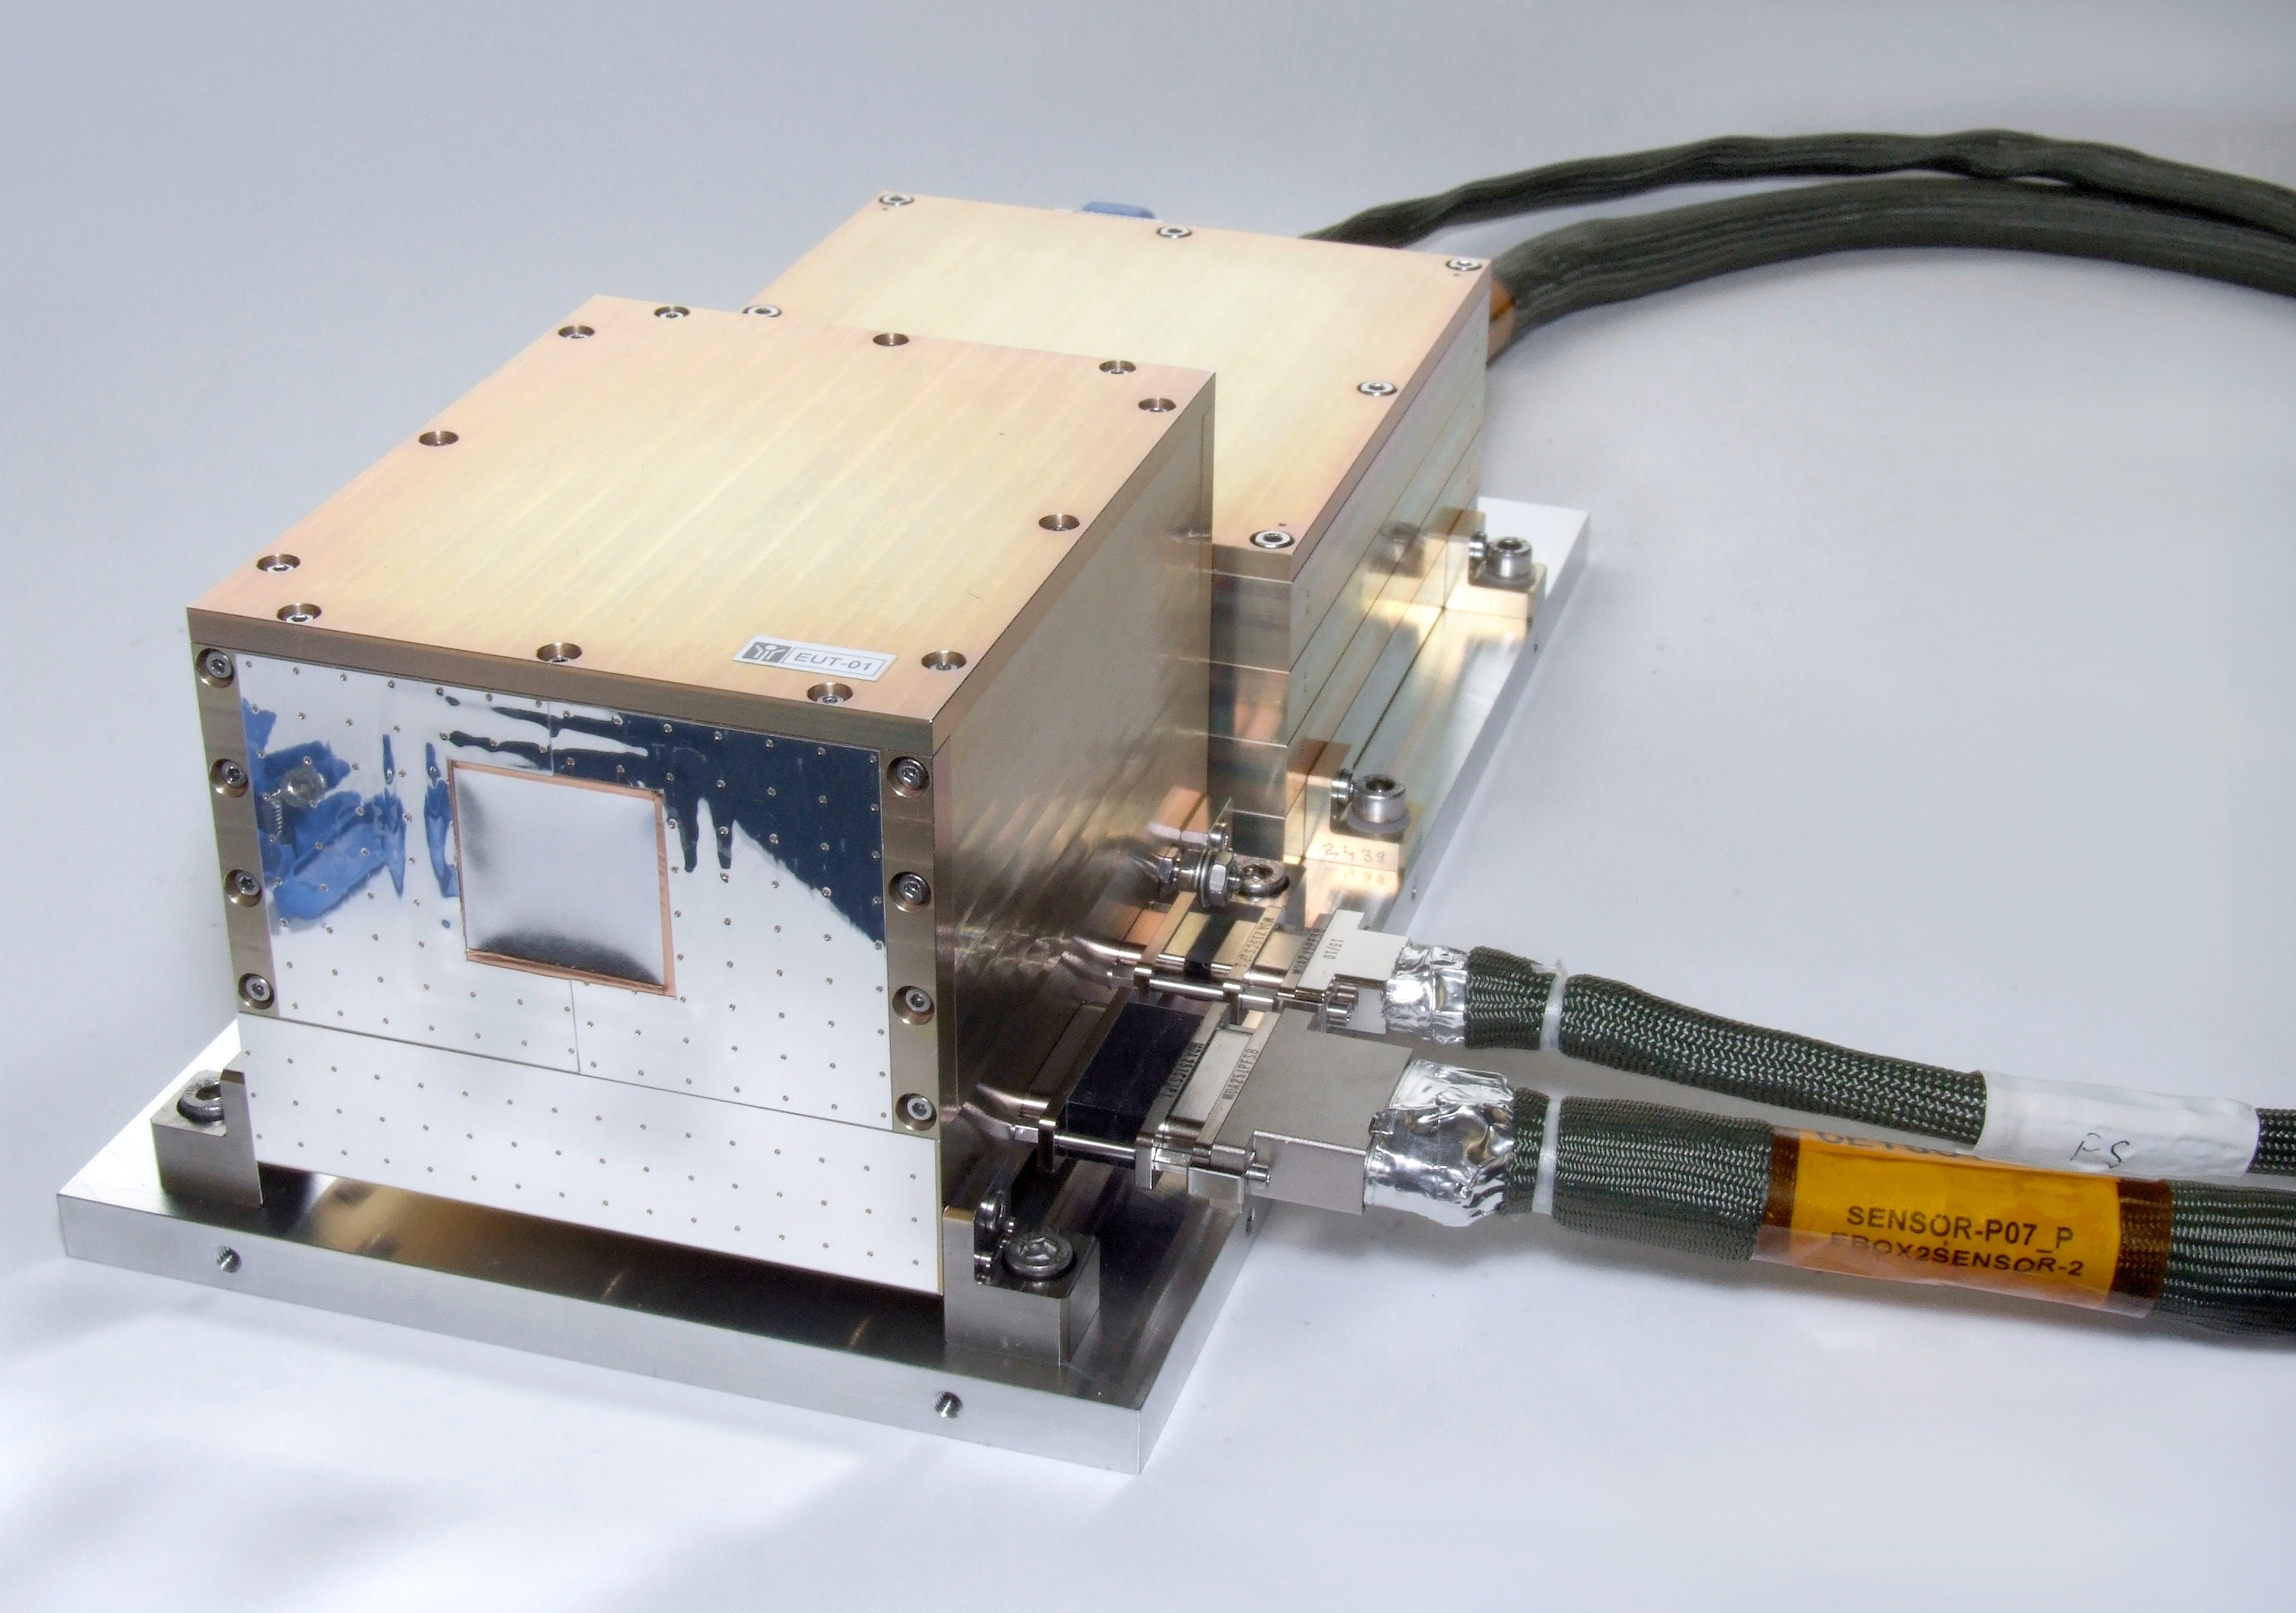
\includegraphics[width = 0.9\textwidth]{images/LND_2018-11-13.JPG}
    \caption[A Photograph of the \ac{LND}]{A photograph of the \ac{LND}, including the \ac{SH} in the front, \ac{EB} in the rear and 1-meters data and power harness that connects the \ac{SH} and \ac{EB}. The figure was adapted from \citet{Wimmer2020SSRv} and show the flight spare model of LND and was taken on 2018.11.23.}
    \label{Fig:LND_instrument}
\end{figure}


\begin{figure}[!htbp]
    \centering
    \includegraphics[width = 0.7\textwidth, height = 0.5 \textheight]{images/change4_lnd-c9_trigger-cones-colored.pdf}
    \caption[The inner structure of LND \ac{SH}]{A sketch of the inner structure of the \ac{LND} \ac{SH}. Ten 500 $\mu$m Si \acp{SSD} are assembled in order. The different colored regions indicate the \ac{FOV} of different measurement combinations. The figure was reproduced from \citet{Wimmer-2020-LND} and more details could be found in instrument paper.}
    \label{Fig:LND_sensor_head}
\end{figure}
Chang'E-4 is a robotic spacecraft mission of China exploring the lunar far-side surface, which is also the first human soft-landing missions on the lunar far-side surface \citep{Li2021SSRv}. The whole mission consists of a lander, a rover named Yutu-2 and a relay satellite named Queqiao which works in the lunar orbit and enables the communication between the lunar far-side surface and the ground. The mission was launched on December 8, 2018 and successfully landed on the Von K\`arm\`an crater near the south pole of Moon on January 3, 2019 \citep{Wu2019NatGe}. In order to cope with the significant temperature variations on the lunar surface, the rover, lander, and scientific payloads onboard enter a hibernation state during the approximately two-week-long lunar night. This mode helps to conserve energy power and to protect the detectors.  After the extended 'sleep' night, the instruments onboard are awakened by sunlight and start operating during the lunar daytime. The initial design life time of the mission was set at a minimum of one year. Obviously this target have been successfully surpassed and the scientific instruments onboard are continuing to perform impressive measurements.

As an integral part of the Chang'E-4 mission's international scientic payload, \ac{LND}\acused{LND} is designed by the Kiel University in Germany. An image of the flight spare model of \ac{LND} is displayed in Fig.~\ref{Fig:LND_instrument}. The initial design purpose of \ac{LND} is to measure the first active radiation dose rate and monitor the radiation environment caused by changed and neutral (neutrons and $\gamma$-ray) particles, as the preparation of future human exploration of the Moon and the solar system. 
Therefore, the main scientific objects of the \ac{LND}, as indicated in the instrument paper \citep{Wimmer-2020-LND}, are "Dosimetry for human exploration of the Moon" which is based on temporal variations of the dose rate and the \ac{LET} spectra, and "Contribution to the heliospheric science" which based on the measurement of charged particles.
% \begin{itemize}
%     \item \emph{Dosimetry for human exploration of the Moon}: \ac{LND} is designed to determine the temporal variations of the dose rate and the \ac{LET} spectra which will be used to derive the quality factor \textit{Q} which is a key factor to interprete the dosimetric data.
%     \item \emph{Contribution to the heliospheric science}: The particle fluxes and time series of the flux are measured on the far-side of the Moon. This unique measurement location provides valuable insights into the propagation of the particles in the heliosphere.
% \end{itemize}
Besides, \ac{LND} also has two technological demonstration objects which are "Determine the subsurface water content in the South-Pole Aitken Basin" and "Determine the FeO content in the South-Pole Aitken Basin" \citep{Wimmer-2020-LND}.

To achieve the aforementioned scientific objectives, \ac{LND} measures and provides the data products including up to 1-minute charged and neutral particle dose rate measured in Si, up to 1-minute cadence \ac{LET} spectra, 1-minute neutral particle deposition energy spectra, 10-minutes count rates of thermal neutrons and high time resolution (1-minutes, 10-minutes) charged particles flux and high energy resolution spectra including electrons and ions from proton to iron.

As of May 2023, \ac{LND} has been successfully working on the lunar far-side surface for more than 4 years, which corresponds to approximately 50 Lunar days since Jan 3, 2019. It has largely surpassed its designed lifetime.
One of the simplest way to check whether LND is working or not is to look up during the night and check the moon phase. If you can see a new moon or the moon is in the last/first quarter phase, it indicates that the moon is moving out of the earth's shadow and that the far-side surface of moon is facing the Sun, enabling the \ac{LND} work.

Based the the operations and experiment schedule established from the ground, \ac{LND} has been completely or partly (more than half a lunar day) switched off on the 6th, 44th, 45th lunar days since the start of the mission. As of the finalization of this thesis in May 2023, we have received 46 lunar days' data from January 2019 to the end of November 2022 which are stored on the servers of Kiel University. The data have officially been published in the Lunar and Planetary Data release system \footnote{\url{moon.bao.ac.cn}}, where currently the data is available until the end of December 2022. 
%you could find the data until December 2022. 
The alternative downloading options include \ac{NASA}'s Space Science Data Coordinated Archive and, \ac{ESA}'s archive ESDC (ESAC Science Data Center) which are still in building. The instrument will continue its operation on the lunar far side and we anticipate to receive can recive more intriguing data in the future with increasing solar activities.



\subsection{LND as Charged particle telescope}

\ac{LND} has a special designed sensor head that enables it to be used as a dosimeter, neutral telescope and charged particle telescope. Here, we put our focus on the charged particle telescope in this section and a brief introduction to the other two components are given in the next section for a comprehensive overview of LND's capability.

The flight spare model of \ac{LND} which is an exact replica of the flight model currently deployed on the moon is displayed in Fig.\ref{Fig:LND_instrument}. The instrument is composed of two seperate parts, the \ac{SH} in the front and the \ac{EB} at the rear. \ac{SH} and \ac{EB} are connected by a 1-meter cable which serves to provide power and transfer data. 
The \ac{SH} is comprised of ten Si \acs{SSD} of norminal 500 $\mu$m thickness. They are labeled from A to J and assembled in a charged-particle telescope configuration as illustrated in Fig.~\ref{Fig:LND_sensor_head}.

The structure of the telescope can be further divided into two parts. The upper half consists of four detectors (A, B, C, D) with A placed 80.5 mm away from B. The detector A is crucial for the function of \ac{LND} as charged particle telescope since only particles that trigger detector A will be counted. B/C/D are assembled as close in space as possible, with zero space between B and C and 0.5 mm between C and D, enabling the anti-coincidence measuremet in the inner C segement. Such a detector arrangement is similar to the Flight Radiation Environment Detector (FRED) \citep{moeller-etal-2013, moeller-etal-2013b}. The lower half consists of three detector pairs (E/F, G/H, I/J) and an Al-Gd-Al absorber. The detector pairs are closely packed together and the absorber is designed for the detection of thermal neutrons. 20 $\mu$m thick Gd foils are inserted into E/F and G/H, creating sandwich-like structures to detect thermal neutrons. This charged particle telescope is completed by the last detector pair I/J.

By measuring the energy depostion in different \acp{SSD} and using the dE/dX - E or dE/dX - dE/dX methods which depend on the primary energy of particles, LND can easily identify the energies and species of particles. 
The averaged energy loss of the charged particle along the travel path depends on the nuclear charge $Z_1$ (equal to atomic number) and the incident velocity $\nu$. 
Such a relationship could be expressed by the well-known Bethe-Bloch formula \citep{bethe-1930, bloch-1933}:

\begin{equation}
    \frac{\dd E}{\dd x} = - \frac{Z_1^2 e^4 n_e}{4 \pi \cdot \varepsilon_0^2 \beta^2 c^2 m_e} \cdot \left[ \ln\left(\frac{2 m_e  \beta^2 c^2}{{E_B}}\right) - \ln(1 - \beta^2) - \beta^2  \right], 
    \label{eq:BB}
  \end{equation}
where $c$ is the speed of light, $\beta = \nu/c$, $E_B$ is the ionization energy of the medium that particle pass, and $n_e$ is the electron density in the medium, $m_e$ is the electron mass, and constant $epsilon_0$ is the permittivity of free space. $E$ is the energy of the particle and $x$ is the travel length of the particle in the medium.

In the energy range that \ac{LND} covers, $ln(\beta^2)$ is nearly constant and slowly changes, hence the above function could be simplified as:
\begin{equation}
    E_A \propto \frac{Z_1^2 m_1}{E_{\mathrm tot}},
    \label{eq:BB2}
\end{equation}
The product of $E_A$ and $E_{tot}$ is proportional to the nuclear charge, $Z_1$ which equals to the atomic number and the mass of elements, $m_1$. These parameters depend on the particle species and allow for the determination of particle compositions. It is worth noting that \ac{LND} has the capability to discriminate between the isotopes of elements, such as helium-3 and helium-4, despite the limited resolution and larger uncertainty in the X-mas plot (Fig.~\ref{Fig:measurement_Xmas}, See Appendix \ref{chp:appendix_LND_He3_spectra})

%The nuclear charge $Z_1$ is equal to the number of protons in the nucleus, i.e. the atomic number $Z$ of the elements. Therefore, the telescope like \ac{LND} can not determine the particle charge state and we could not tell apart fully charged \ac{GCR} and singly charged \ac{ACR}. When traversing the front foil and \acp{SSD} of \ac{LND} sensor head, those partially charged particle will be ionized and stripped the electrons, becoming fully charged \citet{Swaczyna2017ApJ}.


Once the charged particle enter the sensor head of \ac{LND}, they can be further categorized into two groups: stopping particles and penetrating particles. Stopping particles have a primary energy range between $\sim$ 8 MeV/nuc and $\sim$ 35 MeV/nuc, stopping within any of the detectors B-I. Penetrating particles possess energy above this range and have the capability to penetrate through all the detectors. In Fig.~\ref{Fig:LND-Boehm-plot}, a plot generated by the large counting statistic \ac{Geant4} \citep{Agostinelli-2003} simulation illustrates how the stopping particles are seperated by using the $E_{tot} * E_A$ as the y-axis and $E_{tot} / E_A$ as the x-axis. The data points are simulated in \ac{Geant4} based on a carefully construced \ac{LND} instrument model. This model takes into account all the inner structures within the sensor head, including the \ac{PCB} next to the detector stacks and the outer shell of the sensor head. However, we must note that a completed model including the surrounding material of \ac{LND} is unavaiable since we lack the structure information of the Chang\'E-4 lander.
A screenshot of the \ac{LND} model is provided in the appendix \ref{chp:LNDsimulation}. 

Penetrating particles have a primary energy above approximately 35 MeV/nuc, and as the name suggested, can penetrate through detectors A to I and stop in J or continue to penetrate J with more energy. The majority of the penetrating particles are fully penetrating particles, which means we can not directly measure their total energy. \acp{MIP} are among the fully penetrating particles that have extremely large initial energy from hundreds MeV to GeV but only deposit a minimal amount of energy in the detector stacks.
Since the total energy of particles is unavaiable, it is not possible to create a plot similar to Fig.~\ref{Fig:LND-Boehm-plot}. Instead, we change the formula of x-axis and y-axis to $E_I/E_A$ and $dE$ respectively. The $E_I$ is the energy deposit in the last detector I. The $dE$ is the energy deposition summed from the B, C, and D.

Notably the incident direction of the particle i.e. whether they come from above or beneath the detector, could be inferred from the penetrating data. Typically, for the particle incident from above, the ratio $E_I/E_A$ tends to be larger than 1 and while for particles entering from beneath, this value tends to be less than 1. 
By analyzing the distributions and patterns in the histogram, we can identify the albedo protons from the 2-D histogram of penetrating particles, corresponding to columns 248 - 264 in the Xmas plot (Fig.~\ref{Fig:measurement_Xmas}).
The detailed understanding of the derivations and analysis of albedo protons could be inferred from Section. ~\ref{chp:LND_GCR_albedo}


\begin{figure}
    \centering
    \includegraphics[width=0.8\textwidth]{images/LND_Boehm_plot_isotropic_on_top_of_A_annotated.png}
    \caption[LND Boehm plot of stopping particles based on the simulated data]{The different particle species are well discriminated in this LND Boehm plot which is a scatter plot of the \ac{LND} simulation data generated by the \ac{Geant4} tools \citep{Agostinelli-2003}. During the simulation, an isotropic source is positioned above detector A.}
    \label{Fig:LND-Boehm-plot}
\end{figure}


\subsection{LND as dosimeter and neutral telescope}

\ac{LND} measures the \ac{TID} in the inner B segment utilizing the energy deposition and corresponding energy spectrum. The inner segment of C, which is surrouded by the B, D and C outer segment and in anti-coincidence with all other detector segments, is used to measure the neutral dose rate caused by both fast neutrons and $\gamma$-rays. The above two measurements are the primary data products of \ac{LND}. \ac{TID} and dose in C play important roles in assessing the radiation environment on the lunar surface. 

\ac{LND} employs the E/F, G/H pairs which clamp a Gd-foil, to measure the thermal neutron flux. The Gd-foil has a large cross section for thermal neutrons, resulting in an increased possibility of interaction with those neutrons. In the calibration experiment, \ac{LND} successfully measured neutrons by calculating the energy spectrum discrepancy between E (G) and F (H) for neutrons coming from the front (back) \citet{Wimmer2020SSRv}.
However, in real measurements, the quality of the thermal neutron data is unexpectedly low due to various factors. The most prominent factors is the neutron background emitted from the \ac{RTG} and the \ac{RHU}. These radioactive sources generate heat to protect the lander and payload from the frozen night. But they also contribute largerly on the neutron background \citep{Zhang2020SciAdv}. Unfortunately, the direct measurement of the radiaion sources had never been done, and only an experimental and empirical estimation of the contamination from the background on the data were conducted by \citet{Hou2020-LNDbackground}. Based on data from laboratory experiements and Monte-carlo simulations, \citet{Hou2020-LNDbackground} confirmed the non-negligible background interference and firstly estimated the dose rate background. 

Another factor that might affect the neutron measurements is the unanticipated noise increase in these detectors. Similar to the noise issue occured in other channels, channels F2, G2 and H1 have also been troubled by an increased noise level (further discussed in Section \ref{chp:LND_GCR_albedo}). The single detector counter rates increase from $10^3$ count/min to $10^6$ count/min and energy spectra of noise channels indicate that the dominant energy is below 300 keV.
The high energy noise obscure the x-ray line at 43 keV and electron lines at 71 keV, 131 keV, and 173 keV which are used to determine the thermal neutrons flux, and make it more challenging to derive the accurate thermal neutron flux of lower intensity.
Furthermore, enhanced number of noise in those thermal neutron channels cause serious dead time issues on the data product neutron dose in C. This is because neutron measurements share the same counter buffer. The dose in C is the primary objective of \ac{LND}. In order to mitigate the dead time issue, we raise the corresponding threshold of noise detectors to few hundreds keV (depending on the noise level of each detector), resulting in the loss of the thermal neutrons data.


The remain data products related to the radiation are the \ac{LET} spectra. \ac{LND} provides three types of \ac{LET} spectra including \ac{LET} $ABC\bar{I}$, $\bar{A}BIJ$ and $ABIJ$. Those \ac{LET} spectra can be used to derived the quality factor (Q), which multiplies the absorbed dose rate to obtain the dose equivalent.
Of note is that geometry factors of these \ac{LET} spectra are also affected by the configuration changes. We provide the changes of geometry factors in the appendix of chapter \ref{chp:LND_GCR_albedo}.
%More details of the data products can be found in the instrument paper \citet{Wimmer2020SSRv}.

The first scientific result of \ac{LND} regarding the radiation environment on the lunar surface are reported in \citep{Zhang-2020-LND-firstresults}. These initial findings present the \ac{TID}, neutron dose and \ac{LET} spectra of the first two lunar days. This represents the first ever dynamic measurements of the radiation variation on the lunar surface. The averaged total absorbed dose rate in silicon is about 13.59$\pm$1.01 $\mu$Gy/hour. Amongst this total dose rate, the contribution from neutral particles is estimated to be $3.10 \pm 0.43 \mu$Gy/hour. These values are consistent with the measurements from the \ac{CRaTER} on \ac{LRO}.



\subsection{Primary data products: Xmas plots}
\label{sec:xmas}

\begin{figure}
    \centering
    \includegraphics[width =0.8\textheight, height = 0.6\textheight, angle = 90]{images/xmas-2019-01-03To2022-11-29.png}
    \caption[\ac{LND} Xmas plot from measurements]{The completed Xmas plot (274 $\times$ 64) of \ac{LND} based on the measurements between 2019.1.3 and 2022.11.29. All the data products could be found in this matrix, including neutrals, \ac{LET} spectra, \ac{TID}, stopping and penetrating charged particles, including electrons, protons, helium nuclei and heavy ions. The corresponding simulation version can be found in \citep{Wimmer2020SSRv}}
    \label{Fig:measurement_Xmas}
\end{figure}

Fig.~\ref{Fig:measurement_Xmas} is the so-called "Xmas plot" \footnote{It was the front cover of the Xmas card of IEAP group in 2017. Hence we named it Xmas plot} of the \ac{LND}.The Xmas plot is an image of \ac{LND}'s memory space shaped in a 274 $\times$ 64 matrix, where each pixel in the Xmas plot servers as a counter. In principle all data products are extracted from this matrix. 
When \ac{LND} detects the deposited energy in detectors of an effective signal, the control units will calculate onboard the appropriate position in the Xmas plot and increment the corresponding counter. 

Unlike the simulated plot in \citep{Wimmer2020SSRv}, here we showcase an Xmas plot from the actual measurements between 2019.1.3 to 2022.11.29, encompassing all the data accumulated since the first lunar day observed by \ac{LND}. The green rows are the memory space that will not be transmitted to the ground, in order to save the telemetry bandwidth. 
For a more detailed explanation of the format of the Xmas plot, I recommend \citep{Wimmer2020SSRv}.

%The major different compared with the Xmas plot in \citep{Wimmer2020SSRv} is that LND measure not only the particle incident from above but also the albedo particles moving upward, while in the simulation, we did add the albedo component. It is obvious that in the penetrating panel of Xmas plot,  a higher than backgrond branch strech from middle to the left side. This branch represents the protons moving upward with enough energy fully penetrating all the detectors as well as the extra shielding from the lander structure. More details of how to derive albedo proton flux are given in Section.~\ref{sec:albedo_proton}.

\subsection{Configuration changes of LND}

It is important to highlight that several configuration changes have been implemented after \ac{LND} was delivered and launched. Those configuration changes are reflected in 14 extra commands, which are uploaded to the control unit of \ac{LND} every morning of lunar day, fixing software issues and malfunction issues. One of the software issues arises from errors in the software pipeline where the control unit use wrong channels to determine particle energies. Another one is due to the mistakes we made in simulations when designing data products, causing location of the \ac{dps} boxes shift in the X-mas plot which is a matrix storing \ac{LND} data products (See below and \citet{Wimmer-2020-LND} for more details about the X-mas plot). Neverthless, the impact of the second problem on the data products is minor. 

The significant changes of the data products are mainly caused by raising the threshold of noise channels and by removing the A2 channel in the level 3 trigger logic. A2 represents the outer segement of the front detector A (see Appendix in Sec.~\ref{chp:LND_GCR_albedo} for more details of the changes). These changes are motivated by high observed noise levels in detectors A, G, H, I and J which appeared coincidentally with the malfunction of the front lid. The front lid of \ac{LND} is a part of the lander and is designed to protect the fragile detectors inside the \ac{SH}. The lid is opened up to allow unobstructed measurements of the particles during lunar days, and is closed immediately after the instrument is switched off, protecting the detectors from the extreme temperature dercrease on the lunar surface and the lunar night. However, on the 3rd and 4th lunar day, \ac{LND} was switched off for a short period during working time but the lid was left open. Though temperature on the lunar surface increased as the Sun rose, \ac{LND} and its detectors kept losing heat. Hence the temperature of the \ac{SH} dropped drastically, resulting in irreversible deformation of carriers and the attached detectors, particularly the detectors A and I/J in the front side and the bottom side. Consequently, the lower energy noise ($\sim$ 10 - 200 keV) experienced a significant increase.

By implemmenting the aforementioned changes, we have sucessfully reduced the noise level and mitigated its impact on the primary data products such as \ac{LET} spectra. However, it is worth noting that these changes still resulted in significant consequences for several data products. For instance, we partly lose the measurement of \acp{MIP} after the increment of the threshold of I detector; the geometry factors of two \ac{LET} spectra and penetrating particle are reduced dramatically after disabling the A2 channel, which plays a key role in \ac{LND}'s measurement logic. For a better understanding of the configuration changes and their impact on the data products, please refer to the appendix of chapter \ref{chp:LND_GCR_albedo}.
The corresponding changes of the original code in the LND data processing pipeline is given in the appendix ~\ref{chp:appendix_LND_data_process_pipeline}.

\section{Solar orbiter and High energy telescope}

Successfully launched on Feb 10, 2020, \ac{SolO} mission \citep{Mueller-2020-SolO} is an international mission cooperated between \ac{ESA} and \ac{NASA} with the aim to understand the Sun and how it controls the helisphere. As indicated in the mission paper, the following scientific questions will be answered and further studied: (a). What drives the solar wind and where dose the coronal magnetic field originate from? (b). How do solar transients drive heliospheric variability? (c). How do solar eruptions produce the energetic particle radiation that fills the heliosphere? (d). How does the solar dynamo work and drive connections between the Sun and the heliosphere?

%After finishing the cuise phase which started at June 14, 2020, \ac{SolO} has been operating in the nominla mission phase since Nov 26, 2021 as scheduled.

\ac{SolO} has an elliptic helioscentric orbit with the closest perihelion of 0.29 AU (about 42$\times10^6$ km). Using several gravity assist maneuvers during the Venus flybys and the Earth flybys, the orbit of \ac{SolO} will gradually tilt away from the ecliptic plane and in the end can be 24 degrees above the Sun's equator. As of May 2023 \ac{SolO} is still following an elliptical orbit circling the sun, with a maximum solar latitude of 8.66 degrees. \ac{SolO} has finished 5 perihelions with a closest distance of 0.292 AU on Sep 3, 2022, and has started its 6th orbit, moving away the Sun. Benefiting from the unique position of \ac{SolO} during this trip, the multiple scientific instruments onboard the \ac{SolO} could further advanced our understanding of the Sun and its effects on the heliosphere.
%Three time Venus flyby happened on Dec 27, 2020,  Aug 9, 2021 and Sep 4, 2022. The Earth GAM happend on Now 27, 2021.
%The above mentioned solo tragjectory information is taken from the Solar orbiter Consolidated Report on Mission analysis \footnotes{\url{https://issues.cosmos.esa.int/solarorbiterwiki/display/SOSP/Trajectory+Overview+-+10+February+2020+Launch}}

%in the relative field for instance the questions regarding solar coronal, solar magnetic field, solar wind, \ac{SEP}.
The \ac{EPD} \citep{RodriguezPacheco-2019-EPD} is part of the scientific payload onboard \ac{SolO}, measuring energetic particles over a large scale from few kev to GeV. The spectra, composition, time variations and directional distributions could be obtained and derived.
\ac{EPD} is comprises of four different sensors, the \ac{SIS}, the \ac{STEP}, the \ac{EPT} and the \ac{HET}. 
\ac{SIS} is a time-of-flight mass spectrometer that measures ion composition from $\sim$ 0.1 - few MeV nucleon$^{-1}$. \ac{STEP} measures electrons and ions with lower energies between 4 keV and 80 keV. The special design of \ac{STEP} allows it to have high pitch-angle resolution.
\ac{EPT} and \ac{HET} share the same electronics and they are composed of two identical sensor units that are assembled perpendicularly on \ac{SolO}. This configuration enables detection of the particle incident from four different directions. \ac{EPT} is designed to measure medium-energy electrons and ions within the energy range of 25 keV to 400 keV ($\sim$ 6 MeV for protons), while \ac{HET} completes the higher energy end, measuring electrons from 300 keV to 30 MeV and ions from 6.8 Mev/nuc to $\sim$ 100 MeV/nuc in the nominal data products. Notably, the penetrating data products of \ac{HET} could extend the energy coverage of \ac{HET} up to $\sim$ GeV/nuc \citep{Elftmann-2020-PhD}.
The completed energy coverage of those four instruments for different particle species are given in Fig.~\ref{Fig:EPD-energy-coverage}.
In this section, we provide a brief introduction of \ac{HET}, which is the focus of the study in Section \ref{chp:ACR_Helium}. Further more detailed information on the other components can be found in the instrument paper \citep{RodriguezPacheco-2019-EPD} and the first years overview paper from \citet{Wimmer2021AA}.


\begin{figure}
    \centering
    \includegraphics[width = \textwidth]{images/EPD_coverage.png}
    \caption[The energy coverage of \ac{EPD} instruments]{The energy coverage of different \ac{EPD} instruments for different particle species. This figure is an updated energy coverage plot made by \citep{JohanPhd2020}, based on the similar plot from \citep{RodriguezPacheco-2019-EPD}. The HET measurements are split into stopping and penetrating parts and the later one can largely extend \ac{HET}'s capability \citep{Elftmann-2020-PhD}.}
    \label{Fig:EPD-energy-coverage}
\end{figure}  

\subsection{High energy telescope}

\begin{figure}
    \centering
    \includegraphics[width = \textwidth]{images/het.png}
    \caption[The \ac{HET} sensor head]{The cross profile of the \ac{HET} sensor head. The detector names are labeled. Figure is reproduced from \citet{RodriguezPacheco-2019-EPD}.}
    \label{fig:HET-sensor-head}
\end{figure}

\ac{HET} is a double-ended telescope. The cross profile of the \ac{HET} sensor head is depicted in Fig.~\ref{fig:HET-sensor-head}. The sensor head of \ac{HET} consists of four 300 $\mu$m silicon \ac{SSD} stacks, with two in each side (A1, B1 in the front side and A2, B2 in the back side), and a 2-cm thickness \ac{BGO} ($Bi_{4}Ge_{3}O_{12}$) scintillator which is named as detector C in the center. The sensor head setup is similar to the configuration of the \ac{RAD}, another instrument developed by Kiel Univeristy, which is currently operating on the Martion surface.  

\ac{HET} uses the $\mathrm{dE/dX - E}$ technique to discriminate different particle species of different energy. This method is the same as the measurement principle of \ac{LND} that has been well explained before. The particle species that \ac{LND} can discriminate include electrons, protons, helium nucleus, and all heavy ions such as carbon, nitrogen, oxygen, and iron.  

Once the charged particle incident and penetrate the A detector (A1 or A2), they can be split into stopping particles and penetrating particles, depending on their energy and whether they stop in detector B/C. As given in Table 22 of \citet{RodriguezPacheco-2019-EPD}, the corresponding nominal data products are ABnC, which is corresponding to particles stopping in B with energy of 6.5 - 9.5 Me/nuc, ABC which register particles stopping in C with energy range of $\sim$10 - $\sim$ 100 MeV/nuc, and penetrating detector C with energy above 100 MeV/nuc up to infinity. 

%For the penetrating particle, their primary energy can be estimated based on the energy loss on the detector and the \ac{Geant4} simulation. The aforementioned nominal data products of HET contribute to the study of \ac{SEP}, \ac{ACR} and \ac{GCR}.


In addition to the nominal charged particle data products, it is important to emphasize the significant contribution of housekeeping data in our studies.
The housekeeping data are \ac{EPD} sensor produced instrumental data. They have the highest priority for downlink to the Earth and are used to monitor the instrument status and health. Although the housekeeping data are not designed for scientific purpose, they still provide valuable insight into the instrument performance and their contributions to the scientific studies is impressive \citep{Wimmer2021AA}.


Such a housekeeping data is the single detector counter which register signals in the \ac{BGO} scintillator crystal, this is the C detector. This counter does not require any coincidence condition and respond to particles from all directions and types. The sole requirement is that the deposited energy exceeds the threshold of the C detector. Due to its larger geometry factor, this counter exhibits better counting statistics and can be used to detect small disturbance in the \ac{GCR} background. For example \citet{Forstner-2021-SolO} use this counter to study a \ac{FD} with an ampliude of 3\% when a \ac{CME} passed \ac{SolO} on 19 April 2020. In addition, \citet{Allen2021AA_venus} found an $\sim$ 5\% drop in the count rates during the first Venus flyby. This drop is due to the planet body blockage on the \ac{FOV} of \ac{HET}.

Similar to the single detector count rate, we also utilize the L2 counters named \textit{any(a1, b1)} or \textit{any(a2,b2)} to determine the periods of \acp{SEP}. The counters sum up every signal that triggers detectors A1 (A2) and B1 (B2) in the sensor head, regardless of the primary energy and the particle species. \acp{GCR} which are slowly varying are the dominant particles in the background of this counter. Therefore, a temporal increase indicates an incoming of \ac{SEP} event. These data products exhibit better counting statistics than the nominal science data products which are designed to derive the flux. Additionally, \textit{any(a1, b1)} or \textit{any(a2,b2)} are more sensitive to lower energy particles from \acp{SEP}, as they have a lower energy threshold of $\sim$ 50 keV compared to the C counter \citep{Elftmann-2020-PhD}. The counters can detect electrons and ions with energy below 1 MeV. As a result, those two counters are particularly useful in determining the start and end time of the \ac{SEP} events, no matter what particles trigger them. In Section~\ref{chp:ACR_Helium}, where we are interested in \acp{ACR}, we remove \ac{SEP} time periods determined by this method based on the \textit{any(a1,b1)} counter to enable an accurate \ac{ACR} measurement.

For more details on the inner structure and parameters of the \ac{HET}, as well as the most update status of \ac{HET}, one could refer to \citet{RodriguezPacheco-2019-EPD, Wimmer2021AA,Elftmann-2020-PhD}.



\chapter{Studies of ICME arrival times at Earth and Mars using FD data}
\label{chp:arrival_times}

\TODO{Summary of the publications}

\newpage

The following article is reproduced from \textcite{Forstner-2018} with permission from Journal of Geophysical Research: Space Physics, \copyright American Geophysical Union:\\

\pubcite{Forstner-2018}
\hfill Own contribution: 90\%

\newpage
\newcounter{includepdfpageJGREighteen}

\addtocounter{section}{1}
\setcounter{subsection}{1} 
\phantomsection
\addcontentsline{toc}{section}{\arabic{chapter}.\arabic{section} Using Forbush Decreases to Derive the Transit Time of ICMEs Propagating from 1 AU to Mars (Publication JGR--Space Physics 2018)}
%
\phantomsection
\addcontentsline{toc}{subsection}{\arabic{chapter}.\arabic{section}.\arabic{subsection} Introduction}
\label{sec:paper_forstner2018}
\includepdf[pages={1-2}, link, linkname=paper_forstner2018, scale=.95, pagecommand={\refstepcounter{includepdfpageJGREighteen}\label{paper_forstner2018.\theincludepdfpageJGREighteen}}]{publications/Forstner_et_al-2018-JGRSpace.pdf}
%
\addtocounter{subsection}{1} 
\phantomsection
\addcontentsline{toc}{subsection}{\arabic{chapter}.\arabic{section}.\arabic{subsection} Methods and Data}
\includepdf[pages={3-5}, link, linkname=paper_forstner2018, scale=.95, pagecommand={\refstepcounter{includepdfpageJGREighteen}\label{paper_forstner2018.\theincludepdfpageJGREighteen}}]{publications/Forstner_et_al-2018-JGRSpace.pdf}
%
\addtocounter{subsection}{1} 
\phantomsection
\addcontentsline{toc}{subsection}{\arabic{chapter}.\arabic{section}.\arabic{subsection} Results and Discussion}
\includepdf[pages={6-12}, link, linkname=paper_forstner2018, scale=.95, pagecommand={\refstepcounter{includepdfpageJGREighteen}\label{paper_forstner2018.\theincludepdfpageJGREighteen}}]{publications/Forstner_et_al-2018-JGRSpace.pdf}
%
\addtocounter{subsection}{1} 
\phantomsection
\addcontentsline{toc}{subsection}{\arabic{chapter}.\arabic{section}.\arabic{subsection} Conclusion}
\includepdf[pages={13}, link, linkname=paper_forstner2018, scale=.95, pagecommand={\refstepcounter{includepdfpageJGREighteen}\label{paper_forstner2018.\theincludepdfpageJGREighteen}}]{publications/Forstner_et_al-2018-JGRSpace.pdf}
%
\addtocounter{subsection}{1} 
\phantomsection
\addcontentsline{toc}{subsection}{\arabic{chapter}.\arabic{section}.\arabic{subsection} Appendix A: Cross-Correlation Analysis Plots for Each Event}
\includepdf[pages={14-16}, link, linkname=paper_forstner2018, scale=.95, pagecommand={\refstepcounter{includepdfpageJGREighteen}\label{paper_forstner2018.\theincludepdfpageJGREighteen}}]{publications/Forstner_et_al-2018-JGRSpace.pdf}
%
\addtocounter{subsection}{1} 
\phantomsection
\addcontentsline{toc}{subsection}{\arabic{chapter}.\arabic{section}.\arabic{subsection} References}
\includepdf[pages={17-18}, link, linkname=paper_forstner2018, scale=.95, pagecommand={\refstepcounter{includepdfpageJGREighteen}\label{paper_forstner2018.\theincludepdfpageJGREighteen}}]{publications/Forstner_et_al-2018-JGRSpace.pdf}

\TODO{Summary of the publication}

\newpage

The following article is reproduced from \textcite{Forstner-2019} with permission from Space 
Weather, \copyright American Geophysical Union:\\

\pubcite{Forstner-2019}
\hfill Own contribution: 90\%

\includepdf[pages=-]{publications/Forstner_et_al-2019-Space_Weather.pdf}

\section{Outlook}

\chapter{Comparing the properties of FDs at Earth and Mars}
\label{chp:fd_properties}

While in \autoref{chp:arrival_times} \acp{FD} have mainly been used to determine the arrival time of \acp{ICME} at \SI{1}{\AU} and Mars, other properties of \acp{FD} have been neglected in these studies. However, some empirical relations between different properties of a \ac{FD} at Earth as well as between the \ac{FD} and properties of the associated \ac{ICME} are known, as shown e.g. by \citet{Belov-2008-FD,Abunin-2012-FD}. For example, there is a clear correlation between the relative \ac{FD} amplitude or the maximum decrease rate (``steepness'') with the product of the maximum solar wind speed and maximum magnetic field. This parameter $v_\text{max} \cdot B_\text{max}$ can be used to describe the intensity of the disturbance in the solar wind. The correlation is shown in Figure 8 of \citet{Belov-2008-FD} and Figure 7 of \citet{Abunin-2012-FD}.
However, solar wind plasma and magnetic field measurements at Mars are only available from the \ac{MAVEN} spacecraft since 2014, and as explained in \autoref{sec:motivation}, it does not observe the upstream solar wind continuously. Consequently, the determination of maximum values for $B$ and $v$, which would be necessary for the validation of this relation at Mars, may be complicated for many events.

Instead, in this study, we focus on the correlation of two parameters of the \acp{FD} themselves: the relative amplitude and the maximum decrease rate. These parameters are already known to be correlated at Earth, as seen in Figure 7 of \citet{Belov-2008-FD} and Figure 5 of \citet{Abunin-2012-FD}. We use our catalog of \acp{FD} from \citet{Forstner-2019}, as well as the larger catalog by \citet{Papaioannou-2019-FD-Earth-Mars} to reproduce this relation at Mars. Consulting the analytical \ac{FD} models, \acs{PDB} and \acs{ForbMod}, which were introduced in \autoref{sec:forbush}, it becomes possible to interpret the difference between the two observed relations as a result of the expansion of the interplanetary structures.

The following article is reproduced from \textcite{Forstner-2020} from Journal of Geophysical Research: Space Physics, \copyright American Geophysical Union, under the Creative Commons CC-BY (\ccLogo\ccAttribution) license:\\

\noindent\pubcite{Forstner-2020}
\hfill Own contribution: 80\%

\newpage
\newcounter{includepdfpageJGRTwenty}

\addtocounter{section}{1}
\setcounter{subsection}{1} 
\phantomsection
\addcontentsline{toc}{section}{\arabic{chapter}.\arabic{section} Comparing the Properties of ICME-Induced Forbush Decreases at Earth and Mars (Publication JGR--Space Physics 2020)}
%
\phantomsection
\addcontentsline{toc}{subsection}{\arabic{chapter}.\arabic{section}.\arabic{subsection} Introduction}
\label{sec:paper_forstner2020}
\includepdf[pages={1}, link, linkname=paper_forstner2020, scale=.9, pagecommand={\refstepcounter{includepdfpageJGRTwenty}\label{paper_forstner2020.\theincludepdfpageJGRTwenty}}]{publications/Forstner_et_al-2020-JGRSpace.pdf}
%
\addtocounter{subsection}{1} 
\phantomsection
\addcontentsline{toc}{subsection}{\arabic{chapter}.\arabic{section}.\arabic{subsection} Data Sources and Catalogs}
\includepdf[pages={2-5}, link, linkname=paper_forstner2020, scale=.9, pagecommand={\refstepcounter{includepdfpageJGRTwenty}\label{paper_forstner2020.\theincludepdfpageJGRTwenty}}]{publications/Forstner_et_al-2020-JGRSpace.pdf}
%
\addtocounter{subsection}{1} 
\phantomsection
\addcontentsline{toc}{subsection}{\arabic{chapter}.\arabic{section}.\arabic{subsection} Definitions and Methodology}
\includepdf[pages={6-7}, link, linkname=paper_forstner2020, scale=.9, pagecommand={\refstepcounter{includepdfpageJGRTwenty}\label{paper_forstner2020.\theincludepdfpageJGRTwenty}}]{publications/Forstner_et_al-2020-JGRSpace.pdf}
%
\addtocounter{subsection}{1} 
\phantomsection
\addcontentsline{toc}{subsection}{\arabic{chapter}.\arabic{section}.\arabic{subsection} Results and Discussions}
\includepdf[pages={8-16}, link, linkname=paper_forstner2020, scale=.9, pagecommand={\refstepcounter{includepdfpageJGRTwenty}\label{paper_forstner2020.\theincludepdfpageJGRTwenty}}]{publications/Forstner_et_al-2020-JGRSpace.pdf}
%
\addtocounter{subsection}{1} 
\phantomsection
\addcontentsline{toc}{subsection}{\arabic{chapter}.\arabic{section}.\arabic{subsection} Conclusions and Outlook}
%
\addtocounter{subsection}{1} 
\phantomsection
\addcontentsline{toc}{subsection}{\arabic{chapter}.\arabic{section}.\arabic{subsection} Appendix A: Location of $m_{\text{max}}$ Within the ICME Substructures}
\includepdf[pages={17-18}, link, linkname=paper_forstner2020, scale=.9, pagecommand={\refstepcounter{includepdfpageJGRTwenty}\label{paper_forstner2020.\theincludepdfpageJGRTwenty}}]{publications/Forstner_et_al-2020-JGRSpace.pdf}
%
\addtocounter{subsection}{1} 
\phantomsection
\addcontentsline{toc}{subsection}{\arabic{chapter}.\arabic{section}.\arabic{subsection} References}
\includepdf[pages={19-21}, link, linkname=paper_forstner2020, scale=.9, pagecommand={\refstepcounter{includepdfpageJGRTwenty}\label{paper_forstner2020.\theincludepdfpageJGRTwenty}}]{publications/Forstner_et_al-2020-JGRSpace.pdf}

\chapter{Major Space Weather events: The events of September 2017}
\label{chp:september_event}

Between September 4 and 10, 2017, there was a sudden increase in solar activity when Active Region 12673 produced four X-class flares, including the two strongest flares of Solar Cycle 24 (X9.3 on September 6 and X8.2 on September 10).
These solar events, associated with the release of \acp{SEP} as well as the eruption of multiple fast \acp{CME}, caused a \ac{GLE} of energetic particles on the surface of Earth (\ac{GLE} \# 72 in the \ac{GLE} database at \url{https://gle.oulu.fi/}) as well as on Mars, making it the first \ac{GLE} observed simultaneously on the surface of two different planets.
The \ac{SEP} event was very widespread (Earth and Mars had a longitudinal separation of $\sim$\SI{155}{\degree} at that time) and the largest \ac{GLE} seen on the surface of Mars with \ac{MSL}/\ac{RAD} so far. At Earth, the disturbances associated with the solar events caused, e.g., a suppression of critical high frequency (HF) radio communications systems \citep{Frissell-2018,Bland-2018} as well as navigation satellite systems such as GPS \citep{Berdermann-2018,Sato-2019}.
These major events have been studied in great detail, many of the articles concerning these events can be found in the special issues of \citet{SpaceWeather-2018-special-issue-September-event} as well as \citet{GRL-2018-special-issue-September-event}, where the latter is focusing on its impact on Mars.

While the September 6 flare had the stronger X-ray emission, the \acp{SEP} associated with the later September 10 flare is the one that caused the \ac{GLE} seen at Earth and Mars, due to the better magnetic connection. Three CMEs also erupted on September 9 and 10 from the same active region in similar directions ($\sim$\SI{115}{\degree} in \ac{HEE} coordinates), the last one with an extremely high speed of more than \SI{2600}{\kilo\meter\per\second}. This fast and wide CME quickly merged with the two previous ones and formed an intense interplanetary shock, propagated outward and was observed \textit{in situ} at both Earth and Mars on September 12 and 13, respectively. While the \ac{SEP} event at Mars was still in its declining phase, the shock arrival caused an intense \ac{FD} at Mars with an amplitude of \SI{15}{\percent}, the largest \ac{FD} seen by \ac{RAD} to date. This decrease below the pre-\ac{SEP} levels was sustained over 5 days and then gradually recovered over the course of several weeks.

The following two articles \citep{Zeitlin-2018,Guo-2018} study the effects of the September 10 events on Mars as measured by \ac{MSL}/\ac{RAD} and explain these observations by modeling the \ac{SEP} event and the three \acp{CME}. \citet{Zeitlin-2018} report the dosimetric quantities on the Martian surface, emphasizing that the increased dose and dose equivalent rates during the \ac{GLE} on Mars are almost canceled out by the long-lasting \ac{FD} following it. Thus, in the case of a long-stay mission scenario, the increased radiation exposure due to the September event would have been insignificant for astronauts on Mars despite the 2- to 3-fold increase during the peak of the \ac{SEP} event. However, as Mars was not particularly well connected to the active region, the impact of the \ac{SEP} event could have been much larger, so this conclusion should not be generalized to all major solar events at Mars. In \citet{Guo-2018}, the propagation of the 3 \acp{ICME} towards Earth and Mars is studied in more detail. The initial parameters of the \acp{CME} close to the Sun are reconstructed using \ac{GCS} fitting, and then the kinematics of the propagation are calculated using the empirical \ac{DBM} \citep{Vrsnak-2007,Vrsnak-2013}. This is one of the first instances where \ac{DBM} is used to predict the merging of multiple \acp{ICME} --- for this process, a simple conservation of momentum is assumed, and with a sensible choice of the drag parameter $\gamma$, it fits the observed arrival times at Earth and Mars. The results are also compared to more sophisticated \ac{MHD} simulations performed for the same event.

\newpage

The following article is reproduced from \textcite{Zeitlin-2018} with permission from Geophysical Research Letters, \copyright American Geophysical Union:\\

\noindent
\pubcite{Zeitlin-2018}
\hfill Own contribution: 10\%

\newpage
\newcounter{includepdfpageZeitlinEighteen}

\addtocounter{section}{1}
\setcounter{subsection}{1} 
\phantomsection
\addcontentsline{toc}{section}{\arabic{chapter}.\arabic{section} Analysis of the radiation hazard observed by RAD on the surface of Mars during the September 2017 solar particle event (Publication GRL 2018)}
%
\phantomsection
\addcontentsline{toc}{subsection}{\arabic{chapter}.\arabic{section}.\arabic{subsection} Introduction}
\label{sec:paper_zeitlin2018}
%
\addtocounter{subsection}{1} 
\phantomsection
\addcontentsline{toc}{subsection}{\arabic{chapter}.\arabic{section}.\arabic{subsection} Triggering and Data Acquisition}
%
\includepdf[pages={1}, link, linkname=paper_zeitlin2018, scale=.95, pagecommand={\refstepcounter{includepdfpageZeitlinEighteen}\label{paper_zeitlin2018.\theincludepdfpageZeitlinEighteen}}]{publications/Zeitlin_et_al-2018-Geophysical_Research_Letters}
%
\addtocounter{subsection}{1} 
\phantomsection
\addcontentsline{toc}{subsection}{\arabic{chapter}.\arabic{section}.\arabic{subsection} Results}
\includepdf[pages={2-5}, link, linkname=paper_zeitlin2018, scale=.95, pagecommand={\refstepcounter{includepdfpageZeitlinEighteen}\label{paper_zeitlin2018.\theincludepdfpageZeitlinEighteen}}]{publications/Zeitlin_et_al-2018-Geophysical_Research_Letters}
%
\addtocounter{subsection}{1} 
\phantomsection
\addcontentsline{toc}{subsection}{\arabic{chapter}.\arabic{section}.\arabic{subsection} Conclusions}
\includepdf[pages={6}, link, linkname=paper_zeitlin2018, scale=.95, pagecommand={\refstepcounter{includepdfpageZeitlinEighteen}\label{paper_zeitlin2018.\theincludepdfpageZeitlinEighteen}}]{publications/Zeitlin_et_al-2018-Geophysical_Research_Letters}
%
\addtocounter{subsection}{1} 
\phantomsection
\addcontentsline{toc}{subsection}{\arabic{chapter}.\arabic{section}.\arabic{subsection} References}
\includepdf[pages={7}, link, linkname=paper_zeitlin2018, scale=.95, pagecommand={\refstepcounter{includepdfpageZeitlinEighteen}\label{paper_zeitlin2018.\theincludepdfpageZeitlinEighteen}}]{publications/Zeitlin_et_al-2018-Geophysical_Research_Letters}
\newpage

The following article is reproduced from \textcite{Zeitlin-2018} with permission from Geophysical Research Letters, \copyright American Geophysical Union:\\

\pubcite{Guo-2018}
\hfill Own contribution: 10\%

\newpage
\newcounter{includepdfpageGuoEighteen}

\addtocounter{section}{1}
\setcounter{subsection}{1} 
\phantomsection
\addcontentsline{toc}{section}{\arabic{chapter}.\arabic{section} Modeling the Evolution and Propagation of 10 September 2017 CMEs and SEPs Arriving at Mars Constrained by Remote Sensing and In Situ Measurement (Publication Space Weather 2018)}
%
\includepdf[pages={1}, link, linkname=paper_guo2018, scale=.95, pagecommand={\refstepcounter{includepdfpageGuoEighteen}\label{paper_guo2018.\theincludepdfpageGuoEighteen}}]{publications/Guo_et_al-2018-Space_Weather}
%
\phantomsection
\addcontentsline{toc}{subsection}{\arabic{chapter}.\arabic{section}.\arabic{subsection} The Flare, CMEs, and GLE 72: Close to the Sun}
\label{sec:paper_guo2018}
%
\includepdf[pages={2-4}, link, linkname=paper_guo2018, scale=.95, pagecommand={\refstepcounter{includepdfpageGuoEighteen}\label{paper_guo2018.\theincludepdfpageGuoEighteen}}]{publications/Guo_et_al-2018-Space_Weather}
%
\addtocounter{subsection}{1} 
\phantomsection
\addcontentsline{toc}{subsection}{\arabic{chapter}.\arabic{section}.\arabic{subsection} The Interplanetary Trajectory and Interaction of Three CMEs Modeled by the DBM}
\includepdf[pages={5-6}, link, linkname=paper_guo2018, scale=.95, pagecommand={\refstepcounter{includepdfpageGuoEighteen}\label{paper_guo2018.\theincludepdfpageGuoEighteen}}]{publications/Guo_et_al-2018-Space_Weather}
%
\addtocounter{subsection}{1} 
\phantomsection
\addcontentsline{toc}{subsection}{\arabic{chapter}.\arabic{section}.\arabic{subsection} Shock Kinematics and Propagation Toward Earth and Mars: Data-Constrained DBM}
\includepdf[pages={7}, link, linkname=paper_guo2018, scale=.95, pagecommand={\refstepcounter{includepdfpageGuoEighteen}\label{paper_guo2018.\theincludepdfpageGuoEighteen}}]{publications/Guo_et_al-2018-Space_Weather}
%
\addtocounter{subsection}{1} 
\phantomsection
\addcontentsline{toc}{subsection}{\arabic{chapter}.\arabic{section}.\arabic{subsection} The Shock and ICME Arrival at Mars and Earth: Modeled Results and In Situ Observations}
\includepdf[pages={8}, link, linkname=paper_guo2018, scale=.95, pagecommand={\refstepcounter{includepdfpageGuoEighteen}\label{paper_guo2018.\theincludepdfpageGuoEighteen}}]{publications/Guo_et_al-2018-Space_Weather}
%
\addtocounter{subsection}{1} 
\phantomsection
\addcontentsline{toc}{subsection}{\arabic{chapter}.\arabic{section}.\arabic{subsection} SEPs Arriving at Earth, Mars, and STA and the Indication of the Shockand Stream Interaction Region Propagation}
\includepdf[pages={9-10}, link, linkname=paper_guo2018, scale=.95, pagecommand={\refstepcounter{includepdfpageGuoEighteen}\label{paper_guo2018.\theincludepdfpageGuoEighteen}}]{publications/Guo_et_al-2018-Space_Weather}
%
\addtocounter{subsection}{1} 
\phantomsection
\addcontentsline{toc}{subsection}{\arabic{chapter}.\arabic{section}.\arabic{subsection} Summary and Conclusion}
\includepdf[pages={11}, link, linkname=paper_guo2018, scale=.95, pagecommand={\refstepcounter{includepdfpageGuoEighteen}\label{paper_guo2018.\theincludepdfpageGuoEighteen}}]{publications/Guo_et_al-2018-Space_Weather}
%
\addtocounter{subsection}{1} 
\phantomsection
\addcontentsline{toc}{subsection}{\arabic{chapter}.\arabic{section}.\arabic{subsection} Appendix A: References of the Measurements and Databases Employed in This Study}
\includepdf[pages={12}, link, linkname=paper_guo2018, scale=.95, pagecommand={\refstepcounter{includepdfpageGuoEighteen}\label{paper_guo2018.\theincludepdfpageGuoEighteen}}]{publications/Guo_et_al-2018-Space_Weather}
%
\addtocounter{subsection}{1} 
\phantomsection
\addcontentsline{toc}{subsection}{\arabic{chapter}.\arabic{section}.\arabic{subsection} References}
\includepdf[pages={13-14}, link, linkname=paper_guo2018, scale=.95, pagecommand={\refstepcounter{includepdfpageGuoEighteen}\label{paper_guo2018.\theincludepdfpageGuoEighteen}}]{publications/Guo_et_al-2018-Space_Weather}

\chapter{Case study: First CME seen at Solar Orbiter}
\label{chp:solo}

Together with the NASA \ac{PSP} launched in August 2018, the ESA \ac{SolO} mission ushers in a new era of solar and heliospheric physics. For the first time since the 1970s, these spacecraft will approach the Sun significantly closer than the orbit of Mercury --- \ac{PSP} has already set a new record with less than \SI{0.1}{\AU} solar distance at its most recent perihelion in September 2020. On the other hand, \ac{SolO}, which was launched in February 2020, will come very close to the Sun as well ($\sim\SI{0.28}{\AU}$), although it will stay far enough away to also allow for imaging observations through holes in its heatshield. In the extended mission phase, it is planned to incline the orbit of \ac{SolO} to also observe the poles of the Sun directly for the first time.

As part of the \ac{EPD} suite on \ac{SolO} \citep{RodriguezPacheco-2019-EPD}, the \acl{HET}\acused{HET} (\acs{HET}, \autoref{sec:solohet}) has been successfully commissioned and is providing some first measurements of high-energy charged particles. While a few \ac{SEP} events in the first 10 months of the mission did extend to the energies covered by \ac{HET} ($\gtrsim\SI{6}{\mega\electronvolt\per nuc}$ ions and $>\SI{450}{\kilo\electronvolt}$ electrons), \ac{HET} spent most of the time observing the \ac{GCR} background, as the solar activity was quite low during this time. As discussed in \autoref{sec:solohet}, \ac{HET} is also able to resolve short-term variations of \acp{GCR} with some of its data products. Consequently, some \acp{FD} could be measured, which were caused by \acp{CME} and \acp{CIR} that passed \ac{SolO} during its first orbit.

The first \ac{CME}-induced \ac{FD} seen at \ac{SolO} on April 19, 2020 is especially interesting, as it is a multispacecraft event that was also observed near Earth one day later during a close longitudinal alignment and with a radial separation of \SI{0.2}{\AU}. Measurements of the \ac{FD} near Earth have been taken by neutron monitors as well as the \ac{CRaTER} onboard the \ac{LRO}. The \ac{CME} was also seen at the BepiColombo spacecraft that was still close to Earth at this time, and may also have hit Venus, though no observations are available at this location due to the loss of contact with the Venus Express spacecraft since 2014. Furthermore, \acs{STEREO}-A was in an excellent position to provide a side view of the \ac{CME} with its remote sensing instruments. In the following publication, which was submitted to \textit{Astronomy \& Astrophysics} in November 2020, we describe the capabilities of \ac{HET}, present the \ac{FD} observed at \ac{SolO} and the corresponding observations near Earth, and investigate the radial evolution of the \ac{CME} by applying \acs{ForbMod} (see \autoref{sec:forbush}) to this event. Two other studies of the same event, have also been submitted to \textit{A\&A}: \textcite{Davies-2021} focus on the magnetic field observations, while \textcite{OKane-2021-SolO} investigate the solar source of the CME. All three papers will be published in the \textit{A\&A} ``Solar Orbiter First Results'' special issue in 2021.

In the process of this study, a new software implementation of the \ac{GCS} model \citep{Thernisien-2011-GCS} has been developed. Details about this tool can be found in \autoref{chp:GCS_Python}.

\newpage

The following article is reproduced from \textcite{Forstner-2020-SolO} with permission from Astronomy \& Astrophysics, \copyright The European Southern Observatory (ESO):\\

\pubcite{Forstner-2020-SolO}
\hfill Own contribution: 80\%

\newpage
\newcounter{includepdfpageAATwenty}

\todo[inline]{Insert Article}


% ********************************************************************
% Backmatter
%*******************************************************
\newpage
\markboth{}{\thepage}
\cleardoublepage
\phantomsection
\addcontentsline{toc}{chapter}{Bibliography}

\printbibliography

\cleardoublepage
%*******************************************************
% Acknowledgements
%*******************************************************
\refstepcounter{dummy}
\pdfbookmark[0]{Acknowledgements}{Acknowledgements}
\chapter*{Acknowledgements}




At this point, I would like to thank everyone who supported me during the course of my PhD studies and my work on MSL/RAD, Chang'E 4 LND as well as Solar Orbiter EPD.

First of all, I am grateful to my supervisor Prof. Robert Wimmer-Schweingruber for the opportunity to work on these exciting projects, and his helpful advice. He also made it possible that these results could be published in scientific journals and presented at many international conferences. Sincere thanks also to Prof. Jingnan Guo, who supported my work since my bachelor's thesis, and who I wish all the best for her new position in China.

Furthermore, thanks to all my colleagues in the three mission teams for their continued support and helpful discussions, including Zigong Xu, Alexander Kollhoff, and my officemate Christoph Terasa for the productive and enjoyable collaboration, e.g. on low- and high-level software for the Solar Orbiter mission, which will hopefully facilitate the EPD data analysis in the Kiel team for years to come, and to the rest of the Extraterrestrial Physics group at Kiel University. I also thank the group of Manuela Temmer and Astrid Veronig at the University of Graz and Mateja Dumbović at Hvar Observatory with whom I worked in close collaboration for many of the Forbush decrease studies, and who I enjoyed meeting regularly at the conferences in Vienna, Hvar and San Francisco.

I additionally want to thank the bachelor and master students who supported my work during their Hiwi positions, Charlotte Büschel and Niklas Lundt, and three secondary school students, Joana Wanger, Lukas Abegg and Markus Arndt, who contributed to the data sets used in my studies during their internships in the ET group.

I would like to thank Anne Fischer as well as Hanna Giese and Knud Schröter for their very thorough proofreading of this thesis and valuable suggestions, and my parents Kristina and Michael and my brother Julius for their moral support. 

Last but not least, the data analysis presented in this thesis, the typesetting of the thesis itself and the generation of most of the figures were made possible by a number of open source software projects, including, but not limited to, the ones acknowledged below:

\begin{refsection}[software.bib]
	\nocite{*}
	\newrefcontext[sorting=none]
	\printbibliography[heading=none]
\end{refsection}

\cleardoublepage
\appendix
\chapter{Isotropic simulation of the High Energy Telescope with the Solar Orbiter spacecraft model}
\label{chp:HETSimulation}

To simulate the response of the \acl{HET} (\acs{HET}, \autoref{sec:solohet}), part of the \acl{EPD} \citep[\acs{EPD},][]{RodriguezPacheco-2019-EPD} onboard \ac{SolO}, for an isotropic radiation field, a simulation using the \acl{Geant4} toolkit \citep[\acs{Geant4},][]{Agostinelli-2003} was performed. GEANT4 is a software toolkit developed at CERN for Monte Carlo simulations of the interaction of particles with matter, and is widely used in many different fields. A \ac{Geant4} simulation typically requires the definition of a particle source (e.g. a particle beam, a surface or volume source), a model of the geometry and materials of the experimental setup, and one or more sensitive detectors in which particle hits are detected. A so-called ``physics list'' describes all possible interaction processes and their probabilities, from which \ac{Geant4} then chooses stochastically for each simulated particle. As a result, the trajectory of each particle and the detected particles in each detector can be stored and used processed to calculate e.g. the response function of a particle detector.

This simulation builds on top of the work by \citet{Elftmann-2020-PhD}, who simulated the nominal data products of \ac{HET} with \ac{Geant4}. In this case, particles were simulated only from a circular source in front of the A detector \citet[Figure 5.1]{Elftmann-2020-PhD}, which fills the nominal \ac{FOV} of \ac{HET}. However, particles entering \ac{HET} from outside its \ac{FOV} may also play a role for certain data products, especially for single-detector counters, which are sensitive to particles entering the telescope from all directions (e.g., through the housing). These counters were used by \citet{Forstner-2021-SolO} to observe Forbush decreases with \ac{HET}. Thus, it makes sense to simulate the \ac{HET} detector in an isotropic particle flux to model its response to \acp{GCR}, and this will be done in \autoref{sec:isotropic_sim}.

For an isotropic particle flux, it is also important to take into account the Solar Orbiter spacecraft that \ac{HET} is mounted on. This is less relevant for the nominal \ac{FOV}, as the \ac{HET} telescopes are oriented so that their openings do not point towards the spacecraft body (i.e. tangential to an edge of the body). But for single detector counters, particles coming from the solid angle covered by the spacecraft can be shielded away, or may generate secondaries that are then detected within \ac{HET}. This will be investigated in \autoref{sec:spacecraft_model}.

\section{Isotropic simulation of HET}
\label{sec:isotropic_sim}

For the isotropic simulation, the geometric model of the \ac{HET} instrument and its electronics box were reused from the simulation by \citet{Elftmann-2020-PhD}, so the reader is referred to this work for further details about its definition. The simulation setup was also very similar to \citet{Elftmann-2020-PhD}, using \ac{Geant4} version 10.1.2 with the pre-defined general-purpose physics list \texttt{QGSP\_BERT}, and a power law spectrum for the energy-dependent intensity $I$ of the input particles:
\begin{equation}
I(E) \sim E^{-1}
\label{eq:het_g4_spectrum}
\end{equation}
This makes it possible to simulate the same number of particles in each primary energy bin when the bins are logarithmically spaced. Only protons between \SI{5}{\mega\electronvolt} and \SI{100}{\giga\electronvolt} were simulated as input particles in this case, as other species were neglected in the modeling approach of \citet{Forstner-2021-SolO}. Still, all secondary particles generated by these primary protons are taken into account in the output of simulation. Of course, other primary species such as electrons and heavy ions can be simulated in a similar fashion in the future, though in this case, the quenching model needs to be taken into account, as described by \citet[Section 5.4]{Elftmann-2020-PhD} and \citet{Tammen-2015}.

In contrast to the circular planar source surface used by \citet{Elftmann-2020-PhD}, a spherical source with a radius of \SI{15}{\centi\meter} (large enough to surround \ac{HET} and its electronics box) was defined, and particles were injected following a cosine-law angular distribution. This represents an isotropic flux entering \ac{HET} from all sides.
The simulation was run for $N_\text{total} = \num{5e8}$ particles, and $\sim\num{1.6e7}$ particle hits (primary or secondary) were registered in the \ac{HET} detectors (ratio: \SI{3.2}{\percent}).

\section{The spacecraft model}
\label{sec:spacecraft_model}

To simulate how the interaction of \ac{GCR} particles with the Solar Orbiter spacecraft affects the \ac{HET} measurements, the spacecraft needs to be included into the \ac{Geant4} simulation. Accurately modeling a spacecraft is notoriously difficult, as it consists of numerous components and information about their exact shape and composition is not always readily available. Thus, simulations taking into account spacecraft effects often need to make many assumptions and drastically simplify the geometry of the spacecraft (see e.g. \citet{Appel-2018-PhD,Appel-2018} for a similar simulation of the Mars Science Laboratory rover).

In the case of Solar Orbiter, ESA has provided a computer-aided design (CAD) model of the spacecraft that can serve as a reference for simulations (D. Müller, 2020, priv. comm.). This file (\texttt{dpl7a1\_bulk.bdf}) is provided in the NASTRAN BDF format
and contains the 3D geometry of the spacecraft, including material properties such as the density. Using the freeware software \textit{FEX}\footnote{\url{http://www.f-e-x.com/}}, it is possible to inspect the model and measure the dimensions and total mass of certain structures.

As shown in \autoref{fig:solo_spacecraft_model}, the model accurately represents the major structures of the SolO spacecraft, such as the main body, the solar panels, the heat shield, the instrument boom and various communications and radio wave antennae. However, not all parts are modeled in detail: Many small structures, such as the scientific payload and electronics within the spacecraft body, are replaced with mass points that are attached to the model (shown as colored tetrahedra in the image), and thus no information about their extent and materials are provided. In addition, some parts of the spacecraft are constructed using composite materials, such as honeycomb structures instead of solid Aluminium --- in these cases, the material properties given in the CAD file do not include the correct density, but are instead set to zero. Thus, the total mass of the spacecraft according to the CAD file is \SI{1202}{\kilogram}, which is significantly less than the total launch mass off $\sim\SI{1800}{\kilo\gram}$, or $\sim\SI{1600}{\kilo\gram}$ without fuel \citep{Mueller-2020-SolO}.

\begin{figure}
	\centering
	\includegraphics[width=0.7\linewidth]{images/solo_spacecraft_model}
	\caption[Density model of the Solar Orbiter spacecraft]{Density model of the Solar Orbiter spacecraft as supplied by ESA. Colored tetrahedra correspond to mass points that are inserted into the model as a replacement for structures whose geometry is not modeled (e.g. scientific payload).}
	\label{fig:solo_spacecraft_model}
\end{figure}

An automated conversion from the CAD file to a \ac{Geant4}-compatible model (GDML) is not easily possible and would also not be very meaningful due to the shortcomings of the CAD model described above.
As a first step towards implementing the spacecraft model in \ac{Geant4}, I have therefore simply measured the dimensions of the main box-shaped spacecraft body in the CAD file and created a corresponding box in \ac{Geant4}. To estimate the mass of this box, the following estimations are made: 
The total mass of the two solar panels in the CAD file is \SI{110}{\kilo\gram}, so the main spacecraft body (without solar panels) has a mass of $\sim\SI{1100}{\kilogram} + \SI{600}{\kilogram} = \SI{1700}{\kilogram}$ (adding the \SI{400}{\kilogram} of mass that is ``missing'' in the CAD file \SI{200}{\kilogram} of fuel). This value is used as the mass of the box in the \ac{Geant4} model.
For the material of the box, we assume that the mass is equally distributed throughout the box, with \SI{200}{\kilogram} of hydrazine fuel, and the remaining mass split 50:50 between electronics components and aluminium (\SI{750}{\kilogram} each). Electronics were modeled using the \ac{PCB} material taken from \citet{Appel-2018,Appel-2018-PhD}.
The dimensions and materials used are summarized in \autoref{tab:solo_spacecraft_gdml}.

\begin{table}
    \begin{tabular}{rp{6cm}}
        \toprule
        \multicolumn{2}{c}{\textbf{SolO spacecraft body}}                   \\
        \midrule
        X dimension & \SI{1812}{\milli\meter}                \\
        Y dimension & \SI{1461}{\milli\meter}                \\
        Z dimension & \SI{2200}{\milli\meter}                \\
        Mass        & \SI{1700}{\kilogram}                   \\
        Density     & \SI{291.89}{\kilogram\per\cubic\meter} \\
        Composition & \SI{12}{\percent} Hydrazine (N$_2$H$_4$) \newline \SI{44}{\percent} \ac{PCB} material (see right table) \newline \SI{44}{\percent} Aluminium Alloy (same as \ac{HET} housing) \\
        \bottomrule
    \end{tabular}
    \hspace{1cm}
    \begin{tabular}{rr}
    	\toprule
    	\multicolumn{2}{c}{\textbf{\ac{PCB} material}} \\ \midrule
    	Cu      & \SI{20}{\percent}     \\
    	SiO$_2$ & \SI{15}{\percent}     \\
    	PET     & \SI{9.9}{\percent}    \\
    	PP      & \SI{4.8}{\percent}    \\
    	Al      & \SI{2}{\percent}      \\
    	Pb      & \SI{2}{\percent}      \\
    	Ni      & \SI{2}{\percent}      \\
    	Fe      & \SI{8}{\percent}      \\
    	Sn      & \SI{4}{\percent}      \\
    	Mg      & \SI{30}{\percent}     \\ \bottomrule
    \end{tabular}
    \caption{Details of the spacecraft model used for the \ac{HET} simulation. The left table shows the dimensions and composition of the box-shaped spacecraft body, while the right table shows the \ac{PCB} material taken from \citet{Appel-2018,Appel-2018-PhD}.}
    \label{tab:solo_spacecraft_gdml}
\end{table}

\ac{HET} was then positioned next to the spacecraft body, at a location derived from the position of the corresponding mass point of \ac{HET} 1 in the CAD file, and with the correct orientation relative to the Sun. As both \ac{HET} 1 and \ac{HET} 2 are located at an edge of the spacecraft body, the difference between the positions of \ac{HET} 1 and \ac{HET} 2 is not expected to be significant for an isotropic radiation field --- but of course, this may be verified with another simulation in the future. As a source, a cube of edge length \SI{260}{\centi\meter}, which surrounds the spacecraft body and the \ac{HET} sensor was used, again with a cosine-law distribution of particles injected from its surface. Due to the large source size, the simulation needed to be run multiple times with different random seed values to generate a sufficient amount of statistics. In total, $N_\text{total} = \num{1.6e10}$ primary particles were simulated, resulting in \num{5.6e6} hits in the \ac{HET} detectors (ratio: \SI{0.035}{\percent}).

To speed up future simulations, the spacecraft model may also be converted into spherical shells of equivalent column density that are placed around the \ac{HET} sensor. In this case, the source size could be significantly reduced and thus the fraction of simulated particles that reach \ac{HET} would increase. The simulation results with the actual spacecraft geometry can then be used to validate this approach.

\section{Analysis of the simulation results}

For the study presented in \citet{Forstner-2021-SolO}, the data analysis applied to the simulation results was fairly simple. To calculate the response function of the \ac{HET} C detector single counters, the detected events were first filtered for hits in the C detector (detector ID 6 in the \ac{Geant4} simulation), which deposited more than a certain threshold energy $E_\text{th}$ in this detector. The C detector single counters have threshold energies of \SI{4}{\mega\electronvolt} for the low-gain channel and \SI{10}{\mega\electronvolt} for the high-gain channel, so the analysis was run for both of these values.

Next, the primary energy of the particles corresponding to these events was taken to calculate a histogram with $k=200$ logarithmically-spaced bins spanning the whole primary energy range. To calculate the energy-dependent geometric factor $G$ for each primary energy from this histogram, the following formula \citep[based on][equation 18]{Sullivan-1971} was used:
\begin{equation}
G(E) = \frac{n(E)}{N(E)} \cdot G_\text{source}
\end{equation}
where $n(E)$ is the number of hits in the C detector for primary particles of energy $E$, $N(E)$ is the number of primary particles simulated at this energy, and
\begin{equation}
G_\text{source} = \pi A_\text{source}
\end{equation}
\citep[equation 6]{Sullivan-1971} is the geometric factor of the particle source, which is calculated from the surface area of the spherical or cubical particle source. $N(E)$ is easy to calculate due to the chosen input spectrum (\autoref{eq:het_g4_spectrum}), which results in the same number of particles in each of the $k$ energy bins, i.e.
\begin{equation}
N(E) = \frac{N_\text{total}}{k}
\end{equation}
The resulting response function $G(E)$ is plotted in \autoref{fig:het_c_responsefunction}. As explained by \citet[Section 2.1]{Forstner-2021-SolO}, the narrow plateau below $\sim\SI{20}{\mega\electronvolt}$ corresponds to particles entering through the nominal field of view (i.e. through the A and B detectors), while the following increase is caused by particles that penetrate the \ac{HET} housing. The effect of the spacecraft model on the response is as expected: A slight decrease for lower energies up to $\sim\SI{200}{\mega\electronvolt}$ due to shielding, and a significant increase for high energies above $\SI{1}{\giga\electronvolt}$ due to the generation of secondaries in the spacecraft body.

\begin{figure}
	\centering
	%% Creator: Matplotlib, PGF backend
%%
%% To include the figure in your LaTeX document, write
%%   \input{<filename>.pgf}
%%
%% Make sure the required packages are loaded in your preamble
%%   \usepackage{pgf}
%%
%% and, on pdftex
%%   \usepackage[utf8]{inputenc}\DeclareUnicodeCharacter{2212}{-}
%%
%% or, on luatex and xetex
%%   \usepackage{unicode-math}
%%
%% Figures using additional raster images can only be included by \input if
%% they are in the same directory as the main LaTeX file. For loading figures
%% from other directories you can use the `import` package
%%   \usepackage{import}
%%
%% and then include the figures with
%%   \import{<path to file>}{<filename>.pgf}
%%
%% Matplotlib used the following preamble
%%   \usepackage{fontspec}
%%   
%%
\begingroup%
\makeatletter%
\begin{pgfpicture}%
\pgfpathrectangle{\pgfpointorigin}{\pgfqpoint{5.000000in}{3.300000in}}%
\pgfusepath{use as bounding box, clip}%
\begin{pgfscope}%
\pgfsetbuttcap%
\pgfsetmiterjoin%
\definecolor{currentfill}{rgb}{1.000000,1.000000,1.000000}%
\pgfsetfillcolor{currentfill}%
\pgfsetlinewidth{0.000000pt}%
\definecolor{currentstroke}{rgb}{1.000000,1.000000,1.000000}%
\pgfsetstrokecolor{currentstroke}%
\pgfsetdash{}{0pt}%
\pgfpathmoveto{\pgfqpoint{0.000000in}{0.000000in}}%
\pgfpathlineto{\pgfqpoint{5.000000in}{0.000000in}}%
\pgfpathlineto{\pgfqpoint{5.000000in}{3.300000in}}%
\pgfpathlineto{\pgfqpoint{0.000000in}{3.300000in}}%
\pgfpathclose%
\pgfusepath{fill}%
\end{pgfscope}%
\begin{pgfscope}%
\pgfsetbuttcap%
\pgfsetmiterjoin%
\definecolor{currentfill}{rgb}{1.000000,1.000000,1.000000}%
\pgfsetfillcolor{currentfill}%
\pgfsetlinewidth{0.000000pt}%
\definecolor{currentstroke}{rgb}{0.000000,0.000000,0.000000}%
\pgfsetstrokecolor{currentstroke}%
\pgfsetstrokeopacity{0.000000}%
\pgfsetdash{}{0pt}%
\pgfpathmoveto{\pgfqpoint{0.695732in}{0.628778in}}%
\pgfpathlineto{\pgfqpoint{4.723914in}{0.628778in}}%
\pgfpathlineto{\pgfqpoint{4.723914in}{3.150000in}}%
\pgfpathlineto{\pgfqpoint{0.695732in}{3.150000in}}%
\pgfpathclose%
\pgfusepath{fill}%
\end{pgfscope}%
\begin{pgfscope}%
\pgfsetbuttcap%
\pgfsetroundjoin%
\definecolor{currentfill}{rgb}{0.000000,0.000000,0.000000}%
\pgfsetfillcolor{currentfill}%
\pgfsetlinewidth{0.803000pt}%
\definecolor{currentstroke}{rgb}{0.000000,0.000000,0.000000}%
\pgfsetstrokecolor{currentstroke}%
\pgfsetdash{}{0pt}%
\pgfsys@defobject{currentmarker}{\pgfqpoint{0.000000in}{-0.048611in}}{\pgfqpoint{0.000000in}{0.000000in}}{%
\pgfpathmoveto{\pgfqpoint{0.000000in}{0.000000in}}%
\pgfpathlineto{\pgfqpoint{0.000000in}{-0.048611in}}%
\pgfusepath{stroke,fill}%
}%
\begin{pgfscope}%
\pgfsys@transformshift{0.977665in}{0.628778in}%
\pgfsys@useobject{currentmarker}{}%
\end{pgfscope}%
\end{pgfscope}%
\begin{pgfscope}%
\definecolor{textcolor}{rgb}{0.000000,0.000000,0.000000}%
\pgfsetstrokecolor{textcolor}%
\pgfsetfillcolor{textcolor}%
\pgftext[x=0.977665in,y=0.531556in,,top]{\color{textcolor}\fontsize{10.000000}{12.000000}\selectfont \(\displaystyle {10^{1}}\)}%
\end{pgfscope}%
\begin{pgfscope}%
\pgfsetbuttcap%
\pgfsetroundjoin%
\definecolor{currentfill}{rgb}{0.000000,0.000000,0.000000}%
\pgfsetfillcolor{currentfill}%
\pgfsetlinewidth{0.803000pt}%
\definecolor{currentstroke}{rgb}{0.000000,0.000000,0.000000}%
\pgfsetstrokecolor{currentstroke}%
\pgfsetdash{}{0pt}%
\pgfsys@defobject{currentmarker}{\pgfqpoint{0.000000in}{-0.048611in}}{\pgfqpoint{0.000000in}{0.000000in}}{%
\pgfpathmoveto{\pgfqpoint{0.000000in}{0.000000in}}%
\pgfpathlineto{\pgfqpoint{0.000000in}{-0.048611in}}%
\pgfusepath{stroke,fill}%
}%
\begin{pgfscope}%
\pgfsys@transformshift{1.914227in}{0.628778in}%
\pgfsys@useobject{currentmarker}{}%
\end{pgfscope}%
\end{pgfscope}%
\begin{pgfscope}%
\definecolor{textcolor}{rgb}{0.000000,0.000000,0.000000}%
\pgfsetstrokecolor{textcolor}%
\pgfsetfillcolor{textcolor}%
\pgftext[x=1.914227in,y=0.531556in,,top]{\color{textcolor}\fontsize{10.000000}{12.000000}\selectfont \(\displaystyle {10^{2}}\)}%
\end{pgfscope}%
\begin{pgfscope}%
\pgfsetbuttcap%
\pgfsetroundjoin%
\definecolor{currentfill}{rgb}{0.000000,0.000000,0.000000}%
\pgfsetfillcolor{currentfill}%
\pgfsetlinewidth{0.803000pt}%
\definecolor{currentstroke}{rgb}{0.000000,0.000000,0.000000}%
\pgfsetstrokecolor{currentstroke}%
\pgfsetdash{}{0pt}%
\pgfsys@defobject{currentmarker}{\pgfqpoint{0.000000in}{-0.048611in}}{\pgfqpoint{0.000000in}{0.000000in}}{%
\pgfpathmoveto{\pgfqpoint{0.000000in}{0.000000in}}%
\pgfpathlineto{\pgfqpoint{0.000000in}{-0.048611in}}%
\pgfusepath{stroke,fill}%
}%
\begin{pgfscope}%
\pgfsys@transformshift{2.850789in}{0.628778in}%
\pgfsys@useobject{currentmarker}{}%
\end{pgfscope}%
\end{pgfscope}%
\begin{pgfscope}%
\definecolor{textcolor}{rgb}{0.000000,0.000000,0.000000}%
\pgfsetstrokecolor{textcolor}%
\pgfsetfillcolor{textcolor}%
\pgftext[x=2.850789in,y=0.531556in,,top]{\color{textcolor}\fontsize{10.000000}{12.000000}\selectfont \(\displaystyle {10^{3}}\)}%
\end{pgfscope}%
\begin{pgfscope}%
\pgfsetbuttcap%
\pgfsetroundjoin%
\definecolor{currentfill}{rgb}{0.000000,0.000000,0.000000}%
\pgfsetfillcolor{currentfill}%
\pgfsetlinewidth{0.803000pt}%
\definecolor{currentstroke}{rgb}{0.000000,0.000000,0.000000}%
\pgfsetstrokecolor{currentstroke}%
\pgfsetdash{}{0pt}%
\pgfsys@defobject{currentmarker}{\pgfqpoint{0.000000in}{-0.048611in}}{\pgfqpoint{0.000000in}{0.000000in}}{%
\pgfpathmoveto{\pgfqpoint{0.000000in}{0.000000in}}%
\pgfpathlineto{\pgfqpoint{0.000000in}{-0.048611in}}%
\pgfusepath{stroke,fill}%
}%
\begin{pgfscope}%
\pgfsys@transformshift{3.787351in}{0.628778in}%
\pgfsys@useobject{currentmarker}{}%
\end{pgfscope}%
\end{pgfscope}%
\begin{pgfscope}%
\definecolor{textcolor}{rgb}{0.000000,0.000000,0.000000}%
\pgfsetstrokecolor{textcolor}%
\pgfsetfillcolor{textcolor}%
\pgftext[x=3.787351in,y=0.531556in,,top]{\color{textcolor}\fontsize{10.000000}{12.000000}\selectfont \(\displaystyle {10^{4}}\)}%
\end{pgfscope}%
\begin{pgfscope}%
\pgfsetbuttcap%
\pgfsetroundjoin%
\definecolor{currentfill}{rgb}{0.000000,0.000000,0.000000}%
\pgfsetfillcolor{currentfill}%
\pgfsetlinewidth{0.803000pt}%
\definecolor{currentstroke}{rgb}{0.000000,0.000000,0.000000}%
\pgfsetstrokecolor{currentstroke}%
\pgfsetdash{}{0pt}%
\pgfsys@defobject{currentmarker}{\pgfqpoint{0.000000in}{-0.048611in}}{\pgfqpoint{0.000000in}{0.000000in}}{%
\pgfpathmoveto{\pgfqpoint{0.000000in}{0.000000in}}%
\pgfpathlineto{\pgfqpoint{0.000000in}{-0.048611in}}%
\pgfusepath{stroke,fill}%
}%
\begin{pgfscope}%
\pgfsys@transformshift{4.723914in}{0.628778in}%
\pgfsys@useobject{currentmarker}{}%
\end{pgfscope}%
\end{pgfscope}%
\begin{pgfscope}%
\definecolor{textcolor}{rgb}{0.000000,0.000000,0.000000}%
\pgfsetstrokecolor{textcolor}%
\pgfsetfillcolor{textcolor}%
\pgftext[x=4.723914in,y=0.531556in,,top]{\color{textcolor}\fontsize{10.000000}{12.000000}\selectfont \(\displaystyle {10^{5}}\)}%
\end{pgfscope}%
\begin{pgfscope}%
\pgfsetbuttcap%
\pgfsetroundjoin%
\definecolor{currentfill}{rgb}{0.000000,0.000000,0.000000}%
\pgfsetfillcolor{currentfill}%
\pgfsetlinewidth{0.602250pt}%
\definecolor{currentstroke}{rgb}{0.000000,0.000000,0.000000}%
\pgfsetstrokecolor{currentstroke}%
\pgfsetdash{}{0pt}%
\pgfsys@defobject{currentmarker}{\pgfqpoint{0.000000in}{-0.027778in}}{\pgfqpoint{0.000000in}{0.000000in}}{%
\pgfpathmoveto{\pgfqpoint{0.000000in}{0.000000in}}%
\pgfpathlineto{\pgfqpoint{0.000000in}{-0.027778in}}%
\pgfusepath{stroke,fill}%
}%
\begin{pgfscope}%
\pgfsys@transformshift{0.695732in}{0.628778in}%
\pgfsys@useobject{currentmarker}{}%
\end{pgfscope}%
\end{pgfscope}%
\begin{pgfscope}%
\pgfsetbuttcap%
\pgfsetroundjoin%
\definecolor{currentfill}{rgb}{0.000000,0.000000,0.000000}%
\pgfsetfillcolor{currentfill}%
\pgfsetlinewidth{0.602250pt}%
\definecolor{currentstroke}{rgb}{0.000000,0.000000,0.000000}%
\pgfsetstrokecolor{currentstroke}%
\pgfsetdash{}{0pt}%
\pgfsys@defobject{currentmarker}{\pgfqpoint{0.000000in}{-0.027778in}}{\pgfqpoint{0.000000in}{0.000000in}}{%
\pgfpathmoveto{\pgfqpoint{0.000000in}{0.000000in}}%
\pgfpathlineto{\pgfqpoint{0.000000in}{-0.027778in}}%
\pgfusepath{stroke,fill}%
}%
\begin{pgfscope}%
\pgfsys@transformshift{0.769890in}{0.628778in}%
\pgfsys@useobject{currentmarker}{}%
\end{pgfscope}%
\end{pgfscope}%
\begin{pgfscope}%
\pgfsetbuttcap%
\pgfsetroundjoin%
\definecolor{currentfill}{rgb}{0.000000,0.000000,0.000000}%
\pgfsetfillcolor{currentfill}%
\pgfsetlinewidth{0.602250pt}%
\definecolor{currentstroke}{rgb}{0.000000,0.000000,0.000000}%
\pgfsetstrokecolor{currentstroke}%
\pgfsetdash{}{0pt}%
\pgfsys@defobject{currentmarker}{\pgfqpoint{0.000000in}{-0.027778in}}{\pgfqpoint{0.000000in}{0.000000in}}{%
\pgfpathmoveto{\pgfqpoint{0.000000in}{0.000000in}}%
\pgfpathlineto{\pgfqpoint{0.000000in}{-0.027778in}}%
\pgfusepath{stroke,fill}%
}%
\begin{pgfscope}%
\pgfsys@transformshift{0.832590in}{0.628778in}%
\pgfsys@useobject{currentmarker}{}%
\end{pgfscope}%
\end{pgfscope}%
\begin{pgfscope}%
\pgfsetbuttcap%
\pgfsetroundjoin%
\definecolor{currentfill}{rgb}{0.000000,0.000000,0.000000}%
\pgfsetfillcolor{currentfill}%
\pgfsetlinewidth{0.602250pt}%
\definecolor{currentstroke}{rgb}{0.000000,0.000000,0.000000}%
\pgfsetstrokecolor{currentstroke}%
\pgfsetdash{}{0pt}%
\pgfsys@defobject{currentmarker}{\pgfqpoint{0.000000in}{-0.027778in}}{\pgfqpoint{0.000000in}{0.000000in}}{%
\pgfpathmoveto{\pgfqpoint{0.000000in}{0.000000in}}%
\pgfpathlineto{\pgfqpoint{0.000000in}{-0.027778in}}%
\pgfusepath{stroke,fill}%
}%
\begin{pgfscope}%
\pgfsys@transformshift{0.886903in}{0.628778in}%
\pgfsys@useobject{currentmarker}{}%
\end{pgfscope}%
\end{pgfscope}%
\begin{pgfscope}%
\pgfsetbuttcap%
\pgfsetroundjoin%
\definecolor{currentfill}{rgb}{0.000000,0.000000,0.000000}%
\pgfsetfillcolor{currentfill}%
\pgfsetlinewidth{0.602250pt}%
\definecolor{currentstroke}{rgb}{0.000000,0.000000,0.000000}%
\pgfsetstrokecolor{currentstroke}%
\pgfsetdash{}{0pt}%
\pgfsys@defobject{currentmarker}{\pgfqpoint{0.000000in}{-0.027778in}}{\pgfqpoint{0.000000in}{0.000000in}}{%
\pgfpathmoveto{\pgfqpoint{0.000000in}{0.000000in}}%
\pgfpathlineto{\pgfqpoint{0.000000in}{-0.027778in}}%
\pgfusepath{stroke,fill}%
}%
\begin{pgfscope}%
\pgfsys@transformshift{0.934810in}{0.628778in}%
\pgfsys@useobject{currentmarker}{}%
\end{pgfscope}%
\end{pgfscope}%
\begin{pgfscope}%
\pgfsetbuttcap%
\pgfsetroundjoin%
\definecolor{currentfill}{rgb}{0.000000,0.000000,0.000000}%
\pgfsetfillcolor{currentfill}%
\pgfsetlinewidth{0.602250pt}%
\definecolor{currentstroke}{rgb}{0.000000,0.000000,0.000000}%
\pgfsetstrokecolor{currentstroke}%
\pgfsetdash{}{0pt}%
\pgfsys@defobject{currentmarker}{\pgfqpoint{0.000000in}{-0.027778in}}{\pgfqpoint{0.000000in}{0.000000in}}{%
\pgfpathmoveto{\pgfqpoint{0.000000in}{0.000000in}}%
\pgfpathlineto{\pgfqpoint{0.000000in}{-0.027778in}}%
\pgfusepath{stroke,fill}%
}%
\begin{pgfscope}%
\pgfsys@transformshift{1.259598in}{0.628778in}%
\pgfsys@useobject{currentmarker}{}%
\end{pgfscope}%
\end{pgfscope}%
\begin{pgfscope}%
\pgfsetbuttcap%
\pgfsetroundjoin%
\definecolor{currentfill}{rgb}{0.000000,0.000000,0.000000}%
\pgfsetfillcolor{currentfill}%
\pgfsetlinewidth{0.602250pt}%
\definecolor{currentstroke}{rgb}{0.000000,0.000000,0.000000}%
\pgfsetstrokecolor{currentstroke}%
\pgfsetdash{}{0pt}%
\pgfsys@defobject{currentmarker}{\pgfqpoint{0.000000in}{-0.027778in}}{\pgfqpoint{0.000000in}{0.000000in}}{%
\pgfpathmoveto{\pgfqpoint{0.000000in}{0.000000in}}%
\pgfpathlineto{\pgfqpoint{0.000000in}{-0.027778in}}%
\pgfusepath{stroke,fill}%
}%
\begin{pgfscope}%
\pgfsys@transformshift{1.424519in}{0.628778in}%
\pgfsys@useobject{currentmarker}{}%
\end{pgfscope}%
\end{pgfscope}%
\begin{pgfscope}%
\pgfsetbuttcap%
\pgfsetroundjoin%
\definecolor{currentfill}{rgb}{0.000000,0.000000,0.000000}%
\pgfsetfillcolor{currentfill}%
\pgfsetlinewidth{0.602250pt}%
\definecolor{currentstroke}{rgb}{0.000000,0.000000,0.000000}%
\pgfsetstrokecolor{currentstroke}%
\pgfsetdash{}{0pt}%
\pgfsys@defobject{currentmarker}{\pgfqpoint{0.000000in}{-0.027778in}}{\pgfqpoint{0.000000in}{0.000000in}}{%
\pgfpathmoveto{\pgfqpoint{0.000000in}{0.000000in}}%
\pgfpathlineto{\pgfqpoint{0.000000in}{-0.027778in}}%
\pgfusepath{stroke,fill}%
}%
\begin{pgfscope}%
\pgfsys@transformshift{1.541532in}{0.628778in}%
\pgfsys@useobject{currentmarker}{}%
\end{pgfscope}%
\end{pgfscope}%
\begin{pgfscope}%
\pgfsetbuttcap%
\pgfsetroundjoin%
\definecolor{currentfill}{rgb}{0.000000,0.000000,0.000000}%
\pgfsetfillcolor{currentfill}%
\pgfsetlinewidth{0.602250pt}%
\definecolor{currentstroke}{rgb}{0.000000,0.000000,0.000000}%
\pgfsetstrokecolor{currentstroke}%
\pgfsetdash{}{0pt}%
\pgfsys@defobject{currentmarker}{\pgfqpoint{0.000000in}{-0.027778in}}{\pgfqpoint{0.000000in}{0.000000in}}{%
\pgfpathmoveto{\pgfqpoint{0.000000in}{0.000000in}}%
\pgfpathlineto{\pgfqpoint{0.000000in}{-0.027778in}}%
\pgfusepath{stroke,fill}%
}%
\begin{pgfscope}%
\pgfsys@transformshift{1.632294in}{0.628778in}%
\pgfsys@useobject{currentmarker}{}%
\end{pgfscope}%
\end{pgfscope}%
\begin{pgfscope}%
\pgfsetbuttcap%
\pgfsetroundjoin%
\definecolor{currentfill}{rgb}{0.000000,0.000000,0.000000}%
\pgfsetfillcolor{currentfill}%
\pgfsetlinewidth{0.602250pt}%
\definecolor{currentstroke}{rgb}{0.000000,0.000000,0.000000}%
\pgfsetstrokecolor{currentstroke}%
\pgfsetdash{}{0pt}%
\pgfsys@defobject{currentmarker}{\pgfqpoint{0.000000in}{-0.027778in}}{\pgfqpoint{0.000000in}{0.000000in}}{%
\pgfpathmoveto{\pgfqpoint{0.000000in}{0.000000in}}%
\pgfpathlineto{\pgfqpoint{0.000000in}{-0.027778in}}%
\pgfusepath{stroke,fill}%
}%
\begin{pgfscope}%
\pgfsys@transformshift{1.706452in}{0.628778in}%
\pgfsys@useobject{currentmarker}{}%
\end{pgfscope}%
\end{pgfscope}%
\begin{pgfscope}%
\pgfsetbuttcap%
\pgfsetroundjoin%
\definecolor{currentfill}{rgb}{0.000000,0.000000,0.000000}%
\pgfsetfillcolor{currentfill}%
\pgfsetlinewidth{0.602250pt}%
\definecolor{currentstroke}{rgb}{0.000000,0.000000,0.000000}%
\pgfsetstrokecolor{currentstroke}%
\pgfsetdash{}{0pt}%
\pgfsys@defobject{currentmarker}{\pgfqpoint{0.000000in}{-0.027778in}}{\pgfqpoint{0.000000in}{0.000000in}}{%
\pgfpathmoveto{\pgfqpoint{0.000000in}{0.000000in}}%
\pgfpathlineto{\pgfqpoint{0.000000in}{-0.027778in}}%
\pgfusepath{stroke,fill}%
}%
\begin{pgfscope}%
\pgfsys@transformshift{1.769152in}{0.628778in}%
\pgfsys@useobject{currentmarker}{}%
\end{pgfscope}%
\end{pgfscope}%
\begin{pgfscope}%
\pgfsetbuttcap%
\pgfsetroundjoin%
\definecolor{currentfill}{rgb}{0.000000,0.000000,0.000000}%
\pgfsetfillcolor{currentfill}%
\pgfsetlinewidth{0.602250pt}%
\definecolor{currentstroke}{rgb}{0.000000,0.000000,0.000000}%
\pgfsetstrokecolor{currentstroke}%
\pgfsetdash{}{0pt}%
\pgfsys@defobject{currentmarker}{\pgfqpoint{0.000000in}{-0.027778in}}{\pgfqpoint{0.000000in}{0.000000in}}{%
\pgfpathmoveto{\pgfqpoint{0.000000in}{0.000000in}}%
\pgfpathlineto{\pgfqpoint{0.000000in}{-0.027778in}}%
\pgfusepath{stroke,fill}%
}%
\begin{pgfscope}%
\pgfsys@transformshift{1.823465in}{0.628778in}%
\pgfsys@useobject{currentmarker}{}%
\end{pgfscope}%
\end{pgfscope}%
\begin{pgfscope}%
\pgfsetbuttcap%
\pgfsetroundjoin%
\definecolor{currentfill}{rgb}{0.000000,0.000000,0.000000}%
\pgfsetfillcolor{currentfill}%
\pgfsetlinewidth{0.602250pt}%
\definecolor{currentstroke}{rgb}{0.000000,0.000000,0.000000}%
\pgfsetstrokecolor{currentstroke}%
\pgfsetdash{}{0pt}%
\pgfsys@defobject{currentmarker}{\pgfqpoint{0.000000in}{-0.027778in}}{\pgfqpoint{0.000000in}{0.000000in}}{%
\pgfpathmoveto{\pgfqpoint{0.000000in}{0.000000in}}%
\pgfpathlineto{\pgfqpoint{0.000000in}{-0.027778in}}%
\pgfusepath{stroke,fill}%
}%
\begin{pgfscope}%
\pgfsys@transformshift{1.871372in}{0.628778in}%
\pgfsys@useobject{currentmarker}{}%
\end{pgfscope}%
\end{pgfscope}%
\begin{pgfscope}%
\pgfsetbuttcap%
\pgfsetroundjoin%
\definecolor{currentfill}{rgb}{0.000000,0.000000,0.000000}%
\pgfsetfillcolor{currentfill}%
\pgfsetlinewidth{0.602250pt}%
\definecolor{currentstroke}{rgb}{0.000000,0.000000,0.000000}%
\pgfsetstrokecolor{currentstroke}%
\pgfsetdash{}{0pt}%
\pgfsys@defobject{currentmarker}{\pgfqpoint{0.000000in}{-0.027778in}}{\pgfqpoint{0.000000in}{0.000000in}}{%
\pgfpathmoveto{\pgfqpoint{0.000000in}{0.000000in}}%
\pgfpathlineto{\pgfqpoint{0.000000in}{-0.027778in}}%
\pgfusepath{stroke,fill}%
}%
\begin{pgfscope}%
\pgfsys@transformshift{2.196160in}{0.628778in}%
\pgfsys@useobject{currentmarker}{}%
\end{pgfscope}%
\end{pgfscope}%
\begin{pgfscope}%
\pgfsetbuttcap%
\pgfsetroundjoin%
\definecolor{currentfill}{rgb}{0.000000,0.000000,0.000000}%
\pgfsetfillcolor{currentfill}%
\pgfsetlinewidth{0.602250pt}%
\definecolor{currentstroke}{rgb}{0.000000,0.000000,0.000000}%
\pgfsetstrokecolor{currentstroke}%
\pgfsetdash{}{0pt}%
\pgfsys@defobject{currentmarker}{\pgfqpoint{0.000000in}{-0.027778in}}{\pgfqpoint{0.000000in}{0.000000in}}{%
\pgfpathmoveto{\pgfqpoint{0.000000in}{0.000000in}}%
\pgfpathlineto{\pgfqpoint{0.000000in}{-0.027778in}}%
\pgfusepath{stroke,fill}%
}%
\begin{pgfscope}%
\pgfsys@transformshift{2.361081in}{0.628778in}%
\pgfsys@useobject{currentmarker}{}%
\end{pgfscope}%
\end{pgfscope}%
\begin{pgfscope}%
\pgfsetbuttcap%
\pgfsetroundjoin%
\definecolor{currentfill}{rgb}{0.000000,0.000000,0.000000}%
\pgfsetfillcolor{currentfill}%
\pgfsetlinewidth{0.602250pt}%
\definecolor{currentstroke}{rgb}{0.000000,0.000000,0.000000}%
\pgfsetstrokecolor{currentstroke}%
\pgfsetdash{}{0pt}%
\pgfsys@defobject{currentmarker}{\pgfqpoint{0.000000in}{-0.027778in}}{\pgfqpoint{0.000000in}{0.000000in}}{%
\pgfpathmoveto{\pgfqpoint{0.000000in}{0.000000in}}%
\pgfpathlineto{\pgfqpoint{0.000000in}{-0.027778in}}%
\pgfusepath{stroke,fill}%
}%
\begin{pgfscope}%
\pgfsys@transformshift{2.478094in}{0.628778in}%
\pgfsys@useobject{currentmarker}{}%
\end{pgfscope}%
\end{pgfscope}%
\begin{pgfscope}%
\pgfsetbuttcap%
\pgfsetroundjoin%
\definecolor{currentfill}{rgb}{0.000000,0.000000,0.000000}%
\pgfsetfillcolor{currentfill}%
\pgfsetlinewidth{0.602250pt}%
\definecolor{currentstroke}{rgb}{0.000000,0.000000,0.000000}%
\pgfsetstrokecolor{currentstroke}%
\pgfsetdash{}{0pt}%
\pgfsys@defobject{currentmarker}{\pgfqpoint{0.000000in}{-0.027778in}}{\pgfqpoint{0.000000in}{0.000000in}}{%
\pgfpathmoveto{\pgfqpoint{0.000000in}{0.000000in}}%
\pgfpathlineto{\pgfqpoint{0.000000in}{-0.027778in}}%
\pgfusepath{stroke,fill}%
}%
\begin{pgfscope}%
\pgfsys@transformshift{2.568856in}{0.628778in}%
\pgfsys@useobject{currentmarker}{}%
\end{pgfscope}%
\end{pgfscope}%
\begin{pgfscope}%
\pgfsetbuttcap%
\pgfsetroundjoin%
\definecolor{currentfill}{rgb}{0.000000,0.000000,0.000000}%
\pgfsetfillcolor{currentfill}%
\pgfsetlinewidth{0.602250pt}%
\definecolor{currentstroke}{rgb}{0.000000,0.000000,0.000000}%
\pgfsetstrokecolor{currentstroke}%
\pgfsetdash{}{0pt}%
\pgfsys@defobject{currentmarker}{\pgfqpoint{0.000000in}{-0.027778in}}{\pgfqpoint{0.000000in}{0.000000in}}{%
\pgfpathmoveto{\pgfqpoint{0.000000in}{0.000000in}}%
\pgfpathlineto{\pgfqpoint{0.000000in}{-0.027778in}}%
\pgfusepath{stroke,fill}%
}%
\begin{pgfscope}%
\pgfsys@transformshift{2.643014in}{0.628778in}%
\pgfsys@useobject{currentmarker}{}%
\end{pgfscope}%
\end{pgfscope}%
\begin{pgfscope}%
\pgfsetbuttcap%
\pgfsetroundjoin%
\definecolor{currentfill}{rgb}{0.000000,0.000000,0.000000}%
\pgfsetfillcolor{currentfill}%
\pgfsetlinewidth{0.602250pt}%
\definecolor{currentstroke}{rgb}{0.000000,0.000000,0.000000}%
\pgfsetstrokecolor{currentstroke}%
\pgfsetdash{}{0pt}%
\pgfsys@defobject{currentmarker}{\pgfqpoint{0.000000in}{-0.027778in}}{\pgfqpoint{0.000000in}{0.000000in}}{%
\pgfpathmoveto{\pgfqpoint{0.000000in}{0.000000in}}%
\pgfpathlineto{\pgfqpoint{0.000000in}{-0.027778in}}%
\pgfusepath{stroke,fill}%
}%
\begin{pgfscope}%
\pgfsys@transformshift{2.705714in}{0.628778in}%
\pgfsys@useobject{currentmarker}{}%
\end{pgfscope}%
\end{pgfscope}%
\begin{pgfscope}%
\pgfsetbuttcap%
\pgfsetroundjoin%
\definecolor{currentfill}{rgb}{0.000000,0.000000,0.000000}%
\pgfsetfillcolor{currentfill}%
\pgfsetlinewidth{0.602250pt}%
\definecolor{currentstroke}{rgb}{0.000000,0.000000,0.000000}%
\pgfsetstrokecolor{currentstroke}%
\pgfsetdash{}{0pt}%
\pgfsys@defobject{currentmarker}{\pgfqpoint{0.000000in}{-0.027778in}}{\pgfqpoint{0.000000in}{0.000000in}}{%
\pgfpathmoveto{\pgfqpoint{0.000000in}{0.000000in}}%
\pgfpathlineto{\pgfqpoint{0.000000in}{-0.027778in}}%
\pgfusepath{stroke,fill}%
}%
\begin{pgfscope}%
\pgfsys@transformshift{2.760027in}{0.628778in}%
\pgfsys@useobject{currentmarker}{}%
\end{pgfscope}%
\end{pgfscope}%
\begin{pgfscope}%
\pgfsetbuttcap%
\pgfsetroundjoin%
\definecolor{currentfill}{rgb}{0.000000,0.000000,0.000000}%
\pgfsetfillcolor{currentfill}%
\pgfsetlinewidth{0.602250pt}%
\definecolor{currentstroke}{rgb}{0.000000,0.000000,0.000000}%
\pgfsetstrokecolor{currentstroke}%
\pgfsetdash{}{0pt}%
\pgfsys@defobject{currentmarker}{\pgfqpoint{0.000000in}{-0.027778in}}{\pgfqpoint{0.000000in}{0.000000in}}{%
\pgfpathmoveto{\pgfqpoint{0.000000in}{0.000000in}}%
\pgfpathlineto{\pgfqpoint{0.000000in}{-0.027778in}}%
\pgfusepath{stroke,fill}%
}%
\begin{pgfscope}%
\pgfsys@transformshift{2.807935in}{0.628778in}%
\pgfsys@useobject{currentmarker}{}%
\end{pgfscope}%
\end{pgfscope}%
\begin{pgfscope}%
\pgfsetbuttcap%
\pgfsetroundjoin%
\definecolor{currentfill}{rgb}{0.000000,0.000000,0.000000}%
\pgfsetfillcolor{currentfill}%
\pgfsetlinewidth{0.602250pt}%
\definecolor{currentstroke}{rgb}{0.000000,0.000000,0.000000}%
\pgfsetstrokecolor{currentstroke}%
\pgfsetdash{}{0pt}%
\pgfsys@defobject{currentmarker}{\pgfqpoint{0.000000in}{-0.027778in}}{\pgfqpoint{0.000000in}{0.000000in}}{%
\pgfpathmoveto{\pgfqpoint{0.000000in}{0.000000in}}%
\pgfpathlineto{\pgfqpoint{0.000000in}{-0.027778in}}%
\pgfusepath{stroke,fill}%
}%
\begin{pgfscope}%
\pgfsys@transformshift{3.132723in}{0.628778in}%
\pgfsys@useobject{currentmarker}{}%
\end{pgfscope}%
\end{pgfscope}%
\begin{pgfscope}%
\pgfsetbuttcap%
\pgfsetroundjoin%
\definecolor{currentfill}{rgb}{0.000000,0.000000,0.000000}%
\pgfsetfillcolor{currentfill}%
\pgfsetlinewidth{0.602250pt}%
\definecolor{currentstroke}{rgb}{0.000000,0.000000,0.000000}%
\pgfsetstrokecolor{currentstroke}%
\pgfsetdash{}{0pt}%
\pgfsys@defobject{currentmarker}{\pgfqpoint{0.000000in}{-0.027778in}}{\pgfqpoint{0.000000in}{0.000000in}}{%
\pgfpathmoveto{\pgfqpoint{0.000000in}{0.000000in}}%
\pgfpathlineto{\pgfqpoint{0.000000in}{-0.027778in}}%
\pgfusepath{stroke,fill}%
}%
\begin{pgfscope}%
\pgfsys@transformshift{3.297643in}{0.628778in}%
\pgfsys@useobject{currentmarker}{}%
\end{pgfscope}%
\end{pgfscope}%
\begin{pgfscope}%
\pgfsetbuttcap%
\pgfsetroundjoin%
\definecolor{currentfill}{rgb}{0.000000,0.000000,0.000000}%
\pgfsetfillcolor{currentfill}%
\pgfsetlinewidth{0.602250pt}%
\definecolor{currentstroke}{rgb}{0.000000,0.000000,0.000000}%
\pgfsetstrokecolor{currentstroke}%
\pgfsetdash{}{0pt}%
\pgfsys@defobject{currentmarker}{\pgfqpoint{0.000000in}{-0.027778in}}{\pgfqpoint{0.000000in}{0.000000in}}{%
\pgfpathmoveto{\pgfqpoint{0.000000in}{0.000000in}}%
\pgfpathlineto{\pgfqpoint{0.000000in}{-0.027778in}}%
\pgfusepath{stroke,fill}%
}%
\begin{pgfscope}%
\pgfsys@transformshift{3.414656in}{0.628778in}%
\pgfsys@useobject{currentmarker}{}%
\end{pgfscope}%
\end{pgfscope}%
\begin{pgfscope}%
\pgfsetbuttcap%
\pgfsetroundjoin%
\definecolor{currentfill}{rgb}{0.000000,0.000000,0.000000}%
\pgfsetfillcolor{currentfill}%
\pgfsetlinewidth{0.602250pt}%
\definecolor{currentstroke}{rgb}{0.000000,0.000000,0.000000}%
\pgfsetstrokecolor{currentstroke}%
\pgfsetdash{}{0pt}%
\pgfsys@defobject{currentmarker}{\pgfqpoint{0.000000in}{-0.027778in}}{\pgfqpoint{0.000000in}{0.000000in}}{%
\pgfpathmoveto{\pgfqpoint{0.000000in}{0.000000in}}%
\pgfpathlineto{\pgfqpoint{0.000000in}{-0.027778in}}%
\pgfusepath{stroke,fill}%
}%
\begin{pgfscope}%
\pgfsys@transformshift{3.505418in}{0.628778in}%
\pgfsys@useobject{currentmarker}{}%
\end{pgfscope}%
\end{pgfscope}%
\begin{pgfscope}%
\pgfsetbuttcap%
\pgfsetroundjoin%
\definecolor{currentfill}{rgb}{0.000000,0.000000,0.000000}%
\pgfsetfillcolor{currentfill}%
\pgfsetlinewidth{0.602250pt}%
\definecolor{currentstroke}{rgb}{0.000000,0.000000,0.000000}%
\pgfsetstrokecolor{currentstroke}%
\pgfsetdash{}{0pt}%
\pgfsys@defobject{currentmarker}{\pgfqpoint{0.000000in}{-0.027778in}}{\pgfqpoint{0.000000in}{0.000000in}}{%
\pgfpathmoveto{\pgfqpoint{0.000000in}{0.000000in}}%
\pgfpathlineto{\pgfqpoint{0.000000in}{-0.027778in}}%
\pgfusepath{stroke,fill}%
}%
\begin{pgfscope}%
\pgfsys@transformshift{3.579576in}{0.628778in}%
\pgfsys@useobject{currentmarker}{}%
\end{pgfscope}%
\end{pgfscope}%
\begin{pgfscope}%
\pgfsetbuttcap%
\pgfsetroundjoin%
\definecolor{currentfill}{rgb}{0.000000,0.000000,0.000000}%
\pgfsetfillcolor{currentfill}%
\pgfsetlinewidth{0.602250pt}%
\definecolor{currentstroke}{rgb}{0.000000,0.000000,0.000000}%
\pgfsetstrokecolor{currentstroke}%
\pgfsetdash{}{0pt}%
\pgfsys@defobject{currentmarker}{\pgfqpoint{0.000000in}{-0.027778in}}{\pgfqpoint{0.000000in}{0.000000in}}{%
\pgfpathmoveto{\pgfqpoint{0.000000in}{0.000000in}}%
\pgfpathlineto{\pgfqpoint{0.000000in}{-0.027778in}}%
\pgfusepath{stroke,fill}%
}%
\begin{pgfscope}%
\pgfsys@transformshift{3.642276in}{0.628778in}%
\pgfsys@useobject{currentmarker}{}%
\end{pgfscope}%
\end{pgfscope}%
\begin{pgfscope}%
\pgfsetbuttcap%
\pgfsetroundjoin%
\definecolor{currentfill}{rgb}{0.000000,0.000000,0.000000}%
\pgfsetfillcolor{currentfill}%
\pgfsetlinewidth{0.602250pt}%
\definecolor{currentstroke}{rgb}{0.000000,0.000000,0.000000}%
\pgfsetstrokecolor{currentstroke}%
\pgfsetdash{}{0pt}%
\pgfsys@defobject{currentmarker}{\pgfqpoint{0.000000in}{-0.027778in}}{\pgfqpoint{0.000000in}{0.000000in}}{%
\pgfpathmoveto{\pgfqpoint{0.000000in}{0.000000in}}%
\pgfpathlineto{\pgfqpoint{0.000000in}{-0.027778in}}%
\pgfusepath{stroke,fill}%
}%
\begin{pgfscope}%
\pgfsys@transformshift{3.696589in}{0.628778in}%
\pgfsys@useobject{currentmarker}{}%
\end{pgfscope}%
\end{pgfscope}%
\begin{pgfscope}%
\pgfsetbuttcap%
\pgfsetroundjoin%
\definecolor{currentfill}{rgb}{0.000000,0.000000,0.000000}%
\pgfsetfillcolor{currentfill}%
\pgfsetlinewidth{0.602250pt}%
\definecolor{currentstroke}{rgb}{0.000000,0.000000,0.000000}%
\pgfsetstrokecolor{currentstroke}%
\pgfsetdash{}{0pt}%
\pgfsys@defobject{currentmarker}{\pgfqpoint{0.000000in}{-0.027778in}}{\pgfqpoint{0.000000in}{0.000000in}}{%
\pgfpathmoveto{\pgfqpoint{0.000000in}{0.000000in}}%
\pgfpathlineto{\pgfqpoint{0.000000in}{-0.027778in}}%
\pgfusepath{stroke,fill}%
}%
\begin{pgfscope}%
\pgfsys@transformshift{3.744497in}{0.628778in}%
\pgfsys@useobject{currentmarker}{}%
\end{pgfscope}%
\end{pgfscope}%
\begin{pgfscope}%
\pgfsetbuttcap%
\pgfsetroundjoin%
\definecolor{currentfill}{rgb}{0.000000,0.000000,0.000000}%
\pgfsetfillcolor{currentfill}%
\pgfsetlinewidth{0.602250pt}%
\definecolor{currentstroke}{rgb}{0.000000,0.000000,0.000000}%
\pgfsetstrokecolor{currentstroke}%
\pgfsetdash{}{0pt}%
\pgfsys@defobject{currentmarker}{\pgfqpoint{0.000000in}{-0.027778in}}{\pgfqpoint{0.000000in}{0.000000in}}{%
\pgfpathmoveto{\pgfqpoint{0.000000in}{0.000000in}}%
\pgfpathlineto{\pgfqpoint{0.000000in}{-0.027778in}}%
\pgfusepath{stroke,fill}%
}%
\begin{pgfscope}%
\pgfsys@transformshift{4.069285in}{0.628778in}%
\pgfsys@useobject{currentmarker}{}%
\end{pgfscope}%
\end{pgfscope}%
\begin{pgfscope}%
\pgfsetbuttcap%
\pgfsetroundjoin%
\definecolor{currentfill}{rgb}{0.000000,0.000000,0.000000}%
\pgfsetfillcolor{currentfill}%
\pgfsetlinewidth{0.602250pt}%
\definecolor{currentstroke}{rgb}{0.000000,0.000000,0.000000}%
\pgfsetstrokecolor{currentstroke}%
\pgfsetdash{}{0pt}%
\pgfsys@defobject{currentmarker}{\pgfqpoint{0.000000in}{-0.027778in}}{\pgfqpoint{0.000000in}{0.000000in}}{%
\pgfpathmoveto{\pgfqpoint{0.000000in}{0.000000in}}%
\pgfpathlineto{\pgfqpoint{0.000000in}{-0.027778in}}%
\pgfusepath{stroke,fill}%
}%
\begin{pgfscope}%
\pgfsys@transformshift{4.234205in}{0.628778in}%
\pgfsys@useobject{currentmarker}{}%
\end{pgfscope}%
\end{pgfscope}%
\begin{pgfscope}%
\pgfsetbuttcap%
\pgfsetroundjoin%
\definecolor{currentfill}{rgb}{0.000000,0.000000,0.000000}%
\pgfsetfillcolor{currentfill}%
\pgfsetlinewidth{0.602250pt}%
\definecolor{currentstroke}{rgb}{0.000000,0.000000,0.000000}%
\pgfsetstrokecolor{currentstroke}%
\pgfsetdash{}{0pt}%
\pgfsys@defobject{currentmarker}{\pgfqpoint{0.000000in}{-0.027778in}}{\pgfqpoint{0.000000in}{0.000000in}}{%
\pgfpathmoveto{\pgfqpoint{0.000000in}{0.000000in}}%
\pgfpathlineto{\pgfqpoint{0.000000in}{-0.027778in}}%
\pgfusepath{stroke,fill}%
}%
\begin{pgfscope}%
\pgfsys@transformshift{4.351218in}{0.628778in}%
\pgfsys@useobject{currentmarker}{}%
\end{pgfscope}%
\end{pgfscope}%
\begin{pgfscope}%
\pgfsetbuttcap%
\pgfsetroundjoin%
\definecolor{currentfill}{rgb}{0.000000,0.000000,0.000000}%
\pgfsetfillcolor{currentfill}%
\pgfsetlinewidth{0.602250pt}%
\definecolor{currentstroke}{rgb}{0.000000,0.000000,0.000000}%
\pgfsetstrokecolor{currentstroke}%
\pgfsetdash{}{0pt}%
\pgfsys@defobject{currentmarker}{\pgfqpoint{0.000000in}{-0.027778in}}{\pgfqpoint{0.000000in}{0.000000in}}{%
\pgfpathmoveto{\pgfqpoint{0.000000in}{0.000000in}}%
\pgfpathlineto{\pgfqpoint{0.000000in}{-0.027778in}}%
\pgfusepath{stroke,fill}%
}%
\begin{pgfscope}%
\pgfsys@transformshift{4.441980in}{0.628778in}%
\pgfsys@useobject{currentmarker}{}%
\end{pgfscope}%
\end{pgfscope}%
\begin{pgfscope}%
\pgfsetbuttcap%
\pgfsetroundjoin%
\definecolor{currentfill}{rgb}{0.000000,0.000000,0.000000}%
\pgfsetfillcolor{currentfill}%
\pgfsetlinewidth{0.602250pt}%
\definecolor{currentstroke}{rgb}{0.000000,0.000000,0.000000}%
\pgfsetstrokecolor{currentstroke}%
\pgfsetdash{}{0pt}%
\pgfsys@defobject{currentmarker}{\pgfqpoint{0.000000in}{-0.027778in}}{\pgfqpoint{0.000000in}{0.000000in}}{%
\pgfpathmoveto{\pgfqpoint{0.000000in}{0.000000in}}%
\pgfpathlineto{\pgfqpoint{0.000000in}{-0.027778in}}%
\pgfusepath{stroke,fill}%
}%
\begin{pgfscope}%
\pgfsys@transformshift{4.516139in}{0.628778in}%
\pgfsys@useobject{currentmarker}{}%
\end{pgfscope}%
\end{pgfscope}%
\begin{pgfscope}%
\pgfsetbuttcap%
\pgfsetroundjoin%
\definecolor{currentfill}{rgb}{0.000000,0.000000,0.000000}%
\pgfsetfillcolor{currentfill}%
\pgfsetlinewidth{0.602250pt}%
\definecolor{currentstroke}{rgb}{0.000000,0.000000,0.000000}%
\pgfsetstrokecolor{currentstroke}%
\pgfsetdash{}{0pt}%
\pgfsys@defobject{currentmarker}{\pgfqpoint{0.000000in}{-0.027778in}}{\pgfqpoint{0.000000in}{0.000000in}}{%
\pgfpathmoveto{\pgfqpoint{0.000000in}{0.000000in}}%
\pgfpathlineto{\pgfqpoint{0.000000in}{-0.027778in}}%
\pgfusepath{stroke,fill}%
}%
\begin{pgfscope}%
\pgfsys@transformshift{4.578838in}{0.628778in}%
\pgfsys@useobject{currentmarker}{}%
\end{pgfscope}%
\end{pgfscope}%
\begin{pgfscope}%
\pgfsetbuttcap%
\pgfsetroundjoin%
\definecolor{currentfill}{rgb}{0.000000,0.000000,0.000000}%
\pgfsetfillcolor{currentfill}%
\pgfsetlinewidth{0.602250pt}%
\definecolor{currentstroke}{rgb}{0.000000,0.000000,0.000000}%
\pgfsetstrokecolor{currentstroke}%
\pgfsetdash{}{0pt}%
\pgfsys@defobject{currentmarker}{\pgfqpoint{0.000000in}{-0.027778in}}{\pgfqpoint{0.000000in}{0.000000in}}{%
\pgfpathmoveto{\pgfqpoint{0.000000in}{0.000000in}}%
\pgfpathlineto{\pgfqpoint{0.000000in}{-0.027778in}}%
\pgfusepath{stroke,fill}%
}%
\begin{pgfscope}%
\pgfsys@transformshift{4.633151in}{0.628778in}%
\pgfsys@useobject{currentmarker}{}%
\end{pgfscope}%
\end{pgfscope}%
\begin{pgfscope}%
\pgfsetbuttcap%
\pgfsetroundjoin%
\definecolor{currentfill}{rgb}{0.000000,0.000000,0.000000}%
\pgfsetfillcolor{currentfill}%
\pgfsetlinewidth{0.602250pt}%
\definecolor{currentstroke}{rgb}{0.000000,0.000000,0.000000}%
\pgfsetstrokecolor{currentstroke}%
\pgfsetdash{}{0pt}%
\pgfsys@defobject{currentmarker}{\pgfqpoint{0.000000in}{-0.027778in}}{\pgfqpoint{0.000000in}{0.000000in}}{%
\pgfpathmoveto{\pgfqpoint{0.000000in}{0.000000in}}%
\pgfpathlineto{\pgfqpoint{0.000000in}{-0.027778in}}%
\pgfusepath{stroke,fill}%
}%
\begin{pgfscope}%
\pgfsys@transformshift{4.681059in}{0.628778in}%
\pgfsys@useobject{currentmarker}{}%
\end{pgfscope}%
\end{pgfscope}%
\begin{pgfscope}%
\definecolor{textcolor}{rgb}{0.000000,0.000000,0.000000}%
\pgfsetstrokecolor{textcolor}%
\pgfsetfillcolor{textcolor}%
\pgftext[x=2.709823in,y=0.341587in,,top]{\color{textcolor}\fontsize{10.000000}{12.000000}\selectfont primary energy [MeV]}%
\end{pgfscope}%
\begin{pgfscope}%
\pgfsetbuttcap%
\pgfsetroundjoin%
\definecolor{currentfill}{rgb}{0.000000,0.000000,0.000000}%
\pgfsetfillcolor{currentfill}%
\pgfsetlinewidth{0.803000pt}%
\definecolor{currentstroke}{rgb}{0.000000,0.000000,0.000000}%
\pgfsetstrokecolor{currentstroke}%
\pgfsetdash{}{0pt}%
\pgfsys@defobject{currentmarker}{\pgfqpoint{-0.048611in}{0.000000in}}{\pgfqpoint{-0.000000in}{0.000000in}}{%
\pgfpathmoveto{\pgfqpoint{-0.000000in}{0.000000in}}%
\pgfpathlineto{\pgfqpoint{-0.048611in}{0.000000in}}%
\pgfusepath{stroke,fill}%
}%
\begin{pgfscope}%
\pgfsys@transformshift{0.695732in}{0.628778in}%
\pgfsys@useobject{currentmarker}{}%
\end{pgfscope}%
\end{pgfscope}%
\begin{pgfscope}%
\pgfsetbuttcap%
\pgfsetroundjoin%
\definecolor{currentfill}{rgb}{0.000000,0.000000,0.000000}%
\pgfsetfillcolor{currentfill}%
\pgfsetlinewidth{0.803000pt}%
\definecolor{currentstroke}{rgb}{0.000000,0.000000,0.000000}%
\pgfsetstrokecolor{currentstroke}%
\pgfsetdash{}{0pt}%
\pgfsys@defobject{currentmarker}{\pgfqpoint{0.000000in}{0.000000in}}{\pgfqpoint{0.048611in}{0.000000in}}{%
\pgfpathmoveto{\pgfqpoint{0.000000in}{0.000000in}}%
\pgfpathlineto{\pgfqpoint{0.048611in}{0.000000in}}%
\pgfusepath{stroke,fill}%
}%
\begin{pgfscope}%
\pgfsys@transformshift{4.723914in}{0.628778in}%
\pgfsys@useobject{currentmarker}{}%
\end{pgfscope}%
\end{pgfscope}%
\begin{pgfscope}%
\definecolor{textcolor}{rgb}{0.000000,0.000000,0.000000}%
\pgfsetstrokecolor{textcolor}%
\pgfsetfillcolor{textcolor}%
\pgftext[x=0.397313in, y=0.576016in, left, base]{\color{textcolor}\fontsize{10.000000}{12.000000}\selectfont \(\displaystyle {10^{0}}\)}%
\end{pgfscope}%
\begin{pgfscope}%
\pgfsetbuttcap%
\pgfsetroundjoin%
\definecolor{currentfill}{rgb}{0.000000,0.000000,0.000000}%
\pgfsetfillcolor{currentfill}%
\pgfsetlinewidth{0.803000pt}%
\definecolor{currentstroke}{rgb}{0.000000,0.000000,0.000000}%
\pgfsetstrokecolor{currentstroke}%
\pgfsetdash{}{0pt}%
\pgfsys@defobject{currentmarker}{\pgfqpoint{-0.048611in}{0.000000in}}{\pgfqpoint{-0.000000in}{0.000000in}}{%
\pgfpathmoveto{\pgfqpoint{-0.000000in}{0.000000in}}%
\pgfpathlineto{\pgfqpoint{-0.048611in}{0.000000in}}%
\pgfusepath{stroke,fill}%
}%
\begin{pgfscope}%
\pgfsys@transformshift{0.695732in}{1.597711in}%
\pgfsys@useobject{currentmarker}{}%
\end{pgfscope}%
\end{pgfscope}%
\begin{pgfscope}%
\pgfsetbuttcap%
\pgfsetroundjoin%
\definecolor{currentfill}{rgb}{0.000000,0.000000,0.000000}%
\pgfsetfillcolor{currentfill}%
\pgfsetlinewidth{0.803000pt}%
\definecolor{currentstroke}{rgb}{0.000000,0.000000,0.000000}%
\pgfsetstrokecolor{currentstroke}%
\pgfsetdash{}{0pt}%
\pgfsys@defobject{currentmarker}{\pgfqpoint{0.000000in}{0.000000in}}{\pgfqpoint{0.048611in}{0.000000in}}{%
\pgfpathmoveto{\pgfqpoint{0.000000in}{0.000000in}}%
\pgfpathlineto{\pgfqpoint{0.048611in}{0.000000in}}%
\pgfusepath{stroke,fill}%
}%
\begin{pgfscope}%
\pgfsys@transformshift{4.723914in}{1.597711in}%
\pgfsys@useobject{currentmarker}{}%
\end{pgfscope}%
\end{pgfscope}%
\begin{pgfscope}%
\definecolor{textcolor}{rgb}{0.000000,0.000000,0.000000}%
\pgfsetstrokecolor{textcolor}%
\pgfsetfillcolor{textcolor}%
\pgftext[x=0.397313in, y=1.544949in, left, base]{\color{textcolor}\fontsize{10.000000}{12.000000}\selectfont \(\displaystyle {10^{1}}\)}%
\end{pgfscope}%
\begin{pgfscope}%
\pgfsetbuttcap%
\pgfsetroundjoin%
\definecolor{currentfill}{rgb}{0.000000,0.000000,0.000000}%
\pgfsetfillcolor{currentfill}%
\pgfsetlinewidth{0.803000pt}%
\definecolor{currentstroke}{rgb}{0.000000,0.000000,0.000000}%
\pgfsetstrokecolor{currentstroke}%
\pgfsetdash{}{0pt}%
\pgfsys@defobject{currentmarker}{\pgfqpoint{-0.048611in}{0.000000in}}{\pgfqpoint{-0.000000in}{0.000000in}}{%
\pgfpathmoveto{\pgfqpoint{-0.000000in}{0.000000in}}%
\pgfpathlineto{\pgfqpoint{-0.048611in}{0.000000in}}%
\pgfusepath{stroke,fill}%
}%
\begin{pgfscope}%
\pgfsys@transformshift{0.695732in}{2.566644in}%
\pgfsys@useobject{currentmarker}{}%
\end{pgfscope}%
\end{pgfscope}%
\begin{pgfscope}%
\pgfsetbuttcap%
\pgfsetroundjoin%
\definecolor{currentfill}{rgb}{0.000000,0.000000,0.000000}%
\pgfsetfillcolor{currentfill}%
\pgfsetlinewidth{0.803000pt}%
\definecolor{currentstroke}{rgb}{0.000000,0.000000,0.000000}%
\pgfsetstrokecolor{currentstroke}%
\pgfsetdash{}{0pt}%
\pgfsys@defobject{currentmarker}{\pgfqpoint{0.000000in}{0.000000in}}{\pgfqpoint{0.048611in}{0.000000in}}{%
\pgfpathmoveto{\pgfqpoint{0.000000in}{0.000000in}}%
\pgfpathlineto{\pgfqpoint{0.048611in}{0.000000in}}%
\pgfusepath{stroke,fill}%
}%
\begin{pgfscope}%
\pgfsys@transformshift{4.723914in}{2.566644in}%
\pgfsys@useobject{currentmarker}{}%
\end{pgfscope}%
\end{pgfscope}%
\begin{pgfscope}%
\definecolor{textcolor}{rgb}{0.000000,0.000000,0.000000}%
\pgfsetstrokecolor{textcolor}%
\pgfsetfillcolor{textcolor}%
\pgftext[x=0.397313in, y=2.513883in, left, base]{\color{textcolor}\fontsize{10.000000}{12.000000}\selectfont \(\displaystyle {10^{2}}\)}%
\end{pgfscope}%
\begin{pgfscope}%
\pgfsetbuttcap%
\pgfsetroundjoin%
\definecolor{currentfill}{rgb}{0.000000,0.000000,0.000000}%
\pgfsetfillcolor{currentfill}%
\pgfsetlinewidth{0.602250pt}%
\definecolor{currentstroke}{rgb}{0.000000,0.000000,0.000000}%
\pgfsetstrokecolor{currentstroke}%
\pgfsetdash{}{0pt}%
\pgfsys@defobject{currentmarker}{\pgfqpoint{-0.027778in}{0.000000in}}{\pgfqpoint{-0.000000in}{0.000000in}}{%
\pgfpathmoveto{\pgfqpoint{-0.000000in}{0.000000in}}%
\pgfpathlineto{\pgfqpoint{-0.027778in}{0.000000in}}%
\pgfusepath{stroke,fill}%
}%
\begin{pgfscope}%
\pgfsys@transformshift{0.695732in}{0.920456in}%
\pgfsys@useobject{currentmarker}{}%
\end{pgfscope}%
\end{pgfscope}%
\begin{pgfscope}%
\pgfsetbuttcap%
\pgfsetroundjoin%
\definecolor{currentfill}{rgb}{0.000000,0.000000,0.000000}%
\pgfsetfillcolor{currentfill}%
\pgfsetlinewidth{0.602250pt}%
\definecolor{currentstroke}{rgb}{0.000000,0.000000,0.000000}%
\pgfsetstrokecolor{currentstroke}%
\pgfsetdash{}{0pt}%
\pgfsys@defobject{currentmarker}{\pgfqpoint{0.000000in}{0.000000in}}{\pgfqpoint{0.027778in}{0.000000in}}{%
\pgfpathmoveto{\pgfqpoint{0.000000in}{0.000000in}}%
\pgfpathlineto{\pgfqpoint{0.027778in}{0.000000in}}%
\pgfusepath{stroke,fill}%
}%
\begin{pgfscope}%
\pgfsys@transformshift{4.723914in}{0.920456in}%
\pgfsys@useobject{currentmarker}{}%
\end{pgfscope}%
\end{pgfscope}%
\begin{pgfscope}%
\pgfsetbuttcap%
\pgfsetroundjoin%
\definecolor{currentfill}{rgb}{0.000000,0.000000,0.000000}%
\pgfsetfillcolor{currentfill}%
\pgfsetlinewidth{0.602250pt}%
\definecolor{currentstroke}{rgb}{0.000000,0.000000,0.000000}%
\pgfsetstrokecolor{currentstroke}%
\pgfsetdash{}{0pt}%
\pgfsys@defobject{currentmarker}{\pgfqpoint{-0.027778in}{0.000000in}}{\pgfqpoint{-0.000000in}{0.000000in}}{%
\pgfpathmoveto{\pgfqpoint{-0.000000in}{0.000000in}}%
\pgfpathlineto{\pgfqpoint{-0.027778in}{0.000000in}}%
\pgfusepath{stroke,fill}%
}%
\begin{pgfscope}%
\pgfsys@transformshift{0.695732in}{1.091076in}%
\pgfsys@useobject{currentmarker}{}%
\end{pgfscope}%
\end{pgfscope}%
\begin{pgfscope}%
\pgfsetbuttcap%
\pgfsetroundjoin%
\definecolor{currentfill}{rgb}{0.000000,0.000000,0.000000}%
\pgfsetfillcolor{currentfill}%
\pgfsetlinewidth{0.602250pt}%
\definecolor{currentstroke}{rgb}{0.000000,0.000000,0.000000}%
\pgfsetstrokecolor{currentstroke}%
\pgfsetdash{}{0pt}%
\pgfsys@defobject{currentmarker}{\pgfqpoint{0.000000in}{0.000000in}}{\pgfqpoint{0.027778in}{0.000000in}}{%
\pgfpathmoveto{\pgfqpoint{0.000000in}{0.000000in}}%
\pgfpathlineto{\pgfqpoint{0.027778in}{0.000000in}}%
\pgfusepath{stroke,fill}%
}%
\begin{pgfscope}%
\pgfsys@transformshift{4.723914in}{1.091076in}%
\pgfsys@useobject{currentmarker}{}%
\end{pgfscope}%
\end{pgfscope}%
\begin{pgfscope}%
\pgfsetbuttcap%
\pgfsetroundjoin%
\definecolor{currentfill}{rgb}{0.000000,0.000000,0.000000}%
\pgfsetfillcolor{currentfill}%
\pgfsetlinewidth{0.602250pt}%
\definecolor{currentstroke}{rgb}{0.000000,0.000000,0.000000}%
\pgfsetstrokecolor{currentstroke}%
\pgfsetdash{}{0pt}%
\pgfsys@defobject{currentmarker}{\pgfqpoint{-0.027778in}{0.000000in}}{\pgfqpoint{-0.000000in}{0.000000in}}{%
\pgfpathmoveto{\pgfqpoint{-0.000000in}{0.000000in}}%
\pgfpathlineto{\pgfqpoint{-0.027778in}{0.000000in}}%
\pgfusepath{stroke,fill}%
}%
\begin{pgfscope}%
\pgfsys@transformshift{0.695732in}{1.212134in}%
\pgfsys@useobject{currentmarker}{}%
\end{pgfscope}%
\end{pgfscope}%
\begin{pgfscope}%
\pgfsetbuttcap%
\pgfsetroundjoin%
\definecolor{currentfill}{rgb}{0.000000,0.000000,0.000000}%
\pgfsetfillcolor{currentfill}%
\pgfsetlinewidth{0.602250pt}%
\definecolor{currentstroke}{rgb}{0.000000,0.000000,0.000000}%
\pgfsetstrokecolor{currentstroke}%
\pgfsetdash{}{0pt}%
\pgfsys@defobject{currentmarker}{\pgfqpoint{0.000000in}{0.000000in}}{\pgfqpoint{0.027778in}{0.000000in}}{%
\pgfpathmoveto{\pgfqpoint{0.000000in}{0.000000in}}%
\pgfpathlineto{\pgfqpoint{0.027778in}{0.000000in}}%
\pgfusepath{stroke,fill}%
}%
\begin{pgfscope}%
\pgfsys@transformshift{4.723914in}{1.212134in}%
\pgfsys@useobject{currentmarker}{}%
\end{pgfscope}%
\end{pgfscope}%
\begin{pgfscope}%
\pgfsetbuttcap%
\pgfsetroundjoin%
\definecolor{currentfill}{rgb}{0.000000,0.000000,0.000000}%
\pgfsetfillcolor{currentfill}%
\pgfsetlinewidth{0.602250pt}%
\definecolor{currentstroke}{rgb}{0.000000,0.000000,0.000000}%
\pgfsetstrokecolor{currentstroke}%
\pgfsetdash{}{0pt}%
\pgfsys@defobject{currentmarker}{\pgfqpoint{-0.027778in}{0.000000in}}{\pgfqpoint{-0.000000in}{0.000000in}}{%
\pgfpathmoveto{\pgfqpoint{-0.000000in}{0.000000in}}%
\pgfpathlineto{\pgfqpoint{-0.027778in}{0.000000in}}%
\pgfusepath{stroke,fill}%
}%
\begin{pgfscope}%
\pgfsys@transformshift{0.695732in}{1.306033in}%
\pgfsys@useobject{currentmarker}{}%
\end{pgfscope}%
\end{pgfscope}%
\begin{pgfscope}%
\pgfsetbuttcap%
\pgfsetroundjoin%
\definecolor{currentfill}{rgb}{0.000000,0.000000,0.000000}%
\pgfsetfillcolor{currentfill}%
\pgfsetlinewidth{0.602250pt}%
\definecolor{currentstroke}{rgb}{0.000000,0.000000,0.000000}%
\pgfsetstrokecolor{currentstroke}%
\pgfsetdash{}{0pt}%
\pgfsys@defobject{currentmarker}{\pgfqpoint{0.000000in}{0.000000in}}{\pgfqpoint{0.027778in}{0.000000in}}{%
\pgfpathmoveto{\pgfqpoint{0.000000in}{0.000000in}}%
\pgfpathlineto{\pgfqpoint{0.027778in}{0.000000in}}%
\pgfusepath{stroke,fill}%
}%
\begin{pgfscope}%
\pgfsys@transformshift{4.723914in}{1.306033in}%
\pgfsys@useobject{currentmarker}{}%
\end{pgfscope}%
\end{pgfscope}%
\begin{pgfscope}%
\pgfsetbuttcap%
\pgfsetroundjoin%
\definecolor{currentfill}{rgb}{0.000000,0.000000,0.000000}%
\pgfsetfillcolor{currentfill}%
\pgfsetlinewidth{0.602250pt}%
\definecolor{currentstroke}{rgb}{0.000000,0.000000,0.000000}%
\pgfsetstrokecolor{currentstroke}%
\pgfsetdash{}{0pt}%
\pgfsys@defobject{currentmarker}{\pgfqpoint{-0.027778in}{0.000000in}}{\pgfqpoint{-0.000000in}{0.000000in}}{%
\pgfpathmoveto{\pgfqpoint{-0.000000in}{0.000000in}}%
\pgfpathlineto{\pgfqpoint{-0.027778in}{0.000000in}}%
\pgfusepath{stroke,fill}%
}%
\begin{pgfscope}%
\pgfsys@transformshift{0.695732in}{1.382754in}%
\pgfsys@useobject{currentmarker}{}%
\end{pgfscope}%
\end{pgfscope}%
\begin{pgfscope}%
\pgfsetbuttcap%
\pgfsetroundjoin%
\definecolor{currentfill}{rgb}{0.000000,0.000000,0.000000}%
\pgfsetfillcolor{currentfill}%
\pgfsetlinewidth{0.602250pt}%
\definecolor{currentstroke}{rgb}{0.000000,0.000000,0.000000}%
\pgfsetstrokecolor{currentstroke}%
\pgfsetdash{}{0pt}%
\pgfsys@defobject{currentmarker}{\pgfqpoint{0.000000in}{0.000000in}}{\pgfqpoint{0.027778in}{0.000000in}}{%
\pgfpathmoveto{\pgfqpoint{0.000000in}{0.000000in}}%
\pgfpathlineto{\pgfqpoint{0.027778in}{0.000000in}}%
\pgfusepath{stroke,fill}%
}%
\begin{pgfscope}%
\pgfsys@transformshift{4.723914in}{1.382754in}%
\pgfsys@useobject{currentmarker}{}%
\end{pgfscope}%
\end{pgfscope}%
\begin{pgfscope}%
\pgfsetbuttcap%
\pgfsetroundjoin%
\definecolor{currentfill}{rgb}{0.000000,0.000000,0.000000}%
\pgfsetfillcolor{currentfill}%
\pgfsetlinewidth{0.602250pt}%
\definecolor{currentstroke}{rgb}{0.000000,0.000000,0.000000}%
\pgfsetstrokecolor{currentstroke}%
\pgfsetdash{}{0pt}%
\pgfsys@defobject{currentmarker}{\pgfqpoint{-0.027778in}{0.000000in}}{\pgfqpoint{-0.000000in}{0.000000in}}{%
\pgfpathmoveto{\pgfqpoint{-0.000000in}{0.000000in}}%
\pgfpathlineto{\pgfqpoint{-0.027778in}{0.000000in}}%
\pgfusepath{stroke,fill}%
}%
\begin{pgfscope}%
\pgfsys@transformshift{0.695732in}{1.447621in}%
\pgfsys@useobject{currentmarker}{}%
\end{pgfscope}%
\end{pgfscope}%
\begin{pgfscope}%
\pgfsetbuttcap%
\pgfsetroundjoin%
\definecolor{currentfill}{rgb}{0.000000,0.000000,0.000000}%
\pgfsetfillcolor{currentfill}%
\pgfsetlinewidth{0.602250pt}%
\definecolor{currentstroke}{rgb}{0.000000,0.000000,0.000000}%
\pgfsetstrokecolor{currentstroke}%
\pgfsetdash{}{0pt}%
\pgfsys@defobject{currentmarker}{\pgfqpoint{0.000000in}{0.000000in}}{\pgfqpoint{0.027778in}{0.000000in}}{%
\pgfpathmoveto{\pgfqpoint{0.000000in}{0.000000in}}%
\pgfpathlineto{\pgfqpoint{0.027778in}{0.000000in}}%
\pgfusepath{stroke,fill}%
}%
\begin{pgfscope}%
\pgfsys@transformshift{4.723914in}{1.447621in}%
\pgfsys@useobject{currentmarker}{}%
\end{pgfscope}%
\end{pgfscope}%
\begin{pgfscope}%
\pgfsetbuttcap%
\pgfsetroundjoin%
\definecolor{currentfill}{rgb}{0.000000,0.000000,0.000000}%
\pgfsetfillcolor{currentfill}%
\pgfsetlinewidth{0.602250pt}%
\definecolor{currentstroke}{rgb}{0.000000,0.000000,0.000000}%
\pgfsetstrokecolor{currentstroke}%
\pgfsetdash{}{0pt}%
\pgfsys@defobject{currentmarker}{\pgfqpoint{-0.027778in}{0.000000in}}{\pgfqpoint{-0.000000in}{0.000000in}}{%
\pgfpathmoveto{\pgfqpoint{-0.000000in}{0.000000in}}%
\pgfpathlineto{\pgfqpoint{-0.027778in}{0.000000in}}%
\pgfusepath{stroke,fill}%
}%
\begin{pgfscope}%
\pgfsys@transformshift{0.695732in}{1.503812in}%
\pgfsys@useobject{currentmarker}{}%
\end{pgfscope}%
\end{pgfscope}%
\begin{pgfscope}%
\pgfsetbuttcap%
\pgfsetroundjoin%
\definecolor{currentfill}{rgb}{0.000000,0.000000,0.000000}%
\pgfsetfillcolor{currentfill}%
\pgfsetlinewidth{0.602250pt}%
\definecolor{currentstroke}{rgb}{0.000000,0.000000,0.000000}%
\pgfsetstrokecolor{currentstroke}%
\pgfsetdash{}{0pt}%
\pgfsys@defobject{currentmarker}{\pgfqpoint{0.000000in}{0.000000in}}{\pgfqpoint{0.027778in}{0.000000in}}{%
\pgfpathmoveto{\pgfqpoint{0.000000in}{0.000000in}}%
\pgfpathlineto{\pgfqpoint{0.027778in}{0.000000in}}%
\pgfusepath{stroke,fill}%
}%
\begin{pgfscope}%
\pgfsys@transformshift{4.723914in}{1.503812in}%
\pgfsys@useobject{currentmarker}{}%
\end{pgfscope}%
\end{pgfscope}%
\begin{pgfscope}%
\pgfsetbuttcap%
\pgfsetroundjoin%
\definecolor{currentfill}{rgb}{0.000000,0.000000,0.000000}%
\pgfsetfillcolor{currentfill}%
\pgfsetlinewidth{0.602250pt}%
\definecolor{currentstroke}{rgb}{0.000000,0.000000,0.000000}%
\pgfsetstrokecolor{currentstroke}%
\pgfsetdash{}{0pt}%
\pgfsys@defobject{currentmarker}{\pgfqpoint{-0.027778in}{0.000000in}}{\pgfqpoint{-0.000000in}{0.000000in}}{%
\pgfpathmoveto{\pgfqpoint{-0.000000in}{0.000000in}}%
\pgfpathlineto{\pgfqpoint{-0.027778in}{0.000000in}}%
\pgfusepath{stroke,fill}%
}%
\begin{pgfscope}%
\pgfsys@transformshift{0.695732in}{1.553375in}%
\pgfsys@useobject{currentmarker}{}%
\end{pgfscope}%
\end{pgfscope}%
\begin{pgfscope}%
\pgfsetbuttcap%
\pgfsetroundjoin%
\definecolor{currentfill}{rgb}{0.000000,0.000000,0.000000}%
\pgfsetfillcolor{currentfill}%
\pgfsetlinewidth{0.602250pt}%
\definecolor{currentstroke}{rgb}{0.000000,0.000000,0.000000}%
\pgfsetstrokecolor{currentstroke}%
\pgfsetdash{}{0pt}%
\pgfsys@defobject{currentmarker}{\pgfqpoint{0.000000in}{0.000000in}}{\pgfqpoint{0.027778in}{0.000000in}}{%
\pgfpathmoveto{\pgfqpoint{0.000000in}{0.000000in}}%
\pgfpathlineto{\pgfqpoint{0.027778in}{0.000000in}}%
\pgfusepath{stroke,fill}%
}%
\begin{pgfscope}%
\pgfsys@transformshift{4.723914in}{1.553375in}%
\pgfsys@useobject{currentmarker}{}%
\end{pgfscope}%
\end{pgfscope}%
\begin{pgfscope}%
\pgfsetbuttcap%
\pgfsetroundjoin%
\definecolor{currentfill}{rgb}{0.000000,0.000000,0.000000}%
\pgfsetfillcolor{currentfill}%
\pgfsetlinewidth{0.602250pt}%
\definecolor{currentstroke}{rgb}{0.000000,0.000000,0.000000}%
\pgfsetstrokecolor{currentstroke}%
\pgfsetdash{}{0pt}%
\pgfsys@defobject{currentmarker}{\pgfqpoint{-0.027778in}{0.000000in}}{\pgfqpoint{-0.000000in}{0.000000in}}{%
\pgfpathmoveto{\pgfqpoint{-0.000000in}{0.000000in}}%
\pgfpathlineto{\pgfqpoint{-0.027778in}{0.000000in}}%
\pgfusepath{stroke,fill}%
}%
\begin{pgfscope}%
\pgfsys@transformshift{0.695732in}{1.889389in}%
\pgfsys@useobject{currentmarker}{}%
\end{pgfscope}%
\end{pgfscope}%
\begin{pgfscope}%
\pgfsetbuttcap%
\pgfsetroundjoin%
\definecolor{currentfill}{rgb}{0.000000,0.000000,0.000000}%
\pgfsetfillcolor{currentfill}%
\pgfsetlinewidth{0.602250pt}%
\definecolor{currentstroke}{rgb}{0.000000,0.000000,0.000000}%
\pgfsetstrokecolor{currentstroke}%
\pgfsetdash{}{0pt}%
\pgfsys@defobject{currentmarker}{\pgfqpoint{0.000000in}{0.000000in}}{\pgfqpoint{0.027778in}{0.000000in}}{%
\pgfpathmoveto{\pgfqpoint{0.000000in}{0.000000in}}%
\pgfpathlineto{\pgfqpoint{0.027778in}{0.000000in}}%
\pgfusepath{stroke,fill}%
}%
\begin{pgfscope}%
\pgfsys@transformshift{4.723914in}{1.889389in}%
\pgfsys@useobject{currentmarker}{}%
\end{pgfscope}%
\end{pgfscope}%
\begin{pgfscope}%
\pgfsetbuttcap%
\pgfsetroundjoin%
\definecolor{currentfill}{rgb}{0.000000,0.000000,0.000000}%
\pgfsetfillcolor{currentfill}%
\pgfsetlinewidth{0.602250pt}%
\definecolor{currentstroke}{rgb}{0.000000,0.000000,0.000000}%
\pgfsetstrokecolor{currentstroke}%
\pgfsetdash{}{0pt}%
\pgfsys@defobject{currentmarker}{\pgfqpoint{-0.027778in}{0.000000in}}{\pgfqpoint{-0.000000in}{0.000000in}}{%
\pgfpathmoveto{\pgfqpoint{-0.000000in}{0.000000in}}%
\pgfpathlineto{\pgfqpoint{-0.027778in}{0.000000in}}%
\pgfusepath{stroke,fill}%
}%
\begin{pgfscope}%
\pgfsys@transformshift{0.695732in}{2.060010in}%
\pgfsys@useobject{currentmarker}{}%
\end{pgfscope}%
\end{pgfscope}%
\begin{pgfscope}%
\pgfsetbuttcap%
\pgfsetroundjoin%
\definecolor{currentfill}{rgb}{0.000000,0.000000,0.000000}%
\pgfsetfillcolor{currentfill}%
\pgfsetlinewidth{0.602250pt}%
\definecolor{currentstroke}{rgb}{0.000000,0.000000,0.000000}%
\pgfsetstrokecolor{currentstroke}%
\pgfsetdash{}{0pt}%
\pgfsys@defobject{currentmarker}{\pgfqpoint{0.000000in}{0.000000in}}{\pgfqpoint{0.027778in}{0.000000in}}{%
\pgfpathmoveto{\pgfqpoint{0.000000in}{0.000000in}}%
\pgfpathlineto{\pgfqpoint{0.027778in}{0.000000in}}%
\pgfusepath{stroke,fill}%
}%
\begin{pgfscope}%
\pgfsys@transformshift{4.723914in}{2.060010in}%
\pgfsys@useobject{currentmarker}{}%
\end{pgfscope}%
\end{pgfscope}%
\begin{pgfscope}%
\pgfsetbuttcap%
\pgfsetroundjoin%
\definecolor{currentfill}{rgb}{0.000000,0.000000,0.000000}%
\pgfsetfillcolor{currentfill}%
\pgfsetlinewidth{0.602250pt}%
\definecolor{currentstroke}{rgb}{0.000000,0.000000,0.000000}%
\pgfsetstrokecolor{currentstroke}%
\pgfsetdash{}{0pt}%
\pgfsys@defobject{currentmarker}{\pgfqpoint{-0.027778in}{0.000000in}}{\pgfqpoint{-0.000000in}{0.000000in}}{%
\pgfpathmoveto{\pgfqpoint{-0.000000in}{0.000000in}}%
\pgfpathlineto{\pgfqpoint{-0.027778in}{0.000000in}}%
\pgfusepath{stroke,fill}%
}%
\begin{pgfscope}%
\pgfsys@transformshift{0.695732in}{2.181067in}%
\pgfsys@useobject{currentmarker}{}%
\end{pgfscope}%
\end{pgfscope}%
\begin{pgfscope}%
\pgfsetbuttcap%
\pgfsetroundjoin%
\definecolor{currentfill}{rgb}{0.000000,0.000000,0.000000}%
\pgfsetfillcolor{currentfill}%
\pgfsetlinewidth{0.602250pt}%
\definecolor{currentstroke}{rgb}{0.000000,0.000000,0.000000}%
\pgfsetstrokecolor{currentstroke}%
\pgfsetdash{}{0pt}%
\pgfsys@defobject{currentmarker}{\pgfqpoint{0.000000in}{0.000000in}}{\pgfqpoint{0.027778in}{0.000000in}}{%
\pgfpathmoveto{\pgfqpoint{0.000000in}{0.000000in}}%
\pgfpathlineto{\pgfqpoint{0.027778in}{0.000000in}}%
\pgfusepath{stroke,fill}%
}%
\begin{pgfscope}%
\pgfsys@transformshift{4.723914in}{2.181067in}%
\pgfsys@useobject{currentmarker}{}%
\end{pgfscope}%
\end{pgfscope}%
\begin{pgfscope}%
\pgfsetbuttcap%
\pgfsetroundjoin%
\definecolor{currentfill}{rgb}{0.000000,0.000000,0.000000}%
\pgfsetfillcolor{currentfill}%
\pgfsetlinewidth{0.602250pt}%
\definecolor{currentstroke}{rgb}{0.000000,0.000000,0.000000}%
\pgfsetstrokecolor{currentstroke}%
\pgfsetdash{}{0pt}%
\pgfsys@defobject{currentmarker}{\pgfqpoint{-0.027778in}{0.000000in}}{\pgfqpoint{-0.000000in}{0.000000in}}{%
\pgfpathmoveto{\pgfqpoint{-0.000000in}{0.000000in}}%
\pgfpathlineto{\pgfqpoint{-0.027778in}{0.000000in}}%
\pgfusepath{stroke,fill}%
}%
\begin{pgfscope}%
\pgfsys@transformshift{0.695732in}{2.274966in}%
\pgfsys@useobject{currentmarker}{}%
\end{pgfscope}%
\end{pgfscope}%
\begin{pgfscope}%
\pgfsetbuttcap%
\pgfsetroundjoin%
\definecolor{currentfill}{rgb}{0.000000,0.000000,0.000000}%
\pgfsetfillcolor{currentfill}%
\pgfsetlinewidth{0.602250pt}%
\definecolor{currentstroke}{rgb}{0.000000,0.000000,0.000000}%
\pgfsetstrokecolor{currentstroke}%
\pgfsetdash{}{0pt}%
\pgfsys@defobject{currentmarker}{\pgfqpoint{0.000000in}{0.000000in}}{\pgfqpoint{0.027778in}{0.000000in}}{%
\pgfpathmoveto{\pgfqpoint{0.000000in}{0.000000in}}%
\pgfpathlineto{\pgfqpoint{0.027778in}{0.000000in}}%
\pgfusepath{stroke,fill}%
}%
\begin{pgfscope}%
\pgfsys@transformshift{4.723914in}{2.274966in}%
\pgfsys@useobject{currentmarker}{}%
\end{pgfscope}%
\end{pgfscope}%
\begin{pgfscope}%
\pgfsetbuttcap%
\pgfsetroundjoin%
\definecolor{currentfill}{rgb}{0.000000,0.000000,0.000000}%
\pgfsetfillcolor{currentfill}%
\pgfsetlinewidth{0.602250pt}%
\definecolor{currentstroke}{rgb}{0.000000,0.000000,0.000000}%
\pgfsetstrokecolor{currentstroke}%
\pgfsetdash{}{0pt}%
\pgfsys@defobject{currentmarker}{\pgfqpoint{-0.027778in}{0.000000in}}{\pgfqpoint{-0.000000in}{0.000000in}}{%
\pgfpathmoveto{\pgfqpoint{-0.000000in}{0.000000in}}%
\pgfpathlineto{\pgfqpoint{-0.027778in}{0.000000in}}%
\pgfusepath{stroke,fill}%
}%
\begin{pgfscope}%
\pgfsys@transformshift{0.695732in}{2.351687in}%
\pgfsys@useobject{currentmarker}{}%
\end{pgfscope}%
\end{pgfscope}%
\begin{pgfscope}%
\pgfsetbuttcap%
\pgfsetroundjoin%
\definecolor{currentfill}{rgb}{0.000000,0.000000,0.000000}%
\pgfsetfillcolor{currentfill}%
\pgfsetlinewidth{0.602250pt}%
\definecolor{currentstroke}{rgb}{0.000000,0.000000,0.000000}%
\pgfsetstrokecolor{currentstroke}%
\pgfsetdash{}{0pt}%
\pgfsys@defobject{currentmarker}{\pgfqpoint{0.000000in}{0.000000in}}{\pgfqpoint{0.027778in}{0.000000in}}{%
\pgfpathmoveto{\pgfqpoint{0.000000in}{0.000000in}}%
\pgfpathlineto{\pgfqpoint{0.027778in}{0.000000in}}%
\pgfusepath{stroke,fill}%
}%
\begin{pgfscope}%
\pgfsys@transformshift{4.723914in}{2.351687in}%
\pgfsys@useobject{currentmarker}{}%
\end{pgfscope}%
\end{pgfscope}%
\begin{pgfscope}%
\pgfsetbuttcap%
\pgfsetroundjoin%
\definecolor{currentfill}{rgb}{0.000000,0.000000,0.000000}%
\pgfsetfillcolor{currentfill}%
\pgfsetlinewidth{0.602250pt}%
\definecolor{currentstroke}{rgb}{0.000000,0.000000,0.000000}%
\pgfsetstrokecolor{currentstroke}%
\pgfsetdash{}{0pt}%
\pgfsys@defobject{currentmarker}{\pgfqpoint{-0.027778in}{0.000000in}}{\pgfqpoint{-0.000000in}{0.000000in}}{%
\pgfpathmoveto{\pgfqpoint{-0.000000in}{0.000000in}}%
\pgfpathlineto{\pgfqpoint{-0.027778in}{0.000000in}}%
\pgfusepath{stroke,fill}%
}%
\begin{pgfscope}%
\pgfsys@transformshift{0.695732in}{2.416554in}%
\pgfsys@useobject{currentmarker}{}%
\end{pgfscope}%
\end{pgfscope}%
\begin{pgfscope}%
\pgfsetbuttcap%
\pgfsetroundjoin%
\definecolor{currentfill}{rgb}{0.000000,0.000000,0.000000}%
\pgfsetfillcolor{currentfill}%
\pgfsetlinewidth{0.602250pt}%
\definecolor{currentstroke}{rgb}{0.000000,0.000000,0.000000}%
\pgfsetstrokecolor{currentstroke}%
\pgfsetdash{}{0pt}%
\pgfsys@defobject{currentmarker}{\pgfqpoint{0.000000in}{0.000000in}}{\pgfqpoint{0.027778in}{0.000000in}}{%
\pgfpathmoveto{\pgfqpoint{0.000000in}{0.000000in}}%
\pgfpathlineto{\pgfqpoint{0.027778in}{0.000000in}}%
\pgfusepath{stroke,fill}%
}%
\begin{pgfscope}%
\pgfsys@transformshift{4.723914in}{2.416554in}%
\pgfsys@useobject{currentmarker}{}%
\end{pgfscope}%
\end{pgfscope}%
\begin{pgfscope}%
\pgfsetbuttcap%
\pgfsetroundjoin%
\definecolor{currentfill}{rgb}{0.000000,0.000000,0.000000}%
\pgfsetfillcolor{currentfill}%
\pgfsetlinewidth{0.602250pt}%
\definecolor{currentstroke}{rgb}{0.000000,0.000000,0.000000}%
\pgfsetstrokecolor{currentstroke}%
\pgfsetdash{}{0pt}%
\pgfsys@defobject{currentmarker}{\pgfqpoint{-0.027778in}{0.000000in}}{\pgfqpoint{-0.000000in}{0.000000in}}{%
\pgfpathmoveto{\pgfqpoint{-0.000000in}{0.000000in}}%
\pgfpathlineto{\pgfqpoint{-0.027778in}{0.000000in}}%
\pgfusepath{stroke,fill}%
}%
\begin{pgfscope}%
\pgfsys@transformshift{0.695732in}{2.472745in}%
\pgfsys@useobject{currentmarker}{}%
\end{pgfscope}%
\end{pgfscope}%
\begin{pgfscope}%
\pgfsetbuttcap%
\pgfsetroundjoin%
\definecolor{currentfill}{rgb}{0.000000,0.000000,0.000000}%
\pgfsetfillcolor{currentfill}%
\pgfsetlinewidth{0.602250pt}%
\definecolor{currentstroke}{rgb}{0.000000,0.000000,0.000000}%
\pgfsetstrokecolor{currentstroke}%
\pgfsetdash{}{0pt}%
\pgfsys@defobject{currentmarker}{\pgfqpoint{0.000000in}{0.000000in}}{\pgfqpoint{0.027778in}{0.000000in}}{%
\pgfpathmoveto{\pgfqpoint{0.000000in}{0.000000in}}%
\pgfpathlineto{\pgfqpoint{0.027778in}{0.000000in}}%
\pgfusepath{stroke,fill}%
}%
\begin{pgfscope}%
\pgfsys@transformshift{4.723914in}{2.472745in}%
\pgfsys@useobject{currentmarker}{}%
\end{pgfscope}%
\end{pgfscope}%
\begin{pgfscope}%
\pgfsetbuttcap%
\pgfsetroundjoin%
\definecolor{currentfill}{rgb}{0.000000,0.000000,0.000000}%
\pgfsetfillcolor{currentfill}%
\pgfsetlinewidth{0.602250pt}%
\definecolor{currentstroke}{rgb}{0.000000,0.000000,0.000000}%
\pgfsetstrokecolor{currentstroke}%
\pgfsetdash{}{0pt}%
\pgfsys@defobject{currentmarker}{\pgfqpoint{-0.027778in}{0.000000in}}{\pgfqpoint{-0.000000in}{0.000000in}}{%
\pgfpathmoveto{\pgfqpoint{-0.000000in}{0.000000in}}%
\pgfpathlineto{\pgfqpoint{-0.027778in}{0.000000in}}%
\pgfusepath{stroke,fill}%
}%
\begin{pgfscope}%
\pgfsys@transformshift{0.695732in}{2.522308in}%
\pgfsys@useobject{currentmarker}{}%
\end{pgfscope}%
\end{pgfscope}%
\begin{pgfscope}%
\pgfsetbuttcap%
\pgfsetroundjoin%
\definecolor{currentfill}{rgb}{0.000000,0.000000,0.000000}%
\pgfsetfillcolor{currentfill}%
\pgfsetlinewidth{0.602250pt}%
\definecolor{currentstroke}{rgb}{0.000000,0.000000,0.000000}%
\pgfsetstrokecolor{currentstroke}%
\pgfsetdash{}{0pt}%
\pgfsys@defobject{currentmarker}{\pgfqpoint{0.000000in}{0.000000in}}{\pgfqpoint{0.027778in}{0.000000in}}{%
\pgfpathmoveto{\pgfqpoint{0.000000in}{0.000000in}}%
\pgfpathlineto{\pgfqpoint{0.027778in}{0.000000in}}%
\pgfusepath{stroke,fill}%
}%
\begin{pgfscope}%
\pgfsys@transformshift{4.723914in}{2.522308in}%
\pgfsys@useobject{currentmarker}{}%
\end{pgfscope}%
\end{pgfscope}%
\begin{pgfscope}%
\pgfsetbuttcap%
\pgfsetroundjoin%
\definecolor{currentfill}{rgb}{0.000000,0.000000,0.000000}%
\pgfsetfillcolor{currentfill}%
\pgfsetlinewidth{0.602250pt}%
\definecolor{currentstroke}{rgb}{0.000000,0.000000,0.000000}%
\pgfsetstrokecolor{currentstroke}%
\pgfsetdash{}{0pt}%
\pgfsys@defobject{currentmarker}{\pgfqpoint{-0.027778in}{0.000000in}}{\pgfqpoint{-0.000000in}{0.000000in}}{%
\pgfpathmoveto{\pgfqpoint{-0.000000in}{0.000000in}}%
\pgfpathlineto{\pgfqpoint{-0.027778in}{0.000000in}}%
\pgfusepath{stroke,fill}%
}%
\begin{pgfscope}%
\pgfsys@transformshift{0.695732in}{2.858322in}%
\pgfsys@useobject{currentmarker}{}%
\end{pgfscope}%
\end{pgfscope}%
\begin{pgfscope}%
\pgfsetbuttcap%
\pgfsetroundjoin%
\definecolor{currentfill}{rgb}{0.000000,0.000000,0.000000}%
\pgfsetfillcolor{currentfill}%
\pgfsetlinewidth{0.602250pt}%
\definecolor{currentstroke}{rgb}{0.000000,0.000000,0.000000}%
\pgfsetstrokecolor{currentstroke}%
\pgfsetdash{}{0pt}%
\pgfsys@defobject{currentmarker}{\pgfqpoint{0.000000in}{0.000000in}}{\pgfqpoint{0.027778in}{0.000000in}}{%
\pgfpathmoveto{\pgfqpoint{0.000000in}{0.000000in}}%
\pgfpathlineto{\pgfqpoint{0.027778in}{0.000000in}}%
\pgfusepath{stroke,fill}%
}%
\begin{pgfscope}%
\pgfsys@transformshift{4.723914in}{2.858322in}%
\pgfsys@useobject{currentmarker}{}%
\end{pgfscope}%
\end{pgfscope}%
\begin{pgfscope}%
\pgfsetbuttcap%
\pgfsetroundjoin%
\definecolor{currentfill}{rgb}{0.000000,0.000000,0.000000}%
\pgfsetfillcolor{currentfill}%
\pgfsetlinewidth{0.602250pt}%
\definecolor{currentstroke}{rgb}{0.000000,0.000000,0.000000}%
\pgfsetstrokecolor{currentstroke}%
\pgfsetdash{}{0pt}%
\pgfsys@defobject{currentmarker}{\pgfqpoint{-0.027778in}{0.000000in}}{\pgfqpoint{-0.000000in}{0.000000in}}{%
\pgfpathmoveto{\pgfqpoint{-0.000000in}{0.000000in}}%
\pgfpathlineto{\pgfqpoint{-0.027778in}{0.000000in}}%
\pgfusepath{stroke,fill}%
}%
\begin{pgfscope}%
\pgfsys@transformshift{0.695732in}{3.028943in}%
\pgfsys@useobject{currentmarker}{}%
\end{pgfscope}%
\end{pgfscope}%
\begin{pgfscope}%
\pgfsetbuttcap%
\pgfsetroundjoin%
\definecolor{currentfill}{rgb}{0.000000,0.000000,0.000000}%
\pgfsetfillcolor{currentfill}%
\pgfsetlinewidth{0.602250pt}%
\definecolor{currentstroke}{rgb}{0.000000,0.000000,0.000000}%
\pgfsetstrokecolor{currentstroke}%
\pgfsetdash{}{0pt}%
\pgfsys@defobject{currentmarker}{\pgfqpoint{0.000000in}{0.000000in}}{\pgfqpoint{0.027778in}{0.000000in}}{%
\pgfpathmoveto{\pgfqpoint{0.000000in}{0.000000in}}%
\pgfpathlineto{\pgfqpoint{0.027778in}{0.000000in}}%
\pgfusepath{stroke,fill}%
}%
\begin{pgfscope}%
\pgfsys@transformshift{4.723914in}{3.028943in}%
\pgfsys@useobject{currentmarker}{}%
\end{pgfscope}%
\end{pgfscope}%
\begin{pgfscope}%
\pgfsetbuttcap%
\pgfsetroundjoin%
\definecolor{currentfill}{rgb}{0.000000,0.000000,0.000000}%
\pgfsetfillcolor{currentfill}%
\pgfsetlinewidth{0.602250pt}%
\definecolor{currentstroke}{rgb}{0.000000,0.000000,0.000000}%
\pgfsetstrokecolor{currentstroke}%
\pgfsetdash{}{0pt}%
\pgfsys@defobject{currentmarker}{\pgfqpoint{-0.027778in}{0.000000in}}{\pgfqpoint{-0.000000in}{0.000000in}}{%
\pgfpathmoveto{\pgfqpoint{-0.000000in}{0.000000in}}%
\pgfpathlineto{\pgfqpoint{-0.027778in}{0.000000in}}%
\pgfusepath{stroke,fill}%
}%
\begin{pgfscope}%
\pgfsys@transformshift{0.695732in}{3.150000in}%
\pgfsys@useobject{currentmarker}{}%
\end{pgfscope}%
\end{pgfscope}%
\begin{pgfscope}%
\pgfsetbuttcap%
\pgfsetroundjoin%
\definecolor{currentfill}{rgb}{0.000000,0.000000,0.000000}%
\pgfsetfillcolor{currentfill}%
\pgfsetlinewidth{0.602250pt}%
\definecolor{currentstroke}{rgb}{0.000000,0.000000,0.000000}%
\pgfsetstrokecolor{currentstroke}%
\pgfsetdash{}{0pt}%
\pgfsys@defobject{currentmarker}{\pgfqpoint{0.000000in}{0.000000in}}{\pgfqpoint{0.027778in}{0.000000in}}{%
\pgfpathmoveto{\pgfqpoint{0.000000in}{0.000000in}}%
\pgfpathlineto{\pgfqpoint{0.027778in}{0.000000in}}%
\pgfusepath{stroke,fill}%
}%
\begin{pgfscope}%
\pgfsys@transformshift{4.723914in}{3.150000in}%
\pgfsys@useobject{currentmarker}{}%
\end{pgfscope}%
\end{pgfscope}%
\begin{pgfscope}%
\definecolor{textcolor}{rgb}{0.000000,0.000000,0.000000}%
\pgfsetstrokecolor{textcolor}%
\pgfsetfillcolor{textcolor}%
\pgftext[x=0.341757in,y=1.889389in,,bottom,rotate=90.000000]{\color{textcolor}\fontsize{10.000000}{12.000000}\selectfont G [cm² sr]}%
\end{pgfscope}%
\begin{pgfscope}%
\pgfpathrectangle{\pgfqpoint{0.695732in}{0.628778in}}{\pgfqpoint{4.028182in}{2.521222in}}%
\pgfusepath{clip}%
\pgfsetbuttcap%
\pgfsetroundjoin%
\pgfsetlinewidth{1.505625pt}%
\definecolor{currentstroke}{rgb}{0.121569,0.466667,0.705882}%
\pgfsetstrokecolor{currentstroke}%
\pgfsetdash{}{0pt}%
\pgfusepath{stroke}%
\end{pgfscope}%
\begin{pgfscope}%
\pgfpathrectangle{\pgfqpoint{0.695732in}{0.628778in}}{\pgfqpoint{4.028182in}{2.521222in}}%
\pgfusepath{clip}%
\pgfsetbuttcap%
\pgfsetroundjoin%
\pgfsetlinewidth{1.505625pt}%
\definecolor{currentstroke}{rgb}{0.121569,0.466667,0.705882}%
\pgfsetstrokecolor{currentstroke}%
\pgfsetdash{}{0pt}%
\pgfusepath{stroke}%
\end{pgfscope}%
\begin{pgfscope}%
\pgfpathrectangle{\pgfqpoint{0.695732in}{0.628778in}}{\pgfqpoint{4.028182in}{2.521222in}}%
\pgfusepath{clip}%
\pgfsetbuttcap%
\pgfsetroundjoin%
\pgfsetlinewidth{1.505625pt}%
\definecolor{currentstroke}{rgb}{0.121569,0.466667,0.705882}%
\pgfsetstrokecolor{currentstroke}%
\pgfsetdash{}{0pt}%
\pgfusepath{stroke}%
\end{pgfscope}%
\begin{pgfscope}%
\pgfpathrectangle{\pgfqpoint{0.695732in}{0.628778in}}{\pgfqpoint{4.028182in}{2.521222in}}%
\pgfusepath{clip}%
\pgfsetbuttcap%
\pgfsetroundjoin%
\pgfsetlinewidth{1.505625pt}%
\definecolor{currentstroke}{rgb}{0.121569,0.466667,0.705882}%
\pgfsetstrokecolor{currentstroke}%
\pgfsetdash{}{0pt}%
\pgfusepath{stroke}%
\end{pgfscope}%
\begin{pgfscope}%
\pgfpathrectangle{\pgfqpoint{0.695732in}{0.628778in}}{\pgfqpoint{4.028182in}{2.521222in}}%
\pgfusepath{clip}%
\pgfsetbuttcap%
\pgfsetroundjoin%
\pgfsetlinewidth{1.505625pt}%
\definecolor{currentstroke}{rgb}{0.121569,0.466667,0.705882}%
\pgfsetstrokecolor{currentstroke}%
\pgfsetdash{}{0pt}%
\pgfusepath{stroke}%
\end{pgfscope}%
\begin{pgfscope}%
\pgfpathrectangle{\pgfqpoint{0.695732in}{0.628778in}}{\pgfqpoint{4.028182in}{2.521222in}}%
\pgfusepath{clip}%
\pgfsetbuttcap%
\pgfsetroundjoin%
\pgfsetlinewidth{1.505625pt}%
\definecolor{currentstroke}{rgb}{0.121569,0.466667,0.705882}%
\pgfsetstrokecolor{currentstroke}%
\pgfsetdash{}{0pt}%
\pgfusepath{stroke}%
\end{pgfscope}%
\begin{pgfscope}%
\pgfpathrectangle{\pgfqpoint{0.695732in}{0.628778in}}{\pgfqpoint{4.028182in}{2.521222in}}%
\pgfusepath{clip}%
\pgfsetbuttcap%
\pgfsetroundjoin%
\pgfsetlinewidth{1.505625pt}%
\definecolor{currentstroke}{rgb}{0.121569,0.466667,0.705882}%
\pgfsetstrokecolor{currentstroke}%
\pgfsetdash{}{0pt}%
\pgfusepath{stroke}%
\end{pgfscope}%
\begin{pgfscope}%
\pgfpathrectangle{\pgfqpoint{0.695732in}{0.628778in}}{\pgfqpoint{4.028182in}{2.521222in}}%
\pgfusepath{clip}%
\pgfsetbuttcap%
\pgfsetroundjoin%
\pgfsetlinewidth{1.505625pt}%
\definecolor{currentstroke}{rgb}{0.121569,0.466667,0.705882}%
\pgfsetstrokecolor{currentstroke}%
\pgfsetdash{}{0pt}%
\pgfusepath{stroke}%
\end{pgfscope}%
\begin{pgfscope}%
\pgfpathrectangle{\pgfqpoint{0.695732in}{0.628778in}}{\pgfqpoint{4.028182in}{2.521222in}}%
\pgfusepath{clip}%
\pgfsetbuttcap%
\pgfsetroundjoin%
\pgfsetlinewidth{1.505625pt}%
\definecolor{currentstroke}{rgb}{0.121569,0.466667,0.705882}%
\pgfsetstrokecolor{currentstroke}%
\pgfsetdash{}{0pt}%
\pgfusepath{stroke}%
\end{pgfscope}%
\begin{pgfscope}%
\pgfpathrectangle{\pgfqpoint{0.695732in}{0.628778in}}{\pgfqpoint{4.028182in}{2.521222in}}%
\pgfusepath{clip}%
\pgfsetbuttcap%
\pgfsetroundjoin%
\pgfsetlinewidth{1.505625pt}%
\definecolor{currentstroke}{rgb}{0.121569,0.466667,0.705882}%
\pgfsetstrokecolor{currentstroke}%
\pgfsetdash{}{0pt}%
\pgfusepath{stroke}%
\end{pgfscope}%
\begin{pgfscope}%
\pgfpathrectangle{\pgfqpoint{0.695732in}{0.628778in}}{\pgfqpoint{4.028182in}{2.521222in}}%
\pgfusepath{clip}%
\pgfsetbuttcap%
\pgfsetroundjoin%
\pgfsetlinewidth{1.505625pt}%
\definecolor{currentstroke}{rgb}{0.121569,0.466667,0.705882}%
\pgfsetstrokecolor{currentstroke}%
\pgfsetdash{}{0pt}%
\pgfusepath{stroke}%
\end{pgfscope}%
\begin{pgfscope}%
\pgfpathrectangle{\pgfqpoint{0.695732in}{0.628778in}}{\pgfqpoint{4.028182in}{2.521222in}}%
\pgfusepath{clip}%
\pgfsetbuttcap%
\pgfsetroundjoin%
\pgfsetlinewidth{1.505625pt}%
\definecolor{currentstroke}{rgb}{0.121569,0.466667,0.705882}%
\pgfsetstrokecolor{currentstroke}%
\pgfsetdash{}{0pt}%
\pgfusepath{stroke}%
\end{pgfscope}%
\begin{pgfscope}%
\pgfpathrectangle{\pgfqpoint{0.695732in}{0.628778in}}{\pgfqpoint{4.028182in}{2.521222in}}%
\pgfusepath{clip}%
\pgfsetbuttcap%
\pgfsetroundjoin%
\pgfsetlinewidth{1.505625pt}%
\definecolor{currentstroke}{rgb}{0.121569,0.466667,0.705882}%
\pgfsetstrokecolor{currentstroke}%
\pgfsetdash{}{0pt}%
\pgfusepath{stroke}%
\end{pgfscope}%
\begin{pgfscope}%
\pgfpathrectangle{\pgfqpoint{0.695732in}{0.628778in}}{\pgfqpoint{4.028182in}{2.521222in}}%
\pgfusepath{clip}%
\pgfsetbuttcap%
\pgfsetroundjoin%
\pgfsetlinewidth{1.505625pt}%
\definecolor{currentstroke}{rgb}{0.121569,0.466667,0.705882}%
\pgfsetstrokecolor{currentstroke}%
\pgfsetdash{}{0pt}%
\pgfusepath{stroke}%
\end{pgfscope}%
\begin{pgfscope}%
\pgfpathrectangle{\pgfqpoint{0.695732in}{0.628778in}}{\pgfqpoint{4.028182in}{2.521222in}}%
\pgfusepath{clip}%
\pgfsetbuttcap%
\pgfsetroundjoin%
\pgfsetlinewidth{1.505625pt}%
\definecolor{currentstroke}{rgb}{0.121569,0.466667,0.705882}%
\pgfsetstrokecolor{currentstroke}%
\pgfsetdash{}{0pt}%
\pgfusepath{stroke}%
\end{pgfscope}%
\begin{pgfscope}%
\pgfpathrectangle{\pgfqpoint{0.695732in}{0.628778in}}{\pgfqpoint{4.028182in}{2.521222in}}%
\pgfusepath{clip}%
\pgfsetbuttcap%
\pgfsetroundjoin%
\pgfsetlinewidth{1.505625pt}%
\definecolor{currentstroke}{rgb}{0.121569,0.466667,0.705882}%
\pgfsetstrokecolor{currentstroke}%
\pgfsetdash{}{0pt}%
\pgfusepath{stroke}%
\end{pgfscope}%
\begin{pgfscope}%
\pgfpathrectangle{\pgfqpoint{0.695732in}{0.628778in}}{\pgfqpoint{4.028182in}{2.521222in}}%
\pgfusepath{clip}%
\pgfsetbuttcap%
\pgfsetroundjoin%
\pgfsetlinewidth{1.505625pt}%
\definecolor{currentstroke}{rgb}{0.121569,0.466667,0.705882}%
\pgfsetstrokecolor{currentstroke}%
\pgfsetdash{}{0pt}%
\pgfusepath{stroke}%
\end{pgfscope}%
\begin{pgfscope}%
\pgfpathrectangle{\pgfqpoint{0.695732in}{0.628778in}}{\pgfqpoint{4.028182in}{2.521222in}}%
\pgfusepath{clip}%
\pgfsetbuttcap%
\pgfsetroundjoin%
\pgfsetlinewidth{1.505625pt}%
\definecolor{currentstroke}{rgb}{0.121569,0.466667,0.705882}%
\pgfsetstrokecolor{currentstroke}%
\pgfsetdash{}{0pt}%
\pgfpathmoveto{\pgfqpoint{1.048198in}{0.618778in}}%
\pgfpathlineto{\pgfqpoint{1.048198in}{0.836076in}}%
\pgfusepath{stroke}%
\end{pgfscope}%
\begin{pgfscope}%
\pgfpathrectangle{\pgfqpoint{0.695732in}{0.628778in}}{\pgfqpoint{4.028182in}{2.521222in}}%
\pgfusepath{clip}%
\pgfsetbuttcap%
\pgfsetroundjoin%
\pgfsetlinewidth{1.505625pt}%
\definecolor{currentstroke}{rgb}{0.121569,0.466667,0.705882}%
\pgfsetstrokecolor{currentstroke}%
\pgfsetdash{}{0pt}%
\pgfpathmoveto{\pgfqpoint{1.068339in}{0.820893in}}%
\pgfpathlineto{\pgfqpoint{1.068339in}{0.998992in}}%
\pgfusepath{stroke}%
\end{pgfscope}%
\begin{pgfscope}%
\pgfpathrectangle{\pgfqpoint{0.695732in}{0.628778in}}{\pgfqpoint{4.028182in}{2.521222in}}%
\pgfusepath{clip}%
\pgfsetbuttcap%
\pgfsetroundjoin%
\pgfsetlinewidth{1.505625pt}%
\definecolor{currentstroke}{rgb}{0.121569,0.466667,0.705882}%
\pgfsetstrokecolor{currentstroke}%
\pgfsetdash{}{0pt}%
\pgfpathmoveto{\pgfqpoint{1.088479in}{0.826040in}}%
\pgfpathlineto{\pgfqpoint{1.088479in}{1.003149in}}%
\pgfusepath{stroke}%
\end{pgfscope}%
\begin{pgfscope}%
\pgfpathrectangle{\pgfqpoint{0.695732in}{0.628778in}}{\pgfqpoint{4.028182in}{2.521222in}}%
\pgfusepath{clip}%
\pgfsetbuttcap%
\pgfsetroundjoin%
\pgfsetlinewidth{1.505625pt}%
\definecolor{currentstroke}{rgb}{0.121569,0.466667,0.705882}%
\pgfsetstrokecolor{currentstroke}%
\pgfsetdash{}{0pt}%
\pgfpathmoveto{\pgfqpoint{1.108620in}{0.788695in}}%
\pgfpathlineto{\pgfqpoint{1.108620in}{0.973095in}}%
\pgfusepath{stroke}%
\end{pgfscope}%
\begin{pgfscope}%
\pgfpathrectangle{\pgfqpoint{0.695732in}{0.628778in}}{\pgfqpoint{4.028182in}{2.521222in}}%
\pgfusepath{clip}%
\pgfsetbuttcap%
\pgfsetroundjoin%
\pgfsetlinewidth{1.505625pt}%
\definecolor{currentstroke}{rgb}{0.121569,0.466667,0.705882}%
\pgfsetstrokecolor{currentstroke}%
\pgfsetdash{}{0pt}%
\pgfpathmoveto{\pgfqpoint{1.128761in}{0.826040in}}%
\pgfpathlineto{\pgfqpoint{1.128761in}{1.003149in}}%
\pgfusepath{stroke}%
\end{pgfscope}%
\begin{pgfscope}%
\pgfpathrectangle{\pgfqpoint{0.695732in}{0.628778in}}{\pgfqpoint{4.028182in}{2.521222in}}%
\pgfusepath{clip}%
\pgfsetbuttcap%
\pgfsetroundjoin%
\pgfsetlinewidth{1.505625pt}%
\definecolor{currentstroke}{rgb}{0.121569,0.466667,0.705882}%
\pgfsetstrokecolor{currentstroke}%
\pgfsetdash{}{0pt}%
\pgfpathmoveto{\pgfqpoint{1.148902in}{0.874462in}}%
\pgfpathlineto{\pgfqpoint{1.148902in}{1.042512in}}%
\pgfusepath{stroke}%
\end{pgfscope}%
\begin{pgfscope}%
\pgfpathrectangle{\pgfqpoint{0.695732in}{0.628778in}}{\pgfqpoint{4.028182in}{2.521222in}}%
\pgfusepath{clip}%
\pgfsetbuttcap%
\pgfsetroundjoin%
\pgfsetlinewidth{1.505625pt}%
\definecolor{currentstroke}{rgb}{0.121569,0.466667,0.705882}%
\pgfsetstrokecolor{currentstroke}%
\pgfsetdash{}{0pt}%
\pgfpathmoveto{\pgfqpoint{1.169043in}{0.938406in}}%
\pgfpathlineto{\pgfqpoint{1.169043in}{1.095145in}}%
\pgfusepath{stroke}%
\end{pgfscope}%
\begin{pgfscope}%
\pgfpathrectangle{\pgfqpoint{0.695732in}{0.628778in}}{\pgfqpoint{4.028182in}{2.521222in}}%
\pgfusepath{clip}%
\pgfsetbuttcap%
\pgfsetroundjoin%
\pgfsetlinewidth{1.505625pt}%
\definecolor{currentstroke}{rgb}{0.121569,0.466667,0.705882}%
\pgfsetstrokecolor{currentstroke}%
\pgfsetdash{}{0pt}%
\pgfpathmoveto{\pgfqpoint{1.189184in}{0.954001in}}%
\pgfpathlineto{\pgfqpoint{1.189184in}{1.108090in}}%
\pgfusepath{stroke}%
\end{pgfscope}%
\begin{pgfscope}%
\pgfpathrectangle{\pgfqpoint{0.695732in}{0.628778in}}{\pgfqpoint{4.028182in}{2.521222in}}%
\pgfusepath{clip}%
\pgfsetbuttcap%
\pgfsetroundjoin%
\pgfsetlinewidth{1.505625pt}%
\definecolor{currentstroke}{rgb}{0.121569,0.466667,0.705882}%
\pgfsetstrokecolor{currentstroke}%
\pgfsetdash{}{0pt}%
\pgfpathmoveto{\pgfqpoint{1.209325in}{1.300738in}}%
\pgfpathlineto{\pgfqpoint{1.209325in}{1.405666in}}%
\pgfusepath{stroke}%
\end{pgfscope}%
\begin{pgfscope}%
\pgfpathrectangle{\pgfqpoint{0.695732in}{0.628778in}}{\pgfqpoint{4.028182in}{2.521222in}}%
\pgfusepath{clip}%
\pgfsetbuttcap%
\pgfsetroundjoin%
\pgfsetlinewidth{1.505625pt}%
\definecolor{currentstroke}{rgb}{0.121569,0.466667,0.705882}%
\pgfsetstrokecolor{currentstroke}%
\pgfsetdash{}{0pt}%
\pgfpathmoveto{\pgfqpoint{1.229466in}{1.562039in}}%
\pgfpathlineto{\pgfqpoint{1.229466in}{1.640152in}}%
\pgfusepath{stroke}%
\end{pgfscope}%
\begin{pgfscope}%
\pgfpathrectangle{\pgfqpoint{0.695732in}{0.628778in}}{\pgfqpoint{4.028182in}{2.521222in}}%
\pgfusepath{clip}%
\pgfsetbuttcap%
\pgfsetroundjoin%
\pgfsetlinewidth{1.505625pt}%
\definecolor{currentstroke}{rgb}{0.121569,0.466667,0.705882}%
\pgfsetstrokecolor{currentstroke}%
\pgfsetdash{}{0pt}%
\pgfpathmoveto{\pgfqpoint{1.249607in}{1.783555in}}%
\pgfpathlineto{\pgfqpoint{1.249607in}{1.844200in}}%
\pgfusepath{stroke}%
\end{pgfscope}%
\begin{pgfscope}%
\pgfpathrectangle{\pgfqpoint{0.695732in}{0.628778in}}{\pgfqpoint{4.028182in}{2.521222in}}%
\pgfusepath{clip}%
\pgfsetbuttcap%
\pgfsetroundjoin%
\pgfsetlinewidth{1.505625pt}%
\definecolor{currentstroke}{rgb}{0.121569,0.466667,0.705882}%
\pgfsetstrokecolor{currentstroke}%
\pgfsetdash{}{0pt}%
\pgfpathmoveto{\pgfqpoint{1.269748in}{1.996852in}}%
\pgfpathlineto{\pgfqpoint{1.269748in}{2.044283in}}%
\pgfusepath{stroke}%
\end{pgfscope}%
\begin{pgfscope}%
\pgfpathrectangle{\pgfqpoint{0.695732in}{0.628778in}}{\pgfqpoint{4.028182in}{2.521222in}}%
\pgfusepath{clip}%
\pgfsetbuttcap%
\pgfsetroundjoin%
\pgfsetlinewidth{1.505625pt}%
\definecolor{currentstroke}{rgb}{0.121569,0.466667,0.705882}%
\pgfsetstrokecolor{currentstroke}%
\pgfsetdash{}{0pt}%
\pgfpathmoveto{\pgfqpoint{1.289889in}{2.101932in}}%
\pgfpathlineto{\pgfqpoint{1.289889in}{2.143930in}}%
\pgfusepath{stroke}%
\end{pgfscope}%
\begin{pgfscope}%
\pgfpathrectangle{\pgfqpoint{0.695732in}{0.628778in}}{\pgfqpoint{4.028182in}{2.521222in}}%
\pgfusepath{clip}%
\pgfsetbuttcap%
\pgfsetroundjoin%
\pgfsetlinewidth{1.505625pt}%
\definecolor{currentstroke}{rgb}{0.121569,0.466667,0.705882}%
\pgfsetstrokecolor{currentstroke}%
\pgfsetdash{}{0pt}%
\pgfpathmoveto{\pgfqpoint{1.310029in}{2.186160in}}%
\pgfpathlineto{\pgfqpoint{1.310029in}{2.224244in}}%
\pgfusepath{stroke}%
\end{pgfscope}%
\begin{pgfscope}%
\pgfpathrectangle{\pgfqpoint{0.695732in}{0.628778in}}{\pgfqpoint{4.028182in}{2.521222in}}%
\pgfusepath{clip}%
\pgfsetbuttcap%
\pgfsetroundjoin%
\pgfsetlinewidth{1.505625pt}%
\definecolor{currentstroke}{rgb}{0.121569,0.466667,0.705882}%
\pgfsetstrokecolor{currentstroke}%
\pgfsetdash{}{0pt}%
\pgfpathmoveto{\pgfqpoint{1.330170in}{2.270579in}}%
\pgfpathlineto{\pgfqpoint{1.330170in}{2.305100in}}%
\pgfusepath{stroke}%
\end{pgfscope}%
\begin{pgfscope}%
\pgfpathrectangle{\pgfqpoint{0.695732in}{0.628778in}}{\pgfqpoint{4.028182in}{2.521222in}}%
\pgfusepath{clip}%
\pgfsetbuttcap%
\pgfsetroundjoin%
\pgfsetlinewidth{1.505625pt}%
\definecolor{currentstroke}{rgb}{0.121569,0.466667,0.705882}%
\pgfsetstrokecolor{currentstroke}%
\pgfsetdash{}{0pt}%
\pgfpathmoveto{\pgfqpoint{1.350311in}{2.330133in}}%
\pgfpathlineto{\pgfqpoint{1.350311in}{2.362340in}}%
\pgfusepath{stroke}%
\end{pgfscope}%
\begin{pgfscope}%
\pgfpathrectangle{\pgfqpoint{0.695732in}{0.628778in}}{\pgfqpoint{4.028182in}{2.521222in}}%
\pgfusepath{clip}%
\pgfsetbuttcap%
\pgfsetroundjoin%
\pgfsetlinewidth{1.505625pt}%
\definecolor{currentstroke}{rgb}{0.121569,0.466667,0.705882}%
\pgfsetstrokecolor{currentstroke}%
\pgfsetdash{}{0pt}%
\pgfpathmoveto{\pgfqpoint{1.370452in}{2.373378in}}%
\pgfpathlineto{\pgfqpoint{1.370452in}{2.404000in}}%
\pgfusepath{stroke}%
\end{pgfscope}%
\begin{pgfscope}%
\pgfpathrectangle{\pgfqpoint{0.695732in}{0.628778in}}{\pgfqpoint{4.028182in}{2.521222in}}%
\pgfusepath{clip}%
\pgfsetbuttcap%
\pgfsetroundjoin%
\pgfsetlinewidth{1.505625pt}%
\definecolor{currentstroke}{rgb}{0.121569,0.466667,0.705882}%
\pgfsetstrokecolor{currentstroke}%
\pgfsetdash{}{0pt}%
\pgfpathmoveto{\pgfqpoint{1.390593in}{2.410550in}}%
\pgfpathlineto{\pgfqpoint{1.390593in}{2.439871in}}%
\pgfusepath{stroke}%
\end{pgfscope}%
\begin{pgfscope}%
\pgfpathrectangle{\pgfqpoint{0.695732in}{0.628778in}}{\pgfqpoint{4.028182in}{2.521222in}}%
\pgfusepath{clip}%
\pgfsetbuttcap%
\pgfsetroundjoin%
\pgfsetlinewidth{1.505625pt}%
\definecolor{currentstroke}{rgb}{0.121569,0.466667,0.705882}%
\pgfsetstrokecolor{currentstroke}%
\pgfsetdash{}{0pt}%
\pgfpathmoveto{\pgfqpoint{1.410734in}{2.443767in}}%
\pgfpathlineto{\pgfqpoint{1.410734in}{2.471973in}}%
\pgfusepath{stroke}%
\end{pgfscope}%
\begin{pgfscope}%
\pgfpathrectangle{\pgfqpoint{0.695732in}{0.628778in}}{\pgfqpoint{4.028182in}{2.521222in}}%
\pgfusepath{clip}%
\pgfsetbuttcap%
\pgfsetroundjoin%
\pgfsetlinewidth{1.505625pt}%
\definecolor{currentstroke}{rgb}{0.121569,0.466667,0.705882}%
\pgfsetstrokecolor{currentstroke}%
\pgfsetdash{}{0pt}%
\pgfpathmoveto{\pgfqpoint{1.430875in}{2.456546in}}%
\pgfpathlineto{\pgfqpoint{1.430875in}{2.484333in}}%
\pgfusepath{stroke}%
\end{pgfscope}%
\begin{pgfscope}%
\pgfpathrectangle{\pgfqpoint{0.695732in}{0.628778in}}{\pgfqpoint{4.028182in}{2.521222in}}%
\pgfusepath{clip}%
\pgfsetbuttcap%
\pgfsetroundjoin%
\pgfsetlinewidth{1.505625pt}%
\definecolor{currentstroke}{rgb}{0.121569,0.466667,0.705882}%
\pgfsetstrokecolor{currentstroke}%
\pgfsetdash{}{0pt}%
\pgfpathmoveto{\pgfqpoint{1.451016in}{2.479128in}}%
\pgfpathlineto{\pgfqpoint{1.451016in}{2.506191in}}%
\pgfusepath{stroke}%
\end{pgfscope}%
\begin{pgfscope}%
\pgfpathrectangle{\pgfqpoint{0.695732in}{0.628778in}}{\pgfqpoint{4.028182in}{2.521222in}}%
\pgfusepath{clip}%
\pgfsetbuttcap%
\pgfsetroundjoin%
\pgfsetlinewidth{1.505625pt}%
\definecolor{currentstroke}{rgb}{0.121569,0.466667,0.705882}%
\pgfsetstrokecolor{currentstroke}%
\pgfsetdash{}{0pt}%
\pgfpathmoveto{\pgfqpoint{1.471157in}{2.492722in}}%
\pgfpathlineto{\pgfqpoint{1.471157in}{2.519358in}}%
\pgfusepath{stroke}%
\end{pgfscope}%
\begin{pgfscope}%
\pgfpathrectangle{\pgfqpoint{0.695732in}{0.628778in}}{\pgfqpoint{4.028182in}{2.521222in}}%
\pgfusepath{clip}%
\pgfsetbuttcap%
\pgfsetroundjoin%
\pgfsetlinewidth{1.505625pt}%
\definecolor{currentstroke}{rgb}{0.121569,0.466667,0.705882}%
\pgfsetstrokecolor{currentstroke}%
\pgfsetdash{}{0pt}%
\pgfpathmoveto{\pgfqpoint{1.491298in}{2.508479in}}%
\pgfpathlineto{\pgfqpoint{1.491298in}{2.534629in}}%
\pgfusepath{stroke}%
\end{pgfscope}%
\begin{pgfscope}%
\pgfpathrectangle{\pgfqpoint{0.695732in}{0.628778in}}{\pgfqpoint{4.028182in}{2.521222in}}%
\pgfusepath{clip}%
\pgfsetbuttcap%
\pgfsetroundjoin%
\pgfsetlinewidth{1.505625pt}%
\definecolor{currentstroke}{rgb}{0.121569,0.466667,0.705882}%
\pgfsetstrokecolor{currentstroke}%
\pgfsetdash{}{0pt}%
\pgfpathmoveto{\pgfqpoint{1.511439in}{2.531851in}}%
\pgfpathlineto{\pgfqpoint{1.511439in}{2.557295in}}%
\pgfusepath{stroke}%
\end{pgfscope}%
\begin{pgfscope}%
\pgfpathrectangle{\pgfqpoint{0.695732in}{0.628778in}}{\pgfqpoint{4.028182in}{2.521222in}}%
\pgfusepath{clip}%
\pgfsetbuttcap%
\pgfsetroundjoin%
\pgfsetlinewidth{1.505625pt}%
\definecolor{currentstroke}{rgb}{0.121569,0.466667,0.705882}%
\pgfsetstrokecolor{currentstroke}%
\pgfsetdash{}{0pt}%
\pgfpathmoveto{\pgfqpoint{1.531579in}{2.543973in}}%
\pgfpathlineto{\pgfqpoint{1.531579in}{2.569058in}}%
\pgfusepath{stroke}%
\end{pgfscope}%
\begin{pgfscope}%
\pgfpathrectangle{\pgfqpoint{0.695732in}{0.628778in}}{\pgfqpoint{4.028182in}{2.521222in}}%
\pgfusepath{clip}%
\pgfsetbuttcap%
\pgfsetroundjoin%
\pgfsetlinewidth{1.505625pt}%
\definecolor{currentstroke}{rgb}{0.121569,0.466667,0.705882}%
\pgfsetstrokecolor{currentstroke}%
\pgfsetdash{}{0pt}%
\pgfpathmoveto{\pgfqpoint{1.551720in}{2.549906in}}%
\pgfpathlineto{\pgfqpoint{1.551720in}{2.574818in}}%
\pgfusepath{stroke}%
\end{pgfscope}%
\begin{pgfscope}%
\pgfpathrectangle{\pgfqpoint{0.695732in}{0.628778in}}{\pgfqpoint{4.028182in}{2.521222in}}%
\pgfusepath{clip}%
\pgfsetbuttcap%
\pgfsetroundjoin%
\pgfsetlinewidth{1.505625pt}%
\definecolor{currentstroke}{rgb}{0.121569,0.466667,0.705882}%
\pgfsetstrokecolor{currentstroke}%
\pgfsetdash{}{0pt}%
\pgfpathmoveto{\pgfqpoint{1.571861in}{2.555942in}}%
\pgfpathlineto{\pgfqpoint{1.571861in}{2.580678in}}%
\pgfusepath{stroke}%
\end{pgfscope}%
\begin{pgfscope}%
\pgfpathrectangle{\pgfqpoint{0.695732in}{0.628778in}}{\pgfqpoint{4.028182in}{2.521222in}}%
\pgfusepath{clip}%
\pgfsetbuttcap%
\pgfsetroundjoin%
\pgfsetlinewidth{1.505625pt}%
\definecolor{currentstroke}{rgb}{0.121569,0.466667,0.705882}%
\pgfsetstrokecolor{currentstroke}%
\pgfsetdash{}{0pt}%
\pgfpathmoveto{\pgfqpoint{1.592002in}{2.560162in}}%
\pgfpathlineto{\pgfqpoint{1.592002in}{2.584776in}}%
\pgfusepath{stroke}%
\end{pgfscope}%
\begin{pgfscope}%
\pgfpathrectangle{\pgfqpoint{0.695732in}{0.628778in}}{\pgfqpoint{4.028182in}{2.521222in}}%
\pgfusepath{clip}%
\pgfsetbuttcap%
\pgfsetroundjoin%
\pgfsetlinewidth{1.505625pt}%
\definecolor{currentstroke}{rgb}{0.121569,0.466667,0.705882}%
\pgfsetstrokecolor{currentstroke}%
\pgfsetdash{}{0pt}%
\pgfpathmoveto{\pgfqpoint{1.612143in}{2.564069in}}%
\pgfpathlineto{\pgfqpoint{1.612143in}{2.588571in}}%
\pgfusepath{stroke}%
\end{pgfscope}%
\begin{pgfscope}%
\pgfpathrectangle{\pgfqpoint{0.695732in}{0.628778in}}{\pgfqpoint{4.028182in}{2.521222in}}%
\pgfusepath{clip}%
\pgfsetbuttcap%
\pgfsetroundjoin%
\pgfsetlinewidth{1.505625pt}%
\definecolor{currentstroke}{rgb}{0.121569,0.466667,0.705882}%
\pgfsetstrokecolor{currentstroke}%
\pgfsetdash{}{0pt}%
\pgfpathmoveto{\pgfqpoint{1.632284in}{2.562983in}}%
\pgfpathlineto{\pgfqpoint{1.632284in}{2.587516in}}%
\pgfusepath{stroke}%
\end{pgfscope}%
\begin{pgfscope}%
\pgfpathrectangle{\pgfqpoint{0.695732in}{0.628778in}}{\pgfqpoint{4.028182in}{2.521222in}}%
\pgfusepath{clip}%
\pgfsetbuttcap%
\pgfsetroundjoin%
\pgfsetlinewidth{1.505625pt}%
\definecolor{currentstroke}{rgb}{0.121569,0.466667,0.705882}%
\pgfsetstrokecolor{currentstroke}%
\pgfsetdash{}{0pt}%
\pgfpathmoveto{\pgfqpoint{1.652425in}{2.566235in}}%
\pgfpathlineto{\pgfqpoint{1.652425in}{2.590674in}}%
\pgfusepath{stroke}%
\end{pgfscope}%
\begin{pgfscope}%
\pgfpathrectangle{\pgfqpoint{0.695732in}{0.628778in}}{\pgfqpoint{4.028182in}{2.521222in}}%
\pgfusepath{clip}%
\pgfsetbuttcap%
\pgfsetroundjoin%
\pgfsetlinewidth{1.505625pt}%
\definecolor{currentstroke}{rgb}{0.121569,0.466667,0.705882}%
\pgfsetstrokecolor{currentstroke}%
\pgfsetdash{}{0pt}%
\pgfpathmoveto{\pgfqpoint{1.672566in}{2.578300in}}%
\pgfpathlineto{\pgfqpoint{1.672566in}{2.602397in}}%
\pgfusepath{stroke}%
\end{pgfscope}%
\begin{pgfscope}%
\pgfpathrectangle{\pgfqpoint{0.695732in}{0.628778in}}{\pgfqpoint{4.028182in}{2.521222in}}%
\pgfusepath{clip}%
\pgfsetbuttcap%
\pgfsetroundjoin%
\pgfsetlinewidth{1.505625pt}%
\definecolor{currentstroke}{rgb}{0.121569,0.466667,0.705882}%
\pgfsetstrokecolor{currentstroke}%
\pgfsetdash{}{0pt}%
\pgfpathmoveto{\pgfqpoint{1.692707in}{2.589861in}}%
\pgfpathlineto{\pgfqpoint{1.692707in}{2.613634in}}%
\pgfusepath{stroke}%
\end{pgfscope}%
\begin{pgfscope}%
\pgfpathrectangle{\pgfqpoint{0.695732in}{0.628778in}}{\pgfqpoint{4.028182in}{2.521222in}}%
\pgfusepath{clip}%
\pgfsetbuttcap%
\pgfsetroundjoin%
\pgfsetlinewidth{1.505625pt}%
\definecolor{currentstroke}{rgb}{0.121569,0.466667,0.705882}%
\pgfsetstrokecolor{currentstroke}%
\pgfsetdash{}{0pt}%
\pgfpathmoveto{\pgfqpoint{1.712848in}{2.597871in}}%
\pgfpathlineto{\pgfqpoint{1.712848in}{2.621421in}}%
\pgfusepath{stroke}%
\end{pgfscope}%
\begin{pgfscope}%
\pgfpathrectangle{\pgfqpoint{0.695732in}{0.628778in}}{\pgfqpoint{4.028182in}{2.521222in}}%
\pgfusepath{clip}%
\pgfsetbuttcap%
\pgfsetroundjoin%
\pgfsetlinewidth{1.505625pt}%
\definecolor{currentstroke}{rgb}{0.121569,0.466667,0.705882}%
\pgfsetstrokecolor{currentstroke}%
\pgfsetdash{}{0pt}%
\pgfpathmoveto{\pgfqpoint{1.732989in}{2.595021in}}%
\pgfpathlineto{\pgfqpoint{1.732989in}{2.618651in}}%
\pgfusepath{stroke}%
\end{pgfscope}%
\begin{pgfscope}%
\pgfpathrectangle{\pgfqpoint{0.695732in}{0.628778in}}{\pgfqpoint{4.028182in}{2.521222in}}%
\pgfusepath{clip}%
\pgfsetbuttcap%
\pgfsetroundjoin%
\pgfsetlinewidth{1.505625pt}%
\definecolor{currentstroke}{rgb}{0.121569,0.466667,0.705882}%
\pgfsetstrokecolor{currentstroke}%
\pgfsetdash{}{0pt}%
\pgfpathmoveto{\pgfqpoint{1.753129in}{2.593168in}}%
\pgfpathlineto{\pgfqpoint{1.753129in}{2.616848in}}%
\pgfusepath{stroke}%
\end{pgfscope}%
\begin{pgfscope}%
\pgfpathrectangle{\pgfqpoint{0.695732in}{0.628778in}}{\pgfqpoint{4.028182in}{2.521222in}}%
\pgfusepath{clip}%
\pgfsetbuttcap%
\pgfsetroundjoin%
\pgfsetlinewidth{1.505625pt}%
\definecolor{currentstroke}{rgb}{0.121569,0.466667,0.705882}%
\pgfsetstrokecolor{currentstroke}%
\pgfsetdash{}{0pt}%
\pgfpathmoveto{\pgfqpoint{1.773270in}{2.596616in}}%
\pgfpathlineto{\pgfqpoint{1.773270in}{2.620201in}}%
\pgfusepath{stroke}%
\end{pgfscope}%
\begin{pgfscope}%
\pgfpathrectangle{\pgfqpoint{0.695732in}{0.628778in}}{\pgfqpoint{4.028182in}{2.521222in}}%
\pgfusepath{clip}%
\pgfsetbuttcap%
\pgfsetroundjoin%
\pgfsetlinewidth{1.505625pt}%
\definecolor{currentstroke}{rgb}{0.121569,0.466667,0.705882}%
\pgfsetstrokecolor{currentstroke}%
\pgfsetdash{}{0pt}%
\pgfpathmoveto{\pgfqpoint{1.793411in}{2.575051in}}%
\pgfpathlineto{\pgfqpoint{1.793411in}{2.599240in}}%
\pgfusepath{stroke}%
\end{pgfscope}%
\begin{pgfscope}%
\pgfpathrectangle{\pgfqpoint{0.695732in}{0.628778in}}{\pgfqpoint{4.028182in}{2.521222in}}%
\pgfusepath{clip}%
\pgfsetbuttcap%
\pgfsetroundjoin%
\pgfsetlinewidth{1.505625pt}%
\definecolor{currentstroke}{rgb}{0.121569,0.466667,0.705882}%
\pgfsetstrokecolor{currentstroke}%
\pgfsetdash{}{0pt}%
\pgfpathmoveto{\pgfqpoint{1.813552in}{2.596113in}}%
\pgfpathlineto{\pgfqpoint{1.813552in}{2.619712in}}%
\pgfusepath{stroke}%
\end{pgfscope}%
\begin{pgfscope}%
\pgfpathrectangle{\pgfqpoint{0.695732in}{0.628778in}}{\pgfqpoint{4.028182in}{2.521222in}}%
\pgfusepath{clip}%
\pgfsetbuttcap%
\pgfsetroundjoin%
\pgfsetlinewidth{1.505625pt}%
\definecolor{currentstroke}{rgb}{0.121569,0.466667,0.705882}%
\pgfsetstrokecolor{currentstroke}%
\pgfsetdash{}{0pt}%
\pgfpathmoveto{\pgfqpoint{1.833693in}{2.592068in}}%
\pgfpathlineto{\pgfqpoint{1.833693in}{2.615779in}}%
\pgfusepath{stroke}%
\end{pgfscope}%
\begin{pgfscope}%
\pgfpathrectangle{\pgfqpoint{0.695732in}{0.628778in}}{\pgfqpoint{4.028182in}{2.521222in}}%
\pgfusepath{clip}%
\pgfsetbuttcap%
\pgfsetroundjoin%
\pgfsetlinewidth{1.505625pt}%
\definecolor{currentstroke}{rgb}{0.121569,0.466667,0.705882}%
\pgfsetstrokecolor{currentstroke}%
\pgfsetdash{}{0pt}%
\pgfpathmoveto{\pgfqpoint{1.853834in}{2.596783in}}%
\pgfpathlineto{\pgfqpoint{1.853834in}{2.620364in}}%
\pgfusepath{stroke}%
\end{pgfscope}%
\begin{pgfscope}%
\pgfpathrectangle{\pgfqpoint{0.695732in}{0.628778in}}{\pgfqpoint{4.028182in}{2.521222in}}%
\pgfusepath{clip}%
\pgfsetbuttcap%
\pgfsetroundjoin%
\pgfsetlinewidth{1.505625pt}%
\definecolor{currentstroke}{rgb}{0.121569,0.466667,0.705882}%
\pgfsetstrokecolor{currentstroke}%
\pgfsetdash{}{0pt}%
\pgfpathmoveto{\pgfqpoint{1.873975in}{2.599870in}}%
\pgfpathlineto{\pgfqpoint{1.873975in}{2.623365in}}%
\pgfusepath{stroke}%
\end{pgfscope}%
\begin{pgfscope}%
\pgfpathrectangle{\pgfqpoint{0.695732in}{0.628778in}}{\pgfqpoint{4.028182in}{2.521222in}}%
\pgfusepath{clip}%
\pgfsetbuttcap%
\pgfsetroundjoin%
\pgfsetlinewidth{1.505625pt}%
\definecolor{currentstroke}{rgb}{0.121569,0.466667,0.705882}%
\pgfsetstrokecolor{currentstroke}%
\pgfsetdash{}{0pt}%
\pgfpathmoveto{\pgfqpoint{1.894116in}{2.597871in}}%
\pgfpathlineto{\pgfqpoint{1.894116in}{2.621421in}}%
\pgfusepath{stroke}%
\end{pgfscope}%
\begin{pgfscope}%
\pgfpathrectangle{\pgfqpoint{0.695732in}{0.628778in}}{\pgfqpoint{4.028182in}{2.521222in}}%
\pgfusepath{clip}%
\pgfsetbuttcap%
\pgfsetroundjoin%
\pgfsetlinewidth{1.505625pt}%
\definecolor{currentstroke}{rgb}{0.121569,0.466667,0.705882}%
\pgfsetstrokecolor{currentstroke}%
\pgfsetdash{}{0pt}%
\pgfpathmoveto{\pgfqpoint{1.914257in}{2.595777in}}%
\pgfpathlineto{\pgfqpoint{1.914257in}{2.619386in}}%
\pgfusepath{stroke}%
\end{pgfscope}%
\begin{pgfscope}%
\pgfpathrectangle{\pgfqpoint{0.695732in}{0.628778in}}{\pgfqpoint{4.028182in}{2.521222in}}%
\pgfusepath{clip}%
\pgfsetbuttcap%
\pgfsetroundjoin%
\pgfsetlinewidth{1.505625pt}%
\definecolor{currentstroke}{rgb}{0.121569,0.466667,0.705882}%
\pgfsetstrokecolor{currentstroke}%
\pgfsetdash{}{0pt}%
\pgfpathmoveto{\pgfqpoint{1.934398in}{2.590966in}}%
\pgfpathlineto{\pgfqpoint{1.934398in}{2.614708in}}%
\pgfusepath{stroke}%
\end{pgfscope}%
\begin{pgfscope}%
\pgfpathrectangle{\pgfqpoint{0.695732in}{0.628778in}}{\pgfqpoint{4.028182in}{2.521222in}}%
\pgfusepath{clip}%
\pgfsetbuttcap%
\pgfsetroundjoin%
\pgfsetlinewidth{1.505625pt}%
\definecolor{currentstroke}{rgb}{0.121569,0.466667,0.705882}%
\pgfsetstrokecolor{currentstroke}%
\pgfsetdash{}{0pt}%
\pgfpathmoveto{\pgfqpoint{1.954539in}{2.610541in}}%
\pgfpathlineto{\pgfqpoint{1.954539in}{2.633744in}}%
\pgfusepath{stroke}%
\end{pgfscope}%
\begin{pgfscope}%
\pgfpathrectangle{\pgfqpoint{0.695732in}{0.628778in}}{\pgfqpoint{4.028182in}{2.521222in}}%
\pgfusepath{clip}%
\pgfsetbuttcap%
\pgfsetroundjoin%
\pgfsetlinewidth{1.505625pt}%
\definecolor{currentstroke}{rgb}{0.121569,0.466667,0.705882}%
\pgfsetstrokecolor{currentstroke}%
\pgfsetdash{}{0pt}%
\pgfpathmoveto{\pgfqpoint{1.974679in}{2.600618in}}%
\pgfpathlineto{\pgfqpoint{1.974679in}{2.624092in}}%
\pgfusepath{stroke}%
\end{pgfscope}%
\begin{pgfscope}%
\pgfpathrectangle{\pgfqpoint{0.695732in}{0.628778in}}{\pgfqpoint{4.028182in}{2.521222in}}%
\pgfusepath{clip}%
\pgfsetbuttcap%
\pgfsetroundjoin%
\pgfsetlinewidth{1.505625pt}%
\definecolor{currentstroke}{rgb}{0.121569,0.466667,0.705882}%
\pgfsetstrokecolor{currentstroke}%
\pgfsetdash{}{0pt}%
\pgfpathmoveto{\pgfqpoint{1.994820in}{2.610541in}}%
\pgfpathlineto{\pgfqpoint{1.994820in}{2.633744in}}%
\pgfusepath{stroke}%
\end{pgfscope}%
\begin{pgfscope}%
\pgfpathrectangle{\pgfqpoint{0.695732in}{0.628778in}}{\pgfqpoint{4.028182in}{2.521222in}}%
\pgfusepath{clip}%
\pgfsetbuttcap%
\pgfsetroundjoin%
\pgfsetlinewidth{1.505625pt}%
\definecolor{currentstroke}{rgb}{0.121569,0.466667,0.705882}%
\pgfsetstrokecolor{currentstroke}%
\pgfsetdash{}{0pt}%
\pgfpathmoveto{\pgfqpoint{2.014961in}{2.609567in}}%
\pgfpathlineto{\pgfqpoint{2.014961in}{2.632797in}}%
\pgfusepath{stroke}%
\end{pgfscope}%
\begin{pgfscope}%
\pgfpathrectangle{\pgfqpoint{0.695732in}{0.628778in}}{\pgfqpoint{4.028182in}{2.521222in}}%
\pgfusepath{clip}%
\pgfsetbuttcap%
\pgfsetroundjoin%
\pgfsetlinewidth{1.505625pt}%
\definecolor{currentstroke}{rgb}{0.121569,0.466667,0.705882}%
\pgfsetstrokecolor{currentstroke}%
\pgfsetdash{}{0pt}%
\pgfpathmoveto{\pgfqpoint{2.035102in}{2.615377in}}%
\pgfpathlineto{\pgfqpoint{2.035102in}{2.638449in}}%
\pgfusepath{stroke}%
\end{pgfscope}%
\begin{pgfscope}%
\pgfpathrectangle{\pgfqpoint{0.695732in}{0.628778in}}{\pgfqpoint{4.028182in}{2.521222in}}%
\pgfusepath{clip}%
\pgfsetbuttcap%
\pgfsetroundjoin%
\pgfsetlinewidth{1.505625pt}%
\definecolor{currentstroke}{rgb}{0.121569,0.466667,0.705882}%
\pgfsetstrokecolor{currentstroke}%
\pgfsetdash{}{0pt}%
\pgfpathmoveto{\pgfqpoint{2.055243in}{2.598788in}}%
\pgfpathlineto{\pgfqpoint{2.055243in}{2.622313in}}%
\pgfusepath{stroke}%
\end{pgfscope}%
\begin{pgfscope}%
\pgfpathrectangle{\pgfqpoint{0.695732in}{0.628778in}}{\pgfqpoint{4.028182in}{2.521222in}}%
\pgfusepath{clip}%
\pgfsetbuttcap%
\pgfsetroundjoin%
\pgfsetlinewidth{1.505625pt}%
\definecolor{currentstroke}{rgb}{0.121569,0.466667,0.705882}%
\pgfsetstrokecolor{currentstroke}%
\pgfsetdash{}{0pt}%
\pgfpathmoveto{\pgfqpoint{2.075384in}{2.609486in}}%
\pgfpathlineto{\pgfqpoint{2.075384in}{2.632718in}}%
\pgfusepath{stroke}%
\end{pgfscope}%
\begin{pgfscope}%
\pgfpathrectangle{\pgfqpoint{0.695732in}{0.628778in}}{\pgfqpoint{4.028182in}{2.521222in}}%
\pgfusepath{clip}%
\pgfsetbuttcap%
\pgfsetroundjoin%
\pgfsetlinewidth{1.505625pt}%
\definecolor{currentstroke}{rgb}{0.121569,0.466667,0.705882}%
\pgfsetstrokecolor{currentstroke}%
\pgfsetdash{}{0pt}%
\pgfpathmoveto{\pgfqpoint{2.095525in}{2.604418in}}%
\pgfpathlineto{\pgfqpoint{2.095525in}{2.627788in}}%
\pgfusepath{stroke}%
\end{pgfscope}%
\begin{pgfscope}%
\pgfpathrectangle{\pgfqpoint{0.695732in}{0.628778in}}{\pgfqpoint{4.028182in}{2.521222in}}%
\pgfusepath{clip}%
\pgfsetbuttcap%
\pgfsetroundjoin%
\pgfsetlinewidth{1.505625pt}%
\definecolor{currentstroke}{rgb}{0.121569,0.466667,0.705882}%
\pgfsetstrokecolor{currentstroke}%
\pgfsetdash{}{0pt}%
\pgfpathmoveto{\pgfqpoint{2.115666in}{2.614173in}}%
\pgfpathlineto{\pgfqpoint{2.115666in}{2.637278in}}%
\pgfusepath{stroke}%
\end{pgfscope}%
\begin{pgfscope}%
\pgfpathrectangle{\pgfqpoint{0.695732in}{0.628778in}}{\pgfqpoint{4.028182in}{2.521222in}}%
\pgfusepath{clip}%
\pgfsetbuttcap%
\pgfsetroundjoin%
\pgfsetlinewidth{1.505625pt}%
\definecolor{currentstroke}{rgb}{0.121569,0.466667,0.705882}%
\pgfsetstrokecolor{currentstroke}%
\pgfsetdash{}{0pt}%
\pgfpathmoveto{\pgfqpoint{2.135807in}{2.608917in}}%
\pgfpathlineto{\pgfqpoint{2.135807in}{2.632164in}}%
\pgfusepath{stroke}%
\end{pgfscope}%
\begin{pgfscope}%
\pgfpathrectangle{\pgfqpoint{0.695732in}{0.628778in}}{\pgfqpoint{4.028182in}{2.521222in}}%
\pgfusepath{clip}%
\pgfsetbuttcap%
\pgfsetroundjoin%
\pgfsetlinewidth{1.505625pt}%
\definecolor{currentstroke}{rgb}{0.121569,0.466667,0.705882}%
\pgfsetstrokecolor{currentstroke}%
\pgfsetdash{}{0pt}%
\pgfpathmoveto{\pgfqpoint{2.155948in}{2.609973in}}%
\pgfpathlineto{\pgfqpoint{2.155948in}{2.633192in}}%
\pgfusepath{stroke}%
\end{pgfscope}%
\begin{pgfscope}%
\pgfpathrectangle{\pgfqpoint{0.695732in}{0.628778in}}{\pgfqpoint{4.028182in}{2.521222in}}%
\pgfusepath{clip}%
\pgfsetbuttcap%
\pgfsetroundjoin%
\pgfsetlinewidth{1.505625pt}%
\definecolor{currentstroke}{rgb}{0.121569,0.466667,0.705882}%
\pgfsetstrokecolor{currentstroke}%
\pgfsetdash{}{0pt}%
\pgfpathmoveto{\pgfqpoint{2.176089in}{2.613207in}}%
\pgfpathlineto{\pgfqpoint{2.176089in}{2.636338in}}%
\pgfusepath{stroke}%
\end{pgfscope}%
\begin{pgfscope}%
\pgfpathrectangle{\pgfqpoint{0.695732in}{0.628778in}}{\pgfqpoint{4.028182in}{2.521222in}}%
\pgfusepath{clip}%
\pgfsetbuttcap%
\pgfsetroundjoin%
\pgfsetlinewidth{1.505625pt}%
\definecolor{currentstroke}{rgb}{0.121569,0.466667,0.705882}%
\pgfsetstrokecolor{currentstroke}%
\pgfsetdash{}{0pt}%
\pgfpathmoveto{\pgfqpoint{2.196229in}{2.629949in}}%
\pgfpathlineto{\pgfqpoint{2.196229in}{2.652630in}}%
\pgfusepath{stroke}%
\end{pgfscope}%
\begin{pgfscope}%
\pgfpathrectangle{\pgfqpoint{0.695732in}{0.628778in}}{\pgfqpoint{4.028182in}{2.521222in}}%
\pgfusepath{clip}%
\pgfsetbuttcap%
\pgfsetroundjoin%
\pgfsetlinewidth{1.505625pt}%
\definecolor{currentstroke}{rgb}{0.121569,0.466667,0.705882}%
\pgfsetstrokecolor{currentstroke}%
\pgfsetdash{}{0pt}%
\pgfpathmoveto{\pgfqpoint{2.216370in}{2.616577in}}%
\pgfpathlineto{\pgfqpoint{2.216370in}{2.639617in}}%
\pgfusepath{stroke}%
\end{pgfscope}%
\begin{pgfscope}%
\pgfpathrectangle{\pgfqpoint{0.695732in}{0.628778in}}{\pgfqpoint{4.028182in}{2.521222in}}%
\pgfusepath{clip}%
\pgfsetbuttcap%
\pgfsetroundjoin%
\pgfsetlinewidth{1.505625pt}%
\definecolor{currentstroke}{rgb}{0.121569,0.466667,0.705882}%
\pgfsetstrokecolor{currentstroke}%
\pgfsetdash{}{0pt}%
\pgfpathmoveto{\pgfqpoint{2.236511in}{2.622686in}}%
\pgfpathlineto{\pgfqpoint{2.236511in}{2.645561in}}%
\pgfusepath{stroke}%
\end{pgfscope}%
\begin{pgfscope}%
\pgfpathrectangle{\pgfqpoint{0.695732in}{0.628778in}}{\pgfqpoint{4.028182in}{2.521222in}}%
\pgfusepath{clip}%
\pgfsetbuttcap%
\pgfsetroundjoin%
\pgfsetlinewidth{1.505625pt}%
\definecolor{currentstroke}{rgb}{0.121569,0.466667,0.705882}%
\pgfsetstrokecolor{currentstroke}%
\pgfsetdash{}{0pt}%
\pgfpathmoveto{\pgfqpoint{2.256652in}{2.619365in}}%
\pgfpathlineto{\pgfqpoint{2.256652in}{2.642329in}}%
\pgfusepath{stroke}%
\end{pgfscope}%
\begin{pgfscope}%
\pgfpathrectangle{\pgfqpoint{0.695732in}{0.628778in}}{\pgfqpoint{4.028182in}{2.521222in}}%
\pgfusepath{clip}%
\pgfsetbuttcap%
\pgfsetroundjoin%
\pgfsetlinewidth{1.505625pt}%
\definecolor{currentstroke}{rgb}{0.121569,0.466667,0.705882}%
\pgfsetstrokecolor{currentstroke}%
\pgfsetdash{}{0pt}%
\pgfpathmoveto{\pgfqpoint{2.276793in}{2.626528in}}%
\pgfpathlineto{\pgfqpoint{2.276793in}{2.649300in}}%
\pgfusepath{stroke}%
\end{pgfscope}%
\begin{pgfscope}%
\pgfpathrectangle{\pgfqpoint{0.695732in}{0.628778in}}{\pgfqpoint{4.028182in}{2.521222in}}%
\pgfusepath{clip}%
\pgfsetbuttcap%
\pgfsetroundjoin%
\pgfsetlinewidth{1.505625pt}%
\definecolor{currentstroke}{rgb}{0.121569,0.466667,0.705882}%
\pgfsetstrokecolor{currentstroke}%
\pgfsetdash{}{0pt}%
\pgfpathmoveto{\pgfqpoint{2.296934in}{2.627308in}}%
\pgfpathlineto{\pgfqpoint{2.296934in}{2.650059in}}%
\pgfusepath{stroke}%
\end{pgfscope}%
\begin{pgfscope}%
\pgfpathrectangle{\pgfqpoint{0.695732in}{0.628778in}}{\pgfqpoint{4.028182in}{2.521222in}}%
\pgfusepath{clip}%
\pgfsetbuttcap%
\pgfsetroundjoin%
\pgfsetlinewidth{1.505625pt}%
\definecolor{currentstroke}{rgb}{0.121569,0.466667,0.705882}%
\pgfsetstrokecolor{currentstroke}%
\pgfsetdash{}{0pt}%
\pgfpathmoveto{\pgfqpoint{2.317075in}{2.636174in}}%
\pgfpathlineto{\pgfqpoint{2.317075in}{2.658691in}}%
\pgfusepath{stroke}%
\end{pgfscope}%
\begin{pgfscope}%
\pgfpathrectangle{\pgfqpoint{0.695732in}{0.628778in}}{\pgfqpoint{4.028182in}{2.521222in}}%
\pgfusepath{clip}%
\pgfsetbuttcap%
\pgfsetroundjoin%
\pgfsetlinewidth{1.505625pt}%
\definecolor{currentstroke}{rgb}{0.121569,0.466667,0.705882}%
\pgfsetstrokecolor{currentstroke}%
\pgfsetdash{}{0pt}%
\pgfpathmoveto{\pgfqpoint{2.337216in}{2.646128in}}%
\pgfpathlineto{\pgfqpoint{2.337216in}{2.668383in}}%
\pgfusepath{stroke}%
\end{pgfscope}%
\begin{pgfscope}%
\pgfpathrectangle{\pgfqpoint{0.695732in}{0.628778in}}{\pgfqpoint{4.028182in}{2.521222in}}%
\pgfusepath{clip}%
\pgfsetbuttcap%
\pgfsetroundjoin%
\pgfsetlinewidth{1.505625pt}%
\definecolor{currentstroke}{rgb}{0.121569,0.466667,0.705882}%
\pgfsetstrokecolor{currentstroke}%
\pgfsetdash{}{0pt}%
\pgfpathmoveto{\pgfqpoint{2.357357in}{2.641708in}}%
\pgfpathlineto{\pgfqpoint{2.357357in}{2.664078in}}%
\pgfusepath{stroke}%
\end{pgfscope}%
\begin{pgfscope}%
\pgfpathrectangle{\pgfqpoint{0.695732in}{0.628778in}}{\pgfqpoint{4.028182in}{2.521222in}}%
\pgfusepath{clip}%
\pgfsetbuttcap%
\pgfsetroundjoin%
\pgfsetlinewidth{1.505625pt}%
\definecolor{currentstroke}{rgb}{0.121569,0.466667,0.705882}%
\pgfsetstrokecolor{currentstroke}%
\pgfsetdash{}{0pt}%
\pgfpathmoveto{\pgfqpoint{2.377498in}{2.655853in}}%
\pgfpathlineto{\pgfqpoint{2.377498in}{2.677855in}}%
\pgfusepath{stroke}%
\end{pgfscope}%
\begin{pgfscope}%
\pgfpathrectangle{\pgfqpoint{0.695732in}{0.628778in}}{\pgfqpoint{4.028182in}{2.521222in}}%
\pgfusepath{clip}%
\pgfsetbuttcap%
\pgfsetroundjoin%
\pgfsetlinewidth{1.505625pt}%
\definecolor{currentstroke}{rgb}{0.121569,0.466667,0.705882}%
\pgfsetstrokecolor{currentstroke}%
\pgfsetdash{}{0pt}%
\pgfpathmoveto{\pgfqpoint{2.397639in}{2.670949in}}%
\pgfpathlineto{\pgfqpoint{2.397639in}{2.692565in}}%
\pgfusepath{stroke}%
\end{pgfscope}%
\begin{pgfscope}%
\pgfpathrectangle{\pgfqpoint{0.695732in}{0.628778in}}{\pgfqpoint{4.028182in}{2.521222in}}%
\pgfusepath{clip}%
\pgfsetbuttcap%
\pgfsetroundjoin%
\pgfsetlinewidth{1.505625pt}%
\definecolor{currentstroke}{rgb}{0.121569,0.466667,0.705882}%
\pgfsetstrokecolor{currentstroke}%
\pgfsetdash{}{0pt}%
\pgfpathmoveto{\pgfqpoint{2.417780in}{2.658394in}}%
\pgfpathlineto{\pgfqpoint{2.417780in}{2.680331in}}%
\pgfusepath{stroke}%
\end{pgfscope}%
\begin{pgfscope}%
\pgfpathrectangle{\pgfqpoint{0.695732in}{0.628778in}}{\pgfqpoint{4.028182in}{2.521222in}}%
\pgfusepath{clip}%
\pgfsetbuttcap%
\pgfsetroundjoin%
\pgfsetlinewidth{1.505625pt}%
\definecolor{currentstroke}{rgb}{0.121569,0.466667,0.705882}%
\pgfsetstrokecolor{currentstroke}%
\pgfsetdash{}{0pt}%
\pgfpathmoveto{\pgfqpoint{2.437920in}{2.657089in}}%
\pgfpathlineto{\pgfqpoint{2.437920in}{2.679060in}}%
\pgfusepath{stroke}%
\end{pgfscope}%
\begin{pgfscope}%
\pgfpathrectangle{\pgfqpoint{0.695732in}{0.628778in}}{\pgfqpoint{4.028182in}{2.521222in}}%
\pgfusepath{clip}%
\pgfsetbuttcap%
\pgfsetroundjoin%
\pgfsetlinewidth{1.505625pt}%
\definecolor{currentstroke}{rgb}{0.121569,0.466667,0.705882}%
\pgfsetstrokecolor{currentstroke}%
\pgfsetdash{}{0pt}%
\pgfpathmoveto{\pgfqpoint{2.458061in}{2.660849in}}%
\pgfpathlineto{\pgfqpoint{2.458061in}{2.682723in}}%
\pgfusepath{stroke}%
\end{pgfscope}%
\begin{pgfscope}%
\pgfpathrectangle{\pgfqpoint{0.695732in}{0.628778in}}{\pgfqpoint{4.028182in}{2.521222in}}%
\pgfusepath{clip}%
\pgfsetbuttcap%
\pgfsetroundjoin%
\pgfsetlinewidth{1.505625pt}%
\definecolor{currentstroke}{rgb}{0.121569,0.466667,0.705882}%
\pgfsetstrokecolor{currentstroke}%
\pgfsetdash{}{0pt}%
\pgfpathmoveto{\pgfqpoint{2.478202in}{2.665573in}}%
\pgfpathlineto{\pgfqpoint{2.478202in}{2.687326in}}%
\pgfusepath{stroke}%
\end{pgfscope}%
\begin{pgfscope}%
\pgfpathrectangle{\pgfqpoint{0.695732in}{0.628778in}}{\pgfqpoint{4.028182in}{2.521222in}}%
\pgfusepath{clip}%
\pgfsetbuttcap%
\pgfsetroundjoin%
\pgfsetlinewidth{1.505625pt}%
\definecolor{currentstroke}{rgb}{0.121569,0.466667,0.705882}%
\pgfsetstrokecolor{currentstroke}%
\pgfsetdash{}{0pt}%
\pgfpathmoveto{\pgfqpoint{2.498343in}{2.661855in}}%
\pgfpathlineto{\pgfqpoint{2.498343in}{2.683704in}}%
\pgfusepath{stroke}%
\end{pgfscope}%
\begin{pgfscope}%
\pgfpathrectangle{\pgfqpoint{0.695732in}{0.628778in}}{\pgfqpoint{4.028182in}{2.521222in}}%
\pgfusepath{clip}%
\pgfsetbuttcap%
\pgfsetroundjoin%
\pgfsetlinewidth{1.505625pt}%
\definecolor{currentstroke}{rgb}{0.121569,0.466667,0.705882}%
\pgfsetstrokecolor{currentstroke}%
\pgfsetdash{}{0pt}%
\pgfpathmoveto{\pgfqpoint{2.518484in}{2.658539in}}%
\pgfpathlineto{\pgfqpoint{2.518484in}{2.680473in}}%
\pgfusepath{stroke}%
\end{pgfscope}%
\begin{pgfscope}%
\pgfpathrectangle{\pgfqpoint{0.695732in}{0.628778in}}{\pgfqpoint{4.028182in}{2.521222in}}%
\pgfusepath{clip}%
\pgfsetbuttcap%
\pgfsetroundjoin%
\pgfsetlinewidth{1.505625pt}%
\definecolor{currentstroke}{rgb}{0.121569,0.466667,0.705882}%
\pgfsetstrokecolor{currentstroke}%
\pgfsetdash{}{0pt}%
\pgfpathmoveto{\pgfqpoint{2.538625in}{2.661496in}}%
\pgfpathlineto{\pgfqpoint{2.538625in}{2.683354in}}%
\pgfusepath{stroke}%
\end{pgfscope}%
\begin{pgfscope}%
\pgfpathrectangle{\pgfqpoint{0.695732in}{0.628778in}}{\pgfqpoint{4.028182in}{2.521222in}}%
\pgfusepath{clip}%
\pgfsetbuttcap%
\pgfsetroundjoin%
\pgfsetlinewidth{1.505625pt}%
\definecolor{currentstroke}{rgb}{0.121569,0.466667,0.705882}%
\pgfsetstrokecolor{currentstroke}%
\pgfsetdash{}{0pt}%
\pgfpathmoveto{\pgfqpoint{2.558766in}{2.657162in}}%
\pgfpathlineto{\pgfqpoint{2.558766in}{2.679131in}}%
\pgfusepath{stroke}%
\end{pgfscope}%
\begin{pgfscope}%
\pgfpathrectangle{\pgfqpoint{0.695732in}{0.628778in}}{\pgfqpoint{4.028182in}{2.521222in}}%
\pgfusepath{clip}%
\pgfsetbuttcap%
\pgfsetroundjoin%
\pgfsetlinewidth{1.505625pt}%
\definecolor{currentstroke}{rgb}{0.121569,0.466667,0.705882}%
\pgfsetstrokecolor{currentstroke}%
\pgfsetdash{}{0pt}%
\pgfpathmoveto{\pgfqpoint{2.578907in}{2.653149in}}%
\pgfpathlineto{\pgfqpoint{2.578907in}{2.675222in}}%
\pgfusepath{stroke}%
\end{pgfscope}%
\begin{pgfscope}%
\pgfpathrectangle{\pgfqpoint{0.695732in}{0.628778in}}{\pgfqpoint{4.028182in}{2.521222in}}%
\pgfusepath{clip}%
\pgfsetbuttcap%
\pgfsetroundjoin%
\pgfsetlinewidth{1.505625pt}%
\definecolor{currentstroke}{rgb}{0.121569,0.466667,0.705882}%
\pgfsetstrokecolor{currentstroke}%
\pgfsetdash{}{0pt}%
\pgfpathmoveto{\pgfqpoint{2.599048in}{2.661496in}}%
\pgfpathlineto{\pgfqpoint{2.599048in}{2.683354in}}%
\pgfusepath{stroke}%
\end{pgfscope}%
\begin{pgfscope}%
\pgfpathrectangle{\pgfqpoint{0.695732in}{0.628778in}}{\pgfqpoint{4.028182in}{2.521222in}}%
\pgfusepath{clip}%
\pgfsetbuttcap%
\pgfsetroundjoin%
\pgfsetlinewidth{1.505625pt}%
\definecolor{currentstroke}{rgb}{0.121569,0.466667,0.705882}%
\pgfsetstrokecolor{currentstroke}%
\pgfsetdash{}{0pt}%
\pgfpathmoveto{\pgfqpoint{2.619189in}{2.664219in}}%
\pgfpathlineto{\pgfqpoint{2.619189in}{2.686006in}}%
\pgfusepath{stroke}%
\end{pgfscope}%
\begin{pgfscope}%
\pgfpathrectangle{\pgfqpoint{0.695732in}{0.628778in}}{\pgfqpoint{4.028182in}{2.521222in}}%
\pgfusepath{clip}%
\pgfsetbuttcap%
\pgfsetroundjoin%
\pgfsetlinewidth{1.505625pt}%
\definecolor{currentstroke}{rgb}{0.121569,0.466667,0.705882}%
\pgfsetstrokecolor{currentstroke}%
\pgfsetdash{}{0pt}%
\pgfpathmoveto{\pgfqpoint{2.639330in}{2.663575in}}%
\pgfpathlineto{\pgfqpoint{2.639330in}{2.685379in}}%
\pgfusepath{stroke}%
\end{pgfscope}%
\begin{pgfscope}%
\pgfpathrectangle{\pgfqpoint{0.695732in}{0.628778in}}{\pgfqpoint{4.028182in}{2.521222in}}%
\pgfusepath{clip}%
\pgfsetbuttcap%
\pgfsetroundjoin%
\pgfsetlinewidth{1.505625pt}%
\definecolor{currentstroke}{rgb}{0.121569,0.466667,0.705882}%
\pgfsetstrokecolor{currentstroke}%
\pgfsetdash{}{0pt}%
\pgfpathmoveto{\pgfqpoint{2.659470in}{2.663361in}}%
\pgfpathlineto{\pgfqpoint{2.659470in}{2.685170in}}%
\pgfusepath{stroke}%
\end{pgfscope}%
\begin{pgfscope}%
\pgfpathrectangle{\pgfqpoint{0.695732in}{0.628778in}}{\pgfqpoint{4.028182in}{2.521222in}}%
\pgfusepath{clip}%
\pgfsetbuttcap%
\pgfsetroundjoin%
\pgfsetlinewidth{1.505625pt}%
\definecolor{currentstroke}{rgb}{0.121569,0.466667,0.705882}%
\pgfsetstrokecolor{currentstroke}%
\pgfsetdash{}{0pt}%
\pgfpathmoveto{\pgfqpoint{2.679611in}{2.661137in}}%
\pgfpathlineto{\pgfqpoint{2.679611in}{2.683003in}}%
\pgfusepath{stroke}%
\end{pgfscope}%
\begin{pgfscope}%
\pgfpathrectangle{\pgfqpoint{0.695732in}{0.628778in}}{\pgfqpoint{4.028182in}{2.521222in}}%
\pgfusepath{clip}%
\pgfsetbuttcap%
\pgfsetroundjoin%
\pgfsetlinewidth{1.505625pt}%
\definecolor{currentstroke}{rgb}{0.121569,0.466667,0.705882}%
\pgfsetstrokecolor{currentstroke}%
\pgfsetdash{}{0pt}%
\pgfpathmoveto{\pgfqpoint{2.699752in}{2.668552in}}%
\pgfpathlineto{\pgfqpoint{2.699752in}{2.690230in}}%
\pgfusepath{stroke}%
\end{pgfscope}%
\begin{pgfscope}%
\pgfpathrectangle{\pgfqpoint{0.695732in}{0.628778in}}{\pgfqpoint{4.028182in}{2.521222in}}%
\pgfusepath{clip}%
\pgfsetbuttcap%
\pgfsetroundjoin%
\pgfsetlinewidth{1.505625pt}%
\definecolor{currentstroke}{rgb}{0.121569,0.466667,0.705882}%
\pgfsetstrokecolor{currentstroke}%
\pgfsetdash{}{0pt}%
\pgfpathmoveto{\pgfqpoint{2.719893in}{2.668764in}}%
\pgfpathlineto{\pgfqpoint{2.719893in}{2.690436in}}%
\pgfusepath{stroke}%
\end{pgfscope}%
\begin{pgfscope}%
\pgfpathrectangle{\pgfqpoint{0.695732in}{0.628778in}}{\pgfqpoint{4.028182in}{2.521222in}}%
\pgfusepath{clip}%
\pgfsetbuttcap%
\pgfsetroundjoin%
\pgfsetlinewidth{1.505625pt}%
\definecolor{currentstroke}{rgb}{0.121569,0.466667,0.705882}%
\pgfsetstrokecolor{currentstroke}%
\pgfsetdash{}{0pt}%
\pgfpathmoveto{\pgfqpoint{2.740034in}{2.662860in}}%
\pgfpathlineto{\pgfqpoint{2.740034in}{2.684682in}}%
\pgfusepath{stroke}%
\end{pgfscope}%
\begin{pgfscope}%
\pgfpathrectangle{\pgfqpoint{0.695732in}{0.628778in}}{\pgfqpoint{4.028182in}{2.521222in}}%
\pgfusepath{clip}%
\pgfsetbuttcap%
\pgfsetroundjoin%
\pgfsetlinewidth{1.505625pt}%
\definecolor{currentstroke}{rgb}{0.121569,0.466667,0.705882}%
\pgfsetstrokecolor{currentstroke}%
\pgfsetdash{}{0pt}%
\pgfpathmoveto{\pgfqpoint{2.760175in}{2.655270in}}%
\pgfpathlineto{\pgfqpoint{2.760175in}{2.677287in}}%
\pgfusepath{stroke}%
\end{pgfscope}%
\begin{pgfscope}%
\pgfpathrectangle{\pgfqpoint{0.695732in}{0.628778in}}{\pgfqpoint{4.028182in}{2.521222in}}%
\pgfusepath{clip}%
\pgfsetbuttcap%
\pgfsetroundjoin%
\pgfsetlinewidth{1.505625pt}%
\definecolor{currentstroke}{rgb}{0.121569,0.466667,0.705882}%
\pgfsetstrokecolor{currentstroke}%
\pgfsetdash{}{0pt}%
\pgfpathmoveto{\pgfqpoint{2.780316in}{2.667065in}}%
\pgfpathlineto{\pgfqpoint{2.780316in}{2.688780in}}%
\pgfusepath{stroke}%
\end{pgfscope}%
\begin{pgfscope}%
\pgfpathrectangle{\pgfqpoint{0.695732in}{0.628778in}}{\pgfqpoint{4.028182in}{2.521222in}}%
\pgfusepath{clip}%
\pgfsetbuttcap%
\pgfsetroundjoin%
\pgfsetlinewidth{1.505625pt}%
\definecolor{currentstroke}{rgb}{0.121569,0.466667,0.705882}%
\pgfsetstrokecolor{currentstroke}%
\pgfsetdash{}{0pt}%
\pgfpathmoveto{\pgfqpoint{2.800457in}{2.666284in}}%
\pgfpathlineto{\pgfqpoint{2.800457in}{2.688019in}}%
\pgfusepath{stroke}%
\end{pgfscope}%
\begin{pgfscope}%
\pgfpathrectangle{\pgfqpoint{0.695732in}{0.628778in}}{\pgfqpoint{4.028182in}{2.521222in}}%
\pgfusepath{clip}%
\pgfsetbuttcap%
\pgfsetroundjoin%
\pgfsetlinewidth{1.505625pt}%
\definecolor{currentstroke}{rgb}{0.121569,0.466667,0.705882}%
\pgfsetstrokecolor{currentstroke}%
\pgfsetdash{}{0pt}%
\pgfpathmoveto{\pgfqpoint{2.820598in}{2.667845in}}%
\pgfpathlineto{\pgfqpoint{2.820598in}{2.689540in}}%
\pgfusepath{stroke}%
\end{pgfscope}%
\begin{pgfscope}%
\pgfpathrectangle{\pgfqpoint{0.695732in}{0.628778in}}{\pgfqpoint{4.028182in}{2.521222in}}%
\pgfusepath{clip}%
\pgfsetbuttcap%
\pgfsetroundjoin%
\pgfsetlinewidth{1.505625pt}%
\definecolor{currentstroke}{rgb}{0.121569,0.466667,0.705882}%
\pgfsetstrokecolor{currentstroke}%
\pgfsetdash{}{0pt}%
\pgfpathmoveto{\pgfqpoint{2.840739in}{2.670456in}}%
\pgfpathlineto{\pgfqpoint{2.840739in}{2.692085in}}%
\pgfusepath{stroke}%
\end{pgfscope}%
\begin{pgfscope}%
\pgfpathrectangle{\pgfqpoint{0.695732in}{0.628778in}}{\pgfqpoint{4.028182in}{2.521222in}}%
\pgfusepath{clip}%
\pgfsetbuttcap%
\pgfsetroundjoin%
\pgfsetlinewidth{1.505625pt}%
\definecolor{currentstroke}{rgb}{0.121569,0.466667,0.705882}%
\pgfsetstrokecolor{currentstroke}%
\pgfsetdash{}{0pt}%
\pgfpathmoveto{\pgfqpoint{2.860880in}{2.672632in}}%
\pgfpathlineto{\pgfqpoint{2.860880in}{2.694206in}}%
\pgfusepath{stroke}%
\end{pgfscope}%
\begin{pgfscope}%
\pgfpathrectangle{\pgfqpoint{0.695732in}{0.628778in}}{\pgfqpoint{4.028182in}{2.521222in}}%
\pgfusepath{clip}%
\pgfsetbuttcap%
\pgfsetroundjoin%
\pgfsetlinewidth{1.505625pt}%
\definecolor{currentstroke}{rgb}{0.121569,0.466667,0.705882}%
\pgfsetstrokecolor{currentstroke}%
\pgfsetdash{}{0pt}%
\pgfpathmoveto{\pgfqpoint{2.881020in}{2.671932in}}%
\pgfpathlineto{\pgfqpoint{2.881020in}{2.693523in}}%
\pgfusepath{stroke}%
\end{pgfscope}%
\begin{pgfscope}%
\pgfpathrectangle{\pgfqpoint{0.695732in}{0.628778in}}{\pgfqpoint{4.028182in}{2.521222in}}%
\pgfusepath{clip}%
\pgfsetbuttcap%
\pgfsetroundjoin%
\pgfsetlinewidth{1.505625pt}%
\definecolor{currentstroke}{rgb}{0.121569,0.466667,0.705882}%
\pgfsetstrokecolor{currentstroke}%
\pgfsetdash{}{0pt}%
\pgfpathmoveto{\pgfqpoint{2.901161in}{2.683551in}}%
\pgfpathlineto{\pgfqpoint{2.901161in}{2.704850in}}%
\pgfusepath{stroke}%
\end{pgfscope}%
\begin{pgfscope}%
\pgfpathrectangle{\pgfqpoint{0.695732in}{0.628778in}}{\pgfqpoint{4.028182in}{2.521222in}}%
\pgfusepath{clip}%
\pgfsetbuttcap%
\pgfsetroundjoin%
\pgfsetlinewidth{1.505625pt}%
\definecolor{currentstroke}{rgb}{0.121569,0.466667,0.705882}%
\pgfsetstrokecolor{currentstroke}%
\pgfsetdash{}{0pt}%
\pgfpathmoveto{\pgfqpoint{2.921302in}{2.676465in}}%
\pgfpathlineto{\pgfqpoint{2.921302in}{2.697942in}}%
\pgfusepath{stroke}%
\end{pgfscope}%
\begin{pgfscope}%
\pgfpathrectangle{\pgfqpoint{0.695732in}{0.628778in}}{\pgfqpoint{4.028182in}{2.521222in}}%
\pgfusepath{clip}%
\pgfsetbuttcap%
\pgfsetroundjoin%
\pgfsetlinewidth{1.505625pt}%
\definecolor{currentstroke}{rgb}{0.121569,0.466667,0.705882}%
\pgfsetstrokecolor{currentstroke}%
\pgfsetdash{}{0pt}%
\pgfpathmoveto{\pgfqpoint{2.941443in}{2.678127in}}%
\pgfpathlineto{\pgfqpoint{2.941443in}{2.699562in}}%
\pgfusepath{stroke}%
\end{pgfscope}%
\begin{pgfscope}%
\pgfpathrectangle{\pgfqpoint{0.695732in}{0.628778in}}{\pgfqpoint{4.028182in}{2.521222in}}%
\pgfusepath{clip}%
\pgfsetbuttcap%
\pgfsetroundjoin%
\pgfsetlinewidth{1.505625pt}%
\definecolor{currentstroke}{rgb}{0.121569,0.466667,0.705882}%
\pgfsetstrokecolor{currentstroke}%
\pgfsetdash{}{0pt}%
\pgfpathmoveto{\pgfqpoint{2.961584in}{2.681019in}}%
\pgfpathlineto{\pgfqpoint{2.961584in}{2.702382in}}%
\pgfusepath{stroke}%
\end{pgfscope}%
\begin{pgfscope}%
\pgfpathrectangle{\pgfqpoint{0.695732in}{0.628778in}}{\pgfqpoint{4.028182in}{2.521222in}}%
\pgfusepath{clip}%
\pgfsetbuttcap%
\pgfsetroundjoin%
\pgfsetlinewidth{1.505625pt}%
\definecolor{currentstroke}{rgb}{0.121569,0.466667,0.705882}%
\pgfsetstrokecolor{currentstroke}%
\pgfsetdash{}{0pt}%
\pgfpathmoveto{\pgfqpoint{2.981725in}{2.689176in}}%
\pgfpathlineto{\pgfqpoint{2.981725in}{2.710335in}}%
\pgfusepath{stroke}%
\end{pgfscope}%
\begin{pgfscope}%
\pgfpathrectangle{\pgfqpoint{0.695732in}{0.628778in}}{\pgfqpoint{4.028182in}{2.521222in}}%
\pgfusepath{clip}%
\pgfsetbuttcap%
\pgfsetroundjoin%
\pgfsetlinewidth{1.505625pt}%
\definecolor{currentstroke}{rgb}{0.121569,0.466667,0.705882}%
\pgfsetstrokecolor{currentstroke}%
\pgfsetdash{}{0pt}%
\pgfpathmoveto{\pgfqpoint{3.001866in}{2.696650in}}%
\pgfpathlineto{\pgfqpoint{3.001866in}{2.717624in}}%
\pgfusepath{stroke}%
\end{pgfscope}%
\begin{pgfscope}%
\pgfpathrectangle{\pgfqpoint{0.695732in}{0.628778in}}{\pgfqpoint{4.028182in}{2.521222in}}%
\pgfusepath{clip}%
\pgfsetbuttcap%
\pgfsetroundjoin%
\pgfsetlinewidth{1.505625pt}%
\definecolor{currentstroke}{rgb}{0.121569,0.466667,0.705882}%
\pgfsetstrokecolor{currentstroke}%
\pgfsetdash{}{0pt}%
\pgfpathmoveto{\pgfqpoint{3.022007in}{2.682390in}}%
\pgfpathlineto{\pgfqpoint{3.022007in}{2.703718in}}%
\pgfusepath{stroke}%
\end{pgfscope}%
\begin{pgfscope}%
\pgfpathrectangle{\pgfqpoint{0.695732in}{0.628778in}}{\pgfqpoint{4.028182in}{2.521222in}}%
\pgfusepath{clip}%
\pgfsetbuttcap%
\pgfsetroundjoin%
\pgfsetlinewidth{1.505625pt}%
\definecolor{currentstroke}{rgb}{0.121569,0.466667,0.705882}%
\pgfsetstrokecolor{currentstroke}%
\pgfsetdash{}{0pt}%
\pgfpathmoveto{\pgfqpoint{3.042148in}{2.688030in}}%
\pgfpathlineto{\pgfqpoint{3.042148in}{2.709218in}}%
\pgfusepath{stroke}%
\end{pgfscope}%
\begin{pgfscope}%
\pgfpathrectangle{\pgfqpoint{0.695732in}{0.628778in}}{\pgfqpoint{4.028182in}{2.521222in}}%
\pgfusepath{clip}%
\pgfsetbuttcap%
\pgfsetroundjoin%
\pgfsetlinewidth{1.505625pt}%
\definecolor{currentstroke}{rgb}{0.121569,0.466667,0.705882}%
\pgfsetstrokecolor{currentstroke}%
\pgfsetdash{}{0pt}%
\pgfpathmoveto{\pgfqpoint{3.062289in}{2.689244in}}%
\pgfpathlineto{\pgfqpoint{3.062289in}{2.710401in}}%
\pgfusepath{stroke}%
\end{pgfscope}%
\begin{pgfscope}%
\pgfpathrectangle{\pgfqpoint{0.695732in}{0.628778in}}{\pgfqpoint{4.028182in}{2.521222in}}%
\pgfusepath{clip}%
\pgfsetbuttcap%
\pgfsetroundjoin%
\pgfsetlinewidth{1.505625pt}%
\definecolor{currentstroke}{rgb}{0.121569,0.466667,0.705882}%
\pgfsetstrokecolor{currentstroke}%
\pgfsetdash{}{0pt}%
\pgfpathmoveto{\pgfqpoint{3.082430in}{2.691392in}}%
\pgfpathlineto{\pgfqpoint{3.082430in}{2.712496in}}%
\pgfusepath{stroke}%
\end{pgfscope}%
\begin{pgfscope}%
\pgfpathrectangle{\pgfqpoint{0.695732in}{0.628778in}}{\pgfqpoint{4.028182in}{2.521222in}}%
\pgfusepath{clip}%
\pgfsetbuttcap%
\pgfsetroundjoin%
\pgfsetlinewidth{1.505625pt}%
\definecolor{currentstroke}{rgb}{0.121569,0.466667,0.705882}%
\pgfsetstrokecolor{currentstroke}%
\pgfsetdash{}{0pt}%
\pgfpathmoveto{\pgfqpoint{3.102570in}{2.697179in}}%
\pgfpathlineto{\pgfqpoint{3.102570in}{2.718140in}}%
\pgfusepath{stroke}%
\end{pgfscope}%
\begin{pgfscope}%
\pgfpathrectangle{\pgfqpoint{0.695732in}{0.628778in}}{\pgfqpoint{4.028182in}{2.521222in}}%
\pgfusepath{clip}%
\pgfsetbuttcap%
\pgfsetroundjoin%
\pgfsetlinewidth{1.505625pt}%
\definecolor{currentstroke}{rgb}{0.121569,0.466667,0.705882}%
\pgfsetstrokecolor{currentstroke}%
\pgfsetdash{}{0pt}%
\pgfpathmoveto{\pgfqpoint{3.122711in}{2.697245in}}%
\pgfpathlineto{\pgfqpoint{3.122711in}{2.718205in}}%
\pgfusepath{stroke}%
\end{pgfscope}%
\begin{pgfscope}%
\pgfpathrectangle{\pgfqpoint{0.695732in}{0.628778in}}{\pgfqpoint{4.028182in}{2.521222in}}%
\pgfusepath{clip}%
\pgfsetbuttcap%
\pgfsetroundjoin%
\pgfsetlinewidth{1.505625pt}%
\definecolor{currentstroke}{rgb}{0.121569,0.466667,0.705882}%
\pgfsetstrokecolor{currentstroke}%
\pgfsetdash{}{0pt}%
\pgfpathmoveto{\pgfqpoint{3.142852in}{2.707619in}}%
\pgfpathlineto{\pgfqpoint{3.142852in}{2.728325in}}%
\pgfusepath{stroke}%
\end{pgfscope}%
\begin{pgfscope}%
\pgfpathrectangle{\pgfqpoint{0.695732in}{0.628778in}}{\pgfqpoint{4.028182in}{2.521222in}}%
\pgfusepath{clip}%
\pgfsetbuttcap%
\pgfsetroundjoin%
\pgfsetlinewidth{1.505625pt}%
\definecolor{currentstroke}{rgb}{0.121569,0.466667,0.705882}%
\pgfsetstrokecolor{currentstroke}%
\pgfsetdash{}{0pt}%
\pgfpathmoveto{\pgfqpoint{3.162993in}{2.712808in}}%
\pgfpathlineto{\pgfqpoint{3.162993in}{2.733388in}}%
\pgfusepath{stroke}%
\end{pgfscope}%
\begin{pgfscope}%
\pgfpathrectangle{\pgfqpoint{0.695732in}{0.628778in}}{\pgfqpoint{4.028182in}{2.521222in}}%
\pgfusepath{clip}%
\pgfsetbuttcap%
\pgfsetroundjoin%
\pgfsetlinewidth{1.505625pt}%
\definecolor{currentstroke}{rgb}{0.121569,0.466667,0.705882}%
\pgfsetstrokecolor{currentstroke}%
\pgfsetdash{}{0pt}%
\pgfpathmoveto{\pgfqpoint{3.183134in}{2.704969in}}%
\pgfpathlineto{\pgfqpoint{3.183134in}{2.725739in}}%
\pgfusepath{stroke}%
\end{pgfscope}%
\begin{pgfscope}%
\pgfpathrectangle{\pgfqpoint{0.695732in}{0.628778in}}{\pgfqpoint{4.028182in}{2.521222in}}%
\pgfusepath{clip}%
\pgfsetbuttcap%
\pgfsetroundjoin%
\pgfsetlinewidth{1.505625pt}%
\definecolor{currentstroke}{rgb}{0.121569,0.466667,0.705882}%
\pgfsetstrokecolor{currentstroke}%
\pgfsetdash{}{0pt}%
\pgfpathmoveto{\pgfqpoint{3.203275in}{2.700404in}}%
\pgfpathlineto{\pgfqpoint{3.203275in}{2.721286in}}%
\pgfusepath{stroke}%
\end{pgfscope}%
\begin{pgfscope}%
\pgfpathrectangle{\pgfqpoint{0.695732in}{0.628778in}}{\pgfqpoint{4.028182in}{2.521222in}}%
\pgfusepath{clip}%
\pgfsetbuttcap%
\pgfsetroundjoin%
\pgfsetlinewidth{1.505625pt}%
\definecolor{currentstroke}{rgb}{0.121569,0.466667,0.705882}%
\pgfsetstrokecolor{currentstroke}%
\pgfsetdash{}{0pt}%
\pgfpathmoveto{\pgfqpoint{3.223416in}{2.721380in}}%
\pgfpathlineto{\pgfqpoint{3.223416in}{2.741754in}}%
\pgfusepath{stroke}%
\end{pgfscope}%
\begin{pgfscope}%
\pgfpathrectangle{\pgfqpoint{0.695732in}{0.628778in}}{\pgfqpoint{4.028182in}{2.521222in}}%
\pgfusepath{clip}%
\pgfsetbuttcap%
\pgfsetroundjoin%
\pgfsetlinewidth{1.505625pt}%
\definecolor{currentstroke}{rgb}{0.121569,0.466667,0.705882}%
\pgfsetstrokecolor{currentstroke}%
\pgfsetdash{}{0pt}%
\pgfpathmoveto{\pgfqpoint{3.243557in}{2.721130in}}%
\pgfpathlineto{\pgfqpoint{3.243557in}{2.741510in}}%
\pgfusepath{stroke}%
\end{pgfscope}%
\begin{pgfscope}%
\pgfpathrectangle{\pgfqpoint{0.695732in}{0.628778in}}{\pgfqpoint{4.028182in}{2.521222in}}%
\pgfusepath{clip}%
\pgfsetbuttcap%
\pgfsetroundjoin%
\pgfsetlinewidth{1.505625pt}%
\definecolor{currentstroke}{rgb}{0.121569,0.466667,0.705882}%
\pgfsetstrokecolor{currentstroke}%
\pgfsetdash{}{0pt}%
\pgfpathmoveto{\pgfqpoint{3.263698in}{2.735191in}}%
\pgfpathlineto{\pgfqpoint{3.263698in}{2.755237in}}%
\pgfusepath{stroke}%
\end{pgfscope}%
\begin{pgfscope}%
\pgfpathrectangle{\pgfqpoint{0.695732in}{0.628778in}}{\pgfqpoint{4.028182in}{2.521222in}}%
\pgfusepath{clip}%
\pgfsetbuttcap%
\pgfsetroundjoin%
\pgfsetlinewidth{1.505625pt}%
\definecolor{currentstroke}{rgb}{0.121569,0.466667,0.705882}%
\pgfsetstrokecolor{currentstroke}%
\pgfsetdash{}{0pt}%
\pgfpathmoveto{\pgfqpoint{3.283839in}{2.722626in}}%
\pgfpathlineto{\pgfqpoint{3.283839in}{2.742970in}}%
\pgfusepath{stroke}%
\end{pgfscope}%
\begin{pgfscope}%
\pgfpathrectangle{\pgfqpoint{0.695732in}{0.628778in}}{\pgfqpoint{4.028182in}{2.521222in}}%
\pgfusepath{clip}%
\pgfsetbuttcap%
\pgfsetroundjoin%
\pgfsetlinewidth{1.505625pt}%
\definecolor{currentstroke}{rgb}{0.121569,0.466667,0.705882}%
\pgfsetstrokecolor{currentstroke}%
\pgfsetdash{}{0pt}%
\pgfpathmoveto{\pgfqpoint{3.303980in}{2.731308in}}%
\pgfpathlineto{\pgfqpoint{3.303980in}{2.751446in}}%
\pgfusepath{stroke}%
\end{pgfscope}%
\begin{pgfscope}%
\pgfpathrectangle{\pgfqpoint{0.695732in}{0.628778in}}{\pgfqpoint{4.028182in}{2.521222in}}%
\pgfusepath{clip}%
\pgfsetbuttcap%
\pgfsetroundjoin%
\pgfsetlinewidth{1.505625pt}%
\definecolor{currentstroke}{rgb}{0.121569,0.466667,0.705882}%
\pgfsetstrokecolor{currentstroke}%
\pgfsetdash{}{0pt}%
\pgfpathmoveto{\pgfqpoint{3.324120in}{2.736878in}}%
\pgfpathlineto{\pgfqpoint{3.324120in}{2.756885in}}%
\pgfusepath{stroke}%
\end{pgfscope}%
\begin{pgfscope}%
\pgfpathrectangle{\pgfqpoint{0.695732in}{0.628778in}}{\pgfqpoint{4.028182in}{2.521222in}}%
\pgfusepath{clip}%
\pgfsetbuttcap%
\pgfsetroundjoin%
\pgfsetlinewidth{1.505625pt}%
\definecolor{currentstroke}{rgb}{0.121569,0.466667,0.705882}%
\pgfsetstrokecolor{currentstroke}%
\pgfsetdash{}{0pt}%
\pgfpathmoveto{\pgfqpoint{3.344261in}{2.742732in}}%
\pgfpathlineto{\pgfqpoint{3.344261in}{2.762602in}}%
\pgfusepath{stroke}%
\end{pgfscope}%
\begin{pgfscope}%
\pgfpathrectangle{\pgfqpoint{0.695732in}{0.628778in}}{\pgfqpoint{4.028182in}{2.521222in}}%
\pgfusepath{clip}%
\pgfsetbuttcap%
\pgfsetroundjoin%
\pgfsetlinewidth{1.505625pt}%
\definecolor{currentstroke}{rgb}{0.121569,0.466667,0.705882}%
\pgfsetstrokecolor{currentstroke}%
\pgfsetdash{}{0pt}%
\pgfpathmoveto{\pgfqpoint{3.364402in}{2.741485in}}%
\pgfpathlineto{\pgfqpoint{3.364402in}{2.761383in}}%
\pgfusepath{stroke}%
\end{pgfscope}%
\begin{pgfscope}%
\pgfpathrectangle{\pgfqpoint{0.695732in}{0.628778in}}{\pgfqpoint{4.028182in}{2.521222in}}%
\pgfusepath{clip}%
\pgfsetbuttcap%
\pgfsetroundjoin%
\pgfsetlinewidth{1.505625pt}%
\definecolor{currentstroke}{rgb}{0.121569,0.466667,0.705882}%
\pgfsetstrokecolor{currentstroke}%
\pgfsetdash{}{0pt}%
\pgfpathmoveto{\pgfqpoint{3.384543in}{2.749792in}}%
\pgfpathlineto{\pgfqpoint{3.384543in}{2.769497in}}%
\pgfusepath{stroke}%
\end{pgfscope}%
\begin{pgfscope}%
\pgfpathrectangle{\pgfqpoint{0.695732in}{0.628778in}}{\pgfqpoint{4.028182in}{2.521222in}}%
\pgfusepath{clip}%
\pgfsetbuttcap%
\pgfsetroundjoin%
\pgfsetlinewidth{1.505625pt}%
\definecolor{currentstroke}{rgb}{0.121569,0.466667,0.705882}%
\pgfsetstrokecolor{currentstroke}%
\pgfsetdash{}{0pt}%
\pgfpathmoveto{\pgfqpoint{3.404684in}{2.752351in}}%
\pgfpathlineto{\pgfqpoint{3.404684in}{2.771998in}}%
\pgfusepath{stroke}%
\end{pgfscope}%
\begin{pgfscope}%
\pgfpathrectangle{\pgfqpoint{0.695732in}{0.628778in}}{\pgfqpoint{4.028182in}{2.521222in}}%
\pgfusepath{clip}%
\pgfsetbuttcap%
\pgfsetroundjoin%
\pgfsetlinewidth{1.505625pt}%
\definecolor{currentstroke}{rgb}{0.121569,0.466667,0.705882}%
\pgfsetstrokecolor{currentstroke}%
\pgfsetdash{}{0pt}%
\pgfpathmoveto{\pgfqpoint{3.424825in}{2.752757in}}%
\pgfpathlineto{\pgfqpoint{3.424825in}{2.772394in}}%
\pgfusepath{stroke}%
\end{pgfscope}%
\begin{pgfscope}%
\pgfpathrectangle{\pgfqpoint{0.695732in}{0.628778in}}{\pgfqpoint{4.028182in}{2.521222in}}%
\pgfusepath{clip}%
\pgfsetbuttcap%
\pgfsetroundjoin%
\pgfsetlinewidth{1.505625pt}%
\definecolor{currentstroke}{rgb}{0.121569,0.466667,0.705882}%
\pgfsetstrokecolor{currentstroke}%
\pgfsetdash{}{0pt}%
\pgfpathmoveto{\pgfqpoint{3.444966in}{2.772177in}}%
\pgfpathlineto{\pgfqpoint{3.444966in}{2.791371in}}%
\pgfusepath{stroke}%
\end{pgfscope}%
\begin{pgfscope}%
\pgfpathrectangle{\pgfqpoint{0.695732in}{0.628778in}}{\pgfqpoint{4.028182in}{2.521222in}}%
\pgfusepath{clip}%
\pgfsetbuttcap%
\pgfsetroundjoin%
\pgfsetlinewidth{1.505625pt}%
\definecolor{currentstroke}{rgb}{0.121569,0.466667,0.705882}%
\pgfsetstrokecolor{currentstroke}%
\pgfsetdash{}{0pt}%
\pgfpathmoveto{\pgfqpoint{3.465107in}{2.773006in}}%
\pgfpathlineto{\pgfqpoint{3.465107in}{2.792181in}}%
\pgfusepath{stroke}%
\end{pgfscope}%
\begin{pgfscope}%
\pgfpathrectangle{\pgfqpoint{0.695732in}{0.628778in}}{\pgfqpoint{4.028182in}{2.521222in}}%
\pgfusepath{clip}%
\pgfsetbuttcap%
\pgfsetroundjoin%
\pgfsetlinewidth{1.505625pt}%
\definecolor{currentstroke}{rgb}{0.121569,0.466667,0.705882}%
\pgfsetstrokecolor{currentstroke}%
\pgfsetdash{}{0pt}%
\pgfpathmoveto{\pgfqpoint{3.485248in}{2.769122in}}%
\pgfpathlineto{\pgfqpoint{3.485248in}{2.788385in}}%
\pgfusepath{stroke}%
\end{pgfscope}%
\begin{pgfscope}%
\pgfpathrectangle{\pgfqpoint{0.695732in}{0.628778in}}{\pgfqpoint{4.028182in}{2.521222in}}%
\pgfusepath{clip}%
\pgfsetbuttcap%
\pgfsetroundjoin%
\pgfsetlinewidth{1.505625pt}%
\definecolor{currentstroke}{rgb}{0.121569,0.466667,0.705882}%
\pgfsetstrokecolor{currentstroke}%
\pgfsetdash{}{0pt}%
\pgfpathmoveto{\pgfqpoint{3.505389in}{2.766663in}}%
\pgfpathlineto{\pgfqpoint{3.505389in}{2.785981in}}%
\pgfusepath{stroke}%
\end{pgfscope}%
\begin{pgfscope}%
\pgfpathrectangle{\pgfqpoint{0.695732in}{0.628778in}}{\pgfqpoint{4.028182in}{2.521222in}}%
\pgfusepath{clip}%
\pgfsetbuttcap%
\pgfsetroundjoin%
\pgfsetlinewidth{1.505625pt}%
\definecolor{currentstroke}{rgb}{0.121569,0.466667,0.705882}%
\pgfsetstrokecolor{currentstroke}%
\pgfsetdash{}{0pt}%
\pgfpathmoveto{\pgfqpoint{3.525530in}{2.773999in}}%
\pgfpathlineto{\pgfqpoint{3.525530in}{2.793152in}}%
\pgfusepath{stroke}%
\end{pgfscope}%
\begin{pgfscope}%
\pgfpathrectangle{\pgfqpoint{0.695732in}{0.628778in}}{\pgfqpoint{4.028182in}{2.521222in}}%
\pgfusepath{clip}%
\pgfsetbuttcap%
\pgfsetroundjoin%
\pgfsetlinewidth{1.505625pt}%
\definecolor{currentstroke}{rgb}{0.121569,0.466667,0.705882}%
\pgfsetstrokecolor{currentstroke}%
\pgfsetdash{}{0pt}%
\pgfpathmoveto{\pgfqpoint{3.545670in}{2.776581in}}%
\pgfpathlineto{\pgfqpoint{3.545670in}{2.795676in}}%
\pgfusepath{stroke}%
\end{pgfscope}%
\begin{pgfscope}%
\pgfpathrectangle{\pgfqpoint{0.695732in}{0.628778in}}{\pgfqpoint{4.028182in}{2.521222in}}%
\pgfusepath{clip}%
\pgfsetbuttcap%
\pgfsetroundjoin%
\pgfsetlinewidth{1.505625pt}%
\definecolor{currentstroke}{rgb}{0.121569,0.466667,0.705882}%
\pgfsetstrokecolor{currentstroke}%
\pgfsetdash{}{0pt}%
\pgfpathmoveto{\pgfqpoint{3.565811in}{2.789099in}}%
\pgfpathlineto{\pgfqpoint{3.565811in}{2.807915in}}%
\pgfusepath{stroke}%
\end{pgfscope}%
\begin{pgfscope}%
\pgfpathrectangle{\pgfqpoint{0.695732in}{0.628778in}}{\pgfqpoint{4.028182in}{2.521222in}}%
\pgfusepath{clip}%
\pgfsetbuttcap%
\pgfsetroundjoin%
\pgfsetlinewidth{1.505625pt}%
\definecolor{currentstroke}{rgb}{0.121569,0.466667,0.705882}%
\pgfsetstrokecolor{currentstroke}%
\pgfsetdash{}{0pt}%
\pgfpathmoveto{\pgfqpoint{3.585952in}{2.771678in}}%
\pgfpathlineto{\pgfqpoint{3.585952in}{2.790884in}}%
\pgfusepath{stroke}%
\end{pgfscope}%
\begin{pgfscope}%
\pgfpathrectangle{\pgfqpoint{0.695732in}{0.628778in}}{\pgfqpoint{4.028182in}{2.521222in}}%
\pgfusepath{clip}%
\pgfsetbuttcap%
\pgfsetroundjoin%
\pgfsetlinewidth{1.505625pt}%
\definecolor{currentstroke}{rgb}{0.121569,0.466667,0.705882}%
\pgfsetstrokecolor{currentstroke}%
\pgfsetdash{}{0pt}%
\pgfpathmoveto{\pgfqpoint{3.606093in}{2.790373in}}%
\pgfpathlineto{\pgfqpoint{3.606093in}{2.809161in}}%
\pgfusepath{stroke}%
\end{pgfscope}%
\begin{pgfscope}%
\pgfpathrectangle{\pgfqpoint{0.695732in}{0.628778in}}{\pgfqpoint{4.028182in}{2.521222in}}%
\pgfusepath{clip}%
\pgfsetbuttcap%
\pgfsetroundjoin%
\pgfsetlinewidth{1.505625pt}%
\definecolor{currentstroke}{rgb}{0.121569,0.466667,0.705882}%
\pgfsetstrokecolor{currentstroke}%
\pgfsetdash{}{0pt}%
\pgfpathmoveto{\pgfqpoint{3.626234in}{2.792436in}}%
\pgfpathlineto{\pgfqpoint{3.626234in}{2.811178in}}%
\pgfusepath{stroke}%
\end{pgfscope}%
\begin{pgfscope}%
\pgfpathrectangle{\pgfqpoint{0.695732in}{0.628778in}}{\pgfqpoint{4.028182in}{2.521222in}}%
\pgfusepath{clip}%
\pgfsetbuttcap%
\pgfsetroundjoin%
\pgfsetlinewidth{1.505625pt}%
\definecolor{currentstroke}{rgb}{0.121569,0.466667,0.705882}%
\pgfsetstrokecolor{currentstroke}%
\pgfsetdash{}{0pt}%
\pgfpathmoveto{\pgfqpoint{3.646375in}{2.804551in}}%
\pgfpathlineto{\pgfqpoint{3.646375in}{2.823029in}}%
\pgfusepath{stroke}%
\end{pgfscope}%
\begin{pgfscope}%
\pgfpathrectangle{\pgfqpoint{0.695732in}{0.628778in}}{\pgfqpoint{4.028182in}{2.521222in}}%
\pgfusepath{clip}%
\pgfsetbuttcap%
\pgfsetroundjoin%
\pgfsetlinewidth{1.505625pt}%
\definecolor{currentstroke}{rgb}{0.121569,0.466667,0.705882}%
\pgfsetstrokecolor{currentstroke}%
\pgfsetdash{}{0pt}%
\pgfpathmoveto{\pgfqpoint{3.666516in}{2.804705in}}%
\pgfpathlineto{\pgfqpoint{3.666516in}{2.823179in}}%
\pgfusepath{stroke}%
\end{pgfscope}%
\begin{pgfscope}%
\pgfpathrectangle{\pgfqpoint{0.695732in}{0.628778in}}{\pgfqpoint{4.028182in}{2.521222in}}%
\pgfusepath{clip}%
\pgfsetbuttcap%
\pgfsetroundjoin%
\pgfsetlinewidth{1.505625pt}%
\definecolor{currentstroke}{rgb}{0.121569,0.466667,0.705882}%
\pgfsetstrokecolor{currentstroke}%
\pgfsetdash{}{0pt}%
\pgfpathmoveto{\pgfqpoint{3.686657in}{2.812876in}}%
\pgfpathlineto{\pgfqpoint{3.686657in}{2.831173in}}%
\pgfusepath{stroke}%
\end{pgfscope}%
\begin{pgfscope}%
\pgfpathrectangle{\pgfqpoint{0.695732in}{0.628778in}}{\pgfqpoint{4.028182in}{2.521222in}}%
\pgfusepath{clip}%
\pgfsetbuttcap%
\pgfsetroundjoin%
\pgfsetlinewidth{1.505625pt}%
\definecolor{currentstroke}{rgb}{0.121569,0.466667,0.705882}%
\pgfsetstrokecolor{currentstroke}%
\pgfsetdash{}{0pt}%
\pgfpathmoveto{\pgfqpoint{3.706798in}{2.815681in}}%
\pgfpathlineto{\pgfqpoint{3.706798in}{2.833919in}}%
\pgfusepath{stroke}%
\end{pgfscope}%
\begin{pgfscope}%
\pgfpathrectangle{\pgfqpoint{0.695732in}{0.628778in}}{\pgfqpoint{4.028182in}{2.521222in}}%
\pgfusepath{clip}%
\pgfsetbuttcap%
\pgfsetroundjoin%
\pgfsetlinewidth{1.505625pt}%
\definecolor{currentstroke}{rgb}{0.121569,0.466667,0.705882}%
\pgfsetstrokecolor{currentstroke}%
\pgfsetdash{}{0pt}%
\pgfpathmoveto{\pgfqpoint{3.726939in}{2.806597in}}%
\pgfpathlineto{\pgfqpoint{3.726939in}{2.825030in}}%
\pgfusepath{stroke}%
\end{pgfscope}%
\begin{pgfscope}%
\pgfpathrectangle{\pgfqpoint{0.695732in}{0.628778in}}{\pgfqpoint{4.028182in}{2.521222in}}%
\pgfusepath{clip}%
\pgfsetbuttcap%
\pgfsetroundjoin%
\pgfsetlinewidth{1.505625pt}%
\definecolor{currentstroke}{rgb}{0.121569,0.466667,0.705882}%
\pgfsetstrokecolor{currentstroke}%
\pgfsetdash{}{0pt}%
\pgfpathmoveto{\pgfqpoint{3.747080in}{2.821582in}}%
\pgfpathlineto{\pgfqpoint{3.747080in}{2.839693in}}%
\pgfusepath{stroke}%
\end{pgfscope}%
\begin{pgfscope}%
\pgfpathrectangle{\pgfqpoint{0.695732in}{0.628778in}}{\pgfqpoint{4.028182in}{2.521222in}}%
\pgfusepath{clip}%
\pgfsetbuttcap%
\pgfsetroundjoin%
\pgfsetlinewidth{1.505625pt}%
\definecolor{currentstroke}{rgb}{0.121569,0.466667,0.705882}%
\pgfsetstrokecolor{currentstroke}%
\pgfsetdash{}{0pt}%
\pgfpathmoveto{\pgfqpoint{3.767220in}{2.838190in}}%
\pgfpathlineto{\pgfqpoint{3.767220in}{2.855951in}}%
\pgfusepath{stroke}%
\end{pgfscope}%
\begin{pgfscope}%
\pgfpathrectangle{\pgfqpoint{0.695732in}{0.628778in}}{\pgfqpoint{4.028182in}{2.521222in}}%
\pgfusepath{clip}%
\pgfsetbuttcap%
\pgfsetroundjoin%
\pgfsetlinewidth{1.505625pt}%
\definecolor{currentstroke}{rgb}{0.121569,0.466667,0.705882}%
\pgfsetstrokecolor{currentstroke}%
\pgfsetdash{}{0pt}%
\pgfpathmoveto{\pgfqpoint{3.787361in}{2.858525in}}%
\pgfpathlineto{\pgfqpoint{3.787361in}{2.875866in}}%
\pgfusepath{stroke}%
\end{pgfscope}%
\begin{pgfscope}%
\pgfpathrectangle{\pgfqpoint{0.695732in}{0.628778in}}{\pgfqpoint{4.028182in}{2.521222in}}%
\pgfusepath{clip}%
\pgfsetbuttcap%
\pgfsetroundjoin%
\pgfsetlinewidth{1.505625pt}%
\definecolor{currentstroke}{rgb}{0.121569,0.466667,0.705882}%
\pgfsetstrokecolor{currentstroke}%
\pgfsetdash{}{0pt}%
\pgfpathmoveto{\pgfqpoint{3.807502in}{2.871324in}}%
\pgfpathlineto{\pgfqpoint{3.807502in}{2.888406in}}%
\pgfusepath{stroke}%
\end{pgfscope}%
\begin{pgfscope}%
\pgfpathrectangle{\pgfqpoint{0.695732in}{0.628778in}}{\pgfqpoint{4.028182in}{2.521222in}}%
\pgfusepath{clip}%
\pgfsetbuttcap%
\pgfsetroundjoin%
\pgfsetlinewidth{1.505625pt}%
\definecolor{currentstroke}{rgb}{0.121569,0.466667,0.705882}%
\pgfsetstrokecolor{currentstroke}%
\pgfsetdash{}{0pt}%
\pgfpathmoveto{\pgfqpoint{3.827643in}{2.879775in}}%
\pgfpathlineto{\pgfqpoint{3.827643in}{2.896689in}}%
\pgfusepath{stroke}%
\end{pgfscope}%
\begin{pgfscope}%
\pgfpathrectangle{\pgfqpoint{0.695732in}{0.628778in}}{\pgfqpoint{4.028182in}{2.521222in}}%
\pgfusepath{clip}%
\pgfsetbuttcap%
\pgfsetroundjoin%
\pgfsetlinewidth{1.505625pt}%
\definecolor{currentstroke}{rgb}{0.121569,0.466667,0.705882}%
\pgfsetstrokecolor{currentstroke}%
\pgfsetdash{}{0pt}%
\pgfpathmoveto{\pgfqpoint{3.847784in}{2.886206in}}%
\pgfpathlineto{\pgfqpoint{3.847784in}{2.902992in}}%
\pgfusepath{stroke}%
\end{pgfscope}%
\begin{pgfscope}%
\pgfpathrectangle{\pgfqpoint{0.695732in}{0.628778in}}{\pgfqpoint{4.028182in}{2.521222in}}%
\pgfusepath{clip}%
\pgfsetbuttcap%
\pgfsetroundjoin%
\pgfsetlinewidth{1.505625pt}%
\definecolor{currentstroke}{rgb}{0.121569,0.466667,0.705882}%
\pgfsetstrokecolor{currentstroke}%
\pgfsetdash{}{0pt}%
\pgfpathmoveto{\pgfqpoint{3.867925in}{2.894782in}}%
\pgfpathlineto{\pgfqpoint{3.867925in}{2.911399in}}%
\pgfusepath{stroke}%
\end{pgfscope}%
\begin{pgfscope}%
\pgfpathrectangle{\pgfqpoint{0.695732in}{0.628778in}}{\pgfqpoint{4.028182in}{2.521222in}}%
\pgfusepath{clip}%
\pgfsetbuttcap%
\pgfsetroundjoin%
\pgfsetlinewidth{1.505625pt}%
\definecolor{currentstroke}{rgb}{0.121569,0.466667,0.705882}%
\pgfsetstrokecolor{currentstroke}%
\pgfsetdash{}{0pt}%
\pgfpathmoveto{\pgfqpoint{3.888066in}{2.891832in}}%
\pgfpathlineto{\pgfqpoint{3.888066in}{2.908506in}}%
\pgfusepath{stroke}%
\end{pgfscope}%
\begin{pgfscope}%
\pgfpathrectangle{\pgfqpoint{0.695732in}{0.628778in}}{\pgfqpoint{4.028182in}{2.521222in}}%
\pgfusepath{clip}%
\pgfsetbuttcap%
\pgfsetroundjoin%
\pgfsetlinewidth{1.505625pt}%
\definecolor{currentstroke}{rgb}{0.121569,0.466667,0.705882}%
\pgfsetstrokecolor{currentstroke}%
\pgfsetdash{}{0pt}%
\pgfpathmoveto{\pgfqpoint{3.908207in}{2.906222in}}%
\pgfpathlineto{\pgfqpoint{3.908207in}{2.922617in}}%
\pgfusepath{stroke}%
\end{pgfscope}%
\begin{pgfscope}%
\pgfpathrectangle{\pgfqpoint{0.695732in}{0.628778in}}{\pgfqpoint{4.028182in}{2.521222in}}%
\pgfusepath{clip}%
\pgfsetbuttcap%
\pgfsetroundjoin%
\pgfsetlinewidth{1.505625pt}%
\definecolor{currentstroke}{rgb}{0.121569,0.466667,0.705882}%
\pgfsetstrokecolor{currentstroke}%
\pgfsetdash{}{0pt}%
\pgfpathmoveto{\pgfqpoint{3.928348in}{2.916221in}}%
\pgfpathlineto{\pgfqpoint{3.928348in}{2.932424in}}%
\pgfusepath{stroke}%
\end{pgfscope}%
\begin{pgfscope}%
\pgfpathrectangle{\pgfqpoint{0.695732in}{0.628778in}}{\pgfqpoint{4.028182in}{2.521222in}}%
\pgfusepath{clip}%
\pgfsetbuttcap%
\pgfsetroundjoin%
\pgfsetlinewidth{1.505625pt}%
\definecolor{currentstroke}{rgb}{0.121569,0.466667,0.705882}%
\pgfsetstrokecolor{currentstroke}%
\pgfsetdash{}{0pt}%
\pgfpathmoveto{\pgfqpoint{3.948489in}{2.920958in}}%
\pgfpathlineto{\pgfqpoint{3.948489in}{2.937071in}}%
\pgfusepath{stroke}%
\end{pgfscope}%
\begin{pgfscope}%
\pgfpathrectangle{\pgfqpoint{0.695732in}{0.628778in}}{\pgfqpoint{4.028182in}{2.521222in}}%
\pgfusepath{clip}%
\pgfsetbuttcap%
\pgfsetroundjoin%
\pgfsetlinewidth{1.505625pt}%
\definecolor{currentstroke}{rgb}{0.121569,0.466667,0.705882}%
\pgfsetstrokecolor{currentstroke}%
\pgfsetdash{}{0pt}%
\pgfpathmoveto{\pgfqpoint{3.968630in}{2.925295in}}%
\pgfpathlineto{\pgfqpoint{3.968630in}{2.941326in}}%
\pgfusepath{stroke}%
\end{pgfscope}%
\begin{pgfscope}%
\pgfpathrectangle{\pgfqpoint{0.695732in}{0.628778in}}{\pgfqpoint{4.028182in}{2.521222in}}%
\pgfusepath{clip}%
\pgfsetbuttcap%
\pgfsetroundjoin%
\pgfsetlinewidth{1.505625pt}%
\definecolor{currentstroke}{rgb}{0.121569,0.466667,0.705882}%
\pgfsetstrokecolor{currentstroke}%
\pgfsetdash{}{0pt}%
\pgfpathmoveto{\pgfqpoint{3.988770in}{2.931264in}}%
\pgfpathlineto{\pgfqpoint{3.988770in}{2.947183in}}%
\pgfusepath{stroke}%
\end{pgfscope}%
\begin{pgfscope}%
\pgfpathrectangle{\pgfqpoint{0.695732in}{0.628778in}}{\pgfqpoint{4.028182in}{2.521222in}}%
\pgfusepath{clip}%
\pgfsetbuttcap%
\pgfsetroundjoin%
\pgfsetlinewidth{1.505625pt}%
\definecolor{currentstroke}{rgb}{0.121569,0.466667,0.705882}%
\pgfsetstrokecolor{currentstroke}%
\pgfsetdash{}{0pt}%
\pgfpathmoveto{\pgfqpoint{4.008911in}{2.947219in}}%
\pgfpathlineto{\pgfqpoint{4.008911in}{2.962842in}}%
\pgfusepath{stroke}%
\end{pgfscope}%
\begin{pgfscope}%
\pgfpathrectangle{\pgfqpoint{0.695732in}{0.628778in}}{\pgfqpoint{4.028182in}{2.521222in}}%
\pgfusepath{clip}%
\pgfsetbuttcap%
\pgfsetroundjoin%
\pgfsetlinewidth{1.505625pt}%
\definecolor{currentstroke}{rgb}{0.121569,0.466667,0.705882}%
\pgfsetstrokecolor{currentstroke}%
\pgfsetdash{}{0pt}%
\pgfpathmoveto{\pgfqpoint{4.029052in}{2.952997in}}%
\pgfpathlineto{\pgfqpoint{4.029052in}{2.968513in}}%
\pgfusepath{stroke}%
\end{pgfscope}%
\begin{pgfscope}%
\pgfpathrectangle{\pgfqpoint{0.695732in}{0.628778in}}{\pgfqpoint{4.028182in}{2.521222in}}%
\pgfusepath{clip}%
\pgfsetbuttcap%
\pgfsetroundjoin%
\pgfsetlinewidth{1.505625pt}%
\definecolor{currentstroke}{rgb}{0.121569,0.466667,0.705882}%
\pgfsetstrokecolor{currentstroke}%
\pgfsetdash{}{0pt}%
\pgfpathmoveto{\pgfqpoint{4.049193in}{2.959443in}}%
\pgfpathlineto{\pgfqpoint{4.049193in}{2.974842in}}%
\pgfusepath{stroke}%
\end{pgfscope}%
\begin{pgfscope}%
\pgfpathrectangle{\pgfqpoint{0.695732in}{0.628778in}}{\pgfqpoint{4.028182in}{2.521222in}}%
\pgfusepath{clip}%
\pgfsetbuttcap%
\pgfsetroundjoin%
\pgfsetlinewidth{1.505625pt}%
\definecolor{currentstroke}{rgb}{0.121569,0.466667,0.705882}%
\pgfsetstrokecolor{currentstroke}%
\pgfsetdash{}{0pt}%
\pgfpathmoveto{\pgfqpoint{4.069334in}{2.959372in}}%
\pgfpathlineto{\pgfqpoint{4.069334in}{2.974773in}}%
\pgfusepath{stroke}%
\end{pgfscope}%
\begin{pgfscope}%
\pgfpathrectangle{\pgfqpoint{0.695732in}{0.628778in}}{\pgfqpoint{4.028182in}{2.521222in}}%
\pgfusepath{clip}%
\pgfsetbuttcap%
\pgfsetroundjoin%
\pgfsetlinewidth{1.505625pt}%
\definecolor{currentstroke}{rgb}{0.121569,0.466667,0.705882}%
\pgfsetstrokecolor{currentstroke}%
\pgfsetdash{}{0pt}%
\pgfpathmoveto{\pgfqpoint{4.089475in}{2.968549in}}%
\pgfpathlineto{\pgfqpoint{4.089475in}{2.983785in}}%
\pgfusepath{stroke}%
\end{pgfscope}%
\begin{pgfscope}%
\pgfpathrectangle{\pgfqpoint{0.695732in}{0.628778in}}{\pgfqpoint{4.028182in}{2.521222in}}%
\pgfusepath{clip}%
\pgfsetbuttcap%
\pgfsetroundjoin%
\pgfsetlinewidth{1.505625pt}%
\definecolor{currentstroke}{rgb}{0.121569,0.466667,0.705882}%
\pgfsetstrokecolor{currentstroke}%
\pgfsetdash{}{0pt}%
\pgfpathmoveto{\pgfqpoint{4.109616in}{2.974662in}}%
\pgfpathlineto{\pgfqpoint{4.109616in}{2.989788in}}%
\pgfusepath{stroke}%
\end{pgfscope}%
\begin{pgfscope}%
\pgfpathrectangle{\pgfqpoint{0.695732in}{0.628778in}}{\pgfqpoint{4.028182in}{2.521222in}}%
\pgfusepath{clip}%
\pgfsetbuttcap%
\pgfsetroundjoin%
\pgfsetlinewidth{1.505625pt}%
\definecolor{currentstroke}{rgb}{0.121569,0.466667,0.705882}%
\pgfsetstrokecolor{currentstroke}%
\pgfsetdash{}{0pt}%
\pgfpathmoveto{\pgfqpoint{4.129757in}{2.976339in}}%
\pgfpathlineto{\pgfqpoint{4.129757in}{2.991435in}}%
\pgfusepath{stroke}%
\end{pgfscope}%
\begin{pgfscope}%
\pgfpathrectangle{\pgfqpoint{0.695732in}{0.628778in}}{\pgfqpoint{4.028182in}{2.521222in}}%
\pgfusepath{clip}%
\pgfsetbuttcap%
\pgfsetroundjoin%
\pgfsetlinewidth{1.505625pt}%
\definecolor{currentstroke}{rgb}{0.121569,0.466667,0.705882}%
\pgfsetstrokecolor{currentstroke}%
\pgfsetdash{}{0pt}%
\pgfpathmoveto{\pgfqpoint{4.149898in}{2.985359in}}%
\pgfpathlineto{\pgfqpoint{4.149898in}{3.000296in}}%
\pgfusepath{stroke}%
\end{pgfscope}%
\begin{pgfscope}%
\pgfpathrectangle{\pgfqpoint{0.695732in}{0.628778in}}{\pgfqpoint{4.028182in}{2.521222in}}%
\pgfusepath{clip}%
\pgfsetbuttcap%
\pgfsetroundjoin%
\pgfsetlinewidth{1.505625pt}%
\definecolor{currentstroke}{rgb}{0.121569,0.466667,0.705882}%
\pgfsetstrokecolor{currentstroke}%
\pgfsetdash{}{0pt}%
\pgfpathmoveto{\pgfqpoint{4.170039in}{2.989418in}}%
\pgfpathlineto{\pgfqpoint{4.170039in}{3.004283in}}%
\pgfusepath{stroke}%
\end{pgfscope}%
\begin{pgfscope}%
\pgfpathrectangle{\pgfqpoint{0.695732in}{0.628778in}}{\pgfqpoint{4.028182in}{2.521222in}}%
\pgfusepath{clip}%
\pgfsetbuttcap%
\pgfsetroundjoin%
\pgfsetlinewidth{1.505625pt}%
\definecolor{currentstroke}{rgb}{0.121569,0.466667,0.705882}%
\pgfsetstrokecolor{currentstroke}%
\pgfsetdash{}{0pt}%
\pgfpathmoveto{\pgfqpoint{4.190180in}{2.997648in}}%
\pgfpathlineto{\pgfqpoint{4.190180in}{3.012370in}}%
\pgfusepath{stroke}%
\end{pgfscope}%
\begin{pgfscope}%
\pgfpathrectangle{\pgfqpoint{0.695732in}{0.628778in}}{\pgfqpoint{4.028182in}{2.521222in}}%
\pgfusepath{clip}%
\pgfsetbuttcap%
\pgfsetroundjoin%
\pgfsetlinewidth{1.505625pt}%
\definecolor{currentstroke}{rgb}{0.121569,0.466667,0.705882}%
\pgfsetstrokecolor{currentstroke}%
\pgfsetdash{}{0pt}%
\pgfpathmoveto{\pgfqpoint{4.210320in}{3.006611in}}%
\pgfpathlineto{\pgfqpoint{4.210320in}{3.021178in}}%
\pgfusepath{stroke}%
\end{pgfscope}%
\begin{pgfscope}%
\pgfpathrectangle{\pgfqpoint{0.695732in}{0.628778in}}{\pgfqpoint{4.028182in}{2.521222in}}%
\pgfusepath{clip}%
\pgfsetbuttcap%
\pgfsetroundjoin%
\pgfsetlinewidth{1.505625pt}%
\definecolor{currentstroke}{rgb}{0.121569,0.466667,0.705882}%
\pgfsetstrokecolor{currentstroke}%
\pgfsetdash{}{0pt}%
\pgfpathmoveto{\pgfqpoint{4.230461in}{3.011227in}}%
\pgfpathlineto{\pgfqpoint{4.230461in}{3.025715in}}%
\pgfusepath{stroke}%
\end{pgfscope}%
\begin{pgfscope}%
\pgfpathrectangle{\pgfqpoint{0.695732in}{0.628778in}}{\pgfqpoint{4.028182in}{2.521222in}}%
\pgfusepath{clip}%
\pgfsetbuttcap%
\pgfsetroundjoin%
\pgfsetlinewidth{1.505625pt}%
\definecolor{currentstroke}{rgb}{0.121569,0.466667,0.705882}%
\pgfsetstrokecolor{currentstroke}%
\pgfsetdash{}{0pt}%
\pgfpathmoveto{\pgfqpoint{4.250602in}{3.020372in}}%
\pgfpathlineto{\pgfqpoint{4.250602in}{3.034705in}}%
\pgfusepath{stroke}%
\end{pgfscope}%
\begin{pgfscope}%
\pgfpathrectangle{\pgfqpoint{0.695732in}{0.628778in}}{\pgfqpoint{4.028182in}{2.521222in}}%
\pgfusepath{clip}%
\pgfsetbuttcap%
\pgfsetroundjoin%
\pgfsetlinewidth{1.505625pt}%
\definecolor{currentstroke}{rgb}{0.121569,0.466667,0.705882}%
\pgfsetstrokecolor{currentstroke}%
\pgfsetdash{}{0pt}%
\pgfpathmoveto{\pgfqpoint{4.270743in}{3.025723in}}%
\pgfpathlineto{\pgfqpoint{4.270743in}{3.039965in}}%
\pgfusepath{stroke}%
\end{pgfscope}%
\begin{pgfscope}%
\pgfpathrectangle{\pgfqpoint{0.695732in}{0.628778in}}{\pgfqpoint{4.028182in}{2.521222in}}%
\pgfusepath{clip}%
\pgfsetbuttcap%
\pgfsetroundjoin%
\pgfsetlinewidth{1.505625pt}%
\definecolor{currentstroke}{rgb}{0.121569,0.466667,0.705882}%
\pgfsetstrokecolor{currentstroke}%
\pgfsetdash{}{0pt}%
\pgfpathmoveto{\pgfqpoint{4.290884in}{3.030676in}}%
\pgfpathlineto{\pgfqpoint{4.290884in}{3.044836in}}%
\pgfusepath{stroke}%
\end{pgfscope}%
\begin{pgfscope}%
\pgfpathrectangle{\pgfqpoint{0.695732in}{0.628778in}}{\pgfqpoint{4.028182in}{2.521222in}}%
\pgfusepath{clip}%
\pgfsetbuttcap%
\pgfsetroundjoin%
\pgfsetlinewidth{1.505625pt}%
\definecolor{currentstroke}{rgb}{0.121569,0.466667,0.705882}%
\pgfsetstrokecolor{currentstroke}%
\pgfsetdash{}{0pt}%
\pgfpathmoveto{\pgfqpoint{4.311025in}{3.037084in}}%
\pgfpathlineto{\pgfqpoint{4.311025in}{3.051137in}}%
\pgfusepath{stroke}%
\end{pgfscope}%
\begin{pgfscope}%
\pgfpathrectangle{\pgfqpoint{0.695732in}{0.628778in}}{\pgfqpoint{4.028182in}{2.521222in}}%
\pgfusepath{clip}%
\pgfsetbuttcap%
\pgfsetroundjoin%
\pgfsetlinewidth{1.505625pt}%
\definecolor{currentstroke}{rgb}{0.121569,0.466667,0.705882}%
\pgfsetstrokecolor{currentstroke}%
\pgfsetdash{}{0pt}%
\pgfpathmoveto{\pgfqpoint{4.331166in}{3.042696in}}%
\pgfpathlineto{\pgfqpoint{4.331166in}{3.056656in}}%
\pgfusepath{stroke}%
\end{pgfscope}%
\begin{pgfscope}%
\pgfpathrectangle{\pgfqpoint{0.695732in}{0.628778in}}{\pgfqpoint{4.028182in}{2.521222in}}%
\pgfusepath{clip}%
\pgfsetbuttcap%
\pgfsetroundjoin%
\pgfsetlinewidth{1.505625pt}%
\definecolor{currentstroke}{rgb}{0.121569,0.466667,0.705882}%
\pgfsetstrokecolor{currentstroke}%
\pgfsetdash{}{0pt}%
\pgfpathmoveto{\pgfqpoint{4.351307in}{3.048810in}}%
\pgfpathlineto{\pgfqpoint{4.351307in}{3.062670in}}%
\pgfusepath{stroke}%
\end{pgfscope}%
\begin{pgfscope}%
\pgfpathrectangle{\pgfqpoint{0.695732in}{0.628778in}}{\pgfqpoint{4.028182in}{2.521222in}}%
\pgfusepath{clip}%
\pgfsetbuttcap%
\pgfsetroundjoin%
\pgfsetlinewidth{1.505625pt}%
\definecolor{currentstroke}{rgb}{0.121569,0.466667,0.705882}%
\pgfsetstrokecolor{currentstroke}%
\pgfsetdash{}{0pt}%
\pgfpathmoveto{\pgfqpoint{4.371448in}{3.045778in}}%
\pgfpathlineto{\pgfqpoint{4.371448in}{3.059688in}}%
\pgfusepath{stroke}%
\end{pgfscope}%
\begin{pgfscope}%
\pgfpathrectangle{\pgfqpoint{0.695732in}{0.628778in}}{\pgfqpoint{4.028182in}{2.521222in}}%
\pgfusepath{clip}%
\pgfsetbuttcap%
\pgfsetroundjoin%
\pgfsetlinewidth{1.505625pt}%
\definecolor{currentstroke}{rgb}{0.121569,0.466667,0.705882}%
\pgfsetstrokecolor{currentstroke}%
\pgfsetdash{}{0pt}%
\pgfpathmoveto{\pgfqpoint{4.391589in}{3.060751in}}%
\pgfpathlineto{\pgfqpoint{4.391589in}{3.074417in}}%
\pgfusepath{stroke}%
\end{pgfscope}%
\begin{pgfscope}%
\pgfpathrectangle{\pgfqpoint{0.695732in}{0.628778in}}{\pgfqpoint{4.028182in}{2.521222in}}%
\pgfusepath{clip}%
\pgfsetbuttcap%
\pgfsetroundjoin%
\pgfsetlinewidth{1.505625pt}%
\definecolor{currentstroke}{rgb}{0.121569,0.466667,0.705882}%
\pgfsetstrokecolor{currentstroke}%
\pgfsetdash{}{0pt}%
\pgfpathmoveto{\pgfqpoint{4.411730in}{3.066914in}}%
\pgfpathlineto{\pgfqpoint{4.411730in}{3.080482in}}%
\pgfusepath{stroke}%
\end{pgfscope}%
\begin{pgfscope}%
\pgfpathrectangle{\pgfqpoint{0.695732in}{0.628778in}}{\pgfqpoint{4.028182in}{2.521222in}}%
\pgfusepath{clip}%
\pgfsetbuttcap%
\pgfsetroundjoin%
\pgfsetlinewidth{1.505625pt}%
\definecolor{currentstroke}{rgb}{0.121569,0.466667,0.705882}%
\pgfsetstrokecolor{currentstroke}%
\pgfsetdash{}{0pt}%
\pgfpathmoveto{\pgfqpoint{4.431870in}{3.072254in}}%
\pgfpathlineto{\pgfqpoint{4.431870in}{3.085737in}}%
\pgfusepath{stroke}%
\end{pgfscope}%
\begin{pgfscope}%
\pgfpathrectangle{\pgfqpoint{0.695732in}{0.628778in}}{\pgfqpoint{4.028182in}{2.521222in}}%
\pgfusepath{clip}%
\pgfsetbuttcap%
\pgfsetroundjoin%
\pgfsetlinewidth{1.505625pt}%
\definecolor{currentstroke}{rgb}{0.121569,0.466667,0.705882}%
\pgfsetstrokecolor{currentstroke}%
\pgfsetdash{}{0pt}%
\pgfpathmoveto{\pgfqpoint{4.452011in}{3.075697in}}%
\pgfpathlineto{\pgfqpoint{4.452011in}{3.089125in}}%
\pgfusepath{stroke}%
\end{pgfscope}%
\begin{pgfscope}%
\pgfpathrectangle{\pgfqpoint{0.695732in}{0.628778in}}{\pgfqpoint{4.028182in}{2.521222in}}%
\pgfusepath{clip}%
\pgfsetbuttcap%
\pgfsetroundjoin%
\pgfsetlinewidth{1.505625pt}%
\definecolor{currentstroke}{rgb}{0.121569,0.466667,0.705882}%
\pgfsetstrokecolor{currentstroke}%
\pgfsetdash{}{0pt}%
\pgfpathmoveto{\pgfqpoint{4.472152in}{3.082896in}}%
\pgfpathlineto{\pgfqpoint{4.472152in}{3.096211in}}%
\pgfusepath{stroke}%
\end{pgfscope}%
\begin{pgfscope}%
\pgfpathrectangle{\pgfqpoint{0.695732in}{0.628778in}}{\pgfqpoint{4.028182in}{2.521222in}}%
\pgfusepath{clip}%
\pgfsetbuttcap%
\pgfsetroundjoin%
\pgfsetlinewidth{1.505625pt}%
\definecolor{currentstroke}{rgb}{0.121569,0.466667,0.705882}%
\pgfsetstrokecolor{currentstroke}%
\pgfsetdash{}{0pt}%
\pgfpathmoveto{\pgfqpoint{4.492293in}{3.086543in}}%
\pgfpathlineto{\pgfqpoint{4.492293in}{3.099800in}}%
\pgfusepath{stroke}%
\end{pgfscope}%
\begin{pgfscope}%
\pgfpathrectangle{\pgfqpoint{0.695732in}{0.628778in}}{\pgfqpoint{4.028182in}{2.521222in}}%
\pgfusepath{clip}%
\pgfsetbuttcap%
\pgfsetroundjoin%
\pgfsetlinewidth{1.505625pt}%
\definecolor{currentstroke}{rgb}{0.121569,0.466667,0.705882}%
\pgfsetstrokecolor{currentstroke}%
\pgfsetdash{}{0pt}%
\pgfpathmoveto{\pgfqpoint{4.512434in}{3.087331in}}%
\pgfpathlineto{\pgfqpoint{4.512434in}{3.100577in}}%
\pgfusepath{stroke}%
\end{pgfscope}%
\begin{pgfscope}%
\pgfpathrectangle{\pgfqpoint{0.695732in}{0.628778in}}{\pgfqpoint{4.028182in}{2.521222in}}%
\pgfusepath{clip}%
\pgfsetbuttcap%
\pgfsetroundjoin%
\pgfsetlinewidth{1.505625pt}%
\definecolor{currentstroke}{rgb}{0.121569,0.466667,0.705882}%
\pgfsetstrokecolor{currentstroke}%
\pgfsetdash{}{0pt}%
\pgfpathmoveto{\pgfqpoint{4.532575in}{3.096450in}}%
\pgfpathlineto{\pgfqpoint{4.532575in}{3.109553in}}%
\pgfusepath{stroke}%
\end{pgfscope}%
\begin{pgfscope}%
\pgfpathrectangle{\pgfqpoint{0.695732in}{0.628778in}}{\pgfqpoint{4.028182in}{2.521222in}}%
\pgfusepath{clip}%
\pgfsetbuttcap%
\pgfsetroundjoin%
\pgfsetlinewidth{1.505625pt}%
\definecolor{currentstroke}{rgb}{0.121569,0.466667,0.705882}%
\pgfsetstrokecolor{currentstroke}%
\pgfsetdash{}{0pt}%
\pgfpathmoveto{\pgfqpoint{4.552716in}{3.100644in}}%
\pgfpathlineto{\pgfqpoint{4.552716in}{3.113683in}}%
\pgfusepath{stroke}%
\end{pgfscope}%
\begin{pgfscope}%
\pgfpathrectangle{\pgfqpoint{0.695732in}{0.628778in}}{\pgfqpoint{4.028182in}{2.521222in}}%
\pgfusepath{clip}%
\pgfsetbuttcap%
\pgfsetroundjoin%
\pgfsetlinewidth{1.505625pt}%
\definecolor{currentstroke}{rgb}{0.121569,0.466667,0.705882}%
\pgfsetstrokecolor{currentstroke}%
\pgfsetdash{}{0pt}%
\pgfpathmoveto{\pgfqpoint{4.572857in}{3.115077in}}%
\pgfpathlineto{\pgfqpoint{4.572857in}{3.127896in}}%
\pgfusepath{stroke}%
\end{pgfscope}%
\begin{pgfscope}%
\pgfpathrectangle{\pgfqpoint{0.695732in}{0.628778in}}{\pgfqpoint{4.028182in}{2.521222in}}%
\pgfusepath{clip}%
\pgfsetbuttcap%
\pgfsetroundjoin%
\pgfsetlinewidth{1.505625pt}%
\definecolor{currentstroke}{rgb}{0.121569,0.466667,0.705882}%
\pgfsetstrokecolor{currentstroke}%
\pgfsetdash{}{0pt}%
\pgfpathmoveto{\pgfqpoint{4.592998in}{3.114782in}}%
\pgfpathlineto{\pgfqpoint{4.592998in}{3.127605in}}%
\pgfusepath{stroke}%
\end{pgfscope}%
\begin{pgfscope}%
\pgfpathrectangle{\pgfqpoint{0.695732in}{0.628778in}}{\pgfqpoint{4.028182in}{2.521222in}}%
\pgfusepath{clip}%
\pgfsetbuttcap%
\pgfsetroundjoin%
\pgfsetlinewidth{1.505625pt}%
\definecolor{currentstroke}{rgb}{0.121569,0.466667,0.705882}%
\pgfsetstrokecolor{currentstroke}%
\pgfsetdash{}{0pt}%
\pgfpathmoveto{\pgfqpoint{4.613139in}{3.118896in}}%
\pgfpathlineto{\pgfqpoint{4.613139in}{3.131657in}}%
\pgfusepath{stroke}%
\end{pgfscope}%
\begin{pgfscope}%
\pgfpathrectangle{\pgfqpoint{0.695732in}{0.628778in}}{\pgfqpoint{4.028182in}{2.521222in}}%
\pgfusepath{clip}%
\pgfsetbuttcap%
\pgfsetroundjoin%
\pgfsetlinewidth{1.505625pt}%
\definecolor{currentstroke}{rgb}{0.121569,0.466667,0.705882}%
\pgfsetstrokecolor{currentstroke}%
\pgfsetdash{}{0pt}%
\pgfpathmoveto{\pgfqpoint{4.633280in}{3.119066in}}%
\pgfpathlineto{\pgfqpoint{4.633280in}{3.131825in}}%
\pgfusepath{stroke}%
\end{pgfscope}%
\begin{pgfscope}%
\pgfpathrectangle{\pgfqpoint{0.695732in}{0.628778in}}{\pgfqpoint{4.028182in}{2.521222in}}%
\pgfusepath{clip}%
\pgfsetbuttcap%
\pgfsetroundjoin%
\pgfsetlinewidth{1.505625pt}%
\definecolor{currentstroke}{rgb}{0.121569,0.466667,0.705882}%
\pgfsetstrokecolor{currentstroke}%
\pgfsetdash{}{0pt}%
\pgfpathmoveto{\pgfqpoint{4.653420in}{3.124368in}}%
\pgfpathlineto{\pgfqpoint{4.653420in}{3.137047in}}%
\pgfusepath{stroke}%
\end{pgfscope}%
\begin{pgfscope}%
\pgfpathrectangle{\pgfqpoint{0.695732in}{0.628778in}}{\pgfqpoint{4.028182in}{2.521222in}}%
\pgfusepath{clip}%
\pgfsetbuttcap%
\pgfsetroundjoin%
\pgfsetlinewidth{1.505625pt}%
\definecolor{currentstroke}{rgb}{0.121569,0.466667,0.705882}%
\pgfsetstrokecolor{currentstroke}%
\pgfsetdash{}{0pt}%
\pgfpathmoveto{\pgfqpoint{4.673561in}{3.130102in}}%
\pgfpathlineto{\pgfqpoint{4.673561in}{3.142696in}}%
\pgfusepath{stroke}%
\end{pgfscope}%
\begin{pgfscope}%
\pgfpathrectangle{\pgfqpoint{0.695732in}{0.628778in}}{\pgfqpoint{4.028182in}{2.521222in}}%
\pgfusepath{clip}%
\pgfsetbuttcap%
\pgfsetroundjoin%
\pgfsetlinewidth{1.505625pt}%
\definecolor{currentstroke}{rgb}{0.121569,0.466667,0.705882}%
\pgfsetstrokecolor{currentstroke}%
\pgfsetdash{}{0pt}%
\pgfpathmoveto{\pgfqpoint{4.693702in}{3.136415in}}%
\pgfpathlineto{\pgfqpoint{4.693702in}{3.148916in}}%
\pgfusepath{stroke}%
\end{pgfscope}%
\begin{pgfscope}%
\pgfpathrectangle{\pgfqpoint{0.695732in}{0.628778in}}{\pgfqpoint{4.028182in}{2.521222in}}%
\pgfusepath{clip}%
\pgfsetbuttcap%
\pgfsetroundjoin%
\pgfsetlinewidth{1.505625pt}%
\definecolor{currentstroke}{rgb}{0.121569,0.466667,0.705882}%
\pgfsetstrokecolor{currentstroke}%
\pgfsetdash{}{0pt}%
\pgfpathmoveto{\pgfqpoint{4.713843in}{3.137046in}}%
\pgfpathlineto{\pgfqpoint{4.713843in}{3.149537in}}%
\pgfusepath{stroke}%
\end{pgfscope}%
\begin{pgfscope}%
\pgfpathrectangle{\pgfqpoint{0.695732in}{0.628778in}}{\pgfqpoint{4.028182in}{2.521222in}}%
\pgfusepath{clip}%
\pgfsetbuttcap%
\pgfsetroundjoin%
\pgfsetlinewidth{1.505625pt}%
\definecolor{currentstroke}{rgb}{1.000000,0.498039,0.054902}%
\pgfsetstrokecolor{currentstroke}%
\pgfsetdash{}{0pt}%
\pgfusepath{stroke}%
\end{pgfscope}%
\begin{pgfscope}%
\pgfpathrectangle{\pgfqpoint{0.695732in}{0.628778in}}{\pgfqpoint{4.028182in}{2.521222in}}%
\pgfusepath{clip}%
\pgfsetbuttcap%
\pgfsetroundjoin%
\pgfsetlinewidth{1.505625pt}%
\definecolor{currentstroke}{rgb}{1.000000,0.498039,0.054902}%
\pgfsetstrokecolor{currentstroke}%
\pgfsetdash{}{0pt}%
\pgfusepath{stroke}%
\end{pgfscope}%
\begin{pgfscope}%
\pgfpathrectangle{\pgfqpoint{0.695732in}{0.628778in}}{\pgfqpoint{4.028182in}{2.521222in}}%
\pgfusepath{clip}%
\pgfsetbuttcap%
\pgfsetroundjoin%
\pgfsetlinewidth{1.505625pt}%
\definecolor{currentstroke}{rgb}{1.000000,0.498039,0.054902}%
\pgfsetstrokecolor{currentstroke}%
\pgfsetdash{}{0pt}%
\pgfusepath{stroke}%
\end{pgfscope}%
\begin{pgfscope}%
\pgfpathrectangle{\pgfqpoint{0.695732in}{0.628778in}}{\pgfqpoint{4.028182in}{2.521222in}}%
\pgfusepath{clip}%
\pgfsetbuttcap%
\pgfsetroundjoin%
\pgfsetlinewidth{1.505625pt}%
\definecolor{currentstroke}{rgb}{1.000000,0.498039,0.054902}%
\pgfsetstrokecolor{currentstroke}%
\pgfsetdash{}{0pt}%
\pgfusepath{stroke}%
\end{pgfscope}%
\begin{pgfscope}%
\pgfpathrectangle{\pgfqpoint{0.695732in}{0.628778in}}{\pgfqpoint{4.028182in}{2.521222in}}%
\pgfusepath{clip}%
\pgfsetbuttcap%
\pgfsetroundjoin%
\pgfsetlinewidth{1.505625pt}%
\definecolor{currentstroke}{rgb}{1.000000,0.498039,0.054902}%
\pgfsetstrokecolor{currentstroke}%
\pgfsetdash{}{0pt}%
\pgfusepath{stroke}%
\end{pgfscope}%
\begin{pgfscope}%
\pgfpathrectangle{\pgfqpoint{0.695732in}{0.628778in}}{\pgfqpoint{4.028182in}{2.521222in}}%
\pgfusepath{clip}%
\pgfsetbuttcap%
\pgfsetroundjoin%
\pgfsetlinewidth{1.505625pt}%
\definecolor{currentstroke}{rgb}{1.000000,0.498039,0.054902}%
\pgfsetstrokecolor{currentstroke}%
\pgfsetdash{}{0pt}%
\pgfusepath{stroke}%
\end{pgfscope}%
\begin{pgfscope}%
\pgfpathrectangle{\pgfqpoint{0.695732in}{0.628778in}}{\pgfqpoint{4.028182in}{2.521222in}}%
\pgfusepath{clip}%
\pgfsetbuttcap%
\pgfsetroundjoin%
\pgfsetlinewidth{1.505625pt}%
\definecolor{currentstroke}{rgb}{1.000000,0.498039,0.054902}%
\pgfsetstrokecolor{currentstroke}%
\pgfsetdash{}{0pt}%
\pgfusepath{stroke}%
\end{pgfscope}%
\begin{pgfscope}%
\pgfpathrectangle{\pgfqpoint{0.695732in}{0.628778in}}{\pgfqpoint{4.028182in}{2.521222in}}%
\pgfusepath{clip}%
\pgfsetbuttcap%
\pgfsetroundjoin%
\pgfsetlinewidth{1.505625pt}%
\definecolor{currentstroke}{rgb}{1.000000,0.498039,0.054902}%
\pgfsetstrokecolor{currentstroke}%
\pgfsetdash{}{0pt}%
\pgfusepath{stroke}%
\end{pgfscope}%
\begin{pgfscope}%
\pgfpathrectangle{\pgfqpoint{0.695732in}{0.628778in}}{\pgfqpoint{4.028182in}{2.521222in}}%
\pgfusepath{clip}%
\pgfsetbuttcap%
\pgfsetroundjoin%
\pgfsetlinewidth{1.505625pt}%
\definecolor{currentstroke}{rgb}{1.000000,0.498039,0.054902}%
\pgfsetstrokecolor{currentstroke}%
\pgfsetdash{}{0pt}%
\pgfusepath{stroke}%
\end{pgfscope}%
\begin{pgfscope}%
\pgfpathrectangle{\pgfqpoint{0.695732in}{0.628778in}}{\pgfqpoint{4.028182in}{2.521222in}}%
\pgfusepath{clip}%
\pgfsetbuttcap%
\pgfsetroundjoin%
\pgfsetlinewidth{1.505625pt}%
\definecolor{currentstroke}{rgb}{1.000000,0.498039,0.054902}%
\pgfsetstrokecolor{currentstroke}%
\pgfsetdash{}{0pt}%
\pgfusepath{stroke}%
\end{pgfscope}%
\begin{pgfscope}%
\pgfpathrectangle{\pgfqpoint{0.695732in}{0.628778in}}{\pgfqpoint{4.028182in}{2.521222in}}%
\pgfusepath{clip}%
\pgfsetbuttcap%
\pgfsetroundjoin%
\pgfsetlinewidth{1.505625pt}%
\definecolor{currentstroke}{rgb}{1.000000,0.498039,0.054902}%
\pgfsetstrokecolor{currentstroke}%
\pgfsetdash{}{0pt}%
\pgfusepath{stroke}%
\end{pgfscope}%
\begin{pgfscope}%
\pgfpathrectangle{\pgfqpoint{0.695732in}{0.628778in}}{\pgfqpoint{4.028182in}{2.521222in}}%
\pgfusepath{clip}%
\pgfsetbuttcap%
\pgfsetroundjoin%
\pgfsetlinewidth{1.505625pt}%
\definecolor{currentstroke}{rgb}{1.000000,0.498039,0.054902}%
\pgfsetstrokecolor{currentstroke}%
\pgfsetdash{}{0pt}%
\pgfusepath{stroke}%
\end{pgfscope}%
\begin{pgfscope}%
\pgfpathrectangle{\pgfqpoint{0.695732in}{0.628778in}}{\pgfqpoint{4.028182in}{2.521222in}}%
\pgfusepath{clip}%
\pgfsetbuttcap%
\pgfsetroundjoin%
\pgfsetlinewidth{1.505625pt}%
\definecolor{currentstroke}{rgb}{1.000000,0.498039,0.054902}%
\pgfsetstrokecolor{currentstroke}%
\pgfsetdash{}{0pt}%
\pgfusepath{stroke}%
\end{pgfscope}%
\begin{pgfscope}%
\pgfpathrectangle{\pgfqpoint{0.695732in}{0.628778in}}{\pgfqpoint{4.028182in}{2.521222in}}%
\pgfusepath{clip}%
\pgfsetbuttcap%
\pgfsetroundjoin%
\pgfsetlinewidth{1.505625pt}%
\definecolor{currentstroke}{rgb}{1.000000,0.498039,0.054902}%
\pgfsetstrokecolor{currentstroke}%
\pgfsetdash{}{0pt}%
\pgfusepath{stroke}%
\end{pgfscope}%
\begin{pgfscope}%
\pgfpathrectangle{\pgfqpoint{0.695732in}{0.628778in}}{\pgfqpoint{4.028182in}{2.521222in}}%
\pgfusepath{clip}%
\pgfsetbuttcap%
\pgfsetroundjoin%
\pgfsetlinewidth{1.505625pt}%
\definecolor{currentstroke}{rgb}{1.000000,0.498039,0.054902}%
\pgfsetstrokecolor{currentstroke}%
\pgfsetdash{}{0pt}%
\pgfusepath{stroke}%
\end{pgfscope}%
\begin{pgfscope}%
\pgfpathrectangle{\pgfqpoint{0.695732in}{0.628778in}}{\pgfqpoint{4.028182in}{2.521222in}}%
\pgfusepath{clip}%
\pgfsetbuttcap%
\pgfsetroundjoin%
\pgfsetlinewidth{1.505625pt}%
\definecolor{currentstroke}{rgb}{1.000000,0.498039,0.054902}%
\pgfsetstrokecolor{currentstroke}%
\pgfsetdash{}{0pt}%
\pgfusepath{stroke}%
\end{pgfscope}%
\begin{pgfscope}%
\pgfpathrectangle{\pgfqpoint{0.695732in}{0.628778in}}{\pgfqpoint{4.028182in}{2.521222in}}%
\pgfusepath{clip}%
\pgfsetbuttcap%
\pgfsetroundjoin%
\pgfsetlinewidth{1.505625pt}%
\definecolor{currentstroke}{rgb}{1.000000,0.498039,0.054902}%
\pgfsetstrokecolor{currentstroke}%
\pgfsetdash{}{0pt}%
\pgfusepath{stroke}%
\end{pgfscope}%
\begin{pgfscope}%
\pgfpathrectangle{\pgfqpoint{0.695732in}{0.628778in}}{\pgfqpoint{4.028182in}{2.521222in}}%
\pgfusepath{clip}%
\pgfsetbuttcap%
\pgfsetroundjoin%
\pgfsetlinewidth{1.505625pt}%
\definecolor{currentstroke}{rgb}{1.000000,0.498039,0.054902}%
\pgfsetstrokecolor{currentstroke}%
\pgfsetdash{}{0pt}%
\pgfusepath{stroke}%
\end{pgfscope}%
\begin{pgfscope}%
\pgfpathrectangle{\pgfqpoint{0.695732in}{0.628778in}}{\pgfqpoint{4.028182in}{2.521222in}}%
\pgfusepath{clip}%
\pgfsetbuttcap%
\pgfsetroundjoin%
\pgfsetlinewidth{1.505625pt}%
\definecolor{currentstroke}{rgb}{1.000000,0.498039,0.054902}%
\pgfsetstrokecolor{currentstroke}%
\pgfsetdash{}{0pt}%
\pgfusepath{stroke}%
\end{pgfscope}%
\begin{pgfscope}%
\pgfpathrectangle{\pgfqpoint{0.695732in}{0.628778in}}{\pgfqpoint{4.028182in}{2.521222in}}%
\pgfusepath{clip}%
\pgfsetbuttcap%
\pgfsetroundjoin%
\pgfsetlinewidth{1.505625pt}%
\definecolor{currentstroke}{rgb}{1.000000,0.498039,0.054902}%
\pgfsetstrokecolor{currentstroke}%
\pgfsetdash{}{0pt}%
\pgfusepath{stroke}%
\end{pgfscope}%
\begin{pgfscope}%
\pgfpathrectangle{\pgfqpoint{0.695732in}{0.628778in}}{\pgfqpoint{4.028182in}{2.521222in}}%
\pgfusepath{clip}%
\pgfsetbuttcap%
\pgfsetroundjoin%
\pgfsetlinewidth{1.505625pt}%
\definecolor{currentstroke}{rgb}{1.000000,0.498039,0.054902}%
\pgfsetstrokecolor{currentstroke}%
\pgfsetdash{}{0pt}%
\pgfusepath{stroke}%
\end{pgfscope}%
\begin{pgfscope}%
\pgfpathrectangle{\pgfqpoint{0.695732in}{0.628778in}}{\pgfqpoint{4.028182in}{2.521222in}}%
\pgfusepath{clip}%
\pgfsetbuttcap%
\pgfsetroundjoin%
\pgfsetlinewidth{1.505625pt}%
\definecolor{currentstroke}{rgb}{1.000000,0.498039,0.054902}%
\pgfsetstrokecolor{currentstroke}%
\pgfsetdash{}{0pt}%
\pgfusepath{stroke}%
\end{pgfscope}%
\begin{pgfscope}%
\pgfpathrectangle{\pgfqpoint{0.695732in}{0.628778in}}{\pgfqpoint{4.028182in}{2.521222in}}%
\pgfusepath{clip}%
\pgfsetbuttcap%
\pgfsetroundjoin%
\pgfsetlinewidth{1.505625pt}%
\definecolor{currentstroke}{rgb}{1.000000,0.498039,0.054902}%
\pgfsetstrokecolor{currentstroke}%
\pgfsetdash{}{0pt}%
\pgfpathmoveto{\pgfqpoint{1.148902in}{0.618778in}}%
\pgfpathlineto{\pgfqpoint{1.148902in}{0.736362in}}%
\pgfusepath{stroke}%
\end{pgfscope}%
\begin{pgfscope}%
\pgfpathrectangle{\pgfqpoint{0.695732in}{0.628778in}}{\pgfqpoint{4.028182in}{2.521222in}}%
\pgfusepath{clip}%
\pgfsetbuttcap%
\pgfsetroundjoin%
\pgfsetlinewidth{1.505625pt}%
\definecolor{currentstroke}{rgb}{1.000000,0.498039,0.054902}%
\pgfsetstrokecolor{currentstroke}%
\pgfsetdash{}{0pt}%
\pgfpathmoveto{\pgfqpoint{1.169043in}{0.879025in}}%
\pgfpathlineto{\pgfqpoint{1.169043in}{1.046244in}}%
\pgfusepath{stroke}%
\end{pgfscope}%
\begin{pgfscope}%
\pgfpathrectangle{\pgfqpoint{0.695732in}{0.628778in}}{\pgfqpoint{4.028182in}{2.521222in}}%
\pgfusepath{clip}%
\pgfsetbuttcap%
\pgfsetroundjoin%
\pgfsetlinewidth{1.505625pt}%
\definecolor{currentstroke}{rgb}{1.000000,0.498039,0.054902}%
\pgfsetstrokecolor{currentstroke}%
\pgfsetdash{}{0pt}%
\pgfpathmoveto{\pgfqpoint{1.189184in}{0.783094in}}%
\pgfpathlineto{\pgfqpoint{1.189184in}{0.968611in}}%
\pgfusepath{stroke}%
\end{pgfscope}%
\begin{pgfscope}%
\pgfpathrectangle{\pgfqpoint{0.695732in}{0.628778in}}{\pgfqpoint{4.028182in}{2.521222in}}%
\pgfusepath{clip}%
\pgfsetbuttcap%
\pgfsetroundjoin%
\pgfsetlinewidth{1.505625pt}%
\definecolor{currentstroke}{rgb}{1.000000,0.498039,0.054902}%
\pgfsetstrokecolor{currentstroke}%
\pgfsetdash{}{0pt}%
\pgfpathmoveto{\pgfqpoint{1.209325in}{0.860483in}}%
\pgfpathlineto{\pgfqpoint{1.209325in}{1.031104in}}%
\pgfusepath{stroke}%
\end{pgfscope}%
\begin{pgfscope}%
\pgfpathrectangle{\pgfqpoint{0.695732in}{0.628778in}}{\pgfqpoint{4.028182in}{2.521222in}}%
\pgfusepath{clip}%
\pgfsetbuttcap%
\pgfsetroundjoin%
\pgfsetlinewidth{1.505625pt}%
\definecolor{currentstroke}{rgb}{1.000000,0.498039,0.054902}%
\pgfsetstrokecolor{currentstroke}%
\pgfsetdash{}{0pt}%
\pgfpathmoveto{\pgfqpoint{1.229466in}{0.836157in}}%
\pgfpathlineto{\pgfqpoint{1.229466in}{1.011337in}}%
\pgfusepath{stroke}%
\end{pgfscope}%
\begin{pgfscope}%
\pgfpathrectangle{\pgfqpoint{0.695732in}{0.628778in}}{\pgfqpoint{4.028182in}{2.521222in}}%
\pgfusepath{clip}%
\pgfsetbuttcap%
\pgfsetroundjoin%
\pgfsetlinewidth{1.505625pt}%
\definecolor{currentstroke}{rgb}{1.000000,0.498039,0.054902}%
\pgfsetstrokecolor{currentstroke}%
\pgfsetdash{}{0pt}%
\pgfpathmoveto{\pgfqpoint{1.249607in}{0.965345in}}%
\pgfpathlineto{\pgfqpoint{1.249607in}{1.117533in}}%
\pgfusepath{stroke}%
\end{pgfscope}%
\begin{pgfscope}%
\pgfpathrectangle{\pgfqpoint{0.695732in}{0.628778in}}{\pgfqpoint{4.028182in}{2.521222in}}%
\pgfusepath{clip}%
\pgfsetbuttcap%
\pgfsetroundjoin%
\pgfsetlinewidth{1.505625pt}%
\definecolor{currentstroke}{rgb}{1.000000,0.498039,0.054902}%
\pgfsetstrokecolor{currentstroke}%
\pgfsetdash{}{0pt}%
\pgfpathmoveto{\pgfqpoint{1.269748in}{1.345175in}}%
\pgfpathlineto{\pgfqpoint{1.269748in}{1.444997in}}%
\pgfusepath{stroke}%
\end{pgfscope}%
\begin{pgfscope}%
\pgfpathrectangle{\pgfqpoint{0.695732in}{0.628778in}}{\pgfqpoint{4.028182in}{2.521222in}}%
\pgfusepath{clip}%
\pgfsetbuttcap%
\pgfsetroundjoin%
\pgfsetlinewidth{1.505625pt}%
\definecolor{currentstroke}{rgb}{1.000000,0.498039,0.054902}%
\pgfsetstrokecolor{currentstroke}%
\pgfsetdash{}{0pt}%
\pgfpathmoveto{\pgfqpoint{1.289889in}{1.627781in}}%
\pgfpathlineto{\pgfqpoint{1.289889in}{1.700260in}}%
\pgfusepath{stroke}%
\end{pgfscope}%
\begin{pgfscope}%
\pgfpathrectangle{\pgfqpoint{0.695732in}{0.628778in}}{\pgfqpoint{4.028182in}{2.521222in}}%
\pgfusepath{clip}%
\pgfsetbuttcap%
\pgfsetroundjoin%
\pgfsetlinewidth{1.505625pt}%
\definecolor{currentstroke}{rgb}{1.000000,0.498039,0.054902}%
\pgfsetstrokecolor{currentstroke}%
\pgfsetdash{}{0pt}%
\pgfpathmoveto{\pgfqpoint{1.310029in}{1.936459in}}%
\pgfpathlineto{\pgfqpoint{1.310029in}{1.987318in}}%
\pgfusepath{stroke}%
\end{pgfscope}%
\begin{pgfscope}%
\pgfpathrectangle{\pgfqpoint{0.695732in}{0.628778in}}{\pgfqpoint{4.028182in}{2.521222in}}%
\pgfusepath{clip}%
\pgfsetbuttcap%
\pgfsetroundjoin%
\pgfsetlinewidth{1.505625pt}%
\definecolor{currentstroke}{rgb}{1.000000,0.498039,0.054902}%
\pgfsetstrokecolor{currentstroke}%
\pgfsetdash{}{0pt}%
\pgfpathmoveto{\pgfqpoint{1.330170in}{2.081030in}}%
\pgfpathlineto{\pgfqpoint{1.330170in}{2.124058in}}%
\pgfusepath{stroke}%
\end{pgfscope}%
\begin{pgfscope}%
\pgfpathrectangle{\pgfqpoint{0.695732in}{0.628778in}}{\pgfqpoint{4.028182in}{2.521222in}}%
\pgfusepath{clip}%
\pgfsetbuttcap%
\pgfsetroundjoin%
\pgfsetlinewidth{1.505625pt}%
\definecolor{currentstroke}{rgb}{1.000000,0.498039,0.054902}%
\pgfsetstrokecolor{currentstroke}%
\pgfsetdash{}{0pt}%
\pgfpathmoveto{\pgfqpoint{1.350311in}{2.186380in}}%
\pgfpathlineto{\pgfqpoint{1.350311in}{2.224455in}}%
\pgfusepath{stroke}%
\end{pgfscope}%
\begin{pgfscope}%
\pgfpathrectangle{\pgfqpoint{0.695732in}{0.628778in}}{\pgfqpoint{4.028182in}{2.521222in}}%
\pgfusepath{clip}%
\pgfsetbuttcap%
\pgfsetroundjoin%
\pgfsetlinewidth{1.505625pt}%
\definecolor{currentstroke}{rgb}{1.000000,0.498039,0.054902}%
\pgfsetstrokecolor{currentstroke}%
\pgfsetdash{}{0pt}%
\pgfpathmoveto{\pgfqpoint{1.370452in}{2.283561in}}%
\pgfpathlineto{\pgfqpoint{1.370452in}{2.317565in}}%
\pgfusepath{stroke}%
\end{pgfscope}%
\begin{pgfscope}%
\pgfpathrectangle{\pgfqpoint{0.695732in}{0.628778in}}{\pgfqpoint{4.028182in}{2.521222in}}%
\pgfusepath{clip}%
\pgfsetbuttcap%
\pgfsetroundjoin%
\pgfsetlinewidth{1.505625pt}%
\definecolor{currentstroke}{rgb}{1.000000,0.498039,0.054902}%
\pgfsetstrokecolor{currentstroke}%
\pgfsetdash{}{0pt}%
\pgfpathmoveto{\pgfqpoint{1.390593in}{2.333416in}}%
\pgfpathlineto{\pgfqpoint{1.390593in}{2.365500in}}%
\pgfusepath{stroke}%
\end{pgfscope}%
\begin{pgfscope}%
\pgfpathrectangle{\pgfqpoint{0.695732in}{0.628778in}}{\pgfqpoint{4.028182in}{2.521222in}}%
\pgfusepath{clip}%
\pgfsetbuttcap%
\pgfsetroundjoin%
\pgfsetlinewidth{1.505625pt}%
\definecolor{currentstroke}{rgb}{1.000000,0.498039,0.054902}%
\pgfsetstrokecolor{currentstroke}%
\pgfsetdash{}{0pt}%
\pgfpathmoveto{\pgfqpoint{1.410734in}{2.397491in}}%
\pgfpathlineto{\pgfqpoint{1.410734in}{2.427264in}}%
\pgfusepath{stroke}%
\end{pgfscope}%
\begin{pgfscope}%
\pgfpathrectangle{\pgfqpoint{0.695732in}{0.628778in}}{\pgfqpoint{4.028182in}{2.521222in}}%
\pgfusepath{clip}%
\pgfsetbuttcap%
\pgfsetroundjoin%
\pgfsetlinewidth{1.505625pt}%
\definecolor{currentstroke}{rgb}{1.000000,0.498039,0.054902}%
\pgfsetstrokecolor{currentstroke}%
\pgfsetdash{}{0pt}%
\pgfpathmoveto{\pgfqpoint{1.430875in}{2.416611in}}%
\pgfpathlineto{\pgfqpoint{1.430875in}{2.445726in}}%
\pgfusepath{stroke}%
\end{pgfscope}%
\begin{pgfscope}%
\pgfpathrectangle{\pgfqpoint{0.695732in}{0.628778in}}{\pgfqpoint{4.028182in}{2.521222in}}%
\pgfusepath{clip}%
\pgfsetbuttcap%
\pgfsetroundjoin%
\pgfsetlinewidth{1.505625pt}%
\definecolor{currentstroke}{rgb}{1.000000,0.498039,0.054902}%
\pgfsetstrokecolor{currentstroke}%
\pgfsetdash{}{0pt}%
\pgfpathmoveto{\pgfqpoint{1.451016in}{2.444128in}}%
\pgfpathlineto{\pgfqpoint{1.451016in}{2.472321in}}%
\pgfusepath{stroke}%
\end{pgfscope}%
\begin{pgfscope}%
\pgfpathrectangle{\pgfqpoint{0.695732in}{0.628778in}}{\pgfqpoint{4.028182in}{2.521222in}}%
\pgfusepath{clip}%
\pgfsetbuttcap%
\pgfsetroundjoin%
\pgfsetlinewidth{1.505625pt}%
\definecolor{currentstroke}{rgb}{1.000000,0.498039,0.054902}%
\pgfsetstrokecolor{currentstroke}%
\pgfsetdash{}{0pt}%
\pgfpathmoveto{\pgfqpoint{1.471157in}{2.463711in}}%
\pgfpathlineto{\pgfqpoint{1.471157in}{2.491266in}}%
\pgfusepath{stroke}%
\end{pgfscope}%
\begin{pgfscope}%
\pgfpathrectangle{\pgfqpoint{0.695732in}{0.628778in}}{\pgfqpoint{4.028182in}{2.521222in}}%
\pgfusepath{clip}%
\pgfsetbuttcap%
\pgfsetroundjoin%
\pgfsetlinewidth{1.505625pt}%
\definecolor{currentstroke}{rgb}{1.000000,0.498039,0.054902}%
\pgfsetstrokecolor{currentstroke}%
\pgfsetdash{}{0pt}%
\pgfpathmoveto{\pgfqpoint{1.491298in}{2.484181in}}%
\pgfpathlineto{\pgfqpoint{1.491298in}{2.511085in}}%
\pgfusepath{stroke}%
\end{pgfscope}%
\begin{pgfscope}%
\pgfpathrectangle{\pgfqpoint{0.695732in}{0.628778in}}{\pgfqpoint{4.028182in}{2.521222in}}%
\pgfusepath{clip}%
\pgfsetbuttcap%
\pgfsetroundjoin%
\pgfsetlinewidth{1.505625pt}%
\definecolor{currentstroke}{rgb}{1.000000,0.498039,0.054902}%
\pgfsetstrokecolor{currentstroke}%
\pgfsetdash{}{0pt}%
\pgfpathmoveto{\pgfqpoint{1.511439in}{2.510023in}}%
\pgfpathlineto{\pgfqpoint{1.511439in}{2.536126in}}%
\pgfusepath{stroke}%
\end{pgfscope}%
\begin{pgfscope}%
\pgfpathrectangle{\pgfqpoint{0.695732in}{0.628778in}}{\pgfqpoint{4.028182in}{2.521222in}}%
\pgfusepath{clip}%
\pgfsetbuttcap%
\pgfsetroundjoin%
\pgfsetlinewidth{1.505625pt}%
\definecolor{currentstroke}{rgb}{1.000000,0.498039,0.054902}%
\pgfsetstrokecolor{currentstroke}%
\pgfsetdash{}{0pt}%
\pgfpathmoveto{\pgfqpoint{1.531579in}{2.527338in}}%
\pgfpathlineto{\pgfqpoint{1.531579in}{2.552916in}}%
\pgfusepath{stroke}%
\end{pgfscope}%
\begin{pgfscope}%
\pgfpathrectangle{\pgfqpoint{0.695732in}{0.628778in}}{\pgfqpoint{4.028182in}{2.521222in}}%
\pgfusepath{clip}%
\pgfsetbuttcap%
\pgfsetroundjoin%
\pgfsetlinewidth{1.505625pt}%
\definecolor{currentstroke}{rgb}{1.000000,0.498039,0.054902}%
\pgfsetstrokecolor{currentstroke}%
\pgfsetdash{}{0pt}%
\pgfpathmoveto{\pgfqpoint{1.551720in}{2.533701in}}%
\pgfpathlineto{\pgfqpoint{1.551720in}{2.559090in}}%
\pgfusepath{stroke}%
\end{pgfscope}%
\begin{pgfscope}%
\pgfpathrectangle{\pgfqpoint{0.695732in}{0.628778in}}{\pgfqpoint{4.028182in}{2.521222in}}%
\pgfusepath{clip}%
\pgfsetbuttcap%
\pgfsetroundjoin%
\pgfsetlinewidth{1.505625pt}%
\definecolor{currentstroke}{rgb}{1.000000,0.498039,0.054902}%
\pgfsetstrokecolor{currentstroke}%
\pgfsetdash{}{0pt}%
\pgfpathmoveto{\pgfqpoint{1.571861in}{2.539587in}}%
\pgfpathlineto{\pgfqpoint{1.571861in}{2.564802in}}%
\pgfusepath{stroke}%
\end{pgfscope}%
\begin{pgfscope}%
\pgfpathrectangle{\pgfqpoint{0.695732in}{0.628778in}}{\pgfqpoint{4.028182in}{2.521222in}}%
\pgfusepath{clip}%
\pgfsetbuttcap%
\pgfsetroundjoin%
\pgfsetlinewidth{1.505625pt}%
\definecolor{currentstroke}{rgb}{1.000000,0.498039,0.054902}%
\pgfsetstrokecolor{currentstroke}%
\pgfsetdash{}{0pt}%
\pgfpathmoveto{\pgfqpoint{1.592002in}{2.546243in}}%
\pgfpathlineto{\pgfqpoint{1.592002in}{2.571261in}}%
\pgfusepath{stroke}%
\end{pgfscope}%
\begin{pgfscope}%
\pgfpathrectangle{\pgfqpoint{0.695732in}{0.628778in}}{\pgfqpoint{4.028182in}{2.521222in}}%
\pgfusepath{clip}%
\pgfsetbuttcap%
\pgfsetroundjoin%
\pgfsetlinewidth{1.505625pt}%
\definecolor{currentstroke}{rgb}{1.000000,0.498039,0.054902}%
\pgfsetstrokecolor{currentstroke}%
\pgfsetdash{}{0pt}%
\pgfpathmoveto{\pgfqpoint{1.612143in}{2.550280in}}%
\pgfpathlineto{\pgfqpoint{1.612143in}{2.575181in}}%
\pgfusepath{stroke}%
\end{pgfscope}%
\begin{pgfscope}%
\pgfpathrectangle{\pgfqpoint{0.695732in}{0.628778in}}{\pgfqpoint{4.028182in}{2.521222in}}%
\pgfusepath{clip}%
\pgfsetbuttcap%
\pgfsetroundjoin%
\pgfsetlinewidth{1.505625pt}%
\definecolor{currentstroke}{rgb}{1.000000,0.498039,0.054902}%
\pgfsetstrokecolor{currentstroke}%
\pgfsetdash{}{0pt}%
\pgfpathmoveto{\pgfqpoint{1.632284in}{2.548876in}}%
\pgfpathlineto{\pgfqpoint{1.632284in}{2.573818in}}%
\pgfusepath{stroke}%
\end{pgfscope}%
\begin{pgfscope}%
\pgfpathrectangle{\pgfqpoint{0.695732in}{0.628778in}}{\pgfqpoint{4.028182in}{2.521222in}}%
\pgfusepath{clip}%
\pgfsetbuttcap%
\pgfsetroundjoin%
\pgfsetlinewidth{1.505625pt}%
\definecolor{currentstroke}{rgb}{1.000000,0.498039,0.054902}%
\pgfsetstrokecolor{currentstroke}%
\pgfsetdash{}{0pt}%
\pgfpathmoveto{\pgfqpoint{1.652425in}{2.548876in}}%
\pgfpathlineto{\pgfqpoint{1.652425in}{2.573818in}}%
\pgfusepath{stroke}%
\end{pgfscope}%
\begin{pgfscope}%
\pgfpathrectangle{\pgfqpoint{0.695732in}{0.628778in}}{\pgfqpoint{4.028182in}{2.521222in}}%
\pgfusepath{clip}%
\pgfsetbuttcap%
\pgfsetroundjoin%
\pgfsetlinewidth{1.505625pt}%
\definecolor{currentstroke}{rgb}{1.000000,0.498039,0.054902}%
\pgfsetstrokecolor{currentstroke}%
\pgfsetdash{}{0pt}%
\pgfpathmoveto{\pgfqpoint{1.672566in}{2.563617in}}%
\pgfpathlineto{\pgfqpoint{1.672566in}{2.588132in}}%
\pgfusepath{stroke}%
\end{pgfscope}%
\begin{pgfscope}%
\pgfpathrectangle{\pgfqpoint{0.695732in}{0.628778in}}{\pgfqpoint{4.028182in}{2.521222in}}%
\pgfusepath{clip}%
\pgfsetbuttcap%
\pgfsetroundjoin%
\pgfsetlinewidth{1.505625pt}%
\definecolor{currentstroke}{rgb}{1.000000,0.498039,0.054902}%
\pgfsetstrokecolor{currentstroke}%
\pgfsetdash{}{0pt}%
\pgfpathmoveto{\pgfqpoint{1.692707in}{2.573108in}}%
\pgfpathlineto{\pgfqpoint{1.692707in}{2.597352in}}%
\pgfusepath{stroke}%
\end{pgfscope}%
\begin{pgfscope}%
\pgfpathrectangle{\pgfqpoint{0.695732in}{0.628778in}}{\pgfqpoint{4.028182in}{2.521222in}}%
\pgfusepath{clip}%
\pgfsetbuttcap%
\pgfsetroundjoin%
\pgfsetlinewidth{1.505625pt}%
\definecolor{currentstroke}{rgb}{1.000000,0.498039,0.054902}%
\pgfsetstrokecolor{currentstroke}%
\pgfsetdash{}{0pt}%
\pgfpathmoveto{\pgfqpoint{1.712848in}{2.583170in}}%
\pgfpathlineto{\pgfqpoint{1.712848in}{2.607130in}}%
\pgfusepath{stroke}%
\end{pgfscope}%
\begin{pgfscope}%
\pgfpathrectangle{\pgfqpoint{0.695732in}{0.628778in}}{\pgfqpoint{4.028182in}{2.521222in}}%
\pgfusepath{clip}%
\pgfsetbuttcap%
\pgfsetroundjoin%
\pgfsetlinewidth{1.505625pt}%
\definecolor{currentstroke}{rgb}{1.000000,0.498039,0.054902}%
\pgfsetstrokecolor{currentstroke}%
\pgfsetdash{}{0pt}%
\pgfpathmoveto{\pgfqpoint{1.732989in}{2.578125in}}%
\pgfpathlineto{\pgfqpoint{1.732989in}{2.602227in}}%
\pgfusepath{stroke}%
\end{pgfscope}%
\begin{pgfscope}%
\pgfpathrectangle{\pgfqpoint{0.695732in}{0.628778in}}{\pgfqpoint{4.028182in}{2.521222in}}%
\pgfusepath{clip}%
\pgfsetbuttcap%
\pgfsetroundjoin%
\pgfsetlinewidth{1.505625pt}%
\definecolor{currentstroke}{rgb}{1.000000,0.498039,0.054902}%
\pgfsetstrokecolor{currentstroke}%
\pgfsetdash{}{0pt}%
\pgfpathmoveto{\pgfqpoint{1.753129in}{2.576898in}}%
\pgfpathlineto{\pgfqpoint{1.753129in}{2.601035in}}%
\pgfusepath{stroke}%
\end{pgfscope}%
\begin{pgfscope}%
\pgfpathrectangle{\pgfqpoint{0.695732in}{0.628778in}}{\pgfqpoint{4.028182in}{2.521222in}}%
\pgfusepath{clip}%
\pgfsetbuttcap%
\pgfsetroundjoin%
\pgfsetlinewidth{1.505625pt}%
\definecolor{currentstroke}{rgb}{1.000000,0.498039,0.054902}%
\pgfsetstrokecolor{currentstroke}%
\pgfsetdash{}{0pt}%
\pgfpathmoveto{\pgfqpoint{1.773270in}{2.578912in}}%
\pgfpathlineto{\pgfqpoint{1.773270in}{2.602991in}}%
\pgfusepath{stroke}%
\end{pgfscope}%
\begin{pgfscope}%
\pgfpathrectangle{\pgfqpoint{0.695732in}{0.628778in}}{\pgfqpoint{4.028182in}{2.521222in}}%
\pgfusepath{clip}%
\pgfsetbuttcap%
\pgfsetroundjoin%
\pgfsetlinewidth{1.505625pt}%
\definecolor{currentstroke}{rgb}{1.000000,0.498039,0.054902}%
\pgfsetstrokecolor{currentstroke}%
\pgfsetdash{}{0pt}%
\pgfpathmoveto{\pgfqpoint{1.793411in}{2.556955in}}%
\pgfpathlineto{\pgfqpoint{1.793411in}{2.581662in}}%
\pgfusepath{stroke}%
\end{pgfscope}%
\begin{pgfscope}%
\pgfpathrectangle{\pgfqpoint{0.695732in}{0.628778in}}{\pgfqpoint{4.028182in}{2.521222in}}%
\pgfusepath{clip}%
\pgfsetbuttcap%
\pgfsetroundjoin%
\pgfsetlinewidth{1.505625pt}%
\definecolor{currentstroke}{rgb}{1.000000,0.498039,0.054902}%
\pgfsetstrokecolor{currentstroke}%
\pgfsetdash{}{0pt}%
\pgfpathmoveto{\pgfqpoint{1.813552in}{2.574522in}}%
\pgfpathlineto{\pgfqpoint{1.813552in}{2.598726in}}%
\pgfusepath{stroke}%
\end{pgfscope}%
\begin{pgfscope}%
\pgfpathrectangle{\pgfqpoint{0.695732in}{0.628778in}}{\pgfqpoint{4.028182in}{2.521222in}}%
\pgfusepath{clip}%
\pgfsetbuttcap%
\pgfsetroundjoin%
\pgfsetlinewidth{1.505625pt}%
\definecolor{currentstroke}{rgb}{1.000000,0.498039,0.054902}%
\pgfsetstrokecolor{currentstroke}%
\pgfsetdash{}{0pt}%
\pgfpathmoveto{\pgfqpoint{1.833693in}{2.568568in}}%
\pgfpathlineto{\pgfqpoint{1.833693in}{2.592941in}}%
\pgfusepath{stroke}%
\end{pgfscope}%
\begin{pgfscope}%
\pgfpathrectangle{\pgfqpoint{0.695732in}{0.628778in}}{\pgfqpoint{4.028182in}{2.521222in}}%
\pgfusepath{clip}%
\pgfsetbuttcap%
\pgfsetroundjoin%
\pgfsetlinewidth{1.505625pt}%
\definecolor{currentstroke}{rgb}{1.000000,0.498039,0.054902}%
\pgfsetstrokecolor{currentstroke}%
\pgfsetdash{}{0pt}%
\pgfpathmoveto{\pgfqpoint{1.853834in}{2.577249in}}%
\pgfpathlineto{\pgfqpoint{1.853834in}{2.601376in}}%
\pgfusepath{stroke}%
\end{pgfscope}%
\begin{pgfscope}%
\pgfpathrectangle{\pgfqpoint{0.695732in}{0.628778in}}{\pgfqpoint{4.028182in}{2.521222in}}%
\pgfusepath{clip}%
\pgfsetbuttcap%
\pgfsetroundjoin%
\pgfsetlinewidth{1.505625pt}%
\definecolor{currentstroke}{rgb}{1.000000,0.498039,0.054902}%
\pgfsetstrokecolor{currentstroke}%
\pgfsetdash{}{0pt}%
\pgfpathmoveto{\pgfqpoint{1.873975in}{2.580220in}}%
\pgfpathlineto{\pgfqpoint{1.873975in}{2.604262in}}%
\pgfusepath{stroke}%
\end{pgfscope}%
\begin{pgfscope}%
\pgfpathrectangle{\pgfqpoint{0.695732in}{0.628778in}}{\pgfqpoint{4.028182in}{2.521222in}}%
\pgfusepath{clip}%
\pgfsetbuttcap%
\pgfsetroundjoin%
\pgfsetlinewidth{1.505625pt}%
\definecolor{currentstroke}{rgb}{1.000000,0.498039,0.054902}%
\pgfsetstrokecolor{currentstroke}%
\pgfsetdash{}{0pt}%
\pgfpathmoveto{\pgfqpoint{1.894116in}{2.575844in}}%
\pgfpathlineto{\pgfqpoint{1.894116in}{2.600010in}}%
\pgfusepath{stroke}%
\end{pgfscope}%
\begin{pgfscope}%
\pgfpathrectangle{\pgfqpoint{0.695732in}{0.628778in}}{\pgfqpoint{4.028182in}{2.521222in}}%
\pgfusepath{clip}%
\pgfsetbuttcap%
\pgfsetroundjoin%
\pgfsetlinewidth{1.505625pt}%
\definecolor{currentstroke}{rgb}{1.000000,0.498039,0.054902}%
\pgfsetstrokecolor{currentstroke}%
\pgfsetdash{}{0pt}%
\pgfpathmoveto{\pgfqpoint{1.914257in}{2.573904in}}%
\pgfpathlineto{\pgfqpoint{1.914257in}{2.598125in}}%
\pgfusepath{stroke}%
\end{pgfscope}%
\begin{pgfscope}%
\pgfpathrectangle{\pgfqpoint{0.695732in}{0.628778in}}{\pgfqpoint{4.028182in}{2.521222in}}%
\pgfusepath{clip}%
\pgfsetbuttcap%
\pgfsetroundjoin%
\pgfsetlinewidth{1.505625pt}%
\definecolor{currentstroke}{rgb}{1.000000,0.498039,0.054902}%
\pgfsetstrokecolor{currentstroke}%
\pgfsetdash{}{0pt}%
\pgfpathmoveto{\pgfqpoint{1.934398in}{2.563979in}}%
\pgfpathlineto{\pgfqpoint{1.934398in}{2.588483in}}%
\pgfusepath{stroke}%
\end{pgfscope}%
\begin{pgfscope}%
\pgfpathrectangle{\pgfqpoint{0.695732in}{0.628778in}}{\pgfqpoint{4.028182in}{2.521222in}}%
\pgfusepath{clip}%
\pgfsetbuttcap%
\pgfsetroundjoin%
\pgfsetlinewidth{1.505625pt}%
\definecolor{currentstroke}{rgb}{1.000000,0.498039,0.054902}%
\pgfsetstrokecolor{currentstroke}%
\pgfsetdash{}{0pt}%
\pgfpathmoveto{\pgfqpoint{1.954539in}{2.585756in}}%
\pgfpathlineto{\pgfqpoint{1.954539in}{2.609643in}}%
\pgfusepath{stroke}%
\end{pgfscope}%
\begin{pgfscope}%
\pgfpathrectangle{\pgfqpoint{0.695732in}{0.628778in}}{\pgfqpoint{4.028182in}{2.521222in}}%
\pgfusepath{clip}%
\pgfsetbuttcap%
\pgfsetroundjoin%
\pgfsetlinewidth{1.505625pt}%
\definecolor{currentstroke}{rgb}{1.000000,0.498039,0.054902}%
\pgfsetstrokecolor{currentstroke}%
\pgfsetdash{}{0pt}%
\pgfpathmoveto{\pgfqpoint{1.974679in}{2.574346in}}%
\pgfpathlineto{\pgfqpoint{1.974679in}{2.598554in}}%
\pgfusepath{stroke}%
\end{pgfscope}%
\begin{pgfscope}%
\pgfpathrectangle{\pgfqpoint{0.695732in}{0.628778in}}{\pgfqpoint{4.028182in}{2.521222in}}%
\pgfusepath{clip}%
\pgfsetbuttcap%
\pgfsetroundjoin%
\pgfsetlinewidth{1.505625pt}%
\definecolor{currentstroke}{rgb}{1.000000,0.498039,0.054902}%
\pgfsetstrokecolor{currentstroke}%
\pgfsetdash{}{0pt}%
\pgfpathmoveto{\pgfqpoint{1.994820in}{2.582910in}}%
\pgfpathlineto{\pgfqpoint{1.994820in}{2.606877in}}%
\pgfusepath{stroke}%
\end{pgfscope}%
\begin{pgfscope}%
\pgfpathrectangle{\pgfqpoint{0.695732in}{0.628778in}}{\pgfqpoint{4.028182in}{2.521222in}}%
\pgfusepath{clip}%
\pgfsetbuttcap%
\pgfsetroundjoin%
\pgfsetlinewidth{1.505625pt}%
\definecolor{currentstroke}{rgb}{1.000000,0.498039,0.054902}%
\pgfsetstrokecolor{currentstroke}%
\pgfsetdash{}{0pt}%
\pgfpathmoveto{\pgfqpoint{2.014961in}{2.581784in}}%
\pgfpathlineto{\pgfqpoint{2.014961in}{2.605783in}}%
\pgfusepath{stroke}%
\end{pgfscope}%
\begin{pgfscope}%
\pgfpathrectangle{\pgfqpoint{0.695732in}{0.628778in}}{\pgfqpoint{4.028182in}{2.521222in}}%
\pgfusepath{clip}%
\pgfsetbuttcap%
\pgfsetroundjoin%
\pgfsetlinewidth{1.505625pt}%
\definecolor{currentstroke}{rgb}{1.000000,0.498039,0.054902}%
\pgfsetstrokecolor{currentstroke}%
\pgfsetdash{}{0pt}%
\pgfpathmoveto{\pgfqpoint{2.035102in}{2.586100in}}%
\pgfpathlineto{\pgfqpoint{2.035102in}{2.609977in}}%
\pgfusepath{stroke}%
\end{pgfscope}%
\begin{pgfscope}%
\pgfpathrectangle{\pgfqpoint{0.695732in}{0.628778in}}{\pgfqpoint{4.028182in}{2.521222in}}%
\pgfusepath{clip}%
\pgfsetbuttcap%
\pgfsetroundjoin%
\pgfsetlinewidth{1.505625pt}%
\definecolor{currentstroke}{rgb}{1.000000,0.498039,0.054902}%
\pgfsetstrokecolor{currentstroke}%
\pgfsetdash{}{0pt}%
\pgfpathmoveto{\pgfqpoint{2.055243in}{2.569998in}}%
\pgfpathlineto{\pgfqpoint{2.055243in}{2.594330in}}%
\pgfusepath{stroke}%
\end{pgfscope}%
\begin{pgfscope}%
\pgfpathrectangle{\pgfqpoint{0.695732in}{0.628778in}}{\pgfqpoint{4.028182in}{2.521222in}}%
\pgfusepath{clip}%
\pgfsetbuttcap%
\pgfsetroundjoin%
\pgfsetlinewidth{1.505625pt}%
\definecolor{currentstroke}{rgb}{1.000000,0.498039,0.054902}%
\pgfsetstrokecolor{currentstroke}%
\pgfsetdash{}{0pt}%
\pgfpathmoveto{\pgfqpoint{2.075384in}{2.582131in}}%
\pgfpathlineto{\pgfqpoint{2.075384in}{2.606120in}}%
\pgfusepath{stroke}%
\end{pgfscope}%
\begin{pgfscope}%
\pgfpathrectangle{\pgfqpoint{0.695732in}{0.628778in}}{\pgfqpoint{4.028182in}{2.521222in}}%
\pgfusepath{clip}%
\pgfsetbuttcap%
\pgfsetroundjoin%
\pgfsetlinewidth{1.505625pt}%
\definecolor{currentstroke}{rgb}{1.000000,0.498039,0.054902}%
\pgfsetstrokecolor{currentstroke}%
\pgfsetdash{}{0pt}%
\pgfpathmoveto{\pgfqpoint{2.095525in}{2.570711in}}%
\pgfpathlineto{\pgfqpoint{2.095525in}{2.595022in}}%
\pgfusepath{stroke}%
\end{pgfscope}%
\begin{pgfscope}%
\pgfpathrectangle{\pgfqpoint{0.695732in}{0.628778in}}{\pgfqpoint{4.028182in}{2.521222in}}%
\pgfusepath{clip}%
\pgfsetbuttcap%
\pgfsetroundjoin%
\pgfsetlinewidth{1.505625pt}%
\definecolor{currentstroke}{rgb}{1.000000,0.498039,0.054902}%
\pgfsetstrokecolor{currentstroke}%
\pgfsetdash{}{0pt}%
\pgfpathmoveto{\pgfqpoint{2.115666in}{2.581263in}}%
\pgfpathlineto{\pgfqpoint{2.115666in}{2.605277in}}%
\pgfusepath{stroke}%
\end{pgfscope}%
\begin{pgfscope}%
\pgfpathrectangle{\pgfqpoint{0.695732in}{0.628778in}}{\pgfqpoint{4.028182in}{2.521222in}}%
\pgfusepath{clip}%
\pgfsetbuttcap%
\pgfsetroundjoin%
\pgfsetlinewidth{1.505625pt}%
\definecolor{currentstroke}{rgb}{1.000000,0.498039,0.054902}%
\pgfsetstrokecolor{currentstroke}%
\pgfsetdash{}{0pt}%
\pgfpathmoveto{\pgfqpoint{2.135807in}{2.575668in}}%
\pgfpathlineto{\pgfqpoint{2.135807in}{2.599839in}}%
\pgfusepath{stroke}%
\end{pgfscope}%
\begin{pgfscope}%
\pgfpathrectangle{\pgfqpoint{0.695732in}{0.628778in}}{\pgfqpoint{4.028182in}{2.521222in}}%
\pgfusepath{clip}%
\pgfsetbuttcap%
\pgfsetroundjoin%
\pgfsetlinewidth{1.505625pt}%
\definecolor{currentstroke}{rgb}{1.000000,0.498039,0.054902}%
\pgfsetstrokecolor{currentstroke}%
\pgfsetdash{}{0pt}%
\pgfpathmoveto{\pgfqpoint{2.155948in}{2.571689in}}%
\pgfpathlineto{\pgfqpoint{2.155948in}{2.595973in}}%
\pgfusepath{stroke}%
\end{pgfscope}%
\begin{pgfscope}%
\pgfpathrectangle{\pgfqpoint{0.695732in}{0.628778in}}{\pgfqpoint{4.028182in}{2.521222in}}%
\pgfusepath{clip}%
\pgfsetbuttcap%
\pgfsetroundjoin%
\pgfsetlinewidth{1.505625pt}%
\definecolor{currentstroke}{rgb}{1.000000,0.498039,0.054902}%
\pgfsetstrokecolor{currentstroke}%
\pgfsetdash{}{0pt}%
\pgfpathmoveto{\pgfqpoint{2.176089in}{2.573108in}}%
\pgfpathlineto{\pgfqpoint{2.176089in}{2.597352in}}%
\pgfusepath{stroke}%
\end{pgfscope}%
\begin{pgfscope}%
\pgfpathrectangle{\pgfqpoint{0.695732in}{0.628778in}}{\pgfqpoint{4.028182in}{2.521222in}}%
\pgfusepath{clip}%
\pgfsetbuttcap%
\pgfsetroundjoin%
\pgfsetlinewidth{1.505625pt}%
\definecolor{currentstroke}{rgb}{1.000000,0.498039,0.054902}%
\pgfsetstrokecolor{currentstroke}%
\pgfsetdash{}{0pt}%
\pgfpathmoveto{\pgfqpoint{2.196229in}{2.593083in}}%
\pgfpathlineto{\pgfqpoint{2.196229in}{2.616766in}}%
\pgfusepath{stroke}%
\end{pgfscope}%
\begin{pgfscope}%
\pgfpathrectangle{\pgfqpoint{0.695732in}{0.628778in}}{\pgfqpoint{4.028182in}{2.521222in}}%
\pgfusepath{clip}%
\pgfsetbuttcap%
\pgfsetroundjoin%
\pgfsetlinewidth{1.505625pt}%
\definecolor{currentstroke}{rgb}{1.000000,0.498039,0.054902}%
\pgfsetstrokecolor{currentstroke}%
\pgfsetdash{}{0pt}%
\pgfpathmoveto{\pgfqpoint{2.216370in}{2.575228in}}%
\pgfpathlineto{\pgfqpoint{2.216370in}{2.599411in}}%
\pgfusepath{stroke}%
\end{pgfscope}%
\begin{pgfscope}%
\pgfpathrectangle{\pgfqpoint{0.695732in}{0.628778in}}{\pgfqpoint{4.028182in}{2.521222in}}%
\pgfusepath{clip}%
\pgfsetbuttcap%
\pgfsetroundjoin%
\pgfsetlinewidth{1.505625pt}%
\definecolor{currentstroke}{rgb}{1.000000,0.498039,0.054902}%
\pgfsetstrokecolor{currentstroke}%
\pgfsetdash{}{0pt}%
\pgfpathmoveto{\pgfqpoint{2.236511in}{2.583429in}}%
\pgfpathlineto{\pgfqpoint{2.236511in}{2.607382in}}%
\pgfusepath{stroke}%
\end{pgfscope}%
\begin{pgfscope}%
\pgfpathrectangle{\pgfqpoint{0.695732in}{0.628778in}}{\pgfqpoint{4.028182in}{2.521222in}}%
\pgfusepath{clip}%
\pgfsetbuttcap%
\pgfsetroundjoin%
\pgfsetlinewidth{1.505625pt}%
\definecolor{currentstroke}{rgb}{1.000000,0.498039,0.054902}%
\pgfsetstrokecolor{currentstroke}%
\pgfsetdash{}{0pt}%
\pgfpathmoveto{\pgfqpoint{2.256652in}{2.572576in}}%
\pgfpathlineto{\pgfqpoint{2.256652in}{2.596835in}}%
\pgfusepath{stroke}%
\end{pgfscope}%
\begin{pgfscope}%
\pgfpathrectangle{\pgfqpoint{0.695732in}{0.628778in}}{\pgfqpoint{4.028182in}{2.521222in}}%
\pgfusepath{clip}%
\pgfsetbuttcap%
\pgfsetroundjoin%
\pgfsetlinewidth{1.505625pt}%
\definecolor{currentstroke}{rgb}{1.000000,0.498039,0.054902}%
\pgfsetstrokecolor{currentstroke}%
\pgfsetdash{}{0pt}%
\pgfpathmoveto{\pgfqpoint{2.276793in}{2.581350in}}%
\pgfpathlineto{\pgfqpoint{2.276793in}{2.605361in}}%
\pgfusepath{stroke}%
\end{pgfscope}%
\begin{pgfscope}%
\pgfpathrectangle{\pgfqpoint{0.695732in}{0.628778in}}{\pgfqpoint{4.028182in}{2.521222in}}%
\pgfusepath{clip}%
\pgfsetbuttcap%
\pgfsetroundjoin%
\pgfsetlinewidth{1.505625pt}%
\definecolor{currentstroke}{rgb}{1.000000,0.498039,0.054902}%
\pgfsetstrokecolor{currentstroke}%
\pgfsetdash{}{0pt}%
\pgfpathmoveto{\pgfqpoint{2.296934in}{2.579348in}}%
\pgfpathlineto{\pgfqpoint{2.296934in}{2.603415in}}%
\pgfusepath{stroke}%
\end{pgfscope}%
\begin{pgfscope}%
\pgfpathrectangle{\pgfqpoint{0.695732in}{0.628778in}}{\pgfqpoint{4.028182in}{2.521222in}}%
\pgfusepath{clip}%
\pgfsetbuttcap%
\pgfsetroundjoin%
\pgfsetlinewidth{1.505625pt}%
\definecolor{currentstroke}{rgb}{1.000000,0.498039,0.054902}%
\pgfsetstrokecolor{currentstroke}%
\pgfsetdash{}{0pt}%
\pgfpathmoveto{\pgfqpoint{2.317075in}{2.586100in}}%
\pgfpathlineto{\pgfqpoint{2.317075in}{2.609977in}}%
\pgfusepath{stroke}%
\end{pgfscope}%
\begin{pgfscope}%
\pgfpathrectangle{\pgfqpoint{0.695732in}{0.628778in}}{\pgfqpoint{4.028182in}{2.521222in}}%
\pgfusepath{clip}%
\pgfsetbuttcap%
\pgfsetroundjoin%
\pgfsetlinewidth{1.505625pt}%
\definecolor{currentstroke}{rgb}{1.000000,0.498039,0.054902}%
\pgfsetstrokecolor{currentstroke}%
\pgfsetdash{}{0pt}%
\pgfpathmoveto{\pgfqpoint{2.337216in}{2.600452in}}%
\pgfpathlineto{\pgfqpoint{2.337216in}{2.623931in}}%
\pgfusepath{stroke}%
\end{pgfscope}%
\begin{pgfscope}%
\pgfpathrectangle{\pgfqpoint{0.695732in}{0.628778in}}{\pgfqpoint{4.028182in}{2.521222in}}%
\pgfusepath{clip}%
\pgfsetbuttcap%
\pgfsetroundjoin%
\pgfsetlinewidth{1.505625pt}%
\definecolor{currentstroke}{rgb}{1.000000,0.498039,0.054902}%
\pgfsetstrokecolor{currentstroke}%
\pgfsetdash{}{0pt}%
\pgfpathmoveto{\pgfqpoint{2.357357in}{2.593336in}}%
\pgfpathlineto{\pgfqpoint{2.357357in}{2.617012in}}%
\pgfusepath{stroke}%
\end{pgfscope}%
\begin{pgfscope}%
\pgfpathrectangle{\pgfqpoint{0.695732in}{0.628778in}}{\pgfqpoint{4.028182in}{2.521222in}}%
\pgfusepath{clip}%
\pgfsetbuttcap%
\pgfsetroundjoin%
\pgfsetlinewidth{1.505625pt}%
\definecolor{currentstroke}{rgb}{1.000000,0.498039,0.054902}%
\pgfsetstrokecolor{currentstroke}%
\pgfsetdash{}{0pt}%
\pgfpathmoveto{\pgfqpoint{2.377498in}{2.604088in}}%
\pgfpathlineto{\pgfqpoint{2.377498in}{2.627468in}}%
\pgfusepath{stroke}%
\end{pgfscope}%
\begin{pgfscope}%
\pgfpathrectangle{\pgfqpoint{0.695732in}{0.628778in}}{\pgfqpoint{4.028182in}{2.521222in}}%
\pgfusepath{clip}%
\pgfsetbuttcap%
\pgfsetroundjoin%
\pgfsetlinewidth{1.505625pt}%
\definecolor{currentstroke}{rgb}{1.000000,0.498039,0.054902}%
\pgfsetstrokecolor{currentstroke}%
\pgfsetdash{}{0pt}%
\pgfpathmoveto{\pgfqpoint{2.397639in}{2.619285in}}%
\pgfpathlineto{\pgfqpoint{2.397639in}{2.642252in}}%
\pgfusepath{stroke}%
\end{pgfscope}%
\begin{pgfscope}%
\pgfpathrectangle{\pgfqpoint{0.695732in}{0.628778in}}{\pgfqpoint{4.028182in}{2.521222in}}%
\pgfusepath{clip}%
\pgfsetbuttcap%
\pgfsetroundjoin%
\pgfsetlinewidth{1.505625pt}%
\definecolor{currentstroke}{rgb}{1.000000,0.498039,0.054902}%
\pgfsetstrokecolor{currentstroke}%
\pgfsetdash{}{0pt}%
\pgfpathmoveto{\pgfqpoint{2.417780in}{2.602026in}}%
\pgfpathlineto{\pgfqpoint{2.417780in}{2.625462in}}%
\pgfusepath{stroke}%
\end{pgfscope}%
\begin{pgfscope}%
\pgfpathrectangle{\pgfqpoint{0.695732in}{0.628778in}}{\pgfqpoint{4.028182in}{2.521222in}}%
\pgfusepath{clip}%
\pgfsetbuttcap%
\pgfsetroundjoin%
\pgfsetlinewidth{1.505625pt}%
\definecolor{currentstroke}{rgb}{1.000000,0.498039,0.054902}%
\pgfsetstrokecolor{currentstroke}%
\pgfsetdash{}{0pt}%
\pgfpathmoveto{\pgfqpoint{2.437920in}{2.600369in}}%
\pgfpathlineto{\pgfqpoint{2.437920in}{2.623850in}}%
\pgfusepath{stroke}%
\end{pgfscope}%
\begin{pgfscope}%
\pgfpathrectangle{\pgfqpoint{0.695732in}{0.628778in}}{\pgfqpoint{4.028182in}{2.521222in}}%
\pgfusepath{clip}%
\pgfsetbuttcap%
\pgfsetroundjoin%
\pgfsetlinewidth{1.505625pt}%
\definecolor{currentstroke}{rgb}{1.000000,0.498039,0.054902}%
\pgfsetstrokecolor{currentstroke}%
\pgfsetdash{}{0pt}%
\pgfpathmoveto{\pgfqpoint{2.458061in}{2.603182in}}%
\pgfpathlineto{\pgfqpoint{2.458061in}{2.626586in}}%
\pgfusepath{stroke}%
\end{pgfscope}%
\begin{pgfscope}%
\pgfpathrectangle{\pgfqpoint{0.695732in}{0.628778in}}{\pgfqpoint{4.028182in}{2.521222in}}%
\pgfusepath{clip}%
\pgfsetbuttcap%
\pgfsetroundjoin%
\pgfsetlinewidth{1.505625pt}%
\definecolor{currentstroke}{rgb}{1.000000,0.498039,0.054902}%
\pgfsetstrokecolor{currentstroke}%
\pgfsetdash{}{0pt}%
\pgfpathmoveto{\pgfqpoint{2.478202in}{2.607041in}}%
\pgfpathlineto{\pgfqpoint{2.478202in}{2.630340in}}%
\pgfusepath{stroke}%
\end{pgfscope}%
\begin{pgfscope}%
\pgfpathrectangle{\pgfqpoint{0.695732in}{0.628778in}}{\pgfqpoint{4.028182in}{2.521222in}}%
\pgfusepath{clip}%
\pgfsetbuttcap%
\pgfsetroundjoin%
\pgfsetlinewidth{1.505625pt}%
\definecolor{currentstroke}{rgb}{1.000000,0.498039,0.054902}%
\pgfsetstrokecolor{currentstroke}%
\pgfsetdash{}{0pt}%
\pgfpathmoveto{\pgfqpoint{2.498343in}{2.604335in}}%
\pgfpathlineto{\pgfqpoint{2.498343in}{2.627708in}}%
\pgfusepath{stroke}%
\end{pgfscope}%
\begin{pgfscope}%
\pgfpathrectangle{\pgfqpoint{0.695732in}{0.628778in}}{\pgfqpoint{4.028182in}{2.521222in}}%
\pgfusepath{clip}%
\pgfsetbuttcap%
\pgfsetroundjoin%
\pgfsetlinewidth{1.505625pt}%
\definecolor{currentstroke}{rgb}{1.000000,0.498039,0.054902}%
\pgfsetstrokecolor{currentstroke}%
\pgfsetdash{}{0pt}%
\pgfpathmoveto{\pgfqpoint{2.518484in}{2.595693in}}%
\pgfpathlineto{\pgfqpoint{2.518484in}{2.619304in}}%
\pgfusepath{stroke}%
\end{pgfscope}%
\begin{pgfscope}%
\pgfpathrectangle{\pgfqpoint{0.695732in}{0.628778in}}{\pgfqpoint{4.028182in}{2.521222in}}%
\pgfusepath{clip}%
\pgfsetbuttcap%
\pgfsetroundjoin%
\pgfsetlinewidth{1.505625pt}%
\definecolor{currentstroke}{rgb}{1.000000,0.498039,0.054902}%
\pgfsetstrokecolor{currentstroke}%
\pgfsetdash{}{0pt}%
\pgfpathmoveto{\pgfqpoint{2.538625in}{2.600784in}}%
\pgfpathlineto{\pgfqpoint{2.538625in}{2.624254in}}%
\pgfusepath{stroke}%
\end{pgfscope}%
\begin{pgfscope}%
\pgfpathrectangle{\pgfqpoint{0.695732in}{0.628778in}}{\pgfqpoint{4.028182in}{2.521222in}}%
\pgfusepath{clip}%
\pgfsetbuttcap%
\pgfsetroundjoin%
\pgfsetlinewidth{1.505625pt}%
\definecolor{currentstroke}{rgb}{1.000000,0.498039,0.054902}%
\pgfsetstrokecolor{currentstroke}%
\pgfsetdash{}{0pt}%
\pgfpathmoveto{\pgfqpoint{2.558766in}{2.593421in}}%
\pgfpathlineto{\pgfqpoint{2.558766in}{2.617094in}}%
\pgfusepath{stroke}%
\end{pgfscope}%
\begin{pgfscope}%
\pgfpathrectangle{\pgfqpoint{0.695732in}{0.628778in}}{\pgfqpoint{4.028182in}{2.521222in}}%
\pgfusepath{clip}%
\pgfsetbuttcap%
\pgfsetroundjoin%
\pgfsetlinewidth{1.505625pt}%
\definecolor{currentstroke}{rgb}{1.000000,0.498039,0.054902}%
\pgfsetstrokecolor{currentstroke}%
\pgfsetdash{}{0pt}%
\pgfpathmoveto{\pgfqpoint{2.578907in}{2.592238in}}%
\pgfpathlineto{\pgfqpoint{2.578907in}{2.615944in}}%
\pgfusepath{stroke}%
\end{pgfscope}%
\begin{pgfscope}%
\pgfpathrectangle{\pgfqpoint{0.695732in}{0.628778in}}{\pgfqpoint{4.028182in}{2.521222in}}%
\pgfusepath{clip}%
\pgfsetbuttcap%
\pgfsetroundjoin%
\pgfsetlinewidth{1.505625pt}%
\definecolor{currentstroke}{rgb}{1.000000,0.498039,0.054902}%
\pgfsetstrokecolor{currentstroke}%
\pgfsetdash{}{0pt}%
\pgfpathmoveto{\pgfqpoint{2.599048in}{2.596197in}}%
\pgfpathlineto{\pgfqpoint{2.599048in}{2.619794in}}%
\pgfusepath{stroke}%
\end{pgfscope}%
\begin{pgfscope}%
\pgfpathrectangle{\pgfqpoint{0.695732in}{0.628778in}}{\pgfqpoint{4.028182in}{2.521222in}}%
\pgfusepath{clip}%
\pgfsetbuttcap%
\pgfsetroundjoin%
\pgfsetlinewidth{1.505625pt}%
\definecolor{currentstroke}{rgb}{1.000000,0.498039,0.054902}%
\pgfsetstrokecolor{currentstroke}%
\pgfsetdash{}{0pt}%
\pgfpathmoveto{\pgfqpoint{2.619189in}{2.597285in}}%
\pgfpathlineto{\pgfqpoint{2.619189in}{2.620852in}}%
\pgfusepath{stroke}%
\end{pgfscope}%
\begin{pgfscope}%
\pgfpathrectangle{\pgfqpoint{0.695732in}{0.628778in}}{\pgfqpoint{4.028182in}{2.521222in}}%
\pgfusepath{clip}%
\pgfsetbuttcap%
\pgfsetroundjoin%
\pgfsetlinewidth{1.505625pt}%
\definecolor{currentstroke}{rgb}{1.000000,0.498039,0.054902}%
\pgfsetstrokecolor{currentstroke}%
\pgfsetdash{}{0pt}%
\pgfpathmoveto{\pgfqpoint{2.639330in}{2.597285in}}%
\pgfpathlineto{\pgfqpoint{2.639330in}{2.620852in}}%
\pgfusepath{stroke}%
\end{pgfscope}%
\begin{pgfscope}%
\pgfpathrectangle{\pgfqpoint{0.695732in}{0.628778in}}{\pgfqpoint{4.028182in}{2.521222in}}%
\pgfusepath{clip}%
\pgfsetbuttcap%
\pgfsetroundjoin%
\pgfsetlinewidth{1.505625pt}%
\definecolor{currentstroke}{rgb}{1.000000,0.498039,0.054902}%
\pgfsetstrokecolor{currentstroke}%
\pgfsetdash{}{0pt}%
\pgfpathmoveto{\pgfqpoint{2.659470in}{2.593590in}}%
\pgfpathlineto{\pgfqpoint{2.659470in}{2.617258in}}%
\pgfusepath{stroke}%
\end{pgfscope}%
\begin{pgfscope}%
\pgfpathrectangle{\pgfqpoint{0.695732in}{0.628778in}}{\pgfqpoint{4.028182in}{2.521222in}}%
\pgfusepath{clip}%
\pgfsetbuttcap%
\pgfsetroundjoin%
\pgfsetlinewidth{1.505625pt}%
\definecolor{currentstroke}{rgb}{1.000000,0.498039,0.054902}%
\pgfsetstrokecolor{currentstroke}%
\pgfsetdash{}{0pt}%
\pgfpathmoveto{\pgfqpoint{2.679611in}{2.584810in}}%
\pgfpathlineto{\pgfqpoint{2.679611in}{2.608723in}}%
\pgfusepath{stroke}%
\end{pgfscope}%
\begin{pgfscope}%
\pgfpathrectangle{\pgfqpoint{0.695732in}{0.628778in}}{\pgfqpoint{4.028182in}{2.521222in}}%
\pgfusepath{clip}%
\pgfsetbuttcap%
\pgfsetroundjoin%
\pgfsetlinewidth{1.505625pt}%
\definecolor{currentstroke}{rgb}{1.000000,0.498039,0.054902}%
\pgfsetstrokecolor{currentstroke}%
\pgfsetdash{}{0pt}%
\pgfpathmoveto{\pgfqpoint{2.699752in}{2.597703in}}%
\pgfpathlineto{\pgfqpoint{2.699752in}{2.621258in}}%
\pgfusepath{stroke}%
\end{pgfscope}%
\begin{pgfscope}%
\pgfpathrectangle{\pgfqpoint{0.695732in}{0.628778in}}{\pgfqpoint{4.028182in}{2.521222in}}%
\pgfusepath{clip}%
\pgfsetbuttcap%
\pgfsetroundjoin%
\pgfsetlinewidth{1.505625pt}%
\definecolor{currentstroke}{rgb}{1.000000,0.498039,0.054902}%
\pgfsetstrokecolor{currentstroke}%
\pgfsetdash{}{0pt}%
\pgfpathmoveto{\pgfqpoint{2.719893in}{2.595442in}}%
\pgfpathlineto{\pgfqpoint{2.719893in}{2.619059in}}%
\pgfusepath{stroke}%
\end{pgfscope}%
\begin{pgfscope}%
\pgfpathrectangle{\pgfqpoint{0.695732in}{0.628778in}}{\pgfqpoint{4.028182in}{2.521222in}}%
\pgfusepath{clip}%
\pgfsetbuttcap%
\pgfsetroundjoin%
\pgfsetlinewidth{1.505625pt}%
\definecolor{currentstroke}{rgb}{1.000000,0.498039,0.054902}%
\pgfsetstrokecolor{currentstroke}%
\pgfsetdash{}{0pt}%
\pgfpathmoveto{\pgfqpoint{2.740034in}{2.587471in}}%
\pgfpathlineto{\pgfqpoint{2.740034in}{2.611310in}}%
\pgfusepath{stroke}%
\end{pgfscope}%
\begin{pgfscope}%
\pgfpathrectangle{\pgfqpoint{0.695732in}{0.628778in}}{\pgfqpoint{4.028182in}{2.521222in}}%
\pgfusepath{clip}%
\pgfsetbuttcap%
\pgfsetroundjoin%
\pgfsetlinewidth{1.505625pt}%
\definecolor{currentstroke}{rgb}{1.000000,0.498039,0.054902}%
\pgfsetstrokecolor{currentstroke}%
\pgfsetdash{}{0pt}%
\pgfpathmoveto{\pgfqpoint{2.760175in}{2.578213in}}%
\pgfpathlineto{\pgfqpoint{2.760175in}{2.602312in}}%
\pgfusepath{stroke}%
\end{pgfscope}%
\begin{pgfscope}%
\pgfpathrectangle{\pgfqpoint{0.695732in}{0.628778in}}{\pgfqpoint{4.028182in}{2.521222in}}%
\pgfusepath{clip}%
\pgfsetbuttcap%
\pgfsetroundjoin%
\pgfsetlinewidth{1.505625pt}%
\definecolor{currentstroke}{rgb}{1.000000,0.498039,0.054902}%
\pgfsetstrokecolor{currentstroke}%
\pgfsetdash{}{0pt}%
\pgfpathmoveto{\pgfqpoint{2.780316in}{2.587043in}}%
\pgfpathlineto{\pgfqpoint{2.780316in}{2.610894in}}%
\pgfusepath{stroke}%
\end{pgfscope}%
\begin{pgfscope}%
\pgfpathrectangle{\pgfqpoint{0.695732in}{0.628778in}}{\pgfqpoint{4.028182in}{2.521222in}}%
\pgfusepath{clip}%
\pgfsetbuttcap%
\pgfsetroundjoin%
\pgfsetlinewidth{1.505625pt}%
\definecolor{currentstroke}{rgb}{1.000000,0.498039,0.054902}%
\pgfsetstrokecolor{currentstroke}%
\pgfsetdash{}{0pt}%
\pgfpathmoveto{\pgfqpoint{2.800457in}{2.584293in}}%
\pgfpathlineto{\pgfqpoint{2.800457in}{2.608221in}}%
\pgfusepath{stroke}%
\end{pgfscope}%
\begin{pgfscope}%
\pgfpathrectangle{\pgfqpoint{0.695732in}{0.628778in}}{\pgfqpoint{4.028182in}{2.521222in}}%
\pgfusepath{clip}%
\pgfsetbuttcap%
\pgfsetroundjoin%
\pgfsetlinewidth{1.505625pt}%
\definecolor{currentstroke}{rgb}{1.000000,0.498039,0.054902}%
\pgfsetstrokecolor{currentstroke}%
\pgfsetdash{}{0pt}%
\pgfpathmoveto{\pgfqpoint{2.820598in}{2.588156in}}%
\pgfpathlineto{\pgfqpoint{2.820598in}{2.611976in}}%
\pgfusepath{stroke}%
\end{pgfscope}%
\begin{pgfscope}%
\pgfpathrectangle{\pgfqpoint{0.695732in}{0.628778in}}{\pgfqpoint{4.028182in}{2.521222in}}%
\pgfusepath{clip}%
\pgfsetbuttcap%
\pgfsetroundjoin%
\pgfsetlinewidth{1.505625pt}%
\definecolor{currentstroke}{rgb}{1.000000,0.498039,0.054902}%
\pgfsetstrokecolor{currentstroke}%
\pgfsetdash{}{0pt}%
\pgfpathmoveto{\pgfqpoint{2.840739in}{2.592068in}}%
\pgfpathlineto{\pgfqpoint{2.840739in}{2.615779in}}%
\pgfusepath{stroke}%
\end{pgfscope}%
\begin{pgfscope}%
\pgfpathrectangle{\pgfqpoint{0.695732in}{0.628778in}}{\pgfqpoint{4.028182in}{2.521222in}}%
\pgfusepath{clip}%
\pgfsetbuttcap%
\pgfsetroundjoin%
\pgfsetlinewidth{1.505625pt}%
\definecolor{currentstroke}{rgb}{1.000000,0.498039,0.054902}%
\pgfsetstrokecolor{currentstroke}%
\pgfsetdash{}{0pt}%
\pgfpathmoveto{\pgfqpoint{2.860880in}{2.587557in}}%
\pgfpathlineto{\pgfqpoint{2.860880in}{2.611394in}}%
\pgfusepath{stroke}%
\end{pgfscope}%
\begin{pgfscope}%
\pgfpathrectangle{\pgfqpoint{0.695732in}{0.628778in}}{\pgfqpoint{4.028182in}{2.521222in}}%
\pgfusepath{clip}%
\pgfsetbuttcap%
\pgfsetroundjoin%
\pgfsetlinewidth{1.505625pt}%
\definecolor{currentstroke}{rgb}{1.000000,0.498039,0.054902}%
\pgfsetstrokecolor{currentstroke}%
\pgfsetdash{}{0pt}%
\pgfpathmoveto{\pgfqpoint{2.881020in}{2.583947in}}%
\pgfpathlineto{\pgfqpoint{2.881020in}{2.607885in}}%
\pgfusepath{stroke}%
\end{pgfscope}%
\begin{pgfscope}%
\pgfpathrectangle{\pgfqpoint{0.695732in}{0.628778in}}{\pgfqpoint{4.028182in}{2.521222in}}%
\pgfusepath{clip}%
\pgfsetbuttcap%
\pgfsetroundjoin%
\pgfsetlinewidth{1.505625pt}%
\definecolor{currentstroke}{rgb}{1.000000,0.498039,0.054902}%
\pgfsetstrokecolor{currentstroke}%
\pgfsetdash{}{0pt}%
\pgfpathmoveto{\pgfqpoint{2.901161in}{2.600036in}}%
\pgfpathlineto{\pgfqpoint{2.901161in}{2.623527in}}%
\pgfusepath{stroke}%
\end{pgfscope}%
\begin{pgfscope}%
\pgfpathrectangle{\pgfqpoint{0.695732in}{0.628778in}}{\pgfqpoint{4.028182in}{2.521222in}}%
\pgfusepath{clip}%
\pgfsetbuttcap%
\pgfsetroundjoin%
\pgfsetlinewidth{1.505625pt}%
\definecolor{currentstroke}{rgb}{1.000000,0.498039,0.054902}%
\pgfsetstrokecolor{currentstroke}%
\pgfsetdash{}{0pt}%
\pgfpathmoveto{\pgfqpoint{2.921302in}{2.589691in}}%
\pgfpathlineto{\pgfqpoint{2.921302in}{2.613468in}}%
\pgfusepath{stroke}%
\end{pgfscope}%
\begin{pgfscope}%
\pgfpathrectangle{\pgfqpoint{0.695732in}{0.628778in}}{\pgfqpoint{4.028182in}{2.521222in}}%
\pgfusepath{clip}%
\pgfsetbuttcap%
\pgfsetroundjoin%
\pgfsetlinewidth{1.505625pt}%
\definecolor{currentstroke}{rgb}{1.000000,0.498039,0.054902}%
\pgfsetstrokecolor{currentstroke}%
\pgfsetdash{}{0pt}%
\pgfpathmoveto{\pgfqpoint{2.941443in}{2.592068in}}%
\pgfpathlineto{\pgfqpoint{2.941443in}{2.615779in}}%
\pgfusepath{stroke}%
\end{pgfscope}%
\begin{pgfscope}%
\pgfpathrectangle{\pgfqpoint{0.695732in}{0.628778in}}{\pgfqpoint{4.028182in}{2.521222in}}%
\pgfusepath{clip}%
\pgfsetbuttcap%
\pgfsetroundjoin%
\pgfsetlinewidth{1.505625pt}%
\definecolor{currentstroke}{rgb}{1.000000,0.498039,0.054902}%
\pgfsetstrokecolor{currentstroke}%
\pgfsetdash{}{0pt}%
\pgfpathmoveto{\pgfqpoint{2.961584in}{2.596867in}}%
\pgfpathlineto{\pgfqpoint{2.961584in}{2.620445in}}%
\pgfusepath{stroke}%
\end{pgfscope}%
\begin{pgfscope}%
\pgfpathrectangle{\pgfqpoint{0.695732in}{0.628778in}}{\pgfqpoint{4.028182in}{2.521222in}}%
\pgfusepath{clip}%
\pgfsetbuttcap%
\pgfsetroundjoin%
\pgfsetlinewidth{1.505625pt}%
\definecolor{currentstroke}{rgb}{1.000000,0.498039,0.054902}%
\pgfsetstrokecolor{currentstroke}%
\pgfsetdash{}{0pt}%
\pgfpathmoveto{\pgfqpoint{2.981725in}{2.604418in}}%
\pgfpathlineto{\pgfqpoint{2.981725in}{2.627788in}}%
\pgfusepath{stroke}%
\end{pgfscope}%
\begin{pgfscope}%
\pgfpathrectangle{\pgfqpoint{0.695732in}{0.628778in}}{\pgfqpoint{4.028182in}{2.521222in}}%
\pgfusepath{clip}%
\pgfsetbuttcap%
\pgfsetroundjoin%
\pgfsetlinewidth{1.505625pt}%
\definecolor{currentstroke}{rgb}{1.000000,0.498039,0.054902}%
\pgfsetstrokecolor{currentstroke}%
\pgfsetdash{}{0pt}%
\pgfpathmoveto{\pgfqpoint{3.001866in}{2.606878in}}%
\pgfpathlineto{\pgfqpoint{3.001866in}{2.630181in}}%
\pgfusepath{stroke}%
\end{pgfscope}%
\begin{pgfscope}%
\pgfpathrectangle{\pgfqpoint{0.695732in}{0.628778in}}{\pgfqpoint{4.028182in}{2.521222in}}%
\pgfusepath{clip}%
\pgfsetbuttcap%
\pgfsetroundjoin%
\pgfsetlinewidth{1.505625pt}%
\definecolor{currentstroke}{rgb}{1.000000,0.498039,0.054902}%
\pgfsetstrokecolor{currentstroke}%
\pgfsetdash{}{0pt}%
\pgfpathmoveto{\pgfqpoint{3.022007in}{2.593843in}}%
\pgfpathlineto{\pgfqpoint{3.022007in}{2.617504in}}%
\pgfusepath{stroke}%
\end{pgfscope}%
\begin{pgfscope}%
\pgfpathrectangle{\pgfqpoint{0.695732in}{0.628778in}}{\pgfqpoint{4.028182in}{2.521222in}}%
\pgfusepath{clip}%
\pgfsetbuttcap%
\pgfsetroundjoin%
\pgfsetlinewidth{1.505625pt}%
\definecolor{currentstroke}{rgb}{1.000000,0.498039,0.054902}%
\pgfsetstrokecolor{currentstroke}%
\pgfsetdash{}{0pt}%
\pgfpathmoveto{\pgfqpoint{3.042148in}{2.601612in}}%
\pgfpathlineto{\pgfqpoint{3.042148in}{2.625060in}}%
\pgfusepath{stroke}%
\end{pgfscope}%
\begin{pgfscope}%
\pgfpathrectangle{\pgfqpoint{0.695732in}{0.628778in}}{\pgfqpoint{4.028182in}{2.521222in}}%
\pgfusepath{clip}%
\pgfsetbuttcap%
\pgfsetroundjoin%
\pgfsetlinewidth{1.505625pt}%
\definecolor{currentstroke}{rgb}{1.000000,0.498039,0.054902}%
\pgfsetstrokecolor{currentstroke}%
\pgfsetdash{}{0pt}%
\pgfpathmoveto{\pgfqpoint{3.062289in}{2.605403in}}%
\pgfpathlineto{\pgfqpoint{3.062289in}{2.628747in}}%
\pgfusepath{stroke}%
\end{pgfscope}%
\begin{pgfscope}%
\pgfpathrectangle{\pgfqpoint{0.695732in}{0.628778in}}{\pgfqpoint{4.028182in}{2.521222in}}%
\pgfusepath{clip}%
\pgfsetbuttcap%
\pgfsetroundjoin%
\pgfsetlinewidth{1.505625pt}%
\definecolor{currentstroke}{rgb}{1.000000,0.498039,0.054902}%
\pgfsetstrokecolor{currentstroke}%
\pgfsetdash{}{0pt}%
\pgfpathmoveto{\pgfqpoint{3.082430in}{2.602935in}}%
\pgfpathlineto{\pgfqpoint{3.082430in}{2.626346in}}%
\pgfusepath{stroke}%
\end{pgfscope}%
\begin{pgfscope}%
\pgfpathrectangle{\pgfqpoint{0.695732in}{0.628778in}}{\pgfqpoint{4.028182in}{2.521222in}}%
\pgfusepath{clip}%
\pgfsetbuttcap%
\pgfsetroundjoin%
\pgfsetlinewidth{1.505625pt}%
\definecolor{currentstroke}{rgb}{1.000000,0.498039,0.054902}%
\pgfsetstrokecolor{currentstroke}%
\pgfsetdash{}{0pt}%
\pgfpathmoveto{\pgfqpoint{3.102570in}{2.604253in}}%
\pgfpathlineto{\pgfqpoint{3.102570in}{2.627628in}}%
\pgfusepath{stroke}%
\end{pgfscope}%
\begin{pgfscope}%
\pgfpathrectangle{\pgfqpoint{0.695732in}{0.628778in}}{\pgfqpoint{4.028182in}{2.521222in}}%
\pgfusepath{clip}%
\pgfsetbuttcap%
\pgfsetroundjoin%
\pgfsetlinewidth{1.505625pt}%
\definecolor{currentstroke}{rgb}{1.000000,0.498039,0.054902}%
\pgfsetstrokecolor{currentstroke}%
\pgfsetdash{}{0pt}%
\pgfpathmoveto{\pgfqpoint{3.122711in}{2.609079in}}%
\pgfpathlineto{\pgfqpoint{3.122711in}{2.632322in}}%
\pgfusepath{stroke}%
\end{pgfscope}%
\begin{pgfscope}%
\pgfpathrectangle{\pgfqpoint{0.695732in}{0.628778in}}{\pgfqpoint{4.028182in}{2.521222in}}%
\pgfusepath{clip}%
\pgfsetbuttcap%
\pgfsetroundjoin%
\pgfsetlinewidth{1.505625pt}%
\definecolor{currentstroke}{rgb}{1.000000,0.498039,0.054902}%
\pgfsetstrokecolor{currentstroke}%
\pgfsetdash{}{0pt}%
\pgfpathmoveto{\pgfqpoint{3.142852in}{2.616577in}}%
\pgfpathlineto{\pgfqpoint{3.142852in}{2.639617in}}%
\pgfusepath{stroke}%
\end{pgfscope}%
\begin{pgfscope}%
\pgfpathrectangle{\pgfqpoint{0.695732in}{0.628778in}}{\pgfqpoint{4.028182in}{2.521222in}}%
\pgfusepath{clip}%
\pgfsetbuttcap%
\pgfsetroundjoin%
\pgfsetlinewidth{1.505625pt}%
\definecolor{currentstroke}{rgb}{1.000000,0.498039,0.054902}%
\pgfsetstrokecolor{currentstroke}%
\pgfsetdash{}{0pt}%
\pgfpathmoveto{\pgfqpoint{3.162993in}{2.629406in}}%
\pgfpathlineto{\pgfqpoint{3.162993in}{2.652102in}}%
\pgfusepath{stroke}%
\end{pgfscope}%
\begin{pgfscope}%
\pgfpathrectangle{\pgfqpoint{0.695732in}{0.628778in}}{\pgfqpoint{4.028182in}{2.521222in}}%
\pgfusepath{clip}%
\pgfsetbuttcap%
\pgfsetroundjoin%
\pgfsetlinewidth{1.505625pt}%
\definecolor{currentstroke}{rgb}{1.000000,0.498039,0.054902}%
\pgfsetstrokecolor{currentstroke}%
\pgfsetdash{}{0pt}%
\pgfpathmoveto{\pgfqpoint{3.183134in}{2.613851in}}%
\pgfpathlineto{\pgfqpoint{3.183134in}{2.636965in}}%
\pgfusepath{stroke}%
\end{pgfscope}%
\begin{pgfscope}%
\pgfpathrectangle{\pgfqpoint{0.695732in}{0.628778in}}{\pgfqpoint{4.028182in}{2.521222in}}%
\pgfusepath{clip}%
\pgfsetbuttcap%
\pgfsetroundjoin%
\pgfsetlinewidth{1.505625pt}%
\definecolor{currentstroke}{rgb}{1.000000,0.498039,0.054902}%
\pgfsetstrokecolor{currentstroke}%
\pgfsetdash{}{0pt}%
\pgfpathmoveto{\pgfqpoint{3.203275in}{2.608102in}}%
\pgfpathlineto{\pgfqpoint{3.203275in}{2.631372in}}%
\pgfusepath{stroke}%
\end{pgfscope}%
\begin{pgfscope}%
\pgfpathrectangle{\pgfqpoint{0.695732in}{0.628778in}}{\pgfqpoint{4.028182in}{2.521222in}}%
\pgfusepath{clip}%
\pgfsetbuttcap%
\pgfsetroundjoin%
\pgfsetlinewidth{1.505625pt}%
\definecolor{currentstroke}{rgb}{1.000000,0.498039,0.054902}%
\pgfsetstrokecolor{currentstroke}%
\pgfsetdash{}{0pt}%
\pgfpathmoveto{\pgfqpoint{3.223416in}{2.631494in}}%
\pgfpathlineto{\pgfqpoint{3.223416in}{2.654134in}}%
\pgfusepath{stroke}%
\end{pgfscope}%
\begin{pgfscope}%
\pgfpathrectangle{\pgfqpoint{0.695732in}{0.628778in}}{\pgfqpoint{4.028182in}{2.521222in}}%
\pgfusepath{clip}%
\pgfsetbuttcap%
\pgfsetroundjoin%
\pgfsetlinewidth{1.505625pt}%
\definecolor{currentstroke}{rgb}{1.000000,0.498039,0.054902}%
\pgfsetstrokecolor{currentstroke}%
\pgfsetdash{}{0pt}%
\pgfpathmoveto{\pgfqpoint{3.243557in}{2.632188in}}%
\pgfpathlineto{\pgfqpoint{3.243557in}{2.654810in}}%
\pgfusepath{stroke}%
\end{pgfscope}%
\begin{pgfscope}%
\pgfpathrectangle{\pgfqpoint{0.695732in}{0.628778in}}{\pgfqpoint{4.028182in}{2.521222in}}%
\pgfusepath{clip}%
\pgfsetbuttcap%
\pgfsetroundjoin%
\pgfsetlinewidth{1.505625pt}%
\definecolor{currentstroke}{rgb}{1.000000,0.498039,0.054902}%
\pgfsetstrokecolor{currentstroke}%
\pgfsetdash{}{0pt}%
\pgfpathmoveto{\pgfqpoint{3.263698in}{2.644186in}}%
\pgfpathlineto{\pgfqpoint{3.263698in}{2.666491in}}%
\pgfusepath{stroke}%
\end{pgfscope}%
\begin{pgfscope}%
\pgfpathrectangle{\pgfqpoint{0.695732in}{0.628778in}}{\pgfqpoint{4.028182in}{2.521222in}}%
\pgfusepath{clip}%
\pgfsetbuttcap%
\pgfsetroundjoin%
\pgfsetlinewidth{1.505625pt}%
\definecolor{currentstroke}{rgb}{1.000000,0.498039,0.054902}%
\pgfsetstrokecolor{currentstroke}%
\pgfsetdash{}{0pt}%
\pgfpathmoveto{\pgfqpoint{3.283839in}{2.627853in}}%
\pgfpathlineto{\pgfqpoint{3.283839in}{2.650590in}}%
\pgfusepath{stroke}%
\end{pgfscope}%
\begin{pgfscope}%
\pgfpathrectangle{\pgfqpoint{0.695732in}{0.628778in}}{\pgfqpoint{4.028182in}{2.521222in}}%
\pgfusepath{clip}%
\pgfsetbuttcap%
\pgfsetroundjoin%
\pgfsetlinewidth{1.505625pt}%
\definecolor{currentstroke}{rgb}{1.000000,0.498039,0.054902}%
\pgfsetstrokecolor{currentstroke}%
\pgfsetdash{}{0pt}%
\pgfpathmoveto{\pgfqpoint{3.303980in}{2.639821in}}%
\pgfpathlineto{\pgfqpoint{3.303980in}{2.662241in}}%
\pgfusepath{stroke}%
\end{pgfscope}%
\begin{pgfscope}%
\pgfpathrectangle{\pgfqpoint{0.695732in}{0.628778in}}{\pgfqpoint{4.028182in}{2.521222in}}%
\pgfusepath{clip}%
\pgfsetbuttcap%
\pgfsetroundjoin%
\pgfsetlinewidth{1.505625pt}%
\definecolor{currentstroke}{rgb}{1.000000,0.498039,0.054902}%
\pgfsetstrokecolor{currentstroke}%
\pgfsetdash{}{0pt}%
\pgfpathmoveto{\pgfqpoint{3.324120in}{2.643736in}}%
\pgfpathlineto{\pgfqpoint{3.324120in}{2.666054in}}%
\pgfusepath{stroke}%
\end{pgfscope}%
\begin{pgfscope}%
\pgfpathrectangle{\pgfqpoint{0.695732in}{0.628778in}}{\pgfqpoint{4.028182in}{2.521222in}}%
\pgfusepath{clip}%
\pgfsetbuttcap%
\pgfsetroundjoin%
\pgfsetlinewidth{1.505625pt}%
\definecolor{currentstroke}{rgb}{1.000000,0.498039,0.054902}%
\pgfsetstrokecolor{currentstroke}%
\pgfsetdash{}{0pt}%
\pgfpathmoveto{\pgfqpoint{3.344261in}{2.653662in}}%
\pgfpathlineto{\pgfqpoint{3.344261in}{2.675721in}}%
\pgfusepath{stroke}%
\end{pgfscope}%
\begin{pgfscope}%
\pgfpathrectangle{\pgfqpoint{0.695732in}{0.628778in}}{\pgfqpoint{4.028182in}{2.521222in}}%
\pgfusepath{clip}%
\pgfsetbuttcap%
\pgfsetroundjoin%
\pgfsetlinewidth{1.505625pt}%
\definecolor{currentstroke}{rgb}{1.000000,0.498039,0.054902}%
\pgfsetstrokecolor{currentstroke}%
\pgfsetdash{}{0pt}%
\pgfpathmoveto{\pgfqpoint{3.364402in}{2.648209in}}%
\pgfpathlineto{\pgfqpoint{3.364402in}{2.670410in}}%
\pgfusepath{stroke}%
\end{pgfscope}%
\begin{pgfscope}%
\pgfpathrectangle{\pgfqpoint{0.695732in}{0.628778in}}{\pgfqpoint{4.028182in}{2.521222in}}%
\pgfusepath{clip}%
\pgfsetbuttcap%
\pgfsetroundjoin%
\pgfsetlinewidth{1.505625pt}%
\definecolor{currentstroke}{rgb}{1.000000,0.498039,0.054902}%
\pgfsetstrokecolor{currentstroke}%
\pgfsetdash{}{0pt}%
\pgfpathmoveto{\pgfqpoint{3.384543in}{2.656726in}}%
\pgfpathlineto{\pgfqpoint{3.384543in}{2.678706in}}%
\pgfusepath{stroke}%
\end{pgfscope}%
\begin{pgfscope}%
\pgfpathrectangle{\pgfqpoint{0.695732in}{0.628778in}}{\pgfqpoint{4.028182in}{2.521222in}}%
\pgfusepath{clip}%
\pgfsetbuttcap%
\pgfsetroundjoin%
\pgfsetlinewidth{1.505625pt}%
\definecolor{currentstroke}{rgb}{1.000000,0.498039,0.054902}%
\pgfsetstrokecolor{currentstroke}%
\pgfsetdash{}{0pt}%
\pgfpathmoveto{\pgfqpoint{3.404684in}{2.661568in}}%
\pgfpathlineto{\pgfqpoint{3.404684in}{2.683424in}}%
\pgfusepath{stroke}%
\end{pgfscope}%
\begin{pgfscope}%
\pgfpathrectangle{\pgfqpoint{0.695732in}{0.628778in}}{\pgfqpoint{4.028182in}{2.521222in}}%
\pgfusepath{clip}%
\pgfsetbuttcap%
\pgfsetroundjoin%
\pgfsetlinewidth{1.505625pt}%
\definecolor{currentstroke}{rgb}{1.000000,0.498039,0.054902}%
\pgfsetstrokecolor{currentstroke}%
\pgfsetdash{}{0pt}%
\pgfpathmoveto{\pgfqpoint{3.424825in}{2.664004in}}%
\pgfpathlineto{\pgfqpoint{3.424825in}{2.685797in}}%
\pgfusepath{stroke}%
\end{pgfscope}%
\begin{pgfscope}%
\pgfpathrectangle{\pgfqpoint{0.695732in}{0.628778in}}{\pgfqpoint{4.028182in}{2.521222in}}%
\pgfusepath{clip}%
\pgfsetbuttcap%
\pgfsetroundjoin%
\pgfsetlinewidth{1.505625pt}%
\definecolor{currentstroke}{rgb}{1.000000,0.498039,0.054902}%
\pgfsetstrokecolor{currentstroke}%
\pgfsetdash{}{0pt}%
\pgfpathmoveto{\pgfqpoint{3.444966in}{2.681774in}}%
\pgfpathlineto{\pgfqpoint{3.444966in}{2.703117in}}%
\pgfusepath{stroke}%
\end{pgfscope}%
\begin{pgfscope}%
\pgfpathrectangle{\pgfqpoint{0.695732in}{0.628778in}}{\pgfqpoint{4.028182in}{2.521222in}}%
\pgfusepath{clip}%
\pgfsetbuttcap%
\pgfsetroundjoin%
\pgfsetlinewidth{1.505625pt}%
\definecolor{currentstroke}{rgb}{1.000000,0.498039,0.054902}%
\pgfsetstrokecolor{currentstroke}%
\pgfsetdash{}{0pt}%
\pgfpathmoveto{\pgfqpoint{3.465107in}{2.676812in}}%
\pgfpathlineto{\pgfqpoint{3.465107in}{2.698280in}}%
\pgfusepath{stroke}%
\end{pgfscope}%
\begin{pgfscope}%
\pgfpathrectangle{\pgfqpoint{0.695732in}{0.628778in}}{\pgfqpoint{4.028182in}{2.521222in}}%
\pgfusepath{clip}%
\pgfsetbuttcap%
\pgfsetroundjoin%
\pgfsetlinewidth{1.505625pt}%
\definecolor{currentstroke}{rgb}{1.000000,0.498039,0.054902}%
\pgfsetstrokecolor{currentstroke}%
\pgfsetdash{}{0pt}%
\pgfpathmoveto{\pgfqpoint{3.485248in}{2.675701in}}%
\pgfpathlineto{\pgfqpoint{3.485248in}{2.697198in}}%
\pgfusepath{stroke}%
\end{pgfscope}%
\begin{pgfscope}%
\pgfpathrectangle{\pgfqpoint{0.695732in}{0.628778in}}{\pgfqpoint{4.028182in}{2.521222in}}%
\pgfusepath{clip}%
\pgfsetbuttcap%
\pgfsetroundjoin%
\pgfsetlinewidth{1.505625pt}%
\definecolor{currentstroke}{rgb}{1.000000,0.498039,0.054902}%
\pgfsetstrokecolor{currentstroke}%
\pgfsetdash{}{0pt}%
\pgfpathmoveto{\pgfqpoint{3.505389in}{2.670808in}}%
\pgfpathlineto{\pgfqpoint{3.505389in}{2.692428in}}%
\pgfusepath{stroke}%
\end{pgfscope}%
\begin{pgfscope}%
\pgfpathrectangle{\pgfqpoint{0.695732in}{0.628778in}}{\pgfqpoint{4.028182in}{2.521222in}}%
\pgfusepath{clip}%
\pgfsetbuttcap%
\pgfsetroundjoin%
\pgfsetlinewidth{1.505625pt}%
\definecolor{currentstroke}{rgb}{1.000000,0.498039,0.054902}%
\pgfsetstrokecolor{currentstroke}%
\pgfsetdash{}{0pt}%
\pgfpathmoveto{\pgfqpoint{3.525530in}{2.679576in}}%
\pgfpathlineto{\pgfqpoint{3.525530in}{2.700974in}}%
\pgfusepath{stroke}%
\end{pgfscope}%
\begin{pgfscope}%
\pgfpathrectangle{\pgfqpoint{0.695732in}{0.628778in}}{\pgfqpoint{4.028182in}{2.521222in}}%
\pgfusepath{clip}%
\pgfsetbuttcap%
\pgfsetroundjoin%
\pgfsetlinewidth{1.505625pt}%
\definecolor{currentstroke}{rgb}{1.000000,0.498039,0.054902}%
\pgfsetstrokecolor{currentstroke}%
\pgfsetdash{}{0pt}%
\pgfpathmoveto{\pgfqpoint{3.545670in}{2.685049in}}%
\pgfpathlineto{\pgfqpoint{3.545670in}{2.706311in}}%
\pgfusepath{stroke}%
\end{pgfscope}%
\begin{pgfscope}%
\pgfpathrectangle{\pgfqpoint{0.695732in}{0.628778in}}{\pgfqpoint{4.028182in}{2.521222in}}%
\pgfusepath{clip}%
\pgfsetbuttcap%
\pgfsetroundjoin%
\pgfsetlinewidth{1.505625pt}%
\definecolor{currentstroke}{rgb}{1.000000,0.498039,0.054902}%
\pgfsetstrokecolor{currentstroke}%
\pgfsetdash{}{0pt}%
\pgfpathmoveto{\pgfqpoint{3.565811in}{2.698235in}}%
\pgfpathlineto{\pgfqpoint{3.565811in}{2.719170in}}%
\pgfusepath{stroke}%
\end{pgfscope}%
\begin{pgfscope}%
\pgfpathrectangle{\pgfqpoint{0.695732in}{0.628778in}}{\pgfqpoint{4.028182in}{2.521222in}}%
\pgfusepath{clip}%
\pgfsetbuttcap%
\pgfsetroundjoin%
\pgfsetlinewidth{1.505625pt}%
\definecolor{currentstroke}{rgb}{1.000000,0.498039,0.054902}%
\pgfsetstrokecolor{currentstroke}%
\pgfsetdash{}{0pt}%
\pgfpathmoveto{\pgfqpoint{3.585952in}{2.679162in}}%
\pgfpathlineto{\pgfqpoint{3.585952in}{2.700571in}}%
\pgfusepath{stroke}%
\end{pgfscope}%
\begin{pgfscope}%
\pgfpathrectangle{\pgfqpoint{0.695732in}{0.628778in}}{\pgfqpoint{4.028182in}{2.521222in}}%
\pgfusepath{clip}%
\pgfsetbuttcap%
\pgfsetroundjoin%
\pgfsetlinewidth{1.505625pt}%
\definecolor{currentstroke}{rgb}{1.000000,0.498039,0.054902}%
\pgfsetstrokecolor{currentstroke}%
\pgfsetdash{}{0pt}%
\pgfpathmoveto{\pgfqpoint{3.606093in}{2.697443in}}%
\pgfpathlineto{\pgfqpoint{3.606093in}{2.718398in}}%
\pgfusepath{stroke}%
\end{pgfscope}%
\begin{pgfscope}%
\pgfpathrectangle{\pgfqpoint{0.695732in}{0.628778in}}{\pgfqpoint{4.028182in}{2.521222in}}%
\pgfusepath{clip}%
\pgfsetbuttcap%
\pgfsetroundjoin%
\pgfsetlinewidth{1.505625pt}%
\definecolor{currentstroke}{rgb}{1.000000,0.498039,0.054902}%
\pgfsetstrokecolor{currentstroke}%
\pgfsetdash{}{0pt}%
\pgfpathmoveto{\pgfqpoint{3.626234in}{2.698103in}}%
\pgfpathlineto{\pgfqpoint{3.626234in}{2.719041in}}%
\pgfusepath{stroke}%
\end{pgfscope}%
\begin{pgfscope}%
\pgfpathrectangle{\pgfqpoint{0.695732in}{0.628778in}}{\pgfqpoint{4.028182in}{2.521222in}}%
\pgfusepath{clip}%
\pgfsetbuttcap%
\pgfsetroundjoin%
\pgfsetlinewidth{1.505625pt}%
\definecolor{currentstroke}{rgb}{1.000000,0.498039,0.054902}%
\pgfsetstrokecolor{currentstroke}%
\pgfsetdash{}{0pt}%
\pgfpathmoveto{\pgfqpoint{3.646375in}{2.712490in}}%
\pgfpathlineto{\pgfqpoint{3.646375in}{2.733078in}}%
\pgfusepath{stroke}%
\end{pgfscope}%
\begin{pgfscope}%
\pgfpathrectangle{\pgfqpoint{0.695732in}{0.628778in}}{\pgfqpoint{4.028182in}{2.521222in}}%
\pgfusepath{clip}%
\pgfsetbuttcap%
\pgfsetroundjoin%
\pgfsetlinewidth{1.505625pt}%
\definecolor{currentstroke}{rgb}{1.000000,0.498039,0.054902}%
\pgfsetstrokecolor{currentstroke}%
\pgfsetdash{}{0pt}%
\pgfpathmoveto{\pgfqpoint{3.666516in}{2.711788in}}%
\pgfpathlineto{\pgfqpoint{3.666516in}{2.732393in}}%
\pgfusepath{stroke}%
\end{pgfscope}%
\begin{pgfscope}%
\pgfpathrectangle{\pgfqpoint{0.695732in}{0.628778in}}{\pgfqpoint{4.028182in}{2.521222in}}%
\pgfusepath{clip}%
\pgfsetbuttcap%
\pgfsetroundjoin%
\pgfsetlinewidth{1.505625pt}%
\definecolor{currentstroke}{rgb}{1.000000,0.498039,0.054902}%
\pgfsetstrokecolor{currentstroke}%
\pgfsetdash{}{0pt}%
\pgfpathmoveto{\pgfqpoint{3.686657in}{2.720068in}}%
\pgfpathlineto{\pgfqpoint{3.686657in}{2.740473in}}%
\pgfusepath{stroke}%
\end{pgfscope}%
\begin{pgfscope}%
\pgfpathrectangle{\pgfqpoint{0.695732in}{0.628778in}}{\pgfqpoint{4.028182in}{2.521222in}}%
\pgfusepath{clip}%
\pgfsetbuttcap%
\pgfsetroundjoin%
\pgfsetlinewidth{1.505625pt}%
\definecolor{currentstroke}{rgb}{1.000000,0.498039,0.054902}%
\pgfsetstrokecolor{currentstroke}%
\pgfsetdash{}{0pt}%
\pgfpathmoveto{\pgfqpoint{3.706798in}{2.717053in}}%
\pgfpathlineto{\pgfqpoint{3.706798in}{2.737531in}}%
\pgfusepath{stroke}%
\end{pgfscope}%
\begin{pgfscope}%
\pgfpathrectangle{\pgfqpoint{0.695732in}{0.628778in}}{\pgfqpoint{4.028182in}{2.521222in}}%
\pgfusepath{clip}%
\pgfsetbuttcap%
\pgfsetroundjoin%
\pgfsetlinewidth{1.505625pt}%
\definecolor{currentstroke}{rgb}{1.000000,0.498039,0.054902}%
\pgfsetstrokecolor{currentstroke}%
\pgfsetdash{}{0pt}%
\pgfpathmoveto{\pgfqpoint{3.726939in}{2.710638in}}%
\pgfpathlineto{\pgfqpoint{3.726939in}{2.731271in}}%
\pgfusepath{stroke}%
\end{pgfscope}%
\begin{pgfscope}%
\pgfpathrectangle{\pgfqpoint{0.695732in}{0.628778in}}{\pgfqpoint{4.028182in}{2.521222in}}%
\pgfusepath{clip}%
\pgfsetbuttcap%
\pgfsetroundjoin%
\pgfsetlinewidth{1.505625pt}%
\definecolor{currentstroke}{rgb}{1.000000,0.498039,0.054902}%
\pgfsetstrokecolor{currentstroke}%
\pgfsetdash{}{0pt}%
\pgfpathmoveto{\pgfqpoint{3.747080in}{2.726404in}}%
\pgfpathlineto{\pgfqpoint{3.747080in}{2.746658in}}%
\pgfusepath{stroke}%
\end{pgfscope}%
\begin{pgfscope}%
\pgfpathrectangle{\pgfqpoint{0.695732in}{0.628778in}}{\pgfqpoint{4.028182in}{2.521222in}}%
\pgfusepath{clip}%
\pgfsetbuttcap%
\pgfsetroundjoin%
\pgfsetlinewidth{1.505625pt}%
\definecolor{currentstroke}{rgb}{1.000000,0.498039,0.054902}%
\pgfsetstrokecolor{currentstroke}%
\pgfsetdash{}{0pt}%
\pgfpathmoveto{\pgfqpoint{3.767220in}{2.747569in}}%
\pgfpathlineto{\pgfqpoint{3.767220in}{2.767326in}}%
\pgfusepath{stroke}%
\end{pgfscope}%
\begin{pgfscope}%
\pgfpathrectangle{\pgfqpoint{0.695732in}{0.628778in}}{\pgfqpoint{4.028182in}{2.521222in}}%
\pgfusepath{clip}%
\pgfsetbuttcap%
\pgfsetroundjoin%
\pgfsetlinewidth{1.505625pt}%
\definecolor{currentstroke}{rgb}{1.000000,0.498039,0.054902}%
\pgfsetstrokecolor{currentstroke}%
\pgfsetdash{}{0pt}%
\pgfpathmoveto{\pgfqpoint{3.787361in}{2.767111in}}%
\pgfpathlineto{\pgfqpoint{3.787361in}{2.786419in}}%
\pgfusepath{stroke}%
\end{pgfscope}%
\begin{pgfscope}%
\pgfpathrectangle{\pgfqpoint{0.695732in}{0.628778in}}{\pgfqpoint{4.028182in}{2.521222in}}%
\pgfusepath{clip}%
\pgfsetbuttcap%
\pgfsetroundjoin%
\pgfsetlinewidth{1.505625pt}%
\definecolor{currentstroke}{rgb}{1.000000,0.498039,0.054902}%
\pgfsetstrokecolor{currentstroke}%
\pgfsetdash{}{0pt}%
\pgfpathmoveto{\pgfqpoint{3.807502in}{2.776142in}}%
\pgfpathlineto{\pgfqpoint{3.807502in}{2.795247in}}%
\pgfusepath{stroke}%
\end{pgfscope}%
\begin{pgfscope}%
\pgfpathrectangle{\pgfqpoint{0.695732in}{0.628778in}}{\pgfqpoint{4.028182in}{2.521222in}}%
\pgfusepath{clip}%
\pgfsetbuttcap%
\pgfsetroundjoin%
\pgfsetlinewidth{1.505625pt}%
\definecolor{currentstroke}{rgb}{1.000000,0.498039,0.054902}%
\pgfsetstrokecolor{currentstroke}%
\pgfsetdash{}{0pt}%
\pgfpathmoveto{\pgfqpoint{3.827643in}{2.782778in}}%
\pgfpathlineto{\pgfqpoint{3.827643in}{2.801735in}}%
\pgfusepath{stroke}%
\end{pgfscope}%
\begin{pgfscope}%
\pgfpathrectangle{\pgfqpoint{0.695732in}{0.628778in}}{\pgfqpoint{4.028182in}{2.521222in}}%
\pgfusepath{clip}%
\pgfsetbuttcap%
\pgfsetroundjoin%
\pgfsetlinewidth{1.505625pt}%
\definecolor{currentstroke}{rgb}{1.000000,0.498039,0.054902}%
\pgfsetstrokecolor{currentstroke}%
\pgfsetdash{}{0pt}%
\pgfpathmoveto{\pgfqpoint{3.847784in}{2.788727in}}%
\pgfpathlineto{\pgfqpoint{3.847784in}{2.807551in}}%
\pgfusepath{stroke}%
\end{pgfscope}%
\begin{pgfscope}%
\pgfpathrectangle{\pgfqpoint{0.695732in}{0.628778in}}{\pgfqpoint{4.028182in}{2.521222in}}%
\pgfusepath{clip}%
\pgfsetbuttcap%
\pgfsetroundjoin%
\pgfsetlinewidth{1.505625pt}%
\definecolor{currentstroke}{rgb}{1.000000,0.498039,0.054902}%
\pgfsetstrokecolor{currentstroke}%
\pgfsetdash{}{0pt}%
\pgfpathmoveto{\pgfqpoint{3.867925in}{2.797209in}}%
\pgfpathlineto{\pgfqpoint{3.867925in}{2.815847in}}%
\pgfusepath{stroke}%
\end{pgfscope}%
\begin{pgfscope}%
\pgfpathrectangle{\pgfqpoint{0.695732in}{0.628778in}}{\pgfqpoint{4.028182in}{2.521222in}}%
\pgfusepath{clip}%
\pgfsetbuttcap%
\pgfsetroundjoin%
\pgfsetlinewidth{1.505625pt}%
\definecolor{currentstroke}{rgb}{1.000000,0.498039,0.054902}%
\pgfsetstrokecolor{currentstroke}%
\pgfsetdash{}{0pt}%
\pgfpathmoveto{\pgfqpoint{3.888066in}{2.798199in}}%
\pgfpathlineto{\pgfqpoint{3.888066in}{2.816815in}}%
\pgfusepath{stroke}%
\end{pgfscope}%
\begin{pgfscope}%
\pgfpathrectangle{\pgfqpoint{0.695732in}{0.628778in}}{\pgfqpoint{4.028182in}{2.521222in}}%
\pgfusepath{clip}%
\pgfsetbuttcap%
\pgfsetroundjoin%
\pgfsetlinewidth{1.505625pt}%
\definecolor{currentstroke}{rgb}{1.000000,0.498039,0.054902}%
\pgfsetstrokecolor{currentstroke}%
\pgfsetdash{}{0pt}%
\pgfpathmoveto{\pgfqpoint{3.908207in}{2.811617in}}%
\pgfpathlineto{\pgfqpoint{3.908207in}{2.829942in}}%
\pgfusepath{stroke}%
\end{pgfscope}%
\begin{pgfscope}%
\pgfpathrectangle{\pgfqpoint{0.695732in}{0.628778in}}{\pgfqpoint{4.028182in}{2.521222in}}%
\pgfusepath{clip}%
\pgfsetbuttcap%
\pgfsetroundjoin%
\pgfsetlinewidth{1.505625pt}%
\definecolor{currentstroke}{rgb}{1.000000,0.498039,0.054902}%
\pgfsetstrokecolor{currentstroke}%
\pgfsetdash{}{0pt}%
\pgfpathmoveto{\pgfqpoint{3.928348in}{2.819063in}}%
\pgfpathlineto{\pgfqpoint{3.928348in}{2.837228in}}%
\pgfusepath{stroke}%
\end{pgfscope}%
\begin{pgfscope}%
\pgfpathrectangle{\pgfqpoint{0.695732in}{0.628778in}}{\pgfqpoint{4.028182in}{2.521222in}}%
\pgfusepath{clip}%
\pgfsetbuttcap%
\pgfsetroundjoin%
\pgfsetlinewidth{1.505625pt}%
\definecolor{currentstroke}{rgb}{1.000000,0.498039,0.054902}%
\pgfsetstrokecolor{currentstroke}%
\pgfsetdash{}{0pt}%
\pgfpathmoveto{\pgfqpoint{3.948489in}{2.823351in}}%
\pgfpathlineto{\pgfqpoint{3.948489in}{2.841424in}}%
\pgfusepath{stroke}%
\end{pgfscope}%
\begin{pgfscope}%
\pgfpathrectangle{\pgfqpoint{0.695732in}{0.628778in}}{\pgfqpoint{4.028182in}{2.521222in}}%
\pgfusepath{clip}%
\pgfsetbuttcap%
\pgfsetroundjoin%
\pgfsetlinewidth{1.505625pt}%
\definecolor{currentstroke}{rgb}{1.000000,0.498039,0.054902}%
\pgfsetstrokecolor{currentstroke}%
\pgfsetdash{}{0pt}%
\pgfpathmoveto{\pgfqpoint{3.968630in}{2.831269in}}%
\pgfpathlineto{\pgfqpoint{3.968630in}{2.849175in}}%
\pgfusepath{stroke}%
\end{pgfscope}%
\begin{pgfscope}%
\pgfpathrectangle{\pgfqpoint{0.695732in}{0.628778in}}{\pgfqpoint{4.028182in}{2.521222in}}%
\pgfusepath{clip}%
\pgfsetbuttcap%
\pgfsetroundjoin%
\pgfsetlinewidth{1.505625pt}%
\definecolor{currentstroke}{rgb}{1.000000,0.498039,0.054902}%
\pgfsetstrokecolor{currentstroke}%
\pgfsetdash{}{0pt}%
\pgfpathmoveto{\pgfqpoint{3.988770in}{2.835483in}}%
\pgfpathlineto{\pgfqpoint{3.988770in}{2.853300in}}%
\pgfusepath{stroke}%
\end{pgfscope}%
\begin{pgfscope}%
\pgfpathrectangle{\pgfqpoint{0.695732in}{0.628778in}}{\pgfqpoint{4.028182in}{2.521222in}}%
\pgfusepath{clip}%
\pgfsetbuttcap%
\pgfsetroundjoin%
\pgfsetlinewidth{1.505625pt}%
\definecolor{currentstroke}{rgb}{1.000000,0.498039,0.054902}%
\pgfsetstrokecolor{currentstroke}%
\pgfsetdash{}{0pt}%
\pgfpathmoveto{\pgfqpoint{4.008911in}{2.851472in}}%
\pgfpathlineto{\pgfqpoint{4.008911in}{2.868958in}}%
\pgfusepath{stroke}%
\end{pgfscope}%
\begin{pgfscope}%
\pgfpathrectangle{\pgfqpoint{0.695732in}{0.628778in}}{\pgfqpoint{4.028182in}{2.521222in}}%
\pgfusepath{clip}%
\pgfsetbuttcap%
\pgfsetroundjoin%
\pgfsetlinewidth{1.505625pt}%
\definecolor{currentstroke}{rgb}{1.000000,0.498039,0.054902}%
\pgfsetstrokecolor{currentstroke}%
\pgfsetdash{}{0pt}%
\pgfpathmoveto{\pgfqpoint{4.029052in}{2.856308in}}%
\pgfpathlineto{\pgfqpoint{4.029052in}{2.873694in}}%
\pgfusepath{stroke}%
\end{pgfscope}%
\begin{pgfscope}%
\pgfpathrectangle{\pgfqpoint{0.695732in}{0.628778in}}{\pgfqpoint{4.028182in}{2.521222in}}%
\pgfusepath{clip}%
\pgfsetbuttcap%
\pgfsetroundjoin%
\pgfsetlinewidth{1.505625pt}%
\definecolor{currentstroke}{rgb}{1.000000,0.498039,0.054902}%
\pgfsetstrokecolor{currentstroke}%
\pgfsetdash{}{0pt}%
\pgfpathmoveto{\pgfqpoint{4.049193in}{2.863727in}}%
\pgfpathlineto{\pgfqpoint{4.049193in}{2.880962in}}%
\pgfusepath{stroke}%
\end{pgfscope}%
\begin{pgfscope}%
\pgfpathrectangle{\pgfqpoint{0.695732in}{0.628778in}}{\pgfqpoint{4.028182in}{2.521222in}}%
\pgfusepath{clip}%
\pgfsetbuttcap%
\pgfsetroundjoin%
\pgfsetlinewidth{1.505625pt}%
\definecolor{currentstroke}{rgb}{1.000000,0.498039,0.054902}%
\pgfsetstrokecolor{currentstroke}%
\pgfsetdash{}{0pt}%
\pgfpathmoveto{\pgfqpoint{4.069334in}{2.861223in}}%
\pgfpathlineto{\pgfqpoint{4.069334in}{2.878510in}}%
\pgfusepath{stroke}%
\end{pgfscope}%
\begin{pgfscope}%
\pgfpathrectangle{\pgfqpoint{0.695732in}{0.628778in}}{\pgfqpoint{4.028182in}{2.521222in}}%
\pgfusepath{clip}%
\pgfsetbuttcap%
\pgfsetroundjoin%
\pgfsetlinewidth{1.505625pt}%
\definecolor{currentstroke}{rgb}{1.000000,0.498039,0.054902}%
\pgfsetstrokecolor{currentstroke}%
\pgfsetdash{}{0pt}%
\pgfpathmoveto{\pgfqpoint{4.089475in}{2.871412in}}%
\pgfpathlineto{\pgfqpoint{4.089475in}{2.888492in}}%
\pgfusepath{stroke}%
\end{pgfscope}%
\begin{pgfscope}%
\pgfpathrectangle{\pgfqpoint{0.695732in}{0.628778in}}{\pgfqpoint{4.028182in}{2.521222in}}%
\pgfusepath{clip}%
\pgfsetbuttcap%
\pgfsetroundjoin%
\pgfsetlinewidth{1.505625pt}%
\definecolor{currentstroke}{rgb}{1.000000,0.498039,0.054902}%
\pgfsetstrokecolor{currentstroke}%
\pgfsetdash{}{0pt}%
\pgfpathmoveto{\pgfqpoint{4.109616in}{2.875982in}}%
\pgfpathlineto{\pgfqpoint{4.109616in}{2.892971in}}%
\pgfusepath{stroke}%
\end{pgfscope}%
\begin{pgfscope}%
\pgfpathrectangle{\pgfqpoint{0.695732in}{0.628778in}}{\pgfqpoint{4.028182in}{2.521222in}}%
\pgfusepath{clip}%
\pgfsetbuttcap%
\pgfsetroundjoin%
\pgfsetlinewidth{1.505625pt}%
\definecolor{currentstroke}{rgb}{1.000000,0.498039,0.054902}%
\pgfsetstrokecolor{currentstroke}%
\pgfsetdash{}{0pt}%
\pgfpathmoveto{\pgfqpoint{4.129757in}{2.877409in}}%
\pgfpathlineto{\pgfqpoint{4.129757in}{2.894369in}}%
\pgfusepath{stroke}%
\end{pgfscope}%
\begin{pgfscope}%
\pgfpathrectangle{\pgfqpoint{0.695732in}{0.628778in}}{\pgfqpoint{4.028182in}{2.521222in}}%
\pgfusepath{clip}%
\pgfsetbuttcap%
\pgfsetroundjoin%
\pgfsetlinewidth{1.505625pt}%
\definecolor{currentstroke}{rgb}{1.000000,0.498039,0.054902}%
\pgfsetstrokecolor{currentstroke}%
\pgfsetdash{}{0pt}%
\pgfpathmoveto{\pgfqpoint{4.149898in}{2.887261in}}%
\pgfpathlineto{\pgfqpoint{4.149898in}{2.904026in}}%
\pgfusepath{stroke}%
\end{pgfscope}%
\begin{pgfscope}%
\pgfpathrectangle{\pgfqpoint{0.695732in}{0.628778in}}{\pgfqpoint{4.028182in}{2.521222in}}%
\pgfusepath{clip}%
\pgfsetbuttcap%
\pgfsetroundjoin%
\pgfsetlinewidth{1.505625pt}%
\definecolor{currentstroke}{rgb}{1.000000,0.498039,0.054902}%
\pgfsetstrokecolor{currentstroke}%
\pgfsetdash{}{0pt}%
\pgfpathmoveto{\pgfqpoint{4.170039in}{2.890955in}}%
\pgfpathlineto{\pgfqpoint{4.170039in}{2.907647in}}%
\pgfusepath{stroke}%
\end{pgfscope}%
\begin{pgfscope}%
\pgfpathrectangle{\pgfqpoint{0.695732in}{0.628778in}}{\pgfqpoint{4.028182in}{2.521222in}}%
\pgfusepath{clip}%
\pgfsetbuttcap%
\pgfsetroundjoin%
\pgfsetlinewidth{1.505625pt}%
\definecolor{currentstroke}{rgb}{1.000000,0.498039,0.054902}%
\pgfsetstrokecolor{currentstroke}%
\pgfsetdash{}{0pt}%
\pgfpathmoveto{\pgfqpoint{4.190180in}{2.898781in}}%
\pgfpathlineto{\pgfqpoint{4.190180in}{2.915320in}}%
\pgfusepath{stroke}%
\end{pgfscope}%
\begin{pgfscope}%
\pgfpathrectangle{\pgfqpoint{0.695732in}{0.628778in}}{\pgfqpoint{4.028182in}{2.521222in}}%
\pgfusepath{clip}%
\pgfsetbuttcap%
\pgfsetroundjoin%
\pgfsetlinewidth{1.505625pt}%
\definecolor{currentstroke}{rgb}{1.000000,0.498039,0.054902}%
\pgfsetstrokecolor{currentstroke}%
\pgfsetdash{}{0pt}%
\pgfpathmoveto{\pgfqpoint{4.210320in}{2.909595in}}%
\pgfpathlineto{\pgfqpoint{4.210320in}{2.925925in}}%
\pgfusepath{stroke}%
\end{pgfscope}%
\begin{pgfscope}%
\pgfpathrectangle{\pgfqpoint{0.695732in}{0.628778in}}{\pgfqpoint{4.028182in}{2.521222in}}%
\pgfusepath{clip}%
\pgfsetbuttcap%
\pgfsetroundjoin%
\pgfsetlinewidth{1.505625pt}%
\definecolor{currentstroke}{rgb}{1.000000,0.498039,0.054902}%
\pgfsetstrokecolor{currentstroke}%
\pgfsetdash{}{0pt}%
\pgfpathmoveto{\pgfqpoint{4.230461in}{2.911351in}}%
\pgfpathlineto{\pgfqpoint{4.230461in}{2.927647in}}%
\pgfusepath{stroke}%
\end{pgfscope}%
\begin{pgfscope}%
\pgfpathrectangle{\pgfqpoint{0.695732in}{0.628778in}}{\pgfqpoint{4.028182in}{2.521222in}}%
\pgfusepath{clip}%
\pgfsetbuttcap%
\pgfsetroundjoin%
\pgfsetlinewidth{1.505625pt}%
\definecolor{currentstroke}{rgb}{1.000000,0.498039,0.054902}%
\pgfsetstrokecolor{currentstroke}%
\pgfsetdash{}{0pt}%
\pgfpathmoveto{\pgfqpoint{4.250602in}{2.920607in}}%
\pgfpathlineto{\pgfqpoint{4.250602in}{2.936727in}}%
\pgfusepath{stroke}%
\end{pgfscope}%
\begin{pgfscope}%
\pgfpathrectangle{\pgfqpoint{0.695732in}{0.628778in}}{\pgfqpoint{4.028182in}{2.521222in}}%
\pgfusepath{clip}%
\pgfsetbuttcap%
\pgfsetroundjoin%
\pgfsetlinewidth{1.505625pt}%
\definecolor{currentstroke}{rgb}{1.000000,0.498039,0.054902}%
\pgfsetstrokecolor{currentstroke}%
\pgfsetdash{}{0pt}%
\pgfpathmoveto{\pgfqpoint{4.270743in}{2.924640in}}%
\pgfpathlineto{\pgfqpoint{4.270743in}{2.940683in}}%
\pgfusepath{stroke}%
\end{pgfscope}%
\begin{pgfscope}%
\pgfpathrectangle{\pgfqpoint{0.695732in}{0.628778in}}{\pgfqpoint{4.028182in}{2.521222in}}%
\pgfusepath{clip}%
\pgfsetbuttcap%
\pgfsetroundjoin%
\pgfsetlinewidth{1.505625pt}%
\definecolor{currentstroke}{rgb}{1.000000,0.498039,0.054902}%
\pgfsetstrokecolor{currentstroke}%
\pgfsetdash{}{0pt}%
\pgfpathmoveto{\pgfqpoint{4.290884in}{2.934330in}}%
\pgfpathlineto{\pgfqpoint{4.290884in}{2.950191in}}%
\pgfusepath{stroke}%
\end{pgfscope}%
\begin{pgfscope}%
\pgfpathrectangle{\pgfqpoint{0.695732in}{0.628778in}}{\pgfqpoint{4.028182in}{2.521222in}}%
\pgfusepath{clip}%
\pgfsetbuttcap%
\pgfsetroundjoin%
\pgfsetlinewidth{1.505625pt}%
\definecolor{currentstroke}{rgb}{1.000000,0.498039,0.054902}%
\pgfsetstrokecolor{currentstroke}%
\pgfsetdash{}{0pt}%
\pgfpathmoveto{\pgfqpoint{4.311025in}{2.940359in}}%
\pgfpathlineto{\pgfqpoint{4.311025in}{2.956109in}}%
\pgfusepath{stroke}%
\end{pgfscope}%
\begin{pgfscope}%
\pgfpathrectangle{\pgfqpoint{0.695732in}{0.628778in}}{\pgfqpoint{4.028182in}{2.521222in}}%
\pgfusepath{clip}%
\pgfsetbuttcap%
\pgfsetroundjoin%
\pgfsetlinewidth{1.505625pt}%
\definecolor{currentstroke}{rgb}{1.000000,0.498039,0.054902}%
\pgfsetstrokecolor{currentstroke}%
\pgfsetdash{}{0pt}%
\pgfpathmoveto{\pgfqpoint{4.331166in}{2.940694in}}%
\pgfpathlineto{\pgfqpoint{4.331166in}{2.956437in}}%
\pgfusepath{stroke}%
\end{pgfscope}%
\begin{pgfscope}%
\pgfpathrectangle{\pgfqpoint{0.695732in}{0.628778in}}{\pgfqpoint{4.028182in}{2.521222in}}%
\pgfusepath{clip}%
\pgfsetbuttcap%
\pgfsetroundjoin%
\pgfsetlinewidth{1.505625pt}%
\definecolor{currentstroke}{rgb}{1.000000,0.498039,0.054902}%
\pgfsetstrokecolor{currentstroke}%
\pgfsetdash{}{0pt}%
\pgfpathmoveto{\pgfqpoint{4.351307in}{2.949481in}}%
\pgfpathlineto{\pgfqpoint{4.351307in}{2.965063in}}%
\pgfusepath{stroke}%
\end{pgfscope}%
\begin{pgfscope}%
\pgfpathrectangle{\pgfqpoint{0.695732in}{0.628778in}}{\pgfqpoint{4.028182in}{2.521222in}}%
\pgfusepath{clip}%
\pgfsetbuttcap%
\pgfsetroundjoin%
\pgfsetlinewidth{1.505625pt}%
\definecolor{currentstroke}{rgb}{1.000000,0.498039,0.054902}%
\pgfsetstrokecolor{currentstroke}%
\pgfsetdash{}{0pt}%
\pgfpathmoveto{\pgfqpoint{4.371448in}{2.948096in}}%
\pgfpathlineto{\pgfqpoint{4.371448in}{2.963703in}}%
\pgfusepath{stroke}%
\end{pgfscope}%
\begin{pgfscope}%
\pgfpathrectangle{\pgfqpoint{0.695732in}{0.628778in}}{\pgfqpoint{4.028182in}{2.521222in}}%
\pgfusepath{clip}%
\pgfsetbuttcap%
\pgfsetroundjoin%
\pgfsetlinewidth{1.505625pt}%
\definecolor{currentstroke}{rgb}{1.000000,0.498039,0.054902}%
\pgfsetstrokecolor{currentstroke}%
\pgfsetdash{}{0pt}%
\pgfpathmoveto{\pgfqpoint{4.391589in}{2.959123in}}%
\pgfpathlineto{\pgfqpoint{4.391589in}{2.974528in}}%
\pgfusepath{stroke}%
\end{pgfscope}%
\begin{pgfscope}%
\pgfpathrectangle{\pgfqpoint{0.695732in}{0.628778in}}{\pgfqpoint{4.028182in}{2.521222in}}%
\pgfusepath{clip}%
\pgfsetbuttcap%
\pgfsetroundjoin%
\pgfsetlinewidth{1.505625pt}%
\definecolor{currentstroke}{rgb}{1.000000,0.498039,0.054902}%
\pgfsetstrokecolor{currentstroke}%
\pgfsetdash{}{0pt}%
\pgfpathmoveto{\pgfqpoint{4.411730in}{2.969071in}}%
\pgfpathlineto{\pgfqpoint{4.411730in}{2.984297in}}%
\pgfusepath{stroke}%
\end{pgfscope}%
\begin{pgfscope}%
\pgfpathrectangle{\pgfqpoint{0.695732in}{0.628778in}}{\pgfqpoint{4.028182in}{2.521222in}}%
\pgfusepath{clip}%
\pgfsetbuttcap%
\pgfsetroundjoin%
\pgfsetlinewidth{1.505625pt}%
\definecolor{currentstroke}{rgb}{1.000000,0.498039,0.054902}%
\pgfsetstrokecolor{currentstroke}%
\pgfsetdash{}{0pt}%
\pgfpathmoveto{\pgfqpoint{4.431870in}{2.973426in}}%
\pgfpathlineto{\pgfqpoint{4.431870in}{2.988574in}}%
\pgfusepath{stroke}%
\end{pgfscope}%
\begin{pgfscope}%
\pgfpathrectangle{\pgfqpoint{0.695732in}{0.628778in}}{\pgfqpoint{4.028182in}{2.521222in}}%
\pgfusepath{clip}%
\pgfsetbuttcap%
\pgfsetroundjoin%
\pgfsetlinewidth{1.505625pt}%
\definecolor{currentstroke}{rgb}{1.000000,0.498039,0.054902}%
\pgfsetstrokecolor{currentstroke}%
\pgfsetdash{}{0pt}%
\pgfpathmoveto{\pgfqpoint{4.452011in}{2.976168in}}%
\pgfpathlineto{\pgfqpoint{4.452011in}{2.991267in}}%
\pgfusepath{stroke}%
\end{pgfscope}%
\begin{pgfscope}%
\pgfpathrectangle{\pgfqpoint{0.695732in}{0.628778in}}{\pgfqpoint{4.028182in}{2.521222in}}%
\pgfusepath{clip}%
\pgfsetbuttcap%
\pgfsetroundjoin%
\pgfsetlinewidth{1.505625pt}%
\definecolor{currentstroke}{rgb}{1.000000,0.498039,0.054902}%
\pgfsetstrokecolor{currentstroke}%
\pgfsetdash{}{0pt}%
\pgfpathmoveto{\pgfqpoint{4.472152in}{2.983920in}}%
\pgfpathlineto{\pgfqpoint{4.472152in}{2.998881in}}%
\pgfusepath{stroke}%
\end{pgfscope}%
\begin{pgfscope}%
\pgfpathrectangle{\pgfqpoint{0.695732in}{0.628778in}}{\pgfqpoint{4.028182in}{2.521222in}}%
\pgfusepath{clip}%
\pgfsetbuttcap%
\pgfsetroundjoin%
\pgfsetlinewidth{1.505625pt}%
\definecolor{currentstroke}{rgb}{1.000000,0.498039,0.054902}%
\pgfsetstrokecolor{currentstroke}%
\pgfsetdash{}{0pt}%
\pgfpathmoveto{\pgfqpoint{4.492293in}{2.988390in}}%
\pgfpathlineto{\pgfqpoint{4.492293in}{3.003274in}}%
\pgfusepath{stroke}%
\end{pgfscope}%
\begin{pgfscope}%
\pgfpathrectangle{\pgfqpoint{0.695732in}{0.628778in}}{\pgfqpoint{4.028182in}{2.521222in}}%
\pgfusepath{clip}%
\pgfsetbuttcap%
\pgfsetroundjoin%
\pgfsetlinewidth{1.505625pt}%
\definecolor{currentstroke}{rgb}{1.000000,0.498039,0.054902}%
\pgfsetstrokecolor{currentstroke}%
\pgfsetdash{}{0pt}%
\pgfpathmoveto{\pgfqpoint{4.512434in}{2.990872in}}%
\pgfpathlineto{\pgfqpoint{4.512434in}{3.005712in}}%
\pgfusepath{stroke}%
\end{pgfscope}%
\begin{pgfscope}%
\pgfpathrectangle{\pgfqpoint{0.695732in}{0.628778in}}{\pgfqpoint{4.028182in}{2.521222in}}%
\pgfusepath{clip}%
\pgfsetbuttcap%
\pgfsetroundjoin%
\pgfsetlinewidth{1.505625pt}%
\definecolor{currentstroke}{rgb}{1.000000,0.498039,0.054902}%
\pgfsetstrokecolor{currentstroke}%
\pgfsetdash{}{0pt}%
\pgfpathmoveto{\pgfqpoint{4.532575in}{2.996835in}}%
\pgfpathlineto{\pgfqpoint{4.532575in}{3.011571in}}%
\pgfusepath{stroke}%
\end{pgfscope}%
\begin{pgfscope}%
\pgfpathrectangle{\pgfqpoint{0.695732in}{0.628778in}}{\pgfqpoint{4.028182in}{2.521222in}}%
\pgfusepath{clip}%
\pgfsetbuttcap%
\pgfsetroundjoin%
\pgfsetlinewidth{1.505625pt}%
\definecolor{currentstroke}{rgb}{1.000000,0.498039,0.054902}%
\pgfsetstrokecolor{currentstroke}%
\pgfsetdash{}{0pt}%
\pgfpathmoveto{\pgfqpoint{4.552716in}{3.001108in}}%
\pgfpathlineto{\pgfqpoint{4.552716in}{3.015770in}}%
\pgfusepath{stroke}%
\end{pgfscope}%
\begin{pgfscope}%
\pgfpathrectangle{\pgfqpoint{0.695732in}{0.628778in}}{\pgfqpoint{4.028182in}{2.521222in}}%
\pgfusepath{clip}%
\pgfsetbuttcap%
\pgfsetroundjoin%
\pgfsetlinewidth{1.505625pt}%
\definecolor{currentstroke}{rgb}{1.000000,0.498039,0.054902}%
\pgfsetstrokecolor{currentstroke}%
\pgfsetdash{}{0pt}%
\pgfpathmoveto{\pgfqpoint{4.572857in}{3.015700in}}%
\pgfpathlineto{\pgfqpoint{4.572857in}{3.030112in}}%
\pgfusepath{stroke}%
\end{pgfscope}%
\begin{pgfscope}%
\pgfpathrectangle{\pgfqpoint{0.695732in}{0.628778in}}{\pgfqpoint{4.028182in}{2.521222in}}%
\pgfusepath{clip}%
\pgfsetbuttcap%
\pgfsetroundjoin%
\pgfsetlinewidth{1.505625pt}%
\definecolor{currentstroke}{rgb}{1.000000,0.498039,0.054902}%
\pgfsetstrokecolor{currentstroke}%
\pgfsetdash{}{0pt}%
\pgfpathmoveto{\pgfqpoint{4.592998in}{3.016446in}}%
\pgfpathlineto{\pgfqpoint{4.592998in}{3.030845in}}%
\pgfusepath{stroke}%
\end{pgfscope}%
\begin{pgfscope}%
\pgfpathrectangle{\pgfqpoint{0.695732in}{0.628778in}}{\pgfqpoint{4.028182in}{2.521222in}}%
\pgfusepath{clip}%
\pgfsetbuttcap%
\pgfsetroundjoin%
\pgfsetlinewidth{1.505625pt}%
\definecolor{currentstroke}{rgb}{1.000000,0.498039,0.054902}%
\pgfsetstrokecolor{currentstroke}%
\pgfsetdash{}{0pt}%
\pgfpathmoveto{\pgfqpoint{4.613139in}{3.021386in}}%
\pgfpathlineto{\pgfqpoint{4.613139in}{3.035702in}}%
\pgfusepath{stroke}%
\end{pgfscope}%
\begin{pgfscope}%
\pgfpathrectangle{\pgfqpoint{0.695732in}{0.628778in}}{\pgfqpoint{4.028182in}{2.521222in}}%
\pgfusepath{clip}%
\pgfsetbuttcap%
\pgfsetroundjoin%
\pgfsetlinewidth{1.505625pt}%
\definecolor{currentstroke}{rgb}{1.000000,0.498039,0.054902}%
\pgfsetstrokecolor{currentstroke}%
\pgfsetdash{}{0pt}%
\pgfpathmoveto{\pgfqpoint{4.633280in}{3.018552in}}%
\pgfpathlineto{\pgfqpoint{4.633280in}{3.032916in}}%
\pgfusepath{stroke}%
\end{pgfscope}%
\begin{pgfscope}%
\pgfpathrectangle{\pgfqpoint{0.695732in}{0.628778in}}{\pgfqpoint{4.028182in}{2.521222in}}%
\pgfusepath{clip}%
\pgfsetbuttcap%
\pgfsetroundjoin%
\pgfsetlinewidth{1.505625pt}%
\definecolor{currentstroke}{rgb}{1.000000,0.498039,0.054902}%
\pgfsetstrokecolor{currentstroke}%
\pgfsetdash{}{0pt}%
\pgfpathmoveto{\pgfqpoint{4.653420in}{3.027905in}}%
\pgfpathlineto{\pgfqpoint{4.653420in}{3.042111in}}%
\pgfusepath{stroke}%
\end{pgfscope}%
\begin{pgfscope}%
\pgfpathrectangle{\pgfqpoint{0.695732in}{0.628778in}}{\pgfqpoint{4.028182in}{2.521222in}}%
\pgfusepath{clip}%
\pgfsetbuttcap%
\pgfsetroundjoin%
\pgfsetlinewidth{1.505625pt}%
\definecolor{currentstroke}{rgb}{1.000000,0.498039,0.054902}%
\pgfsetstrokecolor{currentstroke}%
\pgfsetdash{}{0pt}%
\pgfpathmoveto{\pgfqpoint{4.673561in}{3.031306in}}%
\pgfpathlineto{\pgfqpoint{4.673561in}{3.045456in}}%
\pgfusepath{stroke}%
\end{pgfscope}%
\begin{pgfscope}%
\pgfpathrectangle{\pgfqpoint{0.695732in}{0.628778in}}{\pgfqpoint{4.028182in}{2.521222in}}%
\pgfusepath{clip}%
\pgfsetbuttcap%
\pgfsetroundjoin%
\pgfsetlinewidth{1.505625pt}%
\definecolor{currentstroke}{rgb}{1.000000,0.498039,0.054902}%
\pgfsetstrokecolor{currentstroke}%
\pgfsetdash{}{0pt}%
\pgfpathmoveto{\pgfqpoint{4.693702in}{3.039679in}}%
\pgfpathlineto{\pgfqpoint{4.693702in}{3.053689in}}%
\pgfusepath{stroke}%
\end{pgfscope}%
\begin{pgfscope}%
\pgfpathrectangle{\pgfqpoint{0.695732in}{0.628778in}}{\pgfqpoint{4.028182in}{2.521222in}}%
\pgfusepath{clip}%
\pgfsetbuttcap%
\pgfsetroundjoin%
\pgfsetlinewidth{1.505625pt}%
\definecolor{currentstroke}{rgb}{1.000000,0.498039,0.054902}%
\pgfsetstrokecolor{currentstroke}%
\pgfsetdash{}{0pt}%
\pgfpathmoveto{\pgfqpoint{4.713843in}{3.035454in}}%
\pgfpathlineto{\pgfqpoint{4.713843in}{3.049534in}}%
\pgfusepath{stroke}%
\end{pgfscope}%
\begin{pgfscope}%
\pgfpathrectangle{\pgfqpoint{0.695732in}{0.628778in}}{\pgfqpoint{4.028182in}{2.521222in}}%
\pgfusepath{clip}%
\pgfsetbuttcap%
\pgfsetroundjoin%
\pgfsetlinewidth{1.505625pt}%
\definecolor{currentstroke}{rgb}{0.172549,0.627451,0.172549}%
\pgfsetstrokecolor{currentstroke}%
\pgfsetdash{}{0pt}%
\pgfusepath{stroke}%
\end{pgfscope}%
\begin{pgfscope}%
\pgfpathrectangle{\pgfqpoint{0.695732in}{0.628778in}}{\pgfqpoint{4.028182in}{2.521222in}}%
\pgfusepath{clip}%
\pgfsetbuttcap%
\pgfsetroundjoin%
\pgfsetlinewidth{1.505625pt}%
\definecolor{currentstroke}{rgb}{0.172549,0.627451,0.172549}%
\pgfsetstrokecolor{currentstroke}%
\pgfsetdash{}{0pt}%
\pgfusepath{stroke}%
\end{pgfscope}%
\begin{pgfscope}%
\pgfpathrectangle{\pgfqpoint{0.695732in}{0.628778in}}{\pgfqpoint{4.028182in}{2.521222in}}%
\pgfusepath{clip}%
\pgfsetbuttcap%
\pgfsetroundjoin%
\pgfsetlinewidth{1.505625pt}%
\definecolor{currentstroke}{rgb}{0.172549,0.627451,0.172549}%
\pgfsetstrokecolor{currentstroke}%
\pgfsetdash{}{0pt}%
\pgfusepath{stroke}%
\end{pgfscope}%
\begin{pgfscope}%
\pgfpathrectangle{\pgfqpoint{0.695732in}{0.628778in}}{\pgfqpoint{4.028182in}{2.521222in}}%
\pgfusepath{clip}%
\pgfsetbuttcap%
\pgfsetroundjoin%
\pgfsetlinewidth{1.505625pt}%
\definecolor{currentstroke}{rgb}{0.172549,0.627451,0.172549}%
\pgfsetstrokecolor{currentstroke}%
\pgfsetdash{}{0pt}%
\pgfusepath{stroke}%
\end{pgfscope}%
\begin{pgfscope}%
\pgfpathrectangle{\pgfqpoint{0.695732in}{0.628778in}}{\pgfqpoint{4.028182in}{2.521222in}}%
\pgfusepath{clip}%
\pgfsetbuttcap%
\pgfsetroundjoin%
\pgfsetlinewidth{1.505625pt}%
\definecolor{currentstroke}{rgb}{0.172549,0.627451,0.172549}%
\pgfsetstrokecolor{currentstroke}%
\pgfsetdash{}{0pt}%
\pgfusepath{stroke}%
\end{pgfscope}%
\begin{pgfscope}%
\pgfpathrectangle{\pgfqpoint{0.695732in}{0.628778in}}{\pgfqpoint{4.028182in}{2.521222in}}%
\pgfusepath{clip}%
\pgfsetbuttcap%
\pgfsetroundjoin%
\pgfsetlinewidth{1.505625pt}%
\definecolor{currentstroke}{rgb}{0.172549,0.627451,0.172549}%
\pgfsetstrokecolor{currentstroke}%
\pgfsetdash{}{0pt}%
\pgfusepath{stroke}%
\end{pgfscope}%
\begin{pgfscope}%
\pgfpathrectangle{\pgfqpoint{0.695732in}{0.628778in}}{\pgfqpoint{4.028182in}{2.521222in}}%
\pgfusepath{clip}%
\pgfsetbuttcap%
\pgfsetroundjoin%
\pgfsetlinewidth{1.505625pt}%
\definecolor{currentstroke}{rgb}{0.172549,0.627451,0.172549}%
\pgfsetstrokecolor{currentstroke}%
\pgfsetdash{}{0pt}%
\pgfusepath{stroke}%
\end{pgfscope}%
\begin{pgfscope}%
\pgfpathrectangle{\pgfqpoint{0.695732in}{0.628778in}}{\pgfqpoint{4.028182in}{2.521222in}}%
\pgfusepath{clip}%
\pgfsetbuttcap%
\pgfsetroundjoin%
\pgfsetlinewidth{1.505625pt}%
\definecolor{currentstroke}{rgb}{0.172549,0.627451,0.172549}%
\pgfsetstrokecolor{currentstroke}%
\pgfsetdash{}{0pt}%
\pgfusepath{stroke}%
\end{pgfscope}%
\begin{pgfscope}%
\pgfpathrectangle{\pgfqpoint{0.695732in}{0.628778in}}{\pgfqpoint{4.028182in}{2.521222in}}%
\pgfusepath{clip}%
\pgfsetbuttcap%
\pgfsetroundjoin%
\pgfsetlinewidth{1.505625pt}%
\definecolor{currentstroke}{rgb}{0.172549,0.627451,0.172549}%
\pgfsetstrokecolor{currentstroke}%
\pgfsetdash{}{0pt}%
\pgfusepath{stroke}%
\end{pgfscope}%
\begin{pgfscope}%
\pgfpathrectangle{\pgfqpoint{0.695732in}{0.628778in}}{\pgfqpoint{4.028182in}{2.521222in}}%
\pgfusepath{clip}%
\pgfsetbuttcap%
\pgfsetroundjoin%
\pgfsetlinewidth{1.505625pt}%
\definecolor{currentstroke}{rgb}{0.172549,0.627451,0.172549}%
\pgfsetstrokecolor{currentstroke}%
\pgfsetdash{}{0pt}%
\pgfusepath{stroke}%
\end{pgfscope}%
\begin{pgfscope}%
\pgfpathrectangle{\pgfqpoint{0.695732in}{0.628778in}}{\pgfqpoint{4.028182in}{2.521222in}}%
\pgfusepath{clip}%
\pgfsetbuttcap%
\pgfsetroundjoin%
\pgfsetlinewidth{1.505625pt}%
\definecolor{currentstroke}{rgb}{0.172549,0.627451,0.172549}%
\pgfsetstrokecolor{currentstroke}%
\pgfsetdash{}{0pt}%
\pgfusepath{stroke}%
\end{pgfscope}%
\begin{pgfscope}%
\pgfpathrectangle{\pgfqpoint{0.695732in}{0.628778in}}{\pgfqpoint{4.028182in}{2.521222in}}%
\pgfusepath{clip}%
\pgfsetbuttcap%
\pgfsetroundjoin%
\pgfsetlinewidth{1.505625pt}%
\definecolor{currentstroke}{rgb}{0.172549,0.627451,0.172549}%
\pgfsetstrokecolor{currentstroke}%
\pgfsetdash{}{0pt}%
\pgfusepath{stroke}%
\end{pgfscope}%
\begin{pgfscope}%
\pgfpathrectangle{\pgfqpoint{0.695732in}{0.628778in}}{\pgfqpoint{4.028182in}{2.521222in}}%
\pgfusepath{clip}%
\pgfsetbuttcap%
\pgfsetroundjoin%
\pgfsetlinewidth{1.505625pt}%
\definecolor{currentstroke}{rgb}{0.172549,0.627451,0.172549}%
\pgfsetstrokecolor{currentstroke}%
\pgfsetdash{}{0pt}%
\pgfusepath{stroke}%
\end{pgfscope}%
\begin{pgfscope}%
\pgfpathrectangle{\pgfqpoint{0.695732in}{0.628778in}}{\pgfqpoint{4.028182in}{2.521222in}}%
\pgfusepath{clip}%
\pgfsetbuttcap%
\pgfsetroundjoin%
\pgfsetlinewidth{1.505625pt}%
\definecolor{currentstroke}{rgb}{0.172549,0.627451,0.172549}%
\pgfsetstrokecolor{currentstroke}%
\pgfsetdash{}{0pt}%
\pgfusepath{stroke}%
\end{pgfscope}%
\begin{pgfscope}%
\pgfpathrectangle{\pgfqpoint{0.695732in}{0.628778in}}{\pgfqpoint{4.028182in}{2.521222in}}%
\pgfusepath{clip}%
\pgfsetbuttcap%
\pgfsetroundjoin%
\pgfsetlinewidth{1.505625pt}%
\definecolor{currentstroke}{rgb}{0.172549,0.627451,0.172549}%
\pgfsetstrokecolor{currentstroke}%
\pgfsetdash{}{0pt}%
\pgfusepath{stroke}%
\end{pgfscope}%
\begin{pgfscope}%
\pgfpathrectangle{\pgfqpoint{0.695732in}{0.628778in}}{\pgfqpoint{4.028182in}{2.521222in}}%
\pgfusepath{clip}%
\pgfsetbuttcap%
\pgfsetroundjoin%
\pgfsetlinewidth{1.505625pt}%
\definecolor{currentstroke}{rgb}{0.172549,0.627451,0.172549}%
\pgfsetstrokecolor{currentstroke}%
\pgfsetdash{}{0pt}%
\pgfusepath{stroke}%
\end{pgfscope}%
\begin{pgfscope}%
\pgfpathrectangle{\pgfqpoint{0.695732in}{0.628778in}}{\pgfqpoint{4.028182in}{2.521222in}}%
\pgfusepath{clip}%
\pgfsetbuttcap%
\pgfsetroundjoin%
\pgfsetlinewidth{1.505625pt}%
\definecolor{currentstroke}{rgb}{0.172549,0.627451,0.172549}%
\pgfsetstrokecolor{currentstroke}%
\pgfsetdash{}{0pt}%
\pgfusepath{stroke}%
\end{pgfscope}%
\begin{pgfscope}%
\pgfpathrectangle{\pgfqpoint{0.695732in}{0.628778in}}{\pgfqpoint{4.028182in}{2.521222in}}%
\pgfusepath{clip}%
\pgfsetbuttcap%
\pgfsetroundjoin%
\pgfsetlinewidth{1.505625pt}%
\definecolor{currentstroke}{rgb}{0.172549,0.627451,0.172549}%
\pgfsetstrokecolor{currentstroke}%
\pgfsetdash{}{0pt}%
\pgfpathmoveto{\pgfqpoint{1.048198in}{0.659996in}}%
\pgfpathlineto{\pgfqpoint{1.048198in}{0.751642in}}%
\pgfusepath{stroke}%
\end{pgfscope}%
\begin{pgfscope}%
\pgfpathrectangle{\pgfqpoint{0.695732in}{0.628778in}}{\pgfqpoint{4.028182in}{2.521222in}}%
\pgfusepath{clip}%
\pgfsetbuttcap%
\pgfsetroundjoin%
\pgfsetlinewidth{1.505625pt}%
\definecolor{currentstroke}{rgb}{0.172549,0.627451,0.172549}%
\pgfsetstrokecolor{currentstroke}%
\pgfsetdash{}{0pt}%
\pgfpathmoveto{\pgfqpoint{1.068339in}{0.905575in}}%
\pgfpathlineto{\pgfqpoint{1.068339in}{0.974911in}}%
\pgfusepath{stroke}%
\end{pgfscope}%
\begin{pgfscope}%
\pgfpathrectangle{\pgfqpoint{0.695732in}{0.628778in}}{\pgfqpoint{4.028182in}{2.521222in}}%
\pgfusepath{clip}%
\pgfsetbuttcap%
\pgfsetroundjoin%
\pgfsetlinewidth{1.505625pt}%
\definecolor{currentstroke}{rgb}{0.172549,0.627451,0.172549}%
\pgfsetstrokecolor{currentstroke}%
\pgfsetdash{}{0pt}%
\pgfpathmoveto{\pgfqpoint{1.088479in}{0.939134in}}%
\pgfpathlineto{\pgfqpoint{1.088479in}{1.005860in}}%
\pgfusepath{stroke}%
\end{pgfscope}%
\begin{pgfscope}%
\pgfpathrectangle{\pgfqpoint{0.695732in}{0.628778in}}{\pgfqpoint{4.028182in}{2.521222in}}%
\pgfusepath{clip}%
\pgfsetbuttcap%
\pgfsetroundjoin%
\pgfsetlinewidth{1.505625pt}%
\definecolor{currentstroke}{rgb}{0.172549,0.627451,0.172549}%
\pgfsetstrokecolor{currentstroke}%
\pgfsetdash{}{0pt}%
\pgfpathmoveto{\pgfqpoint{1.108620in}{0.915123in}}%
\pgfpathlineto{\pgfqpoint{1.108620in}{0.983706in}}%
\pgfusepath{stroke}%
\end{pgfscope}%
\begin{pgfscope}%
\pgfpathrectangle{\pgfqpoint{0.695732in}{0.628778in}}{\pgfqpoint{4.028182in}{2.521222in}}%
\pgfusepath{clip}%
\pgfsetbuttcap%
\pgfsetroundjoin%
\pgfsetlinewidth{1.505625pt}%
\definecolor{currentstroke}{rgb}{0.172549,0.627451,0.172549}%
\pgfsetstrokecolor{currentstroke}%
\pgfsetdash{}{0pt}%
\pgfpathmoveto{\pgfqpoint{1.128761in}{0.945947in}}%
\pgfpathlineto{\pgfqpoint{1.128761in}{1.012155in}}%
\pgfusepath{stroke}%
\end{pgfscope}%
\begin{pgfscope}%
\pgfpathrectangle{\pgfqpoint{0.695732in}{0.628778in}}{\pgfqpoint{4.028182in}{2.521222in}}%
\pgfusepath{clip}%
\pgfsetbuttcap%
\pgfsetroundjoin%
\pgfsetlinewidth{1.505625pt}%
\definecolor{currentstroke}{rgb}{0.172549,0.627451,0.172549}%
\pgfsetstrokecolor{currentstroke}%
\pgfsetdash{}{0pt}%
\pgfpathmoveto{\pgfqpoint{1.148902in}{0.914396in}}%
\pgfpathlineto{\pgfqpoint{1.148902in}{0.983036in}}%
\pgfusepath{stroke}%
\end{pgfscope}%
\begin{pgfscope}%
\pgfpathrectangle{\pgfqpoint{0.695732in}{0.628778in}}{\pgfqpoint{4.028182in}{2.521222in}}%
\pgfusepath{clip}%
\pgfsetbuttcap%
\pgfsetroundjoin%
\pgfsetlinewidth{1.505625pt}%
\definecolor{currentstroke}{rgb}{0.172549,0.627451,0.172549}%
\pgfsetstrokecolor{currentstroke}%
\pgfsetdash{}{0pt}%
\pgfpathmoveto{\pgfqpoint{1.169043in}{0.948643in}}%
\pgfpathlineto{\pgfqpoint{1.169043in}{1.014647in}}%
\pgfusepath{stroke}%
\end{pgfscope}%
\begin{pgfscope}%
\pgfpathrectangle{\pgfqpoint{0.695732in}{0.628778in}}{\pgfqpoint{4.028182in}{2.521222in}}%
\pgfusepath{clip}%
\pgfsetbuttcap%
\pgfsetroundjoin%
\pgfsetlinewidth{1.505625pt}%
\definecolor{currentstroke}{rgb}{0.172549,0.627451,0.172549}%
\pgfsetstrokecolor{currentstroke}%
\pgfsetdash{}{0pt}%
\pgfpathmoveto{\pgfqpoint{1.189184in}{1.054116in}}%
\pgfpathlineto{\pgfqpoint{1.189184in}{1.112600in}}%
\pgfusepath{stroke}%
\end{pgfscope}%
\begin{pgfscope}%
\pgfpathrectangle{\pgfqpoint{0.695732in}{0.628778in}}{\pgfqpoint{4.028182in}{2.521222in}}%
\pgfusepath{clip}%
\pgfsetbuttcap%
\pgfsetroundjoin%
\pgfsetlinewidth{1.505625pt}%
\definecolor{currentstroke}{rgb}{0.172549,0.627451,0.172549}%
\pgfsetstrokecolor{currentstroke}%
\pgfsetdash{}{0pt}%
\pgfpathmoveto{\pgfqpoint{1.209325in}{1.334673in}}%
\pgfpathlineto{\pgfqpoint{1.209325in}{1.376974in}}%
\pgfusepath{stroke}%
\end{pgfscope}%
\begin{pgfscope}%
\pgfpathrectangle{\pgfqpoint{0.695732in}{0.628778in}}{\pgfqpoint{4.028182in}{2.521222in}}%
\pgfusepath{clip}%
\pgfsetbuttcap%
\pgfsetroundjoin%
\pgfsetlinewidth{1.505625pt}%
\definecolor{currentstroke}{rgb}{0.172549,0.627451,0.172549}%
\pgfsetstrokecolor{currentstroke}%
\pgfsetdash{}{0pt}%
\pgfpathmoveto{\pgfqpoint{1.229466in}{1.593048in}}%
\pgfpathlineto{\pgfqpoint{1.229466in}{1.624368in}}%
\pgfusepath{stroke}%
\end{pgfscope}%
\begin{pgfscope}%
\pgfpathrectangle{\pgfqpoint{0.695732in}{0.628778in}}{\pgfqpoint{4.028182in}{2.521222in}}%
\pgfusepath{clip}%
\pgfsetbuttcap%
\pgfsetroundjoin%
\pgfsetlinewidth{1.505625pt}%
\definecolor{currentstroke}{rgb}{0.172549,0.627451,0.172549}%
\pgfsetstrokecolor{currentstroke}%
\pgfsetdash{}{0pt}%
\pgfpathmoveto{\pgfqpoint{1.249607in}{1.910329in}}%
\pgfpathlineto{\pgfqpoint{1.249607in}{1.931935in}}%
\pgfusepath{stroke}%
\end{pgfscope}%
\begin{pgfscope}%
\pgfpathrectangle{\pgfqpoint{0.695732in}{0.628778in}}{\pgfqpoint{4.028182in}{2.521222in}}%
\pgfusepath{clip}%
\pgfsetbuttcap%
\pgfsetroundjoin%
\pgfsetlinewidth{1.505625pt}%
\definecolor{currentstroke}{rgb}{0.172549,0.627451,0.172549}%
\pgfsetstrokecolor{currentstroke}%
\pgfsetdash{}{0pt}%
\pgfpathmoveto{\pgfqpoint{1.269748in}{2.095131in}}%
\pgfpathlineto{\pgfqpoint{1.269748in}{2.112520in}}%
\pgfusepath{stroke}%
\end{pgfscope}%
\begin{pgfscope}%
\pgfpathrectangle{\pgfqpoint{0.695732in}{0.628778in}}{\pgfqpoint{4.028182in}{2.521222in}}%
\pgfusepath{clip}%
\pgfsetbuttcap%
\pgfsetroundjoin%
\pgfsetlinewidth{1.505625pt}%
\definecolor{currentstroke}{rgb}{0.172549,0.627451,0.172549}%
\pgfsetstrokecolor{currentstroke}%
\pgfsetdash{}{0pt}%
\pgfpathmoveto{\pgfqpoint{1.289889in}{2.211524in}}%
\pgfpathlineto{\pgfqpoint{1.289889in}{2.226688in}}%
\pgfusepath{stroke}%
\end{pgfscope}%
\begin{pgfscope}%
\pgfpathrectangle{\pgfqpoint{0.695732in}{0.628778in}}{\pgfqpoint{4.028182in}{2.521222in}}%
\pgfusepath{clip}%
\pgfsetbuttcap%
\pgfsetroundjoin%
\pgfsetlinewidth{1.505625pt}%
\definecolor{currentstroke}{rgb}{0.172549,0.627451,0.172549}%
\pgfsetstrokecolor{currentstroke}%
\pgfsetdash{}{0pt}%
\pgfpathmoveto{\pgfqpoint{1.310029in}{2.316218in}}%
\pgfpathlineto{\pgfqpoint{1.310029in}{2.329622in}}%
\pgfusepath{stroke}%
\end{pgfscope}%
\begin{pgfscope}%
\pgfpathrectangle{\pgfqpoint{0.695732in}{0.628778in}}{\pgfqpoint{4.028182in}{2.521222in}}%
\pgfusepath{clip}%
\pgfsetbuttcap%
\pgfsetroundjoin%
\pgfsetlinewidth{1.505625pt}%
\definecolor{currentstroke}{rgb}{0.172549,0.627451,0.172549}%
\pgfsetstrokecolor{currentstroke}%
\pgfsetdash{}{0pt}%
\pgfpathmoveto{\pgfqpoint{1.330170in}{2.391634in}}%
\pgfpathlineto{\pgfqpoint{1.330170in}{2.403897in}}%
\pgfusepath{stroke}%
\end{pgfscope}%
\begin{pgfscope}%
\pgfpathrectangle{\pgfqpoint{0.695732in}{0.628778in}}{\pgfqpoint{4.028182in}{2.521222in}}%
\pgfusepath{clip}%
\pgfsetbuttcap%
\pgfsetroundjoin%
\pgfsetlinewidth{1.505625pt}%
\definecolor{currentstroke}{rgb}{0.172549,0.627451,0.172549}%
\pgfsetstrokecolor{currentstroke}%
\pgfsetdash{}{0pt}%
\pgfpathmoveto{\pgfqpoint{1.350311in}{2.450700in}}%
\pgfpathlineto{\pgfqpoint{1.350311in}{2.462138in}}%
\pgfusepath{stroke}%
\end{pgfscope}%
\begin{pgfscope}%
\pgfpathrectangle{\pgfqpoint{0.695732in}{0.628778in}}{\pgfqpoint{4.028182in}{2.521222in}}%
\pgfusepath{clip}%
\pgfsetbuttcap%
\pgfsetroundjoin%
\pgfsetlinewidth{1.505625pt}%
\definecolor{currentstroke}{rgb}{0.172549,0.627451,0.172549}%
\pgfsetstrokecolor{currentstroke}%
\pgfsetdash{}{0pt}%
\pgfpathmoveto{\pgfqpoint{1.370452in}{2.490417in}}%
\pgfpathlineto{\pgfqpoint{1.370452in}{2.501330in}}%
\pgfusepath{stroke}%
\end{pgfscope}%
\begin{pgfscope}%
\pgfpathrectangle{\pgfqpoint{0.695732in}{0.628778in}}{\pgfqpoint{4.028182in}{2.521222in}}%
\pgfusepath{clip}%
\pgfsetbuttcap%
\pgfsetroundjoin%
\pgfsetlinewidth{1.505625pt}%
\definecolor{currentstroke}{rgb}{0.172549,0.627451,0.172549}%
\pgfsetstrokecolor{currentstroke}%
\pgfsetdash{}{0pt}%
\pgfpathmoveto{\pgfqpoint{1.390593in}{2.526225in}}%
\pgfpathlineto{\pgfqpoint{1.390593in}{2.536687in}}%
\pgfusepath{stroke}%
\end{pgfscope}%
\begin{pgfscope}%
\pgfpathrectangle{\pgfqpoint{0.695732in}{0.628778in}}{\pgfqpoint{4.028182in}{2.521222in}}%
\pgfusepath{clip}%
\pgfsetbuttcap%
\pgfsetroundjoin%
\pgfsetlinewidth{1.505625pt}%
\definecolor{currentstroke}{rgb}{0.172549,0.627451,0.172549}%
\pgfsetstrokecolor{currentstroke}%
\pgfsetdash{}{0pt}%
\pgfpathmoveto{\pgfqpoint{1.410734in}{2.556866in}}%
\pgfpathlineto{\pgfqpoint{1.410734in}{2.566956in}}%
\pgfusepath{stroke}%
\end{pgfscope}%
\begin{pgfscope}%
\pgfpathrectangle{\pgfqpoint{0.695732in}{0.628778in}}{\pgfqpoint{4.028182in}{2.521222in}}%
\pgfusepath{clip}%
\pgfsetbuttcap%
\pgfsetroundjoin%
\pgfsetlinewidth{1.505625pt}%
\definecolor{currentstroke}{rgb}{0.172549,0.627451,0.172549}%
\pgfsetstrokecolor{currentstroke}%
\pgfsetdash{}{0pt}%
\pgfpathmoveto{\pgfqpoint{1.430875in}{2.575392in}}%
\pgfpathlineto{\pgfqpoint{1.430875in}{2.585263in}}%
\pgfusepath{stroke}%
\end{pgfscope}%
\begin{pgfscope}%
\pgfpathrectangle{\pgfqpoint{0.695732in}{0.628778in}}{\pgfqpoint{4.028182in}{2.521222in}}%
\pgfusepath{clip}%
\pgfsetbuttcap%
\pgfsetroundjoin%
\pgfsetlinewidth{1.505625pt}%
\definecolor{currentstroke}{rgb}{0.172549,0.627451,0.172549}%
\pgfsetstrokecolor{currentstroke}%
\pgfsetdash{}{0pt}%
\pgfpathmoveto{\pgfqpoint{1.451016in}{2.595087in}}%
\pgfpathlineto{\pgfqpoint{1.451016in}{2.604732in}}%
\pgfusepath{stroke}%
\end{pgfscope}%
\begin{pgfscope}%
\pgfpathrectangle{\pgfqpoint{0.695732in}{0.628778in}}{\pgfqpoint{4.028182in}{2.521222in}}%
\pgfusepath{clip}%
\pgfsetbuttcap%
\pgfsetroundjoin%
\pgfsetlinewidth{1.505625pt}%
\definecolor{currentstroke}{rgb}{0.172549,0.627451,0.172549}%
\pgfsetstrokecolor{currentstroke}%
\pgfsetdash{}{0pt}%
\pgfpathmoveto{\pgfqpoint{1.471157in}{2.612840in}}%
\pgfpathlineto{\pgfqpoint{1.471157in}{2.622285in}}%
\pgfusepath{stroke}%
\end{pgfscope}%
\begin{pgfscope}%
\pgfpathrectangle{\pgfqpoint{0.695732in}{0.628778in}}{\pgfqpoint{4.028182in}{2.521222in}}%
\pgfusepath{clip}%
\pgfsetbuttcap%
\pgfsetroundjoin%
\pgfsetlinewidth{1.505625pt}%
\definecolor{currentstroke}{rgb}{0.172549,0.627451,0.172549}%
\pgfsetstrokecolor{currentstroke}%
\pgfsetdash{}{0pt}%
\pgfpathmoveto{\pgfqpoint{1.491298in}{2.631346in}}%
\pgfpathlineto{\pgfqpoint{1.491298in}{2.640586in}}%
\pgfusepath{stroke}%
\end{pgfscope}%
\begin{pgfscope}%
\pgfpathrectangle{\pgfqpoint{0.695732in}{0.628778in}}{\pgfqpoint{4.028182in}{2.521222in}}%
\pgfusepath{clip}%
\pgfsetbuttcap%
\pgfsetroundjoin%
\pgfsetlinewidth{1.505625pt}%
\definecolor{currentstroke}{rgb}{0.172549,0.627451,0.172549}%
\pgfsetstrokecolor{currentstroke}%
\pgfsetdash{}{0pt}%
\pgfpathmoveto{\pgfqpoint{1.511439in}{2.642953in}}%
\pgfpathlineto{\pgfqpoint{1.511439in}{2.652067in}}%
\pgfusepath{stroke}%
\end{pgfscope}%
\begin{pgfscope}%
\pgfpathrectangle{\pgfqpoint{0.695732in}{0.628778in}}{\pgfqpoint{4.028182in}{2.521222in}}%
\pgfusepath{clip}%
\pgfsetbuttcap%
\pgfsetroundjoin%
\pgfsetlinewidth{1.505625pt}%
\definecolor{currentstroke}{rgb}{0.172549,0.627451,0.172549}%
\pgfsetstrokecolor{currentstroke}%
\pgfsetdash{}{0pt}%
\pgfpathmoveto{\pgfqpoint{1.531579in}{2.651110in}}%
\pgfpathlineto{\pgfqpoint{1.531579in}{2.660136in}}%
\pgfusepath{stroke}%
\end{pgfscope}%
\begin{pgfscope}%
\pgfpathrectangle{\pgfqpoint{0.695732in}{0.628778in}}{\pgfqpoint{4.028182in}{2.521222in}}%
\pgfusepath{clip}%
\pgfsetbuttcap%
\pgfsetroundjoin%
\pgfsetlinewidth{1.505625pt}%
\definecolor{currentstroke}{rgb}{0.172549,0.627451,0.172549}%
\pgfsetstrokecolor{currentstroke}%
\pgfsetdash{}{0pt}%
\pgfpathmoveto{\pgfqpoint{1.551720in}{2.658909in}}%
\pgfpathlineto{\pgfqpoint{1.551720in}{2.667853in}}%
\pgfusepath{stroke}%
\end{pgfscope}%
\begin{pgfscope}%
\pgfpathrectangle{\pgfqpoint{0.695732in}{0.628778in}}{\pgfqpoint{4.028182in}{2.521222in}}%
\pgfusepath{clip}%
\pgfsetbuttcap%
\pgfsetroundjoin%
\pgfsetlinewidth{1.505625pt}%
\definecolor{currentstroke}{rgb}{0.172549,0.627451,0.172549}%
\pgfsetstrokecolor{currentstroke}%
\pgfsetdash{}{0pt}%
\pgfpathmoveto{\pgfqpoint{1.571861in}{2.666297in}}%
\pgfpathlineto{\pgfqpoint{1.571861in}{2.675163in}}%
\pgfusepath{stroke}%
\end{pgfscope}%
\begin{pgfscope}%
\pgfpathrectangle{\pgfqpoint{0.695732in}{0.628778in}}{\pgfqpoint{4.028182in}{2.521222in}}%
\pgfusepath{clip}%
\pgfsetbuttcap%
\pgfsetroundjoin%
\pgfsetlinewidth{1.505625pt}%
\definecolor{currentstroke}{rgb}{0.172549,0.627451,0.172549}%
\pgfsetstrokecolor{currentstroke}%
\pgfsetdash{}{0pt}%
\pgfpathmoveto{\pgfqpoint{1.592002in}{2.668393in}}%
\pgfpathlineto{\pgfqpoint{1.592002in}{2.677237in}}%
\pgfusepath{stroke}%
\end{pgfscope}%
\begin{pgfscope}%
\pgfpathrectangle{\pgfqpoint{0.695732in}{0.628778in}}{\pgfqpoint{4.028182in}{2.521222in}}%
\pgfusepath{clip}%
\pgfsetbuttcap%
\pgfsetroundjoin%
\pgfsetlinewidth{1.505625pt}%
\definecolor{currentstroke}{rgb}{0.172549,0.627451,0.172549}%
\pgfsetstrokecolor{currentstroke}%
\pgfsetdash{}{0pt}%
\pgfpathmoveto{\pgfqpoint{1.612143in}{2.676901in}}%
\pgfpathlineto{\pgfqpoint{1.612143in}{2.685657in}}%
\pgfusepath{stroke}%
\end{pgfscope}%
\begin{pgfscope}%
\pgfpathrectangle{\pgfqpoint{0.695732in}{0.628778in}}{\pgfqpoint{4.028182in}{2.521222in}}%
\pgfusepath{clip}%
\pgfsetbuttcap%
\pgfsetroundjoin%
\pgfsetlinewidth{1.505625pt}%
\definecolor{currentstroke}{rgb}{0.172549,0.627451,0.172549}%
\pgfsetstrokecolor{currentstroke}%
\pgfsetdash{}{0pt}%
\pgfpathmoveto{\pgfqpoint{1.632284in}{2.678170in}}%
\pgfpathlineto{\pgfqpoint{1.632284in}{2.686912in}}%
\pgfusepath{stroke}%
\end{pgfscope}%
\begin{pgfscope}%
\pgfpathrectangle{\pgfqpoint{0.695732in}{0.628778in}}{\pgfqpoint{4.028182in}{2.521222in}}%
\pgfusepath{clip}%
\pgfsetbuttcap%
\pgfsetroundjoin%
\pgfsetlinewidth{1.505625pt}%
\definecolor{currentstroke}{rgb}{0.172549,0.627451,0.172549}%
\pgfsetstrokecolor{currentstroke}%
\pgfsetdash{}{0pt}%
\pgfpathmoveto{\pgfqpoint{1.652425in}{2.684883in}}%
\pgfpathlineto{\pgfqpoint{1.652425in}{2.693556in}}%
\pgfusepath{stroke}%
\end{pgfscope}%
\begin{pgfscope}%
\pgfpathrectangle{\pgfqpoint{0.695732in}{0.628778in}}{\pgfqpoint{4.028182in}{2.521222in}}%
\pgfusepath{clip}%
\pgfsetbuttcap%
\pgfsetroundjoin%
\pgfsetlinewidth{1.505625pt}%
\definecolor{currentstroke}{rgb}{0.172549,0.627451,0.172549}%
\pgfsetstrokecolor{currentstroke}%
\pgfsetdash{}{0pt}%
\pgfpathmoveto{\pgfqpoint{1.672566in}{2.681138in}}%
\pgfpathlineto{\pgfqpoint{1.672566in}{2.689850in}}%
\pgfusepath{stroke}%
\end{pgfscope}%
\begin{pgfscope}%
\pgfpathrectangle{\pgfqpoint{0.695732in}{0.628778in}}{\pgfqpoint{4.028182in}{2.521222in}}%
\pgfusepath{clip}%
\pgfsetbuttcap%
\pgfsetroundjoin%
\pgfsetlinewidth{1.505625pt}%
\definecolor{currentstroke}{rgb}{0.172549,0.627451,0.172549}%
\pgfsetstrokecolor{currentstroke}%
\pgfsetdash{}{0pt}%
\pgfpathmoveto{\pgfqpoint{1.692707in}{2.689563in}}%
\pgfpathlineto{\pgfqpoint{1.692707in}{2.698188in}}%
\pgfusepath{stroke}%
\end{pgfscope}%
\begin{pgfscope}%
\pgfpathrectangle{\pgfqpoint{0.695732in}{0.628778in}}{\pgfqpoint{4.028182in}{2.521222in}}%
\pgfusepath{clip}%
\pgfsetbuttcap%
\pgfsetroundjoin%
\pgfsetlinewidth{1.505625pt}%
\definecolor{currentstroke}{rgb}{0.172549,0.627451,0.172549}%
\pgfsetstrokecolor{currentstroke}%
\pgfsetdash{}{0pt}%
\pgfpathmoveto{\pgfqpoint{1.712848in}{2.688060in}}%
\pgfpathlineto{\pgfqpoint{1.712848in}{2.696701in}}%
\pgfusepath{stroke}%
\end{pgfscope}%
\begin{pgfscope}%
\pgfpathrectangle{\pgfqpoint{0.695732in}{0.628778in}}{\pgfqpoint{4.028182in}{2.521222in}}%
\pgfusepath{clip}%
\pgfsetbuttcap%
\pgfsetroundjoin%
\pgfsetlinewidth{1.505625pt}%
\definecolor{currentstroke}{rgb}{0.172549,0.627451,0.172549}%
\pgfsetstrokecolor{currentstroke}%
\pgfsetdash{}{0pt}%
\pgfpathmoveto{\pgfqpoint{1.732989in}{2.692804in}}%
\pgfpathlineto{\pgfqpoint{1.732989in}{2.701397in}}%
\pgfusepath{stroke}%
\end{pgfscope}%
\begin{pgfscope}%
\pgfpathrectangle{\pgfqpoint{0.695732in}{0.628778in}}{\pgfqpoint{4.028182in}{2.521222in}}%
\pgfusepath{clip}%
\pgfsetbuttcap%
\pgfsetroundjoin%
\pgfsetlinewidth{1.505625pt}%
\definecolor{currentstroke}{rgb}{0.172549,0.627451,0.172549}%
\pgfsetstrokecolor{currentstroke}%
\pgfsetdash{}{0pt}%
\pgfpathmoveto{\pgfqpoint{1.753129in}{2.691469in}}%
\pgfpathlineto{\pgfqpoint{1.753129in}{2.700075in}}%
\pgfusepath{stroke}%
\end{pgfscope}%
\begin{pgfscope}%
\pgfpathrectangle{\pgfqpoint{0.695732in}{0.628778in}}{\pgfqpoint{4.028182in}{2.521222in}}%
\pgfusepath{clip}%
\pgfsetbuttcap%
\pgfsetroundjoin%
\pgfsetlinewidth{1.505625pt}%
\definecolor{currentstroke}{rgb}{0.172549,0.627451,0.172549}%
\pgfsetstrokecolor{currentstroke}%
\pgfsetdash{}{0pt}%
\pgfpathmoveto{\pgfqpoint{1.773270in}{2.691513in}}%
\pgfpathlineto{\pgfqpoint{1.773270in}{2.700118in}}%
\pgfusepath{stroke}%
\end{pgfscope}%
\begin{pgfscope}%
\pgfpathrectangle{\pgfqpoint{0.695732in}{0.628778in}}{\pgfqpoint{4.028182in}{2.521222in}}%
\pgfusepath{clip}%
\pgfsetbuttcap%
\pgfsetroundjoin%
\pgfsetlinewidth{1.505625pt}%
\definecolor{currentstroke}{rgb}{0.172549,0.627451,0.172549}%
\pgfsetstrokecolor{currentstroke}%
\pgfsetdash{}{0pt}%
\pgfpathmoveto{\pgfqpoint{1.793411in}{2.694498in}}%
\pgfpathlineto{\pgfqpoint{1.793411in}{2.703074in}}%
\pgfusepath{stroke}%
\end{pgfscope}%
\begin{pgfscope}%
\pgfpathrectangle{\pgfqpoint{0.695732in}{0.628778in}}{\pgfqpoint{4.028182in}{2.521222in}}%
\pgfusepath{clip}%
\pgfsetbuttcap%
\pgfsetroundjoin%
\pgfsetlinewidth{1.505625pt}%
\definecolor{currentstroke}{rgb}{0.172549,0.627451,0.172549}%
\pgfsetstrokecolor{currentstroke}%
\pgfsetdash{}{0pt}%
\pgfpathmoveto{\pgfqpoint{1.813552in}{2.692782in}}%
\pgfpathlineto{\pgfqpoint{1.813552in}{2.701375in}}%
\pgfusepath{stroke}%
\end{pgfscope}%
\begin{pgfscope}%
\pgfpathrectangle{\pgfqpoint{0.695732in}{0.628778in}}{\pgfqpoint{4.028182in}{2.521222in}}%
\pgfusepath{clip}%
\pgfsetbuttcap%
\pgfsetroundjoin%
\pgfsetlinewidth{1.505625pt}%
\definecolor{currentstroke}{rgb}{0.172549,0.627451,0.172549}%
\pgfsetstrokecolor{currentstroke}%
\pgfsetdash{}{0pt}%
\pgfpathmoveto{\pgfqpoint{1.833693in}{2.692418in}}%
\pgfpathlineto{\pgfqpoint{1.833693in}{2.701015in}}%
\pgfusepath{stroke}%
\end{pgfscope}%
\begin{pgfscope}%
\pgfpathrectangle{\pgfqpoint{0.695732in}{0.628778in}}{\pgfqpoint{4.028182in}{2.521222in}}%
\pgfusepath{clip}%
\pgfsetbuttcap%
\pgfsetroundjoin%
\pgfsetlinewidth{1.505625pt}%
\definecolor{currentstroke}{rgb}{0.172549,0.627451,0.172549}%
\pgfsetstrokecolor{currentstroke}%
\pgfsetdash{}{0pt}%
\pgfpathmoveto{\pgfqpoint{1.853834in}{2.692782in}}%
\pgfpathlineto{\pgfqpoint{1.853834in}{2.701375in}}%
\pgfusepath{stroke}%
\end{pgfscope}%
\begin{pgfscope}%
\pgfpathrectangle{\pgfqpoint{0.695732in}{0.628778in}}{\pgfqpoint{4.028182in}{2.521222in}}%
\pgfusepath{clip}%
\pgfsetbuttcap%
\pgfsetroundjoin%
\pgfsetlinewidth{1.505625pt}%
\definecolor{currentstroke}{rgb}{0.172549,0.627451,0.172549}%
\pgfsetstrokecolor{currentstroke}%
\pgfsetdash{}{0pt}%
\pgfpathmoveto{\pgfqpoint{1.873975in}{2.693322in}}%
\pgfpathlineto{\pgfqpoint{1.873975in}{2.701909in}}%
\pgfusepath{stroke}%
\end{pgfscope}%
\begin{pgfscope}%
\pgfpathrectangle{\pgfqpoint{0.695732in}{0.628778in}}{\pgfqpoint{4.028182in}{2.521222in}}%
\pgfusepath{clip}%
\pgfsetbuttcap%
\pgfsetroundjoin%
\pgfsetlinewidth{1.505625pt}%
\definecolor{currentstroke}{rgb}{0.172549,0.627451,0.172549}%
\pgfsetstrokecolor{currentstroke}%
\pgfsetdash{}{0pt}%
\pgfpathmoveto{\pgfqpoint{1.894116in}{2.690782in}}%
\pgfpathlineto{\pgfqpoint{1.894116in}{2.699396in}}%
\pgfusepath{stroke}%
\end{pgfscope}%
\begin{pgfscope}%
\pgfpathrectangle{\pgfqpoint{0.695732in}{0.628778in}}{\pgfqpoint{4.028182in}{2.521222in}}%
\pgfusepath{clip}%
\pgfsetbuttcap%
\pgfsetroundjoin%
\pgfsetlinewidth{1.505625pt}%
\definecolor{currentstroke}{rgb}{0.172549,0.627451,0.172549}%
\pgfsetstrokecolor{currentstroke}%
\pgfsetdash{}{0pt}%
\pgfpathmoveto{\pgfqpoint{1.914257in}{2.691767in}}%
\pgfpathlineto{\pgfqpoint{1.914257in}{2.700370in}}%
\pgfusepath{stroke}%
\end{pgfscope}%
\begin{pgfscope}%
\pgfpathrectangle{\pgfqpoint{0.695732in}{0.628778in}}{\pgfqpoint{4.028182in}{2.521222in}}%
\pgfusepath{clip}%
\pgfsetbuttcap%
\pgfsetroundjoin%
\pgfsetlinewidth{1.505625pt}%
\definecolor{currentstroke}{rgb}{0.172549,0.627451,0.172549}%
\pgfsetstrokecolor{currentstroke}%
\pgfsetdash{}{0pt}%
\pgfpathmoveto{\pgfqpoint{1.934398in}{2.686329in}}%
\pgfpathlineto{\pgfqpoint{1.934398in}{2.694988in}}%
\pgfusepath{stroke}%
\end{pgfscope}%
\begin{pgfscope}%
\pgfpathrectangle{\pgfqpoint{0.695732in}{0.628778in}}{\pgfqpoint{4.028182in}{2.521222in}}%
\pgfusepath{clip}%
\pgfsetbuttcap%
\pgfsetroundjoin%
\pgfsetlinewidth{1.505625pt}%
\definecolor{currentstroke}{rgb}{0.172549,0.627451,0.172549}%
\pgfsetstrokecolor{currentstroke}%
\pgfsetdash{}{0pt}%
\pgfpathmoveto{\pgfqpoint{1.954539in}{2.688161in}}%
\pgfpathlineto{\pgfqpoint{1.954539in}{2.696801in}}%
\pgfusepath{stroke}%
\end{pgfscope}%
\begin{pgfscope}%
\pgfpathrectangle{\pgfqpoint{0.695732in}{0.628778in}}{\pgfqpoint{4.028182in}{2.521222in}}%
\pgfusepath{clip}%
\pgfsetbuttcap%
\pgfsetroundjoin%
\pgfsetlinewidth{1.505625pt}%
\definecolor{currentstroke}{rgb}{0.172549,0.627451,0.172549}%
\pgfsetstrokecolor{currentstroke}%
\pgfsetdash{}{0pt}%
\pgfpathmoveto{\pgfqpoint{1.974679in}{2.691336in}}%
\pgfpathlineto{\pgfqpoint{1.974679in}{2.699943in}}%
\pgfusepath{stroke}%
\end{pgfscope}%
\begin{pgfscope}%
\pgfpathrectangle{\pgfqpoint{0.695732in}{0.628778in}}{\pgfqpoint{4.028182in}{2.521222in}}%
\pgfusepath{clip}%
\pgfsetbuttcap%
\pgfsetroundjoin%
\pgfsetlinewidth{1.505625pt}%
\definecolor{currentstroke}{rgb}{0.172549,0.627451,0.172549}%
\pgfsetstrokecolor{currentstroke}%
\pgfsetdash{}{0pt}%
\pgfpathmoveto{\pgfqpoint{1.994820in}{2.688528in}}%
\pgfpathlineto{\pgfqpoint{1.994820in}{2.697164in}}%
\pgfusepath{stroke}%
\end{pgfscope}%
\begin{pgfscope}%
\pgfpathrectangle{\pgfqpoint{0.695732in}{0.628778in}}{\pgfqpoint{4.028182in}{2.521222in}}%
\pgfusepath{clip}%
\pgfsetbuttcap%
\pgfsetroundjoin%
\pgfsetlinewidth{1.505625pt}%
\definecolor{currentstroke}{rgb}{0.172549,0.627451,0.172549}%
\pgfsetstrokecolor{currentstroke}%
\pgfsetdash{}{0pt}%
\pgfpathmoveto{\pgfqpoint{2.014961in}{2.687324in}}%
\pgfpathlineto{\pgfqpoint{2.014961in}{2.695973in}}%
\pgfusepath{stroke}%
\end{pgfscope}%
\begin{pgfscope}%
\pgfpathrectangle{\pgfqpoint{0.695732in}{0.628778in}}{\pgfqpoint{4.028182in}{2.521222in}}%
\pgfusepath{clip}%
\pgfsetbuttcap%
\pgfsetroundjoin%
\pgfsetlinewidth{1.505625pt}%
\definecolor{currentstroke}{rgb}{0.172549,0.627451,0.172549}%
\pgfsetstrokecolor{currentstroke}%
\pgfsetdash{}{0pt}%
\pgfpathmoveto{\pgfqpoint{2.035102in}{2.691092in}}%
\pgfpathlineto{\pgfqpoint{2.035102in}{2.699702in}}%
\pgfusepath{stroke}%
\end{pgfscope}%
\begin{pgfscope}%
\pgfpathrectangle{\pgfqpoint{0.695732in}{0.628778in}}{\pgfqpoint{4.028182in}{2.521222in}}%
\pgfusepath{clip}%
\pgfsetbuttcap%
\pgfsetroundjoin%
\pgfsetlinewidth{1.505625pt}%
\definecolor{currentstroke}{rgb}{0.172549,0.627451,0.172549}%
\pgfsetstrokecolor{currentstroke}%
\pgfsetdash{}{0pt}%
\pgfpathmoveto{\pgfqpoint{2.055243in}{2.686228in}}%
\pgfpathlineto{\pgfqpoint{2.055243in}{2.694888in}}%
\pgfusepath{stroke}%
\end{pgfscope}%
\begin{pgfscope}%
\pgfpathrectangle{\pgfqpoint{0.695732in}{0.628778in}}{\pgfqpoint{4.028182in}{2.521222in}}%
\pgfusepath{clip}%
\pgfsetbuttcap%
\pgfsetroundjoin%
\pgfsetlinewidth{1.505625pt}%
\definecolor{currentstroke}{rgb}{0.172549,0.627451,0.172549}%
\pgfsetstrokecolor{currentstroke}%
\pgfsetdash{}{0pt}%
\pgfpathmoveto{\pgfqpoint{2.075384in}{2.685870in}}%
\pgfpathlineto{\pgfqpoint{2.075384in}{2.694533in}}%
\pgfusepath{stroke}%
\end{pgfscope}%
\begin{pgfscope}%
\pgfpathrectangle{\pgfqpoint{0.695732in}{0.628778in}}{\pgfqpoint{4.028182in}{2.521222in}}%
\pgfusepath{clip}%
\pgfsetbuttcap%
\pgfsetroundjoin%
\pgfsetlinewidth{1.505625pt}%
\definecolor{currentstroke}{rgb}{0.172549,0.627451,0.172549}%
\pgfsetstrokecolor{currentstroke}%
\pgfsetdash{}{0pt}%
\pgfpathmoveto{\pgfqpoint{2.095525in}{2.682755in}}%
\pgfpathlineto{\pgfqpoint{2.095525in}{2.691450in}}%
\pgfusepath{stroke}%
\end{pgfscope}%
\begin{pgfscope}%
\pgfpathrectangle{\pgfqpoint{0.695732in}{0.628778in}}{\pgfqpoint{4.028182in}{2.521222in}}%
\pgfusepath{clip}%
\pgfsetbuttcap%
\pgfsetroundjoin%
\pgfsetlinewidth{1.505625pt}%
\definecolor{currentstroke}{rgb}{0.172549,0.627451,0.172549}%
\pgfsetstrokecolor{currentstroke}%
\pgfsetdash{}{0pt}%
\pgfpathmoveto{\pgfqpoint{2.115666in}{2.686038in}}%
\pgfpathlineto{\pgfqpoint{2.115666in}{2.694700in}}%
\pgfusepath{stroke}%
\end{pgfscope}%
\begin{pgfscope}%
\pgfpathrectangle{\pgfqpoint{0.695732in}{0.628778in}}{\pgfqpoint{4.028182in}{2.521222in}}%
\pgfusepath{clip}%
\pgfsetbuttcap%
\pgfsetroundjoin%
\pgfsetlinewidth{1.505625pt}%
\definecolor{currentstroke}{rgb}{0.172549,0.627451,0.172549}%
\pgfsetstrokecolor{currentstroke}%
\pgfsetdash{}{0pt}%
\pgfpathmoveto{\pgfqpoint{2.135807in}{2.683308in}}%
\pgfpathlineto{\pgfqpoint{2.135807in}{2.691997in}}%
\pgfusepath{stroke}%
\end{pgfscope}%
\begin{pgfscope}%
\pgfpathrectangle{\pgfqpoint{0.695732in}{0.628778in}}{\pgfqpoint{4.028182in}{2.521222in}}%
\pgfusepath{clip}%
\pgfsetbuttcap%
\pgfsetroundjoin%
\pgfsetlinewidth{1.505625pt}%
\definecolor{currentstroke}{rgb}{0.172549,0.627451,0.172549}%
\pgfsetstrokecolor{currentstroke}%
\pgfsetdash{}{0pt}%
\pgfpathmoveto{\pgfqpoint{2.155948in}{2.686732in}}%
\pgfpathlineto{\pgfqpoint{2.155948in}{2.695386in}}%
\pgfusepath{stroke}%
\end{pgfscope}%
\begin{pgfscope}%
\pgfpathrectangle{\pgfqpoint{0.695732in}{0.628778in}}{\pgfqpoint{4.028182in}{2.521222in}}%
\pgfusepath{clip}%
\pgfsetbuttcap%
\pgfsetroundjoin%
\pgfsetlinewidth{1.505625pt}%
\definecolor{currentstroke}{rgb}{0.172549,0.627451,0.172549}%
\pgfsetstrokecolor{currentstroke}%
\pgfsetdash{}{0pt}%
\pgfpathmoveto{\pgfqpoint{2.176089in}{2.676798in}}%
\pgfpathlineto{\pgfqpoint{2.176089in}{2.685555in}}%
\pgfusepath{stroke}%
\end{pgfscope}%
\begin{pgfscope}%
\pgfpathrectangle{\pgfqpoint{0.695732in}{0.628778in}}{\pgfqpoint{4.028182in}{2.521222in}}%
\pgfusepath{clip}%
\pgfsetbuttcap%
\pgfsetroundjoin%
\pgfsetlinewidth{1.505625pt}%
\definecolor{currentstroke}{rgb}{0.172549,0.627451,0.172549}%
\pgfsetstrokecolor{currentstroke}%
\pgfsetdash{}{0pt}%
\pgfpathmoveto{\pgfqpoint{2.196229in}{2.681817in}}%
\pgfpathlineto{\pgfqpoint{2.196229in}{2.690522in}}%
\pgfusepath{stroke}%
\end{pgfscope}%
\begin{pgfscope}%
\pgfpathrectangle{\pgfqpoint{0.695732in}{0.628778in}}{\pgfqpoint{4.028182in}{2.521222in}}%
\pgfusepath{clip}%
\pgfsetbuttcap%
\pgfsetroundjoin%
\pgfsetlinewidth{1.505625pt}%
\definecolor{currentstroke}{rgb}{0.172549,0.627451,0.172549}%
\pgfsetstrokecolor{currentstroke}%
\pgfsetdash{}{0pt}%
\pgfpathmoveto{\pgfqpoint{2.216370in}{2.679298in}}%
\pgfpathlineto{\pgfqpoint{2.216370in}{2.688029in}}%
\pgfusepath{stroke}%
\end{pgfscope}%
\begin{pgfscope}%
\pgfpathrectangle{\pgfqpoint{0.695732in}{0.628778in}}{\pgfqpoint{4.028182in}{2.521222in}}%
\pgfusepath{clip}%
\pgfsetbuttcap%
\pgfsetroundjoin%
\pgfsetlinewidth{1.505625pt}%
\definecolor{currentstroke}{rgb}{0.172549,0.627451,0.172549}%
\pgfsetstrokecolor{currentstroke}%
\pgfsetdash{}{0pt}%
\pgfpathmoveto{\pgfqpoint{2.236511in}{2.678432in}}%
\pgfpathlineto{\pgfqpoint{2.236511in}{2.687172in}}%
\pgfusepath{stroke}%
\end{pgfscope}%
\begin{pgfscope}%
\pgfpathrectangle{\pgfqpoint{0.695732in}{0.628778in}}{\pgfqpoint{4.028182in}{2.521222in}}%
\pgfusepath{clip}%
\pgfsetbuttcap%
\pgfsetroundjoin%
\pgfsetlinewidth{1.505625pt}%
\definecolor{currentstroke}{rgb}{0.172549,0.627451,0.172549}%
\pgfsetstrokecolor{currentstroke}%
\pgfsetdash{}{0pt}%
\pgfpathmoveto{\pgfqpoint{2.256652in}{2.679628in}}%
\pgfpathlineto{\pgfqpoint{2.256652in}{2.688355in}}%
\pgfusepath{stroke}%
\end{pgfscope}%
\begin{pgfscope}%
\pgfpathrectangle{\pgfqpoint{0.695732in}{0.628778in}}{\pgfqpoint{4.028182in}{2.521222in}}%
\pgfusepath{clip}%
\pgfsetbuttcap%
\pgfsetroundjoin%
\pgfsetlinewidth{1.505625pt}%
\definecolor{currentstroke}{rgb}{0.172549,0.627451,0.172549}%
\pgfsetstrokecolor{currentstroke}%
\pgfsetdash{}{0pt}%
\pgfpathmoveto{\pgfqpoint{2.276793in}{2.678603in}}%
\pgfpathlineto{\pgfqpoint{2.276793in}{2.687341in}}%
\pgfusepath{stroke}%
\end{pgfscope}%
\begin{pgfscope}%
\pgfpathrectangle{\pgfqpoint{0.695732in}{0.628778in}}{\pgfqpoint{4.028182in}{2.521222in}}%
\pgfusepath{clip}%
\pgfsetbuttcap%
\pgfsetroundjoin%
\pgfsetlinewidth{1.505625pt}%
\definecolor{currentstroke}{rgb}{0.172549,0.627451,0.172549}%
\pgfsetstrokecolor{currentstroke}%
\pgfsetdash{}{0pt}%
\pgfpathmoveto{\pgfqpoint{2.296934in}{2.679321in}}%
\pgfpathlineto{\pgfqpoint{2.296934in}{2.688052in}}%
\pgfusepath{stroke}%
\end{pgfscope}%
\begin{pgfscope}%
\pgfpathrectangle{\pgfqpoint{0.695732in}{0.628778in}}{\pgfqpoint{4.028182in}{2.521222in}}%
\pgfusepath{clip}%
\pgfsetbuttcap%
\pgfsetroundjoin%
\pgfsetlinewidth{1.505625pt}%
\definecolor{currentstroke}{rgb}{0.172549,0.627451,0.172549}%
\pgfsetstrokecolor{currentstroke}%
\pgfsetdash{}{0pt}%
\pgfpathmoveto{\pgfqpoint{2.317075in}{2.680412in}}%
\pgfpathlineto{\pgfqpoint{2.317075in}{2.689131in}}%
\pgfusepath{stroke}%
\end{pgfscope}%
\begin{pgfscope}%
\pgfpathrectangle{\pgfqpoint{0.695732in}{0.628778in}}{\pgfqpoint{4.028182in}{2.521222in}}%
\pgfusepath{clip}%
\pgfsetbuttcap%
\pgfsetroundjoin%
\pgfsetlinewidth{1.505625pt}%
\definecolor{currentstroke}{rgb}{0.172549,0.627451,0.172549}%
\pgfsetstrokecolor{currentstroke}%
\pgfsetdash{}{0pt}%
\pgfpathmoveto{\pgfqpoint{2.337216in}{2.679628in}}%
\pgfpathlineto{\pgfqpoint{2.337216in}{2.688355in}}%
\pgfusepath{stroke}%
\end{pgfscope}%
\begin{pgfscope}%
\pgfpathrectangle{\pgfqpoint{0.695732in}{0.628778in}}{\pgfqpoint{4.028182in}{2.521222in}}%
\pgfusepath{clip}%
\pgfsetbuttcap%
\pgfsetroundjoin%
\pgfsetlinewidth{1.505625pt}%
\definecolor{currentstroke}{rgb}{0.172549,0.627451,0.172549}%
\pgfsetstrokecolor{currentstroke}%
\pgfsetdash{}{0pt}%
\pgfpathmoveto{\pgfqpoint{2.357357in}{2.677748in}}%
\pgfpathlineto{\pgfqpoint{2.357357in}{2.686494in}}%
\pgfusepath{stroke}%
\end{pgfscope}%
\begin{pgfscope}%
\pgfpathrectangle{\pgfqpoint{0.695732in}{0.628778in}}{\pgfqpoint{4.028182in}{2.521222in}}%
\pgfusepath{clip}%
\pgfsetbuttcap%
\pgfsetroundjoin%
\pgfsetlinewidth{1.505625pt}%
\definecolor{currentstroke}{rgb}{0.172549,0.627451,0.172549}%
\pgfsetstrokecolor{currentstroke}%
\pgfsetdash{}{0pt}%
\pgfpathmoveto{\pgfqpoint{2.377498in}{2.674583in}}%
\pgfpathlineto{\pgfqpoint{2.377498in}{2.683363in}}%
\pgfusepath{stroke}%
\end{pgfscope}%
\begin{pgfscope}%
\pgfpathrectangle{\pgfqpoint{0.695732in}{0.628778in}}{\pgfqpoint{4.028182in}{2.521222in}}%
\pgfusepath{clip}%
\pgfsetbuttcap%
\pgfsetroundjoin%
\pgfsetlinewidth{1.505625pt}%
\definecolor{currentstroke}{rgb}{0.172549,0.627451,0.172549}%
\pgfsetstrokecolor{currentstroke}%
\pgfsetdash{}{0pt}%
\pgfpathmoveto{\pgfqpoint{2.397639in}{2.673350in}}%
\pgfpathlineto{\pgfqpoint{2.397639in}{2.682142in}}%
\pgfusepath{stroke}%
\end{pgfscope}%
\begin{pgfscope}%
\pgfpathrectangle{\pgfqpoint{0.695732in}{0.628778in}}{\pgfqpoint{4.028182in}{2.521222in}}%
\pgfusepath{clip}%
\pgfsetbuttcap%
\pgfsetroundjoin%
\pgfsetlinewidth{1.505625pt}%
\definecolor{currentstroke}{rgb}{0.172549,0.627451,0.172549}%
\pgfsetstrokecolor{currentstroke}%
\pgfsetdash{}{0pt}%
\pgfpathmoveto{\pgfqpoint{2.417780in}{2.675020in}}%
\pgfpathlineto{\pgfqpoint{2.417780in}{2.683795in}}%
\pgfusepath{stroke}%
\end{pgfscope}%
\begin{pgfscope}%
\pgfpathrectangle{\pgfqpoint{0.695732in}{0.628778in}}{\pgfqpoint{4.028182in}{2.521222in}}%
\pgfusepath{clip}%
\pgfsetbuttcap%
\pgfsetroundjoin%
\pgfsetlinewidth{1.505625pt}%
\definecolor{currentstroke}{rgb}{0.172549,0.627451,0.172549}%
\pgfsetstrokecolor{currentstroke}%
\pgfsetdash{}{0pt}%
\pgfpathmoveto{\pgfqpoint{2.437920in}{2.669978in}}%
\pgfpathlineto{\pgfqpoint{2.437920in}{2.678805in}}%
\pgfusepath{stroke}%
\end{pgfscope}%
\begin{pgfscope}%
\pgfpathrectangle{\pgfqpoint{0.695732in}{0.628778in}}{\pgfqpoint{4.028182in}{2.521222in}}%
\pgfusepath{clip}%
\pgfsetbuttcap%
\pgfsetroundjoin%
\pgfsetlinewidth{1.505625pt}%
\definecolor{currentstroke}{rgb}{0.172549,0.627451,0.172549}%
\pgfsetstrokecolor{currentstroke}%
\pgfsetdash{}{0pt}%
\pgfpathmoveto{\pgfqpoint{2.458061in}{2.669151in}}%
\pgfpathlineto{\pgfqpoint{2.458061in}{2.677987in}}%
\pgfusepath{stroke}%
\end{pgfscope}%
\begin{pgfscope}%
\pgfpathrectangle{\pgfqpoint{0.695732in}{0.628778in}}{\pgfqpoint{4.028182in}{2.521222in}}%
\pgfusepath{clip}%
\pgfsetbuttcap%
\pgfsetroundjoin%
\pgfsetlinewidth{1.505625pt}%
\definecolor{currentstroke}{rgb}{0.172549,0.627451,0.172549}%
\pgfsetstrokecolor{currentstroke}%
\pgfsetdash{}{0pt}%
\pgfpathmoveto{\pgfqpoint{2.478202in}{2.673569in}}%
\pgfpathlineto{\pgfqpoint{2.478202in}{2.682359in}}%
\pgfusepath{stroke}%
\end{pgfscope}%
\begin{pgfscope}%
\pgfpathrectangle{\pgfqpoint{0.695732in}{0.628778in}}{\pgfqpoint{4.028182in}{2.521222in}}%
\pgfusepath{clip}%
\pgfsetbuttcap%
\pgfsetroundjoin%
\pgfsetlinewidth{1.505625pt}%
\definecolor{currentstroke}{rgb}{0.172549,0.627451,0.172549}%
\pgfsetstrokecolor{currentstroke}%
\pgfsetdash{}{0pt}%
\pgfpathmoveto{\pgfqpoint{2.498343in}{2.669803in}}%
\pgfpathlineto{\pgfqpoint{2.498343in}{2.678633in}}%
\pgfusepath{stroke}%
\end{pgfscope}%
\begin{pgfscope}%
\pgfpathrectangle{\pgfqpoint{0.695732in}{0.628778in}}{\pgfqpoint{4.028182in}{2.521222in}}%
\pgfusepath{clip}%
\pgfsetbuttcap%
\pgfsetroundjoin%
\pgfsetlinewidth{1.505625pt}%
\definecolor{currentstroke}{rgb}{0.172549,0.627451,0.172549}%
\pgfsetstrokecolor{currentstroke}%
\pgfsetdash{}{0pt}%
\pgfpathmoveto{\pgfqpoint{2.518484in}{2.669675in}}%
\pgfpathlineto{\pgfqpoint{2.518484in}{2.678506in}}%
\pgfusepath{stroke}%
\end{pgfscope}%
\begin{pgfscope}%
\pgfpathrectangle{\pgfqpoint{0.695732in}{0.628778in}}{\pgfqpoint{4.028182in}{2.521222in}}%
\pgfusepath{clip}%
\pgfsetbuttcap%
\pgfsetroundjoin%
\pgfsetlinewidth{1.505625pt}%
\definecolor{currentstroke}{rgb}{0.172549,0.627451,0.172549}%
\pgfsetstrokecolor{currentstroke}%
\pgfsetdash{}{0pt}%
\pgfpathmoveto{\pgfqpoint{2.538625in}{2.667340in}}%
\pgfpathlineto{\pgfqpoint{2.538625in}{2.676195in}}%
\pgfusepath{stroke}%
\end{pgfscope}%
\begin{pgfscope}%
\pgfpathrectangle{\pgfqpoint{0.695732in}{0.628778in}}{\pgfqpoint{4.028182in}{2.521222in}}%
\pgfusepath{clip}%
\pgfsetbuttcap%
\pgfsetroundjoin%
\pgfsetlinewidth{1.505625pt}%
\definecolor{currentstroke}{rgb}{0.172549,0.627451,0.172549}%
\pgfsetstrokecolor{currentstroke}%
\pgfsetdash{}{0pt}%
\pgfpathmoveto{\pgfqpoint{2.558766in}{2.668054in}}%
\pgfpathlineto{\pgfqpoint{2.558766in}{2.676901in}}%
\pgfusepath{stroke}%
\end{pgfscope}%
\begin{pgfscope}%
\pgfpathrectangle{\pgfqpoint{0.695732in}{0.628778in}}{\pgfqpoint{4.028182in}{2.521222in}}%
\pgfusepath{clip}%
\pgfsetbuttcap%
\pgfsetroundjoin%
\pgfsetlinewidth{1.505625pt}%
\definecolor{currentstroke}{rgb}{0.172549,0.627451,0.172549}%
\pgfsetstrokecolor{currentstroke}%
\pgfsetdash{}{0pt}%
\pgfpathmoveto{\pgfqpoint{2.578907in}{2.668287in}}%
\pgfpathlineto{\pgfqpoint{2.578907in}{2.677133in}}%
\pgfusepath{stroke}%
\end{pgfscope}%
\begin{pgfscope}%
\pgfpathrectangle{\pgfqpoint{0.695732in}{0.628778in}}{\pgfqpoint{4.028182in}{2.521222in}}%
\pgfusepath{clip}%
\pgfsetbuttcap%
\pgfsetroundjoin%
\pgfsetlinewidth{1.505625pt}%
\definecolor{currentstroke}{rgb}{0.172549,0.627451,0.172549}%
\pgfsetstrokecolor{currentstroke}%
\pgfsetdash{}{0pt}%
\pgfpathmoveto{\pgfqpoint{2.599048in}{2.663896in}}%
\pgfpathlineto{\pgfqpoint{2.599048in}{2.672787in}}%
\pgfusepath{stroke}%
\end{pgfscope}%
\begin{pgfscope}%
\pgfpathrectangle{\pgfqpoint{0.695732in}{0.628778in}}{\pgfqpoint{4.028182in}{2.521222in}}%
\pgfusepath{clip}%
\pgfsetbuttcap%
\pgfsetroundjoin%
\pgfsetlinewidth{1.505625pt}%
\definecolor{currentstroke}{rgb}{0.172549,0.627451,0.172549}%
\pgfsetstrokecolor{currentstroke}%
\pgfsetdash{}{0pt}%
\pgfpathmoveto{\pgfqpoint{2.619189in}{2.667375in}}%
\pgfpathlineto{\pgfqpoint{2.619189in}{2.676230in}}%
\pgfusepath{stroke}%
\end{pgfscope}%
\begin{pgfscope}%
\pgfpathrectangle{\pgfqpoint{0.695732in}{0.628778in}}{\pgfqpoint{4.028182in}{2.521222in}}%
\pgfusepath{clip}%
\pgfsetbuttcap%
\pgfsetroundjoin%
\pgfsetlinewidth{1.505625pt}%
\definecolor{currentstroke}{rgb}{0.172549,0.627451,0.172549}%
\pgfsetstrokecolor{currentstroke}%
\pgfsetdash{}{0pt}%
\pgfpathmoveto{\pgfqpoint{2.639330in}{2.666039in}}%
\pgfpathlineto{\pgfqpoint{2.639330in}{2.674907in}}%
\pgfusepath{stroke}%
\end{pgfscope}%
\begin{pgfscope}%
\pgfpathrectangle{\pgfqpoint{0.695732in}{0.628778in}}{\pgfqpoint{4.028182in}{2.521222in}}%
\pgfusepath{clip}%
\pgfsetbuttcap%
\pgfsetroundjoin%
\pgfsetlinewidth{1.505625pt}%
\definecolor{currentstroke}{rgb}{0.172549,0.627451,0.172549}%
\pgfsetstrokecolor{currentstroke}%
\pgfsetdash{}{0pt}%
\pgfpathmoveto{\pgfqpoint{2.659470in}{2.664450in}}%
\pgfpathlineto{\pgfqpoint{2.659470in}{2.673336in}}%
\pgfusepath{stroke}%
\end{pgfscope}%
\begin{pgfscope}%
\pgfpathrectangle{\pgfqpoint{0.695732in}{0.628778in}}{\pgfqpoint{4.028182in}{2.521222in}}%
\pgfusepath{clip}%
\pgfsetbuttcap%
\pgfsetroundjoin%
\pgfsetlinewidth{1.505625pt}%
\definecolor{currentstroke}{rgb}{0.172549,0.627451,0.172549}%
\pgfsetstrokecolor{currentstroke}%
\pgfsetdash{}{0pt}%
\pgfpathmoveto{\pgfqpoint{2.679611in}{2.664356in}}%
\pgfpathlineto{\pgfqpoint{2.679611in}{2.673242in}}%
\pgfusepath{stroke}%
\end{pgfscope}%
\begin{pgfscope}%
\pgfpathrectangle{\pgfqpoint{0.695732in}{0.628778in}}{\pgfqpoint{4.028182in}{2.521222in}}%
\pgfusepath{clip}%
\pgfsetbuttcap%
\pgfsetroundjoin%
\pgfsetlinewidth{1.505625pt}%
\definecolor{currentstroke}{rgb}{0.172549,0.627451,0.172549}%
\pgfsetstrokecolor{currentstroke}%
\pgfsetdash{}{0pt}%
\pgfpathmoveto{\pgfqpoint{2.699752in}{2.658813in}}%
\pgfpathlineto{\pgfqpoint{2.699752in}{2.667758in}}%
\pgfusepath{stroke}%
\end{pgfscope}%
\begin{pgfscope}%
\pgfpathrectangle{\pgfqpoint{0.695732in}{0.628778in}}{\pgfqpoint{4.028182in}{2.521222in}}%
\pgfusepath{clip}%
\pgfsetbuttcap%
\pgfsetroundjoin%
\pgfsetlinewidth{1.505625pt}%
\definecolor{currentstroke}{rgb}{0.172549,0.627451,0.172549}%
\pgfsetstrokecolor{currentstroke}%
\pgfsetdash{}{0pt}%
\pgfpathmoveto{\pgfqpoint{2.719893in}{2.663577in}}%
\pgfpathlineto{\pgfqpoint{2.719893in}{2.672472in}}%
\pgfusepath{stroke}%
\end{pgfscope}%
\begin{pgfscope}%
\pgfpathrectangle{\pgfqpoint{0.695732in}{0.628778in}}{\pgfqpoint{4.028182in}{2.521222in}}%
\pgfusepath{clip}%
\pgfsetbuttcap%
\pgfsetroundjoin%
\pgfsetlinewidth{1.505625pt}%
\definecolor{currentstroke}{rgb}{0.172549,0.627451,0.172549}%
\pgfsetstrokecolor{currentstroke}%
\pgfsetdash{}{0pt}%
\pgfpathmoveto{\pgfqpoint{2.740034in}{2.662323in}}%
\pgfpathlineto{\pgfqpoint{2.740034in}{2.671231in}}%
\pgfusepath{stroke}%
\end{pgfscope}%
\begin{pgfscope}%
\pgfpathrectangle{\pgfqpoint{0.695732in}{0.628778in}}{\pgfqpoint{4.028182in}{2.521222in}}%
\pgfusepath{clip}%
\pgfsetbuttcap%
\pgfsetroundjoin%
\pgfsetlinewidth{1.505625pt}%
\definecolor{currentstroke}{rgb}{0.172549,0.627451,0.172549}%
\pgfsetstrokecolor{currentstroke}%
\pgfsetdash{}{0pt}%
\pgfpathmoveto{\pgfqpoint{2.760175in}{2.657964in}}%
\pgfpathlineto{\pgfqpoint{2.760175in}{2.666918in}}%
\pgfusepath{stroke}%
\end{pgfscope}%
\begin{pgfscope}%
\pgfpathrectangle{\pgfqpoint{0.695732in}{0.628778in}}{\pgfqpoint{4.028182in}{2.521222in}}%
\pgfusepath{clip}%
\pgfsetbuttcap%
\pgfsetroundjoin%
\pgfsetlinewidth{1.505625pt}%
\definecolor{currentstroke}{rgb}{0.172549,0.627451,0.172549}%
\pgfsetstrokecolor{currentstroke}%
\pgfsetdash{}{0pt}%
\pgfpathmoveto{\pgfqpoint{2.780316in}{2.659446in}}%
\pgfpathlineto{\pgfqpoint{2.780316in}{2.668384in}}%
\pgfusepath{stroke}%
\end{pgfscope}%
\begin{pgfscope}%
\pgfpathrectangle{\pgfqpoint{0.695732in}{0.628778in}}{\pgfqpoint{4.028182in}{2.521222in}}%
\pgfusepath{clip}%
\pgfsetbuttcap%
\pgfsetroundjoin%
\pgfsetlinewidth{1.505625pt}%
\definecolor{currentstroke}{rgb}{0.172549,0.627451,0.172549}%
\pgfsetstrokecolor{currentstroke}%
\pgfsetdash{}{0pt}%
\pgfpathmoveto{\pgfqpoint{2.800457in}{2.663258in}}%
\pgfpathlineto{\pgfqpoint{2.800457in}{2.672156in}}%
\pgfusepath{stroke}%
\end{pgfscope}%
\begin{pgfscope}%
\pgfpathrectangle{\pgfqpoint{0.695732in}{0.628778in}}{\pgfqpoint{4.028182in}{2.521222in}}%
\pgfusepath{clip}%
\pgfsetbuttcap%
\pgfsetroundjoin%
\pgfsetlinewidth{1.505625pt}%
\definecolor{currentstroke}{rgb}{0.172549,0.627451,0.172549}%
\pgfsetstrokecolor{currentstroke}%
\pgfsetdash{}{0pt}%
\pgfpathmoveto{\pgfqpoint{2.820598in}{2.660114in}}%
\pgfpathlineto{\pgfqpoint{2.820598in}{2.669045in}}%
\pgfusepath{stroke}%
\end{pgfscope}%
\begin{pgfscope}%
\pgfpathrectangle{\pgfqpoint{0.695732in}{0.628778in}}{\pgfqpoint{4.028182in}{2.521222in}}%
\pgfusepath{clip}%
\pgfsetbuttcap%
\pgfsetroundjoin%
\pgfsetlinewidth{1.505625pt}%
\definecolor{currentstroke}{rgb}{0.172549,0.627451,0.172549}%
\pgfsetstrokecolor{currentstroke}%
\pgfsetdash{}{0pt}%
\pgfpathmoveto{\pgfqpoint{2.840739in}{2.661896in}}%
\pgfpathlineto{\pgfqpoint{2.840739in}{2.670809in}}%
\pgfusepath{stroke}%
\end{pgfscope}%
\begin{pgfscope}%
\pgfpathrectangle{\pgfqpoint{0.695732in}{0.628778in}}{\pgfqpoint{4.028182in}{2.521222in}}%
\pgfusepath{clip}%
\pgfsetbuttcap%
\pgfsetroundjoin%
\pgfsetlinewidth{1.505625pt}%
\definecolor{currentstroke}{rgb}{0.172549,0.627451,0.172549}%
\pgfsetstrokecolor{currentstroke}%
\pgfsetdash{}{0pt}%
\pgfpathmoveto{\pgfqpoint{2.860880in}{2.663092in}}%
\pgfpathlineto{\pgfqpoint{2.860880in}{2.671992in}}%
\pgfusepath{stroke}%
\end{pgfscope}%
\begin{pgfscope}%
\pgfpathrectangle{\pgfqpoint{0.695732in}{0.628778in}}{\pgfqpoint{4.028182in}{2.521222in}}%
\pgfusepath{clip}%
\pgfsetbuttcap%
\pgfsetroundjoin%
\pgfsetlinewidth{1.505625pt}%
\definecolor{currentstroke}{rgb}{0.172549,0.627451,0.172549}%
\pgfsetstrokecolor{currentstroke}%
\pgfsetdash{}{0pt}%
\pgfpathmoveto{\pgfqpoint{2.881020in}{2.659887in}}%
\pgfpathlineto{\pgfqpoint{2.881020in}{2.668821in}}%
\pgfusepath{stroke}%
\end{pgfscope}%
\begin{pgfscope}%
\pgfpathrectangle{\pgfqpoint{0.695732in}{0.628778in}}{\pgfqpoint{4.028182in}{2.521222in}}%
\pgfusepath{clip}%
\pgfsetbuttcap%
\pgfsetroundjoin%
\pgfsetlinewidth{1.505625pt}%
\definecolor{currentstroke}{rgb}{0.172549,0.627451,0.172549}%
\pgfsetstrokecolor{currentstroke}%
\pgfsetdash{}{0pt}%
\pgfpathmoveto{\pgfqpoint{2.901161in}{2.659840in}}%
\pgfpathlineto{\pgfqpoint{2.901161in}{2.668774in}}%
\pgfusepath{stroke}%
\end{pgfscope}%
\begin{pgfscope}%
\pgfpathrectangle{\pgfqpoint{0.695732in}{0.628778in}}{\pgfqpoint{4.028182in}{2.521222in}}%
\pgfusepath{clip}%
\pgfsetbuttcap%
\pgfsetroundjoin%
\pgfsetlinewidth{1.505625pt}%
\definecolor{currentstroke}{rgb}{0.172549,0.627451,0.172549}%
\pgfsetstrokecolor{currentstroke}%
\pgfsetdash{}{0pt}%
\pgfpathmoveto{\pgfqpoint{2.921302in}{2.659589in}}%
\pgfpathlineto{\pgfqpoint{2.921302in}{2.668526in}}%
\pgfusepath{stroke}%
\end{pgfscope}%
\begin{pgfscope}%
\pgfpathrectangle{\pgfqpoint{0.695732in}{0.628778in}}{\pgfqpoint{4.028182in}{2.521222in}}%
\pgfusepath{clip}%
\pgfsetbuttcap%
\pgfsetroundjoin%
\pgfsetlinewidth{1.505625pt}%
\definecolor{currentstroke}{rgb}{0.172549,0.627451,0.172549}%
\pgfsetstrokecolor{currentstroke}%
\pgfsetdash{}{0pt}%
\pgfpathmoveto{\pgfqpoint{2.941443in}{2.655166in}}%
\pgfpathlineto{\pgfqpoint{2.941443in}{2.664150in}}%
\pgfusepath{stroke}%
\end{pgfscope}%
\begin{pgfscope}%
\pgfpathrectangle{\pgfqpoint{0.695732in}{0.628778in}}{\pgfqpoint{4.028182in}{2.521222in}}%
\pgfusepath{clip}%
\pgfsetbuttcap%
\pgfsetroundjoin%
\pgfsetlinewidth{1.505625pt}%
\definecolor{currentstroke}{rgb}{0.172549,0.627451,0.172549}%
\pgfsetstrokecolor{currentstroke}%
\pgfsetdash{}{0pt}%
\pgfpathmoveto{\pgfqpoint{2.961584in}{2.664191in}}%
\pgfpathlineto{\pgfqpoint{2.961584in}{2.673079in}}%
\pgfusepath{stroke}%
\end{pgfscope}%
\begin{pgfscope}%
\pgfpathrectangle{\pgfqpoint{0.695732in}{0.628778in}}{\pgfqpoint{4.028182in}{2.521222in}}%
\pgfusepath{clip}%
\pgfsetbuttcap%
\pgfsetroundjoin%
\pgfsetlinewidth{1.505625pt}%
\definecolor{currentstroke}{rgb}{0.172549,0.627451,0.172549}%
\pgfsetstrokecolor{currentstroke}%
\pgfsetdash{}{0pt}%
\pgfpathmoveto{\pgfqpoint{2.981725in}{2.660697in}}%
\pgfpathlineto{\pgfqpoint{2.981725in}{2.669622in}}%
\pgfusepath{stroke}%
\end{pgfscope}%
\begin{pgfscope}%
\pgfpathrectangle{\pgfqpoint{0.695732in}{0.628778in}}{\pgfqpoint{4.028182in}{2.521222in}}%
\pgfusepath{clip}%
\pgfsetbuttcap%
\pgfsetroundjoin%
\pgfsetlinewidth{1.505625pt}%
\definecolor{currentstroke}{rgb}{0.172549,0.627451,0.172549}%
\pgfsetstrokecolor{currentstroke}%
\pgfsetdash{}{0pt}%
\pgfpathmoveto{\pgfqpoint{3.001866in}{2.659685in}}%
\pgfpathlineto{\pgfqpoint{3.001866in}{2.668620in}}%
\pgfusepath{stroke}%
\end{pgfscope}%
\begin{pgfscope}%
\pgfpathrectangle{\pgfqpoint{0.695732in}{0.628778in}}{\pgfqpoint{4.028182in}{2.521222in}}%
\pgfusepath{clip}%
\pgfsetbuttcap%
\pgfsetroundjoin%
\pgfsetlinewidth{1.505625pt}%
\definecolor{currentstroke}{rgb}{0.172549,0.627451,0.172549}%
\pgfsetstrokecolor{currentstroke}%
\pgfsetdash{}{0pt}%
\pgfpathmoveto{\pgfqpoint{3.022007in}{2.658539in}}%
\pgfpathlineto{\pgfqpoint{3.022007in}{2.667486in}}%
\pgfusepath{stroke}%
\end{pgfscope}%
\begin{pgfscope}%
\pgfpathrectangle{\pgfqpoint{0.695732in}{0.628778in}}{\pgfqpoint{4.028182in}{2.521222in}}%
\pgfusepath{clip}%
\pgfsetbuttcap%
\pgfsetroundjoin%
\pgfsetlinewidth{1.505625pt}%
\definecolor{currentstroke}{rgb}{0.172549,0.627451,0.172549}%
\pgfsetstrokecolor{currentstroke}%
\pgfsetdash{}{0pt}%
\pgfpathmoveto{\pgfqpoint{3.042148in}{2.659219in}}%
\pgfpathlineto{\pgfqpoint{3.042148in}{2.668160in}}%
\pgfusepath{stroke}%
\end{pgfscope}%
\begin{pgfscope}%
\pgfpathrectangle{\pgfqpoint{0.695732in}{0.628778in}}{\pgfqpoint{4.028182in}{2.521222in}}%
\pgfusepath{clip}%
\pgfsetbuttcap%
\pgfsetroundjoin%
\pgfsetlinewidth{1.505625pt}%
\definecolor{currentstroke}{rgb}{0.172549,0.627451,0.172549}%
\pgfsetstrokecolor{currentstroke}%
\pgfsetdash{}{0pt}%
\pgfpathmoveto{\pgfqpoint{3.062289in}{2.656670in}}%
\pgfpathlineto{\pgfqpoint{3.062289in}{2.665637in}}%
\pgfusepath{stroke}%
\end{pgfscope}%
\begin{pgfscope}%
\pgfpathrectangle{\pgfqpoint{0.695732in}{0.628778in}}{\pgfqpoint{4.028182in}{2.521222in}}%
\pgfusepath{clip}%
\pgfsetbuttcap%
\pgfsetroundjoin%
\pgfsetlinewidth{1.505625pt}%
\definecolor{currentstroke}{rgb}{0.172549,0.627451,0.172549}%
\pgfsetstrokecolor{currentstroke}%
\pgfsetdash{}{0pt}%
\pgfpathmoveto{\pgfqpoint{3.082430in}{2.658252in}}%
\pgfpathlineto{\pgfqpoint{3.082430in}{2.667202in}}%
\pgfusepath{stroke}%
\end{pgfscope}%
\begin{pgfscope}%
\pgfpathrectangle{\pgfqpoint{0.695732in}{0.628778in}}{\pgfqpoint{4.028182in}{2.521222in}}%
\pgfusepath{clip}%
\pgfsetbuttcap%
\pgfsetroundjoin%
\pgfsetlinewidth{1.505625pt}%
\definecolor{currentstroke}{rgb}{0.172549,0.627451,0.172549}%
\pgfsetstrokecolor{currentstroke}%
\pgfsetdash{}{0pt}%
\pgfpathmoveto{\pgfqpoint{3.102570in}{2.662962in}}%
\pgfpathlineto{\pgfqpoint{3.102570in}{2.671863in}}%
\pgfusepath{stroke}%
\end{pgfscope}%
\begin{pgfscope}%
\pgfpathrectangle{\pgfqpoint{0.695732in}{0.628778in}}{\pgfqpoint{4.028182in}{2.521222in}}%
\pgfusepath{clip}%
\pgfsetbuttcap%
\pgfsetroundjoin%
\pgfsetlinewidth{1.505625pt}%
\definecolor{currentstroke}{rgb}{0.172549,0.627451,0.172549}%
\pgfsetstrokecolor{currentstroke}%
\pgfsetdash{}{0pt}%
\pgfpathmoveto{\pgfqpoint{3.122711in}{2.661813in}}%
\pgfpathlineto{\pgfqpoint{3.122711in}{2.670727in}}%
\pgfusepath{stroke}%
\end{pgfscope}%
\begin{pgfscope}%
\pgfpathrectangle{\pgfqpoint{0.695732in}{0.628778in}}{\pgfqpoint{4.028182in}{2.521222in}}%
\pgfusepath{clip}%
\pgfsetbuttcap%
\pgfsetroundjoin%
\pgfsetlinewidth{1.505625pt}%
\definecolor{currentstroke}{rgb}{0.172549,0.627451,0.172549}%
\pgfsetstrokecolor{currentstroke}%
\pgfsetdash{}{0pt}%
\pgfpathmoveto{\pgfqpoint{3.142852in}{2.657270in}}%
\pgfpathlineto{\pgfqpoint{3.142852in}{2.666231in}}%
\pgfusepath{stroke}%
\end{pgfscope}%
\begin{pgfscope}%
\pgfpathrectangle{\pgfqpoint{0.695732in}{0.628778in}}{\pgfqpoint{4.028182in}{2.521222in}}%
\pgfusepath{clip}%
\pgfsetbuttcap%
\pgfsetroundjoin%
\pgfsetlinewidth{1.505625pt}%
\definecolor{currentstroke}{rgb}{0.172549,0.627451,0.172549}%
\pgfsetstrokecolor{currentstroke}%
\pgfsetdash{}{0pt}%
\pgfpathmoveto{\pgfqpoint{3.162993in}{2.657090in}}%
\pgfpathlineto{\pgfqpoint{3.162993in}{2.666053in}}%
\pgfusepath{stroke}%
\end{pgfscope}%
\begin{pgfscope}%
\pgfpathrectangle{\pgfqpoint{0.695732in}{0.628778in}}{\pgfqpoint{4.028182in}{2.521222in}}%
\pgfusepath{clip}%
\pgfsetbuttcap%
\pgfsetroundjoin%
\pgfsetlinewidth{1.505625pt}%
\definecolor{currentstroke}{rgb}{0.172549,0.627451,0.172549}%
\pgfsetstrokecolor{currentstroke}%
\pgfsetdash{}{0pt}%
\pgfpathmoveto{\pgfqpoint{3.183134in}{2.660185in}}%
\pgfpathlineto{\pgfqpoint{3.183134in}{2.669115in}}%
\pgfusepath{stroke}%
\end{pgfscope}%
\begin{pgfscope}%
\pgfpathrectangle{\pgfqpoint{0.695732in}{0.628778in}}{\pgfqpoint{4.028182in}{2.521222in}}%
\pgfusepath{clip}%
\pgfsetbuttcap%
\pgfsetroundjoin%
\pgfsetlinewidth{1.505625pt}%
\definecolor{currentstroke}{rgb}{0.172549,0.627451,0.172549}%
\pgfsetstrokecolor{currentstroke}%
\pgfsetdash{}{0pt}%
\pgfpathmoveto{\pgfqpoint{3.203275in}{2.660126in}}%
\pgfpathlineto{\pgfqpoint{3.203275in}{2.669057in}}%
\pgfusepath{stroke}%
\end{pgfscope}%
\begin{pgfscope}%
\pgfpathrectangle{\pgfqpoint{0.695732in}{0.628778in}}{\pgfqpoint{4.028182in}{2.521222in}}%
\pgfusepath{clip}%
\pgfsetbuttcap%
\pgfsetroundjoin%
\pgfsetlinewidth{1.505625pt}%
\definecolor{currentstroke}{rgb}{0.172549,0.627451,0.172549}%
\pgfsetstrokecolor{currentstroke}%
\pgfsetdash{}{0pt}%
\pgfpathmoveto{\pgfqpoint{3.223416in}{2.660602in}}%
\pgfpathlineto{\pgfqpoint{3.223416in}{2.669528in}}%
\pgfusepath{stroke}%
\end{pgfscope}%
\begin{pgfscope}%
\pgfpathrectangle{\pgfqpoint{0.695732in}{0.628778in}}{\pgfqpoint{4.028182in}{2.521222in}}%
\pgfusepath{clip}%
\pgfsetbuttcap%
\pgfsetroundjoin%
\pgfsetlinewidth{1.505625pt}%
\definecolor{currentstroke}{rgb}{0.172549,0.627451,0.172549}%
\pgfsetstrokecolor{currentstroke}%
\pgfsetdash{}{0pt}%
\pgfpathmoveto{\pgfqpoint{3.243557in}{2.659040in}}%
\pgfpathlineto{\pgfqpoint{3.243557in}{2.667983in}}%
\pgfusepath{stroke}%
\end{pgfscope}%
\begin{pgfscope}%
\pgfpathrectangle{\pgfqpoint{0.695732in}{0.628778in}}{\pgfqpoint{4.028182in}{2.521222in}}%
\pgfusepath{clip}%
\pgfsetbuttcap%
\pgfsetroundjoin%
\pgfsetlinewidth{1.505625pt}%
\definecolor{currentstroke}{rgb}{0.172549,0.627451,0.172549}%
\pgfsetstrokecolor{currentstroke}%
\pgfsetdash{}{0pt}%
\pgfpathmoveto{\pgfqpoint{3.263698in}{2.658419in}}%
\pgfpathlineto{\pgfqpoint{3.263698in}{2.667368in}}%
\pgfusepath{stroke}%
\end{pgfscope}%
\begin{pgfscope}%
\pgfpathrectangle{\pgfqpoint{0.695732in}{0.628778in}}{\pgfqpoint{4.028182in}{2.521222in}}%
\pgfusepath{clip}%
\pgfsetbuttcap%
\pgfsetroundjoin%
\pgfsetlinewidth{1.505625pt}%
\definecolor{currentstroke}{rgb}{0.172549,0.627451,0.172549}%
\pgfsetstrokecolor{currentstroke}%
\pgfsetdash{}{0pt}%
\pgfpathmoveto{\pgfqpoint{3.283839in}{2.663660in}}%
\pgfpathlineto{\pgfqpoint{3.283839in}{2.672554in}}%
\pgfusepath{stroke}%
\end{pgfscope}%
\begin{pgfscope}%
\pgfpathrectangle{\pgfqpoint{0.695732in}{0.628778in}}{\pgfqpoint{4.028182in}{2.521222in}}%
\pgfusepath{clip}%
\pgfsetbuttcap%
\pgfsetroundjoin%
\pgfsetlinewidth{1.505625pt}%
\definecolor{currentstroke}{rgb}{0.172549,0.627451,0.172549}%
\pgfsetstrokecolor{currentstroke}%
\pgfsetdash{}{0pt}%
\pgfpathmoveto{\pgfqpoint{3.303980in}{2.658634in}}%
\pgfpathlineto{\pgfqpoint{3.303980in}{2.667581in}}%
\pgfusepath{stroke}%
\end{pgfscope}%
\begin{pgfscope}%
\pgfpathrectangle{\pgfqpoint{0.695732in}{0.628778in}}{\pgfqpoint{4.028182in}{2.521222in}}%
\pgfusepath{clip}%
\pgfsetbuttcap%
\pgfsetroundjoin%
\pgfsetlinewidth{1.505625pt}%
\definecolor{currentstroke}{rgb}{0.172549,0.627451,0.172549}%
\pgfsetstrokecolor{currentstroke}%
\pgfsetdash{}{0pt}%
\pgfpathmoveto{\pgfqpoint{3.324120in}{2.662607in}}%
\pgfpathlineto{\pgfqpoint{3.324120in}{2.671512in}}%
\pgfusepath{stroke}%
\end{pgfscope}%
\begin{pgfscope}%
\pgfpathrectangle{\pgfqpoint{0.695732in}{0.628778in}}{\pgfqpoint{4.028182in}{2.521222in}}%
\pgfusepath{clip}%
\pgfsetbuttcap%
\pgfsetroundjoin%
\pgfsetlinewidth{1.505625pt}%
\definecolor{currentstroke}{rgb}{0.172549,0.627451,0.172549}%
\pgfsetstrokecolor{currentstroke}%
\pgfsetdash{}{0pt}%
\pgfpathmoveto{\pgfqpoint{3.344261in}{2.657725in}}%
\pgfpathlineto{\pgfqpoint{3.344261in}{2.666681in}}%
\pgfusepath{stroke}%
\end{pgfscope}%
\begin{pgfscope}%
\pgfpathrectangle{\pgfqpoint{0.695732in}{0.628778in}}{\pgfqpoint{4.028182in}{2.521222in}}%
\pgfusepath{clip}%
\pgfsetbuttcap%
\pgfsetroundjoin%
\pgfsetlinewidth{1.505625pt}%
\definecolor{currentstroke}{rgb}{0.172549,0.627451,0.172549}%
\pgfsetstrokecolor{currentstroke}%
\pgfsetdash{}{0pt}%
\pgfpathmoveto{\pgfqpoint{3.364402in}{2.662122in}}%
\pgfpathlineto{\pgfqpoint{3.364402in}{2.671032in}}%
\pgfusepath{stroke}%
\end{pgfscope}%
\begin{pgfscope}%
\pgfpathrectangle{\pgfqpoint{0.695732in}{0.628778in}}{\pgfqpoint{4.028182in}{2.521222in}}%
\pgfusepath{clip}%
\pgfsetbuttcap%
\pgfsetroundjoin%
\pgfsetlinewidth{1.505625pt}%
\definecolor{currentstroke}{rgb}{0.172549,0.627451,0.172549}%
\pgfsetstrokecolor{currentstroke}%
\pgfsetdash{}{0pt}%
\pgfpathmoveto{\pgfqpoint{3.384543in}{2.662844in}}%
\pgfpathlineto{\pgfqpoint{3.384543in}{2.671746in}}%
\pgfusepath{stroke}%
\end{pgfscope}%
\begin{pgfscope}%
\pgfpathrectangle{\pgfqpoint{0.695732in}{0.628778in}}{\pgfqpoint{4.028182in}{2.521222in}}%
\pgfusepath{clip}%
\pgfsetbuttcap%
\pgfsetroundjoin%
\pgfsetlinewidth{1.505625pt}%
\definecolor{currentstroke}{rgb}{0.172549,0.627451,0.172549}%
\pgfsetstrokecolor{currentstroke}%
\pgfsetdash{}{0pt}%
\pgfpathmoveto{\pgfqpoint{3.404684in}{2.659422in}}%
\pgfpathlineto{\pgfqpoint{3.404684in}{2.668361in}}%
\pgfusepath{stroke}%
\end{pgfscope}%
\begin{pgfscope}%
\pgfpathrectangle{\pgfqpoint{0.695732in}{0.628778in}}{\pgfqpoint{4.028182in}{2.521222in}}%
\pgfusepath{clip}%
\pgfsetbuttcap%
\pgfsetroundjoin%
\pgfsetlinewidth{1.505625pt}%
\definecolor{currentstroke}{rgb}{0.172549,0.627451,0.172549}%
\pgfsetstrokecolor{currentstroke}%
\pgfsetdash{}{0pt}%
\pgfpathmoveto{\pgfqpoint{3.424825in}{2.660102in}}%
\pgfpathlineto{\pgfqpoint{3.424825in}{2.669033in}}%
\pgfusepath{stroke}%
\end{pgfscope}%
\begin{pgfscope}%
\pgfpathrectangle{\pgfqpoint{0.695732in}{0.628778in}}{\pgfqpoint{4.028182in}{2.521222in}}%
\pgfusepath{clip}%
\pgfsetbuttcap%
\pgfsetroundjoin%
\pgfsetlinewidth{1.505625pt}%
\definecolor{currentstroke}{rgb}{0.172549,0.627451,0.172549}%
\pgfsetstrokecolor{currentstroke}%
\pgfsetdash{}{0pt}%
\pgfpathmoveto{\pgfqpoint{3.444966in}{2.662607in}}%
\pgfpathlineto{\pgfqpoint{3.444966in}{2.671512in}}%
\pgfusepath{stroke}%
\end{pgfscope}%
\begin{pgfscope}%
\pgfpathrectangle{\pgfqpoint{0.695732in}{0.628778in}}{\pgfqpoint{4.028182in}{2.521222in}}%
\pgfusepath{clip}%
\pgfsetbuttcap%
\pgfsetroundjoin%
\pgfsetlinewidth{1.505625pt}%
\definecolor{currentstroke}{rgb}{0.172549,0.627451,0.172549}%
\pgfsetstrokecolor{currentstroke}%
\pgfsetdash{}{0pt}%
\pgfpathmoveto{\pgfqpoint{3.465107in}{2.663707in}}%
\pgfpathlineto{\pgfqpoint{3.465107in}{2.672600in}}%
\pgfusepath{stroke}%
\end{pgfscope}%
\begin{pgfscope}%
\pgfpathrectangle{\pgfqpoint{0.695732in}{0.628778in}}{\pgfqpoint{4.028182in}{2.521222in}}%
\pgfusepath{clip}%
\pgfsetbuttcap%
\pgfsetroundjoin%
\pgfsetlinewidth{1.505625pt}%
\definecolor{currentstroke}{rgb}{0.172549,0.627451,0.172549}%
\pgfsetstrokecolor{currentstroke}%
\pgfsetdash{}{0pt}%
\pgfpathmoveto{\pgfqpoint{3.485248in}{2.664297in}}%
\pgfpathlineto{\pgfqpoint{3.485248in}{2.673184in}}%
\pgfusepath{stroke}%
\end{pgfscope}%
\begin{pgfscope}%
\pgfpathrectangle{\pgfqpoint{0.695732in}{0.628778in}}{\pgfqpoint{4.028182in}{2.521222in}}%
\pgfusepath{clip}%
\pgfsetbuttcap%
\pgfsetroundjoin%
\pgfsetlinewidth{1.505625pt}%
\definecolor{currentstroke}{rgb}{0.172549,0.627451,0.172549}%
\pgfsetstrokecolor{currentstroke}%
\pgfsetdash{}{0pt}%
\pgfpathmoveto{\pgfqpoint{3.505389in}{2.662726in}}%
\pgfpathlineto{\pgfqpoint{3.505389in}{2.671629in}}%
\pgfusepath{stroke}%
\end{pgfscope}%
\begin{pgfscope}%
\pgfpathrectangle{\pgfqpoint{0.695732in}{0.628778in}}{\pgfqpoint{4.028182in}{2.521222in}}%
\pgfusepath{clip}%
\pgfsetbuttcap%
\pgfsetroundjoin%
\pgfsetlinewidth{1.505625pt}%
\definecolor{currentstroke}{rgb}{0.172549,0.627451,0.172549}%
\pgfsetstrokecolor{currentstroke}%
\pgfsetdash{}{0pt}%
\pgfpathmoveto{\pgfqpoint{3.525530in}{2.664462in}}%
\pgfpathlineto{\pgfqpoint{3.525530in}{2.673347in}}%
\pgfusepath{stroke}%
\end{pgfscope}%
\begin{pgfscope}%
\pgfpathrectangle{\pgfqpoint{0.695732in}{0.628778in}}{\pgfqpoint{4.028182in}{2.521222in}}%
\pgfusepath{clip}%
\pgfsetbuttcap%
\pgfsetroundjoin%
\pgfsetlinewidth{1.505625pt}%
\definecolor{currentstroke}{rgb}{0.172549,0.627451,0.172549}%
\pgfsetstrokecolor{currentstroke}%
\pgfsetdash{}{0pt}%
\pgfpathmoveto{\pgfqpoint{3.545670in}{2.662773in}}%
\pgfpathlineto{\pgfqpoint{3.545670in}{2.671676in}}%
\pgfusepath{stroke}%
\end{pgfscope}%
\begin{pgfscope}%
\pgfpathrectangle{\pgfqpoint{0.695732in}{0.628778in}}{\pgfqpoint{4.028182in}{2.521222in}}%
\pgfusepath{clip}%
\pgfsetbuttcap%
\pgfsetroundjoin%
\pgfsetlinewidth{1.505625pt}%
\definecolor{currentstroke}{rgb}{0.172549,0.627451,0.172549}%
\pgfsetstrokecolor{currentstroke}%
\pgfsetdash{}{0pt}%
\pgfpathmoveto{\pgfqpoint{3.565811in}{2.662702in}}%
\pgfpathlineto{\pgfqpoint{3.565811in}{2.671606in}}%
\pgfusepath{stroke}%
\end{pgfscope}%
\begin{pgfscope}%
\pgfpathrectangle{\pgfqpoint{0.695732in}{0.628778in}}{\pgfqpoint{4.028182in}{2.521222in}}%
\pgfusepath{clip}%
\pgfsetbuttcap%
\pgfsetroundjoin%
\pgfsetlinewidth{1.505625pt}%
\definecolor{currentstroke}{rgb}{0.172549,0.627451,0.172549}%
\pgfsetstrokecolor{currentstroke}%
\pgfsetdash{}{0pt}%
\pgfpathmoveto{\pgfqpoint{3.585952in}{2.663530in}}%
\pgfpathlineto{\pgfqpoint{3.585952in}{2.672425in}}%
\pgfusepath{stroke}%
\end{pgfscope}%
\begin{pgfscope}%
\pgfpathrectangle{\pgfqpoint{0.695732in}{0.628778in}}{\pgfqpoint{4.028182in}{2.521222in}}%
\pgfusepath{clip}%
\pgfsetbuttcap%
\pgfsetroundjoin%
\pgfsetlinewidth{1.505625pt}%
\definecolor{currentstroke}{rgb}{0.172549,0.627451,0.172549}%
\pgfsetstrokecolor{currentstroke}%
\pgfsetdash{}{0pt}%
\pgfpathmoveto{\pgfqpoint{3.606093in}{2.664780in}}%
\pgfpathlineto{\pgfqpoint{3.606093in}{2.673662in}}%
\pgfusepath{stroke}%
\end{pgfscope}%
\begin{pgfscope}%
\pgfpathrectangle{\pgfqpoint{0.695732in}{0.628778in}}{\pgfqpoint{4.028182in}{2.521222in}}%
\pgfusepath{clip}%
\pgfsetbuttcap%
\pgfsetroundjoin%
\pgfsetlinewidth{1.505625pt}%
\definecolor{currentstroke}{rgb}{0.172549,0.627451,0.172549}%
\pgfsetstrokecolor{currentstroke}%
\pgfsetdash{}{0pt}%
\pgfpathmoveto{\pgfqpoint{3.626234in}{2.666215in}}%
\pgfpathlineto{\pgfqpoint{3.626234in}{2.675082in}}%
\pgfusepath{stroke}%
\end{pgfscope}%
\begin{pgfscope}%
\pgfpathrectangle{\pgfqpoint{0.695732in}{0.628778in}}{\pgfqpoint{4.028182in}{2.521222in}}%
\pgfusepath{clip}%
\pgfsetbuttcap%
\pgfsetroundjoin%
\pgfsetlinewidth{1.505625pt}%
\definecolor{currentstroke}{rgb}{0.172549,0.627451,0.172549}%
\pgfsetstrokecolor{currentstroke}%
\pgfsetdash{}{0pt}%
\pgfpathmoveto{\pgfqpoint{3.646375in}{2.666625in}}%
\pgfpathlineto{\pgfqpoint{3.646375in}{2.675488in}}%
\pgfusepath{stroke}%
\end{pgfscope}%
\begin{pgfscope}%
\pgfpathrectangle{\pgfqpoint{0.695732in}{0.628778in}}{\pgfqpoint{4.028182in}{2.521222in}}%
\pgfusepath{clip}%
\pgfsetbuttcap%
\pgfsetroundjoin%
\pgfsetlinewidth{1.505625pt}%
\definecolor{currentstroke}{rgb}{0.172549,0.627451,0.172549}%
\pgfsetstrokecolor{currentstroke}%
\pgfsetdash{}{0pt}%
\pgfpathmoveto{\pgfqpoint{3.666516in}{2.663589in}}%
\pgfpathlineto{\pgfqpoint{3.666516in}{2.672483in}}%
\pgfusepath{stroke}%
\end{pgfscope}%
\begin{pgfscope}%
\pgfpathrectangle{\pgfqpoint{0.695732in}{0.628778in}}{\pgfqpoint{4.028182in}{2.521222in}}%
\pgfusepath{clip}%
\pgfsetbuttcap%
\pgfsetroundjoin%
\pgfsetlinewidth{1.505625pt}%
\definecolor{currentstroke}{rgb}{0.172549,0.627451,0.172549}%
\pgfsetstrokecolor{currentstroke}%
\pgfsetdash{}{0pt}%
\pgfpathmoveto{\pgfqpoint{3.686657in}{2.664768in}}%
\pgfpathlineto{\pgfqpoint{3.686657in}{2.673651in}}%
\pgfusepath{stroke}%
\end{pgfscope}%
\begin{pgfscope}%
\pgfpathrectangle{\pgfqpoint{0.695732in}{0.628778in}}{\pgfqpoint{4.028182in}{2.521222in}}%
\pgfusepath{clip}%
\pgfsetbuttcap%
\pgfsetroundjoin%
\pgfsetlinewidth{1.505625pt}%
\definecolor{currentstroke}{rgb}{0.172549,0.627451,0.172549}%
\pgfsetstrokecolor{currentstroke}%
\pgfsetdash{}{0pt}%
\pgfpathmoveto{\pgfqpoint{3.706798in}{2.664474in}}%
\pgfpathlineto{\pgfqpoint{3.706798in}{2.673359in}}%
\pgfusepath{stroke}%
\end{pgfscope}%
\begin{pgfscope}%
\pgfpathrectangle{\pgfqpoint{0.695732in}{0.628778in}}{\pgfqpoint{4.028182in}{2.521222in}}%
\pgfusepath{clip}%
\pgfsetbuttcap%
\pgfsetroundjoin%
\pgfsetlinewidth{1.505625pt}%
\definecolor{currentstroke}{rgb}{0.172549,0.627451,0.172549}%
\pgfsetstrokecolor{currentstroke}%
\pgfsetdash{}{0pt}%
\pgfpathmoveto{\pgfqpoint{3.726939in}{2.669454in}}%
\pgfpathlineto{\pgfqpoint{3.726939in}{2.678287in}}%
\pgfusepath{stroke}%
\end{pgfscope}%
\begin{pgfscope}%
\pgfpathrectangle{\pgfqpoint{0.695732in}{0.628778in}}{\pgfqpoint{4.028182in}{2.521222in}}%
\pgfusepath{clip}%
\pgfsetbuttcap%
\pgfsetroundjoin%
\pgfsetlinewidth{1.505625pt}%
\definecolor{currentstroke}{rgb}{0.172549,0.627451,0.172549}%
\pgfsetstrokecolor{currentstroke}%
\pgfsetdash{}{0pt}%
\pgfpathmoveto{\pgfqpoint{3.747080in}{2.665721in}}%
\pgfpathlineto{\pgfqpoint{3.747080in}{2.674594in}}%
\pgfusepath{stroke}%
\end{pgfscope}%
\begin{pgfscope}%
\pgfpathrectangle{\pgfqpoint{0.695732in}{0.628778in}}{\pgfqpoint{4.028182in}{2.521222in}}%
\pgfusepath{clip}%
\pgfsetbuttcap%
\pgfsetroundjoin%
\pgfsetlinewidth{1.505625pt}%
\definecolor{currentstroke}{rgb}{0.172549,0.627451,0.172549}%
\pgfsetstrokecolor{currentstroke}%
\pgfsetdash{}{0pt}%
\pgfpathmoveto{\pgfqpoint{3.767220in}{2.668287in}}%
\pgfpathlineto{\pgfqpoint{3.767220in}{2.677133in}}%
\pgfusepath{stroke}%
\end{pgfscope}%
\begin{pgfscope}%
\pgfpathrectangle{\pgfqpoint{0.695732in}{0.628778in}}{\pgfqpoint{4.028182in}{2.521222in}}%
\pgfusepath{clip}%
\pgfsetbuttcap%
\pgfsetroundjoin%
\pgfsetlinewidth{1.505625pt}%
\definecolor{currentstroke}{rgb}{0.172549,0.627451,0.172549}%
\pgfsetstrokecolor{currentstroke}%
\pgfsetdash{}{0pt}%
\pgfpathmoveto{\pgfqpoint{3.787361in}{2.676145in}}%
\pgfpathlineto{\pgfqpoint{3.787361in}{2.684909in}}%
\pgfusepath{stroke}%
\end{pgfscope}%
\begin{pgfscope}%
\pgfpathrectangle{\pgfqpoint{0.695732in}{0.628778in}}{\pgfqpoint{4.028182in}{2.521222in}}%
\pgfusepath{clip}%
\pgfsetbuttcap%
\pgfsetroundjoin%
\pgfsetlinewidth{1.505625pt}%
\definecolor{currentstroke}{rgb}{0.172549,0.627451,0.172549}%
\pgfsetstrokecolor{currentstroke}%
\pgfsetdash{}{0pt}%
\pgfpathmoveto{\pgfqpoint{3.807502in}{2.670396in}}%
\pgfpathlineto{\pgfqpoint{3.807502in}{2.679220in}}%
\pgfusepath{stroke}%
\end{pgfscope}%
\begin{pgfscope}%
\pgfpathrectangle{\pgfqpoint{0.695732in}{0.628778in}}{\pgfqpoint{4.028182in}{2.521222in}}%
\pgfusepath{clip}%
\pgfsetbuttcap%
\pgfsetroundjoin%
\pgfsetlinewidth{1.505625pt}%
\definecolor{currentstroke}{rgb}{0.172549,0.627451,0.172549}%
\pgfsetstrokecolor{currentstroke}%
\pgfsetdash{}{0pt}%
\pgfpathmoveto{\pgfqpoint{3.827643in}{2.673142in}}%
\pgfpathlineto{\pgfqpoint{3.827643in}{2.681937in}}%
\pgfusepath{stroke}%
\end{pgfscope}%
\begin{pgfscope}%
\pgfpathrectangle{\pgfqpoint{0.695732in}{0.628778in}}{\pgfqpoint{4.028182in}{2.521222in}}%
\pgfusepath{clip}%
\pgfsetbuttcap%
\pgfsetroundjoin%
\pgfsetlinewidth{1.505625pt}%
\definecolor{currentstroke}{rgb}{0.172549,0.627451,0.172549}%
\pgfsetstrokecolor{currentstroke}%
\pgfsetdash{}{0pt}%
\pgfpathmoveto{\pgfqpoint{3.847784in}{2.676535in}}%
\pgfpathlineto{\pgfqpoint{3.847784in}{2.685294in}}%
\pgfusepath{stroke}%
\end{pgfscope}%
\begin{pgfscope}%
\pgfpathrectangle{\pgfqpoint{0.695732in}{0.628778in}}{\pgfqpoint{4.028182in}{2.521222in}}%
\pgfusepath{clip}%
\pgfsetbuttcap%
\pgfsetroundjoin%
\pgfsetlinewidth{1.505625pt}%
\definecolor{currentstroke}{rgb}{0.172549,0.627451,0.172549}%
\pgfsetstrokecolor{currentstroke}%
\pgfsetdash{}{0pt}%
\pgfpathmoveto{\pgfqpoint{3.867925in}{2.672449in}}%
\pgfpathlineto{\pgfqpoint{3.867925in}{2.681251in}}%
\pgfusepath{stroke}%
\end{pgfscope}%
\begin{pgfscope}%
\pgfpathrectangle{\pgfqpoint{0.695732in}{0.628778in}}{\pgfqpoint{4.028182in}{2.521222in}}%
\pgfusepath{clip}%
\pgfsetbuttcap%
\pgfsetroundjoin%
\pgfsetlinewidth{1.505625pt}%
\definecolor{currentstroke}{rgb}{0.172549,0.627451,0.172549}%
\pgfsetstrokecolor{currentstroke}%
\pgfsetdash{}{0pt}%
\pgfpathmoveto{\pgfqpoint{3.888066in}{2.670094in}}%
\pgfpathlineto{\pgfqpoint{3.888066in}{2.678921in}}%
\pgfusepath{stroke}%
\end{pgfscope}%
\begin{pgfscope}%
\pgfpathrectangle{\pgfqpoint{0.695732in}{0.628778in}}{\pgfqpoint{4.028182in}{2.521222in}}%
\pgfusepath{clip}%
\pgfsetbuttcap%
\pgfsetroundjoin%
\pgfsetlinewidth{1.505625pt}%
\definecolor{currentstroke}{rgb}{0.172549,0.627451,0.172549}%
\pgfsetstrokecolor{currentstroke}%
\pgfsetdash{}{0pt}%
\pgfpathmoveto{\pgfqpoint{3.908207in}{2.676168in}}%
\pgfpathlineto{\pgfqpoint{3.908207in}{2.684932in}}%
\pgfusepath{stroke}%
\end{pgfscope}%
\begin{pgfscope}%
\pgfpathrectangle{\pgfqpoint{0.695732in}{0.628778in}}{\pgfqpoint{4.028182in}{2.521222in}}%
\pgfusepath{clip}%
\pgfsetbuttcap%
\pgfsetroundjoin%
\pgfsetlinewidth{1.505625pt}%
\definecolor{currentstroke}{rgb}{0.172549,0.627451,0.172549}%
\pgfsetstrokecolor{currentstroke}%
\pgfsetdash{}{0pt}%
\pgfpathmoveto{\pgfqpoint{3.928348in}{2.671673in}}%
\pgfpathlineto{\pgfqpoint{3.928348in}{2.680483in}}%
\pgfusepath{stroke}%
\end{pgfscope}%
\begin{pgfscope}%
\pgfpathrectangle{\pgfqpoint{0.695732in}{0.628778in}}{\pgfqpoint{4.028182in}{2.521222in}}%
\pgfusepath{clip}%
\pgfsetbuttcap%
\pgfsetroundjoin%
\pgfsetlinewidth{1.505625pt}%
\definecolor{currentstroke}{rgb}{0.172549,0.627451,0.172549}%
\pgfsetstrokecolor{currentstroke}%
\pgfsetdash{}{0pt}%
\pgfpathmoveto{\pgfqpoint{3.948489in}{2.672241in}}%
\pgfpathlineto{\pgfqpoint{3.948489in}{2.681045in}}%
\pgfusepath{stroke}%
\end{pgfscope}%
\begin{pgfscope}%
\pgfpathrectangle{\pgfqpoint{0.695732in}{0.628778in}}{\pgfqpoint{4.028182in}{2.521222in}}%
\pgfusepath{clip}%
\pgfsetbuttcap%
\pgfsetroundjoin%
\pgfsetlinewidth{1.505625pt}%
\definecolor{currentstroke}{rgb}{0.172549,0.627451,0.172549}%
\pgfsetstrokecolor{currentstroke}%
\pgfsetdash{}{0pt}%
\pgfpathmoveto{\pgfqpoint{3.968630in}{2.674169in}}%
\pgfpathlineto{\pgfqpoint{3.968630in}{2.682953in}}%
\pgfusepath{stroke}%
\end{pgfscope}%
\begin{pgfscope}%
\pgfpathrectangle{\pgfqpoint{0.695732in}{0.628778in}}{\pgfqpoint{4.028182in}{2.521222in}}%
\pgfusepath{clip}%
\pgfsetbuttcap%
\pgfsetroundjoin%
\pgfsetlinewidth{1.505625pt}%
\definecolor{currentstroke}{rgb}{0.172549,0.627451,0.172549}%
\pgfsetstrokecolor{currentstroke}%
\pgfsetdash{}{0pt}%
\pgfpathmoveto{\pgfqpoint{3.988770in}{2.670303in}}%
\pgfpathlineto{\pgfqpoint{3.988770in}{2.679128in}}%
\pgfusepath{stroke}%
\end{pgfscope}%
\begin{pgfscope}%
\pgfpathrectangle{\pgfqpoint{0.695732in}{0.628778in}}{\pgfqpoint{4.028182in}{2.521222in}}%
\pgfusepath{clip}%
\pgfsetbuttcap%
\pgfsetroundjoin%
\pgfsetlinewidth{1.505625pt}%
\definecolor{currentstroke}{rgb}{0.172549,0.627451,0.172549}%
\pgfsetstrokecolor{currentstroke}%
\pgfsetdash{}{0pt}%
\pgfpathmoveto{\pgfqpoint{4.008911in}{2.670977in}}%
\pgfpathlineto{\pgfqpoint{4.008911in}{2.679794in}}%
\pgfusepath{stroke}%
\end{pgfscope}%
\begin{pgfscope}%
\pgfpathrectangle{\pgfqpoint{0.695732in}{0.628778in}}{\pgfqpoint{4.028182in}{2.521222in}}%
\pgfusepath{clip}%
\pgfsetbuttcap%
\pgfsetroundjoin%
\pgfsetlinewidth{1.505625pt}%
\definecolor{currentstroke}{rgb}{0.172549,0.627451,0.172549}%
\pgfsetstrokecolor{currentstroke}%
\pgfsetdash{}{0pt}%
\pgfpathmoveto{\pgfqpoint{4.029052in}{2.672992in}}%
\pgfpathlineto{\pgfqpoint{4.029052in}{2.681788in}}%
\pgfusepath{stroke}%
\end{pgfscope}%
\begin{pgfscope}%
\pgfpathrectangle{\pgfqpoint{0.695732in}{0.628778in}}{\pgfqpoint{4.028182in}{2.521222in}}%
\pgfusepath{clip}%
\pgfsetbuttcap%
\pgfsetroundjoin%
\pgfsetlinewidth{1.505625pt}%
\definecolor{currentstroke}{rgb}{0.172549,0.627451,0.172549}%
\pgfsetstrokecolor{currentstroke}%
\pgfsetdash{}{0pt}%
\pgfpathmoveto{\pgfqpoint{4.049193in}{2.671905in}}%
\pgfpathlineto{\pgfqpoint{4.049193in}{2.680712in}}%
\pgfusepath{stroke}%
\end{pgfscope}%
\begin{pgfscope}%
\pgfpathrectangle{\pgfqpoint{0.695732in}{0.628778in}}{\pgfqpoint{4.028182in}{2.521222in}}%
\pgfusepath{clip}%
\pgfsetbuttcap%
\pgfsetroundjoin%
\pgfsetlinewidth{1.505625pt}%
\definecolor{currentstroke}{rgb}{0.172549,0.627451,0.172549}%
\pgfsetstrokecolor{currentstroke}%
\pgfsetdash{}{0pt}%
\pgfpathmoveto{\pgfqpoint{4.069334in}{2.671453in}}%
\pgfpathlineto{\pgfqpoint{4.069334in}{2.680265in}}%
\pgfusepath{stroke}%
\end{pgfscope}%
\begin{pgfscope}%
\pgfpathrectangle{\pgfqpoint{0.695732in}{0.628778in}}{\pgfqpoint{4.028182in}{2.521222in}}%
\pgfusepath{clip}%
\pgfsetbuttcap%
\pgfsetroundjoin%
\pgfsetlinewidth{1.505625pt}%
\definecolor{currentstroke}{rgb}{0.172549,0.627451,0.172549}%
\pgfsetstrokecolor{currentstroke}%
\pgfsetdash{}{0pt}%
\pgfpathmoveto{\pgfqpoint{4.089475in}{2.668778in}}%
\pgfpathlineto{\pgfqpoint{4.089475in}{2.677618in}}%
\pgfusepath{stroke}%
\end{pgfscope}%
\begin{pgfscope}%
\pgfpathrectangle{\pgfqpoint{0.695732in}{0.628778in}}{\pgfqpoint{4.028182in}{2.521222in}}%
\pgfusepath{clip}%
\pgfsetbuttcap%
\pgfsetroundjoin%
\pgfsetlinewidth{1.505625pt}%
\definecolor{currentstroke}{rgb}{0.172549,0.627451,0.172549}%
\pgfsetstrokecolor{currentstroke}%
\pgfsetdash{}{0pt}%
\pgfpathmoveto{\pgfqpoint{4.109616in}{2.673673in}}%
\pgfpathlineto{\pgfqpoint{4.109616in}{2.682462in}}%
\pgfusepath{stroke}%
\end{pgfscope}%
\begin{pgfscope}%
\pgfpathrectangle{\pgfqpoint{0.695732in}{0.628778in}}{\pgfqpoint{4.028182in}{2.521222in}}%
\pgfusepath{clip}%
\pgfsetbuttcap%
\pgfsetroundjoin%
\pgfsetlinewidth{1.505625pt}%
\definecolor{currentstroke}{rgb}{0.172549,0.627451,0.172549}%
\pgfsetstrokecolor{currentstroke}%
\pgfsetdash{}{0pt}%
\pgfpathmoveto{\pgfqpoint{4.129757in}{2.669104in}}%
\pgfpathlineto{\pgfqpoint{4.129757in}{2.677941in}}%
\pgfusepath{stroke}%
\end{pgfscope}%
\begin{pgfscope}%
\pgfpathrectangle{\pgfqpoint{0.695732in}{0.628778in}}{\pgfqpoint{4.028182in}{2.521222in}}%
\pgfusepath{clip}%
\pgfsetbuttcap%
\pgfsetroundjoin%
\pgfsetlinewidth{1.505625pt}%
\definecolor{currentstroke}{rgb}{0.172549,0.627451,0.172549}%
\pgfsetstrokecolor{currentstroke}%
\pgfsetdash{}{0pt}%
\pgfpathmoveto{\pgfqpoint{4.149898in}{2.666180in}}%
\pgfpathlineto{\pgfqpoint{4.149898in}{2.675047in}}%
\pgfusepath{stroke}%
\end{pgfscope}%
\begin{pgfscope}%
\pgfpathrectangle{\pgfqpoint{0.695732in}{0.628778in}}{\pgfqpoint{4.028182in}{2.521222in}}%
\pgfusepath{clip}%
\pgfsetbuttcap%
\pgfsetroundjoin%
\pgfsetlinewidth{1.505625pt}%
\definecolor{currentstroke}{rgb}{0.172549,0.627451,0.172549}%
\pgfsetstrokecolor{currentstroke}%
\pgfsetdash{}{0pt}%
\pgfpathmoveto{\pgfqpoint{4.170039in}{2.667668in}}%
\pgfpathlineto{\pgfqpoint{4.170039in}{2.676520in}}%
\pgfusepath{stroke}%
\end{pgfscope}%
\begin{pgfscope}%
\pgfpathrectangle{\pgfqpoint{0.695732in}{0.628778in}}{\pgfqpoint{4.028182in}{2.521222in}}%
\pgfusepath{clip}%
\pgfsetbuttcap%
\pgfsetroundjoin%
\pgfsetlinewidth{1.505625pt}%
\definecolor{currentstroke}{rgb}{0.172549,0.627451,0.172549}%
\pgfsetstrokecolor{currentstroke}%
\pgfsetdash{}{0pt}%
\pgfpathmoveto{\pgfqpoint{4.190180in}{2.671464in}}%
\pgfpathlineto{\pgfqpoint{4.190180in}{2.680277in}}%
\pgfusepath{stroke}%
\end{pgfscope}%
\begin{pgfscope}%
\pgfpathrectangle{\pgfqpoint{0.695732in}{0.628778in}}{\pgfqpoint{4.028182in}{2.521222in}}%
\pgfusepath{clip}%
\pgfsetbuttcap%
\pgfsetroundjoin%
\pgfsetlinewidth{1.505625pt}%
\definecolor{currentstroke}{rgb}{0.172549,0.627451,0.172549}%
\pgfsetstrokecolor{currentstroke}%
\pgfsetdash{}{0pt}%
\pgfpathmoveto{\pgfqpoint{4.210320in}{2.668369in}}%
\pgfpathlineto{\pgfqpoint{4.210320in}{2.677214in}}%
\pgfusepath{stroke}%
\end{pgfscope}%
\begin{pgfscope}%
\pgfpathrectangle{\pgfqpoint{0.695732in}{0.628778in}}{\pgfqpoint{4.028182in}{2.521222in}}%
\pgfusepath{clip}%
\pgfsetbuttcap%
\pgfsetroundjoin%
\pgfsetlinewidth{1.505625pt}%
\definecolor{currentstroke}{rgb}{0.172549,0.627451,0.172549}%
\pgfsetstrokecolor{currentstroke}%
\pgfsetdash{}{0pt}%
\pgfpathmoveto{\pgfqpoint{4.230461in}{2.669966in}}%
\pgfpathlineto{\pgfqpoint{4.230461in}{2.678794in}}%
\pgfusepath{stroke}%
\end{pgfscope}%
\begin{pgfscope}%
\pgfpathrectangle{\pgfqpoint{0.695732in}{0.628778in}}{\pgfqpoint{4.028182in}{2.521222in}}%
\pgfusepath{clip}%
\pgfsetbuttcap%
\pgfsetroundjoin%
\pgfsetlinewidth{1.505625pt}%
\definecolor{currentstroke}{rgb}{0.172549,0.627451,0.172549}%
\pgfsetstrokecolor{currentstroke}%
\pgfsetdash{}{0pt}%
\pgfpathmoveto{\pgfqpoint{4.250602in}{2.671569in}}%
\pgfpathlineto{\pgfqpoint{4.250602in}{2.680380in}}%
\pgfusepath{stroke}%
\end{pgfscope}%
\begin{pgfscope}%
\pgfpathrectangle{\pgfqpoint{0.695732in}{0.628778in}}{\pgfqpoint{4.028182in}{2.521222in}}%
\pgfusepath{clip}%
\pgfsetbuttcap%
\pgfsetroundjoin%
\pgfsetlinewidth{1.505625pt}%
\definecolor{currentstroke}{rgb}{0.172549,0.627451,0.172549}%
\pgfsetstrokecolor{currentstroke}%
\pgfsetdash{}{0pt}%
\pgfpathmoveto{\pgfqpoint{4.270743in}{2.669931in}}%
\pgfpathlineto{\pgfqpoint{4.270743in}{2.678759in}}%
\pgfusepath{stroke}%
\end{pgfscope}%
\begin{pgfscope}%
\pgfpathrectangle{\pgfqpoint{0.695732in}{0.628778in}}{\pgfqpoint{4.028182in}{2.521222in}}%
\pgfusepath{clip}%
\pgfsetbuttcap%
\pgfsetroundjoin%
\pgfsetlinewidth{1.505625pt}%
\definecolor{currentstroke}{rgb}{0.172549,0.627451,0.172549}%
\pgfsetstrokecolor{currentstroke}%
\pgfsetdash{}{0pt}%
\pgfpathmoveto{\pgfqpoint{4.290884in}{2.670640in}}%
\pgfpathlineto{\pgfqpoint{4.290884in}{2.679461in}}%
\pgfusepath{stroke}%
\end{pgfscope}%
\begin{pgfscope}%
\pgfpathrectangle{\pgfqpoint{0.695732in}{0.628778in}}{\pgfqpoint{4.028182in}{2.521222in}}%
\pgfusepath{clip}%
\pgfsetbuttcap%
\pgfsetroundjoin%
\pgfsetlinewidth{1.505625pt}%
\definecolor{currentstroke}{rgb}{0.172549,0.627451,0.172549}%
\pgfsetstrokecolor{currentstroke}%
\pgfsetdash{}{0pt}%
\pgfpathmoveto{\pgfqpoint{4.311025in}{2.668638in}}%
\pgfpathlineto{\pgfqpoint{4.311025in}{2.677479in}}%
\pgfusepath{stroke}%
\end{pgfscope}%
\begin{pgfscope}%
\pgfpathrectangle{\pgfqpoint{0.695732in}{0.628778in}}{\pgfqpoint{4.028182in}{2.521222in}}%
\pgfusepath{clip}%
\pgfsetbuttcap%
\pgfsetroundjoin%
\pgfsetlinewidth{1.505625pt}%
\definecolor{currentstroke}{rgb}{0.172549,0.627451,0.172549}%
\pgfsetstrokecolor{currentstroke}%
\pgfsetdash{}{0pt}%
\pgfpathmoveto{\pgfqpoint{4.331166in}{2.669757in}}%
\pgfpathlineto{\pgfqpoint{4.331166in}{2.678587in}}%
\pgfusepath{stroke}%
\end{pgfscope}%
\begin{pgfscope}%
\pgfpathrectangle{\pgfqpoint{0.695732in}{0.628778in}}{\pgfqpoint{4.028182in}{2.521222in}}%
\pgfusepath{clip}%
\pgfsetbuttcap%
\pgfsetroundjoin%
\pgfsetlinewidth{1.505625pt}%
\definecolor{currentstroke}{rgb}{0.172549,0.627451,0.172549}%
\pgfsetstrokecolor{currentstroke}%
\pgfsetdash{}{0pt}%
\pgfpathmoveto{\pgfqpoint{4.351307in}{2.671557in}}%
\pgfpathlineto{\pgfqpoint{4.351307in}{2.680368in}}%
\pgfusepath{stroke}%
\end{pgfscope}%
\begin{pgfscope}%
\pgfpathrectangle{\pgfqpoint{0.695732in}{0.628778in}}{\pgfqpoint{4.028182in}{2.521222in}}%
\pgfusepath{clip}%
\pgfsetbuttcap%
\pgfsetroundjoin%
\pgfsetlinewidth{1.505625pt}%
\definecolor{currentstroke}{rgb}{0.172549,0.627451,0.172549}%
\pgfsetstrokecolor{currentstroke}%
\pgfsetdash{}{0pt}%
\pgfpathmoveto{\pgfqpoint{4.371448in}{2.667972in}}%
\pgfpathlineto{\pgfqpoint{4.371448in}{2.676820in}}%
\pgfusepath{stroke}%
\end{pgfscope}%
\begin{pgfscope}%
\pgfpathrectangle{\pgfqpoint{0.695732in}{0.628778in}}{\pgfqpoint{4.028182in}{2.521222in}}%
\pgfusepath{clip}%
\pgfsetbuttcap%
\pgfsetroundjoin%
\pgfsetlinewidth{1.505625pt}%
\definecolor{currentstroke}{rgb}{0.172549,0.627451,0.172549}%
\pgfsetstrokecolor{currentstroke}%
\pgfsetdash{}{0pt}%
\pgfpathmoveto{\pgfqpoint{4.391589in}{2.668731in}}%
\pgfpathlineto{\pgfqpoint{4.391589in}{2.677572in}}%
\pgfusepath{stroke}%
\end{pgfscope}%
\begin{pgfscope}%
\pgfpathrectangle{\pgfqpoint{0.695732in}{0.628778in}}{\pgfqpoint{4.028182in}{2.521222in}}%
\pgfusepath{clip}%
\pgfsetbuttcap%
\pgfsetroundjoin%
\pgfsetlinewidth{1.505625pt}%
\definecolor{currentstroke}{rgb}{0.172549,0.627451,0.172549}%
\pgfsetstrokecolor{currentstroke}%
\pgfsetdash{}{0pt}%
\pgfpathmoveto{\pgfqpoint{4.411730in}{2.665063in}}%
\pgfpathlineto{\pgfqpoint{4.411730in}{2.673942in}}%
\pgfusepath{stroke}%
\end{pgfscope}%
\begin{pgfscope}%
\pgfpathrectangle{\pgfqpoint{0.695732in}{0.628778in}}{\pgfqpoint{4.028182in}{2.521222in}}%
\pgfusepath{clip}%
\pgfsetbuttcap%
\pgfsetroundjoin%
\pgfsetlinewidth{1.505625pt}%
\definecolor{currentstroke}{rgb}{0.172549,0.627451,0.172549}%
\pgfsetstrokecolor{currentstroke}%
\pgfsetdash{}{0pt}%
\pgfpathmoveto{\pgfqpoint{4.431870in}{2.666696in}}%
\pgfpathlineto{\pgfqpoint{4.431870in}{2.675558in}}%
\pgfusepath{stroke}%
\end{pgfscope}%
\begin{pgfscope}%
\pgfpathrectangle{\pgfqpoint{0.695732in}{0.628778in}}{\pgfqpoint{4.028182in}{2.521222in}}%
\pgfusepath{clip}%
\pgfsetbuttcap%
\pgfsetroundjoin%
\pgfsetlinewidth{1.505625pt}%
\definecolor{currentstroke}{rgb}{0.172549,0.627451,0.172549}%
\pgfsetstrokecolor{currentstroke}%
\pgfsetdash{}{0pt}%
\pgfpathmoveto{\pgfqpoint{4.452011in}{2.673038in}}%
\pgfpathlineto{\pgfqpoint{4.452011in}{2.681834in}}%
\pgfusepath{stroke}%
\end{pgfscope}%
\begin{pgfscope}%
\pgfpathrectangle{\pgfqpoint{0.695732in}{0.628778in}}{\pgfqpoint{4.028182in}{2.521222in}}%
\pgfusepath{clip}%
\pgfsetbuttcap%
\pgfsetroundjoin%
\pgfsetlinewidth{1.505625pt}%
\definecolor{currentstroke}{rgb}{0.172549,0.627451,0.172549}%
\pgfsetstrokecolor{currentstroke}%
\pgfsetdash{}{0pt}%
\pgfpathmoveto{\pgfqpoint{4.472152in}{2.671279in}}%
\pgfpathlineto{\pgfqpoint{4.472152in}{2.680093in}}%
\pgfusepath{stroke}%
\end{pgfscope}%
\begin{pgfscope}%
\pgfpathrectangle{\pgfqpoint{0.695732in}{0.628778in}}{\pgfqpoint{4.028182in}{2.521222in}}%
\pgfusepath{clip}%
\pgfsetbuttcap%
\pgfsetroundjoin%
\pgfsetlinewidth{1.505625pt}%
\definecolor{currentstroke}{rgb}{0.172549,0.627451,0.172549}%
\pgfsetstrokecolor{currentstroke}%
\pgfsetdash{}{0pt}%
\pgfpathmoveto{\pgfqpoint{4.492293in}{2.668696in}}%
\pgfpathlineto{\pgfqpoint{4.492293in}{2.677537in}}%
\pgfusepath{stroke}%
\end{pgfscope}%
\begin{pgfscope}%
\pgfpathrectangle{\pgfqpoint{0.695732in}{0.628778in}}{\pgfqpoint{4.028182in}{2.521222in}}%
\pgfusepath{clip}%
\pgfsetbuttcap%
\pgfsetroundjoin%
\pgfsetlinewidth{1.505625pt}%
\definecolor{currentstroke}{rgb}{0.172549,0.627451,0.172549}%
\pgfsetstrokecolor{currentstroke}%
\pgfsetdash{}{0pt}%
\pgfpathmoveto{\pgfqpoint{4.512434in}{2.671916in}}%
\pgfpathlineto{\pgfqpoint{4.512434in}{2.680724in}}%
\pgfusepath{stroke}%
\end{pgfscope}%
\begin{pgfscope}%
\pgfpathrectangle{\pgfqpoint{0.695732in}{0.628778in}}{\pgfqpoint{4.028182in}{2.521222in}}%
\pgfusepath{clip}%
\pgfsetbuttcap%
\pgfsetroundjoin%
\pgfsetlinewidth{1.505625pt}%
\definecolor{currentstroke}{rgb}{0.172549,0.627451,0.172549}%
\pgfsetstrokecolor{currentstroke}%
\pgfsetdash{}{0pt}%
\pgfpathmoveto{\pgfqpoint{4.532575in}{2.668579in}}%
\pgfpathlineto{\pgfqpoint{4.532575in}{2.677422in}}%
\pgfusepath{stroke}%
\end{pgfscope}%
\begin{pgfscope}%
\pgfpathrectangle{\pgfqpoint{0.695732in}{0.628778in}}{\pgfqpoint{4.028182in}{2.521222in}}%
\pgfusepath{clip}%
\pgfsetbuttcap%
\pgfsetroundjoin%
\pgfsetlinewidth{1.505625pt}%
\definecolor{currentstroke}{rgb}{0.172549,0.627451,0.172549}%
\pgfsetstrokecolor{currentstroke}%
\pgfsetdash{}{0pt}%
\pgfpathmoveto{\pgfqpoint{4.552716in}{2.673442in}}%
\pgfpathlineto{\pgfqpoint{4.552716in}{2.682234in}}%
\pgfusepath{stroke}%
\end{pgfscope}%
\begin{pgfscope}%
\pgfpathrectangle{\pgfqpoint{0.695732in}{0.628778in}}{\pgfqpoint{4.028182in}{2.521222in}}%
\pgfusepath{clip}%
\pgfsetbuttcap%
\pgfsetroundjoin%
\pgfsetlinewidth{1.505625pt}%
\definecolor{currentstroke}{rgb}{0.172549,0.627451,0.172549}%
\pgfsetstrokecolor{currentstroke}%
\pgfsetdash{}{0pt}%
\pgfpathmoveto{\pgfqpoint{4.572857in}{2.667773in}}%
\pgfpathlineto{\pgfqpoint{4.572857in}{2.676624in}}%
\pgfusepath{stroke}%
\end{pgfscope}%
\begin{pgfscope}%
\pgfpathrectangle{\pgfqpoint{0.695732in}{0.628778in}}{\pgfqpoint{4.028182in}{2.521222in}}%
\pgfusepath{clip}%
\pgfsetbuttcap%
\pgfsetroundjoin%
\pgfsetlinewidth{1.505625pt}%
\definecolor{currentstroke}{rgb}{0.172549,0.627451,0.172549}%
\pgfsetstrokecolor{currentstroke}%
\pgfsetdash{}{0pt}%
\pgfpathmoveto{\pgfqpoint{4.592998in}{2.673315in}}%
\pgfpathlineto{\pgfqpoint{4.592998in}{2.682108in}}%
\pgfusepath{stroke}%
\end{pgfscope}%
\begin{pgfscope}%
\pgfpathrectangle{\pgfqpoint{0.695732in}{0.628778in}}{\pgfqpoint{4.028182in}{2.521222in}}%
\pgfusepath{clip}%
\pgfsetbuttcap%
\pgfsetroundjoin%
\pgfsetlinewidth{1.505625pt}%
\definecolor{currentstroke}{rgb}{0.172549,0.627451,0.172549}%
\pgfsetstrokecolor{currentstroke}%
\pgfsetdash{}{0pt}%
\pgfpathmoveto{\pgfqpoint{4.613139in}{2.675124in}}%
\pgfpathlineto{\pgfqpoint{4.613139in}{2.683898in}}%
\pgfusepath{stroke}%
\end{pgfscope}%
\begin{pgfscope}%
\pgfpathrectangle{\pgfqpoint{0.695732in}{0.628778in}}{\pgfqpoint{4.028182in}{2.521222in}}%
\pgfusepath{clip}%
\pgfsetbuttcap%
\pgfsetroundjoin%
\pgfsetlinewidth{1.505625pt}%
\definecolor{currentstroke}{rgb}{0.172549,0.627451,0.172549}%
\pgfsetstrokecolor{currentstroke}%
\pgfsetdash{}{0pt}%
\pgfpathmoveto{\pgfqpoint{4.633280in}{2.667574in}}%
\pgfpathlineto{\pgfqpoint{4.633280in}{2.676427in}}%
\pgfusepath{stroke}%
\end{pgfscope}%
\begin{pgfscope}%
\pgfpathrectangle{\pgfqpoint{0.695732in}{0.628778in}}{\pgfqpoint{4.028182in}{2.521222in}}%
\pgfusepath{clip}%
\pgfsetbuttcap%
\pgfsetroundjoin%
\pgfsetlinewidth{1.505625pt}%
\definecolor{currentstroke}{rgb}{0.172549,0.627451,0.172549}%
\pgfsetstrokecolor{currentstroke}%
\pgfsetdash{}{0pt}%
\pgfpathmoveto{\pgfqpoint{4.653420in}{2.672391in}}%
\pgfpathlineto{\pgfqpoint{4.653420in}{2.681193in}}%
\pgfusepath{stroke}%
\end{pgfscope}%
\begin{pgfscope}%
\pgfpathrectangle{\pgfqpoint{0.695732in}{0.628778in}}{\pgfqpoint{4.028182in}{2.521222in}}%
\pgfusepath{clip}%
\pgfsetbuttcap%
\pgfsetroundjoin%
\pgfsetlinewidth{1.505625pt}%
\definecolor{currentstroke}{rgb}{0.172549,0.627451,0.172549}%
\pgfsetstrokecolor{currentstroke}%
\pgfsetdash{}{0pt}%
\pgfpathmoveto{\pgfqpoint{4.673561in}{2.672252in}}%
\pgfpathlineto{\pgfqpoint{4.673561in}{2.681056in}}%
\pgfusepath{stroke}%
\end{pgfscope}%
\begin{pgfscope}%
\pgfpathrectangle{\pgfqpoint{0.695732in}{0.628778in}}{\pgfqpoint{4.028182in}{2.521222in}}%
\pgfusepath{clip}%
\pgfsetbuttcap%
\pgfsetroundjoin%
\pgfsetlinewidth{1.505625pt}%
\definecolor{currentstroke}{rgb}{0.172549,0.627451,0.172549}%
\pgfsetstrokecolor{currentstroke}%
\pgfsetdash{}{0pt}%
\pgfpathmoveto{\pgfqpoint{4.693702in}{2.672726in}}%
\pgfpathlineto{\pgfqpoint{4.693702in}{2.681525in}}%
\pgfusepath{stroke}%
\end{pgfscope}%
\begin{pgfscope}%
\pgfpathrectangle{\pgfqpoint{0.695732in}{0.628778in}}{\pgfqpoint{4.028182in}{2.521222in}}%
\pgfusepath{clip}%
\pgfsetbuttcap%
\pgfsetroundjoin%
\pgfsetlinewidth{1.505625pt}%
\definecolor{currentstroke}{rgb}{0.172549,0.627451,0.172549}%
\pgfsetstrokecolor{currentstroke}%
\pgfsetdash{}{0pt}%
\pgfpathmoveto{\pgfqpoint{4.713843in}{2.675204in}}%
\pgfpathlineto{\pgfqpoint{4.713843in}{2.683977in}}%
\pgfusepath{stroke}%
\end{pgfscope}%
\begin{pgfscope}%
\pgfpathrectangle{\pgfqpoint{0.695732in}{0.628778in}}{\pgfqpoint{4.028182in}{2.521222in}}%
\pgfusepath{clip}%
\pgfsetbuttcap%
\pgfsetroundjoin%
\pgfsetlinewidth{1.505625pt}%
\definecolor{currentstroke}{rgb}{0.839216,0.152941,0.156863}%
\pgfsetstrokecolor{currentstroke}%
\pgfsetdash{}{0pt}%
\pgfusepath{stroke}%
\end{pgfscope}%
\begin{pgfscope}%
\pgfpathrectangle{\pgfqpoint{0.695732in}{0.628778in}}{\pgfqpoint{4.028182in}{2.521222in}}%
\pgfusepath{clip}%
\pgfsetbuttcap%
\pgfsetroundjoin%
\pgfsetlinewidth{1.505625pt}%
\definecolor{currentstroke}{rgb}{0.839216,0.152941,0.156863}%
\pgfsetstrokecolor{currentstroke}%
\pgfsetdash{}{0pt}%
\pgfusepath{stroke}%
\end{pgfscope}%
\begin{pgfscope}%
\pgfpathrectangle{\pgfqpoint{0.695732in}{0.628778in}}{\pgfqpoint{4.028182in}{2.521222in}}%
\pgfusepath{clip}%
\pgfsetbuttcap%
\pgfsetroundjoin%
\pgfsetlinewidth{1.505625pt}%
\definecolor{currentstroke}{rgb}{0.839216,0.152941,0.156863}%
\pgfsetstrokecolor{currentstroke}%
\pgfsetdash{}{0pt}%
\pgfusepath{stroke}%
\end{pgfscope}%
\begin{pgfscope}%
\pgfpathrectangle{\pgfqpoint{0.695732in}{0.628778in}}{\pgfqpoint{4.028182in}{2.521222in}}%
\pgfusepath{clip}%
\pgfsetbuttcap%
\pgfsetroundjoin%
\pgfsetlinewidth{1.505625pt}%
\definecolor{currentstroke}{rgb}{0.839216,0.152941,0.156863}%
\pgfsetstrokecolor{currentstroke}%
\pgfsetdash{}{0pt}%
\pgfusepath{stroke}%
\end{pgfscope}%
\begin{pgfscope}%
\pgfpathrectangle{\pgfqpoint{0.695732in}{0.628778in}}{\pgfqpoint{4.028182in}{2.521222in}}%
\pgfusepath{clip}%
\pgfsetbuttcap%
\pgfsetroundjoin%
\pgfsetlinewidth{1.505625pt}%
\definecolor{currentstroke}{rgb}{0.839216,0.152941,0.156863}%
\pgfsetstrokecolor{currentstroke}%
\pgfsetdash{}{0pt}%
\pgfusepath{stroke}%
\end{pgfscope}%
\begin{pgfscope}%
\pgfpathrectangle{\pgfqpoint{0.695732in}{0.628778in}}{\pgfqpoint{4.028182in}{2.521222in}}%
\pgfusepath{clip}%
\pgfsetbuttcap%
\pgfsetroundjoin%
\pgfsetlinewidth{1.505625pt}%
\definecolor{currentstroke}{rgb}{0.839216,0.152941,0.156863}%
\pgfsetstrokecolor{currentstroke}%
\pgfsetdash{}{0pt}%
\pgfusepath{stroke}%
\end{pgfscope}%
\begin{pgfscope}%
\pgfpathrectangle{\pgfqpoint{0.695732in}{0.628778in}}{\pgfqpoint{4.028182in}{2.521222in}}%
\pgfusepath{clip}%
\pgfsetbuttcap%
\pgfsetroundjoin%
\pgfsetlinewidth{1.505625pt}%
\definecolor{currentstroke}{rgb}{0.839216,0.152941,0.156863}%
\pgfsetstrokecolor{currentstroke}%
\pgfsetdash{}{0pt}%
\pgfusepath{stroke}%
\end{pgfscope}%
\begin{pgfscope}%
\pgfpathrectangle{\pgfqpoint{0.695732in}{0.628778in}}{\pgfqpoint{4.028182in}{2.521222in}}%
\pgfusepath{clip}%
\pgfsetbuttcap%
\pgfsetroundjoin%
\pgfsetlinewidth{1.505625pt}%
\definecolor{currentstroke}{rgb}{0.839216,0.152941,0.156863}%
\pgfsetstrokecolor{currentstroke}%
\pgfsetdash{}{0pt}%
\pgfusepath{stroke}%
\end{pgfscope}%
\begin{pgfscope}%
\pgfpathrectangle{\pgfqpoint{0.695732in}{0.628778in}}{\pgfqpoint{4.028182in}{2.521222in}}%
\pgfusepath{clip}%
\pgfsetbuttcap%
\pgfsetroundjoin%
\pgfsetlinewidth{1.505625pt}%
\definecolor{currentstroke}{rgb}{0.839216,0.152941,0.156863}%
\pgfsetstrokecolor{currentstroke}%
\pgfsetdash{}{0pt}%
\pgfusepath{stroke}%
\end{pgfscope}%
\begin{pgfscope}%
\pgfpathrectangle{\pgfqpoint{0.695732in}{0.628778in}}{\pgfqpoint{4.028182in}{2.521222in}}%
\pgfusepath{clip}%
\pgfsetbuttcap%
\pgfsetroundjoin%
\pgfsetlinewidth{1.505625pt}%
\definecolor{currentstroke}{rgb}{0.839216,0.152941,0.156863}%
\pgfsetstrokecolor{currentstroke}%
\pgfsetdash{}{0pt}%
\pgfusepath{stroke}%
\end{pgfscope}%
\begin{pgfscope}%
\pgfpathrectangle{\pgfqpoint{0.695732in}{0.628778in}}{\pgfqpoint{4.028182in}{2.521222in}}%
\pgfusepath{clip}%
\pgfsetbuttcap%
\pgfsetroundjoin%
\pgfsetlinewidth{1.505625pt}%
\definecolor{currentstroke}{rgb}{0.839216,0.152941,0.156863}%
\pgfsetstrokecolor{currentstroke}%
\pgfsetdash{}{0pt}%
\pgfusepath{stroke}%
\end{pgfscope}%
\begin{pgfscope}%
\pgfpathrectangle{\pgfqpoint{0.695732in}{0.628778in}}{\pgfqpoint{4.028182in}{2.521222in}}%
\pgfusepath{clip}%
\pgfsetbuttcap%
\pgfsetroundjoin%
\pgfsetlinewidth{1.505625pt}%
\definecolor{currentstroke}{rgb}{0.839216,0.152941,0.156863}%
\pgfsetstrokecolor{currentstroke}%
\pgfsetdash{}{0pt}%
\pgfusepath{stroke}%
\end{pgfscope}%
\begin{pgfscope}%
\pgfpathrectangle{\pgfqpoint{0.695732in}{0.628778in}}{\pgfqpoint{4.028182in}{2.521222in}}%
\pgfusepath{clip}%
\pgfsetbuttcap%
\pgfsetroundjoin%
\pgfsetlinewidth{1.505625pt}%
\definecolor{currentstroke}{rgb}{0.839216,0.152941,0.156863}%
\pgfsetstrokecolor{currentstroke}%
\pgfsetdash{}{0pt}%
\pgfusepath{stroke}%
\end{pgfscope}%
\begin{pgfscope}%
\pgfpathrectangle{\pgfqpoint{0.695732in}{0.628778in}}{\pgfqpoint{4.028182in}{2.521222in}}%
\pgfusepath{clip}%
\pgfsetbuttcap%
\pgfsetroundjoin%
\pgfsetlinewidth{1.505625pt}%
\definecolor{currentstroke}{rgb}{0.839216,0.152941,0.156863}%
\pgfsetstrokecolor{currentstroke}%
\pgfsetdash{}{0pt}%
\pgfusepath{stroke}%
\end{pgfscope}%
\begin{pgfscope}%
\pgfpathrectangle{\pgfqpoint{0.695732in}{0.628778in}}{\pgfqpoint{4.028182in}{2.521222in}}%
\pgfusepath{clip}%
\pgfsetbuttcap%
\pgfsetroundjoin%
\pgfsetlinewidth{1.505625pt}%
\definecolor{currentstroke}{rgb}{0.839216,0.152941,0.156863}%
\pgfsetstrokecolor{currentstroke}%
\pgfsetdash{}{0pt}%
\pgfusepath{stroke}%
\end{pgfscope}%
\begin{pgfscope}%
\pgfpathrectangle{\pgfqpoint{0.695732in}{0.628778in}}{\pgfqpoint{4.028182in}{2.521222in}}%
\pgfusepath{clip}%
\pgfsetbuttcap%
\pgfsetroundjoin%
\pgfsetlinewidth{1.505625pt}%
\definecolor{currentstroke}{rgb}{0.839216,0.152941,0.156863}%
\pgfsetstrokecolor{currentstroke}%
\pgfsetdash{}{0pt}%
\pgfusepath{stroke}%
\end{pgfscope}%
\begin{pgfscope}%
\pgfpathrectangle{\pgfqpoint{0.695732in}{0.628778in}}{\pgfqpoint{4.028182in}{2.521222in}}%
\pgfusepath{clip}%
\pgfsetbuttcap%
\pgfsetroundjoin%
\pgfsetlinewidth{1.505625pt}%
\definecolor{currentstroke}{rgb}{0.839216,0.152941,0.156863}%
\pgfsetstrokecolor{currentstroke}%
\pgfsetdash{}{0pt}%
\pgfusepath{stroke}%
\end{pgfscope}%
\begin{pgfscope}%
\pgfpathrectangle{\pgfqpoint{0.695732in}{0.628778in}}{\pgfqpoint{4.028182in}{2.521222in}}%
\pgfusepath{clip}%
\pgfsetbuttcap%
\pgfsetroundjoin%
\pgfsetlinewidth{1.505625pt}%
\definecolor{currentstroke}{rgb}{0.839216,0.152941,0.156863}%
\pgfsetstrokecolor{currentstroke}%
\pgfsetdash{}{0pt}%
\pgfusepath{stroke}%
\end{pgfscope}%
\begin{pgfscope}%
\pgfpathrectangle{\pgfqpoint{0.695732in}{0.628778in}}{\pgfqpoint{4.028182in}{2.521222in}}%
\pgfusepath{clip}%
\pgfsetbuttcap%
\pgfsetroundjoin%
\pgfsetlinewidth{1.505625pt}%
\definecolor{currentstroke}{rgb}{0.839216,0.152941,0.156863}%
\pgfsetstrokecolor{currentstroke}%
\pgfsetdash{}{0pt}%
\pgfusepath{stroke}%
\end{pgfscope}%
\begin{pgfscope}%
\pgfpathrectangle{\pgfqpoint{0.695732in}{0.628778in}}{\pgfqpoint{4.028182in}{2.521222in}}%
\pgfusepath{clip}%
\pgfsetbuttcap%
\pgfsetroundjoin%
\pgfsetlinewidth{1.505625pt}%
\definecolor{currentstroke}{rgb}{0.839216,0.152941,0.156863}%
\pgfsetstrokecolor{currentstroke}%
\pgfsetdash{}{0pt}%
\pgfusepath{stroke}%
\end{pgfscope}%
\begin{pgfscope}%
\pgfpathrectangle{\pgfqpoint{0.695732in}{0.628778in}}{\pgfqpoint{4.028182in}{2.521222in}}%
\pgfusepath{clip}%
\pgfsetbuttcap%
\pgfsetroundjoin%
\pgfsetlinewidth{1.505625pt}%
\definecolor{currentstroke}{rgb}{0.839216,0.152941,0.156863}%
\pgfsetstrokecolor{currentstroke}%
\pgfsetdash{}{0pt}%
\pgfusepath{stroke}%
\end{pgfscope}%
\begin{pgfscope}%
\pgfpathrectangle{\pgfqpoint{0.695732in}{0.628778in}}{\pgfqpoint{4.028182in}{2.521222in}}%
\pgfusepath{clip}%
\pgfsetbuttcap%
\pgfsetroundjoin%
\pgfsetlinewidth{1.505625pt}%
\definecolor{currentstroke}{rgb}{0.839216,0.152941,0.156863}%
\pgfsetstrokecolor{currentstroke}%
\pgfsetdash{}{0pt}%
\pgfusepath{stroke}%
\end{pgfscope}%
\begin{pgfscope}%
\pgfpathrectangle{\pgfqpoint{0.695732in}{0.628778in}}{\pgfqpoint{4.028182in}{2.521222in}}%
\pgfusepath{clip}%
\pgfsetbuttcap%
\pgfsetroundjoin%
\pgfsetlinewidth{1.505625pt}%
\definecolor{currentstroke}{rgb}{0.839216,0.152941,0.156863}%
\pgfsetstrokecolor{currentstroke}%
\pgfsetdash{}{0pt}%
\pgfusepath{stroke}%
\end{pgfscope}%
\begin{pgfscope}%
\pgfpathrectangle{\pgfqpoint{0.695732in}{0.628778in}}{\pgfqpoint{4.028182in}{2.521222in}}%
\pgfusepath{clip}%
\pgfsetbuttcap%
\pgfsetroundjoin%
\pgfsetlinewidth{1.505625pt}%
\definecolor{currentstroke}{rgb}{0.839216,0.152941,0.156863}%
\pgfsetstrokecolor{currentstroke}%
\pgfsetdash{}{0pt}%
\pgfpathmoveto{\pgfqpoint{1.169043in}{0.899592in}}%
\pgfpathlineto{\pgfqpoint{1.169043in}{0.969404in}}%
\pgfusepath{stroke}%
\end{pgfscope}%
\begin{pgfscope}%
\pgfpathrectangle{\pgfqpoint{0.695732in}{0.628778in}}{\pgfqpoint{4.028182in}{2.521222in}}%
\pgfusepath{clip}%
\pgfsetbuttcap%
\pgfsetroundjoin%
\pgfsetlinewidth{1.505625pt}%
\definecolor{currentstroke}{rgb}{0.839216,0.152941,0.156863}%
\pgfsetstrokecolor{currentstroke}%
\pgfsetdash{}{0pt}%
\pgfpathmoveto{\pgfqpoint{1.189184in}{0.907058in}}%
\pgfpathlineto{\pgfqpoint{1.189184in}{0.976276in}}%
\pgfusepath{stroke}%
\end{pgfscope}%
\begin{pgfscope}%
\pgfpathrectangle{\pgfqpoint{0.695732in}{0.628778in}}{\pgfqpoint{4.028182in}{2.521222in}}%
\pgfusepath{clip}%
\pgfsetbuttcap%
\pgfsetroundjoin%
\pgfsetlinewidth{1.505625pt}%
\definecolor{currentstroke}{rgb}{0.839216,0.152941,0.156863}%
\pgfsetstrokecolor{currentstroke}%
\pgfsetdash{}{0pt}%
\pgfpathmoveto{\pgfqpoint{1.209325in}{0.965763in}}%
\pgfpathlineto{\pgfqpoint{1.209325in}{1.030486in}}%
\pgfusepath{stroke}%
\end{pgfscope}%
\begin{pgfscope}%
\pgfpathrectangle{\pgfqpoint{0.695732in}{0.628778in}}{\pgfqpoint{4.028182in}{2.521222in}}%
\pgfusepath{clip}%
\pgfsetbuttcap%
\pgfsetroundjoin%
\pgfsetlinewidth{1.505625pt}%
\definecolor{currentstroke}{rgb}{0.839216,0.152941,0.156863}%
\pgfsetstrokecolor{currentstroke}%
\pgfsetdash{}{0pt}%
\pgfpathmoveto{\pgfqpoint{1.229466in}{0.928706in}}%
\pgfpathlineto{\pgfqpoint{1.229466in}{0.996232in}}%
\pgfusepath{stroke}%
\end{pgfscope}%
\begin{pgfscope}%
\pgfpathrectangle{\pgfqpoint{0.695732in}{0.628778in}}{\pgfqpoint{4.028182in}{2.521222in}}%
\pgfusepath{clip}%
\pgfsetbuttcap%
\pgfsetroundjoin%
\pgfsetlinewidth{1.505625pt}%
\definecolor{currentstroke}{rgb}{0.839216,0.152941,0.156863}%
\pgfsetstrokecolor{currentstroke}%
\pgfsetdash{}{0pt}%
\pgfpathmoveto{\pgfqpoint{1.249607in}{1.013946in}}%
\pgfpathlineto{\pgfqpoint{1.249607in}{1.075191in}}%
\pgfusepath{stroke}%
\end{pgfscope}%
\begin{pgfscope}%
\pgfpathrectangle{\pgfqpoint{0.695732in}{0.628778in}}{\pgfqpoint{4.028182in}{2.521222in}}%
\pgfusepath{clip}%
\pgfsetbuttcap%
\pgfsetroundjoin%
\pgfsetlinewidth{1.505625pt}%
\definecolor{currentstroke}{rgb}{0.839216,0.152941,0.156863}%
\pgfsetstrokecolor{currentstroke}%
\pgfsetdash{}{0pt}%
\pgfpathmoveto{\pgfqpoint{1.269748in}{1.354364in}}%
\pgfpathlineto{\pgfqpoint{1.269748in}{1.395710in}}%
\pgfusepath{stroke}%
\end{pgfscope}%
\begin{pgfscope}%
\pgfpathrectangle{\pgfqpoint{0.695732in}{0.628778in}}{\pgfqpoint{4.028182in}{2.521222in}}%
\pgfusepath{clip}%
\pgfsetbuttcap%
\pgfsetroundjoin%
\pgfsetlinewidth{1.505625pt}%
\definecolor{currentstroke}{rgb}{0.839216,0.152941,0.156863}%
\pgfsetstrokecolor{currentstroke}%
\pgfsetdash{}{0pt}%
\pgfpathmoveto{\pgfqpoint{1.289889in}{1.728026in}}%
\pgfpathlineto{\pgfqpoint{1.289889in}{1.754776in}}%
\pgfusepath{stroke}%
\end{pgfscope}%
\begin{pgfscope}%
\pgfpathrectangle{\pgfqpoint{0.695732in}{0.628778in}}{\pgfqpoint{4.028182in}{2.521222in}}%
\pgfusepath{clip}%
\pgfsetbuttcap%
\pgfsetroundjoin%
\pgfsetlinewidth{1.505625pt}%
\definecolor{currentstroke}{rgb}{0.839216,0.152941,0.156863}%
\pgfsetstrokecolor{currentstroke}%
\pgfsetdash{}{0pt}%
\pgfpathmoveto{\pgfqpoint{1.310029in}{2.044074in}}%
\pgfpathlineto{\pgfqpoint{1.310029in}{2.062539in}}%
\pgfusepath{stroke}%
\end{pgfscope}%
\begin{pgfscope}%
\pgfpathrectangle{\pgfqpoint{0.695732in}{0.628778in}}{\pgfqpoint{4.028182in}{2.521222in}}%
\pgfusepath{clip}%
\pgfsetbuttcap%
\pgfsetroundjoin%
\pgfsetlinewidth{1.505625pt}%
\definecolor{currentstroke}{rgb}{0.839216,0.152941,0.156863}%
\pgfsetstrokecolor{currentstroke}%
\pgfsetdash{}{0pt}%
\pgfpathmoveto{\pgfqpoint{1.330170in}{2.191883in}}%
\pgfpathlineto{\pgfqpoint{1.330170in}{2.207401in}}%
\pgfusepath{stroke}%
\end{pgfscope}%
\begin{pgfscope}%
\pgfpathrectangle{\pgfqpoint{0.695732in}{0.628778in}}{\pgfqpoint{4.028182in}{2.521222in}}%
\pgfusepath{clip}%
\pgfsetbuttcap%
\pgfsetroundjoin%
\pgfsetlinewidth{1.505625pt}%
\definecolor{currentstroke}{rgb}{0.839216,0.152941,0.156863}%
\pgfsetstrokecolor{currentstroke}%
\pgfsetdash{}{0pt}%
\pgfpathmoveto{\pgfqpoint{1.350311in}{2.314386in}}%
\pgfpathlineto{\pgfqpoint{1.350311in}{2.327818in}}%
\pgfusepath{stroke}%
\end{pgfscope}%
\begin{pgfscope}%
\pgfpathrectangle{\pgfqpoint{0.695732in}{0.628778in}}{\pgfqpoint{4.028182in}{2.521222in}}%
\pgfusepath{clip}%
\pgfsetbuttcap%
\pgfsetroundjoin%
\pgfsetlinewidth{1.505625pt}%
\definecolor{currentstroke}{rgb}{0.839216,0.152941,0.156863}%
\pgfsetstrokecolor{currentstroke}%
\pgfsetdash{}{0pt}%
\pgfpathmoveto{\pgfqpoint{1.370452in}{2.404463in}}%
\pgfpathlineto{\pgfqpoint{1.370452in}{2.416541in}}%
\pgfusepath{stroke}%
\end{pgfscope}%
\begin{pgfscope}%
\pgfpathrectangle{\pgfqpoint{0.695732in}{0.628778in}}{\pgfqpoint{4.028182in}{2.521222in}}%
\pgfusepath{clip}%
\pgfsetbuttcap%
\pgfsetroundjoin%
\pgfsetlinewidth{1.505625pt}%
\definecolor{currentstroke}{rgb}{0.839216,0.152941,0.156863}%
\pgfsetstrokecolor{currentstroke}%
\pgfsetdash{}{0pt}%
\pgfpathmoveto{\pgfqpoint{1.390593in}{2.462695in}}%
\pgfpathlineto{\pgfqpoint{1.390593in}{2.473971in}}%
\pgfusepath{stroke}%
\end{pgfscope}%
\begin{pgfscope}%
\pgfpathrectangle{\pgfqpoint{0.695732in}{0.628778in}}{\pgfqpoint{4.028182in}{2.521222in}}%
\pgfusepath{clip}%
\pgfsetbuttcap%
\pgfsetroundjoin%
\pgfsetlinewidth{1.505625pt}%
\definecolor{currentstroke}{rgb}{0.839216,0.152941,0.156863}%
\pgfsetstrokecolor{currentstroke}%
\pgfsetdash{}{0pt}%
\pgfpathmoveto{\pgfqpoint{1.410734in}{2.510428in}}%
\pgfpathlineto{\pgfqpoint{1.410734in}{2.521086in}}%
\pgfusepath{stroke}%
\end{pgfscope}%
\begin{pgfscope}%
\pgfpathrectangle{\pgfqpoint{0.695732in}{0.628778in}}{\pgfqpoint{4.028182in}{2.521222in}}%
\pgfusepath{clip}%
\pgfsetbuttcap%
\pgfsetroundjoin%
\pgfsetlinewidth{1.505625pt}%
\definecolor{currentstroke}{rgb}{0.839216,0.152941,0.156863}%
\pgfsetstrokecolor{currentstroke}%
\pgfsetdash{}{0pt}%
\pgfpathmoveto{\pgfqpoint{1.430875in}{2.538652in}}%
\pgfpathlineto{\pgfqpoint{1.430875in}{2.548961in}}%
\pgfusepath{stroke}%
\end{pgfscope}%
\begin{pgfscope}%
\pgfpathrectangle{\pgfqpoint{0.695732in}{0.628778in}}{\pgfqpoint{4.028182in}{2.521222in}}%
\pgfusepath{clip}%
\pgfsetbuttcap%
\pgfsetroundjoin%
\pgfsetlinewidth{1.505625pt}%
\definecolor{currentstroke}{rgb}{0.839216,0.152941,0.156863}%
\pgfsetstrokecolor{currentstroke}%
\pgfsetdash{}{0pt}%
\pgfpathmoveto{\pgfqpoint{1.451016in}{2.564867in}}%
\pgfpathlineto{\pgfqpoint{1.451016in}{2.574862in}}%
\pgfusepath{stroke}%
\end{pgfscope}%
\begin{pgfscope}%
\pgfpathrectangle{\pgfqpoint{0.695732in}{0.628778in}}{\pgfqpoint{4.028182in}{2.521222in}}%
\pgfusepath{clip}%
\pgfsetbuttcap%
\pgfsetroundjoin%
\pgfsetlinewidth{1.505625pt}%
\definecolor{currentstroke}{rgb}{0.839216,0.152941,0.156863}%
\pgfsetstrokecolor{currentstroke}%
\pgfsetdash{}{0pt}%
\pgfpathmoveto{\pgfqpoint{1.471157in}{2.584807in}}%
\pgfpathlineto{\pgfqpoint{1.471157in}{2.594569in}}%
\pgfusepath{stroke}%
\end{pgfscope}%
\begin{pgfscope}%
\pgfpathrectangle{\pgfqpoint{0.695732in}{0.628778in}}{\pgfqpoint{4.028182in}{2.521222in}}%
\pgfusepath{clip}%
\pgfsetbuttcap%
\pgfsetroundjoin%
\pgfsetlinewidth{1.505625pt}%
\definecolor{currentstroke}{rgb}{0.839216,0.152941,0.156863}%
\pgfsetstrokecolor{currentstroke}%
\pgfsetdash{}{0pt}%
\pgfpathmoveto{\pgfqpoint{1.491298in}{2.605571in}}%
\pgfpathlineto{\pgfqpoint{1.491298in}{2.615097in}}%
\pgfusepath{stroke}%
\end{pgfscope}%
\begin{pgfscope}%
\pgfpathrectangle{\pgfqpoint{0.695732in}{0.628778in}}{\pgfqpoint{4.028182in}{2.521222in}}%
\pgfusepath{clip}%
\pgfsetbuttcap%
\pgfsetroundjoin%
\pgfsetlinewidth{1.505625pt}%
\definecolor{currentstroke}{rgb}{0.839216,0.152941,0.156863}%
\pgfsetstrokecolor{currentstroke}%
\pgfsetdash{}{0pt}%
\pgfpathmoveto{\pgfqpoint{1.511439in}{2.622949in}}%
\pgfpathlineto{\pgfqpoint{1.511439in}{2.632282in}}%
\pgfusepath{stroke}%
\end{pgfscope}%
\begin{pgfscope}%
\pgfpathrectangle{\pgfqpoint{0.695732in}{0.628778in}}{\pgfqpoint{4.028182in}{2.521222in}}%
\pgfusepath{clip}%
\pgfsetbuttcap%
\pgfsetroundjoin%
\pgfsetlinewidth{1.505625pt}%
\definecolor{currentstroke}{rgb}{0.839216,0.152941,0.156863}%
\pgfsetstrokecolor{currentstroke}%
\pgfsetdash{}{0pt}%
\pgfpathmoveto{\pgfqpoint{1.531579in}{2.634812in}}%
\pgfpathlineto{\pgfqpoint{1.531579in}{2.644014in}}%
\pgfusepath{stroke}%
\end{pgfscope}%
\begin{pgfscope}%
\pgfpathrectangle{\pgfqpoint{0.695732in}{0.628778in}}{\pgfqpoint{4.028182in}{2.521222in}}%
\pgfusepath{clip}%
\pgfsetbuttcap%
\pgfsetroundjoin%
\pgfsetlinewidth{1.505625pt}%
\definecolor{currentstroke}{rgb}{0.839216,0.152941,0.156863}%
\pgfsetstrokecolor{currentstroke}%
\pgfsetdash{}{0pt}%
\pgfpathmoveto{\pgfqpoint{1.551720in}{2.644228in}}%
\pgfpathlineto{\pgfqpoint{1.551720in}{2.653329in}}%
\pgfusepath{stroke}%
\end{pgfscope}%
\begin{pgfscope}%
\pgfpathrectangle{\pgfqpoint{0.695732in}{0.628778in}}{\pgfqpoint{4.028182in}{2.521222in}}%
\pgfusepath{clip}%
\pgfsetbuttcap%
\pgfsetroundjoin%
\pgfsetlinewidth{1.505625pt}%
\definecolor{currentstroke}{rgb}{0.839216,0.152941,0.156863}%
\pgfsetstrokecolor{currentstroke}%
\pgfsetdash{}{0pt}%
\pgfpathmoveto{\pgfqpoint{1.571861in}{2.652325in}}%
\pgfpathlineto{\pgfqpoint{1.571861in}{2.661338in}}%
\pgfusepath{stroke}%
\end{pgfscope}%
\begin{pgfscope}%
\pgfpathrectangle{\pgfqpoint{0.695732in}{0.628778in}}{\pgfqpoint{4.028182in}{2.521222in}}%
\pgfusepath{clip}%
\pgfsetbuttcap%
\pgfsetroundjoin%
\pgfsetlinewidth{1.505625pt}%
\definecolor{currentstroke}{rgb}{0.839216,0.152941,0.156863}%
\pgfsetstrokecolor{currentstroke}%
\pgfsetdash{}{0pt}%
\pgfpathmoveto{\pgfqpoint{1.592002in}{2.655383in}}%
\pgfpathlineto{\pgfqpoint{1.592002in}{2.664364in}}%
\pgfusepath{stroke}%
\end{pgfscope}%
\begin{pgfscope}%
\pgfpathrectangle{\pgfqpoint{0.695732in}{0.628778in}}{\pgfqpoint{4.028182in}{2.521222in}}%
\pgfusepath{clip}%
\pgfsetbuttcap%
\pgfsetroundjoin%
\pgfsetlinewidth{1.505625pt}%
\definecolor{currentstroke}{rgb}{0.839216,0.152941,0.156863}%
\pgfsetstrokecolor{currentstroke}%
\pgfsetdash{}{0pt}%
\pgfpathmoveto{\pgfqpoint{1.612143in}{2.663270in}}%
\pgfpathlineto{\pgfqpoint{1.612143in}{2.672168in}}%
\pgfusepath{stroke}%
\end{pgfscope}%
\begin{pgfscope}%
\pgfpathrectangle{\pgfqpoint{0.695732in}{0.628778in}}{\pgfqpoint{4.028182in}{2.521222in}}%
\pgfusepath{clip}%
\pgfsetbuttcap%
\pgfsetroundjoin%
\pgfsetlinewidth{1.505625pt}%
\definecolor{currentstroke}{rgb}{0.839216,0.152941,0.156863}%
\pgfsetstrokecolor{currentstroke}%
\pgfsetdash{}{0pt}%
\pgfpathmoveto{\pgfqpoint{1.632284in}{2.664721in}}%
\pgfpathlineto{\pgfqpoint{1.632284in}{2.673604in}}%
\pgfusepath{stroke}%
\end{pgfscope}%
\begin{pgfscope}%
\pgfpathrectangle{\pgfqpoint{0.695732in}{0.628778in}}{\pgfqpoint{4.028182in}{2.521222in}}%
\pgfusepath{clip}%
\pgfsetbuttcap%
\pgfsetroundjoin%
\pgfsetlinewidth{1.505625pt}%
\definecolor{currentstroke}{rgb}{0.839216,0.152941,0.156863}%
\pgfsetstrokecolor{currentstroke}%
\pgfsetdash{}{0pt}%
\pgfpathmoveto{\pgfqpoint{1.652425in}{2.670141in}}%
\pgfpathlineto{\pgfqpoint{1.652425in}{2.678967in}}%
\pgfusepath{stroke}%
\end{pgfscope}%
\begin{pgfscope}%
\pgfpathrectangle{\pgfqpoint{0.695732in}{0.628778in}}{\pgfqpoint{4.028182in}{2.521222in}}%
\pgfusepath{clip}%
\pgfsetbuttcap%
\pgfsetroundjoin%
\pgfsetlinewidth{1.505625pt}%
\definecolor{currentstroke}{rgb}{0.839216,0.152941,0.156863}%
\pgfsetstrokecolor{currentstroke}%
\pgfsetdash{}{0pt}%
\pgfpathmoveto{\pgfqpoint{1.672566in}{2.666672in}}%
\pgfpathlineto{\pgfqpoint{1.672566in}{2.675534in}}%
\pgfusepath{stroke}%
\end{pgfscope}%
\begin{pgfscope}%
\pgfpathrectangle{\pgfqpoint{0.695732in}{0.628778in}}{\pgfqpoint{4.028182in}{2.521222in}}%
\pgfusepath{clip}%
\pgfsetbuttcap%
\pgfsetroundjoin%
\pgfsetlinewidth{1.505625pt}%
\definecolor{currentstroke}{rgb}{0.839216,0.152941,0.156863}%
\pgfsetstrokecolor{currentstroke}%
\pgfsetdash{}{0pt}%
\pgfpathmoveto{\pgfqpoint{1.692707in}{2.675147in}}%
\pgfpathlineto{\pgfqpoint{1.692707in}{2.683921in}}%
\pgfusepath{stroke}%
\end{pgfscope}%
\begin{pgfscope}%
\pgfpathrectangle{\pgfqpoint{0.695732in}{0.628778in}}{\pgfqpoint{4.028182in}{2.521222in}}%
\pgfusepath{clip}%
\pgfsetbuttcap%
\pgfsetroundjoin%
\pgfsetlinewidth{1.505625pt}%
\definecolor{currentstroke}{rgb}{0.839216,0.152941,0.156863}%
\pgfsetstrokecolor{currentstroke}%
\pgfsetdash{}{0pt}%
\pgfpathmoveto{\pgfqpoint{1.712848in}{2.672078in}}%
\pgfpathlineto{\pgfqpoint{1.712848in}{2.680884in}}%
\pgfusepath{stroke}%
\end{pgfscope}%
\begin{pgfscope}%
\pgfpathrectangle{\pgfqpoint{0.695732in}{0.628778in}}{\pgfqpoint{4.028182in}{2.521222in}}%
\pgfusepath{clip}%
\pgfsetbuttcap%
\pgfsetroundjoin%
\pgfsetlinewidth{1.505625pt}%
\definecolor{currentstroke}{rgb}{0.839216,0.152941,0.156863}%
\pgfsetstrokecolor{currentstroke}%
\pgfsetdash{}{0pt}%
\pgfpathmoveto{\pgfqpoint{1.732989in}{2.677233in}}%
\pgfpathlineto{\pgfqpoint{1.732989in}{2.685985in}}%
\pgfusepath{stroke}%
\end{pgfscope}%
\begin{pgfscope}%
\pgfpathrectangle{\pgfqpoint{0.695732in}{0.628778in}}{\pgfqpoint{4.028182in}{2.521222in}}%
\pgfusepath{clip}%
\pgfsetbuttcap%
\pgfsetroundjoin%
\pgfsetlinewidth{1.505625pt}%
\definecolor{currentstroke}{rgb}{0.839216,0.152941,0.156863}%
\pgfsetstrokecolor{currentstroke}%
\pgfsetdash{}{0pt}%
\pgfpathmoveto{\pgfqpoint{1.753129in}{2.675376in}}%
\pgfpathlineto{\pgfqpoint{1.753129in}{2.684148in}}%
\pgfusepath{stroke}%
\end{pgfscope}%
\begin{pgfscope}%
\pgfpathrectangle{\pgfqpoint{0.695732in}{0.628778in}}{\pgfqpoint{4.028182in}{2.521222in}}%
\pgfusepath{clip}%
\pgfsetbuttcap%
\pgfsetroundjoin%
\pgfsetlinewidth{1.505625pt}%
\definecolor{currentstroke}{rgb}{0.839216,0.152941,0.156863}%
\pgfsetstrokecolor{currentstroke}%
\pgfsetdash{}{0pt}%
\pgfpathmoveto{\pgfqpoint{1.773270in}{2.675020in}}%
\pgfpathlineto{\pgfqpoint{1.773270in}{2.683795in}}%
\pgfusepath{stroke}%
\end{pgfscope}%
\begin{pgfscope}%
\pgfpathrectangle{\pgfqpoint{0.695732in}{0.628778in}}{\pgfqpoint{4.028182in}{2.521222in}}%
\pgfusepath{clip}%
\pgfsetbuttcap%
\pgfsetroundjoin%
\pgfsetlinewidth{1.505625pt}%
\definecolor{currentstroke}{rgb}{0.839216,0.152941,0.156863}%
\pgfsetstrokecolor{currentstroke}%
\pgfsetdash{}{0pt}%
\pgfpathmoveto{\pgfqpoint{1.793411in}{2.677165in}}%
\pgfpathlineto{\pgfqpoint{1.793411in}{2.685918in}}%
\pgfusepath{stroke}%
\end{pgfscope}%
\begin{pgfscope}%
\pgfpathrectangle{\pgfqpoint{0.695732in}{0.628778in}}{\pgfqpoint{4.028182in}{2.521222in}}%
\pgfusepath{clip}%
\pgfsetbuttcap%
\pgfsetroundjoin%
\pgfsetlinewidth{1.505625pt}%
\definecolor{currentstroke}{rgb}{0.839216,0.152941,0.156863}%
\pgfsetstrokecolor{currentstroke}%
\pgfsetdash{}{0pt}%
\pgfpathmoveto{\pgfqpoint{1.813552in}{2.675296in}}%
\pgfpathlineto{\pgfqpoint{1.813552in}{2.684068in}}%
\pgfusepath{stroke}%
\end{pgfscope}%
\begin{pgfscope}%
\pgfpathrectangle{\pgfqpoint{0.695732in}{0.628778in}}{\pgfqpoint{4.028182in}{2.521222in}}%
\pgfusepath{clip}%
\pgfsetbuttcap%
\pgfsetroundjoin%
\pgfsetlinewidth{1.505625pt}%
\definecolor{currentstroke}{rgb}{0.839216,0.152941,0.156863}%
\pgfsetstrokecolor{currentstroke}%
\pgfsetdash{}{0pt}%
\pgfpathmoveto{\pgfqpoint{1.833693in}{2.673188in}}%
\pgfpathlineto{\pgfqpoint{1.833693in}{2.681983in}}%
\pgfusepath{stroke}%
\end{pgfscope}%
\begin{pgfscope}%
\pgfpathrectangle{\pgfqpoint{0.695732in}{0.628778in}}{\pgfqpoint{4.028182in}{2.521222in}}%
\pgfusepath{clip}%
\pgfsetbuttcap%
\pgfsetroundjoin%
\pgfsetlinewidth{1.505625pt}%
\definecolor{currentstroke}{rgb}{0.839216,0.152941,0.156863}%
\pgfsetstrokecolor{currentstroke}%
\pgfsetdash{}{0pt}%
\pgfpathmoveto{\pgfqpoint{1.853834in}{2.673927in}}%
\pgfpathlineto{\pgfqpoint{1.853834in}{2.682713in}}%
\pgfusepath{stroke}%
\end{pgfscope}%
\begin{pgfscope}%
\pgfpathrectangle{\pgfqpoint{0.695732in}{0.628778in}}{\pgfqpoint{4.028182in}{2.521222in}}%
\pgfusepath{clip}%
\pgfsetbuttcap%
\pgfsetroundjoin%
\pgfsetlinewidth{1.505625pt}%
\definecolor{currentstroke}{rgb}{0.839216,0.152941,0.156863}%
\pgfsetstrokecolor{currentstroke}%
\pgfsetdash{}{0pt}%
\pgfpathmoveto{\pgfqpoint{1.873975in}{2.671673in}}%
\pgfpathlineto{\pgfqpoint{1.873975in}{2.680483in}}%
\pgfusepath{stroke}%
\end{pgfscope}%
\begin{pgfscope}%
\pgfpathrectangle{\pgfqpoint{0.695732in}{0.628778in}}{\pgfqpoint{4.028182in}{2.521222in}}%
\pgfusepath{clip}%
\pgfsetbuttcap%
\pgfsetroundjoin%
\pgfsetlinewidth{1.505625pt}%
\definecolor{currentstroke}{rgb}{0.839216,0.152941,0.156863}%
\pgfsetstrokecolor{currentstroke}%
\pgfsetdash{}{0pt}%
\pgfpathmoveto{\pgfqpoint{1.894116in}{2.669431in}}%
\pgfpathlineto{\pgfqpoint{1.894116in}{2.678264in}}%
\pgfusepath{stroke}%
\end{pgfscope}%
\begin{pgfscope}%
\pgfpathrectangle{\pgfqpoint{0.695732in}{0.628778in}}{\pgfqpoint{4.028182in}{2.521222in}}%
\pgfusepath{clip}%
\pgfsetbuttcap%
\pgfsetroundjoin%
\pgfsetlinewidth{1.505625pt}%
\definecolor{currentstroke}{rgb}{0.839216,0.152941,0.156863}%
\pgfsetstrokecolor{currentstroke}%
\pgfsetdash{}{0pt}%
\pgfpathmoveto{\pgfqpoint{1.914257in}{2.669733in}}%
\pgfpathlineto{\pgfqpoint{1.914257in}{2.678564in}}%
\pgfusepath{stroke}%
\end{pgfscope}%
\begin{pgfscope}%
\pgfpathrectangle{\pgfqpoint{0.695732in}{0.628778in}}{\pgfqpoint{4.028182in}{2.521222in}}%
\pgfusepath{clip}%
\pgfsetbuttcap%
\pgfsetroundjoin%
\pgfsetlinewidth{1.505625pt}%
\definecolor{currentstroke}{rgb}{0.839216,0.152941,0.156863}%
\pgfsetstrokecolor{currentstroke}%
\pgfsetdash{}{0pt}%
\pgfpathmoveto{\pgfqpoint{1.934398in}{2.662098in}}%
\pgfpathlineto{\pgfqpoint{1.934398in}{2.671008in}}%
\pgfusepath{stroke}%
\end{pgfscope}%
\begin{pgfscope}%
\pgfpathrectangle{\pgfqpoint{0.695732in}{0.628778in}}{\pgfqpoint{4.028182in}{2.521222in}}%
\pgfusepath{clip}%
\pgfsetbuttcap%
\pgfsetroundjoin%
\pgfsetlinewidth{1.505625pt}%
\definecolor{currentstroke}{rgb}{0.839216,0.152941,0.156863}%
\pgfsetstrokecolor{currentstroke}%
\pgfsetdash{}{0pt}%
\pgfpathmoveto{\pgfqpoint{1.954539in}{2.663919in}}%
\pgfpathlineto{\pgfqpoint{1.954539in}{2.672811in}}%
\pgfusepath{stroke}%
\end{pgfscope}%
\begin{pgfscope}%
\pgfpathrectangle{\pgfqpoint{0.695732in}{0.628778in}}{\pgfqpoint{4.028182in}{2.521222in}}%
\pgfusepath{clip}%
\pgfsetbuttcap%
\pgfsetroundjoin%
\pgfsetlinewidth{1.505625pt}%
\definecolor{currentstroke}{rgb}{0.839216,0.152941,0.156863}%
\pgfsetstrokecolor{currentstroke}%
\pgfsetdash{}{0pt}%
\pgfpathmoveto{\pgfqpoint{1.974679in}{2.665862in}}%
\pgfpathlineto{\pgfqpoint{1.974679in}{2.674733in}}%
\pgfusepath{stroke}%
\end{pgfscope}%
\begin{pgfscope}%
\pgfpathrectangle{\pgfqpoint{0.695732in}{0.628778in}}{\pgfqpoint{4.028182in}{2.521222in}}%
\pgfusepath{clip}%
\pgfsetbuttcap%
\pgfsetroundjoin%
\pgfsetlinewidth{1.505625pt}%
\definecolor{currentstroke}{rgb}{0.839216,0.152941,0.156863}%
\pgfsetstrokecolor{currentstroke}%
\pgfsetdash{}{0pt}%
\pgfpathmoveto{\pgfqpoint{1.994820in}{2.661707in}}%
\pgfpathlineto{\pgfqpoint{1.994820in}{2.670621in}}%
\pgfusepath{stroke}%
\end{pgfscope}%
\begin{pgfscope}%
\pgfpathrectangle{\pgfqpoint{0.695732in}{0.628778in}}{\pgfqpoint{4.028182in}{2.521222in}}%
\pgfusepath{clip}%
\pgfsetbuttcap%
\pgfsetroundjoin%
\pgfsetlinewidth{1.505625pt}%
\definecolor{currentstroke}{rgb}{0.839216,0.152941,0.156863}%
\pgfsetstrokecolor{currentstroke}%
\pgfsetdash{}{0pt}%
\pgfpathmoveto{\pgfqpoint{2.014961in}{2.660423in}}%
\pgfpathlineto{\pgfqpoint{2.014961in}{2.669351in}}%
\pgfusepath{stroke}%
\end{pgfscope}%
\begin{pgfscope}%
\pgfpathrectangle{\pgfqpoint{0.695732in}{0.628778in}}{\pgfqpoint{4.028182in}{2.521222in}}%
\pgfusepath{clip}%
\pgfsetbuttcap%
\pgfsetroundjoin%
\pgfsetlinewidth{1.505625pt}%
\definecolor{currentstroke}{rgb}{0.839216,0.152941,0.156863}%
\pgfsetstrokecolor{currentstroke}%
\pgfsetdash{}{0pt}%
\pgfpathmoveto{\pgfqpoint{2.035102in}{2.661956in}}%
\pgfpathlineto{\pgfqpoint{2.035102in}{2.670867in}}%
\pgfusepath{stroke}%
\end{pgfscope}%
\begin{pgfscope}%
\pgfpathrectangle{\pgfqpoint{0.695732in}{0.628778in}}{\pgfqpoint{4.028182in}{2.521222in}}%
\pgfusepath{clip}%
\pgfsetbuttcap%
\pgfsetroundjoin%
\pgfsetlinewidth{1.505625pt}%
\definecolor{currentstroke}{rgb}{0.839216,0.152941,0.156863}%
\pgfsetstrokecolor{currentstroke}%
\pgfsetdash{}{0pt}%
\pgfpathmoveto{\pgfqpoint{2.055243in}{2.657353in}}%
\pgfpathlineto{\pgfqpoint{2.055243in}{2.666314in}}%
\pgfusepath{stroke}%
\end{pgfscope}%
\begin{pgfscope}%
\pgfpathrectangle{\pgfqpoint{0.695732in}{0.628778in}}{\pgfqpoint{4.028182in}{2.521222in}}%
\pgfusepath{clip}%
\pgfsetbuttcap%
\pgfsetroundjoin%
\pgfsetlinewidth{1.505625pt}%
\definecolor{currentstroke}{rgb}{0.839216,0.152941,0.156863}%
\pgfsetstrokecolor{currentstroke}%
\pgfsetdash{}{0pt}%
\pgfpathmoveto{\pgfqpoint{2.075384in}{2.655033in}}%
\pgfpathlineto{\pgfqpoint{2.075384in}{2.664018in}}%
\pgfusepath{stroke}%
\end{pgfscope}%
\begin{pgfscope}%
\pgfpathrectangle{\pgfqpoint{0.695732in}{0.628778in}}{\pgfqpoint{4.028182in}{2.521222in}}%
\pgfusepath{clip}%
\pgfsetbuttcap%
\pgfsetroundjoin%
\pgfsetlinewidth{1.505625pt}%
\definecolor{currentstroke}{rgb}{0.839216,0.152941,0.156863}%
\pgfsetstrokecolor{currentstroke}%
\pgfsetdash{}{0pt}%
\pgfpathmoveto{\pgfqpoint{2.095525in}{2.650927in}}%
\pgfpathlineto{\pgfqpoint{2.095525in}{2.659956in}}%
\pgfusepath{stroke}%
\end{pgfscope}%
\begin{pgfscope}%
\pgfpathrectangle{\pgfqpoint{0.695732in}{0.628778in}}{\pgfqpoint{4.028182in}{2.521222in}}%
\pgfusepath{clip}%
\pgfsetbuttcap%
\pgfsetroundjoin%
\pgfsetlinewidth{1.505625pt}%
\definecolor{currentstroke}{rgb}{0.839216,0.152941,0.156863}%
\pgfsetstrokecolor{currentstroke}%
\pgfsetdash{}{0pt}%
\pgfpathmoveto{\pgfqpoint{2.115666in}{2.653705in}}%
\pgfpathlineto{\pgfqpoint{2.115666in}{2.662704in}}%
\pgfusepath{stroke}%
\end{pgfscope}%
\begin{pgfscope}%
\pgfpathrectangle{\pgfqpoint{0.695732in}{0.628778in}}{\pgfqpoint{4.028182in}{2.521222in}}%
\pgfusepath{clip}%
\pgfsetbuttcap%
\pgfsetroundjoin%
\pgfsetlinewidth{1.505625pt}%
\definecolor{currentstroke}{rgb}{0.839216,0.152941,0.156863}%
\pgfsetstrokecolor{currentstroke}%
\pgfsetdash{}{0pt}%
\pgfpathmoveto{\pgfqpoint{2.135807in}{2.649562in}}%
\pgfpathlineto{\pgfqpoint{2.135807in}{2.658605in}}%
\pgfusepath{stroke}%
\end{pgfscope}%
\begin{pgfscope}%
\pgfpathrectangle{\pgfqpoint{0.695732in}{0.628778in}}{\pgfqpoint{4.028182in}{2.521222in}}%
\pgfusepath{clip}%
\pgfsetbuttcap%
\pgfsetroundjoin%
\pgfsetlinewidth{1.505625pt}%
\definecolor{currentstroke}{rgb}{0.839216,0.152941,0.156863}%
\pgfsetstrokecolor{currentstroke}%
\pgfsetdash{}{0pt}%
\pgfpathmoveto{\pgfqpoint{2.155948in}{2.652094in}}%
\pgfpathlineto{\pgfqpoint{2.155948in}{2.661110in}}%
\pgfusepath{stroke}%
\end{pgfscope}%
\begin{pgfscope}%
\pgfpathrectangle{\pgfqpoint{0.695732in}{0.628778in}}{\pgfqpoint{4.028182in}{2.521222in}}%
\pgfusepath{clip}%
\pgfsetbuttcap%
\pgfsetroundjoin%
\pgfsetlinewidth{1.505625pt}%
\definecolor{currentstroke}{rgb}{0.839216,0.152941,0.156863}%
\pgfsetstrokecolor{currentstroke}%
\pgfsetdash{}{0pt}%
\pgfpathmoveto{\pgfqpoint{2.176089in}{2.639315in}}%
\pgfpathlineto{\pgfqpoint{2.176089in}{2.648468in}}%
\pgfusepath{stroke}%
\end{pgfscope}%
\begin{pgfscope}%
\pgfpathrectangle{\pgfqpoint{0.695732in}{0.628778in}}{\pgfqpoint{4.028182in}{2.521222in}}%
\pgfusepath{clip}%
\pgfsetbuttcap%
\pgfsetroundjoin%
\pgfsetlinewidth{1.505625pt}%
\definecolor{currentstroke}{rgb}{0.839216,0.152941,0.156863}%
\pgfsetstrokecolor{currentstroke}%
\pgfsetdash{}{0pt}%
\pgfpathmoveto{\pgfqpoint{2.196229in}{2.643052in}}%
\pgfpathlineto{\pgfqpoint{2.196229in}{2.652165in}}%
\pgfusepath{stroke}%
\end{pgfscope}%
\begin{pgfscope}%
\pgfpathrectangle{\pgfqpoint{0.695732in}{0.628778in}}{\pgfqpoint{4.028182in}{2.521222in}}%
\pgfusepath{clip}%
\pgfsetbuttcap%
\pgfsetroundjoin%
\pgfsetlinewidth{1.505625pt}%
\definecolor{currentstroke}{rgb}{0.839216,0.152941,0.156863}%
\pgfsetstrokecolor{currentstroke}%
\pgfsetdash{}{0pt}%
\pgfpathmoveto{\pgfqpoint{2.216370in}{2.639453in}}%
\pgfpathlineto{\pgfqpoint{2.216370in}{2.648605in}}%
\pgfusepath{stroke}%
\end{pgfscope}%
\begin{pgfscope}%
\pgfpathrectangle{\pgfqpoint{0.695732in}{0.628778in}}{\pgfqpoint{4.028182in}{2.521222in}}%
\pgfusepath{clip}%
\pgfsetbuttcap%
\pgfsetroundjoin%
\pgfsetlinewidth{1.505625pt}%
\definecolor{currentstroke}{rgb}{0.839216,0.152941,0.156863}%
\pgfsetstrokecolor{currentstroke}%
\pgfsetdash{}{0pt}%
\pgfpathmoveto{\pgfqpoint{2.236511in}{2.637082in}}%
\pgfpathlineto{\pgfqpoint{2.236511in}{2.646260in}}%
\pgfusepath{stroke}%
\end{pgfscope}%
\begin{pgfscope}%
\pgfpathrectangle{\pgfqpoint{0.695732in}{0.628778in}}{\pgfqpoint{4.028182in}{2.521222in}}%
\pgfusepath{clip}%
\pgfsetbuttcap%
\pgfsetroundjoin%
\pgfsetlinewidth{1.505625pt}%
\definecolor{currentstroke}{rgb}{0.839216,0.152941,0.156863}%
\pgfsetstrokecolor{currentstroke}%
\pgfsetdash{}{0pt}%
\pgfpathmoveto{\pgfqpoint{2.256652in}{2.637711in}}%
\pgfpathlineto{\pgfqpoint{2.256652in}{2.646881in}}%
\pgfusepath{stroke}%
\end{pgfscope}%
\begin{pgfscope}%
\pgfpathrectangle{\pgfqpoint{0.695732in}{0.628778in}}{\pgfqpoint{4.028182in}{2.521222in}}%
\pgfusepath{clip}%
\pgfsetbuttcap%
\pgfsetroundjoin%
\pgfsetlinewidth{1.505625pt}%
\definecolor{currentstroke}{rgb}{0.839216,0.152941,0.156863}%
\pgfsetstrokecolor{currentstroke}%
\pgfsetdash{}{0pt}%
\pgfpathmoveto{\pgfqpoint{2.276793in}{2.635986in}}%
\pgfpathlineto{\pgfqpoint{2.276793in}{2.645176in}}%
\pgfusepath{stroke}%
\end{pgfscope}%
\begin{pgfscope}%
\pgfpathrectangle{\pgfqpoint{0.695732in}{0.628778in}}{\pgfqpoint{4.028182in}{2.521222in}}%
\pgfusepath{clip}%
\pgfsetbuttcap%
\pgfsetroundjoin%
\pgfsetlinewidth{1.505625pt}%
\definecolor{currentstroke}{rgb}{0.839216,0.152941,0.156863}%
\pgfsetstrokecolor{currentstroke}%
\pgfsetdash{}{0pt}%
\pgfpathmoveto{\pgfqpoint{2.296934in}{2.635444in}}%
\pgfpathlineto{\pgfqpoint{2.296934in}{2.644639in}}%
\pgfusepath{stroke}%
\end{pgfscope}%
\begin{pgfscope}%
\pgfpathrectangle{\pgfqpoint{0.695732in}{0.628778in}}{\pgfqpoint{4.028182in}{2.521222in}}%
\pgfusepath{clip}%
\pgfsetbuttcap%
\pgfsetroundjoin%
\pgfsetlinewidth{1.505625pt}%
\definecolor{currentstroke}{rgb}{0.839216,0.152941,0.156863}%
\pgfsetstrokecolor{currentstroke}%
\pgfsetdash{}{0pt}%
\pgfpathmoveto{\pgfqpoint{2.317075in}{2.634357in}}%
\pgfpathlineto{\pgfqpoint{2.317075in}{2.643564in}}%
\pgfusepath{stroke}%
\end{pgfscope}%
\begin{pgfscope}%
\pgfpathrectangle{\pgfqpoint{0.695732in}{0.628778in}}{\pgfqpoint{4.028182in}{2.521222in}}%
\pgfusepath{clip}%
\pgfsetbuttcap%
\pgfsetroundjoin%
\pgfsetlinewidth{1.505625pt}%
\definecolor{currentstroke}{rgb}{0.839216,0.152941,0.156863}%
\pgfsetstrokecolor{currentstroke}%
\pgfsetdash{}{0pt}%
\pgfpathmoveto{\pgfqpoint{2.337216in}{2.631333in}}%
\pgfpathlineto{\pgfqpoint{2.337216in}{2.640573in}}%
\pgfusepath{stroke}%
\end{pgfscope}%
\begin{pgfscope}%
\pgfpathrectangle{\pgfqpoint{0.695732in}{0.628778in}}{\pgfqpoint{4.028182in}{2.521222in}}%
\pgfusepath{clip}%
\pgfsetbuttcap%
\pgfsetroundjoin%
\pgfsetlinewidth{1.505625pt}%
\definecolor{currentstroke}{rgb}{0.839216,0.152941,0.156863}%
\pgfsetstrokecolor{currentstroke}%
\pgfsetdash{}{0pt}%
\pgfpathmoveto{\pgfqpoint{2.357357in}{2.628107in}}%
\pgfpathlineto{\pgfqpoint{2.357357in}{2.637383in}}%
\pgfusepath{stroke}%
\end{pgfscope}%
\begin{pgfscope}%
\pgfpathrectangle{\pgfqpoint{0.695732in}{0.628778in}}{\pgfqpoint{4.028182in}{2.521222in}}%
\pgfusepath{clip}%
\pgfsetbuttcap%
\pgfsetroundjoin%
\pgfsetlinewidth{1.505625pt}%
\definecolor{currentstroke}{rgb}{0.839216,0.152941,0.156863}%
\pgfsetstrokecolor{currentstroke}%
\pgfsetdash{}{0pt}%
\pgfpathmoveto{\pgfqpoint{2.377498in}{2.623586in}}%
\pgfpathlineto{\pgfqpoint{2.377498in}{2.632911in}}%
\pgfusepath{stroke}%
\end{pgfscope}%
\begin{pgfscope}%
\pgfpathrectangle{\pgfqpoint{0.695732in}{0.628778in}}{\pgfqpoint{4.028182in}{2.521222in}}%
\pgfusepath{clip}%
\pgfsetbuttcap%
\pgfsetroundjoin%
\pgfsetlinewidth{1.505625pt}%
\definecolor{currentstroke}{rgb}{0.839216,0.152941,0.156863}%
\pgfsetstrokecolor{currentstroke}%
\pgfsetdash{}{0pt}%
\pgfpathmoveto{\pgfqpoint{2.397639in}{2.621842in}}%
\pgfpathlineto{\pgfqpoint{2.397639in}{2.631187in}}%
\pgfusepath{stroke}%
\end{pgfscope}%
\begin{pgfscope}%
\pgfpathrectangle{\pgfqpoint{0.695732in}{0.628778in}}{\pgfqpoint{4.028182in}{2.521222in}}%
\pgfusepath{clip}%
\pgfsetbuttcap%
\pgfsetroundjoin%
\pgfsetlinewidth{1.505625pt}%
\definecolor{currentstroke}{rgb}{0.839216,0.152941,0.156863}%
\pgfsetstrokecolor{currentstroke}%
\pgfsetdash{}{0pt}%
\pgfpathmoveto{\pgfqpoint{2.417780in}{2.622741in}}%
\pgfpathlineto{\pgfqpoint{2.417780in}{2.632076in}}%
\pgfusepath{stroke}%
\end{pgfscope}%
\begin{pgfscope}%
\pgfpathrectangle{\pgfqpoint{0.695732in}{0.628778in}}{\pgfqpoint{4.028182in}{2.521222in}}%
\pgfusepath{clip}%
\pgfsetbuttcap%
\pgfsetroundjoin%
\pgfsetlinewidth{1.505625pt}%
\definecolor{currentstroke}{rgb}{0.839216,0.152941,0.156863}%
\pgfsetstrokecolor{currentstroke}%
\pgfsetdash{}{0pt}%
\pgfpathmoveto{\pgfqpoint{2.437920in}{2.616488in}}%
\pgfpathlineto{\pgfqpoint{2.437920in}{2.625892in}}%
\pgfusepath{stroke}%
\end{pgfscope}%
\begin{pgfscope}%
\pgfpathrectangle{\pgfqpoint{0.695732in}{0.628778in}}{\pgfqpoint{4.028182in}{2.521222in}}%
\pgfusepath{clip}%
\pgfsetbuttcap%
\pgfsetroundjoin%
\pgfsetlinewidth{1.505625pt}%
\definecolor{currentstroke}{rgb}{0.839216,0.152941,0.156863}%
\pgfsetstrokecolor{currentstroke}%
\pgfsetdash{}{0pt}%
\pgfpathmoveto{\pgfqpoint{2.458061in}{2.613440in}}%
\pgfpathlineto{\pgfqpoint{2.458061in}{2.622877in}}%
\pgfusepath{stroke}%
\end{pgfscope}%
\begin{pgfscope}%
\pgfpathrectangle{\pgfqpoint{0.695732in}{0.628778in}}{\pgfqpoint{4.028182in}{2.521222in}}%
\pgfusepath{clip}%
\pgfsetbuttcap%
\pgfsetroundjoin%
\pgfsetlinewidth{1.505625pt}%
\definecolor{currentstroke}{rgb}{0.839216,0.152941,0.156863}%
\pgfsetstrokecolor{currentstroke}%
\pgfsetdash{}{0pt}%
\pgfpathmoveto{\pgfqpoint{2.478202in}{2.614781in}}%
\pgfpathlineto{\pgfqpoint{2.478202in}{2.624204in}}%
\pgfusepath{stroke}%
\end{pgfscope}%
\begin{pgfscope}%
\pgfpathrectangle{\pgfqpoint{0.695732in}{0.628778in}}{\pgfqpoint{4.028182in}{2.521222in}}%
\pgfusepath{clip}%
\pgfsetbuttcap%
\pgfsetroundjoin%
\pgfsetlinewidth{1.505625pt}%
\definecolor{currentstroke}{rgb}{0.839216,0.152941,0.156863}%
\pgfsetstrokecolor{currentstroke}%
\pgfsetdash{}{0pt}%
\pgfpathmoveto{\pgfqpoint{2.498343in}{2.609725in}}%
\pgfpathlineto{\pgfqpoint{2.498343in}{2.619204in}}%
\pgfusepath{stroke}%
\end{pgfscope}%
\begin{pgfscope}%
\pgfpathrectangle{\pgfqpoint{0.695732in}{0.628778in}}{\pgfqpoint{4.028182in}{2.521222in}}%
\pgfusepath{clip}%
\pgfsetbuttcap%
\pgfsetroundjoin%
\pgfsetlinewidth{1.505625pt}%
\definecolor{currentstroke}{rgb}{0.839216,0.152941,0.156863}%
\pgfsetstrokecolor{currentstroke}%
\pgfsetdash{}{0pt}%
\pgfpathmoveto{\pgfqpoint{2.518484in}{2.610127in}}%
\pgfpathlineto{\pgfqpoint{2.518484in}{2.619602in}}%
\pgfusepath{stroke}%
\end{pgfscope}%
\begin{pgfscope}%
\pgfpathrectangle{\pgfqpoint{0.695732in}{0.628778in}}{\pgfqpoint{4.028182in}{2.521222in}}%
\pgfusepath{clip}%
\pgfsetbuttcap%
\pgfsetroundjoin%
\pgfsetlinewidth{1.505625pt}%
\definecolor{currentstroke}{rgb}{0.839216,0.152941,0.156863}%
\pgfsetstrokecolor{currentstroke}%
\pgfsetdash{}{0pt}%
\pgfpathmoveto{\pgfqpoint{2.538625in}{2.606181in}}%
\pgfpathlineto{\pgfqpoint{2.538625in}{2.615700in}}%
\pgfusepath{stroke}%
\end{pgfscope}%
\begin{pgfscope}%
\pgfpathrectangle{\pgfqpoint{0.695732in}{0.628778in}}{\pgfqpoint{4.028182in}{2.521222in}}%
\pgfusepath{clip}%
\pgfsetbuttcap%
\pgfsetroundjoin%
\pgfsetlinewidth{1.505625pt}%
\definecolor{currentstroke}{rgb}{0.839216,0.152941,0.156863}%
\pgfsetstrokecolor{currentstroke}%
\pgfsetdash{}{0pt}%
\pgfpathmoveto{\pgfqpoint{2.558766in}{2.606843in}}%
\pgfpathlineto{\pgfqpoint{2.558766in}{2.616355in}}%
\pgfusepath{stroke}%
\end{pgfscope}%
\begin{pgfscope}%
\pgfpathrectangle{\pgfqpoint{0.695732in}{0.628778in}}{\pgfqpoint{4.028182in}{2.521222in}}%
\pgfusepath{clip}%
\pgfsetbuttcap%
\pgfsetroundjoin%
\pgfsetlinewidth{1.505625pt}%
\definecolor{currentstroke}{rgb}{0.839216,0.152941,0.156863}%
\pgfsetstrokecolor{currentstroke}%
\pgfsetdash{}{0pt}%
\pgfpathmoveto{\pgfqpoint{2.578907in}{2.604974in}}%
\pgfpathlineto{\pgfqpoint{2.578907in}{2.614507in}}%
\pgfusepath{stroke}%
\end{pgfscope}%
\begin{pgfscope}%
\pgfpathrectangle{\pgfqpoint{0.695732in}{0.628778in}}{\pgfqpoint{4.028182in}{2.521222in}}%
\pgfusepath{clip}%
\pgfsetbuttcap%
\pgfsetroundjoin%
\pgfsetlinewidth{1.505625pt}%
\definecolor{currentstroke}{rgb}{0.839216,0.152941,0.156863}%
\pgfsetstrokecolor{currentstroke}%
\pgfsetdash{}{0pt}%
\pgfpathmoveto{\pgfqpoint{2.599048in}{2.598409in}}%
\pgfpathlineto{\pgfqpoint{2.599048in}{2.608016in}}%
\pgfusepath{stroke}%
\end{pgfscope}%
\begin{pgfscope}%
\pgfpathrectangle{\pgfqpoint{0.695732in}{0.628778in}}{\pgfqpoint{4.028182in}{2.521222in}}%
\pgfusepath{clip}%
\pgfsetbuttcap%
\pgfsetroundjoin%
\pgfsetlinewidth{1.505625pt}%
\definecolor{currentstroke}{rgb}{0.839216,0.152941,0.156863}%
\pgfsetstrokecolor{currentstroke}%
\pgfsetdash{}{0pt}%
\pgfpathmoveto{\pgfqpoint{2.619189in}{2.600430in}}%
\pgfpathlineto{\pgfqpoint{2.619189in}{2.610014in}}%
\pgfusepath{stroke}%
\end{pgfscope}%
\begin{pgfscope}%
\pgfpathrectangle{\pgfqpoint{0.695732in}{0.628778in}}{\pgfqpoint{4.028182in}{2.521222in}}%
\pgfusepath{clip}%
\pgfsetbuttcap%
\pgfsetroundjoin%
\pgfsetlinewidth{1.505625pt}%
\definecolor{currentstroke}{rgb}{0.839216,0.152941,0.156863}%
\pgfsetstrokecolor{currentstroke}%
\pgfsetdash{}{0pt}%
\pgfpathmoveto{\pgfqpoint{2.639330in}{2.599166in}}%
\pgfpathlineto{\pgfqpoint{2.639330in}{2.608764in}}%
\pgfusepath{stroke}%
\end{pgfscope}%
\begin{pgfscope}%
\pgfpathrectangle{\pgfqpoint{0.695732in}{0.628778in}}{\pgfqpoint{4.028182in}{2.521222in}}%
\pgfusepath{clip}%
\pgfsetbuttcap%
\pgfsetroundjoin%
\pgfsetlinewidth{1.505625pt}%
\definecolor{currentstroke}{rgb}{0.839216,0.152941,0.156863}%
\pgfsetstrokecolor{currentstroke}%
\pgfsetdash{}{0pt}%
\pgfpathmoveto{\pgfqpoint{2.659470in}{2.594448in}}%
\pgfpathlineto{\pgfqpoint{2.659470in}{2.604100in}}%
\pgfusepath{stroke}%
\end{pgfscope}%
\begin{pgfscope}%
\pgfpathrectangle{\pgfqpoint{0.695732in}{0.628778in}}{\pgfqpoint{4.028182in}{2.521222in}}%
\pgfusepath{clip}%
\pgfsetbuttcap%
\pgfsetroundjoin%
\pgfsetlinewidth{1.505625pt}%
\definecolor{currentstroke}{rgb}{0.839216,0.152941,0.156863}%
\pgfsetstrokecolor{currentstroke}%
\pgfsetdash{}{0pt}%
\pgfpathmoveto{\pgfqpoint{2.679611in}{2.595268in}}%
\pgfpathlineto{\pgfqpoint{2.679611in}{2.604910in}}%
\pgfusepath{stroke}%
\end{pgfscope}%
\begin{pgfscope}%
\pgfpathrectangle{\pgfqpoint{0.695732in}{0.628778in}}{\pgfqpoint{4.028182in}{2.521222in}}%
\pgfusepath{clip}%
\pgfsetbuttcap%
\pgfsetroundjoin%
\pgfsetlinewidth{1.505625pt}%
\definecolor{currentstroke}{rgb}{0.839216,0.152941,0.156863}%
\pgfsetstrokecolor{currentstroke}%
\pgfsetdash{}{0pt}%
\pgfpathmoveto{\pgfqpoint{2.699752in}{2.588831in}}%
\pgfpathlineto{\pgfqpoint{2.699752in}{2.598547in}}%
\pgfusepath{stroke}%
\end{pgfscope}%
\begin{pgfscope}%
\pgfpathrectangle{\pgfqpoint{0.695732in}{0.628778in}}{\pgfqpoint{4.028182in}{2.521222in}}%
\pgfusepath{clip}%
\pgfsetbuttcap%
\pgfsetroundjoin%
\pgfsetlinewidth{1.505625pt}%
\definecolor{currentstroke}{rgb}{0.839216,0.152941,0.156863}%
\pgfsetstrokecolor{currentstroke}%
\pgfsetdash{}{0pt}%
\pgfpathmoveto{\pgfqpoint{2.719893in}{2.590435in}}%
\pgfpathlineto{\pgfqpoint{2.719893in}{2.600133in}}%
\pgfusepath{stroke}%
\end{pgfscope}%
\begin{pgfscope}%
\pgfpathrectangle{\pgfqpoint{0.695732in}{0.628778in}}{\pgfqpoint{4.028182in}{2.521222in}}%
\pgfusepath{clip}%
\pgfsetbuttcap%
\pgfsetroundjoin%
\pgfsetlinewidth{1.505625pt}%
\definecolor{currentstroke}{rgb}{0.839216,0.152941,0.156863}%
\pgfsetstrokecolor{currentstroke}%
\pgfsetdash{}{0pt}%
\pgfpathmoveto{\pgfqpoint{2.740034in}{2.589113in}}%
\pgfpathlineto{\pgfqpoint{2.740034in}{2.598825in}}%
\pgfusepath{stroke}%
\end{pgfscope}%
\begin{pgfscope}%
\pgfpathrectangle{\pgfqpoint{0.695732in}{0.628778in}}{\pgfqpoint{4.028182in}{2.521222in}}%
\pgfusepath{clip}%
\pgfsetbuttcap%
\pgfsetroundjoin%
\pgfsetlinewidth{1.505625pt}%
\definecolor{currentstroke}{rgb}{0.839216,0.152941,0.156863}%
\pgfsetstrokecolor{currentstroke}%
\pgfsetdash{}{0pt}%
\pgfpathmoveto{\pgfqpoint{2.760175in}{2.582780in}}%
\pgfpathlineto{\pgfqpoint{2.760175in}{2.592566in}}%
\pgfusepath{stroke}%
\end{pgfscope}%
\begin{pgfscope}%
\pgfpathrectangle{\pgfqpoint{0.695732in}{0.628778in}}{\pgfqpoint{4.028182in}{2.521222in}}%
\pgfusepath{clip}%
\pgfsetbuttcap%
\pgfsetroundjoin%
\pgfsetlinewidth{1.505625pt}%
\definecolor{currentstroke}{rgb}{0.839216,0.152941,0.156863}%
\pgfsetstrokecolor{currentstroke}%
\pgfsetdash{}{0pt}%
\pgfpathmoveto{\pgfqpoint{2.780316in}{2.582465in}}%
\pgfpathlineto{\pgfqpoint{2.780316in}{2.592255in}}%
\pgfusepath{stroke}%
\end{pgfscope}%
\begin{pgfscope}%
\pgfpathrectangle{\pgfqpoint{0.695732in}{0.628778in}}{\pgfqpoint{4.028182in}{2.521222in}}%
\pgfusepath{clip}%
\pgfsetbuttcap%
\pgfsetroundjoin%
\pgfsetlinewidth{1.505625pt}%
\definecolor{currentstroke}{rgb}{0.839216,0.152941,0.156863}%
\pgfsetstrokecolor{currentstroke}%
\pgfsetdash{}{0pt}%
\pgfpathmoveto{\pgfqpoint{2.800457in}{2.586894in}}%
\pgfpathlineto{\pgfqpoint{2.800457in}{2.596633in}}%
\pgfusepath{stroke}%
\end{pgfscope}%
\begin{pgfscope}%
\pgfpathrectangle{\pgfqpoint{0.695732in}{0.628778in}}{\pgfqpoint{4.028182in}{2.521222in}}%
\pgfusepath{clip}%
\pgfsetbuttcap%
\pgfsetroundjoin%
\pgfsetlinewidth{1.505625pt}%
\definecolor{currentstroke}{rgb}{0.839216,0.152941,0.156863}%
\pgfsetstrokecolor{currentstroke}%
\pgfsetdash{}{0pt}%
\pgfpathmoveto{\pgfqpoint{2.820598in}{2.583923in}}%
\pgfpathlineto{\pgfqpoint{2.820598in}{2.593696in}}%
\pgfusepath{stroke}%
\end{pgfscope}%
\begin{pgfscope}%
\pgfpathrectangle{\pgfqpoint{0.695732in}{0.628778in}}{\pgfqpoint{4.028182in}{2.521222in}}%
\pgfusepath{clip}%
\pgfsetbuttcap%
\pgfsetroundjoin%
\pgfsetlinewidth{1.505625pt}%
\definecolor{currentstroke}{rgb}{0.839216,0.152941,0.156863}%
\pgfsetstrokecolor{currentstroke}%
\pgfsetdash{}{0pt}%
\pgfpathmoveto{\pgfqpoint{2.840739in}{2.586171in}}%
\pgfpathlineto{\pgfqpoint{2.840739in}{2.595918in}}%
\pgfusepath{stroke}%
\end{pgfscope}%
\begin{pgfscope}%
\pgfpathrectangle{\pgfqpoint{0.695732in}{0.628778in}}{\pgfqpoint{4.028182in}{2.521222in}}%
\pgfusepath{clip}%
\pgfsetbuttcap%
\pgfsetroundjoin%
\pgfsetlinewidth{1.505625pt}%
\definecolor{currentstroke}{rgb}{0.839216,0.152941,0.156863}%
\pgfsetstrokecolor{currentstroke}%
\pgfsetdash{}{0pt}%
\pgfpathmoveto{\pgfqpoint{2.860880in}{2.585091in}}%
\pgfpathlineto{\pgfqpoint{2.860880in}{2.594850in}}%
\pgfusepath{stroke}%
\end{pgfscope}%
\begin{pgfscope}%
\pgfpathrectangle{\pgfqpoint{0.695732in}{0.628778in}}{\pgfqpoint{4.028182in}{2.521222in}}%
\pgfusepath{clip}%
\pgfsetbuttcap%
\pgfsetroundjoin%
\pgfsetlinewidth{1.505625pt}%
\definecolor{currentstroke}{rgb}{0.839216,0.152941,0.156863}%
\pgfsetstrokecolor{currentstroke}%
\pgfsetdash{}{0pt}%
\pgfpathmoveto{\pgfqpoint{2.881020in}{2.580053in}}%
\pgfpathlineto{\pgfqpoint{2.881020in}{2.589871in}}%
\pgfusepath{stroke}%
\end{pgfscope}%
\begin{pgfscope}%
\pgfpathrectangle{\pgfqpoint{0.695732in}{0.628778in}}{\pgfqpoint{4.028182in}{2.521222in}}%
\pgfusepath{clip}%
\pgfsetbuttcap%
\pgfsetroundjoin%
\pgfsetlinewidth{1.505625pt}%
\definecolor{currentstroke}{rgb}{0.839216,0.152941,0.156863}%
\pgfsetstrokecolor{currentstroke}%
\pgfsetdash{}{0pt}%
\pgfpathmoveto{\pgfqpoint{2.901161in}{2.581347in}}%
\pgfpathlineto{\pgfqpoint{2.901161in}{2.591150in}}%
\pgfusepath{stroke}%
\end{pgfscope}%
\begin{pgfscope}%
\pgfpathrectangle{\pgfqpoint{0.695732in}{0.628778in}}{\pgfqpoint{4.028182in}{2.521222in}}%
\pgfusepath{clip}%
\pgfsetbuttcap%
\pgfsetroundjoin%
\pgfsetlinewidth{1.505625pt}%
\definecolor{currentstroke}{rgb}{0.839216,0.152941,0.156863}%
\pgfsetstrokecolor{currentstroke}%
\pgfsetdash{}{0pt}%
\pgfpathmoveto{\pgfqpoint{2.921302in}{2.580010in}}%
\pgfpathlineto{\pgfqpoint{2.921302in}{2.589828in}}%
\pgfusepath{stroke}%
\end{pgfscope}%
\begin{pgfscope}%
\pgfpathrectangle{\pgfqpoint{0.695732in}{0.628778in}}{\pgfqpoint{4.028182in}{2.521222in}}%
\pgfusepath{clip}%
\pgfsetbuttcap%
\pgfsetroundjoin%
\pgfsetlinewidth{1.505625pt}%
\definecolor{currentstroke}{rgb}{0.839216,0.152941,0.156863}%
\pgfsetstrokecolor{currentstroke}%
\pgfsetdash{}{0pt}%
\pgfpathmoveto{\pgfqpoint{2.941443in}{2.575639in}}%
\pgfpathlineto{\pgfqpoint{2.941443in}{2.585508in}}%
\pgfusepath{stroke}%
\end{pgfscope}%
\begin{pgfscope}%
\pgfpathrectangle{\pgfqpoint{0.695732in}{0.628778in}}{\pgfqpoint{4.028182in}{2.521222in}}%
\pgfusepath{clip}%
\pgfsetbuttcap%
\pgfsetroundjoin%
\pgfsetlinewidth{1.505625pt}%
\definecolor{currentstroke}{rgb}{0.839216,0.152941,0.156863}%
\pgfsetstrokecolor{currentstroke}%
\pgfsetdash{}{0pt}%
\pgfpathmoveto{\pgfqpoint{2.961584in}{2.582666in}}%
\pgfpathlineto{\pgfqpoint{2.961584in}{2.592453in}}%
\pgfusepath{stroke}%
\end{pgfscope}%
\begin{pgfscope}%
\pgfpathrectangle{\pgfqpoint{0.695732in}{0.628778in}}{\pgfqpoint{4.028182in}{2.521222in}}%
\pgfusepath{clip}%
\pgfsetbuttcap%
\pgfsetroundjoin%
\pgfsetlinewidth{1.505625pt}%
\definecolor{currentstroke}{rgb}{0.839216,0.152941,0.156863}%
\pgfsetstrokecolor{currentstroke}%
\pgfsetdash{}{0pt}%
\pgfpathmoveto{\pgfqpoint{2.981725in}{2.580356in}}%
\pgfpathlineto{\pgfqpoint{2.981725in}{2.590169in}}%
\pgfusepath{stroke}%
\end{pgfscope}%
\begin{pgfscope}%
\pgfpathrectangle{\pgfqpoint{0.695732in}{0.628778in}}{\pgfqpoint{4.028182in}{2.521222in}}%
\pgfusepath{clip}%
\pgfsetbuttcap%
\pgfsetroundjoin%
\pgfsetlinewidth{1.505625pt}%
\definecolor{currentstroke}{rgb}{0.839216,0.152941,0.156863}%
\pgfsetstrokecolor{currentstroke}%
\pgfsetdash{}{0pt}%
\pgfpathmoveto{\pgfqpoint{3.001866in}{2.576584in}}%
\pgfpathlineto{\pgfqpoint{3.001866in}{2.586441in}}%
\pgfusepath{stroke}%
\end{pgfscope}%
\begin{pgfscope}%
\pgfpathrectangle{\pgfqpoint{0.695732in}{0.628778in}}{\pgfqpoint{4.028182in}{2.521222in}}%
\pgfusepath{clip}%
\pgfsetbuttcap%
\pgfsetroundjoin%
\pgfsetlinewidth{1.505625pt}%
\definecolor{currentstroke}{rgb}{0.839216,0.152941,0.156863}%
\pgfsetstrokecolor{currentstroke}%
\pgfsetdash{}{0pt}%
\pgfpathmoveto{\pgfqpoint{3.022007in}{2.574123in}}%
\pgfpathlineto{\pgfqpoint{3.022007in}{2.584009in}}%
\pgfusepath{stroke}%
\end{pgfscope}%
\begin{pgfscope}%
\pgfpathrectangle{\pgfqpoint{0.695732in}{0.628778in}}{\pgfqpoint{4.028182in}{2.521222in}}%
\pgfusepath{clip}%
\pgfsetbuttcap%
\pgfsetroundjoin%
\pgfsetlinewidth{1.505625pt}%
\definecolor{currentstroke}{rgb}{0.839216,0.152941,0.156863}%
\pgfsetstrokecolor{currentstroke}%
\pgfsetdash{}{0pt}%
\pgfpathmoveto{\pgfqpoint{3.042148in}{2.575974in}}%
\pgfpathlineto{\pgfqpoint{3.042148in}{2.585838in}}%
\pgfusepath{stroke}%
\end{pgfscope}%
\begin{pgfscope}%
\pgfpathrectangle{\pgfqpoint{0.695732in}{0.628778in}}{\pgfqpoint{4.028182in}{2.521222in}}%
\pgfusepath{clip}%
\pgfsetbuttcap%
\pgfsetroundjoin%
\pgfsetlinewidth{1.505625pt}%
\definecolor{currentstroke}{rgb}{0.839216,0.152941,0.156863}%
\pgfsetstrokecolor{currentstroke}%
\pgfsetdash{}{0pt}%
\pgfpathmoveto{\pgfqpoint{3.062289in}{2.573158in}}%
\pgfpathlineto{\pgfqpoint{3.062289in}{2.583056in}}%
\pgfusepath{stroke}%
\end{pgfscope}%
\begin{pgfscope}%
\pgfpathrectangle{\pgfqpoint{0.695732in}{0.628778in}}{\pgfqpoint{4.028182in}{2.521222in}}%
\pgfusepath{clip}%
\pgfsetbuttcap%
\pgfsetroundjoin%
\pgfsetlinewidth{1.505625pt}%
\definecolor{currentstroke}{rgb}{0.839216,0.152941,0.156863}%
\pgfsetstrokecolor{currentstroke}%
\pgfsetdash{}{0pt}%
\pgfpathmoveto{\pgfqpoint{3.082430in}{2.573451in}}%
\pgfpathlineto{\pgfqpoint{3.082430in}{2.583345in}}%
\pgfusepath{stroke}%
\end{pgfscope}%
\begin{pgfscope}%
\pgfpathrectangle{\pgfqpoint{0.695732in}{0.628778in}}{\pgfqpoint{4.028182in}{2.521222in}}%
\pgfusepath{clip}%
\pgfsetbuttcap%
\pgfsetroundjoin%
\pgfsetlinewidth{1.505625pt}%
\definecolor{currentstroke}{rgb}{0.839216,0.152941,0.156863}%
\pgfsetstrokecolor{currentstroke}%
\pgfsetdash{}{0pt}%
\pgfpathmoveto{\pgfqpoint{3.102570in}{2.579001in}}%
\pgfpathlineto{\pgfqpoint{3.102570in}{2.588831in}}%
\pgfusepath{stroke}%
\end{pgfscope}%
\begin{pgfscope}%
\pgfpathrectangle{\pgfqpoint{0.695732in}{0.628778in}}{\pgfqpoint{4.028182in}{2.521222in}}%
\pgfusepath{clip}%
\pgfsetbuttcap%
\pgfsetroundjoin%
\pgfsetlinewidth{1.505625pt}%
\definecolor{currentstroke}{rgb}{0.839216,0.152941,0.156863}%
\pgfsetstrokecolor{currentstroke}%
\pgfsetdash{}{0pt}%
\pgfpathmoveto{\pgfqpoint{3.122711in}{2.576961in}}%
\pgfpathlineto{\pgfqpoint{3.122711in}{2.586814in}}%
\pgfusepath{stroke}%
\end{pgfscope}%
\begin{pgfscope}%
\pgfpathrectangle{\pgfqpoint{0.695732in}{0.628778in}}{\pgfqpoint{4.028182in}{2.521222in}}%
\pgfusepath{clip}%
\pgfsetbuttcap%
\pgfsetroundjoin%
\pgfsetlinewidth{1.505625pt}%
\definecolor{currentstroke}{rgb}{0.839216,0.152941,0.156863}%
\pgfsetstrokecolor{currentstroke}%
\pgfsetdash{}{0pt}%
\pgfpathmoveto{\pgfqpoint{3.142852in}{2.572499in}}%
\pgfpathlineto{\pgfqpoint{3.142852in}{2.582405in}}%
\pgfusepath{stroke}%
\end{pgfscope}%
\begin{pgfscope}%
\pgfpathrectangle{\pgfqpoint{0.695732in}{0.628778in}}{\pgfqpoint{4.028182in}{2.521222in}}%
\pgfusepath{clip}%
\pgfsetbuttcap%
\pgfsetroundjoin%
\pgfsetlinewidth{1.505625pt}%
\definecolor{currentstroke}{rgb}{0.839216,0.152941,0.156863}%
\pgfsetstrokecolor{currentstroke}%
\pgfsetdash{}{0pt}%
\pgfpathmoveto{\pgfqpoint{3.162993in}{2.571634in}}%
\pgfpathlineto{\pgfqpoint{3.162993in}{2.581549in}}%
\pgfusepath{stroke}%
\end{pgfscope}%
\begin{pgfscope}%
\pgfpathrectangle{\pgfqpoint{0.695732in}{0.628778in}}{\pgfqpoint{4.028182in}{2.521222in}}%
\pgfusepath{clip}%
\pgfsetbuttcap%
\pgfsetroundjoin%
\pgfsetlinewidth{1.505625pt}%
\definecolor{currentstroke}{rgb}{0.839216,0.152941,0.156863}%
\pgfsetstrokecolor{currentstroke}%
\pgfsetdash{}{0pt}%
\pgfpathmoveto{\pgfqpoint{3.183134in}{2.573290in}}%
\pgfpathlineto{\pgfqpoint{3.183134in}{2.583186in}}%
\pgfusepath{stroke}%
\end{pgfscope}%
\begin{pgfscope}%
\pgfpathrectangle{\pgfqpoint{0.695732in}{0.628778in}}{\pgfqpoint{4.028182in}{2.521222in}}%
\pgfusepath{clip}%
\pgfsetbuttcap%
\pgfsetroundjoin%
\pgfsetlinewidth{1.505625pt}%
\definecolor{currentstroke}{rgb}{0.839216,0.152941,0.156863}%
\pgfsetstrokecolor{currentstroke}%
\pgfsetdash{}{0pt}%
\pgfpathmoveto{\pgfqpoint{3.203275in}{2.573495in}}%
\pgfpathlineto{\pgfqpoint{3.203275in}{2.583388in}}%
\pgfusepath{stroke}%
\end{pgfscope}%
\begin{pgfscope}%
\pgfpathrectangle{\pgfqpoint{0.695732in}{0.628778in}}{\pgfqpoint{4.028182in}{2.521222in}}%
\pgfusepath{clip}%
\pgfsetbuttcap%
\pgfsetroundjoin%
\pgfsetlinewidth{1.505625pt}%
\definecolor{currentstroke}{rgb}{0.839216,0.152941,0.156863}%
\pgfsetstrokecolor{currentstroke}%
\pgfsetdash{}{0pt}%
\pgfpathmoveto{\pgfqpoint{3.223416in}{2.575421in}}%
\pgfpathlineto{\pgfqpoint{3.223416in}{2.585292in}}%
\pgfusepath{stroke}%
\end{pgfscope}%
\begin{pgfscope}%
\pgfpathrectangle{\pgfqpoint{0.695732in}{0.628778in}}{\pgfqpoint{4.028182in}{2.521222in}}%
\pgfusepath{clip}%
\pgfsetbuttcap%
\pgfsetroundjoin%
\pgfsetlinewidth{1.505625pt}%
\definecolor{currentstroke}{rgb}{0.839216,0.152941,0.156863}%
\pgfsetstrokecolor{currentstroke}%
\pgfsetdash{}{0pt}%
\pgfpathmoveto{\pgfqpoint{3.243557in}{2.571986in}}%
\pgfpathlineto{\pgfqpoint{3.243557in}{2.581897in}}%
\pgfusepath{stroke}%
\end{pgfscope}%
\begin{pgfscope}%
\pgfpathrectangle{\pgfqpoint{0.695732in}{0.628778in}}{\pgfqpoint{4.028182in}{2.521222in}}%
\pgfusepath{clip}%
\pgfsetbuttcap%
\pgfsetroundjoin%
\pgfsetlinewidth{1.505625pt}%
\definecolor{currentstroke}{rgb}{0.839216,0.152941,0.156863}%
\pgfsetstrokecolor{currentstroke}%
\pgfsetdash{}{0pt}%
\pgfpathmoveto{\pgfqpoint{3.263698in}{2.573305in}}%
\pgfpathlineto{\pgfqpoint{3.263698in}{2.583201in}}%
\pgfusepath{stroke}%
\end{pgfscope}%
\begin{pgfscope}%
\pgfpathrectangle{\pgfqpoint{0.695732in}{0.628778in}}{\pgfqpoint{4.028182in}{2.521222in}}%
\pgfusepath{clip}%
\pgfsetbuttcap%
\pgfsetroundjoin%
\pgfsetlinewidth{1.505625pt}%
\definecolor{currentstroke}{rgb}{0.839216,0.152941,0.156863}%
\pgfsetstrokecolor{currentstroke}%
\pgfsetdash{}{0pt}%
\pgfpathmoveto{\pgfqpoint{3.283839in}{2.580485in}}%
\pgfpathlineto{\pgfqpoint{3.283839in}{2.590297in}}%
\pgfusepath{stroke}%
\end{pgfscope}%
\begin{pgfscope}%
\pgfpathrectangle{\pgfqpoint{0.695732in}{0.628778in}}{\pgfqpoint{4.028182in}{2.521222in}}%
\pgfusepath{clip}%
\pgfsetbuttcap%
\pgfsetroundjoin%
\pgfsetlinewidth{1.505625pt}%
\definecolor{currentstroke}{rgb}{0.839216,0.152941,0.156863}%
\pgfsetstrokecolor{currentstroke}%
\pgfsetdash{}{0pt}%
\pgfpathmoveto{\pgfqpoint{3.303980in}{2.572690in}}%
\pgfpathlineto{\pgfqpoint{3.303980in}{2.582593in}}%
\pgfusepath{stroke}%
\end{pgfscope}%
\begin{pgfscope}%
\pgfpathrectangle{\pgfqpoint{0.695732in}{0.628778in}}{\pgfqpoint{4.028182in}{2.521222in}}%
\pgfusepath{clip}%
\pgfsetbuttcap%
\pgfsetroundjoin%
\pgfsetlinewidth{1.505625pt}%
\definecolor{currentstroke}{rgb}{0.839216,0.152941,0.156863}%
\pgfsetstrokecolor{currentstroke}%
\pgfsetdash{}{0pt}%
\pgfpathmoveto{\pgfqpoint{3.324120in}{2.577454in}}%
\pgfpathlineto{\pgfqpoint{3.324120in}{2.587301in}}%
\pgfusepath{stroke}%
\end{pgfscope}%
\begin{pgfscope}%
\pgfpathrectangle{\pgfqpoint{0.695732in}{0.628778in}}{\pgfqpoint{4.028182in}{2.521222in}}%
\pgfusepath{clip}%
\pgfsetbuttcap%
\pgfsetroundjoin%
\pgfsetlinewidth{1.505625pt}%
\definecolor{currentstroke}{rgb}{0.839216,0.152941,0.156863}%
\pgfsetstrokecolor{currentstroke}%
\pgfsetdash{}{0pt}%
\pgfpathmoveto{\pgfqpoint{3.344261in}{2.573670in}}%
\pgfpathlineto{\pgfqpoint{3.344261in}{2.583562in}}%
\pgfusepath{stroke}%
\end{pgfscope}%
\begin{pgfscope}%
\pgfpathrectangle{\pgfqpoint{0.695732in}{0.628778in}}{\pgfqpoint{4.028182in}{2.521222in}}%
\pgfusepath{clip}%
\pgfsetbuttcap%
\pgfsetroundjoin%
\pgfsetlinewidth{1.505625pt}%
\definecolor{currentstroke}{rgb}{0.839216,0.152941,0.156863}%
\pgfsetstrokecolor{currentstroke}%
\pgfsetdash{}{0pt}%
\pgfpathmoveto{\pgfqpoint{3.364402in}{2.577714in}}%
\pgfpathlineto{\pgfqpoint{3.364402in}{2.587559in}}%
\pgfusepath{stroke}%
\end{pgfscope}%
\begin{pgfscope}%
\pgfpathrectangle{\pgfqpoint{0.695732in}{0.628778in}}{\pgfqpoint{4.028182in}{2.521222in}}%
\pgfusepath{clip}%
\pgfsetbuttcap%
\pgfsetroundjoin%
\pgfsetlinewidth{1.505625pt}%
\definecolor{currentstroke}{rgb}{0.839216,0.152941,0.156863}%
\pgfsetstrokecolor{currentstroke}%
\pgfsetdash{}{0pt}%
\pgfpathmoveto{\pgfqpoint{3.384543in}{2.578842in}}%
\pgfpathlineto{\pgfqpoint{3.384543in}{2.588674in}}%
\pgfusepath{stroke}%
\end{pgfscope}%
\begin{pgfscope}%
\pgfpathrectangle{\pgfqpoint{0.695732in}{0.628778in}}{\pgfqpoint{4.028182in}{2.521222in}}%
\pgfusepath{clip}%
\pgfsetbuttcap%
\pgfsetroundjoin%
\pgfsetlinewidth{1.505625pt}%
\definecolor{currentstroke}{rgb}{0.839216,0.152941,0.156863}%
\pgfsetstrokecolor{currentstroke}%
\pgfsetdash{}{0pt}%
\pgfpathmoveto{\pgfqpoint{3.404684in}{2.576337in}}%
\pgfpathlineto{\pgfqpoint{3.404684in}{2.586197in}}%
\pgfusepath{stroke}%
\end{pgfscope}%
\begin{pgfscope}%
\pgfpathrectangle{\pgfqpoint{0.695732in}{0.628778in}}{\pgfqpoint{4.028182in}{2.521222in}}%
\pgfusepath{clip}%
\pgfsetbuttcap%
\pgfsetroundjoin%
\pgfsetlinewidth{1.505625pt}%
\definecolor{currentstroke}{rgb}{0.839216,0.152941,0.156863}%
\pgfsetstrokecolor{currentstroke}%
\pgfsetdash{}{0pt}%
\pgfpathmoveto{\pgfqpoint{3.424825in}{2.576438in}}%
\pgfpathlineto{\pgfqpoint{3.424825in}{2.586298in}}%
\pgfusepath{stroke}%
\end{pgfscope}%
\begin{pgfscope}%
\pgfpathrectangle{\pgfqpoint{0.695732in}{0.628778in}}{\pgfqpoint{4.028182in}{2.521222in}}%
\pgfusepath{clip}%
\pgfsetbuttcap%
\pgfsetroundjoin%
\pgfsetlinewidth{1.505625pt}%
\definecolor{currentstroke}{rgb}{0.839216,0.152941,0.156863}%
\pgfsetstrokecolor{currentstroke}%
\pgfsetdash{}{0pt}%
\pgfpathmoveto{\pgfqpoint{3.444966in}{2.577671in}}%
\pgfpathlineto{\pgfqpoint{3.444966in}{2.587516in}}%
\pgfusepath{stroke}%
\end{pgfscope}%
\begin{pgfscope}%
\pgfpathrectangle{\pgfqpoint{0.695732in}{0.628778in}}{\pgfqpoint{4.028182in}{2.521222in}}%
\pgfusepath{clip}%
\pgfsetbuttcap%
\pgfsetroundjoin%
\pgfsetlinewidth{1.505625pt}%
\definecolor{currentstroke}{rgb}{0.839216,0.152941,0.156863}%
\pgfsetstrokecolor{currentstroke}%
\pgfsetdash{}{0pt}%
\pgfpathmoveto{\pgfqpoint{3.465107in}{2.579102in}}%
\pgfpathlineto{\pgfqpoint{3.465107in}{2.588930in}}%
\pgfusepath{stroke}%
\end{pgfscope}%
\begin{pgfscope}%
\pgfpathrectangle{\pgfqpoint{0.695732in}{0.628778in}}{\pgfqpoint{4.028182in}{2.521222in}}%
\pgfusepath{clip}%
\pgfsetbuttcap%
\pgfsetroundjoin%
\pgfsetlinewidth{1.505625pt}%
\definecolor{currentstroke}{rgb}{0.839216,0.152941,0.156863}%
\pgfsetstrokecolor{currentstroke}%
\pgfsetdash{}{0pt}%
\pgfpathmoveto{\pgfqpoint{3.485248in}{2.582451in}}%
\pgfpathlineto{\pgfqpoint{3.485248in}{2.592241in}}%
\pgfusepath{stroke}%
\end{pgfscope}%
\begin{pgfscope}%
\pgfpathrectangle{\pgfqpoint{0.695732in}{0.628778in}}{\pgfqpoint{4.028182in}{2.521222in}}%
\pgfusepath{clip}%
\pgfsetbuttcap%
\pgfsetroundjoin%
\pgfsetlinewidth{1.505625pt}%
\definecolor{currentstroke}{rgb}{0.839216,0.152941,0.156863}%
\pgfsetstrokecolor{currentstroke}%
\pgfsetdash{}{0pt}%
\pgfpathmoveto{\pgfqpoint{3.505389in}{2.578105in}}%
\pgfpathlineto{\pgfqpoint{3.505389in}{2.587945in}}%
\pgfusepath{stroke}%
\end{pgfscope}%
\begin{pgfscope}%
\pgfpathrectangle{\pgfqpoint{0.695732in}{0.628778in}}{\pgfqpoint{4.028182in}{2.521222in}}%
\pgfusepath{clip}%
\pgfsetbuttcap%
\pgfsetroundjoin%
\pgfsetlinewidth{1.505625pt}%
\definecolor{currentstroke}{rgb}{0.839216,0.152941,0.156863}%
\pgfsetstrokecolor{currentstroke}%
\pgfsetdash{}{0pt}%
\pgfpathmoveto{\pgfqpoint{3.525530in}{2.581634in}}%
\pgfpathlineto{\pgfqpoint{3.525530in}{2.591433in}}%
\pgfusepath{stroke}%
\end{pgfscope}%
\begin{pgfscope}%
\pgfpathrectangle{\pgfqpoint{0.695732in}{0.628778in}}{\pgfqpoint{4.028182in}{2.521222in}}%
\pgfusepath{clip}%
\pgfsetbuttcap%
\pgfsetroundjoin%
\pgfsetlinewidth{1.505625pt}%
\definecolor{currentstroke}{rgb}{0.839216,0.152941,0.156863}%
\pgfsetstrokecolor{currentstroke}%
\pgfsetdash{}{0pt}%
\pgfpathmoveto{\pgfqpoint{3.545670in}{2.580442in}}%
\pgfpathlineto{\pgfqpoint{3.545670in}{2.590255in}}%
\pgfusepath{stroke}%
\end{pgfscope}%
\begin{pgfscope}%
\pgfpathrectangle{\pgfqpoint{0.695732in}{0.628778in}}{\pgfqpoint{4.028182in}{2.521222in}}%
\pgfusepath{clip}%
\pgfsetbuttcap%
\pgfsetroundjoin%
\pgfsetlinewidth{1.505625pt}%
\definecolor{currentstroke}{rgb}{0.839216,0.152941,0.156863}%
\pgfsetstrokecolor{currentstroke}%
\pgfsetdash{}{0pt}%
\pgfpathmoveto{\pgfqpoint{3.565811in}{2.579088in}}%
\pgfpathlineto{\pgfqpoint{3.565811in}{2.588916in}}%
\pgfusepath{stroke}%
\end{pgfscope}%
\begin{pgfscope}%
\pgfpathrectangle{\pgfqpoint{0.695732in}{0.628778in}}{\pgfqpoint{4.028182in}{2.521222in}}%
\pgfusepath{clip}%
\pgfsetbuttcap%
\pgfsetroundjoin%
\pgfsetlinewidth{1.505625pt}%
\definecolor{currentstroke}{rgb}{0.839216,0.152941,0.156863}%
\pgfsetstrokecolor{currentstroke}%
\pgfsetdash{}{0pt}%
\pgfpathmoveto{\pgfqpoint{3.585952in}{2.581476in}}%
\pgfpathlineto{\pgfqpoint{3.585952in}{2.591277in}}%
\pgfusepath{stroke}%
\end{pgfscope}%
\begin{pgfscope}%
\pgfpathrectangle{\pgfqpoint{0.695732in}{0.628778in}}{\pgfqpoint{4.028182in}{2.521222in}}%
\pgfusepath{clip}%
\pgfsetbuttcap%
\pgfsetroundjoin%
\pgfsetlinewidth{1.505625pt}%
\definecolor{currentstroke}{rgb}{0.839216,0.152941,0.156863}%
\pgfsetstrokecolor{currentstroke}%
\pgfsetdash{}{0pt}%
\pgfpathmoveto{\pgfqpoint{3.606093in}{2.584094in}}%
\pgfpathlineto{\pgfqpoint{3.606093in}{2.593865in}}%
\pgfusepath{stroke}%
\end{pgfscope}%
\begin{pgfscope}%
\pgfpathrectangle{\pgfqpoint{0.695732in}{0.628778in}}{\pgfqpoint{4.028182in}{2.521222in}}%
\pgfusepath{clip}%
\pgfsetbuttcap%
\pgfsetroundjoin%
\pgfsetlinewidth{1.505625pt}%
\definecolor{currentstroke}{rgb}{0.839216,0.152941,0.156863}%
\pgfsetstrokecolor{currentstroke}%
\pgfsetdash{}{0pt}%
\pgfpathmoveto{\pgfqpoint{3.626234in}{2.583281in}}%
\pgfpathlineto{\pgfqpoint{3.626234in}{2.593060in}}%
\pgfusepath{stroke}%
\end{pgfscope}%
\begin{pgfscope}%
\pgfpathrectangle{\pgfqpoint{0.695732in}{0.628778in}}{\pgfqpoint{4.028182in}{2.521222in}}%
\pgfusepath{clip}%
\pgfsetbuttcap%
\pgfsetroundjoin%
\pgfsetlinewidth{1.505625pt}%
\definecolor{currentstroke}{rgb}{0.839216,0.152941,0.156863}%
\pgfsetstrokecolor{currentstroke}%
\pgfsetdash{}{0pt}%
\pgfpathmoveto{\pgfqpoint{3.646375in}{2.583766in}}%
\pgfpathlineto{\pgfqpoint{3.646375in}{2.593540in}}%
\pgfusepath{stroke}%
\end{pgfscope}%
\begin{pgfscope}%
\pgfpathrectangle{\pgfqpoint{0.695732in}{0.628778in}}{\pgfqpoint{4.028182in}{2.521222in}}%
\pgfusepath{clip}%
\pgfsetbuttcap%
\pgfsetroundjoin%
\pgfsetlinewidth{1.505625pt}%
\definecolor{currentstroke}{rgb}{0.839216,0.152941,0.156863}%
\pgfsetstrokecolor{currentstroke}%
\pgfsetdash{}{0pt}%
\pgfpathmoveto{\pgfqpoint{3.666516in}{2.581161in}}%
\pgfpathlineto{\pgfqpoint{3.666516in}{2.590965in}}%
\pgfusepath{stroke}%
\end{pgfscope}%
\begin{pgfscope}%
\pgfpathrectangle{\pgfqpoint{0.695732in}{0.628778in}}{\pgfqpoint{4.028182in}{2.521222in}}%
\pgfusepath{clip}%
\pgfsetbuttcap%
\pgfsetroundjoin%
\pgfsetlinewidth{1.505625pt}%
\definecolor{currentstroke}{rgb}{0.839216,0.152941,0.156863}%
\pgfsetstrokecolor{currentstroke}%
\pgfsetdash{}{0pt}%
\pgfpathmoveto{\pgfqpoint{3.686657in}{2.581735in}}%
\pgfpathlineto{\pgfqpoint{3.686657in}{2.591532in}}%
\pgfusepath{stroke}%
\end{pgfscope}%
\begin{pgfscope}%
\pgfpathrectangle{\pgfqpoint{0.695732in}{0.628778in}}{\pgfqpoint{4.028182in}{2.521222in}}%
\pgfusepath{clip}%
\pgfsetbuttcap%
\pgfsetroundjoin%
\pgfsetlinewidth{1.505625pt}%
\definecolor{currentstroke}{rgb}{0.839216,0.152941,0.156863}%
\pgfsetstrokecolor{currentstroke}%
\pgfsetdash{}{0pt}%
\pgfpathmoveto{\pgfqpoint{3.706798in}{2.582923in}}%
\pgfpathlineto{\pgfqpoint{3.706798in}{2.592707in}}%
\pgfusepath{stroke}%
\end{pgfscope}%
\begin{pgfscope}%
\pgfpathrectangle{\pgfqpoint{0.695732in}{0.628778in}}{\pgfqpoint{4.028182in}{2.521222in}}%
\pgfusepath{clip}%
\pgfsetbuttcap%
\pgfsetroundjoin%
\pgfsetlinewidth{1.505625pt}%
\definecolor{currentstroke}{rgb}{0.839216,0.152941,0.156863}%
\pgfsetstrokecolor{currentstroke}%
\pgfsetdash{}{0pt}%
\pgfpathmoveto{\pgfqpoint{3.726939in}{2.588831in}}%
\pgfpathlineto{\pgfqpoint{3.726939in}{2.598547in}}%
\pgfusepath{stroke}%
\end{pgfscope}%
\begin{pgfscope}%
\pgfpathrectangle{\pgfqpoint{0.695732in}{0.628778in}}{\pgfqpoint{4.028182in}{2.521222in}}%
\pgfusepath{clip}%
\pgfsetbuttcap%
\pgfsetroundjoin%
\pgfsetlinewidth{1.505625pt}%
\definecolor{currentstroke}{rgb}{0.839216,0.152941,0.156863}%
\pgfsetstrokecolor{currentstroke}%
\pgfsetdash{}{0pt}%
\pgfpathmoveto{\pgfqpoint{3.747080in}{2.585447in}}%
\pgfpathlineto{\pgfqpoint{3.747080in}{2.595202in}}%
\pgfusepath{stroke}%
\end{pgfscope}%
\begin{pgfscope}%
\pgfpathrectangle{\pgfqpoint{0.695732in}{0.628778in}}{\pgfqpoint{4.028182in}{2.521222in}}%
\pgfusepath{clip}%
\pgfsetbuttcap%
\pgfsetroundjoin%
\pgfsetlinewidth{1.505625pt}%
\definecolor{currentstroke}{rgb}{0.839216,0.152941,0.156863}%
\pgfsetstrokecolor{currentstroke}%
\pgfsetdash{}{0pt}%
\pgfpathmoveto{\pgfqpoint{3.767220in}{2.588520in}}%
\pgfpathlineto{\pgfqpoint{3.767220in}{2.598240in}}%
\pgfusepath{stroke}%
\end{pgfscope}%
\begin{pgfscope}%
\pgfpathrectangle{\pgfqpoint{0.695732in}{0.628778in}}{\pgfqpoint{4.028182in}{2.521222in}}%
\pgfusepath{clip}%
\pgfsetbuttcap%
\pgfsetroundjoin%
\pgfsetlinewidth{1.505625pt}%
\definecolor{currentstroke}{rgb}{0.839216,0.152941,0.156863}%
\pgfsetstrokecolor{currentstroke}%
\pgfsetdash{}{0pt}%
\pgfpathmoveto{\pgfqpoint{3.787361in}{2.596114in}}%
\pgfpathlineto{\pgfqpoint{3.787361in}{2.605747in}}%
\pgfusepath{stroke}%
\end{pgfscope}%
\begin{pgfscope}%
\pgfpathrectangle{\pgfqpoint{0.695732in}{0.628778in}}{\pgfqpoint{4.028182in}{2.521222in}}%
\pgfusepath{clip}%
\pgfsetbuttcap%
\pgfsetroundjoin%
\pgfsetlinewidth{1.505625pt}%
\definecolor{currentstroke}{rgb}{0.839216,0.152941,0.156863}%
\pgfsetstrokecolor{currentstroke}%
\pgfsetdash{}{0pt}%
\pgfpathmoveto{\pgfqpoint{3.807502in}{2.591109in}}%
\pgfpathlineto{\pgfqpoint{3.807502in}{2.600799in}}%
\pgfusepath{stroke}%
\end{pgfscope}%
\begin{pgfscope}%
\pgfpathrectangle{\pgfqpoint{0.695732in}{0.628778in}}{\pgfqpoint{4.028182in}{2.521222in}}%
\pgfusepath{clip}%
\pgfsetbuttcap%
\pgfsetroundjoin%
\pgfsetlinewidth{1.505625pt}%
\definecolor{currentstroke}{rgb}{0.839216,0.152941,0.156863}%
\pgfsetstrokecolor{currentstroke}%
\pgfsetdash{}{0pt}%
\pgfpathmoveto{\pgfqpoint{3.827643in}{2.594197in}}%
\pgfpathlineto{\pgfqpoint{3.827643in}{2.603852in}}%
\pgfusepath{stroke}%
\end{pgfscope}%
\begin{pgfscope}%
\pgfpathrectangle{\pgfqpoint{0.695732in}{0.628778in}}{\pgfqpoint{4.028182in}{2.521222in}}%
\pgfusepath{clip}%
\pgfsetbuttcap%
\pgfsetroundjoin%
\pgfsetlinewidth{1.505625pt}%
\definecolor{currentstroke}{rgb}{0.839216,0.152941,0.156863}%
\pgfsetstrokecolor{currentstroke}%
\pgfsetdash{}{0pt}%
\pgfpathmoveto{\pgfqpoint{3.847784in}{2.597360in}}%
\pgfpathlineto{\pgfqpoint{3.847784in}{2.606979in}}%
\pgfusepath{stroke}%
\end{pgfscope}%
\begin{pgfscope}%
\pgfpathrectangle{\pgfqpoint{0.695732in}{0.628778in}}{\pgfqpoint{4.028182in}{2.521222in}}%
\pgfusepath{clip}%
\pgfsetbuttcap%
\pgfsetroundjoin%
\pgfsetlinewidth{1.505625pt}%
\definecolor{currentstroke}{rgb}{0.839216,0.152941,0.156863}%
\pgfsetstrokecolor{currentstroke}%
\pgfsetdash{}{0pt}%
\pgfpathmoveto{\pgfqpoint{3.867925in}{2.594253in}}%
\pgfpathlineto{\pgfqpoint{3.867925in}{2.603907in}}%
\pgfusepath{stroke}%
\end{pgfscope}%
\begin{pgfscope}%
\pgfpathrectangle{\pgfqpoint{0.695732in}{0.628778in}}{\pgfqpoint{4.028182in}{2.521222in}}%
\pgfusepath{clip}%
\pgfsetbuttcap%
\pgfsetroundjoin%
\pgfsetlinewidth{1.505625pt}%
\definecolor{currentstroke}{rgb}{0.839216,0.152941,0.156863}%
\pgfsetstrokecolor{currentstroke}%
\pgfsetdash{}{0pt}%
\pgfpathmoveto{\pgfqpoint{3.888066in}{2.592621in}}%
\pgfpathlineto{\pgfqpoint{3.888066in}{2.602294in}}%
\pgfusepath{stroke}%
\end{pgfscope}%
\begin{pgfscope}%
\pgfpathrectangle{\pgfqpoint{0.695732in}{0.628778in}}{\pgfqpoint{4.028182in}{2.521222in}}%
\pgfusepath{clip}%
\pgfsetbuttcap%
\pgfsetroundjoin%
\pgfsetlinewidth{1.505625pt}%
\definecolor{currentstroke}{rgb}{0.839216,0.152941,0.156863}%
\pgfsetstrokecolor{currentstroke}%
\pgfsetdash{}{0pt}%
\pgfpathmoveto{\pgfqpoint{3.908207in}{2.598877in}}%
\pgfpathlineto{\pgfqpoint{3.908207in}{2.608479in}}%
\pgfusepath{stroke}%
\end{pgfscope}%
\begin{pgfscope}%
\pgfpathrectangle{\pgfqpoint{0.695732in}{0.628778in}}{\pgfqpoint{4.028182in}{2.521222in}}%
\pgfusepath{clip}%
\pgfsetbuttcap%
\pgfsetroundjoin%
\pgfsetlinewidth{1.505625pt}%
\definecolor{currentstroke}{rgb}{0.839216,0.152941,0.156863}%
\pgfsetstrokecolor{currentstroke}%
\pgfsetdash{}{0pt}%
\pgfpathmoveto{\pgfqpoint{3.928348in}{2.594907in}}%
\pgfpathlineto{\pgfqpoint{3.928348in}{2.604553in}}%
\pgfusepath{stroke}%
\end{pgfscope}%
\begin{pgfscope}%
\pgfpathrectangle{\pgfqpoint{0.695732in}{0.628778in}}{\pgfqpoint{4.028182in}{2.521222in}}%
\pgfusepath{clip}%
\pgfsetbuttcap%
\pgfsetroundjoin%
\pgfsetlinewidth{1.505625pt}%
\definecolor{currentstroke}{rgb}{0.839216,0.152941,0.156863}%
\pgfsetstrokecolor{currentstroke}%
\pgfsetdash{}{0pt}%
\pgfpathmoveto{\pgfqpoint{3.948489in}{2.593333in}}%
\pgfpathlineto{\pgfqpoint{3.948489in}{2.602998in}}%
\pgfusepath{stroke}%
\end{pgfscope}%
\begin{pgfscope}%
\pgfpathrectangle{\pgfqpoint{0.695732in}{0.628778in}}{\pgfqpoint{4.028182in}{2.521222in}}%
\pgfusepath{clip}%
\pgfsetbuttcap%
\pgfsetroundjoin%
\pgfsetlinewidth{1.505625pt}%
\definecolor{currentstroke}{rgb}{0.839216,0.152941,0.156863}%
\pgfsetstrokecolor{currentstroke}%
\pgfsetdash{}{0pt}%
\pgfpathmoveto{\pgfqpoint{3.968630in}{2.594406in}}%
\pgfpathlineto{\pgfqpoint{3.968630in}{2.604058in}}%
\pgfusepath{stroke}%
\end{pgfscope}%
\begin{pgfscope}%
\pgfpathrectangle{\pgfqpoint{0.695732in}{0.628778in}}{\pgfqpoint{4.028182in}{2.521222in}}%
\pgfusepath{clip}%
\pgfsetbuttcap%
\pgfsetroundjoin%
\pgfsetlinewidth{1.505625pt}%
\definecolor{currentstroke}{rgb}{0.839216,0.152941,0.156863}%
\pgfsetstrokecolor{currentstroke}%
\pgfsetdash{}{0pt}%
\pgfpathmoveto{\pgfqpoint{3.988770in}{2.593138in}}%
\pgfpathlineto{\pgfqpoint{3.988770in}{2.602804in}}%
\pgfusepath{stroke}%
\end{pgfscope}%
\begin{pgfscope}%
\pgfpathrectangle{\pgfqpoint{0.695732in}{0.628778in}}{\pgfqpoint{4.028182in}{2.521222in}}%
\pgfusepath{clip}%
\pgfsetbuttcap%
\pgfsetroundjoin%
\pgfsetlinewidth{1.505625pt}%
\definecolor{currentstroke}{rgb}{0.839216,0.152941,0.156863}%
\pgfsetstrokecolor{currentstroke}%
\pgfsetdash{}{0pt}%
\pgfpathmoveto{\pgfqpoint{4.008911in}{2.591740in}}%
\pgfpathlineto{\pgfqpoint{4.008911in}{2.601422in}}%
\pgfusepath{stroke}%
\end{pgfscope}%
\begin{pgfscope}%
\pgfpathrectangle{\pgfqpoint{0.695732in}{0.628778in}}{\pgfqpoint{4.028182in}{2.521222in}}%
\pgfusepath{clip}%
\pgfsetbuttcap%
\pgfsetroundjoin%
\pgfsetlinewidth{1.505625pt}%
\definecolor{currentstroke}{rgb}{0.839216,0.152941,0.156863}%
\pgfsetstrokecolor{currentstroke}%
\pgfsetdash{}{0pt}%
\pgfpathmoveto{\pgfqpoint{4.029052in}{2.594921in}}%
\pgfpathlineto{\pgfqpoint{4.029052in}{2.604567in}}%
\pgfusepath{stroke}%
\end{pgfscope}%
\begin{pgfscope}%
\pgfpathrectangle{\pgfqpoint{0.695732in}{0.628778in}}{\pgfqpoint{4.028182in}{2.521222in}}%
\pgfusepath{clip}%
\pgfsetbuttcap%
\pgfsetroundjoin%
\pgfsetlinewidth{1.505625pt}%
\definecolor{currentstroke}{rgb}{0.839216,0.152941,0.156863}%
\pgfsetstrokecolor{currentstroke}%
\pgfsetdash{}{0pt}%
\pgfpathmoveto{\pgfqpoint{4.049193in}{2.593501in}}%
\pgfpathlineto{\pgfqpoint{4.049193in}{2.603163in}}%
\pgfusepath{stroke}%
\end{pgfscope}%
\begin{pgfscope}%
\pgfpathrectangle{\pgfqpoint{0.695732in}{0.628778in}}{\pgfqpoint{4.028182in}{2.521222in}}%
\pgfusepath{clip}%
\pgfsetbuttcap%
\pgfsetroundjoin%
\pgfsetlinewidth{1.505625pt}%
\definecolor{currentstroke}{rgb}{0.839216,0.152941,0.156863}%
\pgfsetstrokecolor{currentstroke}%
\pgfsetdash{}{0pt}%
\pgfpathmoveto{\pgfqpoint{4.069334in}{2.592104in}}%
\pgfpathlineto{\pgfqpoint{4.069334in}{2.601782in}}%
\pgfusepath{stroke}%
\end{pgfscope}%
\begin{pgfscope}%
\pgfpathrectangle{\pgfqpoint{0.695732in}{0.628778in}}{\pgfqpoint{4.028182in}{2.521222in}}%
\pgfusepath{clip}%
\pgfsetbuttcap%
\pgfsetroundjoin%
\pgfsetlinewidth{1.505625pt}%
\definecolor{currentstroke}{rgb}{0.839216,0.152941,0.156863}%
\pgfsetstrokecolor{currentstroke}%
\pgfsetdash{}{0pt}%
\pgfpathmoveto{\pgfqpoint{4.089475in}{2.590379in}}%
\pgfpathlineto{\pgfqpoint{4.089475in}{2.600077in}}%
\pgfusepath{stroke}%
\end{pgfscope}%
\begin{pgfscope}%
\pgfpathrectangle{\pgfqpoint{0.695732in}{0.628778in}}{\pgfqpoint{4.028182in}{2.521222in}}%
\pgfusepath{clip}%
\pgfsetbuttcap%
\pgfsetroundjoin%
\pgfsetlinewidth{1.505625pt}%
\definecolor{currentstroke}{rgb}{0.839216,0.152941,0.156863}%
\pgfsetstrokecolor{currentstroke}%
\pgfsetdash{}{0pt}%
\pgfpathmoveto{\pgfqpoint{4.109616in}{2.597070in}}%
\pgfpathlineto{\pgfqpoint{4.109616in}{2.606692in}}%
\pgfusepath{stroke}%
\end{pgfscope}%
\begin{pgfscope}%
\pgfpathrectangle{\pgfqpoint{0.695732in}{0.628778in}}{\pgfqpoint{4.028182in}{2.521222in}}%
\pgfusepath{clip}%
\pgfsetbuttcap%
\pgfsetroundjoin%
\pgfsetlinewidth{1.505625pt}%
\definecolor{currentstroke}{rgb}{0.839216,0.152941,0.156863}%
\pgfsetstrokecolor{currentstroke}%
\pgfsetdash{}{0pt}%
\pgfpathmoveto{\pgfqpoint{4.129757in}{2.592691in}}%
\pgfpathlineto{\pgfqpoint{4.129757in}{2.602363in}}%
\pgfusepath{stroke}%
\end{pgfscope}%
\begin{pgfscope}%
\pgfpathrectangle{\pgfqpoint{0.695732in}{0.628778in}}{\pgfqpoint{4.028182in}{2.521222in}}%
\pgfusepath{clip}%
\pgfsetbuttcap%
\pgfsetroundjoin%
\pgfsetlinewidth{1.505625pt}%
\definecolor{currentstroke}{rgb}{0.839216,0.152941,0.156863}%
\pgfsetstrokecolor{currentstroke}%
\pgfsetdash{}{0pt}%
\pgfpathmoveto{\pgfqpoint{4.149898in}{2.587404in}}%
\pgfpathlineto{\pgfqpoint{4.149898in}{2.597136in}}%
\pgfusepath{stroke}%
\end{pgfscope}%
\begin{pgfscope}%
\pgfpathrectangle{\pgfqpoint{0.695732in}{0.628778in}}{\pgfqpoint{4.028182in}{2.521222in}}%
\pgfusepath{clip}%
\pgfsetbuttcap%
\pgfsetroundjoin%
\pgfsetlinewidth{1.505625pt}%
\definecolor{currentstroke}{rgb}{0.839216,0.152941,0.156863}%
\pgfsetstrokecolor{currentstroke}%
\pgfsetdash{}{0pt}%
\pgfpathmoveto{\pgfqpoint{4.170039in}{2.589296in}}%
\pgfpathlineto{\pgfqpoint{4.170039in}{2.599006in}}%
\pgfusepath{stroke}%
\end{pgfscope}%
\begin{pgfscope}%
\pgfpathrectangle{\pgfqpoint{0.695732in}{0.628778in}}{\pgfqpoint{4.028182in}{2.521222in}}%
\pgfusepath{clip}%
\pgfsetbuttcap%
\pgfsetroundjoin%
\pgfsetlinewidth{1.505625pt}%
\definecolor{currentstroke}{rgb}{0.839216,0.152941,0.156863}%
\pgfsetstrokecolor{currentstroke}%
\pgfsetdash{}{0pt}%
\pgfpathmoveto{\pgfqpoint{4.190180in}{2.595643in}}%
\pgfpathlineto{\pgfqpoint{4.190180in}{2.605281in}}%
\pgfusepath{stroke}%
\end{pgfscope}%
\begin{pgfscope}%
\pgfpathrectangle{\pgfqpoint{0.695732in}{0.628778in}}{\pgfqpoint{4.028182in}{2.521222in}}%
\pgfusepath{clip}%
\pgfsetbuttcap%
\pgfsetroundjoin%
\pgfsetlinewidth{1.505625pt}%
\definecolor{currentstroke}{rgb}{0.839216,0.152941,0.156863}%
\pgfsetstrokecolor{currentstroke}%
\pgfsetdash{}{0pt}%
\pgfpathmoveto{\pgfqpoint{4.210320in}{2.589957in}}%
\pgfpathlineto{\pgfqpoint{4.210320in}{2.599660in}}%
\pgfusepath{stroke}%
\end{pgfscope}%
\begin{pgfscope}%
\pgfpathrectangle{\pgfqpoint{0.695732in}{0.628778in}}{\pgfqpoint{4.028182in}{2.521222in}}%
\pgfusepath{clip}%
\pgfsetbuttcap%
\pgfsetroundjoin%
\pgfsetlinewidth{1.505625pt}%
\definecolor{currentstroke}{rgb}{0.839216,0.152941,0.156863}%
\pgfsetstrokecolor{currentstroke}%
\pgfsetdash{}{0pt}%
\pgfpathmoveto{\pgfqpoint{4.230461in}{2.591782in}}%
\pgfpathlineto{\pgfqpoint{4.230461in}{2.601464in}}%
\pgfusepath{stroke}%
\end{pgfscope}%
\begin{pgfscope}%
\pgfpathrectangle{\pgfqpoint{0.695732in}{0.628778in}}{\pgfqpoint{4.028182in}{2.521222in}}%
\pgfusepath{clip}%
\pgfsetbuttcap%
\pgfsetroundjoin%
\pgfsetlinewidth{1.505625pt}%
\definecolor{currentstroke}{rgb}{0.839216,0.152941,0.156863}%
\pgfsetstrokecolor{currentstroke}%
\pgfsetdash{}{0pt}%
\pgfpathmoveto{\pgfqpoint{4.250602in}{2.594990in}}%
\pgfpathlineto{\pgfqpoint{4.250602in}{2.604636in}}%
\pgfusepath{stroke}%
\end{pgfscope}%
\begin{pgfscope}%
\pgfpathrectangle{\pgfqpoint{0.695732in}{0.628778in}}{\pgfqpoint{4.028182in}{2.521222in}}%
\pgfusepath{clip}%
\pgfsetbuttcap%
\pgfsetroundjoin%
\pgfsetlinewidth{1.505625pt}%
\definecolor{currentstroke}{rgb}{0.839216,0.152941,0.156863}%
\pgfsetstrokecolor{currentstroke}%
\pgfsetdash{}{0pt}%
\pgfpathmoveto{\pgfqpoint{4.270743in}{2.593738in}}%
\pgfpathlineto{\pgfqpoint{4.270743in}{2.603397in}}%
\pgfusepath{stroke}%
\end{pgfscope}%
\begin{pgfscope}%
\pgfpathrectangle{\pgfqpoint{0.695732in}{0.628778in}}{\pgfqpoint{4.028182in}{2.521222in}}%
\pgfusepath{clip}%
\pgfsetbuttcap%
\pgfsetroundjoin%
\pgfsetlinewidth{1.505625pt}%
\definecolor{currentstroke}{rgb}{0.839216,0.152941,0.156863}%
\pgfsetstrokecolor{currentstroke}%
\pgfsetdash{}{0pt}%
\pgfpathmoveto{\pgfqpoint{4.290884in}{2.592104in}}%
\pgfpathlineto{\pgfqpoint{4.290884in}{2.601782in}}%
\pgfusepath{stroke}%
\end{pgfscope}%
\begin{pgfscope}%
\pgfpathrectangle{\pgfqpoint{0.695732in}{0.628778in}}{\pgfqpoint{4.028182in}{2.521222in}}%
\pgfusepath{clip}%
\pgfsetbuttcap%
\pgfsetroundjoin%
\pgfsetlinewidth{1.505625pt}%
\definecolor{currentstroke}{rgb}{0.839216,0.152941,0.156863}%
\pgfsetstrokecolor{currentstroke}%
\pgfsetdash{}{0pt}%
\pgfpathmoveto{\pgfqpoint{4.311025in}{2.591586in}}%
\pgfpathlineto{\pgfqpoint{4.311025in}{2.601270in}}%
\pgfusepath{stroke}%
\end{pgfscope}%
\begin{pgfscope}%
\pgfpathrectangle{\pgfqpoint{0.695732in}{0.628778in}}{\pgfqpoint{4.028182in}{2.521222in}}%
\pgfusepath{clip}%
\pgfsetbuttcap%
\pgfsetroundjoin%
\pgfsetlinewidth{1.505625pt}%
\definecolor{currentstroke}{rgb}{0.839216,0.152941,0.156863}%
\pgfsetstrokecolor{currentstroke}%
\pgfsetdash{}{0pt}%
\pgfpathmoveto{\pgfqpoint{4.331166in}{2.593849in}}%
\pgfpathlineto{\pgfqpoint{4.331166in}{2.603508in}}%
\pgfusepath{stroke}%
\end{pgfscope}%
\begin{pgfscope}%
\pgfpathrectangle{\pgfqpoint{0.695732in}{0.628778in}}{\pgfqpoint{4.028182in}{2.521222in}}%
\pgfusepath{clip}%
\pgfsetbuttcap%
\pgfsetroundjoin%
\pgfsetlinewidth{1.505625pt}%
\definecolor{currentstroke}{rgb}{0.839216,0.152941,0.156863}%
\pgfsetstrokecolor{currentstroke}%
\pgfsetdash{}{0pt}%
\pgfpathmoveto{\pgfqpoint{4.351307in}{2.593724in}}%
\pgfpathlineto{\pgfqpoint{4.351307in}{2.603384in}}%
\pgfusepath{stroke}%
\end{pgfscope}%
\begin{pgfscope}%
\pgfpathrectangle{\pgfqpoint{0.695732in}{0.628778in}}{\pgfqpoint{4.028182in}{2.521222in}}%
\pgfusepath{clip}%
\pgfsetbuttcap%
\pgfsetroundjoin%
\pgfsetlinewidth{1.505625pt}%
\definecolor{currentstroke}{rgb}{0.839216,0.152941,0.156863}%
\pgfsetstrokecolor{currentstroke}%
\pgfsetdash{}{0pt}%
\pgfpathmoveto{\pgfqpoint{4.371448in}{2.593528in}}%
\pgfpathlineto{\pgfqpoint{4.371448in}{2.603191in}}%
\pgfusepath{stroke}%
\end{pgfscope}%
\begin{pgfscope}%
\pgfpathrectangle{\pgfqpoint{0.695732in}{0.628778in}}{\pgfqpoint{4.028182in}{2.521222in}}%
\pgfusepath{clip}%
\pgfsetbuttcap%
\pgfsetroundjoin%
\pgfsetlinewidth{1.505625pt}%
\definecolor{currentstroke}{rgb}{0.839216,0.152941,0.156863}%
\pgfsetstrokecolor{currentstroke}%
\pgfsetdash{}{0pt}%
\pgfpathmoveto{\pgfqpoint{4.391589in}{2.591515in}}%
\pgfpathlineto{\pgfqpoint{4.391589in}{2.601201in}}%
\pgfusepath{stroke}%
\end{pgfscope}%
\begin{pgfscope}%
\pgfpathrectangle{\pgfqpoint{0.695732in}{0.628778in}}{\pgfqpoint{4.028182in}{2.521222in}}%
\pgfusepath{clip}%
\pgfsetbuttcap%
\pgfsetroundjoin%
\pgfsetlinewidth{1.505625pt}%
\definecolor{currentstroke}{rgb}{0.839216,0.152941,0.156863}%
\pgfsetstrokecolor{currentstroke}%
\pgfsetdash{}{0pt}%
\pgfpathmoveto{\pgfqpoint{4.411730in}{2.588873in}}%
\pgfpathlineto{\pgfqpoint{4.411730in}{2.598588in}}%
\pgfusepath{stroke}%
\end{pgfscope}%
\begin{pgfscope}%
\pgfpathrectangle{\pgfqpoint{0.695732in}{0.628778in}}{\pgfqpoint{4.028182in}{2.521222in}}%
\pgfusepath{clip}%
\pgfsetbuttcap%
\pgfsetroundjoin%
\pgfsetlinewidth{1.505625pt}%
\definecolor{currentstroke}{rgb}{0.839216,0.152941,0.156863}%
\pgfsetstrokecolor{currentstroke}%
\pgfsetdash{}{0pt}%
\pgfpathmoveto{\pgfqpoint{4.431870in}{2.590533in}}%
\pgfpathlineto{\pgfqpoint{4.431870in}{2.600230in}}%
\pgfusepath{stroke}%
\end{pgfscope}%
\begin{pgfscope}%
\pgfpathrectangle{\pgfqpoint{0.695732in}{0.628778in}}{\pgfqpoint{4.028182in}{2.521222in}}%
\pgfusepath{clip}%
\pgfsetbuttcap%
\pgfsetroundjoin%
\pgfsetlinewidth{1.505625pt}%
\definecolor{currentstroke}{rgb}{0.839216,0.152941,0.156863}%
\pgfsetstrokecolor{currentstroke}%
\pgfsetdash{}{0pt}%
\pgfpathmoveto{\pgfqpoint{4.452011in}{2.598106in}}%
\pgfpathlineto{\pgfqpoint{4.452011in}{2.607716in}}%
\pgfusepath{stroke}%
\end{pgfscope}%
\begin{pgfscope}%
\pgfpathrectangle{\pgfqpoint{0.695732in}{0.628778in}}{\pgfqpoint{4.028182in}{2.521222in}}%
\pgfusepath{clip}%
\pgfsetbuttcap%
\pgfsetroundjoin%
\pgfsetlinewidth{1.505625pt}%
\definecolor{currentstroke}{rgb}{0.839216,0.152941,0.156863}%
\pgfsetstrokecolor{currentstroke}%
\pgfsetdash{}{0pt}%
\pgfpathmoveto{\pgfqpoint{4.472152in}{2.595837in}}%
\pgfpathlineto{\pgfqpoint{4.472152in}{2.605473in}}%
\pgfusepath{stroke}%
\end{pgfscope}%
\begin{pgfscope}%
\pgfpathrectangle{\pgfqpoint{0.695732in}{0.628778in}}{\pgfqpoint{4.028182in}{2.521222in}}%
\pgfusepath{clip}%
\pgfsetbuttcap%
\pgfsetroundjoin%
\pgfsetlinewidth{1.505625pt}%
\definecolor{currentstroke}{rgb}{0.839216,0.152941,0.156863}%
\pgfsetstrokecolor{currentstroke}%
\pgfsetdash{}{0pt}%
\pgfpathmoveto{\pgfqpoint{4.492293in}{2.593054in}}%
\pgfpathlineto{\pgfqpoint{4.492293in}{2.602722in}}%
\pgfusepath{stroke}%
\end{pgfscope}%
\begin{pgfscope}%
\pgfpathrectangle{\pgfqpoint{0.695732in}{0.628778in}}{\pgfqpoint{4.028182in}{2.521222in}}%
\pgfusepath{clip}%
\pgfsetbuttcap%
\pgfsetroundjoin%
\pgfsetlinewidth{1.505625pt}%
\definecolor{currentstroke}{rgb}{0.839216,0.152941,0.156863}%
\pgfsetstrokecolor{currentstroke}%
\pgfsetdash{}{0pt}%
\pgfpathmoveto{\pgfqpoint{4.512434in}{2.596045in}}%
\pgfpathlineto{\pgfqpoint{4.512434in}{2.605679in}}%
\pgfusepath{stroke}%
\end{pgfscope}%
\begin{pgfscope}%
\pgfpathrectangle{\pgfqpoint{0.695732in}{0.628778in}}{\pgfqpoint{4.028182in}{2.521222in}}%
\pgfusepath{clip}%
\pgfsetbuttcap%
\pgfsetroundjoin%
\pgfsetlinewidth{1.505625pt}%
\definecolor{currentstroke}{rgb}{0.839216,0.152941,0.156863}%
\pgfsetstrokecolor{currentstroke}%
\pgfsetdash{}{0pt}%
\pgfpathmoveto{\pgfqpoint{4.532575in}{2.592523in}}%
\pgfpathlineto{\pgfqpoint{4.532575in}{2.602197in}}%
\pgfusepath{stroke}%
\end{pgfscope}%
\begin{pgfscope}%
\pgfpathrectangle{\pgfqpoint{0.695732in}{0.628778in}}{\pgfqpoint{4.028182in}{2.521222in}}%
\pgfusepath{clip}%
\pgfsetbuttcap%
\pgfsetroundjoin%
\pgfsetlinewidth{1.505625pt}%
\definecolor{currentstroke}{rgb}{0.839216,0.152941,0.156863}%
\pgfsetstrokecolor{currentstroke}%
\pgfsetdash{}{0pt}%
\pgfpathmoveto{\pgfqpoint{4.552716in}{2.600074in}}%
\pgfpathlineto{\pgfqpoint{4.552716in}{2.609661in}}%
\pgfusepath{stroke}%
\end{pgfscope}%
\begin{pgfscope}%
\pgfpathrectangle{\pgfqpoint{0.695732in}{0.628778in}}{\pgfqpoint{4.028182in}{2.521222in}}%
\pgfusepath{clip}%
\pgfsetbuttcap%
\pgfsetroundjoin%
\pgfsetlinewidth{1.505625pt}%
\definecolor{currentstroke}{rgb}{0.839216,0.152941,0.156863}%
\pgfsetstrokecolor{currentstroke}%
\pgfsetdash{}{0pt}%
\pgfpathmoveto{\pgfqpoint{4.572857in}{2.591277in}}%
\pgfpathlineto{\pgfqpoint{4.572857in}{2.600965in}}%
\pgfusepath{stroke}%
\end{pgfscope}%
\begin{pgfscope}%
\pgfpathrectangle{\pgfqpoint{0.695732in}{0.628778in}}{\pgfqpoint{4.028182in}{2.521222in}}%
\pgfusepath{clip}%
\pgfsetbuttcap%
\pgfsetroundjoin%
\pgfsetlinewidth{1.505625pt}%
\definecolor{currentstroke}{rgb}{0.839216,0.152941,0.156863}%
\pgfsetstrokecolor{currentstroke}%
\pgfsetdash{}{0pt}%
\pgfpathmoveto{\pgfqpoint{4.592998in}{2.599290in}}%
\pgfpathlineto{\pgfqpoint{4.592998in}{2.608887in}}%
\pgfusepath{stroke}%
\end{pgfscope}%
\begin{pgfscope}%
\pgfpathrectangle{\pgfqpoint{0.695732in}{0.628778in}}{\pgfqpoint{4.028182in}{2.521222in}}%
\pgfusepath{clip}%
\pgfsetbuttcap%
\pgfsetroundjoin%
\pgfsetlinewidth{1.505625pt}%
\definecolor{currentstroke}{rgb}{0.839216,0.152941,0.156863}%
\pgfsetstrokecolor{currentstroke}%
\pgfsetdash{}{0pt}%
\pgfpathmoveto{\pgfqpoint{4.613139in}{2.600060in}}%
\pgfpathlineto{\pgfqpoint{4.613139in}{2.609648in}}%
\pgfusepath{stroke}%
\end{pgfscope}%
\begin{pgfscope}%
\pgfpathrectangle{\pgfqpoint{0.695732in}{0.628778in}}{\pgfqpoint{4.028182in}{2.521222in}}%
\pgfusepath{clip}%
\pgfsetbuttcap%
\pgfsetroundjoin%
\pgfsetlinewidth{1.505625pt}%
\definecolor{currentstroke}{rgb}{0.839216,0.152941,0.156863}%
\pgfsetstrokecolor{currentstroke}%
\pgfsetdash{}{0pt}%
\pgfpathmoveto{\pgfqpoint{4.633280in}{2.591712in}}%
\pgfpathlineto{\pgfqpoint{4.633280in}{2.601395in}}%
\pgfusepath{stroke}%
\end{pgfscope}%
\begin{pgfscope}%
\pgfpathrectangle{\pgfqpoint{0.695732in}{0.628778in}}{\pgfqpoint{4.028182in}{2.521222in}}%
\pgfusepath{clip}%
\pgfsetbuttcap%
\pgfsetroundjoin%
\pgfsetlinewidth{1.505625pt}%
\definecolor{currentstroke}{rgb}{0.839216,0.152941,0.156863}%
\pgfsetstrokecolor{currentstroke}%
\pgfsetdash{}{0pt}%
\pgfpathmoveto{\pgfqpoint{4.653420in}{2.597222in}}%
\pgfpathlineto{\pgfqpoint{4.653420in}{2.606842in}}%
\pgfusepath{stroke}%
\end{pgfscope}%
\begin{pgfscope}%
\pgfpathrectangle{\pgfqpoint{0.695732in}{0.628778in}}{\pgfqpoint{4.028182in}{2.521222in}}%
\pgfusepath{clip}%
\pgfsetbuttcap%
\pgfsetroundjoin%
\pgfsetlinewidth{1.505625pt}%
\definecolor{currentstroke}{rgb}{0.839216,0.152941,0.156863}%
\pgfsetstrokecolor{currentstroke}%
\pgfsetdash{}{0pt}%
\pgfpathmoveto{\pgfqpoint{4.673561in}{2.599139in}}%
\pgfpathlineto{\pgfqpoint{4.673561in}{2.608737in}}%
\pgfusepath{stroke}%
\end{pgfscope}%
\begin{pgfscope}%
\pgfpathrectangle{\pgfqpoint{0.695732in}{0.628778in}}{\pgfqpoint{4.028182in}{2.521222in}}%
\pgfusepath{clip}%
\pgfsetbuttcap%
\pgfsetroundjoin%
\pgfsetlinewidth{1.505625pt}%
\definecolor{currentstroke}{rgb}{0.839216,0.152941,0.156863}%
\pgfsetstrokecolor{currentstroke}%
\pgfsetdash{}{0pt}%
\pgfpathmoveto{\pgfqpoint{4.693702in}{2.597691in}}%
\pgfpathlineto{\pgfqpoint{4.693702in}{2.607306in}}%
\pgfusepath{stroke}%
\end{pgfscope}%
\begin{pgfscope}%
\pgfpathrectangle{\pgfqpoint{0.695732in}{0.628778in}}{\pgfqpoint{4.028182in}{2.521222in}}%
\pgfusepath{clip}%
\pgfsetbuttcap%
\pgfsetroundjoin%
\pgfsetlinewidth{1.505625pt}%
\definecolor{currentstroke}{rgb}{0.839216,0.152941,0.156863}%
\pgfsetstrokecolor{currentstroke}%
\pgfsetdash{}{0pt}%
\pgfpathmoveto{\pgfqpoint{4.713843in}{2.599881in}}%
\pgfpathlineto{\pgfqpoint{4.713843in}{2.609471in}}%
\pgfusepath{stroke}%
\end{pgfscope}%
\begin{pgfscope}%
\pgfpathrectangle{\pgfqpoint{0.695732in}{0.628778in}}{\pgfqpoint{4.028182in}{2.521222in}}%
\pgfusepath{clip}%
\pgfsetrectcap%
\pgfsetroundjoin%
\pgfsetlinewidth{1.505625pt}%
\definecolor{currentstroke}{rgb}{0.121569,0.466667,0.705882}%
\pgfsetstrokecolor{currentstroke}%
\pgfsetdash{}{0pt}%
\pgfpathmoveto{\pgfqpoint{1.048195in}{0.618778in}}%
\pgfpathlineto{\pgfqpoint{1.048198in}{0.739426in}}%
\pgfpathlineto{\pgfqpoint{1.068339in}{0.919295in}}%
\pgfpathlineto{\pgfqpoint{1.088479in}{0.923845in}}%
\pgfpathlineto{\pgfqpoint{1.108620in}{0.890916in}}%
\pgfpathlineto{\pgfqpoint{1.128761in}{0.923845in}}%
\pgfpathlineto{\pgfqpoint{1.148902in}{0.966821in}}%
\pgfpathlineto{\pgfqpoint{1.169043in}{1.024031in}}%
\pgfpathlineto{\pgfqpoint{1.189184in}{1.038059in}}%
\pgfpathlineto{\pgfqpoint{1.209325in}{1.356464in}}%
\pgfpathlineto{\pgfqpoint{1.229466in}{1.602906in}}%
\pgfpathlineto{\pgfqpoint{1.269748in}{2.021235in}}%
\pgfpathlineto{\pgfqpoint{1.289889in}{2.123455in}}%
\pgfpathlineto{\pgfqpoint{1.330170in}{2.288194in}}%
\pgfpathlineto{\pgfqpoint{1.350311in}{2.346544in}}%
\pgfpathlineto{\pgfqpoint{1.370452in}{2.388967in}}%
\pgfpathlineto{\pgfqpoint{1.390593in}{2.425466in}}%
\pgfpathlineto{\pgfqpoint{1.410734in}{2.458106in}}%
\pgfpathlineto{\pgfqpoint{1.430875in}{2.470669in}}%
\pgfpathlineto{\pgfqpoint{1.451016in}{2.492877in}}%
\pgfpathlineto{\pgfqpoint{1.471157in}{2.506250in}}%
\pgfpathlineto{\pgfqpoint{1.491298in}{2.521757in}}%
\pgfpathlineto{\pgfqpoint{1.511439in}{2.544765in}}%
\pgfpathlineto{\pgfqpoint{1.531579in}{2.556702in}}%
\pgfpathlineto{\pgfqpoint{1.571861in}{2.568492in}}%
\pgfpathlineto{\pgfqpoint{1.612143in}{2.576499in}}%
\pgfpathlineto{\pgfqpoint{1.632284in}{2.575428in}}%
\pgfpathlineto{\pgfqpoint{1.652425in}{2.578632in}}%
\pgfpathlineto{\pgfqpoint{1.692707in}{2.601915in}}%
\pgfpathlineto{\pgfqpoint{1.712848in}{2.609810in}}%
\pgfpathlineto{\pgfqpoint{1.753129in}{2.605174in}}%
\pgfpathlineto{\pgfqpoint{1.773270in}{2.608574in}}%
\pgfpathlineto{\pgfqpoint{1.793411in}{2.587319in}}%
\pgfpathlineto{\pgfqpoint{1.813552in}{2.608078in}}%
\pgfpathlineto{\pgfqpoint{1.833693in}{2.604091in}}%
\pgfpathlineto{\pgfqpoint{1.853834in}{2.608739in}}%
\pgfpathlineto{\pgfqpoint{1.873975in}{2.611782in}}%
\pgfpathlineto{\pgfqpoint{1.914257in}{2.607747in}}%
\pgfpathlineto{\pgfqpoint{1.934398in}{2.603004in}}%
\pgfpathlineto{\pgfqpoint{1.954539in}{2.622302in}}%
\pgfpathlineto{\pgfqpoint{1.974679in}{2.612519in}}%
\pgfpathlineto{\pgfqpoint{1.994820in}{2.622302in}}%
\pgfpathlineto{\pgfqpoint{2.014961in}{2.621342in}}%
\pgfpathlineto{\pgfqpoint{2.035102in}{2.627071in}}%
\pgfpathlineto{\pgfqpoint{2.055243in}{2.610715in}}%
\pgfpathlineto{\pgfqpoint{2.075384in}{2.621262in}}%
\pgfpathlineto{\pgfqpoint{2.095525in}{2.616265in}}%
\pgfpathlineto{\pgfqpoint{2.115666in}{2.625884in}}%
\pgfpathlineto{\pgfqpoint{2.135807in}{2.620701in}}%
\pgfpathlineto{\pgfqpoint{2.155948in}{2.621743in}}%
\pgfpathlineto{\pgfqpoint{2.176089in}{2.624932in}}%
\pgfpathlineto{\pgfqpoint{2.196229in}{2.641442in}}%
\pgfpathlineto{\pgfqpoint{2.216370in}{2.628254in}}%
\pgfpathlineto{\pgfqpoint{2.236511in}{2.634279in}}%
\pgfpathlineto{\pgfqpoint{2.256652in}{2.631004in}}%
\pgfpathlineto{\pgfqpoint{2.276793in}{2.638068in}}%
\pgfpathlineto{\pgfqpoint{2.296934in}{2.638837in}}%
\pgfpathlineto{\pgfqpoint{2.337216in}{2.657402in}}%
\pgfpathlineto{\pgfqpoint{2.357357in}{2.653042in}}%
\pgfpathlineto{\pgfqpoint{2.397639in}{2.681896in}}%
\pgfpathlineto{\pgfqpoint{2.417780in}{2.669506in}}%
\pgfpathlineto{\pgfqpoint{2.437920in}{2.668218in}}%
\pgfpathlineto{\pgfqpoint{2.478202in}{2.676590in}}%
\pgfpathlineto{\pgfqpoint{2.518484in}{2.669649in}}%
\pgfpathlineto{\pgfqpoint{2.538625in}{2.672567in}}%
\pgfpathlineto{\pgfqpoint{2.578907in}{2.664330in}}%
\pgfpathlineto{\pgfqpoint{2.599048in}{2.672567in}}%
\pgfpathlineto{\pgfqpoint{2.619189in}{2.675253in}}%
\pgfpathlineto{\pgfqpoint{2.659470in}{2.674407in}}%
\pgfpathlineto{\pgfqpoint{2.679611in}{2.672212in}}%
\pgfpathlineto{\pgfqpoint{2.699752in}{2.679530in}}%
\pgfpathlineto{\pgfqpoint{2.719893in}{2.679740in}}%
\pgfpathlineto{\pgfqpoint{2.740034in}{2.673912in}}%
\pgfpathlineto{\pgfqpoint{2.760175in}{2.666423in}}%
\pgfpathlineto{\pgfqpoint{2.780316in}{2.678063in}}%
\pgfpathlineto{\pgfqpoint{2.800457in}{2.677292in}}%
\pgfpathlineto{\pgfqpoint{2.840739in}{2.681410in}}%
\pgfpathlineto{\pgfqpoint{2.860880in}{2.683557in}}%
\pgfpathlineto{\pgfqpoint{2.881020in}{2.682866in}}%
\pgfpathlineto{\pgfqpoint{2.901161in}{2.694335in}}%
\pgfpathlineto{\pgfqpoint{2.921302in}{2.687341in}}%
\pgfpathlineto{\pgfqpoint{2.941443in}{2.688981in}}%
\pgfpathlineto{\pgfqpoint{2.961584in}{2.691836in}}%
\pgfpathlineto{\pgfqpoint{3.001866in}{2.707268in}}%
\pgfpathlineto{\pgfqpoint{3.022007in}{2.693189in}}%
\pgfpathlineto{\pgfqpoint{3.042148in}{2.698757in}}%
\pgfpathlineto{\pgfqpoint{3.082430in}{2.702076in}}%
\pgfpathlineto{\pgfqpoint{3.102570in}{2.707790in}}%
\pgfpathlineto{\pgfqpoint{3.122711in}{2.707855in}}%
\pgfpathlineto{\pgfqpoint{3.142852in}{2.718100in}}%
\pgfpathlineto{\pgfqpoint{3.162993in}{2.723224in}}%
\pgfpathlineto{\pgfqpoint{3.183134in}{2.715482in}}%
\pgfpathlineto{\pgfqpoint{3.203275in}{2.710974in}}%
\pgfpathlineto{\pgfqpoint{3.223416in}{2.731690in}}%
\pgfpathlineto{\pgfqpoint{3.243557in}{2.731444in}}%
\pgfpathlineto{\pgfqpoint{3.263698in}{2.745333in}}%
\pgfpathlineto{\pgfqpoint{3.283839in}{2.732921in}}%
\pgfpathlineto{\pgfqpoint{3.303980in}{2.741497in}}%
\pgfpathlineto{\pgfqpoint{3.344261in}{2.752784in}}%
\pgfpathlineto{\pgfqpoint{3.364402in}{2.751552in}}%
\pgfpathlineto{\pgfqpoint{3.384543in}{2.759760in}}%
\pgfpathlineto{\pgfqpoint{3.404684in}{2.762289in}}%
\pgfpathlineto{\pgfqpoint{3.424825in}{2.762690in}}%
\pgfpathlineto{\pgfqpoint{3.444966in}{2.781883in}}%
\pgfpathlineto{\pgfqpoint{3.465107in}{2.782703in}}%
\pgfpathlineto{\pgfqpoint{3.485248in}{2.778864in}}%
\pgfpathlineto{\pgfqpoint{3.505389in}{2.776433in}}%
\pgfpathlineto{\pgfqpoint{3.525530in}{2.783684in}}%
\pgfpathlineto{\pgfqpoint{3.545670in}{2.786237in}}%
\pgfpathlineto{\pgfqpoint{3.565811in}{2.798612in}}%
\pgfpathlineto{\pgfqpoint{3.585952in}{2.781391in}}%
\pgfpathlineto{\pgfqpoint{3.606093in}{2.799872in}}%
\pgfpathlineto{\pgfqpoint{3.626234in}{2.801911in}}%
\pgfpathlineto{\pgfqpoint{3.646375in}{2.813892in}}%
\pgfpathlineto{\pgfqpoint{3.666516in}{2.814044in}}%
\pgfpathlineto{\pgfqpoint{3.686657in}{2.822124in}}%
\pgfpathlineto{\pgfqpoint{3.706798in}{2.824899in}}%
\pgfpathlineto{\pgfqpoint{3.726939in}{2.815914in}}%
\pgfpathlineto{\pgfqpoint{3.747080in}{2.830735in}}%
\pgfpathlineto{\pgfqpoint{3.767220in}{2.847164in}}%
\pgfpathlineto{\pgfqpoint{3.787361in}{2.867284in}}%
\pgfpathlineto{\pgfqpoint{3.807502in}{2.879952in}}%
\pgfpathlineto{\pgfqpoint{3.827643in}{2.888317in}}%
\pgfpathlineto{\pgfqpoint{3.847784in}{2.894682in}}%
\pgfpathlineto{\pgfqpoint{3.867925in}{2.903173in}}%
\pgfpathlineto{\pgfqpoint{3.888066in}{2.900252in}}%
\pgfpathlineto{\pgfqpoint{3.908207in}{2.914500in}}%
\pgfpathlineto{\pgfqpoint{3.928348in}{2.924400in}}%
\pgfpathlineto{\pgfqpoint{3.988770in}{2.939299in}}%
\pgfpathlineto{\pgfqpoint{4.008911in}{2.955103in}}%
\pgfpathlineto{\pgfqpoint{4.049193in}{2.967213in}}%
\pgfpathlineto{\pgfqpoint{4.069334in}{2.967143in}}%
\pgfpathlineto{\pgfqpoint{4.089475in}{2.976236in}}%
\pgfpathlineto{\pgfqpoint{4.109616in}{2.982293in}}%
\pgfpathlineto{\pgfqpoint{4.129757in}{2.983954in}}%
\pgfpathlineto{\pgfqpoint{4.149898in}{2.992894in}}%
\pgfpathlineto{\pgfqpoint{4.170039in}{2.996916in}}%
\pgfpathlineto{\pgfqpoint{4.210320in}{3.013958in}}%
\pgfpathlineto{\pgfqpoint{4.230461in}{3.018533in}}%
\pgfpathlineto{\pgfqpoint{4.250602in}{3.027599in}}%
\pgfpathlineto{\pgfqpoint{4.331166in}{3.049734in}}%
\pgfpathlineto{\pgfqpoint{4.351307in}{3.055797in}}%
\pgfpathlineto{\pgfqpoint{4.371448in}{3.052791in}}%
\pgfpathlineto{\pgfqpoint{4.391589in}{3.067639in}}%
\pgfpathlineto{\pgfqpoint{4.431870in}{3.079050in}}%
\pgfpathlineto{\pgfqpoint{4.452011in}{3.082464in}}%
\pgfpathlineto{\pgfqpoint{4.472152in}{3.089606in}}%
\pgfpathlineto{\pgfqpoint{4.492293in}{3.093224in}}%
\pgfpathlineto{\pgfqpoint{4.512434in}{3.094006in}}%
\pgfpathlineto{\pgfqpoint{4.532575in}{3.103053in}}%
\pgfpathlineto{\pgfqpoint{4.552716in}{3.107214in}}%
\pgfpathlineto{\pgfqpoint{4.572857in}{3.121535in}}%
\pgfpathlineto{\pgfqpoint{4.592998in}{3.121242in}}%
\pgfpathlineto{\pgfqpoint{4.613139in}{3.125325in}}%
\pgfpathlineto{\pgfqpoint{4.633280in}{3.125494in}}%
\pgfpathlineto{\pgfqpoint{4.673561in}{3.136446in}}%
\pgfpathlineto{\pgfqpoint{4.693702in}{3.142712in}}%
\pgfpathlineto{\pgfqpoint{4.713843in}{3.143338in}}%
\pgfpathlineto{\pgfqpoint{4.713843in}{3.143338in}}%
\pgfusepath{stroke}%
\end{pgfscope}%
\begin{pgfscope}%
\pgfpathrectangle{\pgfqpoint{0.695732in}{0.628778in}}{\pgfqpoint{4.028182in}{2.521222in}}%
\pgfusepath{clip}%
\pgfsetrectcap%
\pgfsetroundjoin%
\pgfsetlinewidth{1.505625pt}%
\definecolor{currentstroke}{rgb}{1.000000,0.498039,0.054902}%
\pgfsetstrokecolor{currentstroke}%
\pgfsetdash{}{0pt}%
\pgfpathmoveto{\pgfqpoint{1.148902in}{0.618778in}}%
\pgfpathlineto{\pgfqpoint{1.148902in}{0.627617in}}%
\pgfpathlineto{\pgfqpoint{1.169043in}{0.970887in}}%
\pgfpathlineto{\pgfqpoint{1.189184in}{0.885994in}}%
\pgfpathlineto{\pgfqpoint{1.209325in}{0.954382in}}%
\pgfpathlineto{\pgfqpoint{1.229466in}{0.932798in}}%
\pgfpathlineto{\pgfqpoint{1.249607in}{1.048282in}}%
\pgfpathlineto{\pgfqpoint{1.269748in}{1.398039in}}%
\pgfpathlineto{\pgfqpoint{1.289889in}{1.665579in}}%
\pgfpathlineto{\pgfqpoint{1.310029in}{1.962657in}}%
\pgfpathlineto{\pgfqpoint{1.330170in}{2.103094in}}%
\pgfpathlineto{\pgfqpoint{1.350311in}{2.205848in}}%
\pgfpathlineto{\pgfqpoint{1.370452in}{2.300906in}}%
\pgfpathlineto{\pgfqpoint{1.390593in}{2.349764in}}%
\pgfpathlineto{\pgfqpoint{1.410734in}{2.412641in}}%
\pgfpathlineto{\pgfqpoint{1.430875in}{2.431420in}}%
\pgfpathlineto{\pgfqpoint{1.451016in}{2.458460in}}%
\pgfpathlineto{\pgfqpoint{1.491298in}{2.497848in}}%
\pgfpathlineto{\pgfqpoint{1.511439in}{2.523277in}}%
\pgfpathlineto{\pgfqpoint{1.531579in}{2.540321in}}%
\pgfpathlineto{\pgfqpoint{1.592002in}{2.558938in}}%
\pgfpathlineto{\pgfqpoint{1.612143in}{2.562914in}}%
\pgfpathlineto{\pgfqpoint{1.632284in}{2.561532in}}%
\pgfpathlineto{\pgfqpoint{1.652425in}{2.561532in}}%
\pgfpathlineto{\pgfqpoint{1.672566in}{2.576053in}}%
\pgfpathlineto{\pgfqpoint{1.712848in}{2.595320in}}%
\pgfpathlineto{\pgfqpoint{1.732989in}{2.590348in}}%
\pgfpathlineto{\pgfqpoint{1.753129in}{2.589139in}}%
\pgfpathlineto{\pgfqpoint{1.773270in}{2.591124in}}%
\pgfpathlineto{\pgfqpoint{1.793411in}{2.569490in}}%
\pgfpathlineto{\pgfqpoint{1.813552in}{2.586798in}}%
\pgfpathlineto{\pgfqpoint{1.833693in}{2.580931in}}%
\pgfpathlineto{\pgfqpoint{1.853834in}{2.589485in}}%
\pgfpathlineto{\pgfqpoint{1.873975in}{2.592413in}}%
\pgfpathlineto{\pgfqpoint{1.894116in}{2.588100in}}%
\pgfpathlineto{\pgfqpoint{1.914257in}{2.586189in}}%
\pgfpathlineto{\pgfqpoint{1.934398in}{2.576410in}}%
\pgfpathlineto{\pgfqpoint{1.954539in}{2.597869in}}%
\pgfpathlineto{\pgfqpoint{1.974679in}{2.586624in}}%
\pgfpathlineto{\pgfqpoint{1.994820in}{2.595065in}}%
\pgfpathlineto{\pgfqpoint{2.014961in}{2.593955in}}%
\pgfpathlineto{\pgfqpoint{2.035102in}{2.598208in}}%
\pgfpathlineto{\pgfqpoint{2.055243in}{2.582340in}}%
\pgfpathlineto{\pgfqpoint{2.075384in}{2.594296in}}%
\pgfpathlineto{\pgfqpoint{2.095525in}{2.583042in}}%
\pgfpathlineto{\pgfqpoint{2.115666in}{2.593441in}}%
\pgfpathlineto{\pgfqpoint{2.135807in}{2.587927in}}%
\pgfpathlineto{\pgfqpoint{2.155948in}{2.584006in}}%
\pgfpathlineto{\pgfqpoint{2.176089in}{2.585404in}}%
\pgfpathlineto{\pgfqpoint{2.196229in}{2.605091in}}%
\pgfpathlineto{\pgfqpoint{2.216370in}{2.587493in}}%
\pgfpathlineto{\pgfqpoint{2.236511in}{2.595576in}}%
\pgfpathlineto{\pgfqpoint{2.256652in}{2.584881in}}%
\pgfpathlineto{\pgfqpoint{2.276793in}{2.593527in}}%
\pgfpathlineto{\pgfqpoint{2.296934in}{2.591554in}}%
\pgfpathlineto{\pgfqpoint{2.317075in}{2.598208in}}%
\pgfpathlineto{\pgfqpoint{2.337216in}{2.612355in}}%
\pgfpathlineto{\pgfqpoint{2.357357in}{2.605341in}}%
\pgfpathlineto{\pgfqpoint{2.377498in}{2.615941in}}%
\pgfpathlineto{\pgfqpoint{2.397639in}{2.630925in}}%
\pgfpathlineto{\pgfqpoint{2.417780in}{2.613907in}}%
\pgfpathlineto{\pgfqpoint{2.437920in}{2.612273in}}%
\pgfpathlineto{\pgfqpoint{2.478202in}{2.618852in}}%
\pgfpathlineto{\pgfqpoint{2.498343in}{2.616184in}}%
\pgfpathlineto{\pgfqpoint{2.518484in}{2.607664in}}%
\pgfpathlineto{\pgfqpoint{2.538625in}{2.612682in}}%
\pgfpathlineto{\pgfqpoint{2.558766in}{2.605424in}}%
\pgfpathlineto{\pgfqpoint{2.578907in}{2.604258in}}%
\pgfpathlineto{\pgfqpoint{2.599048in}{2.608161in}}%
\pgfpathlineto{\pgfqpoint{2.639330in}{2.609234in}}%
\pgfpathlineto{\pgfqpoint{2.659470in}{2.605590in}}%
\pgfpathlineto{\pgfqpoint{2.679611in}{2.596936in}}%
\pgfpathlineto{\pgfqpoint{2.699752in}{2.609646in}}%
\pgfpathlineto{\pgfqpoint{2.719893in}{2.607416in}}%
\pgfpathlineto{\pgfqpoint{2.740034in}{2.599560in}}%
\pgfpathlineto{\pgfqpoint{2.760175in}{2.590435in}}%
\pgfpathlineto{\pgfqpoint{2.780316in}{2.599138in}}%
\pgfpathlineto{\pgfqpoint{2.800457in}{2.596427in}}%
\pgfpathlineto{\pgfqpoint{2.840739in}{2.604091in}}%
\pgfpathlineto{\pgfqpoint{2.881020in}{2.596087in}}%
\pgfpathlineto{\pgfqpoint{2.901161in}{2.611946in}}%
\pgfpathlineto{\pgfqpoint{2.921302in}{2.601747in}}%
\pgfpathlineto{\pgfqpoint{2.941443in}{2.604091in}}%
\pgfpathlineto{\pgfqpoint{2.961584in}{2.608821in}}%
\pgfpathlineto{\pgfqpoint{2.981725in}{2.616265in}}%
\pgfpathlineto{\pgfqpoint{3.001866in}{2.618690in}}%
\pgfpathlineto{\pgfqpoint{3.022007in}{2.605840in}}%
\pgfpathlineto{\pgfqpoint{3.042148in}{2.613499in}}%
\pgfpathlineto{\pgfqpoint{3.062289in}{2.617237in}}%
\pgfpathlineto{\pgfqpoint{3.082430in}{2.614803in}}%
\pgfpathlineto{\pgfqpoint{3.102570in}{2.616103in}}%
\pgfpathlineto{\pgfqpoint{3.122711in}{2.620861in}}%
\pgfpathlineto{\pgfqpoint{3.142852in}{2.628254in}}%
\pgfpathlineto{\pgfqpoint{3.162993in}{2.640907in}}%
\pgfpathlineto{\pgfqpoint{3.183134in}{2.625567in}}%
\pgfpathlineto{\pgfqpoint{3.203275in}{2.619898in}}%
\pgfpathlineto{\pgfqpoint{3.223416in}{2.642967in}}%
\pgfpathlineto{\pgfqpoint{3.243557in}{2.643651in}}%
\pgfpathlineto{\pgfqpoint{3.263698in}{2.655486in}}%
\pgfpathlineto{\pgfqpoint{3.283839in}{2.639375in}}%
\pgfpathlineto{\pgfqpoint{3.303980in}{2.651180in}}%
\pgfpathlineto{\pgfqpoint{3.324120in}{2.655043in}}%
\pgfpathlineto{\pgfqpoint{3.344261in}{2.664836in}}%
\pgfpathlineto{\pgfqpoint{3.364402in}{2.659456in}}%
\pgfpathlineto{\pgfqpoint{3.384543in}{2.667859in}}%
\pgfpathlineto{\pgfqpoint{3.404684in}{2.672638in}}%
\pgfpathlineto{\pgfqpoint{3.424825in}{2.675042in}}%
\pgfpathlineto{\pgfqpoint{3.444966in}{2.692581in}}%
\pgfpathlineto{\pgfqpoint{3.465107in}{2.687683in}}%
\pgfpathlineto{\pgfqpoint{3.485248in}{2.686587in}}%
\pgfpathlineto{\pgfqpoint{3.505389in}{2.681757in}}%
\pgfpathlineto{\pgfqpoint{3.525530in}{2.690411in}}%
\pgfpathlineto{\pgfqpoint{3.545670in}{2.695815in}}%
\pgfpathlineto{\pgfqpoint{3.565811in}{2.708833in}}%
\pgfpathlineto{\pgfqpoint{3.585952in}{2.690003in}}%
\pgfpathlineto{\pgfqpoint{3.606093in}{2.708051in}}%
\pgfpathlineto{\pgfqpoint{3.626234in}{2.708702in}}%
\pgfpathlineto{\pgfqpoint{3.646375in}{2.722910in}}%
\pgfpathlineto{\pgfqpoint{3.666516in}{2.722217in}}%
\pgfpathlineto{\pgfqpoint{3.686657in}{2.730394in}}%
\pgfpathlineto{\pgfqpoint{3.706798in}{2.727416in}}%
\pgfpathlineto{\pgfqpoint{3.726939in}{2.721081in}}%
\pgfpathlineto{\pgfqpoint{3.747080in}{2.736653in}}%
\pgfpathlineto{\pgfqpoint{3.787361in}{2.776876in}}%
\pgfpathlineto{\pgfqpoint{3.807502in}{2.785803in}}%
\pgfpathlineto{\pgfqpoint{3.867925in}{2.806631in}}%
\pgfpathlineto{\pgfqpoint{3.888066in}{2.807610in}}%
\pgfpathlineto{\pgfqpoint{3.908207in}{2.820880in}}%
\pgfpathlineto{\pgfqpoint{3.928348in}{2.828244in}}%
\pgfpathlineto{\pgfqpoint{3.948489in}{2.832485in}}%
\pgfpathlineto{\pgfqpoint{3.968630in}{2.840317in}}%
\pgfpathlineto{\pgfqpoint{3.988770in}{2.844486in}}%
\pgfpathlineto{\pgfqpoint{4.008911in}{2.860306in}}%
\pgfpathlineto{\pgfqpoint{4.029052in}{2.865091in}}%
\pgfpathlineto{\pgfqpoint{4.049193in}{2.872433in}}%
\pgfpathlineto{\pgfqpoint{4.069334in}{2.869955in}}%
\pgfpathlineto{\pgfqpoint{4.089475in}{2.880038in}}%
\pgfpathlineto{\pgfqpoint{4.109616in}{2.884562in}}%
\pgfpathlineto{\pgfqpoint{4.129757in}{2.885974in}}%
\pgfpathlineto{\pgfqpoint{4.149898in}{2.895727in}}%
\pgfpathlineto{\pgfqpoint{4.170039in}{2.899384in}}%
\pgfpathlineto{\pgfqpoint{4.190180in}{2.907131in}}%
\pgfpathlineto{\pgfqpoint{4.210320in}{2.917839in}}%
\pgfpathlineto{\pgfqpoint{4.230461in}{2.919578in}}%
\pgfpathlineto{\pgfqpoint{4.250602in}{2.928744in}}%
\pgfpathlineto{\pgfqpoint{4.270743in}{2.932738in}}%
\pgfpathlineto{\pgfqpoint{4.290884in}{2.942335in}}%
\pgfpathlineto{\pgfqpoint{4.311025in}{2.948308in}}%
\pgfpathlineto{\pgfqpoint{4.331166in}{2.948639in}}%
\pgfpathlineto{\pgfqpoint{4.351307in}{2.957344in}}%
\pgfpathlineto{\pgfqpoint{4.371448in}{2.955972in}}%
\pgfpathlineto{\pgfqpoint{4.411730in}{2.976753in}}%
\pgfpathlineto{\pgfqpoint{4.431870in}{2.981068in}}%
\pgfpathlineto{\pgfqpoint{4.452011in}{2.983785in}}%
\pgfpathlineto{\pgfqpoint{4.472152in}{2.991467in}}%
\pgfpathlineto{\pgfqpoint{4.492293in}{2.995898in}}%
\pgfpathlineto{\pgfqpoint{4.512434in}{2.998358in}}%
\pgfpathlineto{\pgfqpoint{4.532575in}{3.004268in}}%
\pgfpathlineto{\pgfqpoint{4.552716in}{3.008503in}}%
\pgfpathlineto{\pgfqpoint{4.572857in}{3.022967in}}%
\pgfpathlineto{\pgfqpoint{4.592998in}{3.023707in}}%
\pgfpathlineto{\pgfqpoint{4.613139in}{3.028605in}}%
\pgfpathlineto{\pgfqpoint{4.633280in}{3.025796in}}%
\pgfpathlineto{\pgfqpoint{4.653420in}{3.035068in}}%
\pgfpathlineto{\pgfqpoint{4.673561in}{3.038441in}}%
\pgfpathlineto{\pgfqpoint{4.693702in}{3.046742in}}%
\pgfpathlineto{\pgfqpoint{4.713843in}{3.042553in}}%
\pgfpathlineto{\pgfqpoint{4.713843in}{3.042553in}}%
\pgfusepath{stroke}%
\end{pgfscope}%
\begin{pgfscope}%
\pgfpathrectangle{\pgfqpoint{0.695732in}{0.628778in}}{\pgfqpoint{4.028182in}{2.521222in}}%
\pgfusepath{clip}%
\pgfsetrectcap%
\pgfsetroundjoin%
\pgfsetlinewidth{1.505625pt}%
\definecolor{currentstroke}{rgb}{0.172549,0.627451,0.172549}%
\pgfsetstrokecolor{currentstroke}%
\pgfsetdash{}{0pt}%
\pgfpathmoveto{\pgfqpoint{1.047363in}{0.618778in}}%
\pgfpathlineto{\pgfqpoint{1.048198in}{0.708309in}}%
\pgfpathlineto{\pgfqpoint{1.068339in}{0.941670in}}%
\pgfpathlineto{\pgfqpoint{1.088479in}{0.973818in}}%
\pgfpathlineto{\pgfqpoint{1.108620in}{0.950810in}}%
\pgfpathlineto{\pgfqpoint{1.128761in}{0.980352in}}%
\pgfpathlineto{\pgfqpoint{1.148902in}{0.950114in}}%
\pgfpathlineto{\pgfqpoint{1.169043in}{0.982938in}}%
\pgfpathlineto{\pgfqpoint{1.189184in}{1.084373in}}%
\pgfpathlineto{\pgfqpoint{1.209325in}{1.356355in}}%
\pgfpathlineto{\pgfqpoint{1.229466in}{1.608999in}}%
\pgfpathlineto{\pgfqpoint{1.249607in}{1.921271in}}%
\pgfpathlineto{\pgfqpoint{1.269748in}{2.103915in}}%
\pgfpathlineto{\pgfqpoint{1.289889in}{2.219174in}}%
\pgfpathlineto{\pgfqpoint{1.310029in}{2.322973in}}%
\pgfpathlineto{\pgfqpoint{1.330170in}{2.397810in}}%
\pgfpathlineto{\pgfqpoint{1.350311in}{2.456458in}}%
\pgfpathlineto{\pgfqpoint{1.370452in}{2.495909in}}%
\pgfpathlineto{\pgfqpoint{1.390593in}{2.531489in}}%
\pgfpathlineto{\pgfqpoint{1.410734in}{2.561942in}}%
\pgfpathlineto{\pgfqpoint{1.491298in}{2.635991in}}%
\pgfpathlineto{\pgfqpoint{1.511439in}{2.647534in}}%
\pgfpathlineto{\pgfqpoint{1.571861in}{2.670753in}}%
\pgfpathlineto{\pgfqpoint{1.592002in}{2.672838in}}%
\pgfpathlineto{\pgfqpoint{1.612143in}{2.681302in}}%
\pgfpathlineto{\pgfqpoint{1.632284in}{2.682564in}}%
\pgfpathlineto{\pgfqpoint{1.652425in}{2.689242in}}%
\pgfpathlineto{\pgfqpoint{1.672566in}{2.685516in}}%
\pgfpathlineto{\pgfqpoint{1.692707in}{2.693897in}}%
\pgfpathlineto{\pgfqpoint{1.712848in}{2.692403in}}%
\pgfpathlineto{\pgfqpoint{1.732989in}{2.697123in}}%
\pgfpathlineto{\pgfqpoint{1.753129in}{2.695794in}}%
\pgfpathlineto{\pgfqpoint{1.773270in}{2.695838in}}%
\pgfpathlineto{\pgfqpoint{1.793411in}{2.698808in}}%
\pgfpathlineto{\pgfqpoint{1.813552in}{2.697101in}}%
\pgfpathlineto{\pgfqpoint{1.853834in}{2.697101in}}%
\pgfpathlineto{\pgfqpoint{1.873975in}{2.697638in}}%
\pgfpathlineto{\pgfqpoint{1.894116in}{2.695111in}}%
\pgfpathlineto{\pgfqpoint{1.914257in}{2.696091in}}%
\pgfpathlineto{\pgfqpoint{1.934398in}{2.690681in}}%
\pgfpathlineto{\pgfqpoint{1.954539in}{2.692503in}}%
\pgfpathlineto{\pgfqpoint{1.974679in}{2.695662in}}%
\pgfpathlineto{\pgfqpoint{1.994820in}{2.692869in}}%
\pgfpathlineto{\pgfqpoint{2.014961in}{2.691671in}}%
\pgfpathlineto{\pgfqpoint{2.035102in}{2.695419in}}%
\pgfpathlineto{\pgfqpoint{2.055243in}{2.690581in}}%
\pgfpathlineto{\pgfqpoint{2.075384in}{2.690224in}}%
\pgfpathlineto{\pgfqpoint{2.095525in}{2.687125in}}%
\pgfpathlineto{\pgfqpoint{2.115666in}{2.690391in}}%
\pgfpathlineto{\pgfqpoint{2.135807in}{2.687675in}}%
\pgfpathlineto{\pgfqpoint{2.155948in}{2.691081in}}%
\pgfpathlineto{\pgfqpoint{2.176089in}{2.681200in}}%
\pgfpathlineto{\pgfqpoint{2.196229in}{2.686192in}}%
\pgfpathlineto{\pgfqpoint{2.216370in}{2.683686in}}%
\pgfpathlineto{\pgfqpoint{2.236511in}{2.682825in}}%
\pgfpathlineto{\pgfqpoint{2.256652in}{2.684014in}}%
\pgfpathlineto{\pgfqpoint{2.276793in}{2.682995in}}%
\pgfpathlineto{\pgfqpoint{2.317075in}{2.684794in}}%
\pgfpathlineto{\pgfqpoint{2.357357in}{2.682144in}}%
\pgfpathlineto{\pgfqpoint{2.377498in}{2.678996in}}%
\pgfpathlineto{\pgfqpoint{2.397639in}{2.677769in}}%
\pgfpathlineto{\pgfqpoint{2.417780in}{2.679431in}}%
\pgfpathlineto{\pgfqpoint{2.437920in}{2.674415in}}%
\pgfpathlineto{\pgfqpoint{2.458061in}{2.673592in}}%
\pgfpathlineto{\pgfqpoint{2.478202in}{2.677987in}}%
\pgfpathlineto{\pgfqpoint{2.498343in}{2.674241in}}%
\pgfpathlineto{\pgfqpoint{2.518484in}{2.674114in}}%
\pgfpathlineto{\pgfqpoint{2.538625in}{2.671791in}}%
\pgfpathlineto{\pgfqpoint{2.578907in}{2.672733in}}%
\pgfpathlineto{\pgfqpoint{2.599048in}{2.668365in}}%
\pgfpathlineto{\pgfqpoint{2.619189in}{2.671826in}}%
\pgfpathlineto{\pgfqpoint{2.679611in}{2.668823in}}%
\pgfpathlineto{\pgfqpoint{2.699752in}{2.663310in}}%
\pgfpathlineto{\pgfqpoint{2.719893in}{2.668048in}}%
\pgfpathlineto{\pgfqpoint{2.740034in}{2.666801in}}%
\pgfpathlineto{\pgfqpoint{2.760175in}{2.662465in}}%
\pgfpathlineto{\pgfqpoint{2.780316in}{2.663939in}}%
\pgfpathlineto{\pgfqpoint{2.800457in}{2.667731in}}%
\pgfpathlineto{\pgfqpoint{2.820598in}{2.664603in}}%
\pgfpathlineto{\pgfqpoint{2.860880in}{2.667566in}}%
\pgfpathlineto{\pgfqpoint{2.881020in}{2.664378in}}%
\pgfpathlineto{\pgfqpoint{2.921302in}{2.664081in}}%
\pgfpathlineto{\pgfqpoint{2.941443in}{2.659682in}}%
\pgfpathlineto{\pgfqpoint{2.961584in}{2.668658in}}%
\pgfpathlineto{\pgfqpoint{2.981725in}{2.665183in}}%
\pgfpathlineto{\pgfqpoint{3.022007in}{2.663036in}}%
\pgfpathlineto{\pgfqpoint{3.042148in}{2.663714in}}%
\pgfpathlineto{\pgfqpoint{3.062289in}{2.661177in}}%
\pgfpathlineto{\pgfqpoint{3.082430in}{2.662751in}}%
\pgfpathlineto{\pgfqpoint{3.102570in}{2.667436in}}%
\pgfpathlineto{\pgfqpoint{3.122711in}{2.666294in}}%
\pgfpathlineto{\pgfqpoint{3.142852in}{2.661774in}}%
\pgfpathlineto{\pgfqpoint{3.162993in}{2.661595in}}%
\pgfpathlineto{\pgfqpoint{3.183134in}{2.664674in}}%
\pgfpathlineto{\pgfqpoint{3.243557in}{2.663535in}}%
\pgfpathlineto{\pgfqpoint{3.263698in}{2.662917in}}%
\pgfpathlineto{\pgfqpoint{3.283839in}{2.668130in}}%
\pgfpathlineto{\pgfqpoint{3.303980in}{2.663131in}}%
\pgfpathlineto{\pgfqpoint{3.324120in}{2.667083in}}%
\pgfpathlineto{\pgfqpoint{3.344261in}{2.662227in}}%
\pgfpathlineto{\pgfqpoint{3.364402in}{2.666600in}}%
\pgfpathlineto{\pgfqpoint{3.384543in}{2.667319in}}%
\pgfpathlineto{\pgfqpoint{3.404684in}{2.663915in}}%
\pgfpathlineto{\pgfqpoint{3.424825in}{2.664591in}}%
\pgfpathlineto{\pgfqpoint{3.444966in}{2.667083in}}%
\pgfpathlineto{\pgfqpoint{3.485248in}{2.668764in}}%
\pgfpathlineto{\pgfqpoint{3.505389in}{2.667201in}}%
\pgfpathlineto{\pgfqpoint{3.525530in}{2.668928in}}%
\pgfpathlineto{\pgfqpoint{3.545670in}{2.667248in}}%
\pgfpathlineto{\pgfqpoint{3.585952in}{2.668001in}}%
\pgfpathlineto{\pgfqpoint{3.646375in}{2.671080in}}%
\pgfpathlineto{\pgfqpoint{3.666516in}{2.668060in}}%
\pgfpathlineto{\pgfqpoint{3.686657in}{2.669233in}}%
\pgfpathlineto{\pgfqpoint{3.706798in}{2.668940in}}%
\pgfpathlineto{\pgfqpoint{3.726939in}{2.673894in}}%
\pgfpathlineto{\pgfqpoint{3.747080in}{2.670181in}}%
\pgfpathlineto{\pgfqpoint{3.767220in}{2.672733in}}%
\pgfpathlineto{\pgfqpoint{3.787361in}{2.680550in}}%
\pgfpathlineto{\pgfqpoint{3.807502in}{2.674831in}}%
\pgfpathlineto{\pgfqpoint{3.847784in}{2.680938in}}%
\pgfpathlineto{\pgfqpoint{3.867925in}{2.676873in}}%
\pgfpathlineto{\pgfqpoint{3.888066in}{2.674531in}}%
\pgfpathlineto{\pgfqpoint{3.908207in}{2.680573in}}%
\pgfpathlineto{\pgfqpoint{3.928348in}{2.676101in}}%
\pgfpathlineto{\pgfqpoint{3.948489in}{2.676666in}}%
\pgfpathlineto{\pgfqpoint{3.968630in}{2.678584in}}%
\pgfpathlineto{\pgfqpoint{3.988770in}{2.674739in}}%
\pgfpathlineto{\pgfqpoint{4.008911in}{2.675409in}}%
\pgfpathlineto{\pgfqpoint{4.029052in}{2.677413in}}%
\pgfpathlineto{\pgfqpoint{4.089475in}{2.673221in}}%
\pgfpathlineto{\pgfqpoint{4.109616in}{2.678091in}}%
\pgfpathlineto{\pgfqpoint{4.129757in}{2.673546in}}%
\pgfpathlineto{\pgfqpoint{4.149898in}{2.670637in}}%
\pgfpathlineto{\pgfqpoint{4.170039in}{2.672117in}}%
\pgfpathlineto{\pgfqpoint{4.190180in}{2.675894in}}%
\pgfpathlineto{\pgfqpoint{4.210320in}{2.672815in}}%
\pgfpathlineto{\pgfqpoint{4.250602in}{2.675997in}}%
\pgfpathlineto{\pgfqpoint{4.270743in}{2.674368in}}%
\pgfpathlineto{\pgfqpoint{4.290884in}{2.675074in}}%
\pgfpathlineto{\pgfqpoint{4.311025in}{2.673082in}}%
\pgfpathlineto{\pgfqpoint{4.351307in}{2.675986in}}%
\pgfpathlineto{\pgfqpoint{4.371448in}{2.672419in}}%
\pgfpathlineto{\pgfqpoint{4.391589in}{2.673175in}}%
\pgfpathlineto{\pgfqpoint{4.411730in}{2.669526in}}%
\pgfpathlineto{\pgfqpoint{4.431870in}{2.671150in}}%
\pgfpathlineto{\pgfqpoint{4.452011in}{2.677459in}}%
\pgfpathlineto{\pgfqpoint{4.492293in}{2.673140in}}%
\pgfpathlineto{\pgfqpoint{4.512434in}{2.676343in}}%
\pgfpathlineto{\pgfqpoint{4.532575in}{2.673024in}}%
\pgfpathlineto{\pgfqpoint{4.552716in}{2.677861in}}%
\pgfpathlineto{\pgfqpoint{4.572857in}{2.672222in}}%
\pgfpathlineto{\pgfqpoint{4.592998in}{2.677735in}}%
\pgfpathlineto{\pgfqpoint{4.613139in}{2.679534in}}%
\pgfpathlineto{\pgfqpoint{4.633280in}{2.672024in}}%
\pgfpathlineto{\pgfqpoint{4.653420in}{2.676815in}}%
\pgfpathlineto{\pgfqpoint{4.693702in}{2.677149in}}%
\pgfpathlineto{\pgfqpoint{4.713843in}{2.679614in}}%
\pgfpathlineto{\pgfqpoint{4.713843in}{2.679614in}}%
\pgfusepath{stroke}%
\end{pgfscope}%
\begin{pgfscope}%
\pgfpathrectangle{\pgfqpoint{0.695732in}{0.628778in}}{\pgfqpoint{4.028182in}{2.521222in}}%
\pgfusepath{clip}%
\pgfsetrectcap%
\pgfsetroundjoin%
\pgfsetlinewidth{1.505625pt}%
\definecolor{currentstroke}{rgb}{0.839216,0.152941,0.156863}%
\pgfsetstrokecolor{currentstroke}%
\pgfsetdash{}{0pt}%
\pgfpathmoveto{\pgfqpoint{1.158201in}{0.618778in}}%
\pgfpathlineto{\pgfqpoint{1.169043in}{0.935944in}}%
\pgfpathlineto{\pgfqpoint{1.189184in}{0.943089in}}%
\pgfpathlineto{\pgfqpoint{1.209325in}{0.999368in}}%
\pgfpathlineto{\pgfqpoint{1.229466in}{0.963822in}}%
\pgfpathlineto{\pgfqpoint{1.249607in}{1.045682in}}%
\pgfpathlineto{\pgfqpoint{1.269748in}{1.375545in}}%
\pgfpathlineto{\pgfqpoint{1.289889in}{1.741614in}}%
\pgfpathlineto{\pgfqpoint{1.310029in}{2.053408in}}%
\pgfpathlineto{\pgfqpoint{1.330170in}{2.199714in}}%
\pgfpathlineto{\pgfqpoint{1.350311in}{2.321155in}}%
\pgfpathlineto{\pgfqpoint{1.370452in}{2.410545in}}%
\pgfpathlineto{\pgfqpoint{1.390593in}{2.468371in}}%
\pgfpathlineto{\pgfqpoint{1.410734in}{2.515791in}}%
\pgfpathlineto{\pgfqpoint{1.430875in}{2.543838in}}%
\pgfpathlineto{\pgfqpoint{1.451016in}{2.569894in}}%
\pgfpathlineto{\pgfqpoint{1.491298in}{2.610361in}}%
\pgfpathlineto{\pgfqpoint{1.511439in}{2.627641in}}%
\pgfpathlineto{\pgfqpoint{1.531579in}{2.639438in}}%
\pgfpathlineto{\pgfqpoint{1.551720in}{2.648803in}}%
\pgfpathlineto{\pgfqpoint{1.571861in}{2.656856in}}%
\pgfpathlineto{\pgfqpoint{1.592002in}{2.659897in}}%
\pgfpathlineto{\pgfqpoint{1.612143in}{2.667742in}}%
\pgfpathlineto{\pgfqpoint{1.632284in}{2.669186in}}%
\pgfpathlineto{\pgfqpoint{1.652425in}{2.674577in}}%
\pgfpathlineto{\pgfqpoint{1.672566in}{2.671127in}}%
\pgfpathlineto{\pgfqpoint{1.692707in}{2.679556in}}%
\pgfpathlineto{\pgfqpoint{1.712848in}{2.676504in}}%
\pgfpathlineto{\pgfqpoint{1.732989in}{2.681632in}}%
\pgfpathlineto{\pgfqpoint{1.753129in}{2.679785in}}%
\pgfpathlineto{\pgfqpoint{1.773270in}{2.679431in}}%
\pgfpathlineto{\pgfqpoint{1.793411in}{2.681564in}}%
\pgfpathlineto{\pgfqpoint{1.833693in}{2.677608in}}%
\pgfpathlineto{\pgfqpoint{1.853834in}{2.678343in}}%
\pgfpathlineto{\pgfqpoint{1.894116in}{2.673870in}}%
\pgfpathlineto{\pgfqpoint{1.914257in}{2.674172in}}%
\pgfpathlineto{\pgfqpoint{1.934398in}{2.666577in}}%
\pgfpathlineto{\pgfqpoint{1.974679in}{2.670321in}}%
\pgfpathlineto{\pgfqpoint{1.994820in}{2.666187in}}%
\pgfpathlineto{\pgfqpoint{2.014961in}{2.664911in}}%
\pgfpathlineto{\pgfqpoint{2.035102in}{2.666435in}}%
\pgfpathlineto{\pgfqpoint{2.055243in}{2.661857in}}%
\pgfpathlineto{\pgfqpoint{2.075384in}{2.659550in}}%
\pgfpathlineto{\pgfqpoint{2.095525in}{2.655466in}}%
\pgfpathlineto{\pgfqpoint{2.115666in}{2.658229in}}%
\pgfpathlineto{\pgfqpoint{2.135807in}{2.654108in}}%
\pgfpathlineto{\pgfqpoint{2.155948in}{2.656626in}}%
\pgfpathlineto{\pgfqpoint{2.176089in}{2.643917in}}%
\pgfpathlineto{\pgfqpoint{2.196229in}{2.647633in}}%
\pgfpathlineto{\pgfqpoint{2.216370in}{2.644054in}}%
\pgfpathlineto{\pgfqpoint{2.236511in}{2.641696in}}%
\pgfpathlineto{\pgfqpoint{2.256652in}{2.642321in}}%
\pgfpathlineto{\pgfqpoint{2.276793in}{2.640606in}}%
\pgfpathlineto{\pgfqpoint{2.317075in}{2.638985in}}%
\pgfpathlineto{\pgfqpoint{2.357357in}{2.632771in}}%
\pgfpathlineto{\pgfqpoint{2.377498in}{2.628275in}}%
\pgfpathlineto{\pgfqpoint{2.397639in}{2.626541in}}%
\pgfpathlineto{\pgfqpoint{2.417780in}{2.627434in}}%
\pgfpathlineto{\pgfqpoint{2.437920in}{2.621216in}}%
\pgfpathlineto{\pgfqpoint{2.458061in}{2.618185in}}%
\pgfpathlineto{\pgfqpoint{2.478202in}{2.619519in}}%
\pgfpathlineto{\pgfqpoint{2.498343in}{2.614491in}}%
\pgfpathlineto{\pgfqpoint{2.518484in}{2.614891in}}%
\pgfpathlineto{\pgfqpoint{2.538625in}{2.610967in}}%
\pgfpathlineto{\pgfqpoint{2.558766in}{2.611626in}}%
\pgfpathlineto{\pgfqpoint{2.578907in}{2.609768in}}%
\pgfpathlineto{\pgfqpoint{2.599048in}{2.603240in}}%
\pgfpathlineto{\pgfqpoint{2.619189in}{2.605250in}}%
\pgfpathlineto{\pgfqpoint{2.639330in}{2.603993in}}%
\pgfpathlineto{\pgfqpoint{2.659470in}{2.599301in}}%
\pgfpathlineto{\pgfqpoint{2.679611in}{2.600117in}}%
\pgfpathlineto{\pgfqpoint{2.699752in}{2.593717in}}%
\pgfpathlineto{\pgfqpoint{2.719893in}{2.595312in}}%
\pgfpathlineto{\pgfqpoint{2.740034in}{2.593997in}}%
\pgfpathlineto{\pgfqpoint{2.760175in}{2.587701in}}%
\pgfpathlineto{\pgfqpoint{2.780316in}{2.587388in}}%
\pgfpathlineto{\pgfqpoint{2.800457in}{2.591792in}}%
\pgfpathlineto{\pgfqpoint{2.820598in}{2.588838in}}%
\pgfpathlineto{\pgfqpoint{2.840739in}{2.591073in}}%
\pgfpathlineto{\pgfqpoint{2.860880in}{2.589999in}}%
\pgfpathlineto{\pgfqpoint{2.881020in}{2.584991in}}%
\pgfpathlineto{\pgfqpoint{2.901161in}{2.586277in}}%
\pgfpathlineto{\pgfqpoint{2.921302in}{2.584948in}}%
\pgfpathlineto{\pgfqpoint{2.941443in}{2.580602in}}%
\pgfpathlineto{\pgfqpoint{2.961584in}{2.587588in}}%
\pgfpathlineto{\pgfqpoint{2.981725in}{2.585291in}}%
\pgfpathlineto{\pgfqpoint{3.001866in}{2.581541in}}%
\pgfpathlineto{\pgfqpoint{3.022007in}{2.579095in}}%
\pgfpathlineto{\pgfqpoint{3.042148in}{2.580935in}}%
\pgfpathlineto{\pgfqpoint{3.062289in}{2.578136in}}%
\pgfpathlineto{\pgfqpoint{3.082430in}{2.578427in}}%
\pgfpathlineto{\pgfqpoint{3.102570in}{2.583944in}}%
\pgfpathlineto{\pgfqpoint{3.122711in}{2.581916in}}%
\pgfpathlineto{\pgfqpoint{3.142852in}{2.577481in}}%
\pgfpathlineto{\pgfqpoint{3.162993in}{2.576620in}}%
\pgfpathlineto{\pgfqpoint{3.183134in}{2.578267in}}%
\pgfpathlineto{\pgfqpoint{3.203275in}{2.578471in}}%
\pgfpathlineto{\pgfqpoint{3.223416in}{2.580385in}}%
\pgfpathlineto{\pgfqpoint{3.243557in}{2.576971in}}%
\pgfpathlineto{\pgfqpoint{3.263698in}{2.578282in}}%
\pgfpathlineto{\pgfqpoint{3.283839in}{2.585420in}}%
\pgfpathlineto{\pgfqpoint{3.303980in}{2.577670in}}%
\pgfpathlineto{\pgfqpoint{3.324120in}{2.582406in}}%
\pgfpathlineto{\pgfqpoint{3.344261in}{2.578645in}}%
\pgfpathlineto{\pgfqpoint{3.364402in}{2.582665in}}%
\pgfpathlineto{\pgfqpoint{3.384543in}{2.583787in}}%
\pgfpathlineto{\pgfqpoint{3.404684in}{2.581296in}}%
\pgfpathlineto{\pgfqpoint{3.424825in}{2.581397in}}%
\pgfpathlineto{\pgfqpoint{3.465107in}{2.584045in}}%
\pgfpathlineto{\pgfqpoint{3.485248in}{2.587374in}}%
\pgfpathlineto{\pgfqpoint{3.505389in}{2.583054in}}%
\pgfpathlineto{\pgfqpoint{3.525530in}{2.586562in}}%
\pgfpathlineto{\pgfqpoint{3.565811in}{2.584031in}}%
\pgfpathlineto{\pgfqpoint{3.606093in}{2.589008in}}%
\pgfpathlineto{\pgfqpoint{3.626234in}{2.588199in}}%
\pgfpathlineto{\pgfqpoint{3.646375in}{2.588682in}}%
\pgfpathlineto{\pgfqpoint{3.666516in}{2.586091in}}%
\pgfpathlineto{\pgfqpoint{3.706798in}{2.587844in}}%
\pgfpathlineto{\pgfqpoint{3.726939in}{2.593717in}}%
\pgfpathlineto{\pgfqpoint{3.747080in}{2.590353in}}%
\pgfpathlineto{\pgfqpoint{3.767220in}{2.593408in}}%
\pgfpathlineto{\pgfqpoint{3.787361in}{2.600958in}}%
\pgfpathlineto{\pgfqpoint{3.807502in}{2.595982in}}%
\pgfpathlineto{\pgfqpoint{3.847784in}{2.602197in}}%
\pgfpathlineto{\pgfqpoint{3.867925in}{2.599108in}}%
\pgfpathlineto{\pgfqpoint{3.888066in}{2.597485in}}%
\pgfpathlineto{\pgfqpoint{3.908207in}{2.603705in}}%
\pgfpathlineto{\pgfqpoint{3.928348in}{2.599758in}}%
\pgfpathlineto{\pgfqpoint{3.948489in}{2.598193in}}%
\pgfpathlineto{\pgfqpoint{3.968630in}{2.599260in}}%
\pgfpathlineto{\pgfqpoint{4.008911in}{2.596609in}}%
\pgfpathlineto{\pgfqpoint{4.029052in}{2.599771in}}%
\pgfpathlineto{\pgfqpoint{4.089475in}{2.595256in}}%
\pgfpathlineto{\pgfqpoint{4.109616in}{2.601908in}}%
\pgfpathlineto{\pgfqpoint{4.149898in}{2.592298in}}%
\pgfpathlineto{\pgfqpoint{4.170039in}{2.594179in}}%
\pgfpathlineto{\pgfqpoint{4.190180in}{2.600489in}}%
\pgfpathlineto{\pgfqpoint{4.210320in}{2.594837in}}%
\pgfpathlineto{\pgfqpoint{4.230461in}{2.596651in}}%
\pgfpathlineto{\pgfqpoint{4.250602in}{2.599841in}}%
\pgfpathlineto{\pgfqpoint{4.311025in}{2.596456in}}%
\pgfpathlineto{\pgfqpoint{4.331166in}{2.598706in}}%
\pgfpathlineto{\pgfqpoint{4.371448in}{2.598387in}}%
\pgfpathlineto{\pgfqpoint{4.411730in}{2.593759in}}%
\pgfpathlineto{\pgfqpoint{4.431870in}{2.595410in}}%
\pgfpathlineto{\pgfqpoint{4.452011in}{2.602938in}}%
\pgfpathlineto{\pgfqpoint{4.492293in}{2.597916in}}%
\pgfpathlineto{\pgfqpoint{4.512434in}{2.600889in}}%
\pgfpathlineto{\pgfqpoint{4.532575in}{2.597388in}}%
\pgfpathlineto{\pgfqpoint{4.552716in}{2.604895in}}%
\pgfpathlineto{\pgfqpoint{4.572857in}{2.596149in}}%
\pgfpathlineto{\pgfqpoint{4.592998in}{2.604116in}}%
\pgfpathlineto{\pgfqpoint{4.613139in}{2.604881in}}%
\pgfpathlineto{\pgfqpoint{4.633280in}{2.596581in}}%
\pgfpathlineto{\pgfqpoint{4.653420in}{2.602059in}}%
\pgfpathlineto{\pgfqpoint{4.673561in}{2.603965in}}%
\pgfpathlineto{\pgfqpoint{4.693702in}{2.602526in}}%
\pgfpathlineto{\pgfqpoint{4.713843in}{2.604704in}}%
\pgfpathlineto{\pgfqpoint{4.713843in}{2.604704in}}%
\pgfusepath{stroke}%
\end{pgfscope}%
\begin{pgfscope}%
\pgfsetrectcap%
\pgfsetmiterjoin%
\pgfsetlinewidth{0.803000pt}%
\definecolor{currentstroke}{rgb}{0.000000,0.000000,0.000000}%
\pgfsetstrokecolor{currentstroke}%
\pgfsetdash{}{0pt}%
\pgfpathmoveto{\pgfqpoint{0.695732in}{0.628778in}}%
\pgfpathlineto{\pgfqpoint{0.695732in}{3.150000in}}%
\pgfusepath{stroke}%
\end{pgfscope}%
\begin{pgfscope}%
\pgfsetrectcap%
\pgfsetmiterjoin%
\pgfsetlinewidth{0.803000pt}%
\definecolor{currentstroke}{rgb}{0.000000,0.000000,0.000000}%
\pgfsetstrokecolor{currentstroke}%
\pgfsetdash{}{0pt}%
\pgfpathmoveto{\pgfqpoint{4.723914in}{0.628778in}}%
\pgfpathlineto{\pgfqpoint{4.723914in}{3.150000in}}%
\pgfusepath{stroke}%
\end{pgfscope}%
\begin{pgfscope}%
\pgfsetrectcap%
\pgfsetmiterjoin%
\pgfsetlinewidth{0.803000pt}%
\definecolor{currentstroke}{rgb}{0.000000,0.000000,0.000000}%
\pgfsetstrokecolor{currentstroke}%
\pgfsetdash{}{0pt}%
\pgfpathmoveto{\pgfqpoint{0.695732in}{0.628778in}}%
\pgfpathlineto{\pgfqpoint{4.723914in}{0.628778in}}%
\pgfusepath{stroke}%
\end{pgfscope}%
\begin{pgfscope}%
\pgfsetrectcap%
\pgfsetmiterjoin%
\pgfsetlinewidth{0.803000pt}%
\definecolor{currentstroke}{rgb}{0.000000,0.000000,0.000000}%
\pgfsetstrokecolor{currentstroke}%
\pgfsetdash{}{0pt}%
\pgfpathmoveto{\pgfqpoint{0.695732in}{3.150000in}}%
\pgfpathlineto{\pgfqpoint{4.723914in}{3.150000in}}%
\pgfusepath{stroke}%
\end{pgfscope}%
\begin{pgfscope}%
\pgfsetbuttcap%
\pgfsetmiterjoin%
\definecolor{currentfill}{rgb}{1.000000,1.000000,1.000000}%
\pgfsetfillcolor{currentfill}%
\pgfsetfillopacity{0.800000}%
\pgfsetlinewidth{1.003750pt}%
\definecolor{currentstroke}{rgb}{0.800000,0.800000,0.800000}%
\pgfsetstrokecolor{currentstroke}%
\pgfsetstrokeopacity{0.800000}%
\pgfsetdash{}{0pt}%
\pgfpathmoveto{\pgfqpoint{2.222348in}{0.698222in}}%
\pgfpathlineto{\pgfqpoint{4.626691in}{0.698222in}}%
\pgfpathquadraticcurveto{\pgfqpoint{4.654469in}{0.698222in}}{\pgfqpoint{4.654469in}{0.726000in}}%
\pgfpathlineto{\pgfqpoint{4.654469in}{1.527540in}}%
\pgfpathquadraticcurveto{\pgfqpoint{4.654469in}{1.555318in}}{\pgfqpoint{4.626691in}{1.555318in}}%
\pgfpathlineto{\pgfqpoint{2.222348in}{1.555318in}}%
\pgfpathquadraticcurveto{\pgfqpoint{2.194570in}{1.555318in}}{\pgfqpoint{2.194570in}{1.527540in}}%
\pgfpathlineto{\pgfqpoint{2.194570in}{0.726000in}}%
\pgfpathquadraticcurveto{\pgfqpoint{2.194570in}{0.698222in}}{\pgfqpoint{2.222348in}{0.698222in}}%
\pgfpathclose%
\pgfusepath{stroke,fill}%
\end{pgfscope}%
\begin{pgfscope}%
\pgfsetbuttcap%
\pgfsetroundjoin%
\pgfsetlinewidth{1.505625pt}%
\definecolor{currentstroke}{rgb}{0.121569,0.466667,0.705882}%
\pgfsetstrokecolor{currentstroke}%
\pgfsetdash{}{0pt}%
\pgfpathmoveto{\pgfqpoint{2.389014in}{1.373406in}}%
\pgfpathlineto{\pgfqpoint{2.389014in}{1.512295in}}%
\pgfusepath{stroke}%
\end{pgfscope}%
\begin{pgfscope}%
\pgfsetrectcap%
\pgfsetroundjoin%
\pgfsetlinewidth{1.505625pt}%
\definecolor{currentstroke}{rgb}{0.121569,0.466667,0.705882}%
\pgfsetstrokecolor{currentstroke}%
\pgfsetdash{}{0pt}%
\pgfpathmoveto{\pgfqpoint{2.250125in}{1.442850in}}%
\pgfpathlineto{\pgfqpoint{2.527903in}{1.442850in}}%
\pgfusepath{stroke}%
\end{pgfscope}%
\begin{pgfscope}%
\definecolor{textcolor}{rgb}{0.000000,0.000000,0.000000}%
\pgfsetstrokecolor{textcolor}%
\pgfsetfillcolor{textcolor}%
\pgftext[x=2.639014in,y=1.394239in,left,base]{\color{textcolor}\fontsize{10.000000}{12.000000}\selectfont E\(\displaystyle _{th}\) = 4 MeV, spacecraft}%
\end{pgfscope}%
\begin{pgfscope}%
\pgfsetbuttcap%
\pgfsetroundjoin%
\pgfsetlinewidth{1.505625pt}%
\definecolor{currentstroke}{rgb}{1.000000,0.498039,0.054902}%
\pgfsetstrokecolor{currentstroke}%
\pgfsetdash{}{0pt}%
\pgfpathmoveto{\pgfqpoint{2.389014in}{1.169549in}}%
\pgfpathlineto{\pgfqpoint{2.389014in}{1.308437in}}%
\pgfusepath{stroke}%
\end{pgfscope}%
\begin{pgfscope}%
\pgfsetrectcap%
\pgfsetroundjoin%
\pgfsetlinewidth{1.505625pt}%
\definecolor{currentstroke}{rgb}{1.000000,0.498039,0.054902}%
\pgfsetstrokecolor{currentstroke}%
\pgfsetdash{}{0pt}%
\pgfpathmoveto{\pgfqpoint{2.250125in}{1.238993in}}%
\pgfpathlineto{\pgfqpoint{2.527903in}{1.238993in}}%
\pgfusepath{stroke}%
\end{pgfscope}%
\begin{pgfscope}%
\definecolor{textcolor}{rgb}{0.000000,0.000000,0.000000}%
\pgfsetstrokecolor{textcolor}%
\pgfsetfillcolor{textcolor}%
\pgftext[x=2.639014in,y=1.190382in,left,base]{\color{textcolor}\fontsize{10.000000}{12.000000}\selectfont E\(\displaystyle _{th}\) = 10 MeV, spacecraft}%
\end{pgfscope}%
\begin{pgfscope}%
\pgfsetbuttcap%
\pgfsetroundjoin%
\pgfsetlinewidth{1.505625pt}%
\definecolor{currentstroke}{rgb}{0.172549,0.627451,0.172549}%
\pgfsetstrokecolor{currentstroke}%
\pgfsetdash{}{0pt}%
\pgfpathmoveto{\pgfqpoint{2.389014in}{0.965691in}}%
\pgfpathlineto{\pgfqpoint{2.389014in}{1.104580in}}%
\pgfusepath{stroke}%
\end{pgfscope}%
\begin{pgfscope}%
\pgfsetrectcap%
\pgfsetroundjoin%
\pgfsetlinewidth{1.505625pt}%
\definecolor{currentstroke}{rgb}{0.172549,0.627451,0.172549}%
\pgfsetstrokecolor{currentstroke}%
\pgfsetdash{}{0pt}%
\pgfpathmoveto{\pgfqpoint{2.250125in}{1.035136in}}%
\pgfpathlineto{\pgfqpoint{2.527903in}{1.035136in}}%
\pgfusepath{stroke}%
\end{pgfscope}%
\begin{pgfscope}%
\definecolor{textcolor}{rgb}{0.000000,0.000000,0.000000}%
\pgfsetstrokecolor{textcolor}%
\pgfsetfillcolor{textcolor}%
\pgftext[x=2.639014in,y=0.986525in,left,base]{\color{textcolor}\fontsize{10.000000}{12.000000}\selectfont E\(\displaystyle _{th}\) = 4 MeV, no spacecraft}%
\end{pgfscope}%
\begin{pgfscope}%
\pgfsetbuttcap%
\pgfsetroundjoin%
\pgfsetlinewidth{1.505625pt}%
\definecolor{currentstroke}{rgb}{0.839216,0.152941,0.156863}%
\pgfsetstrokecolor{currentstroke}%
\pgfsetdash{}{0pt}%
\pgfpathmoveto{\pgfqpoint{2.389014in}{0.761834in}}%
\pgfpathlineto{\pgfqpoint{2.389014in}{0.900723in}}%
\pgfusepath{stroke}%
\end{pgfscope}%
\begin{pgfscope}%
\pgfsetrectcap%
\pgfsetroundjoin%
\pgfsetlinewidth{1.505625pt}%
\definecolor{currentstroke}{rgb}{0.839216,0.152941,0.156863}%
\pgfsetstrokecolor{currentstroke}%
\pgfsetdash{}{0pt}%
\pgfpathmoveto{\pgfqpoint{2.250125in}{0.831279in}}%
\pgfpathlineto{\pgfqpoint{2.527903in}{0.831279in}}%
\pgfusepath{stroke}%
\end{pgfscope}%
\begin{pgfscope}%
\definecolor{textcolor}{rgb}{0.000000,0.000000,0.000000}%
\pgfsetstrokecolor{textcolor}%
\pgfsetfillcolor{textcolor}%
\pgftext[x=2.639014in,y=0.782668in,left,base]{\color{textcolor}\fontsize{10.000000}{12.000000}\selectfont E\(\displaystyle _{th}\) = 10 MeV, no spacecraft}%
\end{pgfscope}%
\end{pgfpicture}%
\makeatother%
\endgroup%

	\caption[Response functions of \ac{HET} C detector single counters]{Response functions of \ac{HET} C detector single counters, calculated from the \ac{Geant4} simulation.}
	\label{fig:het_c_responsefunction}
\end{figure}



\cleardoublepage
\chapter{Implementation of the Graduated Cylindrical Shell model in Python}
\label{chp:GCS_Python}

The \acl{GCS}\acused{GCS} model \citep[\acs{GCS},][]{Thernisien-2006-GCS,Thernisien-2011-GCS} is an empirical model that is commonly used to represent the three-dimensional structure of flux rope \acp{CME}  near the Sun. It defines a croissant-like 3D shape with conical legs whose ends are anchored to the center of the Sun, as shown in \autoref{fig:gcs_schematic}.

\begin{figure}
    \begin{tikzpicture}
    \def\h{2}
    \def\palpha{30}
    \def\pkappa{0.35}
    
    \def\b{(\h / cos(\palpha))}
    \def\prho{(\h * tan(\palpha))}
    \def\pdelta{asin(\pkappa)}
    
    \def\Xnull{((\prho + \b * \pkappa^2 * sin(\x)) / (1 - \pkappa^2))}
    \def\Rc{sqrt(\Xnull^2 + (\b^2 * \pkappa^2 - \prho^2)/(1 - \pkappa^2))}
    
    \begin{scope}
        % xy view
        \draw[->] (0, 0) -- (0, 6) node[right] {$y$};
        \draw[->] (-3, 0) -- (3, 0) node[above] {$x$};
        
        \draw[densely dashed, domain=-\palpha:180+\palpha] plot ({\prho * cos(\x)}, {\prho * sin(\x) + \b});
        
        \draw[thick] ({90+\palpha+\pdelta}:{\h/cos(\pdelta)}) -- (0, 0) -- ({90-\palpha-\pdelta}:{\h/cos(\pdelta)});
        \draw[thick] ({90+\palpha-\pdelta}:{\h/cos(\pdelta)}) -- (0, 0) -- ({90-\palpha+\pdelta}:{\h/cos(\pdelta)});
        
        % central axis
        \draw[red] (90+\palpha:\h) -- (0, 0) -- (90-\palpha:\h);
        \draw[red, domain=-\palpha:180+\palpha] plot ({\Xnull * cos(\x)}, {\Xnull * sin(\x) + \b});
        
        \draw[thick,domain=-\palpha:180+\palpha,samples=50] plot ({(\Xnull + \Rc) * cos(\x)}, {(\Xnull + \Rc) * sin(\x) + \b});
        \draw[thick,domain=-\palpha:180+\palpha] plot ({(\Xnull - \Rc) * cos(\x)}, {(\Xnull - \Rc) * sin(\x) + \b});
        
        \draw[dotted] (0, {\b}) -- ({90+\palpha+\pdelta}:{\h/cos(\pdelta)});
        \draw[dotted] (0, {\b}) -- ({90-\palpha-\pdelta}:{\h/cos(\pdelta)});
        
        % definitions of delta, alpha, h and h_apex
        \draw[|<->|] ({90-\palpha-\pdelta}:{\h*0.5}) arc ({90-\palpha-\pdelta}:{90-\palpha}:{\h*0.5}) node[midway, above, rotate={-\palpha - \pdelta/2}] {\small$\delta$};
        \draw[|<->|] ({90-\palpha+\pdelta}:{\h*0.5}) arc ({90-\palpha+\pdelta}:{90-\palpha}:{\h*0.5}) node[midway, above, rotate={-\palpha + \pdelta/2}] {\small$\delta$};
        
        \draw[|<->|] ({90}:{\h*0.8}) arc ({90}:{90-\palpha}:{\h*0.8}) node[midway, above, rotate={-\palpha + \pdelta/2}] {\small$\alpha$};
        
        \def\x{90}
        \draw[|<->|] (0, 0) ++ ({\palpha}:-0.9) -- node[left] {$h$} ++({90+\palpha}:{\h});
        \draw[dotted] (0, 0) -- ++ ({\palpha}:-0.9);
        
        \draw[|<->|] (-3.5, 0) -- node[left] {$h_\text{apex}$} (-3.5, {\b + \Xnull + \Rc});
    \end{scope}
    
    \begin{scope}[xshift=6cm]
        % yz view
        \draw[->] (0, 0) -- (0, 6) node[right] {$y$};
        \draw[->] (-2, 0) -- (2, 0) node[above] {$z$};
        
        % front
        \def\Xnull{((\prho + \b * \pkappa^2 * sin(\x)) / (1 - \pkappa^2))}
        \def\Rc{sqrt(\Xnull^2 + (\b^2 * \pkappa^2 - \prho^2)/(1 - \pkappa^2))}
        \def\x{90}
        
        \draw[thick](0, {\b + \Xnull}) circle (\Rc);
        
        \draw ({90-\pdelta}:{(\b + \Xnull) * cos(\pdelta)}) -- (0, 0) -- ({90+\pdelta}:{(\b + \Xnull) * cos(\pdelta)});
        
        % definition of R_apex
        \draw[|<->|] (0, {\b + \Xnull}) -- node[above,rotate=40,xshift=1.5mm] {\small $R_\text{apex}$} ++ (40:{\Rc});
    \end{scope}
\end{tikzpicture}
    \caption[Illustration of the \acs{GCS} model]{Illustration of the \ac{GCS} model and definition of parameters $h, h_\text{apex}$, $\alpha$, $\delta$ and $R_\text{apex}$, based on \citet{Thernisien-2011-GCS}. In this example, the parameters are set to $\alpha = \SI{30}{\degree}$ and $\kappa = 0.35$. The left panel shows a side view of the \ac{CME} in the $xy$ plane, where the thick black line marks the outer contour of the flux rope and the red line corresponds to its central axis. The dotted lines mark the boundary between the front section and the legs. The dashed line is a circular arc around the central point, showing that the front section does not have a constant radius. The right panel shows a cut in the perpendicular $yz$ plane, where the cross section of the front is marked with a thick circle and the conical legs are indicated using the thin lines.}
    \label{fig:gcs_schematic}
\end{figure}

The \ac{GCS} geometry is constrained using three main parameters: The \ac{CME} apex height $h_\text{apex}$ (or, alternatively, the leg height $h$), the angular half width $\alpha$ of the \ac{CME}, and the so-called aspect ratio $\kappa$, which corresponds to the half angle $\delta$ of the leg cones:
\begin{equation}
    \kappa = \sin \delta
\end{equation}
The origin of the coordinate system shown in \autoref{fig:gcs_schematic} is fixed to the center of the Sun, with the $y$ axis defining the propagation direction of the CME. Three additional parameters describe its orientation: The heliographic latitude $\theta$ and longitude $\phi$ (typically given in Stonyhurst or Carrington coordinates), and the tilt angle $\gamma$, which defines the rotation around the $y$ axis in \autoref{fig:gcs_schematic}. For a detailed description of the mathematical derivation of the \ac{GCS} model, please refer to \citet{Thernisien-2011-GCS}.

The \ac{GCS} model is typically employed in a forward modelling approach, i.e., the model is visually compared to coronagraph observations of a \ac{CME} and the input parameters are then iteratively adjusted by the scientist to achieve a good fit. This manual fitting process is ideally applied simultaneously to coronagraph images from multiple viewpoints, such as from the \ac{SOHO}/\ac{LASCO} and \ac{STEREO}/\ac{SECCHI} coronagraphs, to avoid ambiguity due to the line of sight effect. The resulting \ac{GCS} parameters for the best fit can then be used for further evaluation, e.g. as input parameters for modeling the subsequent CME propagation. Additional properties of the flux rope, such as the radius at the apex $R_\text{apex}$ (see \autoref{fig:gcs_schematic}) can also be calculated from these parameters, as derived by \citep{Thernisien-2011-GCS}. When applied to a sequence of consecutive images, the \ac{CME} kinematics can also be reconstructed.

The original implementation of the \ac{GCS} model in the \ac{IDL}\footnote{\url{https://www.l3harrisgeospatial.com/Software-Technology/IDL}} and a corresponding \ac{GUI} were developed by \citet{Thernisien-2006-GCS} and are included in the SolarSoft software package \citep{Freeland-1998-SolarSoft} under the name \texttt{scraytrace}\footnote{\url{https://hesperia.gsfc.nasa.gov/ssw/stereo/secchi/idl/scraytrace}}.
SolarSoft is a collection of \ac{IDL} software libraries that was originally developed in the 1990s by members of the Yohkoh and \ac{SOHO} mission teams and the NASA Solar Data Analysis Center (SDAC), and some tools from other missions such as \ac{STEREO} were also included later.
Using this \ac{GCS} implementation requires a license of \ac{IDL}, a local installation of SolarSoft and the corresponding database (SSWDB), which includes coronagraph images and calibration data. Obtaining and installing all these components is quite involved for scientists that are not familiar with \ac{IDL} and SolarSoft. Additionally, the \ac{GCS} implementation is only partially documented and not very flexible, as it was initially hard-coded to work with only \ac{STEREO}-A and -B data, with support for \ac{SOHO} being manually added later.

As described e.g. in the detailed review by \citet{Burrell-2018}, the Python programming language is becoming increasingly popular in the solar and heliospheric physics community, and consequently, various open source software libraries to assist with the associated data analysis are available. Python is a modern, general-purpose object-oriented programming language that is easy to learn and emphasizes code readability. According to the TIOBE Programming Community Index\footnote{\url{https://www.tiobe.com/tiobe-index/}}, it has recently surpassed Java as the second most popular programming language in the world, and in contrast to \ac{IDL}, it is open source software (OSS) and available free of charge on all major operating systems.

\textit{SunPy} \citep{sunpy_community2020}, a library for working with solar images from various missions, is one of the most widely-used Python toolkits for solar physics. However, it does not yet provide any models for \ac{CME} reconstruction in coronagraph images.
Thus, an open source Python implementation of the \ac{GCS} model and a simple corresponding \ac{GUI} application based on \textit{SunPy} have been developed during the course of the study presented in \citet{Forstner-2021-SolO}. It can be used both as as a standalone application as well as integrated into existing Python-based plotting routines. The source code is available on GitHub at \url{https://github.com/johan12345/gcs_python}, and is also mirrored at Kiel University under \url{https://gitlab.physik.uni-kiel.de/ET/gcs_python}. It can be easily installed with Python's \texttt{pip} package manager as follows:
\begin{minted}{bash}
pip3 install git+https://github.com/johan12345/gcs_python.git
\end{minted}
(provided that Python 3.7 or above is already installed).

The following sections will describe the design and usage of this software package, and its validation against the original \ac{IDL} version.

\section{GCS geometry}

The basic \ac{GCS} geometry is implemented in the \texttt{gcs.geometry} module. This code is a close translation of the corresponding \ac{IDL} routines from SolarSoft. Two basic functions are provided to calculate the geometry of the \ac{GCS} structure based on the input parameters: The \texttt{skeleton} function (based on \texttt{shellskeleton.pro} in SolarSoft) calculates the shape of the central axis of the flux rope (thin solid line in \autoref{fig:gcs_schematic}), which consists of two straight segments in the legs and a curved segment in the front. The desired resolution, i.e. the number of points along each part of the curve, can be passed to the function.
This central axis, which lies in the $xy$ plane, then needs to be used to generate the outer shell of the flux rope, which consists of circles that are perpendicular to the tangent vector at each point. For this purpose, the \texttt{skeleton} function also provides the orientation of this tangent vector as well as the radius of each circle.
The \verb|gcs_mesh| function (based on \texttt{cmecloud.pro} in SolarSoft) then uses the output of the \texttt{skeleton} function to construct a 3D mesh by generating these circles around the central axis with the appropriate radius and orientation. The parameters of the \verb|gcs_mesh| function are the half angle $\alpha$, the \ac{CME} height $h_\text{apex}$, and the aspect ratio $\kappa$, as well as the desired numbers of points along the straight segments, along the front, and along each circle in the mesh.

\begin{figure}
	\centering
	%% Creator: Matplotlib, PGF backend
%%
%% To include the figure in your LaTeX document, write
%%   \input{<filename>.pgf}
%%
%% Make sure the required packages are loaded in your preamble
%%   \usepackage{pgf}
%%
%% and, on pdftex
%%   \usepackage[utf8]{inputenc}\DeclareUnicodeCharacter{2212}{-}
%%
%% or, on luatex and xetex
%%   \usepackage{unicode-math}
%%
%% Figures using additional raster images can only be included by \input if
%% they are in the same directory as the main LaTeX file. For loading figures
%% from other directories you can use the `import` package
%%   \usepackage{import}
%%
%% and then include the figures with
%%   \import{<path to file>}{<filename>.pgf}
%%
%% Matplotlib used the following preamble
%%   \usepackage{fontspec}
%%
\begingroup%
\makeatletter%
\begin{pgfpicture}%
\pgfpathrectangle{\pgfpointorigin}{\pgfqpoint{5.000000in}{2.300000in}}%
\pgfusepath{use as bounding box, clip}%
\begin{pgfscope}%
\pgfsetbuttcap%
\pgfsetmiterjoin%
\definecolor{currentfill}{rgb}{1.000000,1.000000,1.000000}%
\pgfsetfillcolor{currentfill}%
\pgfsetlinewidth{0.000000pt}%
\definecolor{currentstroke}{rgb}{1.000000,1.000000,1.000000}%
\pgfsetstrokecolor{currentstroke}%
\pgfsetdash{}{0pt}%
\pgfpathmoveto{\pgfqpoint{0.000000in}{0.000000in}}%
\pgfpathlineto{\pgfqpoint{5.000000in}{0.000000in}}%
\pgfpathlineto{\pgfqpoint{5.000000in}{2.300000in}}%
\pgfpathlineto{\pgfqpoint{0.000000in}{2.300000in}}%
\pgfpathclose%
\pgfusepath{fill}%
\end{pgfscope}%
\begin{pgfscope}%
\pgfsetbuttcap%
\pgfsetmiterjoin%
\definecolor{currentfill}{rgb}{1.000000,1.000000,1.000000}%
\pgfsetfillcolor{currentfill}%
\pgfsetlinewidth{0.000000pt}%
\definecolor{currentstroke}{rgb}{0.000000,0.000000,0.000000}%
\pgfsetstrokecolor{currentstroke}%
\pgfsetstrokeopacity{0.000000}%
\pgfsetdash{}{0pt}%
\pgfpathmoveto{\pgfqpoint{0.328551in}{0.328551in}}%
\pgfpathlineto{\pgfqpoint{2.514276in}{0.328551in}}%
\pgfpathlineto{\pgfqpoint{2.514276in}{2.150000in}}%
\pgfpathlineto{\pgfqpoint{0.328551in}{2.150000in}}%
\pgfpathclose%
\pgfusepath{fill}%
\end{pgfscope}%
\begin{pgfscope}%
\pgfpathrectangle{\pgfqpoint{0.328551in}{0.328551in}}{\pgfqpoint{2.185724in}{1.821449in}}%
\pgfusepath{clip}%
\pgfsetbuttcap%
\pgfsetroundjoin%
\definecolor{currentfill}{rgb}{0.121569,0.466667,0.705882}%
\pgfsetfillcolor{currentfill}%
\pgfsetlinewidth{1.003750pt}%
\definecolor{currentstroke}{rgb}{0.121569,0.466667,0.705882}%
\pgfsetstrokecolor{currentstroke}%
\pgfsetdash{}{0pt}%
\pgfsys@defobject{currentmarker}{\pgfqpoint{-0.003106in}{-0.003106in}}{\pgfqpoint{0.003106in}{0.003106in}}{%
\pgfpathmoveto{\pgfqpoint{0.000000in}{-0.003106in}}%
\pgfpathcurveto{\pgfqpoint{0.000824in}{-0.003106in}}{\pgfqpoint{0.001614in}{-0.002778in}}{\pgfqpoint{0.002196in}{-0.002196in}}%
\pgfpathcurveto{\pgfqpoint{0.002778in}{-0.001614in}}{\pgfqpoint{0.003106in}{-0.000824in}}{\pgfqpoint{0.003106in}{0.000000in}}%
\pgfpathcurveto{\pgfqpoint{0.003106in}{0.000824in}}{\pgfqpoint{0.002778in}{0.001614in}}{\pgfqpoint{0.002196in}{0.002196in}}%
\pgfpathcurveto{\pgfqpoint{0.001614in}{0.002778in}}{\pgfqpoint{0.000824in}{0.003106in}}{\pgfqpoint{0.000000in}{0.003106in}}%
\pgfpathcurveto{\pgfqpoint{-0.000824in}{0.003106in}}{\pgfqpoint{-0.001614in}{0.002778in}}{\pgfqpoint{-0.002196in}{0.002196in}}%
\pgfpathcurveto{\pgfqpoint{-0.002778in}{0.001614in}}{\pgfqpoint{-0.003106in}{0.000824in}}{\pgfqpoint{-0.003106in}{0.000000in}}%
\pgfpathcurveto{\pgfqpoint{-0.003106in}{-0.000824in}}{\pgfqpoint{-0.002778in}{-0.001614in}}{\pgfqpoint{-0.002196in}{-0.002196in}}%
\pgfpathcurveto{\pgfqpoint{-0.001614in}{-0.002778in}}{\pgfqpoint{-0.000824in}{-0.003106in}}{\pgfqpoint{0.000000in}{-0.003106in}}%
\pgfpathclose%
\pgfusepath{stroke,fill}%
}%
\begin{pgfscope}%
\pgfsys@transformshift{1.421413in}{0.411344in}%
\pgfsys@useobject{currentmarker}{}%
\end{pgfscope}%
\begin{pgfscope}%
\pgfsys@transformshift{1.421413in}{0.411344in}%
\pgfsys@useobject{currentmarker}{}%
\end{pgfscope}%
\begin{pgfscope}%
\pgfsys@transformshift{1.421413in}{0.411344in}%
\pgfsys@useobject{currentmarker}{}%
\end{pgfscope}%
\begin{pgfscope}%
\pgfsys@transformshift{1.421413in}{0.411344in}%
\pgfsys@useobject{currentmarker}{}%
\end{pgfscope}%
\begin{pgfscope}%
\pgfsys@transformshift{1.421413in}{0.411344in}%
\pgfsys@useobject{currentmarker}{}%
\end{pgfscope}%
\begin{pgfscope}%
\pgfsys@transformshift{1.421413in}{0.411344in}%
\pgfsys@useobject{currentmarker}{}%
\end{pgfscope}%
\begin{pgfscope}%
\pgfsys@transformshift{1.421413in}{0.411344in}%
\pgfsys@useobject{currentmarker}{}%
\end{pgfscope}%
\begin{pgfscope}%
\pgfsys@transformshift{1.421413in}{0.411344in}%
\pgfsys@useobject{currentmarker}{}%
\end{pgfscope}%
\begin{pgfscope}%
\pgfsys@transformshift{1.421413in}{0.411344in}%
\pgfsys@useobject{currentmarker}{}%
\end{pgfscope}%
\begin{pgfscope}%
\pgfsys@transformshift{1.421413in}{0.411344in}%
\pgfsys@useobject{currentmarker}{}%
\end{pgfscope}%
\begin{pgfscope}%
\pgfsys@transformshift{1.421413in}{0.411344in}%
\pgfsys@useobject{currentmarker}{}%
\end{pgfscope}%
\begin{pgfscope}%
\pgfsys@transformshift{1.421413in}{0.411344in}%
\pgfsys@useobject{currentmarker}{}%
\end{pgfscope}%
\begin{pgfscope}%
\pgfsys@transformshift{1.421413in}{0.411344in}%
\pgfsys@useobject{currentmarker}{}%
\end{pgfscope}%
\begin{pgfscope}%
\pgfsys@transformshift{1.421413in}{0.411344in}%
\pgfsys@useobject{currentmarker}{}%
\end{pgfscope}%
\begin{pgfscope}%
\pgfsys@transformshift{1.421413in}{0.411344in}%
\pgfsys@useobject{currentmarker}{}%
\end{pgfscope}%
\begin{pgfscope}%
\pgfsys@transformshift{1.421413in}{0.411344in}%
\pgfsys@useobject{currentmarker}{}%
\end{pgfscope}%
\begin{pgfscope}%
\pgfsys@transformshift{1.421413in}{0.411344in}%
\pgfsys@useobject{currentmarker}{}%
\end{pgfscope}%
\begin{pgfscope}%
\pgfsys@transformshift{1.421413in}{0.411344in}%
\pgfsys@useobject{currentmarker}{}%
\end{pgfscope}%
\begin{pgfscope}%
\pgfsys@transformshift{1.421413in}{0.411344in}%
\pgfsys@useobject{currentmarker}{}%
\end{pgfscope}%
\begin{pgfscope}%
\pgfsys@transformshift{1.421413in}{0.411344in}%
\pgfsys@useobject{currentmarker}{}%
\end{pgfscope}%
\begin{pgfscope}%
\pgfsys@transformshift{1.455967in}{0.471192in}%
\pgfsys@useobject{currentmarker}{}%
\end{pgfscope}%
\begin{pgfscope}%
\pgfsys@transformshift{1.463227in}{0.467000in}%
\pgfsys@useobject{currentmarker}{}%
\end{pgfscope}%
\begin{pgfscope}%
\pgfsys@transformshift{1.469701in}{0.463263in}%
\pgfsys@useobject{currentmarker}{}%
\end{pgfscope}%
\begin{pgfscope}%
\pgfsys@transformshift{1.474687in}{0.460384in}%
\pgfsys@useobject{currentmarker}{}%
\end{pgfscope}%
\begin{pgfscope}%
\pgfsys@transformshift{1.477643in}{0.458677in}%
\pgfsys@useobject{currentmarker}{}%
\end{pgfscope}%
\begin{pgfscope}%
\pgfsys@transformshift{1.478251in}{0.458326in}%
\pgfsys@useobject{currentmarker}{}%
\end{pgfscope}%
\begin{pgfscope}%
\pgfsys@transformshift{1.476444in}{0.459369in}%
\pgfsys@useobject{currentmarker}{}%
\end{pgfscope}%
\begin{pgfscope}%
\pgfsys@transformshift{1.472418in}{0.461694in}%
\pgfsys@useobject{currentmarker}{}%
\end{pgfscope}%
\begin{pgfscope}%
\pgfsys@transformshift{1.466609in}{0.465048in}%
\pgfsys@useobject{currentmarker}{}%
\end{pgfscope}%
\begin{pgfscope}%
\pgfsys@transformshift{1.459647in}{0.469067in}%
\pgfsys@useobject{currentmarker}{}%
\end{pgfscope}%
\begin{pgfscope}%
\pgfsys@transformshift{1.452286in}{0.473317in}%
\pgfsys@useobject{currentmarker}{}%
\end{pgfscope}%
\begin{pgfscope}%
\pgfsys@transformshift{1.445324in}{0.477337in}%
\pgfsys@useobject{currentmarker}{}%
\end{pgfscope}%
\begin{pgfscope}%
\pgfsys@transformshift{1.439515in}{0.480691in}%
\pgfsys@useobject{currentmarker}{}%
\end{pgfscope}%
\begin{pgfscope}%
\pgfsys@transformshift{1.435489in}{0.483015in}%
\pgfsys@useobject{currentmarker}{}%
\end{pgfscope}%
\begin{pgfscope}%
\pgfsys@transformshift{1.433682in}{0.484058in}%
\pgfsys@useobject{currentmarker}{}%
\end{pgfscope}%
\begin{pgfscope}%
\pgfsys@transformshift{1.434290in}{0.483707in}%
\pgfsys@useobject{currentmarker}{}%
\end{pgfscope}%
\begin{pgfscope}%
\pgfsys@transformshift{1.437247in}{0.482000in}%
\pgfsys@useobject{currentmarker}{}%
\end{pgfscope}%
\begin{pgfscope}%
\pgfsys@transformshift{1.442232in}{0.479122in}%
\pgfsys@useobject{currentmarker}{}%
\end{pgfscope}%
\begin{pgfscope}%
\pgfsys@transformshift{1.448706in}{0.475384in}%
\pgfsys@useobject{currentmarker}{}%
\end{pgfscope}%
\begin{pgfscope}%
\pgfsys@transformshift{1.455967in}{0.471192in}%
\pgfsys@useobject{currentmarker}{}%
\end{pgfscope}%
\begin{pgfscope}%
\pgfsys@transformshift{1.490520in}{0.531040in}%
\pgfsys@useobject{currentmarker}{}%
\end{pgfscope}%
\begin{pgfscope}%
\pgfsys@transformshift{1.505041in}{0.522656in}%
\pgfsys@useobject{currentmarker}{}%
\end{pgfscope}%
\begin{pgfscope}%
\pgfsys@transformshift{1.517989in}{0.515181in}%
\pgfsys@useobject{currentmarker}{}%
\end{pgfscope}%
\begin{pgfscope}%
\pgfsys@transformshift{1.527960in}{0.509424in}%
\pgfsys@useobject{currentmarker}{}%
\end{pgfscope}%
\begin{pgfscope}%
\pgfsys@transformshift{1.533874in}{0.506010in}%
\pgfsys@useobject{currentmarker}{}%
\end{pgfscope}%
\begin{pgfscope}%
\pgfsys@transformshift{1.535089in}{0.505308in}%
\pgfsys@useobject{currentmarker}{}%
\end{pgfscope}%
\begin{pgfscope}%
\pgfsys@transformshift{1.531475in}{0.507395in}%
\pgfsys@useobject{currentmarker}{}%
\end{pgfscope}%
\begin{pgfscope}%
\pgfsys@transformshift{1.523423in}{0.512044in}%
\pgfsys@useobject{currentmarker}{}%
\end{pgfscope}%
\begin{pgfscope}%
\pgfsys@transformshift{1.511805in}{0.518751in}%
\pgfsys@useobject{currentmarker}{}%
\end{pgfscope}%
\begin{pgfscope}%
\pgfsys@transformshift{1.497881in}{0.526790in}%
\pgfsys@useobject{currentmarker}{}%
\end{pgfscope}%
\begin{pgfscope}%
\pgfsys@transformshift{1.483159in}{0.535290in}%
\pgfsys@useobject{currentmarker}{}%
\end{pgfscope}%
\begin{pgfscope}%
\pgfsys@transformshift{1.469234in}{0.543329in}%
\pgfsys@useobject{currentmarker}{}%
\end{pgfscope}%
\begin{pgfscope}%
\pgfsys@transformshift{1.457617in}{0.550037in}%
\pgfsys@useobject{currentmarker}{}%
\end{pgfscope}%
\begin{pgfscope}%
\pgfsys@transformshift{1.449564in}{0.554686in}%
\pgfsys@useobject{currentmarker}{}%
\end{pgfscope}%
\begin{pgfscope}%
\pgfsys@transformshift{1.445950in}{0.556773in}%
\pgfsys@useobject{currentmarker}{}%
\end{pgfscope}%
\begin{pgfscope}%
\pgfsys@transformshift{1.447166in}{0.556071in}%
\pgfsys@useobject{currentmarker}{}%
\end{pgfscope}%
\begin{pgfscope}%
\pgfsys@transformshift{1.453080in}{0.552656in}%
\pgfsys@useobject{currentmarker}{}%
\end{pgfscope}%
\begin{pgfscope}%
\pgfsys@transformshift{1.463051in}{0.546900in}%
\pgfsys@useobject{currentmarker}{}%
\end{pgfscope}%
\begin{pgfscope}%
\pgfsys@transformshift{1.475999in}{0.539424in}%
\pgfsys@useobject{currentmarker}{}%
\end{pgfscope}%
\begin{pgfscope}%
\pgfsys@transformshift{1.490520in}{0.531040in}%
\pgfsys@useobject{currentmarker}{}%
\end{pgfscope}%
\begin{pgfscope}%
\pgfsys@transformshift{1.525073in}{0.590888in}%
\pgfsys@useobject{currentmarker}{}%
\end{pgfscope}%
\begin{pgfscope}%
\pgfsys@transformshift{1.546855in}{0.578312in}%
\pgfsys@useobject{currentmarker}{}%
\end{pgfscope}%
\begin{pgfscope}%
\pgfsys@transformshift{1.566277in}{0.567099in}%
\pgfsys@useobject{currentmarker}{}%
\end{pgfscope}%
\begin{pgfscope}%
\pgfsys@transformshift{1.581233in}{0.558464in}%
\pgfsys@useobject{currentmarker}{}%
\end{pgfscope}%
\begin{pgfscope}%
\pgfsys@transformshift{1.590104in}{0.553343in}%
\pgfsys@useobject{currentmarker}{}%
\end{pgfscope}%
\begin{pgfscope}%
\pgfsys@transformshift{1.591928in}{0.552290in}%
\pgfsys@useobject{currentmarker}{}%
\end{pgfscope}%
\begin{pgfscope}%
\pgfsys@transformshift{1.586506in}{0.555420in}%
\pgfsys@useobject{currentmarker}{}%
\end{pgfscope}%
\begin{pgfscope}%
\pgfsys@transformshift{1.574428in}{0.562393in}%
\pgfsys@useobject{currentmarker}{}%
\end{pgfscope}%
\begin{pgfscope}%
\pgfsys@transformshift{1.557001in}{0.572455in}%
\pgfsys@useobject{currentmarker}{}%
\end{pgfscope}%
\begin{pgfscope}%
\pgfsys@transformshift{1.536115in}{0.584513in}%
\pgfsys@useobject{currentmarker}{}%
\end{pgfscope}%
\begin{pgfscope}%
\pgfsys@transformshift{1.514032in}{0.597263in}%
\pgfsys@useobject{currentmarker}{}%
\end{pgfscope}%
\begin{pgfscope}%
\pgfsys@transformshift{1.493145in}{0.609322in}%
\pgfsys@useobject{currentmarker}{}%
\end{pgfscope}%
\begin{pgfscope}%
\pgfsys@transformshift{1.475718in}{0.619383in}%
\pgfsys@useobject{currentmarker}{}%
\end{pgfscope}%
\begin{pgfscope}%
\pgfsys@transformshift{1.463640in}{0.626357in}%
\pgfsys@useobject{currentmarker}{}%
\end{pgfscope}%
\begin{pgfscope}%
\pgfsys@transformshift{1.458219in}{0.629487in}%
\pgfsys@useobject{currentmarker}{}%
\end{pgfscope}%
\begin{pgfscope}%
\pgfsys@transformshift{1.460042in}{0.628434in}%
\pgfsys@useobject{currentmarker}{}%
\end{pgfscope}%
\begin{pgfscope}%
\pgfsys@transformshift{1.468913in}{0.623312in}%
\pgfsys@useobject{currentmarker}{}%
\end{pgfscope}%
\begin{pgfscope}%
\pgfsys@transformshift{1.483870in}{0.614677in}%
\pgfsys@useobject{currentmarker}{}%
\end{pgfscope}%
\begin{pgfscope}%
\pgfsys@transformshift{1.503291in}{0.603464in}%
\pgfsys@useobject{currentmarker}{}%
\end{pgfscope}%
\begin{pgfscope}%
\pgfsys@transformshift{1.525073in}{0.590888in}%
\pgfsys@useobject{currentmarker}{}%
\end{pgfscope}%
\begin{pgfscope}%
\pgfsys@transformshift{1.559626in}{0.650736in}%
\pgfsys@useobject{currentmarker}{}%
\end{pgfscope}%
\begin{pgfscope}%
\pgfsys@transformshift{1.588669in}{0.633969in}%
\pgfsys@useobject{currentmarker}{}%
\end{pgfscope}%
\begin{pgfscope}%
\pgfsys@transformshift{1.614564in}{0.619018in}%
\pgfsys@useobject{currentmarker}{}%
\end{pgfscope}%
\begin{pgfscope}%
\pgfsys@transformshift{1.634506in}{0.607504in}%
\pgfsys@useobject{currentmarker}{}%
\end{pgfscope}%
\begin{pgfscope}%
\pgfsys@transformshift{1.646334in}{0.600676in}%
\pgfsys@useobject{currentmarker}{}%
\end{pgfscope}%
\begin{pgfscope}%
\pgfsys@transformshift{1.648766in}{0.599272in}%
\pgfsys@useobject{currentmarker}{}%
\end{pgfscope}%
\begin{pgfscope}%
\pgfsys@transformshift{1.641537in}{0.603445in}%
\pgfsys@useobject{currentmarker}{}%
\end{pgfscope}%
\begin{pgfscope}%
\pgfsys@transformshift{1.625433in}{0.612743in}%
\pgfsys@useobject{currentmarker}{}%
\end{pgfscope}%
\begin{pgfscope}%
\pgfsys@transformshift{1.602197in}{0.626158in}%
\pgfsys@useobject{currentmarker}{}%
\end{pgfscope}%
\begin{pgfscope}%
\pgfsys@transformshift{1.574349in}{0.642237in}%
\pgfsys@useobject{currentmarker}{}%
\end{pgfscope}%
\begin{pgfscope}%
\pgfsys@transformshift{1.544904in}{0.659236in}%
\pgfsys@useobject{currentmarker}{}%
\end{pgfscope}%
\begin{pgfscope}%
\pgfsys@transformshift{1.517055in}{0.675315in}%
\pgfsys@useobject{currentmarker}{}%
\end{pgfscope}%
\begin{pgfscope}%
\pgfsys@transformshift{1.493820in}{0.688730in}%
\pgfsys@useobject{currentmarker}{}%
\end{pgfscope}%
\begin{pgfscope}%
\pgfsys@transformshift{1.477715in}{0.698028in}%
\pgfsys@useobject{currentmarker}{}%
\end{pgfscope}%
\begin{pgfscope}%
\pgfsys@transformshift{1.470487in}{0.702201in}%
\pgfsys@useobject{currentmarker}{}%
\end{pgfscope}%
\begin{pgfscope}%
\pgfsys@transformshift{1.472919in}{0.700797in}%
\pgfsys@useobject{currentmarker}{}%
\end{pgfscope}%
\begin{pgfscope}%
\pgfsys@transformshift{1.484746in}{0.693968in}%
\pgfsys@useobject{currentmarker}{}%
\end{pgfscope}%
\begin{pgfscope}%
\pgfsys@transformshift{1.504688in}{0.682455in}%
\pgfsys@useobject{currentmarker}{}%
\end{pgfscope}%
\begin{pgfscope}%
\pgfsys@transformshift{1.530584in}{0.667504in}%
\pgfsys@useobject{currentmarker}{}%
\end{pgfscope}%
\begin{pgfscope}%
\pgfsys@transformshift{1.559626in}{0.650736in}%
\pgfsys@useobject{currentmarker}{}%
\end{pgfscope}%
\begin{pgfscope}%
\pgfsys@transformshift{1.594180in}{0.710584in}%
\pgfsys@useobject{currentmarker}{}%
\end{pgfscope}%
\begin{pgfscope}%
\pgfsys@transformshift{1.630483in}{0.689625in}%
\pgfsys@useobject{currentmarker}{}%
\end{pgfscope}%
\begin{pgfscope}%
\pgfsys@transformshift{1.662852in}{0.670936in}%
\pgfsys@useobject{currentmarker}{}%
\end{pgfscope}%
\begin{pgfscope}%
\pgfsys@transformshift{1.687780in}{0.656544in}%
\pgfsys@useobject{currentmarker}{}%
\end{pgfscope}%
\begin{pgfscope}%
\pgfsys@transformshift{1.702564in}{0.648009in}%
\pgfsys@useobject{currentmarker}{}%
\end{pgfscope}%
\begin{pgfscope}%
\pgfsys@transformshift{1.705604in}{0.646254in}%
\pgfsys@useobject{currentmarker}{}%
\end{pgfscope}%
\begin{pgfscope}%
\pgfsys@transformshift{1.696568in}{0.651470in}%
\pgfsys@useobject{currentmarker}{}%
\end{pgfscope}%
\begin{pgfscope}%
\pgfsys@transformshift{1.676438in}{0.663093in}%
\pgfsys@useobject{currentmarker}{}%
\end{pgfscope}%
\begin{pgfscope}%
\pgfsys@transformshift{1.647393in}{0.679861in}%
\pgfsys@useobject{currentmarker}{}%
\end{pgfscope}%
\begin{pgfscope}%
\pgfsys@transformshift{1.612582in}{0.699960in}%
\pgfsys@useobject{currentmarker}{}%
\end{pgfscope}%
\begin{pgfscope}%
\pgfsys@transformshift{1.575777in}{0.721209in}%
\pgfsys@useobject{currentmarker}{}%
\end{pgfscope}%
\begin{pgfscope}%
\pgfsys@transformshift{1.540966in}{0.741307in}%
\pgfsys@useobject{currentmarker}{}%
\end{pgfscope}%
\begin{pgfscope}%
\pgfsys@transformshift{1.511921in}{0.758076in}%
\pgfsys@useobject{currentmarker}{}%
\end{pgfscope}%
\begin{pgfscope}%
\pgfsys@transformshift{1.491791in}{0.769699in}%
\pgfsys@useobject{currentmarker}{}%
\end{pgfscope}%
\begin{pgfscope}%
\pgfsys@transformshift{1.482756in}{0.774915in}%
\pgfsys@useobject{currentmarker}{}%
\end{pgfscope}%
\begin{pgfscope}%
\pgfsys@transformshift{1.485795in}{0.773160in}%
\pgfsys@useobject{currentmarker}{}%
\end{pgfscope}%
\begin{pgfscope}%
\pgfsys@transformshift{1.500580in}{0.764624in}%
\pgfsys@useobject{currentmarker}{}%
\end{pgfscope}%
\begin{pgfscope}%
\pgfsys@transformshift{1.525507in}{0.750232in}%
\pgfsys@useobject{currentmarker}{}%
\end{pgfscope}%
\begin{pgfscope}%
\pgfsys@transformshift{1.557876in}{0.731544in}%
\pgfsys@useobject{currentmarker}{}%
\end{pgfscope}%
\begin{pgfscope}%
\pgfsys@transformshift{1.594180in}{0.710584in}%
\pgfsys@useobject{currentmarker}{}%
\end{pgfscope}%
\begin{pgfscope}%
\pgfsys@transformshift{1.628733in}{0.770432in}%
\pgfsys@useobject{currentmarker}{}%
\end{pgfscope}%
\begin{pgfscope}%
\pgfsys@transformshift{1.672297in}{0.745281in}%
\pgfsys@useobject{currentmarker}{}%
\end{pgfscope}%
\begin{pgfscope}%
\pgfsys@transformshift{1.711140in}{0.722855in}%
\pgfsys@useobject{currentmarker}{}%
\end{pgfscope}%
\begin{pgfscope}%
\pgfsys@transformshift{1.741053in}{0.705584in}%
\pgfsys@useobject{currentmarker}{}%
\end{pgfscope}%
\begin{pgfscope}%
\pgfsys@transformshift{1.758794in}{0.695341in}%
\pgfsys@useobject{currentmarker}{}%
\end{pgfscope}%
\begin{pgfscope}%
\pgfsys@transformshift{1.762442in}{0.693236in}%
\pgfsys@useobject{currentmarker}{}%
\end{pgfscope}%
\begin{pgfscope}%
\pgfsys@transformshift{1.751600in}{0.699495in}%
\pgfsys@useobject{currentmarker}{}%
\end{pgfscope}%
\begin{pgfscope}%
\pgfsys@transformshift{1.727443in}{0.713442in}%
\pgfsys@useobject{currentmarker}{}%
\end{pgfscope}%
\begin{pgfscope}%
\pgfsys@transformshift{1.692589in}{0.733565in}%
\pgfsys@useobject{currentmarker}{}%
\end{pgfscope}%
\begin{pgfscope}%
\pgfsys@transformshift{1.650816in}{0.757683in}%
\pgfsys@useobject{currentmarker}{}%
\end{pgfscope}%
\begin{pgfscope}%
\pgfsys@transformshift{1.606650in}{0.783182in}%
\pgfsys@useobject{currentmarker}{}%
\end{pgfscope}%
\begin{pgfscope}%
\pgfsys@transformshift{1.564877in}{0.807300in}%
\pgfsys@useobject{currentmarker}{}%
\end{pgfscope}%
\begin{pgfscope}%
\pgfsys@transformshift{1.530023in}{0.827423in}%
\pgfsys@useobject{currentmarker}{}%
\end{pgfscope}%
\begin{pgfscope}%
\pgfsys@transformshift{1.505866in}{0.841369in}%
\pgfsys@useobject{currentmarker}{}%
\end{pgfscope}%
\begin{pgfscope}%
\pgfsys@transformshift{1.495024in}{0.847629in}%
\pgfsys@useobject{currentmarker}{}%
\end{pgfscope}%
\begin{pgfscope}%
\pgfsys@transformshift{1.498671in}{0.845523in}%
\pgfsys@useobject{currentmarker}{}%
\end{pgfscope}%
\begin{pgfscope}%
\pgfsys@transformshift{1.516413in}{0.835280in}%
\pgfsys@useobject{currentmarker}{}%
\end{pgfscope}%
\begin{pgfscope}%
\pgfsys@transformshift{1.546326in}{0.818010in}%
\pgfsys@useobject{currentmarker}{}%
\end{pgfscope}%
\begin{pgfscope}%
\pgfsys@transformshift{1.585169in}{0.795584in}%
\pgfsys@useobject{currentmarker}{}%
\end{pgfscope}%
\begin{pgfscope}%
\pgfsys@transformshift{1.628733in}{0.770432in}%
\pgfsys@useobject{currentmarker}{}%
\end{pgfscope}%
\begin{pgfscope}%
\pgfsys@transformshift{1.663286in}{0.830280in}%
\pgfsys@useobject{currentmarker}{}%
\end{pgfscope}%
\begin{pgfscope}%
\pgfsys@transformshift{1.714111in}{0.800937in}%
\pgfsys@useobject{currentmarker}{}%
\end{pgfscope}%
\begin{pgfscope}%
\pgfsys@transformshift{1.759428in}{0.774773in}%
\pgfsys@useobject{currentmarker}{}%
\end{pgfscope}%
\begin{pgfscope}%
\pgfsys@transformshift{1.794326in}{0.754624in}%
\pgfsys@useobject{currentmarker}{}%
\end{pgfscope}%
\begin{pgfscope}%
\pgfsys@transformshift{1.815025in}{0.742674in}%
\pgfsys@useobject{currentmarker}{}%
\end{pgfscope}%
\begin{pgfscope}%
\pgfsys@transformshift{1.819280in}{0.740218in}%
\pgfsys@useobject{currentmarker}{}%
\end{pgfscope}%
\begin{pgfscope}%
\pgfsys@transformshift{1.806631in}{0.747521in}%
\pgfsys@useobject{currentmarker}{}%
\end{pgfscope}%
\begin{pgfscope}%
\pgfsys@transformshift{1.778448in}{0.763792in}%
\pgfsys@useobject{currentmarker}{}%
\end{pgfscope}%
\begin{pgfscope}%
\pgfsys@transformshift{1.737785in}{0.787268in}%
\pgfsys@useobject{currentmarker}{}%
\end{pgfscope}%
\begin{pgfscope}%
\pgfsys@transformshift{1.689050in}{0.815406in}%
\pgfsys@useobject{currentmarker}{}%
\end{pgfscope}%
\begin{pgfscope}%
\pgfsys@transformshift{1.637523in}{0.845155in}%
\pgfsys@useobject{currentmarker}{}%
\end{pgfscope}%
\begin{pgfscope}%
\pgfsys@transformshift{1.588787in}{0.873293in}%
\pgfsys@useobject{currentmarker}{}%
\end{pgfscope}%
\begin{pgfscope}%
\pgfsys@transformshift{1.548125in}{0.896769in}%
\pgfsys@useobject{currentmarker}{}%
\end{pgfscope}%
\begin{pgfscope}%
\pgfsys@transformshift{1.519942in}{0.913040in}%
\pgfsys@useobject{currentmarker}{}%
\end{pgfscope}%
\begin{pgfscope}%
\pgfsys@transformshift{1.507293in}{0.920343in}%
\pgfsys@useobject{currentmarker}{}%
\end{pgfscope}%
\begin{pgfscope}%
\pgfsys@transformshift{1.511548in}{0.917887in}%
\pgfsys@useobject{currentmarker}{}%
\end{pgfscope}%
\begin{pgfscope}%
\pgfsys@transformshift{1.532246in}{0.905936in}%
\pgfsys@useobject{currentmarker}{}%
\end{pgfscope}%
\begin{pgfscope}%
\pgfsys@transformshift{1.567145in}{0.885788in}%
\pgfsys@useobject{currentmarker}{}%
\end{pgfscope}%
\begin{pgfscope}%
\pgfsys@transformshift{1.612462in}{0.859624in}%
\pgfsys@useobject{currentmarker}{}%
\end{pgfscope}%
\begin{pgfscope}%
\pgfsys@transformshift{1.663286in}{0.830280in}%
\pgfsys@useobject{currentmarker}{}%
\end{pgfscope}%
\begin{pgfscope}%
\pgfsys@transformshift{1.697840in}{0.890128in}%
\pgfsys@useobject{currentmarker}{}%
\end{pgfscope}%
\begin{pgfscope}%
\pgfsys@transformshift{1.755925in}{0.856593in}%
\pgfsys@useobject{currentmarker}{}%
\end{pgfscope}%
\begin{pgfscope}%
\pgfsys@transformshift{1.807716in}{0.826692in}%
\pgfsys@useobject{currentmarker}{}%
\end{pgfscope}%
\begin{pgfscope}%
\pgfsys@transformshift{1.847600in}{0.803664in}%
\pgfsys@useobject{currentmarker}{}%
\end{pgfscope}%
\begin{pgfscope}%
\pgfsys@transformshift{1.871255in}{0.790007in}%
\pgfsys@useobject{currentmarker}{}%
\end{pgfscope}%
\begin{pgfscope}%
\pgfsys@transformshift{1.876118in}{0.787199in}%
\pgfsys@useobject{currentmarker}{}%
\end{pgfscope}%
\begin{pgfscope}%
\pgfsys@transformshift{1.861662in}{0.795546in}%
\pgfsys@useobject{currentmarker}{}%
\end{pgfscope}%
\begin{pgfscope}%
\pgfsys@transformshift{1.829453in}{0.814142in}%
\pgfsys@useobject{currentmarker}{}%
\end{pgfscope}%
\begin{pgfscope}%
\pgfsys@transformshift{1.782981in}{0.840972in}%
\pgfsys@useobject{currentmarker}{}%
\end{pgfscope}%
\begin{pgfscope}%
\pgfsys@transformshift{1.727284in}{0.873129in}%
\pgfsys@useobject{currentmarker}{}%
\end{pgfscope}%
\begin{pgfscope}%
\pgfsys@transformshift{1.668395in}{0.907128in}%
\pgfsys@useobject{currentmarker}{}%
\end{pgfscope}%
\begin{pgfscope}%
\pgfsys@transformshift{1.612698in}{0.939285in}%
\pgfsys@useobject{currentmarker}{}%
\end{pgfscope}%
\begin{pgfscope}%
\pgfsys@transformshift{1.566226in}{0.966115in}%
\pgfsys@useobject{currentmarker}{}%
\end{pgfscope}%
\begin{pgfscope}%
\pgfsys@transformshift{1.534017in}{0.984711in}%
\pgfsys@useobject{currentmarker}{}%
\end{pgfscope}%
\begin{pgfscope}%
\pgfsys@transformshift{1.519561in}{0.993058in}%
\pgfsys@useobject{currentmarker}{}%
\end{pgfscope}%
\begin{pgfscope}%
\pgfsys@transformshift{1.524424in}{0.990250in}%
\pgfsys@useobject{currentmarker}{}%
\end{pgfscope}%
\begin{pgfscope}%
\pgfsys@transformshift{1.548079in}{0.976593in}%
\pgfsys@useobject{currentmarker}{}%
\end{pgfscope}%
\begin{pgfscope}%
\pgfsys@transformshift{1.587963in}{0.953565in}%
\pgfsys@useobject{currentmarker}{}%
\end{pgfscope}%
\begin{pgfscope}%
\pgfsys@transformshift{1.639754in}{0.923664in}%
\pgfsys@useobject{currentmarker}{}%
\end{pgfscope}%
\begin{pgfscope}%
\pgfsys@transformshift{1.697840in}{0.890128in}%
\pgfsys@useobject{currentmarker}{}%
\end{pgfscope}%
\begin{pgfscope}%
\pgfsys@transformshift{1.732393in}{0.949977in}%
\pgfsys@useobject{currentmarker}{}%
\end{pgfscope}%
\begin{pgfscope}%
\pgfsys@transformshift{1.797739in}{0.912249in}%
\pgfsys@useobject{currentmarker}{}%
\end{pgfscope}%
\begin{pgfscope}%
\pgfsys@transformshift{1.856003in}{0.878610in}%
\pgfsys@useobject{currentmarker}{}%
\end{pgfscope}%
\begin{pgfscope}%
\pgfsys@transformshift{1.900873in}{0.852704in}%
\pgfsys@useobject{currentmarker}{}%
\end{pgfscope}%
\begin{pgfscope}%
\pgfsys@transformshift{1.927485in}{0.837340in}%
\pgfsys@useobject{currentmarker}{}%
\end{pgfscope}%
\begin{pgfscope}%
\pgfsys@transformshift{1.932956in}{0.834181in}%
\pgfsys@useobject{currentmarker}{}%
\end{pgfscope}%
\begin{pgfscope}%
\pgfsys@transformshift{1.916693in}{0.843571in}%
\pgfsys@useobject{currentmarker}{}%
\end{pgfscope}%
\begin{pgfscope}%
\pgfsys@transformshift{1.880458in}{0.864491in}%
\pgfsys@useobject{currentmarker}{}%
\end{pgfscope}%
\begin{pgfscope}%
\pgfsys@transformshift{1.828177in}{0.894675in}%
\pgfsys@useobject{currentmarker}{}%
\end{pgfscope}%
\begin{pgfscope}%
\pgfsys@transformshift{1.765518in}{0.930852in}%
\pgfsys@useobject{currentmarker}{}%
\end{pgfscope}%
\begin{pgfscope}%
\pgfsys@transformshift{1.699268in}{0.969101in}%
\pgfsys@useobject{currentmarker}{}%
\end{pgfscope}%
\begin{pgfscope}%
\pgfsys@transformshift{1.636608in}{1.005278in}%
\pgfsys@useobject{currentmarker}{}%
\end{pgfscope}%
\begin{pgfscope}%
\pgfsys@transformshift{1.584328in}{1.035462in}%
\pgfsys@useobject{currentmarker}{}%
\end{pgfscope}%
\begin{pgfscope}%
\pgfsys@transformshift{1.548093in}{1.056382in}%
\pgfsys@useobject{currentmarker}{}%
\end{pgfscope}%
\begin{pgfscope}%
\pgfsys@transformshift{1.531830in}{1.065772in}%
\pgfsys@useobject{currentmarker}{}%
\end{pgfscope}%
\begin{pgfscope}%
\pgfsys@transformshift{1.537301in}{1.062613in}%
\pgfsys@useobject{currentmarker}{}%
\end{pgfscope}%
\begin{pgfscope}%
\pgfsys@transformshift{1.563913in}{1.047249in}%
\pgfsys@useobject{currentmarker}{}%
\end{pgfscope}%
\begin{pgfscope}%
\pgfsys@transformshift{1.608782in}{1.021343in}%
\pgfsys@useobject{currentmarker}{}%
\end{pgfscope}%
\begin{pgfscope}%
\pgfsys@transformshift{1.667047in}{0.987704in}%
\pgfsys@useobject{currentmarker}{}%
\end{pgfscope}%
\begin{pgfscope}%
\pgfsys@transformshift{1.732393in}{0.949977in}%
\pgfsys@useobject{currentmarker}{}%
\end{pgfscope}%
\begin{pgfscope}%
\pgfsys@transformshift{1.759282in}{0.981317in}%
\pgfsys@useobject{currentmarker}{}%
\end{pgfscope}%
\begin{pgfscope}%
\pgfsys@transformshift{1.832830in}{0.949057in}%
\pgfsys@useobject{currentmarker}{}%
\end{pgfscope}%
\begin{pgfscope}%
\pgfsys@transformshift{1.898407in}{0.920292in}%
\pgfsys@useobject{currentmarker}{}%
\end{pgfscope}%
\begin{pgfscope}%
\pgfsys@transformshift{1.948908in}{0.898140in}%
\pgfsys@useobject{currentmarker}{}%
\end{pgfscope}%
\begin{pgfscope}%
\pgfsys@transformshift{1.978860in}{0.885002in}%
\pgfsys@useobject{currentmarker}{}%
\end{pgfscope}%
\begin{pgfscope}%
\pgfsys@transformshift{1.985017in}{0.882301in}%
\pgfsys@useobject{currentmarker}{}%
\end{pgfscope}%
\begin{pgfscope}%
\pgfsys@transformshift{1.966713in}{0.890330in}%
\pgfsys@useobject{currentmarker}{}%
\end{pgfscope}%
\begin{pgfscope}%
\pgfsys@transformshift{1.925930in}{0.908219in}%
\pgfsys@useobject{currentmarker}{}%
\end{pgfscope}%
\begin{pgfscope}%
\pgfsys@transformshift{1.867089in}{0.934029in}%
\pgfsys@useobject{currentmarker}{}%
\end{pgfscope}%
\begin{pgfscope}%
\pgfsys@transformshift{1.796565in}{0.964964in}%
\pgfsys@useobject{currentmarker}{}%
\end{pgfscope}%
\begin{pgfscope}%
\pgfsys@transformshift{1.722000in}{0.997671in}%
\pgfsys@useobject{currentmarker}{}%
\end{pgfscope}%
\begin{pgfscope}%
\pgfsys@transformshift{1.651476in}{1.028606in}%
\pgfsys@useobject{currentmarker}{}%
\end{pgfscope}%
\begin{pgfscope}%
\pgfsys@transformshift{1.592635in}{1.054416in}%
\pgfsys@useobject{currentmarker}{}%
\end{pgfscope}%
\begin{pgfscope}%
\pgfsys@transformshift{1.551852in}{1.072305in}%
\pgfsys@useobject{currentmarker}{}%
\end{pgfscope}%
\begin{pgfscope}%
\pgfsys@transformshift{1.533548in}{1.080334in}%
\pgfsys@useobject{currentmarker}{}%
\end{pgfscope}%
\begin{pgfscope}%
\pgfsys@transformshift{1.539705in}{1.077633in}%
\pgfsys@useobject{currentmarker}{}%
\end{pgfscope}%
\begin{pgfscope}%
\pgfsys@transformshift{1.569657in}{1.064495in}%
\pgfsys@useobject{currentmarker}{}%
\end{pgfscope}%
\begin{pgfscope}%
\pgfsys@transformshift{1.620158in}{1.042343in}%
\pgfsys@useobject{currentmarker}{}%
\end{pgfscope}%
\begin{pgfscope}%
\pgfsys@transformshift{1.685735in}{1.013578in}%
\pgfsys@useobject{currentmarker}{}%
\end{pgfscope}%
\begin{pgfscope}%
\pgfsys@transformshift{1.759282in}{0.981317in}%
\pgfsys@useobject{currentmarker}{}%
\end{pgfscope}%
\begin{pgfscope}%
\pgfsys@transformshift{1.783408in}{1.016297in}%
\pgfsys@useobject{currentmarker}{}%
\end{pgfscope}%
\begin{pgfscope}%
\pgfsys@transformshift{1.864763in}{0.990852in}%
\pgfsys@useobject{currentmarker}{}%
\end{pgfscope}%
\begin{pgfscope}%
\pgfsys@transformshift{1.937301in}{0.968163in}%
\pgfsys@useobject{currentmarker}{}%
\end{pgfscope}%
\begin{pgfscope}%
\pgfsys@transformshift{1.993163in}{0.950691in}%
\pgfsys@useobject{currentmarker}{}%
\end{pgfscope}%
\begin{pgfscope}%
\pgfsys@transformshift{2.026294in}{0.940329in}%
\pgfsys@useobject{currentmarker}{}%
\end{pgfscope}%
\begin{pgfscope}%
\pgfsys@transformshift{2.033105in}{0.938198in}%
\pgfsys@useobject{currentmarker}{}%
\end{pgfscope}%
\begin{pgfscope}%
\pgfsys@transformshift{2.012858in}{0.944531in}%
\pgfsys@useobject{currentmarker}{}%
\end{pgfscope}%
\begin{pgfscope}%
\pgfsys@transformshift{1.967746in}{0.958641in}%
\pgfsys@useobject{currentmarker}{}%
\end{pgfscope}%
\begin{pgfscope}%
\pgfsys@transformshift{1.902658in}{0.978999in}%
\pgfsys@useobject{currentmarker}{}%
\end{pgfscope}%
\begin{pgfscope}%
\pgfsys@transformshift{1.824648in}{1.003399in}%
\pgfsys@useobject{currentmarker}{}%
\end{pgfscope}%
\begin{pgfscope}%
\pgfsys@transformshift{1.742169in}{1.029196in}%
\pgfsys@useobject{currentmarker}{}%
\end{pgfscope}%
\begin{pgfscope}%
\pgfsys@transformshift{1.664159in}{1.053596in}%
\pgfsys@useobject{currentmarker}{}%
\end{pgfscope}%
\begin{pgfscope}%
\pgfsys@transformshift{1.599071in}{1.073954in}%
\pgfsys@useobject{currentmarker}{}%
\end{pgfscope}%
\begin{pgfscope}%
\pgfsys@transformshift{1.553959in}{1.088064in}%
\pgfsys@useobject{currentmarker}{}%
\end{pgfscope}%
\begin{pgfscope}%
\pgfsys@transformshift{1.533712in}{1.094396in}%
\pgfsys@useobject{currentmarker}{}%
\end{pgfscope}%
\begin{pgfscope}%
\pgfsys@transformshift{1.540523in}{1.092266in}%
\pgfsys@useobject{currentmarker}{}%
\end{pgfscope}%
\begin{pgfscope}%
\pgfsys@transformshift{1.573654in}{1.081903in}%
\pgfsys@useobject{currentmarker}{}%
\end{pgfscope}%
\begin{pgfscope}%
\pgfsys@transformshift{1.629516in}{1.064431in}%
\pgfsys@useobject{currentmarker}{}%
\end{pgfscope}%
\begin{pgfscope}%
\pgfsys@transformshift{1.702054in}{1.041743in}%
\pgfsys@useobject{currentmarker}{}%
\end{pgfscope}%
\begin{pgfscope}%
\pgfsys@transformshift{1.783408in}{1.016297in}%
\pgfsys@useobject{currentmarker}{}%
\end{pgfscope}%
\begin{pgfscope}%
\pgfsys@transformshift{1.804176in}{1.054754in}%
\pgfsys@useobject{currentmarker}{}%
\end{pgfscope}%
\begin{pgfscope}%
\pgfsys@transformshift{1.892695in}{1.037463in}%
\pgfsys@useobject{currentmarker}{}%
\end{pgfscope}%
\begin{pgfscope}%
\pgfsys@transformshift{1.971621in}{1.022047in}%
\pgfsys@useobject{currentmarker}{}%
\end{pgfscope}%
\begin{pgfscope}%
\pgfsys@transformshift{2.032402in}{1.010174in}%
\pgfsys@useobject{currentmarker}{}%
\end{pgfscope}%
\begin{pgfscope}%
\pgfsys@transformshift{2.068451in}{1.003132in}%
\pgfsys@useobject{currentmarker}{}%
\end{pgfscope}%
\begin{pgfscope}%
\pgfsys@transformshift{2.075862in}{1.001685in}%
\pgfsys@useobject{currentmarker}{}%
\end{pgfscope}%
\begin{pgfscope}%
\pgfsys@transformshift{2.053831in}{1.005988in}%
\pgfsys@useobject{currentmarker}{}%
\end{pgfscope}%
\begin{pgfscope}%
\pgfsys@transformshift{2.004747in}{1.015576in}%
\pgfsys@useobject{currentmarker}{}%
\end{pgfscope}%
\begin{pgfscope}%
\pgfsys@transformshift{1.933927in}{1.029409in}%
\pgfsys@useobject{currentmarker}{}%
\end{pgfscope}%
\begin{pgfscope}%
\pgfsys@transformshift{1.849047in}{1.045989in}%
\pgfsys@useobject{currentmarker}{}%
\end{pgfscope}%
\begin{pgfscope}%
\pgfsys@transformshift{1.759305in}{1.063519in}%
\pgfsys@useobject{currentmarker}{}%
\end{pgfscope}%
\begin{pgfscope}%
\pgfsys@transformshift{1.674425in}{1.080099in}%
\pgfsys@useobject{currentmarker}{}%
\end{pgfscope}%
\begin{pgfscope}%
\pgfsys@transformshift{1.603606in}{1.093932in}%
\pgfsys@useobject{currentmarker}{}%
\end{pgfscope}%
\begin{pgfscope}%
\pgfsys@transformshift{1.554521in}{1.103520in}%
\pgfsys@useobject{currentmarker}{}%
\end{pgfscope}%
\begin{pgfscope}%
\pgfsys@transformshift{1.532491in}{1.107823in}%
\pgfsys@useobject{currentmarker}{}%
\end{pgfscope}%
\begin{pgfscope}%
\pgfsys@transformshift{1.539902in}{1.106376in}%
\pgfsys@useobject{currentmarker}{}%
\end{pgfscope}%
\begin{pgfscope}%
\pgfsys@transformshift{1.575951in}{1.099334in}%
\pgfsys@useobject{currentmarker}{}%
\end{pgfscope}%
\begin{pgfscope}%
\pgfsys@transformshift{1.636732in}{1.087462in}%
\pgfsys@useobject{currentmarker}{}%
\end{pgfscope}%
\begin{pgfscope}%
\pgfsys@transformshift{1.715658in}{1.072045in}%
\pgfsys@useobject{currentmarker}{}%
\end{pgfscope}%
\begin{pgfscope}%
\pgfsys@transformshift{1.804176in}{1.054754in}%
\pgfsys@useobject{currentmarker}{}%
\end{pgfscope}%
\begin{pgfscope}%
\pgfsys@transformshift{1.820982in}{1.096411in}%
\pgfsys@useobject{currentmarker}{}%
\end{pgfscope}%
\begin{pgfscope}%
\pgfsys@transformshift{1.915772in}{1.088557in}%
\pgfsys@useobject{currentmarker}{}%
\end{pgfscope}%
\begin{pgfscope}%
\pgfsys@transformshift{2.000290in}{1.081554in}%
\pgfsys@useobject{currentmarker}{}%
\end{pgfscope}%
\begin{pgfscope}%
\pgfsys@transformshift{2.065377in}{1.076160in}%
\pgfsys@useobject{currentmarker}{}%
\end{pgfscope}%
\begin{pgfscope}%
\pgfsys@transformshift{2.103981in}{1.072961in}%
\pgfsys@useobject{currentmarker}{}%
\end{pgfscope}%
\begin{pgfscope}%
\pgfsys@transformshift{2.111917in}{1.072304in}%
\pgfsys@useobject{currentmarker}{}%
\end{pgfscope}%
\begin{pgfscope}%
\pgfsys@transformshift{2.088325in}{1.074259in}%
\pgfsys@useobject{currentmarker}{}%
\end{pgfscope}%
\begin{pgfscope}%
\pgfsys@transformshift{2.035763in}{1.078614in}%
\pgfsys@useobject{currentmarker}{}%
\end{pgfscope}%
\begin{pgfscope}%
\pgfsys@transformshift{1.959926in}{1.084898in}%
\pgfsys@useobject{currentmarker}{}%
\end{pgfscope}%
\begin{pgfscope}%
\pgfsys@transformshift{1.869032in}{1.092430in}%
\pgfsys@useobject{currentmarker}{}%
\end{pgfscope}%
\begin{pgfscope}%
\pgfsys@transformshift{1.772932in}{1.100393in}%
\pgfsys@useobject{currentmarker}{}%
\end{pgfscope}%
\begin{pgfscope}%
\pgfsys@transformshift{1.682038in}{1.107925in}%
\pgfsys@useobject{currentmarker}{}%
\end{pgfscope}%
\begin{pgfscope}%
\pgfsys@transformshift{1.606201in}{1.114209in}%
\pgfsys@useobject{currentmarker}{}%
\end{pgfscope}%
\begin{pgfscope}%
\pgfsys@transformshift{1.553639in}{1.118564in}%
\pgfsys@useobject{currentmarker}{}%
\end{pgfscope}%
\begin{pgfscope}%
\pgfsys@transformshift{1.530047in}{1.120519in}%
\pgfsys@useobject{currentmarker}{}%
\end{pgfscope}%
\begin{pgfscope}%
\pgfsys@transformshift{1.537983in}{1.119861in}%
\pgfsys@useobject{currentmarker}{}%
\end{pgfscope}%
\begin{pgfscope}%
\pgfsys@transformshift{1.576586in}{1.116663in}%
\pgfsys@useobject{currentmarker}{}%
\end{pgfscope}%
\begin{pgfscope}%
\pgfsys@transformshift{1.641674in}{1.111269in}%
\pgfsys@useobject{currentmarker}{}%
\end{pgfscope}%
\begin{pgfscope}%
\pgfsys@transformshift{1.726192in}{1.104266in}%
\pgfsys@useobject{currentmarker}{}%
\end{pgfscope}%
\begin{pgfscope}%
\pgfsys@transformshift{1.820982in}{1.096411in}%
\pgfsys@useobject{currentmarker}{}%
\end{pgfscope}%
\begin{pgfscope}%
\pgfsys@transformshift{1.833237in}{1.140872in}%
\pgfsys@useobject{currentmarker}{}%
\end{pgfscope}%
\begin{pgfscope}%
\pgfsys@transformshift{1.933165in}{1.143627in}%
\pgfsys@useobject{currentmarker}{}%
\end{pgfscope}%
\begin{pgfscope}%
\pgfsys@transformshift{2.022264in}{1.146083in}%
\pgfsys@useobject{currentmarker}{}%
\end{pgfscope}%
\begin{pgfscope}%
\pgfsys@transformshift{2.090879in}{1.147974in}%
\pgfsys@useobject{currentmarker}{}%
\end{pgfscope}%
\begin{pgfscope}%
\pgfsys@transformshift{2.131575in}{1.149096in}%
\pgfsys@useobject{currentmarker}{}%
\end{pgfscope}%
\begin{pgfscope}%
\pgfsys@transformshift{2.139941in}{1.149327in}%
\pgfsys@useobject{currentmarker}{}%
\end{pgfscope}%
\begin{pgfscope}%
\pgfsys@transformshift{2.115071in}{1.148641in}%
\pgfsys@useobject{currentmarker}{}%
\end{pgfscope}%
\begin{pgfscope}%
\pgfsys@transformshift{2.059660in}{1.147114in}%
\pgfsys@useobject{currentmarker}{}%
\end{pgfscope}%
\begin{pgfscope}%
\pgfsys@transformshift{1.979712in}{1.144910in}%
\pgfsys@useobject{currentmarker}{}%
\end{pgfscope}%
\begin{pgfscope}%
\pgfsys@transformshift{1.883892in}{1.142269in}%
\pgfsys@useobject{currentmarker}{}%
\end{pgfscope}%
\begin{pgfscope}%
\pgfsys@transformshift{1.782582in}{1.139476in}%
\pgfsys@useobject{currentmarker}{}%
\end{pgfscope}%
\begin{pgfscope}%
\pgfsys@transformshift{1.686761in}{1.136835in}%
\pgfsys@useobject{currentmarker}{}%
\end{pgfscope}%
\begin{pgfscope}%
\pgfsys@transformshift{1.606814in}{1.134631in}%
\pgfsys@useobject{currentmarker}{}%
\end{pgfscope}%
\begin{pgfscope}%
\pgfsys@transformshift{1.551402in}{1.133104in}%
\pgfsys@useobject{currentmarker}{}%
\end{pgfscope}%
\begin{pgfscope}%
\pgfsys@transformshift{1.526532in}{1.132418in}%
\pgfsys@useobject{currentmarker}{}%
\end{pgfscope}%
\begin{pgfscope}%
\pgfsys@transformshift{1.534898in}{1.132649in}%
\pgfsys@useobject{currentmarker}{}%
\end{pgfscope}%
\begin{pgfscope}%
\pgfsys@transformshift{1.575594in}{1.133771in}%
\pgfsys@useobject{currentmarker}{}%
\end{pgfscope}%
\begin{pgfscope}%
\pgfsys@transformshift{1.644209in}{1.135662in}%
\pgfsys@useobject{currentmarker}{}%
\end{pgfscope}%
\begin{pgfscope}%
\pgfsys@transformshift{1.733309in}{1.138118in}%
\pgfsys@useobject{currentmarker}{}%
\end{pgfscope}%
\begin{pgfscope}%
\pgfsys@transformshift{1.833237in}{1.140872in}%
\pgfsys@useobject{currentmarker}{}%
\end{pgfscope}%
\begin{pgfscope}%
\pgfsys@transformshift{1.840392in}{1.187620in}%
\pgfsys@useobject{currentmarker}{}%
\end{pgfscope}%
\begin{pgfscope}%
\pgfsys@transformshift{1.944101in}{1.202001in}%
\pgfsys@useobject{currentmarker}{}%
\end{pgfscope}%
\begin{pgfscope}%
\pgfsys@transformshift{2.036571in}{1.214823in}%
\pgfsys@useobject{currentmarker}{}%
\end{pgfscope}%
\begin{pgfscope}%
\pgfsys@transformshift{2.107782in}{1.224698in}%
\pgfsys@useobject{currentmarker}{}%
\end{pgfscope}%
\begin{pgfscope}%
\pgfsys@transformshift{2.150017in}{1.230555in}%
\pgfsys@useobject{currentmarker}{}%
\end{pgfscope}%
\begin{pgfscope}%
\pgfsys@transformshift{2.158700in}{1.231759in}%
\pgfsys@useobject{currentmarker}{}%
\end{pgfscope}%
\begin{pgfscope}%
\pgfsys@transformshift{2.132889in}{1.228179in}%
\pgfsys@useobject{currentmarker}{}%
\end{pgfscope}%
\begin{pgfscope}%
\pgfsys@transformshift{2.075381in}{1.220205in}%
\pgfsys@useobject{currentmarker}{}%
\end{pgfscope}%
\begin{pgfscope}%
\pgfsys@transformshift{1.992409in}{1.208699in}%
\pgfsys@useobject{currentmarker}{}%
\end{pgfscope}%
\begin{pgfscope}%
\pgfsys@transformshift{1.892964in}{1.194910in}%
\pgfsys@useobject{currentmarker}{}%
\end{pgfscope}%
\begin{pgfscope}%
\pgfsys@transformshift{1.787821in}{1.180330in}%
\pgfsys@useobject{currentmarker}{}%
\end{pgfscope}%
\begin{pgfscope}%
\pgfsys@transformshift{1.688376in}{1.166540in}%
\pgfsys@useobject{currentmarker}{}%
\end{pgfscope}%
\begin{pgfscope}%
\pgfsys@transformshift{1.605403in}{1.155034in}%
\pgfsys@useobject{currentmarker}{}%
\end{pgfscope}%
\begin{pgfscope}%
\pgfsys@transformshift{1.547896in}{1.147060in}%
\pgfsys@useobject{currentmarker}{}%
\end{pgfscope}%
\begin{pgfscope}%
\pgfsys@transformshift{1.522085in}{1.143481in}%
\pgfsys@useobject{currentmarker}{}%
\end{pgfscope}%
\begin{pgfscope}%
\pgfsys@transformshift{1.530768in}{1.144685in}%
\pgfsys@useobject{currentmarker}{}%
\end{pgfscope}%
\begin{pgfscope}%
\pgfsys@transformshift{1.573003in}{1.150541in}%
\pgfsys@useobject{currentmarker}{}%
\end{pgfscope}%
\begin{pgfscope}%
\pgfsys@transformshift{1.644214in}{1.160416in}%
\pgfsys@useobject{currentmarker}{}%
\end{pgfscope}%
\begin{pgfscope}%
\pgfsys@transformshift{1.736684in}{1.173239in}%
\pgfsys@useobject{currentmarker}{}%
\end{pgfscope}%
\begin{pgfscope}%
\pgfsys@transformshift{1.840392in}{1.187620in}%
\pgfsys@useobject{currentmarker}{}%
\end{pgfscope}%
\begin{pgfscope}%
\pgfsys@transformshift{1.841968in}{1.236019in}%
\pgfsys@useobject{currentmarker}{}%
\end{pgfscope}%
\begin{pgfscope}%
\pgfsys@transformshift{1.947901in}{1.262845in}%
\pgfsys@useobject{currentmarker}{}%
\end{pgfscope}%
\begin{pgfscope}%
\pgfsys@transformshift{2.042355in}{1.286765in}%
\pgfsys@useobject{currentmarker}{}%
\end{pgfscope}%
\begin{pgfscope}%
\pgfsys@transformshift{2.115094in}{1.305185in}%
\pgfsys@useobject{currentmarker}{}%
\end{pgfscope}%
\begin{pgfscope}%
\pgfsys@transformshift{2.158236in}{1.316109in}%
\pgfsys@useobject{currentmarker}{}%
\end{pgfscope}%
\begin{pgfscope}%
\pgfsys@transformshift{2.167105in}{1.318355in}%
\pgfsys@useobject{currentmarker}{}%
\end{pgfscope}%
\begin{pgfscope}%
\pgfsys@transformshift{2.140740in}{1.311679in}%
\pgfsys@useobject{currentmarker}{}%
\end{pgfscope}%
\begin{pgfscope}%
\pgfsys@transformshift{2.081999in}{1.296804in}%
\pgfsys@useobject{currentmarker}{}%
\end{pgfscope}%
\begin{pgfscope}%
\pgfsys@transformshift{1.997246in}{1.275341in}%
\pgfsys@useobject{currentmarker}{}%
\end{pgfscope}%
\begin{pgfscope}%
\pgfsys@transformshift{1.895667in}{1.249618in}%
\pgfsys@useobject{currentmarker}{}%
\end{pgfscope}%
\begin{pgfscope}%
\pgfsys@transformshift{1.788268in}{1.222421in}%
\pgfsys@useobject{currentmarker}{}%
\end{pgfscope}%
\begin{pgfscope}%
\pgfsys@transformshift{1.686689in}{1.196698in}%
\pgfsys@useobject{currentmarker}{}%
\end{pgfscope}%
\begin{pgfscope}%
\pgfsys@transformshift{1.601936in}{1.175235in}%
\pgfsys@useobject{currentmarker}{}%
\end{pgfscope}%
\begin{pgfscope}%
\pgfsys@transformshift{1.543195in}{1.160360in}%
\pgfsys@useobject{currentmarker}{}%
\end{pgfscope}%
\begin{pgfscope}%
\pgfsys@transformshift{1.516830in}{1.153683in}%
\pgfsys@useobject{currentmarker}{}%
\end{pgfscope}%
\begin{pgfscope}%
\pgfsys@transformshift{1.525699in}{1.155929in}%
\pgfsys@useobject{currentmarker}{}%
\end{pgfscope}%
\begin{pgfscope}%
\pgfsys@transformshift{1.568841in}{1.166854in}%
\pgfsys@useobject{currentmarker}{}%
\end{pgfscope}%
\begin{pgfscope}%
\pgfsys@transformshift{1.641580in}{1.185274in}%
\pgfsys@useobject{currentmarker}{}%
\end{pgfscope}%
\begin{pgfscope}%
\pgfsys@transformshift{1.736034in}{1.209193in}%
\pgfsys@useobject{currentmarker}{}%
\end{pgfscope}%
\begin{pgfscope}%
\pgfsys@transformshift{1.841968in}{1.236019in}%
\pgfsys@useobject{currentmarker}{}%
\end{pgfscope}%
\begin{pgfscope}%
\pgfsys@transformshift{1.837572in}{1.285334in}%
\pgfsys@useobject{currentmarker}{}%
\end{pgfscope}%
\begin{pgfscope}%
\pgfsys@transformshift{1.944012in}{1.325186in}%
\pgfsys@useobject{currentmarker}{}%
\end{pgfscope}%
\begin{pgfscope}%
\pgfsys@transformshift{2.038918in}{1.360720in}%
\pgfsys@useobject{currentmarker}{}%
\end{pgfscope}%
\begin{pgfscope}%
\pgfsys@transformshift{2.112005in}{1.388084in}%
\pgfsys@useobject{currentmarker}{}%
\end{pgfscope}%
\begin{pgfscope}%
\pgfsys@transformshift{2.155353in}{1.404314in}%
\pgfsys@useobject{currentmarker}{}%
\end{pgfscope}%
\begin{pgfscope}%
\pgfsys@transformshift{2.164264in}{1.407650in}%
\pgfsys@useobject{currentmarker}{}%
\end{pgfscope}%
\begin{pgfscope}%
\pgfsys@transformshift{2.137773in}{1.397732in}%
\pgfsys@useobject{currentmarker}{}%
\end{pgfscope}%
\begin{pgfscope}%
\pgfsys@transformshift{2.078751in}{1.375633in}%
\pgfsys@useobject{currentmarker}{}%
\end{pgfscope}%
\begin{pgfscope}%
\pgfsys@transformshift{1.993593in}{1.343750in}%
\pgfsys@useobject{currentmarker}{}%
\end{pgfscope}%
\begin{pgfscope}%
\pgfsys@transformshift{1.891528in}{1.305536in}%
\pgfsys@useobject{currentmarker}{}%
\end{pgfscope}%
\begin{pgfscope}%
\pgfsys@transformshift{1.783616in}{1.265132in}%
\pgfsys@useobject{currentmarker}{}%
\end{pgfscope}%
\begin{pgfscope}%
\pgfsys@transformshift{1.681551in}{1.226919in}%
\pgfsys@useobject{currentmarker}{}%
\end{pgfscope}%
\begin{pgfscope}%
\pgfsys@transformshift{1.596394in}{1.195035in}%
\pgfsys@useobject{currentmarker}{}%
\end{pgfscope}%
\begin{pgfscope}%
\pgfsys@transformshift{1.537372in}{1.172936in}%
\pgfsys@useobject{currentmarker}{}%
\end{pgfscope}%
\begin{pgfscope}%
\pgfsys@transformshift{1.510881in}{1.163018in}%
\pgfsys@useobject{currentmarker}{}%
\end{pgfscope}%
\begin{pgfscope}%
\pgfsys@transformshift{1.519792in}{1.166354in}%
\pgfsys@useobject{currentmarker}{}%
\end{pgfscope}%
\begin{pgfscope}%
\pgfsys@transformshift{1.563140in}{1.182584in}%
\pgfsys@useobject{currentmarker}{}%
\end{pgfscope}%
\begin{pgfscope}%
\pgfsys@transformshift{1.636227in}{1.209948in}%
\pgfsys@useobject{currentmarker}{}%
\end{pgfscope}%
\begin{pgfscope}%
\pgfsys@transformshift{1.731132in}{1.245482in}%
\pgfsys@useobject{currentmarker}{}%
\end{pgfscope}%
\begin{pgfscope}%
\pgfsys@transformshift{1.837572in}{1.285334in}%
\pgfsys@useobject{currentmarker}{}%
\end{pgfscope}%
\begin{pgfscope}%
\pgfsys@transformshift{1.826932in}{1.334737in}%
\pgfsys@useobject{currentmarker}{}%
\end{pgfscope}%
\begin{pgfscope}%
\pgfsys@transformshift{1.932037in}{1.387926in}%
\pgfsys@useobject{currentmarker}{}%
\end{pgfscope}%
\begin{pgfscope}%
\pgfsys@transformshift{2.025753in}{1.435352in}%
\pgfsys@useobject{currentmarker}{}%
\end{pgfscope}%
\begin{pgfscope}%
\pgfsys@transformshift{2.097923in}{1.471875in}%
\pgfsys@useobject{currentmarker}{}%
\end{pgfscope}%
\begin{pgfscope}%
\pgfsys@transformshift{2.140727in}{1.493536in}%
\pgfsys@useobject{currentmarker}{}%
\end{pgfscope}%
\begin{pgfscope}%
\pgfsys@transformshift{2.149527in}{1.497989in}%
\pgfsys@useobject{currentmarker}{}%
\end{pgfscope}%
\begin{pgfscope}%
\pgfsys@transformshift{2.123368in}{1.484751in}%
\pgfsys@useobject{currentmarker}{}%
\end{pgfscope}%
\begin{pgfscope}%
\pgfsys@transformshift{2.065086in}{1.455257in}%
\pgfsys@useobject{currentmarker}{}%
\end{pgfscope}%
\begin{pgfscope}%
\pgfsys@transformshift{1.980996in}{1.412703in}%
\pgfsys@useobject{currentmarker}{}%
\end{pgfscope}%
\begin{pgfscope}%
\pgfsys@transformshift{1.880211in}{1.361699in}%
\pgfsys@useobject{currentmarker}{}%
\end{pgfscope}%
\begin{pgfscope}%
\pgfsys@transformshift{1.773652in}{1.307774in}%
\pgfsys@useobject{currentmarker}{}%
\end{pgfscope}%
\begin{pgfscope}%
\pgfsys@transformshift{1.672867in}{1.256771in}%
\pgfsys@useobject{currentmarker}{}%
\end{pgfscope}%
\begin{pgfscope}%
\pgfsys@transformshift{1.588777in}{1.214217in}%
\pgfsys@useobject{currentmarker}{}%
\end{pgfscope}%
\begin{pgfscope}%
\pgfsys@transformshift{1.530495in}{1.184722in}%
\pgfsys@useobject{currentmarker}{}%
\end{pgfscope}%
\begin{pgfscope}%
\pgfsys@transformshift{1.504336in}{1.171484in}%
\pgfsys@useobject{currentmarker}{}%
\end{pgfscope}%
\begin{pgfscope}%
\pgfsys@transformshift{1.513136in}{1.175938in}%
\pgfsys@useobject{currentmarker}{}%
\end{pgfscope}%
\begin{pgfscope}%
\pgfsys@transformshift{1.555940in}{1.197599in}%
\pgfsys@useobject{currentmarker}{}%
\end{pgfscope}%
\begin{pgfscope}%
\pgfsys@transformshift{1.628110in}{1.234121in}%
\pgfsys@useobject{currentmarker}{}%
\end{pgfscope}%
\begin{pgfscope}%
\pgfsys@transformshift{1.721826in}{1.281547in}%
\pgfsys@useobject{currentmarker}{}%
\end{pgfscope}%
\begin{pgfscope}%
\pgfsys@transformshift{1.826932in}{1.334737in}%
\pgfsys@useobject{currentmarker}{}%
\end{pgfscope}%
\begin{pgfscope}%
\pgfsys@transformshift{1.809903in}{1.383334in}%
\pgfsys@useobject{currentmarker}{}%
\end{pgfscope}%
\begin{pgfscope}%
\pgfsys@transformshift{1.911758in}{1.449879in}%
\pgfsys@useobject{currentmarker}{}%
\end{pgfscope}%
\begin{pgfscope}%
\pgfsys@transformshift{2.002576in}{1.509213in}%
\pgfsys@useobject{currentmarker}{}%
\end{pgfscope}%
\begin{pgfscope}%
\pgfsys@transformshift{2.072514in}{1.554906in}%
\pgfsys@useobject{currentmarker}{}%
\end{pgfscope}%
\begin{pgfscope}%
\pgfsys@transformshift{2.113995in}{1.582007in}%
\pgfsys@useobject{currentmarker}{}%
\end{pgfscope}%
\begin{pgfscope}%
\pgfsys@transformshift{2.122522in}{1.587578in}%
\pgfsys@useobject{currentmarker}{}%
\end{pgfscope}%
\begin{pgfscope}%
\pgfsys@transformshift{2.097172in}{1.571016in}%
\pgfsys@useobject{currentmarker}{}%
\end{pgfscope}%
\begin{pgfscope}%
\pgfsys@transformshift{2.040693in}{1.534116in}%
\pgfsys@useobject{currentmarker}{}%
\end{pgfscope}%
\begin{pgfscope}%
\pgfsys@transformshift{1.959203in}{1.480876in}%
\pgfsys@useobject{currentmarker}{}%
\end{pgfscope}%
\begin{pgfscope}%
\pgfsys@transformshift{1.861535in}{1.417066in}%
\pgfsys@useobject{currentmarker}{}%
\end{pgfscope}%
\begin{pgfscope}%
\pgfsys@transformshift{1.758272in}{1.349601in}%
\pgfsys@useobject{currentmarker}{}%
\end{pgfscope}%
\begin{pgfscope}%
\pgfsys@transformshift{1.660603in}{1.285791in}%
\pgfsys@useobject{currentmarker}{}%
\end{pgfscope}%
\begin{pgfscope}%
\pgfsys@transformshift{1.579114in}{1.232552in}%
\pgfsys@useobject{currentmarker}{}%
\end{pgfscope}%
\begin{pgfscope}%
\pgfsys@transformshift{1.522634in}{1.195652in}%
\pgfsys@useobject{currentmarker}{}%
\end{pgfscope}%
\begin{pgfscope}%
\pgfsys@transformshift{1.497285in}{1.179090in}%
\pgfsys@useobject{currentmarker}{}%
\end{pgfscope}%
\begin{pgfscope}%
\pgfsys@transformshift{1.505812in}{1.184661in}%
\pgfsys@useobject{currentmarker}{}%
\end{pgfscope}%
\begin{pgfscope}%
\pgfsys@transformshift{1.547292in}{1.211762in}%
\pgfsys@useobject{currentmarker}{}%
\end{pgfscope}%
\begin{pgfscope}%
\pgfsys@transformshift{1.617231in}{1.257455in}%
\pgfsys@useobject{currentmarker}{}%
\end{pgfscope}%
\begin{pgfscope}%
\pgfsys@transformshift{1.708048in}{1.316789in}%
\pgfsys@useobject{currentmarker}{}%
\end{pgfscope}%
\begin{pgfscope}%
\pgfsys@transformshift{1.809903in}{1.383334in}%
\pgfsys@useobject{currentmarker}{}%
\end{pgfscope}%
\begin{pgfscope}%
\pgfsys@transformshift{1.786494in}{1.430189in}%
\pgfsys@useobject{currentmarker}{}%
\end{pgfscope}%
\begin{pgfscope}%
\pgfsys@transformshift{1.883160in}{1.509799in}%
\pgfsys@useobject{currentmarker}{}%
\end{pgfscope}%
\begin{pgfscope}%
\pgfsys@transformshift{1.969350in}{1.580782in}%
\pgfsys@useobject{currentmarker}{}%
\end{pgfscope}%
\begin{pgfscope}%
\pgfsys@transformshift{2.035725in}{1.635446in}%
\pgfsys@useobject{currentmarker}{}%
\end{pgfscope}%
\begin{pgfscope}%
\pgfsys@transformshift{2.075092in}{1.667867in}%
\pgfsys@useobject{currentmarker}{}%
\end{pgfscope}%
\begin{pgfscope}%
\pgfsys@transformshift{2.083185in}{1.674532in}%
\pgfsys@useobject{currentmarker}{}%
\end{pgfscope}%
\begin{pgfscope}%
\pgfsys@transformshift{2.059127in}{1.654719in}%
\pgfsys@useobject{currentmarker}{}%
\end{pgfscope}%
\begin{pgfscope}%
\pgfsys@transformshift{2.005525in}{1.610574in}%
\pgfsys@useobject{currentmarker}{}%
\end{pgfscope}%
\begin{pgfscope}%
\pgfsys@transformshift{1.928187in}{1.546882in}%
\pgfsys@useobject{currentmarker}{}%
\end{pgfscope}%
\begin{pgfscope}%
\pgfsys@transformshift{1.835495in}{1.470544in}%
\pgfsys@useobject{currentmarker}{}%
\end{pgfscope}%
\begin{pgfscope}%
\pgfsys@transformshift{1.737493in}{1.389833in}%
\pgfsys@useobject{currentmarker}{}%
\end{pgfscope}%
\begin{pgfscope}%
\pgfsys@transformshift{1.644801in}{1.313495in}%
\pgfsys@useobject{currentmarker}{}%
\end{pgfscope}%
\begin{pgfscope}%
\pgfsys@transformshift{1.567464in}{1.249803in}%
\pgfsys@useobject{currentmarker}{}%
\end{pgfscope}%
\begin{pgfscope}%
\pgfsys@transformshift{1.513862in}{1.205658in}%
\pgfsys@useobject{currentmarker}{}%
\end{pgfscope}%
\begin{pgfscope}%
\pgfsys@transformshift{1.489804in}{1.185845in}%
\pgfsys@useobject{currentmarker}{}%
\end{pgfscope}%
\begin{pgfscope}%
\pgfsys@transformshift{1.497897in}{1.192510in}%
\pgfsys@useobject{currentmarker}{}%
\end{pgfscope}%
\begin{pgfscope}%
\pgfsys@transformshift{1.537264in}{1.224931in}%
\pgfsys@useobject{currentmarker}{}%
\end{pgfscope}%
\begin{pgfscope}%
\pgfsys@transformshift{1.603639in}{1.279595in}%
\pgfsys@useobject{currentmarker}{}%
\end{pgfscope}%
\begin{pgfscope}%
\pgfsys@transformshift{1.689829in}{1.350578in}%
\pgfsys@useobject{currentmarker}{}%
\end{pgfscope}%
\begin{pgfscope}%
\pgfsys@transformshift{1.786494in}{1.430189in}%
\pgfsys@useobject{currentmarker}{}%
\end{pgfscope}%
\begin{pgfscope}%
\pgfsys@transformshift{1.756869in}{1.474351in}%
\pgfsys@useobject{currentmarker}{}%
\end{pgfscope}%
\begin{pgfscope}%
\pgfsys@transformshift{1.846437in}{1.566422in}%
\pgfsys@useobject{currentmarker}{}%
\end{pgfscope}%
\begin{pgfscope}%
\pgfsys@transformshift{1.926299in}{1.648515in}%
\pgfsys@useobject{currentmarker}{}%
\end{pgfscope}%
\begin{pgfscope}%
\pgfsys@transformshift{1.987800in}{1.711735in}%
\pgfsys@useobject{currentmarker}{}%
\end{pgfscope}%
\begin{pgfscope}%
\pgfsys@transformshift{2.024277in}{1.749231in}%
\pgfsys@useobject{currentmarker}{}%
\end{pgfscope}%
\begin{pgfscope}%
\pgfsys@transformshift{2.031775in}{1.756939in}%
\pgfsys@useobject{currentmarker}{}%
\end{pgfscope}%
\begin{pgfscope}%
\pgfsys@transformshift{2.009484in}{1.734025in}%
\pgfsys@useobject{currentmarker}{}%
\end{pgfscope}%
\begin{pgfscope}%
\pgfsys@transformshift{1.959817in}{1.682970in}%
\pgfsys@useobject{currentmarker}{}%
\end{pgfscope}%
\begin{pgfscope}%
\pgfsys@transformshift{1.888159in}{1.609309in}%
\pgfsys@useobject{currentmarker}{}%
\end{pgfscope}%
\begin{pgfscope}%
\pgfsys@transformshift{1.802272in}{1.521023in}%
\pgfsys@useobject{currentmarker}{}%
\end{pgfscope}%
\begin{pgfscope}%
\pgfsys@transformshift{1.711466in}{1.427679in}%
\pgfsys@useobject{currentmarker}{}%
\end{pgfscope}%
\begin{pgfscope}%
\pgfsys@transformshift{1.625580in}{1.339393in}%
\pgfsys@useobject{currentmarker}{}%
\end{pgfscope}%
\begin{pgfscope}%
\pgfsys@transformshift{1.553921in}{1.265731in}%
\pgfsys@useobject{currentmarker}{}%
\end{pgfscope}%
\begin{pgfscope}%
\pgfsys@transformshift{1.504255in}{1.214677in}%
\pgfsys@useobject{currentmarker}{}%
\end{pgfscope}%
\begin{pgfscope}%
\pgfsys@transformshift{1.481963in}{1.191763in}%
\pgfsys@useobject{currentmarker}{}%
\end{pgfscope}%
\begin{pgfscope}%
\pgfsys@transformshift{1.489462in}{1.199471in}%
\pgfsys@useobject{currentmarker}{}%
\end{pgfscope}%
\begin{pgfscope}%
\pgfsys@transformshift{1.525938in}{1.236967in}%
\pgfsys@useobject{currentmarker}{}%
\end{pgfscope}%
\begin{pgfscope}%
\pgfsys@transformshift{1.587440in}{1.300187in}%
\pgfsys@useobject{currentmarker}{}%
\end{pgfscope}%
\begin{pgfscope}%
\pgfsys@transformshift{1.667302in}{1.382280in}%
\pgfsys@useobject{currentmarker}{}%
\end{pgfscope}%
\begin{pgfscope}%
\pgfsys@transformshift{1.756869in}{1.474351in}%
\pgfsys@useobject{currentmarker}{}%
\end{pgfscope}%
\begin{pgfscope}%
\pgfsys@transformshift{1.721355in}{1.514886in}%
\pgfsys@useobject{currentmarker}{}%
\end{pgfscope}%
\begin{pgfscope}%
\pgfsys@transformshift{1.802004in}{1.618503in}%
\pgfsys@useobject{currentmarker}{}%
\end{pgfscope}%
\begin{pgfscope}%
\pgfsys@transformshift{1.873913in}{1.710892in}%
\pgfsys@useobject{currentmarker}{}%
\end{pgfscope}%
\begin{pgfscope}%
\pgfsys@transformshift{1.929290in}{1.782041in}%
\pgfsys@useobject{currentmarker}{}%
\end{pgfscope}%
\begin{pgfscope}%
\pgfsys@transformshift{1.962135in}{1.824239in}%
\pgfsys@useobject{currentmarker}{}%
\end{pgfscope}%
\begin{pgfscope}%
\pgfsys@transformshift{1.968887in}{1.832914in}%
\pgfsys@useobject{currentmarker}{}%
\end{pgfscope}%
\begin{pgfscope}%
\pgfsys@transformshift{1.948815in}{1.807126in}%
\pgfsys@useobject{currentmarker}{}%
\end{pgfscope}%
\begin{pgfscope}%
\pgfsys@transformshift{1.904094in}{1.749669in}%
\pgfsys@useobject{currentmarker}{}%
\end{pgfscope}%
\begin{pgfscope}%
\pgfsys@transformshift{1.839571in}{1.666769in}%
\pgfsys@useobject{currentmarker}{}%
\end{pgfscope}%
\begin{pgfscope}%
\pgfsys@transformshift{1.762237in}{1.567411in}%
\pgfsys@useobject{currentmarker}{}%
\end{pgfscope}%
\begin{pgfscope}%
\pgfsys@transformshift{1.680473in}{1.462361in}%
\pgfsys@useobject{currentmarker}{}%
\end{pgfscope}%
\begin{pgfscope}%
\pgfsys@transformshift{1.603139in}{1.363002in}%
\pgfsys@useobject{currentmarker}{}%
\end{pgfscope}%
\begin{pgfscope}%
\pgfsys@transformshift{1.538616in}{1.280103in}%
\pgfsys@useobject{currentmarker}{}%
\end{pgfscope}%
\begin{pgfscope}%
\pgfsys@transformshift{1.493895in}{1.222645in}%
\pgfsys@useobject{currentmarker}{}%
\end{pgfscope}%
\begin{pgfscope}%
\pgfsys@transformshift{1.473823in}{1.196857in}%
\pgfsys@useobject{currentmarker}{}%
\end{pgfscope}%
\begin{pgfscope}%
\pgfsys@transformshift{1.480575in}{1.205532in}%
\pgfsys@useobject{currentmarker}{}%
\end{pgfscope}%
\begin{pgfscope}%
\pgfsys@transformshift{1.513420in}{1.247730in}%
\pgfsys@useobject{currentmarker}{}%
\end{pgfscope}%
\begin{pgfscope}%
\pgfsys@transformshift{1.568797in}{1.318879in}%
\pgfsys@useobject{currentmarker}{}%
\end{pgfscope}%
\begin{pgfscope}%
\pgfsys@transformshift{1.640706in}{1.411268in}%
\pgfsys@useobject{currentmarker}{}%
\end{pgfscope}%
\begin{pgfscope}%
\pgfsys@transformshift{1.721355in}{1.514886in}%
\pgfsys@useobject{currentmarker}{}%
\end{pgfscope}%
\begin{pgfscope}%
\pgfsys@transformshift{1.680437in}{1.550905in}%
\pgfsys@useobject{currentmarker}{}%
\end{pgfscope}%
\begin{pgfscope}%
\pgfsys@transformshift{1.750486in}{1.664862in}%
\pgfsys@useobject{currentmarker}{}%
\end{pgfscope}%
\begin{pgfscope}%
\pgfsys@transformshift{1.812945in}{1.766470in}%
\pgfsys@useobject{currentmarker}{}%
\end{pgfscope}%
\begin{pgfscope}%
\pgfsys@transformshift{1.861044in}{1.844719in}%
\pgfsys@useobject{currentmarker}{}%
\end{pgfscope}%
\begin{pgfscope}%
\pgfsys@transformshift{1.889571in}{1.891128in}%
\pgfsys@useobject{currentmarker}{}%
\end{pgfscope}%
\begin{pgfscope}%
\pgfsys@transformshift{1.895436in}{1.900668in}%
\pgfsys@useobject{currentmarker}{}%
\end{pgfscope}%
\begin{pgfscope}%
\pgfsys@transformshift{1.878002in}{1.872307in}%
\pgfsys@useobject{currentmarker}{}%
\end{pgfscope}%
\begin{pgfscope}%
\pgfsys@transformshift{1.839159in}{1.809116in}%
\pgfsys@useobject{currentmarker}{}%
\end{pgfscope}%
\begin{pgfscope}%
\pgfsys@transformshift{1.783116in}{1.717944in}%
\pgfsys@useobject{currentmarker}{}%
\end{pgfscope}%
\begin{pgfscope}%
\pgfsys@transformshift{1.715946in}{1.608671in}%
\pgfsys@useobject{currentmarker}{}%
\end{pgfscope}%
\begin{pgfscope}%
\pgfsys@transformshift{1.644928in}{1.493138in}%
\pgfsys@useobject{currentmarker}{}%
\end{pgfscope}%
\begin{pgfscope}%
\pgfsys@transformshift{1.577759in}{1.383865in}%
\pgfsys@useobject{currentmarker}{}%
\end{pgfscope}%
\begin{pgfscope}%
\pgfsys@transformshift{1.521715in}{1.292694in}%
\pgfsys@useobject{currentmarker}{}%
\end{pgfscope}%
\begin{pgfscope}%
\pgfsys@transformshift{1.482872in}{1.229503in}%
\pgfsys@useobject{currentmarker}{}%
\end{pgfscope}%
\begin{pgfscope}%
\pgfsys@transformshift{1.465439in}{1.201142in}%
\pgfsys@useobject{currentmarker}{}%
\end{pgfscope}%
\begin{pgfscope}%
\pgfsys@transformshift{1.471303in}{1.210682in}%
\pgfsys@useobject{currentmarker}{}%
\end{pgfscope}%
\begin{pgfscope}%
\pgfsys@transformshift{1.499831in}{1.257091in}%
\pgfsys@useobject{currentmarker}{}%
\end{pgfscope}%
\begin{pgfscope}%
\pgfsys@transformshift{1.547930in}{1.335340in}%
\pgfsys@useobject{currentmarker}{}%
\end{pgfscope}%
\begin{pgfscope}%
\pgfsys@transformshift{1.610388in}{1.436948in}%
\pgfsys@useobject{currentmarker}{}%
\end{pgfscope}%
\begin{pgfscope}%
\pgfsys@transformshift{1.680437in}{1.550905in}%
\pgfsys@useobject{currentmarker}{}%
\end{pgfscope}%
\begin{pgfscope}%
\pgfsys@transformshift{1.634753in}{1.581597in}%
\pgfsys@useobject{currentmarker}{}%
\end{pgfscope}%
\begin{pgfscope}%
\pgfsys@transformshift{1.692714in}{1.704417in}%
\pgfsys@useobject{currentmarker}{}%
\end{pgfscope}%
\begin{pgfscope}%
\pgfsys@transformshift{1.744393in}{1.813929in}%
\pgfsys@useobject{currentmarker}{}%
\end{pgfscope}%
\begin{pgfscope}%
\pgfsys@transformshift{1.784192in}{1.898263in}%
\pgfsys@useobject{currentmarker}{}%
\end{pgfscope}%
\begin{pgfscope}%
\pgfsys@transformshift{1.807796in}{1.948282in}%
\pgfsys@useobject{currentmarker}{}%
\end{pgfscope}%
\begin{pgfscope}%
\pgfsys@transformshift{1.812649in}{1.958565in}%
\pgfsys@useobject{currentmarker}{}%
\end{pgfscope}%
\begin{pgfscope}%
\pgfsys@transformshift{1.798223in}{1.927997in}%
\pgfsys@useobject{currentmarker}{}%
\end{pgfscope}%
\begin{pgfscope}%
\pgfsys@transformshift{1.766084in}{1.859891in}%
\pgfsys@useobject{currentmarker}{}%
\end{pgfscope}%
\begin{pgfscope}%
\pgfsys@transformshift{1.719712in}{1.761628in}%
\pgfsys@useobject{currentmarker}{}%
\end{pgfscope}%
\begin{pgfscope}%
\pgfsys@transformshift{1.664134in}{1.643856in}%
\pgfsys@useobject{currentmarker}{}%
\end{pgfscope}%
\begin{pgfscope}%
\pgfsys@transformshift{1.605372in}{1.519337in}%
\pgfsys@useobject{currentmarker}{}%
\end{pgfscope}%
\begin{pgfscope}%
\pgfsys@transformshift{1.549794in}{1.401565in}%
\pgfsys@useobject{currentmarker}{}%
\end{pgfscope}%
\begin{pgfscope}%
\pgfsys@transformshift{1.503423in}{1.303302in}%
\pgfsys@useobject{currentmarker}{}%
\end{pgfscope}%
\begin{pgfscope}%
\pgfsys@transformshift{1.471283in}{1.235196in}%
\pgfsys@useobject{currentmarker}{}%
\end{pgfscope}%
\begin{pgfscope}%
\pgfsys@transformshift{1.456858in}{1.204629in}%
\pgfsys@useobject{currentmarker}{}%
\end{pgfscope}%
\begin{pgfscope}%
\pgfsys@transformshift{1.461710in}{1.214911in}%
\pgfsys@useobject{currentmarker}{}%
\end{pgfscope}%
\begin{pgfscope}%
\pgfsys@transformshift{1.485315in}{1.264930in}%
\pgfsys@useobject{currentmarker}{}%
\end{pgfscope}%
\begin{pgfscope}%
\pgfsys@transformshift{1.525113in}{1.349265in}%
\pgfsys@useobject{currentmarker}{}%
\end{pgfscope}%
\begin{pgfscope}%
\pgfsys@transformshift{1.576793in}{1.458776in}%
\pgfsys@useobject{currentmarker}{}%
\end{pgfscope}%
\begin{pgfscope}%
\pgfsys@transformshift{1.634753in}{1.581597in}%
\pgfsys@useobject{currentmarker}{}%
\end{pgfscope}%
\begin{pgfscope}%
\pgfsys@transformshift{1.585076in}{1.606254in}%
\pgfsys@useobject{currentmarker}{}%
\end{pgfscope}%
\begin{pgfscope}%
\pgfsys@transformshift{1.629696in}{1.736228in}%
\pgfsys@useobject{currentmarker}{}%
\end{pgfscope}%
\begin{pgfscope}%
\pgfsys@transformshift{1.669481in}{1.852118in}%
\pgfsys@useobject{currentmarker}{}%
\end{pgfscope}%
\begin{pgfscope}%
\pgfsys@transformshift{1.700120in}{1.941364in}%
\pgfsys@useobject{currentmarker}{}%
\end{pgfscope}%
\begin{pgfscope}%
\pgfsys@transformshift{1.718291in}{1.994296in}%
\pgfsys@useobject{currentmarker}{}%
\end{pgfscope}%
\begin{pgfscope}%
\pgfsys@transformshift{1.722027in}{2.005178in}%
\pgfsys@useobject{currentmarker}{}%
\end{pgfscope}%
\begin{pgfscope}%
\pgfsys@transformshift{1.710922in}{1.972830in}%
\pgfsys@useobject{currentmarker}{}%
\end{pgfscope}%
\begin{pgfscope}%
\pgfsys@transformshift{1.686179in}{1.900758in}%
\pgfsys@useobject{currentmarker}{}%
\end{pgfscope}%
\begin{pgfscope}%
\pgfsys@transformshift{1.650481in}{1.796771in}%
\pgfsys@useobject{currentmarker}{}%
\end{pgfscope}%
\begin{pgfscope}%
\pgfsys@transformshift{1.607695in}{1.672139in}%
\pgfsys@useobject{currentmarker}{}%
\end{pgfscope}%
\begin{pgfscope}%
\pgfsys@transformshift{1.562457in}{1.540368in}%
\pgfsys@useobject{currentmarker}{}%
\end{pgfscope}%
\begin{pgfscope}%
\pgfsys@transformshift{1.519671in}{1.415736in}%
\pgfsys@useobject{currentmarker}{}%
\end{pgfscope}%
\begin{pgfscope}%
\pgfsys@transformshift{1.483973in}{1.311749in}%
\pgfsys@useobject{currentmarker}{}%
\end{pgfscope}%
\begin{pgfscope}%
\pgfsys@transformshift{1.459230in}{1.239677in}%
\pgfsys@useobject{currentmarker}{}%
\end{pgfscope}%
\begin{pgfscope}%
\pgfsys@transformshift{1.448125in}{1.207329in}%
\pgfsys@useobject{currentmarker}{}%
\end{pgfscope}%
\begin{pgfscope}%
\pgfsys@transformshift{1.451861in}{1.218211in}%
\pgfsys@useobject{currentmarker}{}%
\end{pgfscope}%
\begin{pgfscope}%
\pgfsys@transformshift{1.470032in}{1.271143in}%
\pgfsys@useobject{currentmarker}{}%
\end{pgfscope}%
\begin{pgfscope}%
\pgfsys@transformshift{1.500671in}{1.360389in}%
\pgfsys@useobject{currentmarker}{}%
\end{pgfscope}%
\begin{pgfscope}%
\pgfsys@transformshift{1.540456in}{1.476279in}%
\pgfsys@useobject{currentmarker}{}%
\end{pgfscope}%
\begin{pgfscope}%
\pgfsys@transformshift{1.585076in}{1.606254in}%
\pgfsys@useobject{currentmarker}{}%
\end{pgfscope}%
\begin{pgfscope}%
\pgfsys@transformshift{1.532295in}{1.624297in}%
\pgfsys@useobject{currentmarker}{}%
\end{pgfscope}%
\begin{pgfscope}%
\pgfsys@transformshift{1.562600in}{1.759524in}%
\pgfsys@useobject{currentmarker}{}%
\end{pgfscope}%
\begin{pgfscope}%
\pgfsys@transformshift{1.589621in}{1.880097in}%
\pgfsys@useobject{currentmarker}{}%
\end{pgfscope}%
\begin{pgfscope}%
\pgfsys@transformshift{1.610430in}{1.972950in}%
\pgfsys@useobject{currentmarker}{}%
\end{pgfscope}%
\begin{pgfscope}%
\pgfsys@transformshift{1.622772in}{2.028021in}%
\pgfsys@useobject{currentmarker}{}%
\end{pgfscope}%
\begin{pgfscope}%
\pgfsys@transformshift{1.625309in}{2.039343in}%
\pgfsys@useobject{currentmarker}{}%
\end{pgfscope}%
\begin{pgfscope}%
\pgfsys@transformshift{1.617767in}{2.005688in}%
\pgfsys@useobject{currentmarker}{}%
\end{pgfscope}%
\begin{pgfscope}%
\pgfsys@transformshift{1.600962in}{1.930703in}%
\pgfsys@useobject{currentmarker}{}%
\end{pgfscope}%
\begin{pgfscope}%
\pgfsys@transformshift{1.576717in}{1.822514in}%
\pgfsys@useobject{currentmarker}{}%
\end{pgfscope}%
\begin{pgfscope}%
\pgfsys@transformshift{1.547657in}{1.692846in}%
\pgfsys@useobject{currentmarker}{}%
\end{pgfscope}%
\begin{pgfscope}%
\pgfsys@transformshift{1.516933in}{1.555749in}%
\pgfsys@useobject{currentmarker}{}%
\end{pgfscope}%
\begin{pgfscope}%
\pgfsys@transformshift{1.487874in}{1.426080in}%
\pgfsys@useobject{currentmarker}{}%
\end{pgfscope}%
\begin{pgfscope}%
\pgfsys@transformshift{1.463628in}{1.317892in}%
\pgfsys@useobject{currentmarker}{}%
\end{pgfscope}%
\begin{pgfscope}%
\pgfsys@transformshift{1.446824in}{1.242907in}%
\pgfsys@useobject{currentmarker}{}%
\end{pgfscope}%
\begin{pgfscope}%
\pgfsys@transformshift{1.439281in}{1.209252in}%
\pgfsys@useobject{currentmarker}{}%
\end{pgfscope}%
\begin{pgfscope}%
\pgfsys@transformshift{1.441819in}{1.220573in}%
\pgfsys@useobject{currentmarker}{}%
\end{pgfscope}%
\begin{pgfscope}%
\pgfsys@transformshift{1.454160in}{1.275644in}%
\pgfsys@useobject{currentmarker}{}%
\end{pgfscope}%
\begin{pgfscope}%
\pgfsys@transformshift{1.474969in}{1.368497in}%
\pgfsys@useobject{currentmarker}{}%
\end{pgfscope}%
\begin{pgfscope}%
\pgfsys@transformshift{1.501990in}{1.489070in}%
\pgfsys@useobject{currentmarker}{}%
\end{pgfscope}%
\begin{pgfscope}%
\pgfsys@transformshift{1.532295in}{1.624297in}%
\pgfsys@useobject{currentmarker}{}%
\end{pgfscope}%
\begin{pgfscope}%
\pgfsys@transformshift{1.477393in}{1.635299in}%
\pgfsys@useobject{currentmarker}{}%
\end{pgfscope}%
\begin{pgfscope}%
\pgfsys@transformshift{1.492715in}{1.773736in}%
\pgfsys@useobject{currentmarker}{}%
\end{pgfscope}%
\begin{pgfscope}%
\pgfsys@transformshift{1.506377in}{1.897171in}%
\pgfsys@useobject{currentmarker}{}%
\end{pgfscope}%
\begin{pgfscope}%
\pgfsys@transformshift{1.516898in}{1.992228in}%
\pgfsys@useobject{currentmarker}{}%
\end{pgfscope}%
\begin{pgfscope}%
\pgfsys@transformshift{1.523138in}{2.048606in}%
\pgfsys@useobject{currentmarker}{}%
\end{pgfscope}%
\begin{pgfscope}%
\pgfsys@transformshift{1.524420in}{2.060196in}%
\pgfsys@useobject{currentmarker}{}%
\end{pgfscope}%
\begin{pgfscope}%
\pgfsys@transformshift{1.520607in}{2.025742in}%
\pgfsys@useobject{currentmarker}{}%
\end{pgfscope}%
\begin{pgfscope}%
\pgfsys@transformshift{1.512111in}{1.948977in}%
\pgfsys@useobject{currentmarker}{}%
\end{pgfscope}%
\begin{pgfscope}%
\pgfsys@transformshift{1.499852in}{1.838221in}%
\pgfsys@useobject{currentmarker}{}%
\end{pgfscope}%
\begin{pgfscope}%
\pgfsys@transformshift{1.485160in}{1.705475in}%
\pgfsys@useobject{currentmarker}{}%
\end{pgfscope}%
\begin{pgfscope}%
\pgfsys@transformshift{1.469626in}{1.565124in}%
\pgfsys@useobject{currentmarker}{}%
\end{pgfscope}%
\begin{pgfscope}%
\pgfsys@transformshift{1.454934in}{1.432378in}%
\pgfsys@useobject{currentmarker}{}%
\end{pgfscope}%
\begin{pgfscope}%
\pgfsys@transformshift{1.442675in}{1.321621in}%
\pgfsys@useobject{currentmarker}{}%
\end{pgfscope}%
\begin{pgfscope}%
\pgfsys@transformshift{1.434179in}{1.244856in}%
\pgfsys@useobject{currentmarker}{}%
\end{pgfscope}%
\begin{pgfscope}%
\pgfsys@transformshift{1.430365in}{1.210402in}%
\pgfsys@useobject{currentmarker}{}%
\end{pgfscope}%
\begin{pgfscope}%
\pgfsys@transformshift{1.431648in}{1.221992in}%
\pgfsys@useobject{currentmarker}{}%
\end{pgfscope}%
\begin{pgfscope}%
\pgfsys@transformshift{1.437888in}{1.278371in}%
\pgfsys@useobject{currentmarker}{}%
\end{pgfscope}%
\begin{pgfscope}%
\pgfsys@transformshift{1.448409in}{1.373428in}%
\pgfsys@useobject{currentmarker}{}%
\end{pgfscope}%
\begin{pgfscope}%
\pgfsys@transformshift{1.462071in}{1.496863in}%
\pgfsys@useobject{currentmarker}{}%
\end{pgfscope}%
\begin{pgfscope}%
\pgfsys@transformshift{1.477393in}{1.635299in}%
\pgfsys@useobject{currentmarker}{}%
\end{pgfscope}%
\begin{pgfscope}%
\pgfsys@transformshift{1.421413in}{1.638996in}%
\pgfsys@useobject{currentmarker}{}%
\end{pgfscope}%
\begin{pgfscope}%
\pgfsys@transformshift{1.421413in}{1.778513in}%
\pgfsys@useobject{currentmarker}{}%
\end{pgfscope}%
\begin{pgfscope}%
\pgfsys@transformshift{1.421413in}{1.902910in}%
\pgfsys@useobject{currentmarker}{}%
\end{pgfscope}%
\begin{pgfscope}%
\pgfsys@transformshift{1.421413in}{1.998708in}%
\pgfsys@useobject{currentmarker}{}%
\end{pgfscope}%
\begin{pgfscope}%
\pgfsys@transformshift{1.421413in}{2.055526in}%
\pgfsys@useobject{currentmarker}{}%
\end{pgfscope}%
\begin{pgfscope}%
\pgfsys@transformshift{1.421413in}{2.067207in}%
\pgfsys@useobject{currentmarker}{}%
\end{pgfscope}%
\begin{pgfscope}%
\pgfsys@transformshift{1.421413in}{2.032484in}%
\pgfsys@useobject{currentmarker}{}%
\end{pgfscope}%
\begin{pgfscope}%
\pgfsys@transformshift{1.421413in}{1.955121in}%
\pgfsys@useobject{currentmarker}{}%
\end{pgfscope}%
\begin{pgfscope}%
\pgfsys@transformshift{1.421413in}{1.843500in}%
\pgfsys@useobject{currentmarker}{}%
\end{pgfscope}%
\begin{pgfscope}%
\pgfsys@transformshift{1.421413in}{1.709719in}%
\pgfsys@useobject{currentmarker}{}%
\end{pgfscope}%
\begin{pgfscope}%
\pgfsys@transformshift{1.421413in}{1.568274in}%
\pgfsys@useobject{currentmarker}{}%
\end{pgfscope}%
\begin{pgfscope}%
\pgfsys@transformshift{1.421413in}{1.434492in}%
\pgfsys@useobject{currentmarker}{}%
\end{pgfscope}%
\begin{pgfscope}%
\pgfsys@transformshift{1.421413in}{1.322872in}%
\pgfsys@useobject{currentmarker}{}%
\end{pgfscope}%
\begin{pgfscope}%
\pgfsys@transformshift{1.421413in}{1.245508in}%
\pgfsys@useobject{currentmarker}{}%
\end{pgfscope}%
\begin{pgfscope}%
\pgfsys@transformshift{1.421413in}{1.210786in}%
\pgfsys@useobject{currentmarker}{}%
\end{pgfscope}%
\begin{pgfscope}%
\pgfsys@transformshift{1.421413in}{1.222466in}%
\pgfsys@useobject{currentmarker}{}%
\end{pgfscope}%
\begin{pgfscope}%
\pgfsys@transformshift{1.421413in}{1.279284in}%
\pgfsys@useobject{currentmarker}{}%
\end{pgfscope}%
\begin{pgfscope}%
\pgfsys@transformshift{1.421413in}{1.375082in}%
\pgfsys@useobject{currentmarker}{}%
\end{pgfscope}%
\begin{pgfscope}%
\pgfsys@transformshift{1.421413in}{1.499480in}%
\pgfsys@useobject{currentmarker}{}%
\end{pgfscope}%
\begin{pgfscope}%
\pgfsys@transformshift{1.421413in}{1.638996in}%
\pgfsys@useobject{currentmarker}{}%
\end{pgfscope}%
\begin{pgfscope}%
\pgfsys@transformshift{1.365434in}{1.635299in}%
\pgfsys@useobject{currentmarker}{}%
\end{pgfscope}%
\begin{pgfscope}%
\pgfsys@transformshift{1.350112in}{1.773736in}%
\pgfsys@useobject{currentmarker}{}%
\end{pgfscope}%
\begin{pgfscope}%
\pgfsys@transformshift{1.336450in}{1.897171in}%
\pgfsys@useobject{currentmarker}{}%
\end{pgfscope}%
\begin{pgfscope}%
\pgfsys@transformshift{1.325929in}{1.992228in}%
\pgfsys@useobject{currentmarker}{}%
\end{pgfscope}%
\begin{pgfscope}%
\pgfsys@transformshift{1.319689in}{2.048606in}%
\pgfsys@useobject{currentmarker}{}%
\end{pgfscope}%
\begin{pgfscope}%
\pgfsys@transformshift{1.318406in}{2.060196in}%
\pgfsys@useobject{currentmarker}{}%
\end{pgfscope}%
\begin{pgfscope}%
\pgfsys@transformshift{1.322220in}{2.025742in}%
\pgfsys@useobject{currentmarker}{}%
\end{pgfscope}%
\begin{pgfscope}%
\pgfsys@transformshift{1.330716in}{1.948977in}%
\pgfsys@useobject{currentmarker}{}%
\end{pgfscope}%
\begin{pgfscope}%
\pgfsys@transformshift{1.342974in}{1.838221in}%
\pgfsys@useobject{currentmarker}{}%
\end{pgfscope}%
\begin{pgfscope}%
\pgfsys@transformshift{1.357667in}{1.705475in}%
\pgfsys@useobject{currentmarker}{}%
\end{pgfscope}%
\begin{pgfscope}%
\pgfsys@transformshift{1.373201in}{1.565124in}%
\pgfsys@useobject{currentmarker}{}%
\end{pgfscope}%
\begin{pgfscope}%
\pgfsys@transformshift{1.387893in}{1.432378in}%
\pgfsys@useobject{currentmarker}{}%
\end{pgfscope}%
\begin{pgfscope}%
\pgfsys@transformshift{1.400152in}{1.321621in}%
\pgfsys@useobject{currentmarker}{}%
\end{pgfscope}%
\begin{pgfscope}%
\pgfsys@transformshift{1.408648in}{1.244856in}%
\pgfsys@useobject{currentmarker}{}%
\end{pgfscope}%
\begin{pgfscope}%
\pgfsys@transformshift{1.412461in}{1.210402in}%
\pgfsys@useobject{currentmarker}{}%
\end{pgfscope}%
\begin{pgfscope}%
\pgfsys@transformshift{1.411179in}{1.221992in}%
\pgfsys@useobject{currentmarker}{}%
\end{pgfscope}%
\begin{pgfscope}%
\pgfsys@transformshift{1.404939in}{1.278371in}%
\pgfsys@useobject{currentmarker}{}%
\end{pgfscope}%
\begin{pgfscope}%
\pgfsys@transformshift{1.394418in}{1.373428in}%
\pgfsys@useobject{currentmarker}{}%
\end{pgfscope}%
\begin{pgfscope}%
\pgfsys@transformshift{1.380756in}{1.496863in}%
\pgfsys@useobject{currentmarker}{}%
\end{pgfscope}%
\begin{pgfscope}%
\pgfsys@transformshift{1.365434in}{1.635299in}%
\pgfsys@useobject{currentmarker}{}%
\end{pgfscope}%
\begin{pgfscope}%
\pgfsys@transformshift{1.310531in}{1.624297in}%
\pgfsys@useobject{currentmarker}{}%
\end{pgfscope}%
\begin{pgfscope}%
\pgfsys@transformshift{1.280226in}{1.759524in}%
\pgfsys@useobject{currentmarker}{}%
\end{pgfscope}%
\begin{pgfscope}%
\pgfsys@transformshift{1.253205in}{1.880097in}%
\pgfsys@useobject{currentmarker}{}%
\end{pgfscope}%
\begin{pgfscope}%
\pgfsys@transformshift{1.232396in}{1.972950in}%
\pgfsys@useobject{currentmarker}{}%
\end{pgfscope}%
\begin{pgfscope}%
\pgfsys@transformshift{1.220055in}{2.028021in}%
\pgfsys@useobject{currentmarker}{}%
\end{pgfscope}%
\begin{pgfscope}%
\pgfsys@transformshift{1.217517in}{2.039343in}%
\pgfsys@useobject{currentmarker}{}%
\end{pgfscope}%
\begin{pgfscope}%
\pgfsys@transformshift{1.225060in}{2.005688in}%
\pgfsys@useobject{currentmarker}{}%
\end{pgfscope}%
\begin{pgfscope}%
\pgfsys@transformshift{1.241864in}{1.930703in}%
\pgfsys@useobject{currentmarker}{}%
\end{pgfscope}%
\begin{pgfscope}%
\pgfsys@transformshift{1.266110in}{1.822514in}%
\pgfsys@useobject{currentmarker}{}%
\end{pgfscope}%
\begin{pgfscope}%
\pgfsys@transformshift{1.295169in}{1.692846in}%
\pgfsys@useobject{currentmarker}{}%
\end{pgfscope}%
\begin{pgfscope}%
\pgfsys@transformshift{1.325893in}{1.555749in}%
\pgfsys@useobject{currentmarker}{}%
\end{pgfscope}%
\begin{pgfscope}%
\pgfsys@transformshift{1.354953in}{1.426080in}%
\pgfsys@useobject{currentmarker}{}%
\end{pgfscope}%
\begin{pgfscope}%
\pgfsys@transformshift{1.379198in}{1.317892in}%
\pgfsys@useobject{currentmarker}{}%
\end{pgfscope}%
\begin{pgfscope}%
\pgfsys@transformshift{1.396003in}{1.242907in}%
\pgfsys@useobject{currentmarker}{}%
\end{pgfscope}%
\begin{pgfscope}%
\pgfsys@transformshift{1.403545in}{1.209252in}%
\pgfsys@useobject{currentmarker}{}%
\end{pgfscope}%
\begin{pgfscope}%
\pgfsys@transformshift{1.401008in}{1.220573in}%
\pgfsys@useobject{currentmarker}{}%
\end{pgfscope}%
\begin{pgfscope}%
\pgfsys@transformshift{1.388666in}{1.275644in}%
\pgfsys@useobject{currentmarker}{}%
\end{pgfscope}%
\begin{pgfscope}%
\pgfsys@transformshift{1.367857in}{1.368497in}%
\pgfsys@useobject{currentmarker}{}%
\end{pgfscope}%
\begin{pgfscope}%
\pgfsys@transformshift{1.340836in}{1.489070in}%
\pgfsys@useobject{currentmarker}{}%
\end{pgfscope}%
\begin{pgfscope}%
\pgfsys@transformshift{1.310531in}{1.624297in}%
\pgfsys@useobject{currentmarker}{}%
\end{pgfscope}%
\begin{pgfscope}%
\pgfsys@transformshift{1.257751in}{1.606254in}%
\pgfsys@useobject{currentmarker}{}%
\end{pgfscope}%
\begin{pgfscope}%
\pgfsys@transformshift{1.213130in}{1.736228in}%
\pgfsys@useobject{currentmarker}{}%
\end{pgfscope}%
\begin{pgfscope}%
\pgfsys@transformshift{1.173345in}{1.852118in}%
\pgfsys@useobject{currentmarker}{}%
\end{pgfscope}%
\begin{pgfscope}%
\pgfsys@transformshift{1.142707in}{1.941364in}%
\pgfsys@useobject{currentmarker}{}%
\end{pgfscope}%
\begin{pgfscope}%
\pgfsys@transformshift{1.124535in}{1.994296in}%
\pgfsys@useobject{currentmarker}{}%
\end{pgfscope}%
\begin{pgfscope}%
\pgfsys@transformshift{1.120800in}{2.005178in}%
\pgfsys@useobject{currentmarker}{}%
\end{pgfscope}%
\begin{pgfscope}%
\pgfsys@transformshift{1.131905in}{1.972830in}%
\pgfsys@useobject{currentmarker}{}%
\end{pgfscope}%
\begin{pgfscope}%
\pgfsys@transformshift{1.156647in}{1.900758in}%
\pgfsys@useobject{currentmarker}{}%
\end{pgfscope}%
\begin{pgfscope}%
\pgfsys@transformshift{1.192346in}{1.796771in}%
\pgfsys@useobject{currentmarker}{}%
\end{pgfscope}%
\begin{pgfscope}%
\pgfsys@transformshift{1.235132in}{1.672139in}%
\pgfsys@useobject{currentmarker}{}%
\end{pgfscope}%
\begin{pgfscope}%
\pgfsys@transformshift{1.280369in}{1.540368in}%
\pgfsys@useobject{currentmarker}{}%
\end{pgfscope}%
\begin{pgfscope}%
\pgfsys@transformshift{1.323156in}{1.415736in}%
\pgfsys@useobject{currentmarker}{}%
\end{pgfscope}%
\begin{pgfscope}%
\pgfsys@transformshift{1.358854in}{1.311749in}%
\pgfsys@useobject{currentmarker}{}%
\end{pgfscope}%
\begin{pgfscope}%
\pgfsys@transformshift{1.383597in}{1.239677in}%
\pgfsys@useobject{currentmarker}{}%
\end{pgfscope}%
\begin{pgfscope}%
\pgfsys@transformshift{1.394702in}{1.207329in}%
\pgfsys@useobject{currentmarker}{}%
\end{pgfscope}%
\begin{pgfscope}%
\pgfsys@transformshift{1.390966in}{1.218211in}%
\pgfsys@useobject{currentmarker}{}%
\end{pgfscope}%
\begin{pgfscope}%
\pgfsys@transformshift{1.372794in}{1.271143in}%
\pgfsys@useobject{currentmarker}{}%
\end{pgfscope}%
\begin{pgfscope}%
\pgfsys@transformshift{1.342156in}{1.360389in}%
\pgfsys@useobject{currentmarker}{}%
\end{pgfscope}%
\begin{pgfscope}%
\pgfsys@transformshift{1.302371in}{1.476279in}%
\pgfsys@useobject{currentmarker}{}%
\end{pgfscope}%
\begin{pgfscope}%
\pgfsys@transformshift{1.257751in}{1.606254in}%
\pgfsys@useobject{currentmarker}{}%
\end{pgfscope}%
\begin{pgfscope}%
\pgfsys@transformshift{1.208073in}{1.581597in}%
\pgfsys@useobject{currentmarker}{}%
\end{pgfscope}%
\begin{pgfscope}%
\pgfsys@transformshift{1.150113in}{1.704417in}%
\pgfsys@useobject{currentmarker}{}%
\end{pgfscope}%
\begin{pgfscope}%
\pgfsys@transformshift{1.098433in}{1.813929in}%
\pgfsys@useobject{currentmarker}{}%
\end{pgfscope}%
\begin{pgfscope}%
\pgfsys@transformshift{1.058635in}{1.898263in}%
\pgfsys@useobject{currentmarker}{}%
\end{pgfscope}%
\begin{pgfscope}%
\pgfsys@transformshift{1.035031in}{1.948282in}%
\pgfsys@useobject{currentmarker}{}%
\end{pgfscope}%
\begin{pgfscope}%
\pgfsys@transformshift{1.030178in}{1.958565in}%
\pgfsys@useobject{currentmarker}{}%
\end{pgfscope}%
\begin{pgfscope}%
\pgfsys@transformshift{1.044603in}{1.927997in}%
\pgfsys@useobject{currentmarker}{}%
\end{pgfscope}%
\begin{pgfscope}%
\pgfsys@transformshift{1.076743in}{1.859891in}%
\pgfsys@useobject{currentmarker}{}%
\end{pgfscope}%
\begin{pgfscope}%
\pgfsys@transformshift{1.123114in}{1.761628in}%
\pgfsys@useobject{currentmarker}{}%
\end{pgfscope}%
\begin{pgfscope}%
\pgfsys@transformshift{1.178692in}{1.643856in}%
\pgfsys@useobject{currentmarker}{}%
\end{pgfscope}%
\begin{pgfscope}%
\pgfsys@transformshift{1.237454in}{1.519337in}%
\pgfsys@useobject{currentmarker}{}%
\end{pgfscope}%
\begin{pgfscope}%
\pgfsys@transformshift{1.293033in}{1.401565in}%
\pgfsys@useobject{currentmarker}{}%
\end{pgfscope}%
\begin{pgfscope}%
\pgfsys@transformshift{1.339404in}{1.303302in}%
\pgfsys@useobject{currentmarker}{}%
\end{pgfscope}%
\begin{pgfscope}%
\pgfsys@transformshift{1.371544in}{1.235196in}%
\pgfsys@useobject{currentmarker}{}%
\end{pgfscope}%
\begin{pgfscope}%
\pgfsys@transformshift{1.385969in}{1.204629in}%
\pgfsys@useobject{currentmarker}{}%
\end{pgfscope}%
\begin{pgfscope}%
\pgfsys@transformshift{1.381116in}{1.214911in}%
\pgfsys@useobject{currentmarker}{}%
\end{pgfscope}%
\begin{pgfscope}%
\pgfsys@transformshift{1.357512in}{1.264930in}%
\pgfsys@useobject{currentmarker}{}%
\end{pgfscope}%
\begin{pgfscope}%
\pgfsys@transformshift{1.317714in}{1.349265in}%
\pgfsys@useobject{currentmarker}{}%
\end{pgfscope}%
\begin{pgfscope}%
\pgfsys@transformshift{1.266034in}{1.458776in}%
\pgfsys@useobject{currentmarker}{}%
\end{pgfscope}%
\begin{pgfscope}%
\pgfsys@transformshift{1.208073in}{1.581597in}%
\pgfsys@useobject{currentmarker}{}%
\end{pgfscope}%
\begin{pgfscope}%
\pgfsys@transformshift{1.162389in}{1.550905in}%
\pgfsys@useobject{currentmarker}{}%
\end{pgfscope}%
\begin{pgfscope}%
\pgfsys@transformshift{1.092340in}{1.664862in}%
\pgfsys@useobject{currentmarker}{}%
\end{pgfscope}%
\begin{pgfscope}%
\pgfsys@transformshift{1.029882in}{1.766470in}%
\pgfsys@useobject{currentmarker}{}%
\end{pgfscope}%
\begin{pgfscope}%
\pgfsys@transformshift{0.981783in}{1.844719in}%
\pgfsys@useobject{currentmarker}{}%
\end{pgfscope}%
\begin{pgfscope}%
\pgfsys@transformshift{0.953255in}{1.891128in}%
\pgfsys@useobject{currentmarker}{}%
\end{pgfscope}%
\begin{pgfscope}%
\pgfsys@transformshift{0.947391in}{1.900668in}%
\pgfsys@useobject{currentmarker}{}%
\end{pgfscope}%
\begin{pgfscope}%
\pgfsys@transformshift{0.964825in}{1.872307in}%
\pgfsys@useobject{currentmarker}{}%
\end{pgfscope}%
\begin{pgfscope}%
\pgfsys@transformshift{1.003668in}{1.809116in}%
\pgfsys@useobject{currentmarker}{}%
\end{pgfscope}%
\begin{pgfscope}%
\pgfsys@transformshift{1.059711in}{1.717944in}%
\pgfsys@useobject{currentmarker}{}%
\end{pgfscope}%
\begin{pgfscope}%
\pgfsys@transformshift{1.126880in}{1.608671in}%
\pgfsys@useobject{currentmarker}{}%
\end{pgfscope}%
\begin{pgfscope}%
\pgfsys@transformshift{1.197898in}{1.493138in}%
\pgfsys@useobject{currentmarker}{}%
\end{pgfscope}%
\begin{pgfscope}%
\pgfsys@transformshift{1.265068in}{1.383865in}%
\pgfsys@useobject{currentmarker}{}%
\end{pgfscope}%
\begin{pgfscope}%
\pgfsys@transformshift{1.321111in}{1.292694in}%
\pgfsys@useobject{currentmarker}{}%
\end{pgfscope}%
\begin{pgfscope}%
\pgfsys@transformshift{1.359954in}{1.229503in}%
\pgfsys@useobject{currentmarker}{}%
\end{pgfscope}%
\begin{pgfscope}%
\pgfsys@transformshift{1.377388in}{1.201142in}%
\pgfsys@useobject{currentmarker}{}%
\end{pgfscope}%
\begin{pgfscope}%
\pgfsys@transformshift{1.371523in}{1.210682in}%
\pgfsys@useobject{currentmarker}{}%
\end{pgfscope}%
\begin{pgfscope}%
\pgfsys@transformshift{1.342996in}{1.257091in}%
\pgfsys@useobject{currentmarker}{}%
\end{pgfscope}%
\begin{pgfscope}%
\pgfsys@transformshift{1.294897in}{1.335340in}%
\pgfsys@useobject{currentmarker}{}%
\end{pgfscope}%
\begin{pgfscope}%
\pgfsys@transformshift{1.232439in}{1.436948in}%
\pgfsys@useobject{currentmarker}{}%
\end{pgfscope}%
\begin{pgfscope}%
\pgfsys@transformshift{1.162389in}{1.550905in}%
\pgfsys@useobject{currentmarker}{}%
\end{pgfscope}%
\begin{pgfscope}%
\pgfsys@transformshift{1.121472in}{1.514886in}%
\pgfsys@useobject{currentmarker}{}%
\end{pgfscope}%
\begin{pgfscope}%
\pgfsys@transformshift{1.040823in}{1.618503in}%
\pgfsys@useobject{currentmarker}{}%
\end{pgfscope}%
\begin{pgfscope}%
\pgfsys@transformshift{0.968914in}{1.710892in}%
\pgfsys@useobject{currentmarker}{}%
\end{pgfscope}%
\begin{pgfscope}%
\pgfsys@transformshift{0.913536in}{1.782041in}%
\pgfsys@useobject{currentmarker}{}%
\end{pgfscope}%
\begin{pgfscope}%
\pgfsys@transformshift{0.880692in}{1.824239in}%
\pgfsys@useobject{currentmarker}{}%
\end{pgfscope}%
\begin{pgfscope}%
\pgfsys@transformshift{0.873940in}{1.832914in}%
\pgfsys@useobject{currentmarker}{}%
\end{pgfscope}%
\begin{pgfscope}%
\pgfsys@transformshift{0.894012in}{1.807126in}%
\pgfsys@useobject{currentmarker}{}%
\end{pgfscope}%
\begin{pgfscope}%
\pgfsys@transformshift{0.938733in}{1.749669in}%
\pgfsys@useobject{currentmarker}{}%
\end{pgfscope}%
\begin{pgfscope}%
\pgfsys@transformshift{1.003256in}{1.666769in}%
\pgfsys@useobject{currentmarker}{}%
\end{pgfscope}%
\begin{pgfscope}%
\pgfsys@transformshift{1.080590in}{1.567411in}%
\pgfsys@useobject{currentmarker}{}%
\end{pgfscope}%
\begin{pgfscope}%
\pgfsys@transformshift{1.162354in}{1.462361in}%
\pgfsys@useobject{currentmarker}{}%
\end{pgfscope}%
\begin{pgfscope}%
\pgfsys@transformshift{1.239687in}{1.363002in}%
\pgfsys@useobject{currentmarker}{}%
\end{pgfscope}%
\begin{pgfscope}%
\pgfsys@transformshift{1.304211in}{1.280103in}%
\pgfsys@useobject{currentmarker}{}%
\end{pgfscope}%
\begin{pgfscope}%
\pgfsys@transformshift{1.348931in}{1.222645in}%
\pgfsys@useobject{currentmarker}{}%
\end{pgfscope}%
\begin{pgfscope}%
\pgfsys@transformshift{1.369003in}{1.196857in}%
\pgfsys@useobject{currentmarker}{}%
\end{pgfscope}%
\begin{pgfscope}%
\pgfsys@transformshift{1.362251in}{1.205532in}%
\pgfsys@useobject{currentmarker}{}%
\end{pgfscope}%
\begin{pgfscope}%
\pgfsys@transformshift{1.329407in}{1.247730in}%
\pgfsys@useobject{currentmarker}{}%
\end{pgfscope}%
\begin{pgfscope}%
\pgfsys@transformshift{1.274030in}{1.318879in}%
\pgfsys@useobject{currentmarker}{}%
\end{pgfscope}%
\begin{pgfscope}%
\pgfsys@transformshift{1.202120in}{1.411268in}%
\pgfsys@useobject{currentmarker}{}%
\end{pgfscope}%
\begin{pgfscope}%
\pgfsys@transformshift{1.121472in}{1.514886in}%
\pgfsys@useobject{currentmarker}{}%
\end{pgfscope}%
\begin{pgfscope}%
\pgfsys@transformshift{1.085957in}{1.474351in}%
\pgfsys@useobject{currentmarker}{}%
\end{pgfscope}%
\begin{pgfscope}%
\pgfsys@transformshift{0.996389in}{1.566422in}%
\pgfsys@useobject{currentmarker}{}%
\end{pgfscope}%
\begin{pgfscope}%
\pgfsys@transformshift{0.916528in}{1.648515in}%
\pgfsys@useobject{currentmarker}{}%
\end{pgfscope}%
\begin{pgfscope}%
\pgfsys@transformshift{0.855026in}{1.711735in}%
\pgfsys@useobject{currentmarker}{}%
\end{pgfscope}%
\begin{pgfscope}%
\pgfsys@transformshift{0.818550in}{1.749231in}%
\pgfsys@useobject{currentmarker}{}%
\end{pgfscope}%
\begin{pgfscope}%
\pgfsys@transformshift{0.811051in}{1.756939in}%
\pgfsys@useobject{currentmarker}{}%
\end{pgfscope}%
\begin{pgfscope}%
\pgfsys@transformshift{0.833343in}{1.734025in}%
\pgfsys@useobject{currentmarker}{}%
\end{pgfscope}%
\begin{pgfscope}%
\pgfsys@transformshift{0.883009in}{1.682970in}%
\pgfsys@useobject{currentmarker}{}%
\end{pgfscope}%
\begin{pgfscope}%
\pgfsys@transformshift{0.954668in}{1.609309in}%
\pgfsys@useobject{currentmarker}{}%
\end{pgfscope}%
\begin{pgfscope}%
\pgfsys@transformshift{1.040554in}{1.521023in}%
\pgfsys@useobject{currentmarker}{}%
\end{pgfscope}%
\begin{pgfscope}%
\pgfsys@transformshift{1.131360in}{1.427679in}%
\pgfsys@useobject{currentmarker}{}%
\end{pgfscope}%
\begin{pgfscope}%
\pgfsys@transformshift{1.217246in}{1.339393in}%
\pgfsys@useobject{currentmarker}{}%
\end{pgfscope}%
\begin{pgfscope}%
\pgfsys@transformshift{1.288905in}{1.265731in}%
\pgfsys@useobject{currentmarker}{}%
\end{pgfscope}%
\begin{pgfscope}%
\pgfsys@transformshift{1.338572in}{1.214677in}%
\pgfsys@useobject{currentmarker}{}%
\end{pgfscope}%
\begin{pgfscope}%
\pgfsys@transformshift{1.360863in}{1.191763in}%
\pgfsys@useobject{currentmarker}{}%
\end{pgfscope}%
\begin{pgfscope}%
\pgfsys@transformshift{1.353365in}{1.199471in}%
\pgfsys@useobject{currentmarker}{}%
\end{pgfscope}%
\begin{pgfscope}%
\pgfsys@transformshift{1.316888in}{1.236967in}%
\pgfsys@useobject{currentmarker}{}%
\end{pgfscope}%
\begin{pgfscope}%
\pgfsys@transformshift{1.255387in}{1.300187in}%
\pgfsys@useobject{currentmarker}{}%
\end{pgfscope}%
\begin{pgfscope}%
\pgfsys@transformshift{1.175525in}{1.382280in}%
\pgfsys@useobject{currentmarker}{}%
\end{pgfscope}%
\begin{pgfscope}%
\pgfsys@transformshift{1.085957in}{1.474351in}%
\pgfsys@useobject{currentmarker}{}%
\end{pgfscope}%
\begin{pgfscope}%
\pgfsys@transformshift{1.056332in}{1.430189in}%
\pgfsys@useobject{currentmarker}{}%
\end{pgfscope}%
\begin{pgfscope}%
\pgfsys@transformshift{0.959667in}{1.509799in}%
\pgfsys@useobject{currentmarker}{}%
\end{pgfscope}%
\begin{pgfscope}%
\pgfsys@transformshift{0.873477in}{1.580782in}%
\pgfsys@useobject{currentmarker}{}%
\end{pgfscope}%
\begin{pgfscope}%
\pgfsys@transformshift{0.807102in}{1.635446in}%
\pgfsys@useobject{currentmarker}{}%
\end{pgfscope}%
\begin{pgfscope}%
\pgfsys@transformshift{0.767735in}{1.667867in}%
\pgfsys@useobject{currentmarker}{}%
\end{pgfscope}%
\begin{pgfscope}%
\pgfsys@transformshift{0.759642in}{1.674532in}%
\pgfsys@useobject{currentmarker}{}%
\end{pgfscope}%
\begin{pgfscope}%
\pgfsys@transformshift{0.783700in}{1.654719in}%
\pgfsys@useobject{currentmarker}{}%
\end{pgfscope}%
\begin{pgfscope}%
\pgfsys@transformshift{0.837302in}{1.610574in}%
\pgfsys@useobject{currentmarker}{}%
\end{pgfscope}%
\begin{pgfscope}%
\pgfsys@transformshift{0.914639in}{1.546882in}%
\pgfsys@useobject{currentmarker}{}%
\end{pgfscope}%
\begin{pgfscope}%
\pgfsys@transformshift{1.007331in}{1.470544in}%
\pgfsys@useobject{currentmarker}{}%
\end{pgfscope}%
\begin{pgfscope}%
\pgfsys@transformshift{1.105333in}{1.389833in}%
\pgfsys@useobject{currentmarker}{}%
\end{pgfscope}%
\begin{pgfscope}%
\pgfsys@transformshift{1.198025in}{1.313495in}%
\pgfsys@useobject{currentmarker}{}%
\end{pgfscope}%
\begin{pgfscope}%
\pgfsys@transformshift{1.275363in}{1.249803in}%
\pgfsys@useobject{currentmarker}{}%
\end{pgfscope}%
\begin{pgfscope}%
\pgfsys@transformshift{1.328965in}{1.205658in}%
\pgfsys@useobject{currentmarker}{}%
\end{pgfscope}%
\begin{pgfscope}%
\pgfsys@transformshift{1.353023in}{1.185845in}%
\pgfsys@useobject{currentmarker}{}%
\end{pgfscope}%
\begin{pgfscope}%
\pgfsys@transformshift{1.344930in}{1.192510in}%
\pgfsys@useobject{currentmarker}{}%
\end{pgfscope}%
\begin{pgfscope}%
\pgfsys@transformshift{1.305563in}{1.224931in}%
\pgfsys@useobject{currentmarker}{}%
\end{pgfscope}%
\begin{pgfscope}%
\pgfsys@transformshift{1.239188in}{1.279595in}%
\pgfsys@useobject{currentmarker}{}%
\end{pgfscope}%
\begin{pgfscope}%
\pgfsys@transformshift{1.152998in}{1.350578in}%
\pgfsys@useobject{currentmarker}{}%
\end{pgfscope}%
\begin{pgfscope}%
\pgfsys@transformshift{1.056332in}{1.430189in}%
\pgfsys@useobject{currentmarker}{}%
\end{pgfscope}%
\begin{pgfscope}%
\pgfsys@transformshift{1.032923in}{1.383334in}%
\pgfsys@useobject{currentmarker}{}%
\end{pgfscope}%
\begin{pgfscope}%
\pgfsys@transformshift{0.931068in}{1.449879in}%
\pgfsys@useobject{currentmarker}{}%
\end{pgfscope}%
\begin{pgfscope}%
\pgfsys@transformshift{0.840251in}{1.509213in}%
\pgfsys@useobject{currentmarker}{}%
\end{pgfscope}%
\begin{pgfscope}%
\pgfsys@transformshift{0.770312in}{1.554906in}%
\pgfsys@useobject{currentmarker}{}%
\end{pgfscope}%
\begin{pgfscope}%
\pgfsys@transformshift{0.728832in}{1.582007in}%
\pgfsys@useobject{currentmarker}{}%
\end{pgfscope}%
\begin{pgfscope}%
\pgfsys@transformshift{0.720305in}{1.587578in}%
\pgfsys@useobject{currentmarker}{}%
\end{pgfscope}%
\begin{pgfscope}%
\pgfsys@transformshift{0.745654in}{1.571016in}%
\pgfsys@useobject{currentmarker}{}%
\end{pgfscope}%
\begin{pgfscope}%
\pgfsys@transformshift{0.802134in}{1.534116in}%
\pgfsys@useobject{currentmarker}{}%
\end{pgfscope}%
\begin{pgfscope}%
\pgfsys@transformshift{0.883623in}{1.480876in}%
\pgfsys@useobject{currentmarker}{}%
\end{pgfscope}%
\begin{pgfscope}%
\pgfsys@transformshift{0.981292in}{1.417066in}%
\pgfsys@useobject{currentmarker}{}%
\end{pgfscope}%
\begin{pgfscope}%
\pgfsys@transformshift{1.084555in}{1.349601in}%
\pgfsys@useobject{currentmarker}{}%
\end{pgfscope}%
\begin{pgfscope}%
\pgfsys@transformshift{1.182223in}{1.285791in}%
\pgfsys@useobject{currentmarker}{}%
\end{pgfscope}%
\begin{pgfscope}%
\pgfsys@transformshift{1.263713in}{1.232552in}%
\pgfsys@useobject{currentmarker}{}%
\end{pgfscope}%
\begin{pgfscope}%
\pgfsys@transformshift{1.320192in}{1.195652in}%
\pgfsys@useobject{currentmarker}{}%
\end{pgfscope}%
\begin{pgfscope}%
\pgfsys@transformshift{1.345542in}{1.179090in}%
\pgfsys@useobject{currentmarker}{}%
\end{pgfscope}%
\begin{pgfscope}%
\pgfsys@transformshift{1.337015in}{1.184661in}%
\pgfsys@useobject{currentmarker}{}%
\end{pgfscope}%
\begin{pgfscope}%
\pgfsys@transformshift{1.295534in}{1.211762in}%
\pgfsys@useobject{currentmarker}{}%
\end{pgfscope}%
\begin{pgfscope}%
\pgfsys@transformshift{1.225596in}{1.257455in}%
\pgfsys@useobject{currentmarker}{}%
\end{pgfscope}%
\begin{pgfscope}%
\pgfsys@transformshift{1.134778in}{1.316789in}%
\pgfsys@useobject{currentmarker}{}%
\end{pgfscope}%
\begin{pgfscope}%
\pgfsys@transformshift{1.032923in}{1.383334in}%
\pgfsys@useobject{currentmarker}{}%
\end{pgfscope}%
\begin{pgfscope}%
\pgfsys@transformshift{1.015895in}{1.334737in}%
\pgfsys@useobject{currentmarker}{}%
\end{pgfscope}%
\begin{pgfscope}%
\pgfsys@transformshift{0.910790in}{1.387926in}%
\pgfsys@useobject{currentmarker}{}%
\end{pgfscope}%
\begin{pgfscope}%
\pgfsys@transformshift{0.817074in}{1.435352in}%
\pgfsys@useobject{currentmarker}{}%
\end{pgfscope}%
\begin{pgfscope}%
\pgfsys@transformshift{0.744903in}{1.471875in}%
\pgfsys@useobject{currentmarker}{}%
\end{pgfscope}%
\begin{pgfscope}%
\pgfsys@transformshift{0.702099in}{1.493536in}%
\pgfsys@useobject{currentmarker}{}%
\end{pgfscope}%
\begin{pgfscope}%
\pgfsys@transformshift{0.693300in}{1.497989in}%
\pgfsys@useobject{currentmarker}{}%
\end{pgfscope}%
\begin{pgfscope}%
\pgfsys@transformshift{0.719458in}{1.484751in}%
\pgfsys@useobject{currentmarker}{}%
\end{pgfscope}%
\begin{pgfscope}%
\pgfsys@transformshift{0.777741in}{1.455257in}%
\pgfsys@useobject{currentmarker}{}%
\end{pgfscope}%
\begin{pgfscope}%
\pgfsys@transformshift{0.861830in}{1.412703in}%
\pgfsys@useobject{currentmarker}{}%
\end{pgfscope}%
\begin{pgfscope}%
\pgfsys@transformshift{0.962616in}{1.361699in}%
\pgfsys@useobject{currentmarker}{}%
\end{pgfscope}%
\begin{pgfscope}%
\pgfsys@transformshift{1.069175in}{1.307774in}%
\pgfsys@useobject{currentmarker}{}%
\end{pgfscope}%
\begin{pgfscope}%
\pgfsys@transformshift{1.169960in}{1.256771in}%
\pgfsys@useobject{currentmarker}{}%
\end{pgfscope}%
\begin{pgfscope}%
\pgfsys@transformshift{1.254050in}{1.214217in}%
\pgfsys@useobject{currentmarker}{}%
\end{pgfscope}%
\begin{pgfscope}%
\pgfsys@transformshift{1.312332in}{1.184722in}%
\pgfsys@useobject{currentmarker}{}%
\end{pgfscope}%
\begin{pgfscope}%
\pgfsys@transformshift{1.338491in}{1.171484in}%
\pgfsys@useobject{currentmarker}{}%
\end{pgfscope}%
\begin{pgfscope}%
\pgfsys@transformshift{1.329691in}{1.175938in}%
\pgfsys@useobject{currentmarker}{}%
\end{pgfscope}%
\begin{pgfscope}%
\pgfsys@transformshift{1.286887in}{1.197599in}%
\pgfsys@useobject{currentmarker}{}%
\end{pgfscope}%
\begin{pgfscope}%
\pgfsys@transformshift{1.214716in}{1.234121in}%
\pgfsys@useobject{currentmarker}{}%
\end{pgfscope}%
\begin{pgfscope}%
\pgfsys@transformshift{1.121001in}{1.281547in}%
\pgfsys@useobject{currentmarker}{}%
\end{pgfscope}%
\begin{pgfscope}%
\pgfsys@transformshift{1.015895in}{1.334737in}%
\pgfsys@useobject{currentmarker}{}%
\end{pgfscope}%
\begin{pgfscope}%
\pgfsys@transformshift{1.005254in}{1.285334in}%
\pgfsys@useobject{currentmarker}{}%
\end{pgfscope}%
\begin{pgfscope}%
\pgfsys@transformshift{0.898814in}{1.325186in}%
\pgfsys@useobject{currentmarker}{}%
\end{pgfscope}%
\begin{pgfscope}%
\pgfsys@transformshift{0.803908in}{1.360720in}%
\pgfsys@useobject{currentmarker}{}%
\end{pgfscope}%
\begin{pgfscope}%
\pgfsys@transformshift{0.730822in}{1.388084in}%
\pgfsys@useobject{currentmarker}{}%
\end{pgfscope}%
\begin{pgfscope}%
\pgfsys@transformshift{0.687474in}{1.404314in}%
\pgfsys@useobject{currentmarker}{}%
\end{pgfscope}%
\begin{pgfscope}%
\pgfsys@transformshift{0.678563in}{1.407650in}%
\pgfsys@useobject{currentmarker}{}%
\end{pgfscope}%
\begin{pgfscope}%
\pgfsys@transformshift{0.705053in}{1.397732in}%
\pgfsys@useobject{currentmarker}{}%
\end{pgfscope}%
\begin{pgfscope}%
\pgfsys@transformshift{0.764076in}{1.375633in}%
\pgfsys@useobject{currentmarker}{}%
\end{pgfscope}%
\begin{pgfscope}%
\pgfsys@transformshift{0.849233in}{1.343750in}%
\pgfsys@useobject{currentmarker}{}%
\end{pgfscope}%
\begin{pgfscope}%
\pgfsys@transformshift{0.951298in}{1.305536in}%
\pgfsys@useobject{currentmarker}{}%
\end{pgfscope}%
\begin{pgfscope}%
\pgfsys@transformshift{1.059210in}{1.265132in}%
\pgfsys@useobject{currentmarker}{}%
\end{pgfscope}%
\begin{pgfscope}%
\pgfsys@transformshift{1.161275in}{1.226919in}%
\pgfsys@useobject{currentmarker}{}%
\end{pgfscope}%
\begin{pgfscope}%
\pgfsys@transformshift{1.246433in}{1.195035in}%
\pgfsys@useobject{currentmarker}{}%
\end{pgfscope}%
\begin{pgfscope}%
\pgfsys@transformshift{1.305455in}{1.172936in}%
\pgfsys@useobject{currentmarker}{}%
\end{pgfscope}%
\begin{pgfscope}%
\pgfsys@transformshift{1.331946in}{1.163018in}%
\pgfsys@useobject{currentmarker}{}%
\end{pgfscope}%
\begin{pgfscope}%
\pgfsys@transformshift{1.323035in}{1.166354in}%
\pgfsys@useobject{currentmarker}{}%
\end{pgfscope}%
\begin{pgfscope}%
\pgfsys@transformshift{1.279687in}{1.182584in}%
\pgfsys@useobject{currentmarker}{}%
\end{pgfscope}%
\begin{pgfscope}%
\pgfsys@transformshift{1.206600in}{1.209948in}%
\pgfsys@useobject{currentmarker}{}%
\end{pgfscope}%
\begin{pgfscope}%
\pgfsys@transformshift{1.111694in}{1.245482in}%
\pgfsys@useobject{currentmarker}{}%
\end{pgfscope}%
\begin{pgfscope}%
\pgfsys@transformshift{1.005254in}{1.285334in}%
\pgfsys@useobject{currentmarker}{}%
\end{pgfscope}%
\begin{pgfscope}%
\pgfsys@transformshift{1.000859in}{1.236019in}%
\pgfsys@useobject{currentmarker}{}%
\end{pgfscope}%
\begin{pgfscope}%
\pgfsys@transformshift{0.894925in}{1.262845in}%
\pgfsys@useobject{currentmarker}{}%
\end{pgfscope}%
\begin{pgfscope}%
\pgfsys@transformshift{0.800471in}{1.286765in}%
\pgfsys@useobject{currentmarker}{}%
\end{pgfscope}%
\begin{pgfscope}%
\pgfsys@transformshift{0.727732in}{1.305185in}%
\pgfsys@useobject{currentmarker}{}%
\end{pgfscope}%
\begin{pgfscope}%
\pgfsys@transformshift{0.684591in}{1.316109in}%
\pgfsys@useobject{currentmarker}{}%
\end{pgfscope}%
\begin{pgfscope}%
\pgfsys@transformshift{0.675722in}{1.318355in}%
\pgfsys@useobject{currentmarker}{}%
\end{pgfscope}%
\begin{pgfscope}%
\pgfsys@transformshift{0.702087in}{1.311679in}%
\pgfsys@useobject{currentmarker}{}%
\end{pgfscope}%
\begin{pgfscope}%
\pgfsys@transformshift{0.760828in}{1.296804in}%
\pgfsys@useobject{currentmarker}{}%
\end{pgfscope}%
\begin{pgfscope}%
\pgfsys@transformshift{0.845580in}{1.275341in}%
\pgfsys@useobject{currentmarker}{}%
\end{pgfscope}%
\begin{pgfscope}%
\pgfsys@transformshift{0.947160in}{1.249618in}%
\pgfsys@useobject{currentmarker}{}%
\end{pgfscope}%
\begin{pgfscope}%
\pgfsys@transformshift{1.054558in}{1.222421in}%
\pgfsys@useobject{currentmarker}{}%
\end{pgfscope}%
\begin{pgfscope}%
\pgfsys@transformshift{1.156138in}{1.196698in}%
\pgfsys@useobject{currentmarker}{}%
\end{pgfscope}%
\begin{pgfscope}%
\pgfsys@transformshift{1.240890in}{1.175235in}%
\pgfsys@useobject{currentmarker}{}%
\end{pgfscope}%
\begin{pgfscope}%
\pgfsys@transformshift{1.299632in}{1.160360in}%
\pgfsys@useobject{currentmarker}{}%
\end{pgfscope}%
\begin{pgfscope}%
\pgfsys@transformshift{1.325996in}{1.153683in}%
\pgfsys@useobject{currentmarker}{}%
\end{pgfscope}%
\begin{pgfscope}%
\pgfsys@transformshift{1.317127in}{1.155929in}%
\pgfsys@useobject{currentmarker}{}%
\end{pgfscope}%
\begin{pgfscope}%
\pgfsys@transformshift{1.273986in}{1.166854in}%
\pgfsys@useobject{currentmarker}{}%
\end{pgfscope}%
\begin{pgfscope}%
\pgfsys@transformshift{1.201247in}{1.185274in}%
\pgfsys@useobject{currentmarker}{}%
\end{pgfscope}%
\begin{pgfscope}%
\pgfsys@transformshift{1.106793in}{1.209193in}%
\pgfsys@useobject{currentmarker}{}%
\end{pgfscope}%
\begin{pgfscope}%
\pgfsys@transformshift{1.000859in}{1.236019in}%
\pgfsys@useobject{currentmarker}{}%
\end{pgfscope}%
\begin{pgfscope}%
\pgfsys@transformshift{1.002434in}{1.187620in}%
\pgfsys@useobject{currentmarker}{}%
\end{pgfscope}%
\begin{pgfscope}%
\pgfsys@transformshift{0.898726in}{1.202001in}%
\pgfsys@useobject{currentmarker}{}%
\end{pgfscope}%
\begin{pgfscope}%
\pgfsys@transformshift{0.806256in}{1.214823in}%
\pgfsys@useobject{currentmarker}{}%
\end{pgfscope}%
\begin{pgfscope}%
\pgfsys@transformshift{0.735045in}{1.224698in}%
\pgfsys@useobject{currentmarker}{}%
\end{pgfscope}%
\begin{pgfscope}%
\pgfsys@transformshift{0.692809in}{1.230555in}%
\pgfsys@useobject{currentmarker}{}%
\end{pgfscope}%
\begin{pgfscope}%
\pgfsys@transformshift{0.684127in}{1.231759in}%
\pgfsys@useobject{currentmarker}{}%
\end{pgfscope}%
\begin{pgfscope}%
\pgfsys@transformshift{0.709938in}{1.228179in}%
\pgfsys@useobject{currentmarker}{}%
\end{pgfscope}%
\begin{pgfscope}%
\pgfsys@transformshift{0.767445in}{1.220205in}%
\pgfsys@useobject{currentmarker}{}%
\end{pgfscope}%
\begin{pgfscope}%
\pgfsys@transformshift{0.850417in}{1.208699in}%
\pgfsys@useobject{currentmarker}{}%
\end{pgfscope}%
\begin{pgfscope}%
\pgfsys@transformshift{0.949863in}{1.194910in}%
\pgfsys@useobject{currentmarker}{}%
\end{pgfscope}%
\begin{pgfscope}%
\pgfsys@transformshift{1.055005in}{1.180330in}%
\pgfsys@useobject{currentmarker}{}%
\end{pgfscope}%
\begin{pgfscope}%
\pgfsys@transformshift{1.154451in}{1.166540in}%
\pgfsys@useobject{currentmarker}{}%
\end{pgfscope}%
\begin{pgfscope}%
\pgfsys@transformshift{1.237423in}{1.155034in}%
\pgfsys@useobject{currentmarker}{}%
\end{pgfscope}%
\begin{pgfscope}%
\pgfsys@transformshift{1.294931in}{1.147060in}%
\pgfsys@useobject{currentmarker}{}%
\end{pgfscope}%
\begin{pgfscope}%
\pgfsys@transformshift{1.320742in}{1.143481in}%
\pgfsys@useobject{currentmarker}{}%
\end{pgfscope}%
\begin{pgfscope}%
\pgfsys@transformshift{1.312059in}{1.144685in}%
\pgfsys@useobject{currentmarker}{}%
\end{pgfscope}%
\begin{pgfscope}%
\pgfsys@transformshift{1.269824in}{1.150541in}%
\pgfsys@useobject{currentmarker}{}%
\end{pgfscope}%
\begin{pgfscope}%
\pgfsys@transformshift{1.198613in}{1.160416in}%
\pgfsys@useobject{currentmarker}{}%
\end{pgfscope}%
\begin{pgfscope}%
\pgfsys@transformshift{1.106143in}{1.173239in}%
\pgfsys@useobject{currentmarker}{}%
\end{pgfscope}%
\begin{pgfscope}%
\pgfsys@transformshift{1.002434in}{1.187620in}%
\pgfsys@useobject{currentmarker}{}%
\end{pgfscope}%
\begin{pgfscope}%
\pgfsys@transformshift{1.009590in}{1.140872in}%
\pgfsys@useobject{currentmarker}{}%
\end{pgfscope}%
\begin{pgfscope}%
\pgfsys@transformshift{0.909662in}{1.143627in}%
\pgfsys@useobject{currentmarker}{}%
\end{pgfscope}%
\begin{pgfscope}%
\pgfsys@transformshift{0.820562in}{1.146083in}%
\pgfsys@useobject{currentmarker}{}%
\end{pgfscope}%
\begin{pgfscope}%
\pgfsys@transformshift{0.751947in}{1.147974in}%
\pgfsys@useobject{currentmarker}{}%
\end{pgfscope}%
\begin{pgfscope}%
\pgfsys@transformshift{0.711252in}{1.149096in}%
\pgfsys@useobject{currentmarker}{}%
\end{pgfscope}%
\begin{pgfscope}%
\pgfsys@transformshift{0.702885in}{1.149327in}%
\pgfsys@useobject{currentmarker}{}%
\end{pgfscope}%
\begin{pgfscope}%
\pgfsys@transformshift{0.727756in}{1.148641in}%
\pgfsys@useobject{currentmarker}{}%
\end{pgfscope}%
\begin{pgfscope}%
\pgfsys@transformshift{0.783167in}{1.147114in}%
\pgfsys@useobject{currentmarker}{}%
\end{pgfscope}%
\begin{pgfscope}%
\pgfsys@transformshift{0.863114in}{1.144910in}%
\pgfsys@useobject{currentmarker}{}%
\end{pgfscope}%
\begin{pgfscope}%
\pgfsys@transformshift{0.958935in}{1.142269in}%
\pgfsys@useobject{currentmarker}{}%
\end{pgfscope}%
\begin{pgfscope}%
\pgfsys@transformshift{1.060245in}{1.139476in}%
\pgfsys@useobject{currentmarker}{}%
\end{pgfscope}%
\begin{pgfscope}%
\pgfsys@transformshift{1.156065in}{1.136835in}%
\pgfsys@useobject{currentmarker}{}%
\end{pgfscope}%
\begin{pgfscope}%
\pgfsys@transformshift{1.236013in}{1.134631in}%
\pgfsys@useobject{currentmarker}{}%
\end{pgfscope}%
\begin{pgfscope}%
\pgfsys@transformshift{1.291424in}{1.133104in}%
\pgfsys@useobject{currentmarker}{}%
\end{pgfscope}%
\begin{pgfscope}%
\pgfsys@transformshift{1.316294in}{1.132418in}%
\pgfsys@useobject{currentmarker}{}%
\end{pgfscope}%
\begin{pgfscope}%
\pgfsys@transformshift{1.307928in}{1.132649in}%
\pgfsys@useobject{currentmarker}{}%
\end{pgfscope}%
\begin{pgfscope}%
\pgfsys@transformshift{1.267232in}{1.133771in}%
\pgfsys@useobject{currentmarker}{}%
\end{pgfscope}%
\begin{pgfscope}%
\pgfsys@transformshift{1.198617in}{1.135662in}%
\pgfsys@useobject{currentmarker}{}%
\end{pgfscope}%
\begin{pgfscope}%
\pgfsys@transformshift{1.109518in}{1.138118in}%
\pgfsys@useobject{currentmarker}{}%
\end{pgfscope}%
\begin{pgfscope}%
\pgfsys@transformshift{1.009590in}{1.140872in}%
\pgfsys@useobject{currentmarker}{}%
\end{pgfscope}%
\begin{pgfscope}%
\pgfsys@transformshift{1.021845in}{1.096411in}%
\pgfsys@useobject{currentmarker}{}%
\end{pgfscope}%
\begin{pgfscope}%
\pgfsys@transformshift{0.927055in}{1.088557in}%
\pgfsys@useobject{currentmarker}{}%
\end{pgfscope}%
\begin{pgfscope}%
\pgfsys@transformshift{0.842536in}{1.081554in}%
\pgfsys@useobject{currentmarker}{}%
\end{pgfscope}%
\begin{pgfscope}%
\pgfsys@transformshift{0.777449in}{1.076160in}%
\pgfsys@useobject{currentmarker}{}%
\end{pgfscope}%
\begin{pgfscope}%
\pgfsys@transformshift{0.738846in}{1.072961in}%
\pgfsys@useobject{currentmarker}{}%
\end{pgfscope}%
\begin{pgfscope}%
\pgfsys@transformshift{0.730910in}{1.072304in}%
\pgfsys@useobject{currentmarker}{}%
\end{pgfscope}%
\begin{pgfscope}%
\pgfsys@transformshift{0.754501in}{1.074259in}%
\pgfsys@useobject{currentmarker}{}%
\end{pgfscope}%
\begin{pgfscope}%
\pgfsys@transformshift{0.807063in}{1.078614in}%
\pgfsys@useobject{currentmarker}{}%
\end{pgfscope}%
\begin{pgfscope}%
\pgfsys@transformshift{0.882900in}{1.084898in}%
\pgfsys@useobject{currentmarker}{}%
\end{pgfscope}%
\begin{pgfscope}%
\pgfsys@transformshift{0.973794in}{1.092430in}%
\pgfsys@useobject{currentmarker}{}%
\end{pgfscope}%
\begin{pgfscope}%
\pgfsys@transformshift{1.069895in}{1.100393in}%
\pgfsys@useobject{currentmarker}{}%
\end{pgfscope}%
\begin{pgfscope}%
\pgfsys@transformshift{1.160789in}{1.107925in}%
\pgfsys@useobject{currentmarker}{}%
\end{pgfscope}%
\begin{pgfscope}%
\pgfsys@transformshift{1.236626in}{1.114209in}%
\pgfsys@useobject{currentmarker}{}%
\end{pgfscope}%
\begin{pgfscope}%
\pgfsys@transformshift{1.289188in}{1.118564in}%
\pgfsys@useobject{currentmarker}{}%
\end{pgfscope}%
\begin{pgfscope}%
\pgfsys@transformshift{1.312779in}{1.120519in}%
\pgfsys@useobject{currentmarker}{}%
\end{pgfscope}%
\begin{pgfscope}%
\pgfsys@transformshift{1.304843in}{1.119861in}%
\pgfsys@useobject{currentmarker}{}%
\end{pgfscope}%
\begin{pgfscope}%
\pgfsys@transformshift{1.266240in}{1.116663in}%
\pgfsys@useobject{currentmarker}{}%
\end{pgfscope}%
\begin{pgfscope}%
\pgfsys@transformshift{1.201153in}{1.111269in}%
\pgfsys@useobject{currentmarker}{}%
\end{pgfscope}%
\begin{pgfscope}%
\pgfsys@transformshift{1.116635in}{1.104266in}%
\pgfsys@useobject{currentmarker}{}%
\end{pgfscope}%
\begin{pgfscope}%
\pgfsys@transformshift{1.021845in}{1.096411in}%
\pgfsys@useobject{currentmarker}{}%
\end{pgfscope}%
\begin{pgfscope}%
\pgfsys@transformshift{1.038650in}{1.054754in}%
\pgfsys@useobject{currentmarker}{}%
\end{pgfscope}%
\begin{pgfscope}%
\pgfsys@transformshift{0.950132in}{1.037463in}%
\pgfsys@useobject{currentmarker}{}%
\end{pgfscope}%
\begin{pgfscope}%
\pgfsys@transformshift{0.871206in}{1.022047in}%
\pgfsys@useobject{currentmarker}{}%
\end{pgfscope}%
\begin{pgfscope}%
\pgfsys@transformshift{0.810425in}{1.010174in}%
\pgfsys@useobject{currentmarker}{}%
\end{pgfscope}%
\begin{pgfscope}%
\pgfsys@transformshift{0.774376in}{1.003132in}%
\pgfsys@useobject{currentmarker}{}%
\end{pgfscope}%
\begin{pgfscope}%
\pgfsys@transformshift{0.766965in}{1.001685in}%
\pgfsys@useobject{currentmarker}{}%
\end{pgfscope}%
\begin{pgfscope}%
\pgfsys@transformshift{0.788995in}{1.005988in}%
\pgfsys@useobject{currentmarker}{}%
\end{pgfscope}%
\begin{pgfscope}%
\pgfsys@transformshift{0.838080in}{1.015576in}%
\pgfsys@useobject{currentmarker}{}%
\end{pgfscope}%
\begin{pgfscope}%
\pgfsys@transformshift{0.908899in}{1.029409in}%
\pgfsys@useobject{currentmarker}{}%
\end{pgfscope}%
\begin{pgfscope}%
\pgfsys@transformshift{0.993779in}{1.045989in}%
\pgfsys@useobject{currentmarker}{}%
\end{pgfscope}%
\begin{pgfscope}%
\pgfsys@transformshift{1.083522in}{1.063519in}%
\pgfsys@useobject{currentmarker}{}%
\end{pgfscope}%
\begin{pgfscope}%
\pgfsys@transformshift{1.168402in}{1.080099in}%
\pgfsys@useobject{currentmarker}{}%
\end{pgfscope}%
\begin{pgfscope}%
\pgfsys@transformshift{1.239221in}{1.093932in}%
\pgfsys@useobject{currentmarker}{}%
\end{pgfscope}%
\begin{pgfscope}%
\pgfsys@transformshift{1.288305in}{1.103520in}%
\pgfsys@useobject{currentmarker}{}%
\end{pgfscope}%
\begin{pgfscope}%
\pgfsys@transformshift{1.310336in}{1.107823in}%
\pgfsys@useobject{currentmarker}{}%
\end{pgfscope}%
\begin{pgfscope}%
\pgfsys@transformshift{1.302925in}{1.106376in}%
\pgfsys@useobject{currentmarker}{}%
\end{pgfscope}%
\begin{pgfscope}%
\pgfsys@transformshift{1.266876in}{1.099334in}%
\pgfsys@useobject{currentmarker}{}%
\end{pgfscope}%
\begin{pgfscope}%
\pgfsys@transformshift{1.206095in}{1.087462in}%
\pgfsys@useobject{currentmarker}{}%
\end{pgfscope}%
\begin{pgfscope}%
\pgfsys@transformshift{1.127169in}{1.072045in}%
\pgfsys@useobject{currentmarker}{}%
\end{pgfscope}%
\begin{pgfscope}%
\pgfsys@transformshift{1.038650in}{1.054754in}%
\pgfsys@useobject{currentmarker}{}%
\end{pgfscope}%
\begin{pgfscope}%
\pgfsys@transformshift{1.059418in}{1.016297in}%
\pgfsys@useobject{currentmarker}{}%
\end{pgfscope}%
\begin{pgfscope}%
\pgfsys@transformshift{0.978064in}{0.990852in}%
\pgfsys@useobject{currentmarker}{}%
\end{pgfscope}%
\begin{pgfscope}%
\pgfsys@transformshift{0.905526in}{0.968163in}%
\pgfsys@useobject{currentmarker}{}%
\end{pgfscope}%
\begin{pgfscope}%
\pgfsys@transformshift{0.849664in}{0.950691in}%
\pgfsys@useobject{currentmarker}{}%
\end{pgfscope}%
\begin{pgfscope}%
\pgfsys@transformshift{0.816532in}{0.940329in}%
\pgfsys@useobject{currentmarker}{}%
\end{pgfscope}%
\begin{pgfscope}%
\pgfsys@transformshift{0.809721in}{0.938198in}%
\pgfsys@useobject{currentmarker}{}%
\end{pgfscope}%
\begin{pgfscope}%
\pgfsys@transformshift{0.829969in}{0.944531in}%
\pgfsys@useobject{currentmarker}{}%
\end{pgfscope}%
\begin{pgfscope}%
\pgfsys@transformshift{0.875081in}{0.958641in}%
\pgfsys@useobject{currentmarker}{}%
\end{pgfscope}%
\begin{pgfscope}%
\pgfsys@transformshift{0.940168in}{0.978999in}%
\pgfsys@useobject{currentmarker}{}%
\end{pgfscope}%
\begin{pgfscope}%
\pgfsys@transformshift{1.018179in}{1.003399in}%
\pgfsys@useobject{currentmarker}{}%
\end{pgfscope}%
\begin{pgfscope}%
\pgfsys@transformshift{1.100658in}{1.029196in}%
\pgfsys@useobject{currentmarker}{}%
\end{pgfscope}%
\begin{pgfscope}%
\pgfsys@transformshift{1.178668in}{1.053596in}%
\pgfsys@useobject{currentmarker}{}%
\end{pgfscope}%
\begin{pgfscope}%
\pgfsys@transformshift{1.243756in}{1.073954in}%
\pgfsys@useobject{currentmarker}{}%
\end{pgfscope}%
\begin{pgfscope}%
\pgfsys@transformshift{1.288868in}{1.088064in}%
\pgfsys@useobject{currentmarker}{}%
\end{pgfscope}%
\begin{pgfscope}%
\pgfsys@transformshift{1.309115in}{1.094396in}%
\pgfsys@useobject{currentmarker}{}%
\end{pgfscope}%
\begin{pgfscope}%
\pgfsys@transformshift{1.302304in}{1.092266in}%
\pgfsys@useobject{currentmarker}{}%
\end{pgfscope}%
\begin{pgfscope}%
\pgfsys@transformshift{1.269172in}{1.081903in}%
\pgfsys@useobject{currentmarker}{}%
\end{pgfscope}%
\begin{pgfscope}%
\pgfsys@transformshift{1.213311in}{1.064431in}%
\pgfsys@useobject{currentmarker}{}%
\end{pgfscope}%
\begin{pgfscope}%
\pgfsys@transformshift{1.140772in}{1.041743in}%
\pgfsys@useobject{currentmarker}{}%
\end{pgfscope}%
\begin{pgfscope}%
\pgfsys@transformshift{1.059418in}{1.016297in}%
\pgfsys@useobject{currentmarker}{}%
\end{pgfscope}%
\begin{pgfscope}%
\pgfsys@transformshift{1.083544in}{0.981317in}%
\pgfsys@useobject{currentmarker}{}%
\end{pgfscope}%
\begin{pgfscope}%
\pgfsys@transformshift{1.009997in}{0.949057in}%
\pgfsys@useobject{currentmarker}{}%
\end{pgfscope}%
\begin{pgfscope}%
\pgfsys@transformshift{0.944420in}{0.920292in}%
\pgfsys@useobject{currentmarker}{}%
\end{pgfscope}%
\begin{pgfscope}%
\pgfsys@transformshift{0.893919in}{0.898140in}%
\pgfsys@useobject{currentmarker}{}%
\end{pgfscope}%
\begin{pgfscope}%
\pgfsys@transformshift{0.863967in}{0.885002in}%
\pgfsys@useobject{currentmarker}{}%
\end{pgfscope}%
\begin{pgfscope}%
\pgfsys@transformshift{0.857809in}{0.882301in}%
\pgfsys@useobject{currentmarker}{}%
\end{pgfscope}%
\begin{pgfscope}%
\pgfsys@transformshift{0.876114in}{0.890330in}%
\pgfsys@useobject{currentmarker}{}%
\end{pgfscope}%
\begin{pgfscope}%
\pgfsys@transformshift{0.916896in}{0.908219in}%
\pgfsys@useobject{currentmarker}{}%
\end{pgfscope}%
\begin{pgfscope}%
\pgfsys@transformshift{0.975738in}{0.934029in}%
\pgfsys@useobject{currentmarker}{}%
\end{pgfscope}%
\begin{pgfscope}%
\pgfsys@transformshift{1.046262in}{0.964964in}%
\pgfsys@useobject{currentmarker}{}%
\end{pgfscope}%
\begin{pgfscope}%
\pgfsys@transformshift{1.120826in}{0.997671in}%
\pgfsys@useobject{currentmarker}{}%
\end{pgfscope}%
\begin{pgfscope}%
\pgfsys@transformshift{1.191350in}{1.028606in}%
\pgfsys@useobject{currentmarker}{}%
\end{pgfscope}%
\begin{pgfscope}%
\pgfsys@transformshift{1.250192in}{1.054416in}%
\pgfsys@useobject{currentmarker}{}%
\end{pgfscope}%
\begin{pgfscope}%
\pgfsys@transformshift{1.290975in}{1.072305in}%
\pgfsys@useobject{currentmarker}{}%
\end{pgfscope}%
\begin{pgfscope}%
\pgfsys@transformshift{1.309279in}{1.080334in}%
\pgfsys@useobject{currentmarker}{}%
\end{pgfscope}%
\begin{pgfscope}%
\pgfsys@transformshift{1.303122in}{1.077633in}%
\pgfsys@useobject{currentmarker}{}%
\end{pgfscope}%
\begin{pgfscope}%
\pgfsys@transformshift{1.273170in}{1.064495in}%
\pgfsys@useobject{currentmarker}{}%
\end{pgfscope}%
\begin{pgfscope}%
\pgfsys@transformshift{1.222669in}{1.042343in}%
\pgfsys@useobject{currentmarker}{}%
\end{pgfscope}%
\begin{pgfscope}%
\pgfsys@transformshift{1.157091in}{1.013578in}%
\pgfsys@useobject{currentmarker}{}%
\end{pgfscope}%
\begin{pgfscope}%
\pgfsys@transformshift{1.083544in}{0.981317in}%
\pgfsys@useobject{currentmarker}{}%
\end{pgfscope}%
\begin{pgfscope}%
\pgfsys@transformshift{1.110434in}{0.949977in}%
\pgfsys@useobject{currentmarker}{}%
\end{pgfscope}%
\begin{pgfscope}%
\pgfsys@transformshift{1.045088in}{0.912249in}%
\pgfsys@useobject{currentmarker}{}%
\end{pgfscope}%
\begin{pgfscope}%
\pgfsys@transformshift{0.986823in}{0.878610in}%
\pgfsys@useobject{currentmarker}{}%
\end{pgfscope}%
\begin{pgfscope}%
\pgfsys@transformshift{0.941954in}{0.852704in}%
\pgfsys@useobject{currentmarker}{}%
\end{pgfscope}%
\begin{pgfscope}%
\pgfsys@transformshift{0.915342in}{0.837340in}%
\pgfsys@useobject{currentmarker}{}%
\end{pgfscope}%
\begin{pgfscope}%
\pgfsys@transformshift{0.909871in}{0.834181in}%
\pgfsys@useobject{currentmarker}{}%
\end{pgfscope}%
\begin{pgfscope}%
\pgfsys@transformshift{0.926134in}{0.843571in}%
\pgfsys@useobject{currentmarker}{}%
\end{pgfscope}%
\begin{pgfscope}%
\pgfsys@transformshift{0.962369in}{0.864491in}%
\pgfsys@useobject{currentmarker}{}%
\end{pgfscope}%
\begin{pgfscope}%
\pgfsys@transformshift{1.014649in}{0.894675in}%
\pgfsys@useobject{currentmarker}{}%
\end{pgfscope}%
\begin{pgfscope}%
\pgfsys@transformshift{1.077309in}{0.930852in}%
\pgfsys@useobject{currentmarker}{}%
\end{pgfscope}%
\begin{pgfscope}%
\pgfsys@transformshift{1.143559in}{0.969101in}%
\pgfsys@useobject{currentmarker}{}%
\end{pgfscope}%
\begin{pgfscope}%
\pgfsys@transformshift{1.206218in}{1.005278in}%
\pgfsys@useobject{currentmarker}{}%
\end{pgfscope}%
\begin{pgfscope}%
\pgfsys@transformshift{1.258499in}{1.035462in}%
\pgfsys@useobject{currentmarker}{}%
\end{pgfscope}%
\begin{pgfscope}%
\pgfsys@transformshift{1.294734in}{1.056382in}%
\pgfsys@useobject{currentmarker}{}%
\end{pgfscope}%
\begin{pgfscope}%
\pgfsys@transformshift{1.310997in}{1.065772in}%
\pgfsys@useobject{currentmarker}{}%
\end{pgfscope}%
\begin{pgfscope}%
\pgfsys@transformshift{1.305526in}{1.062613in}%
\pgfsys@useobject{currentmarker}{}%
\end{pgfscope}%
\begin{pgfscope}%
\pgfsys@transformshift{1.278914in}{1.047249in}%
\pgfsys@useobject{currentmarker}{}%
\end{pgfscope}%
\begin{pgfscope}%
\pgfsys@transformshift{1.234044in}{1.021343in}%
\pgfsys@useobject{currentmarker}{}%
\end{pgfscope}%
\begin{pgfscope}%
\pgfsys@transformshift{1.175780in}{0.987704in}%
\pgfsys@useobject{currentmarker}{}%
\end{pgfscope}%
\begin{pgfscope}%
\pgfsys@transformshift{1.110434in}{0.949977in}%
\pgfsys@useobject{currentmarker}{}%
\end{pgfscope}%
\begin{pgfscope}%
\pgfsys@transformshift{1.144987in}{0.890128in}%
\pgfsys@useobject{currentmarker}{}%
\end{pgfscope}%
\begin{pgfscope}%
\pgfsys@transformshift{1.086902in}{0.856593in}%
\pgfsys@useobject{currentmarker}{}%
\end{pgfscope}%
\begin{pgfscope}%
\pgfsys@transformshift{1.035111in}{0.826692in}%
\pgfsys@useobject{currentmarker}{}%
\end{pgfscope}%
\begin{pgfscope}%
\pgfsys@transformshift{0.995227in}{0.803664in}%
\pgfsys@useobject{currentmarker}{}%
\end{pgfscope}%
\begin{pgfscope}%
\pgfsys@transformshift{0.971572in}{0.790007in}%
\pgfsys@useobject{currentmarker}{}%
\end{pgfscope}%
\begin{pgfscope}%
\pgfsys@transformshift{0.966709in}{0.787199in}%
\pgfsys@useobject{currentmarker}{}%
\end{pgfscope}%
\begin{pgfscope}%
\pgfsys@transformshift{0.981165in}{0.795546in}%
\pgfsys@useobject{currentmarker}{}%
\end{pgfscope}%
\begin{pgfscope}%
\pgfsys@transformshift{1.013374in}{0.814142in}%
\pgfsys@useobject{currentmarker}{}%
\end{pgfscope}%
\begin{pgfscope}%
\pgfsys@transformshift{1.059845in}{0.840972in}%
\pgfsys@useobject{currentmarker}{}%
\end{pgfscope}%
\begin{pgfscope}%
\pgfsys@transformshift{1.115543in}{0.873129in}%
\pgfsys@useobject{currentmarker}{}%
\end{pgfscope}%
\begin{pgfscope}%
\pgfsys@transformshift{1.174431in}{0.907128in}%
\pgfsys@useobject{currentmarker}{}%
\end{pgfscope}%
\begin{pgfscope}%
\pgfsys@transformshift{1.230129in}{0.939285in}%
\pgfsys@useobject{currentmarker}{}%
\end{pgfscope}%
\begin{pgfscope}%
\pgfsys@transformshift{1.276600in}{0.966115in}%
\pgfsys@useobject{currentmarker}{}%
\end{pgfscope}%
\begin{pgfscope}%
\pgfsys@transformshift{1.308809in}{0.984711in}%
\pgfsys@useobject{currentmarker}{}%
\end{pgfscope}%
\begin{pgfscope}%
\pgfsys@transformshift{1.323265in}{0.993058in}%
\pgfsys@useobject{currentmarker}{}%
\end{pgfscope}%
\begin{pgfscope}%
\pgfsys@transformshift{1.318402in}{0.990250in}%
\pgfsys@useobject{currentmarker}{}%
\end{pgfscope}%
\begin{pgfscope}%
\pgfsys@transformshift{1.294747in}{0.976593in}%
\pgfsys@useobject{currentmarker}{}%
\end{pgfscope}%
\begin{pgfscope}%
\pgfsys@transformshift{1.254863in}{0.953565in}%
\pgfsys@useobject{currentmarker}{}%
\end{pgfscope}%
\begin{pgfscope}%
\pgfsys@transformshift{1.203072in}{0.923664in}%
\pgfsys@useobject{currentmarker}{}%
\end{pgfscope}%
\begin{pgfscope}%
\pgfsys@transformshift{1.144987in}{0.890128in}%
\pgfsys@useobject{currentmarker}{}%
\end{pgfscope}%
\begin{pgfscope}%
\pgfsys@transformshift{1.179540in}{0.830280in}%
\pgfsys@useobject{currentmarker}{}%
\end{pgfscope}%
\begin{pgfscope}%
\pgfsys@transformshift{1.128716in}{0.800937in}%
\pgfsys@useobject{currentmarker}{}%
\end{pgfscope}%
\begin{pgfscope}%
\pgfsys@transformshift{1.083399in}{0.774773in}%
\pgfsys@useobject{currentmarker}{}%
\end{pgfscope}%
\begin{pgfscope}%
\pgfsys@transformshift{1.048500in}{0.754624in}%
\pgfsys@useobject{currentmarker}{}%
\end{pgfscope}%
\begin{pgfscope}%
\pgfsys@transformshift{1.027802in}{0.742674in}%
\pgfsys@useobject{currentmarker}{}%
\end{pgfscope}%
\begin{pgfscope}%
\pgfsys@transformshift{1.023547in}{0.740218in}%
\pgfsys@useobject{currentmarker}{}%
\end{pgfscope}%
\begin{pgfscope}%
\pgfsys@transformshift{1.036196in}{0.747521in}%
\pgfsys@useobject{currentmarker}{}%
\end{pgfscope}%
\begin{pgfscope}%
\pgfsys@transformshift{1.064379in}{0.763792in}%
\pgfsys@useobject{currentmarker}{}%
\end{pgfscope}%
\begin{pgfscope}%
\pgfsys@transformshift{1.105041in}{0.787268in}%
\pgfsys@useobject{currentmarker}{}%
\end{pgfscope}%
\begin{pgfscope}%
\pgfsys@transformshift{1.153777in}{0.815406in}%
\pgfsys@useobject{currentmarker}{}%
\end{pgfscope}%
\begin{pgfscope}%
\pgfsys@transformshift{1.205304in}{0.845155in}%
\pgfsys@useobject{currentmarker}{}%
\end{pgfscope}%
\begin{pgfscope}%
\pgfsys@transformshift{1.254040in}{0.873293in}%
\pgfsys@useobject{currentmarker}{}%
\end{pgfscope}%
\begin{pgfscope}%
\pgfsys@transformshift{1.294702in}{0.896769in}%
\pgfsys@useobject{currentmarker}{}%
\end{pgfscope}%
\begin{pgfscope}%
\pgfsys@transformshift{1.322885in}{0.913040in}%
\pgfsys@useobject{currentmarker}{}%
\end{pgfscope}%
\begin{pgfscope}%
\pgfsys@transformshift{1.335534in}{0.920343in}%
\pgfsys@useobject{currentmarker}{}%
\end{pgfscope}%
\begin{pgfscope}%
\pgfsys@transformshift{1.331279in}{0.917887in}%
\pgfsys@useobject{currentmarker}{}%
\end{pgfscope}%
\begin{pgfscope}%
\pgfsys@transformshift{1.310580in}{0.905936in}%
\pgfsys@useobject{currentmarker}{}%
\end{pgfscope}%
\begin{pgfscope}%
\pgfsys@transformshift{1.275682in}{0.885788in}%
\pgfsys@useobject{currentmarker}{}%
\end{pgfscope}%
\begin{pgfscope}%
\pgfsys@transformshift{1.230365in}{0.859624in}%
\pgfsys@useobject{currentmarker}{}%
\end{pgfscope}%
\begin{pgfscope}%
\pgfsys@transformshift{1.179540in}{0.830280in}%
\pgfsys@useobject{currentmarker}{}%
\end{pgfscope}%
\begin{pgfscope}%
\pgfsys@transformshift{1.214094in}{0.770432in}%
\pgfsys@useobject{currentmarker}{}%
\end{pgfscope}%
\begin{pgfscope}%
\pgfsys@transformshift{1.170530in}{0.745281in}%
\pgfsys@useobject{currentmarker}{}%
\end{pgfscope}%
\begin{pgfscope}%
\pgfsys@transformshift{1.131687in}{0.722855in}%
\pgfsys@useobject{currentmarker}{}%
\end{pgfscope}%
\begin{pgfscope}%
\pgfsys@transformshift{1.101774in}{0.705584in}%
\pgfsys@useobject{currentmarker}{}%
\end{pgfscope}%
\begin{pgfscope}%
\pgfsys@transformshift{1.084032in}{0.695341in}%
\pgfsys@useobject{currentmarker}{}%
\end{pgfscope}%
\begin{pgfscope}%
\pgfsys@transformshift{1.080385in}{0.693236in}%
\pgfsys@useobject{currentmarker}{}%
\end{pgfscope}%
\begin{pgfscope}%
\pgfsys@transformshift{1.091227in}{0.699495in}%
\pgfsys@useobject{currentmarker}{}%
\end{pgfscope}%
\begin{pgfscope}%
\pgfsys@transformshift{1.115384in}{0.713442in}%
\pgfsys@useobject{currentmarker}{}%
\end{pgfscope}%
\begin{pgfscope}%
\pgfsys@transformshift{1.150237in}{0.733565in}%
\pgfsys@useobject{currentmarker}{}%
\end{pgfscope}%
\begin{pgfscope}%
\pgfsys@transformshift{1.192010in}{0.757683in}%
\pgfsys@useobject{currentmarker}{}%
\end{pgfscope}%
\begin{pgfscope}%
\pgfsys@transformshift{1.236177in}{0.783182in}%
\pgfsys@useobject{currentmarker}{}%
\end{pgfscope}%
\begin{pgfscope}%
\pgfsys@transformshift{1.277950in}{0.807300in}%
\pgfsys@useobject{currentmarker}{}%
\end{pgfscope}%
\begin{pgfscope}%
\pgfsys@transformshift{1.312803in}{0.827423in}%
\pgfsys@useobject{currentmarker}{}%
\end{pgfscope}%
\begin{pgfscope}%
\pgfsys@transformshift{1.336960in}{0.841369in}%
\pgfsys@useobject{currentmarker}{}%
\end{pgfscope}%
\begin{pgfscope}%
\pgfsys@transformshift{1.347802in}{0.847629in}%
\pgfsys@useobject{currentmarker}{}%
\end{pgfscope}%
\begin{pgfscope}%
\pgfsys@transformshift{1.344155in}{0.845523in}%
\pgfsys@useobject{currentmarker}{}%
\end{pgfscope}%
\begin{pgfscope}%
\pgfsys@transformshift{1.326414in}{0.835280in}%
\pgfsys@useobject{currentmarker}{}%
\end{pgfscope}%
\begin{pgfscope}%
\pgfsys@transformshift{1.296501in}{0.818010in}%
\pgfsys@useobject{currentmarker}{}%
\end{pgfscope}%
\begin{pgfscope}%
\pgfsys@transformshift{1.257658in}{0.795584in}%
\pgfsys@useobject{currentmarker}{}%
\end{pgfscope}%
\begin{pgfscope}%
\pgfsys@transformshift{1.214094in}{0.770432in}%
\pgfsys@useobject{currentmarker}{}%
\end{pgfscope}%
\begin{pgfscope}%
\pgfsys@transformshift{1.248647in}{0.710584in}%
\pgfsys@useobject{currentmarker}{}%
\end{pgfscope}%
\begin{pgfscope}%
\pgfsys@transformshift{1.212344in}{0.689625in}%
\pgfsys@useobject{currentmarker}{}%
\end{pgfscope}%
\begin{pgfscope}%
\pgfsys@transformshift{1.179974in}{0.670936in}%
\pgfsys@useobject{currentmarker}{}%
\end{pgfscope}%
\begin{pgfscope}%
\pgfsys@transformshift{1.155047in}{0.656544in}%
\pgfsys@useobject{currentmarker}{}%
\end{pgfscope}%
\begin{pgfscope}%
\pgfsys@transformshift{1.140262in}{0.648009in}%
\pgfsys@useobject{currentmarker}{}%
\end{pgfscope}%
\begin{pgfscope}%
\pgfsys@transformshift{1.137223in}{0.646254in}%
\pgfsys@useobject{currentmarker}{}%
\end{pgfscope}%
\begin{pgfscope}%
\pgfsys@transformshift{1.146258in}{0.651470in}%
\pgfsys@useobject{currentmarker}{}%
\end{pgfscope}%
\begin{pgfscope}%
\pgfsys@transformshift{1.166389in}{0.663093in}%
\pgfsys@useobject{currentmarker}{}%
\end{pgfscope}%
\begin{pgfscope}%
\pgfsys@transformshift{1.195433in}{0.679861in}%
\pgfsys@useobject{currentmarker}{}%
\end{pgfscope}%
\begin{pgfscope}%
\pgfsys@transformshift{1.230244in}{0.699960in}%
\pgfsys@useobject{currentmarker}{}%
\end{pgfscope}%
\begin{pgfscope}%
\pgfsys@transformshift{1.267050in}{0.721209in}%
\pgfsys@useobject{currentmarker}{}%
\end{pgfscope}%
\begin{pgfscope}%
\pgfsys@transformshift{1.301861in}{0.741307in}%
\pgfsys@useobject{currentmarker}{}%
\end{pgfscope}%
\begin{pgfscope}%
\pgfsys@transformshift{1.330905in}{0.758076in}%
\pgfsys@useobject{currentmarker}{}%
\end{pgfscope}%
\begin{pgfscope}%
\pgfsys@transformshift{1.351036in}{0.769699in}%
\pgfsys@useobject{currentmarker}{}%
\end{pgfscope}%
\begin{pgfscope}%
\pgfsys@transformshift{1.360071in}{0.774915in}%
\pgfsys@useobject{currentmarker}{}%
\end{pgfscope}%
\begin{pgfscope}%
\pgfsys@transformshift{1.357031in}{0.773160in}%
\pgfsys@useobject{currentmarker}{}%
\end{pgfscope}%
\begin{pgfscope}%
\pgfsys@transformshift{1.342247in}{0.764624in}%
\pgfsys@useobject{currentmarker}{}%
\end{pgfscope}%
\begin{pgfscope}%
\pgfsys@transformshift{1.317319in}{0.750232in}%
\pgfsys@useobject{currentmarker}{}%
\end{pgfscope}%
\begin{pgfscope}%
\pgfsys@transformshift{1.284950in}{0.731544in}%
\pgfsys@useobject{currentmarker}{}%
\end{pgfscope}%
\begin{pgfscope}%
\pgfsys@transformshift{1.248647in}{0.710584in}%
\pgfsys@useobject{currentmarker}{}%
\end{pgfscope}%
\begin{pgfscope}%
\pgfsys@transformshift{1.283200in}{0.650736in}%
\pgfsys@useobject{currentmarker}{}%
\end{pgfscope}%
\begin{pgfscope}%
\pgfsys@transformshift{1.254158in}{0.633969in}%
\pgfsys@useobject{currentmarker}{}%
\end{pgfscope}%
\begin{pgfscope}%
\pgfsys@transformshift{1.228262in}{0.619018in}%
\pgfsys@useobject{currentmarker}{}%
\end{pgfscope}%
\begin{pgfscope}%
\pgfsys@transformshift{1.208320in}{0.607504in}%
\pgfsys@useobject{currentmarker}{}%
\end{pgfscope}%
\begin{pgfscope}%
\pgfsys@transformshift{1.196493in}{0.600676in}%
\pgfsys@useobject{currentmarker}{}%
\end{pgfscope}%
\begin{pgfscope}%
\pgfsys@transformshift{1.194061in}{0.599272in}%
\pgfsys@useobject{currentmarker}{}%
\end{pgfscope}%
\begin{pgfscope}%
\pgfsys@transformshift{1.201289in}{0.603445in}%
\pgfsys@useobject{currentmarker}{}%
\end{pgfscope}%
\begin{pgfscope}%
\pgfsys@transformshift{1.217394in}{0.612743in}%
\pgfsys@useobject{currentmarker}{}%
\end{pgfscope}%
\begin{pgfscope}%
\pgfsys@transformshift{1.240629in}{0.626158in}%
\pgfsys@useobject{currentmarker}{}%
\end{pgfscope}%
\begin{pgfscope}%
\pgfsys@transformshift{1.268478in}{0.642237in}%
\pgfsys@useobject{currentmarker}{}%
\end{pgfscope}%
\begin{pgfscope}%
\pgfsys@transformshift{1.297922in}{0.659236in}%
\pgfsys@useobject{currentmarker}{}%
\end{pgfscope}%
\begin{pgfscope}%
\pgfsys@transformshift{1.325771in}{0.675315in}%
\pgfsys@useobject{currentmarker}{}%
\end{pgfscope}%
\begin{pgfscope}%
\pgfsys@transformshift{1.349007in}{0.688730in}%
\pgfsys@useobject{currentmarker}{}%
\end{pgfscope}%
\begin{pgfscope}%
\pgfsys@transformshift{1.365111in}{0.698028in}%
\pgfsys@useobject{currentmarker}{}%
\end{pgfscope}%
\begin{pgfscope}%
\pgfsys@transformshift{1.372339in}{0.702201in}%
\pgfsys@useobject{currentmarker}{}%
\end{pgfscope}%
\begin{pgfscope}%
\pgfsys@transformshift{1.369908in}{0.700797in}%
\pgfsys@useobject{currentmarker}{}%
\end{pgfscope}%
\begin{pgfscope}%
\pgfsys@transformshift{1.358080in}{0.693968in}%
\pgfsys@useobject{currentmarker}{}%
\end{pgfscope}%
\begin{pgfscope}%
\pgfsys@transformshift{1.338138in}{0.682455in}%
\pgfsys@useobject{currentmarker}{}%
\end{pgfscope}%
\begin{pgfscope}%
\pgfsys@transformshift{1.312243in}{0.667504in}%
\pgfsys@useobject{currentmarker}{}%
\end{pgfscope}%
\begin{pgfscope}%
\pgfsys@transformshift{1.283200in}{0.650736in}%
\pgfsys@useobject{currentmarker}{}%
\end{pgfscope}%
\begin{pgfscope}%
\pgfsys@transformshift{1.317753in}{0.590888in}%
\pgfsys@useobject{currentmarker}{}%
\end{pgfscope}%
\begin{pgfscope}%
\pgfsys@transformshift{1.295971in}{0.578312in}%
\pgfsys@useobject{currentmarker}{}%
\end{pgfscope}%
\begin{pgfscope}%
\pgfsys@transformshift{1.276550in}{0.567099in}%
\pgfsys@useobject{currentmarker}{}%
\end{pgfscope}%
\begin{pgfscope}%
\pgfsys@transformshift{1.261593in}{0.558464in}%
\pgfsys@useobject{currentmarker}{}%
\end{pgfscope}%
\begin{pgfscope}%
\pgfsys@transformshift{1.252723in}{0.553343in}%
\pgfsys@useobject{currentmarker}{}%
\end{pgfscope}%
\begin{pgfscope}%
\pgfsys@transformshift{1.250899in}{0.552290in}%
\pgfsys@useobject{currentmarker}{}%
\end{pgfscope}%
\begin{pgfscope}%
\pgfsys@transformshift{1.256320in}{0.555420in}%
\pgfsys@useobject{currentmarker}{}%
\end{pgfscope}%
\begin{pgfscope}%
\pgfsys@transformshift{1.268399in}{0.562393in}%
\pgfsys@useobject{currentmarker}{}%
\end{pgfscope}%
\begin{pgfscope}%
\pgfsys@transformshift{1.285825in}{0.572455in}%
\pgfsys@useobject{currentmarker}{}%
\end{pgfscope}%
\begin{pgfscope}%
\pgfsys@transformshift{1.306712in}{0.584513in}%
\pgfsys@useobject{currentmarker}{}%
\end{pgfscope}%
\begin{pgfscope}%
\pgfsys@transformshift{1.328795in}{0.597263in}%
\pgfsys@useobject{currentmarker}{}%
\end{pgfscope}%
\begin{pgfscope}%
\pgfsys@transformshift{1.349682in}{0.609322in}%
\pgfsys@useobject{currentmarker}{}%
\end{pgfscope}%
\begin{pgfscope}%
\pgfsys@transformshift{1.367108in}{0.619383in}%
\pgfsys@useobject{currentmarker}{}%
\end{pgfscope}%
\begin{pgfscope}%
\pgfsys@transformshift{1.379187in}{0.626357in}%
\pgfsys@useobject{currentmarker}{}%
\end{pgfscope}%
\begin{pgfscope}%
\pgfsys@transformshift{1.384608in}{0.629487in}%
\pgfsys@useobject{currentmarker}{}%
\end{pgfscope}%
\begin{pgfscope}%
\pgfsys@transformshift{1.382784in}{0.628434in}%
\pgfsys@useobject{currentmarker}{}%
\end{pgfscope}%
\begin{pgfscope}%
\pgfsys@transformshift{1.373914in}{0.623312in}%
\pgfsys@useobject{currentmarker}{}%
\end{pgfscope}%
\begin{pgfscope}%
\pgfsys@transformshift{1.358957in}{0.614677in}%
\pgfsys@useobject{currentmarker}{}%
\end{pgfscope}%
\begin{pgfscope}%
\pgfsys@transformshift{1.339535in}{0.603464in}%
\pgfsys@useobject{currentmarker}{}%
\end{pgfscope}%
\begin{pgfscope}%
\pgfsys@transformshift{1.317753in}{0.590888in}%
\pgfsys@useobject{currentmarker}{}%
\end{pgfscope}%
\begin{pgfscope}%
\pgfsys@transformshift{1.352307in}{0.531040in}%
\pgfsys@useobject{currentmarker}{}%
\end{pgfscope}%
\begin{pgfscope}%
\pgfsys@transformshift{1.337785in}{0.522656in}%
\pgfsys@useobject{currentmarker}{}%
\end{pgfscope}%
\begin{pgfscope}%
\pgfsys@transformshift{1.324838in}{0.515181in}%
\pgfsys@useobject{currentmarker}{}%
\end{pgfscope}%
\begin{pgfscope}%
\pgfsys@transformshift{1.314867in}{0.509424in}%
\pgfsys@useobject{currentmarker}{}%
\end{pgfscope}%
\begin{pgfscope}%
\pgfsys@transformshift{1.308953in}{0.506010in}%
\pgfsys@useobject{currentmarker}{}%
\end{pgfscope}%
\begin{pgfscope}%
\pgfsys@transformshift{1.307737in}{0.505308in}%
\pgfsys@useobject{currentmarker}{}%
\end{pgfscope}%
\begin{pgfscope}%
\pgfsys@transformshift{1.311351in}{0.507395in}%
\pgfsys@useobject{currentmarker}{}%
\end{pgfscope}%
\begin{pgfscope}%
\pgfsys@transformshift{1.319403in}{0.512044in}%
\pgfsys@useobject{currentmarker}{}%
\end{pgfscope}%
\begin{pgfscope}%
\pgfsys@transformshift{1.331021in}{0.518751in}%
\pgfsys@useobject{currentmarker}{}%
\end{pgfscope}%
\begin{pgfscope}%
\pgfsys@transformshift{1.344946in}{0.526790in}%
\pgfsys@useobject{currentmarker}{}%
\end{pgfscope}%
\begin{pgfscope}%
\pgfsys@transformshift{1.359668in}{0.535290in}%
\pgfsys@useobject{currentmarker}{}%
\end{pgfscope}%
\begin{pgfscope}%
\pgfsys@transformshift{1.373592in}{0.543329in}%
\pgfsys@useobject{currentmarker}{}%
\end{pgfscope}%
\begin{pgfscope}%
\pgfsys@transformshift{1.385210in}{0.550037in}%
\pgfsys@useobject{currentmarker}{}%
\end{pgfscope}%
\begin{pgfscope}%
\pgfsys@transformshift{1.393262in}{0.554686in}%
\pgfsys@useobject{currentmarker}{}%
\end{pgfscope}%
\begin{pgfscope}%
\pgfsys@transformshift{1.396876in}{0.556773in}%
\pgfsys@useobject{currentmarker}{}%
\end{pgfscope}%
\begin{pgfscope}%
\pgfsys@transformshift{1.395661in}{0.556071in}%
\pgfsys@useobject{currentmarker}{}%
\end{pgfscope}%
\begin{pgfscope}%
\pgfsys@transformshift{1.389747in}{0.552656in}%
\pgfsys@useobject{currentmarker}{}%
\end{pgfscope}%
\begin{pgfscope}%
\pgfsys@transformshift{1.379776in}{0.546900in}%
\pgfsys@useobject{currentmarker}{}%
\end{pgfscope}%
\begin{pgfscope}%
\pgfsys@transformshift{1.366828in}{0.539424in}%
\pgfsys@useobject{currentmarker}{}%
\end{pgfscope}%
\begin{pgfscope}%
\pgfsys@transformshift{1.352307in}{0.531040in}%
\pgfsys@useobject{currentmarker}{}%
\end{pgfscope}%
\begin{pgfscope}%
\pgfsys@transformshift{1.386860in}{0.471192in}%
\pgfsys@useobject{currentmarker}{}%
\end{pgfscope}%
\begin{pgfscope}%
\pgfsys@transformshift{1.379599in}{0.467000in}%
\pgfsys@useobject{currentmarker}{}%
\end{pgfscope}%
\begin{pgfscope}%
\pgfsys@transformshift{1.373126in}{0.463263in}%
\pgfsys@useobject{currentmarker}{}%
\end{pgfscope}%
\begin{pgfscope}%
\pgfsys@transformshift{1.368140in}{0.460384in}%
\pgfsys@useobject{currentmarker}{}%
\end{pgfscope}%
\begin{pgfscope}%
\pgfsys@transformshift{1.365183in}{0.458677in}%
\pgfsys@useobject{currentmarker}{}%
\end{pgfscope}%
\begin{pgfscope}%
\pgfsys@transformshift{1.364575in}{0.458326in}%
\pgfsys@useobject{currentmarker}{}%
\end{pgfscope}%
\begin{pgfscope}%
\pgfsys@transformshift{1.366382in}{0.459369in}%
\pgfsys@useobject{currentmarker}{}%
\end{pgfscope}%
\begin{pgfscope}%
\pgfsys@transformshift{1.370408in}{0.461694in}%
\pgfsys@useobject{currentmarker}{}%
\end{pgfscope}%
\begin{pgfscope}%
\pgfsys@transformshift{1.376217in}{0.465048in}%
\pgfsys@useobject{currentmarker}{}%
\end{pgfscope}%
\begin{pgfscope}%
\pgfsys@transformshift{1.383179in}{0.469067in}%
\pgfsys@useobject{currentmarker}{}%
\end{pgfscope}%
\begin{pgfscope}%
\pgfsys@transformshift{1.390541in}{0.473317in}%
\pgfsys@useobject{currentmarker}{}%
\end{pgfscope}%
\begin{pgfscope}%
\pgfsys@transformshift{1.397503in}{0.477337in}%
\pgfsys@useobject{currentmarker}{}%
\end{pgfscope}%
\begin{pgfscope}%
\pgfsys@transformshift{1.403312in}{0.480691in}%
\pgfsys@useobject{currentmarker}{}%
\end{pgfscope}%
\begin{pgfscope}%
\pgfsys@transformshift{1.407338in}{0.483015in}%
\pgfsys@useobject{currentmarker}{}%
\end{pgfscope}%
\begin{pgfscope}%
\pgfsys@transformshift{1.409145in}{0.484058in}%
\pgfsys@useobject{currentmarker}{}%
\end{pgfscope}%
\begin{pgfscope}%
\pgfsys@transformshift{1.408537in}{0.483707in}%
\pgfsys@useobject{currentmarker}{}%
\end{pgfscope}%
\begin{pgfscope}%
\pgfsys@transformshift{1.405580in}{0.482000in}%
\pgfsys@useobject{currentmarker}{}%
\end{pgfscope}%
\begin{pgfscope}%
\pgfsys@transformshift{1.400595in}{0.479122in}%
\pgfsys@useobject{currentmarker}{}%
\end{pgfscope}%
\begin{pgfscope}%
\pgfsys@transformshift{1.394121in}{0.475384in}%
\pgfsys@useobject{currentmarker}{}%
\end{pgfscope}%
\begin{pgfscope}%
\pgfsys@transformshift{1.386860in}{0.471192in}%
\pgfsys@useobject{currentmarker}{}%
\end{pgfscope}%
\begin{pgfscope}%
\pgfsys@transformshift{1.421413in}{0.411344in}%
\pgfsys@useobject{currentmarker}{}%
\end{pgfscope}%
\begin{pgfscope}%
\pgfsys@transformshift{1.421413in}{0.411344in}%
\pgfsys@useobject{currentmarker}{}%
\end{pgfscope}%
\begin{pgfscope}%
\pgfsys@transformshift{1.421413in}{0.411344in}%
\pgfsys@useobject{currentmarker}{}%
\end{pgfscope}%
\begin{pgfscope}%
\pgfsys@transformshift{1.421413in}{0.411344in}%
\pgfsys@useobject{currentmarker}{}%
\end{pgfscope}%
\begin{pgfscope}%
\pgfsys@transformshift{1.421413in}{0.411344in}%
\pgfsys@useobject{currentmarker}{}%
\end{pgfscope}%
\begin{pgfscope}%
\pgfsys@transformshift{1.421413in}{0.411344in}%
\pgfsys@useobject{currentmarker}{}%
\end{pgfscope}%
\begin{pgfscope}%
\pgfsys@transformshift{1.421413in}{0.411344in}%
\pgfsys@useobject{currentmarker}{}%
\end{pgfscope}%
\begin{pgfscope}%
\pgfsys@transformshift{1.421413in}{0.411344in}%
\pgfsys@useobject{currentmarker}{}%
\end{pgfscope}%
\begin{pgfscope}%
\pgfsys@transformshift{1.421413in}{0.411344in}%
\pgfsys@useobject{currentmarker}{}%
\end{pgfscope}%
\begin{pgfscope}%
\pgfsys@transformshift{1.421413in}{0.411344in}%
\pgfsys@useobject{currentmarker}{}%
\end{pgfscope}%
\begin{pgfscope}%
\pgfsys@transformshift{1.421413in}{0.411344in}%
\pgfsys@useobject{currentmarker}{}%
\end{pgfscope}%
\begin{pgfscope}%
\pgfsys@transformshift{1.421413in}{0.411344in}%
\pgfsys@useobject{currentmarker}{}%
\end{pgfscope}%
\begin{pgfscope}%
\pgfsys@transformshift{1.421413in}{0.411344in}%
\pgfsys@useobject{currentmarker}{}%
\end{pgfscope}%
\begin{pgfscope}%
\pgfsys@transformshift{1.421413in}{0.411344in}%
\pgfsys@useobject{currentmarker}{}%
\end{pgfscope}%
\begin{pgfscope}%
\pgfsys@transformshift{1.421413in}{0.411344in}%
\pgfsys@useobject{currentmarker}{}%
\end{pgfscope}%
\begin{pgfscope}%
\pgfsys@transformshift{1.421413in}{0.411344in}%
\pgfsys@useobject{currentmarker}{}%
\end{pgfscope}%
\begin{pgfscope}%
\pgfsys@transformshift{1.421413in}{0.411344in}%
\pgfsys@useobject{currentmarker}{}%
\end{pgfscope}%
\begin{pgfscope}%
\pgfsys@transformshift{1.421413in}{0.411344in}%
\pgfsys@useobject{currentmarker}{}%
\end{pgfscope}%
\begin{pgfscope}%
\pgfsys@transformshift{1.421413in}{0.411344in}%
\pgfsys@useobject{currentmarker}{}%
\end{pgfscope}%
\begin{pgfscope}%
\pgfsys@transformshift{1.421413in}{0.411344in}%
\pgfsys@useobject{currentmarker}{}%
\end{pgfscope}%
\end{pgfscope}%
\begin{pgfscope}%
\definecolor{textcolor}{rgb}{0.000000,0.000000,0.000000}%
\pgfsetstrokecolor{textcolor}%
\pgfsetfillcolor{textcolor}%
\pgftext[x=1.421413in,y=0.272996in,,top]{\color{textcolor}\rmfamily\fontsize{10.000000}{12.000000}\selectfont x}%
\end{pgfscope}%
\begin{pgfscope}%
\definecolor{textcolor}{rgb}{0.000000,0.000000,0.000000}%
\pgfsetstrokecolor{textcolor}%
\pgfsetfillcolor{textcolor}%
\pgftext[x=0.272996in,y=1.239276in,,bottom,rotate=90.000000]{\color{textcolor}\rmfamily\fontsize{10.000000}{12.000000}\selectfont y}%
\end{pgfscope}%
\begin{pgfscope}%
\pgfpathrectangle{\pgfqpoint{0.328551in}{0.328551in}}{\pgfqpoint{2.185724in}{1.821449in}}%
\pgfusepath{clip}%
\pgfsetrectcap%
\pgfsetroundjoin%
\pgfsetlinewidth{1.505625pt}%
\definecolor{currentstroke}{rgb}{1.000000,0.498039,0.054902}%
\pgfsetstrokecolor{currentstroke}%
\pgfsetdash{}{0pt}%
\pgfpathmoveto{\pgfqpoint{1.421413in}{0.411344in}}%
\pgfpathlineto{\pgfqpoint{1.455967in}{0.471192in}}%
\pgfpathlineto{\pgfqpoint{1.490520in}{0.531040in}}%
\pgfpathlineto{\pgfqpoint{1.525073in}{0.590888in}}%
\pgfpathlineto{\pgfqpoint{1.559626in}{0.650736in}}%
\pgfpathlineto{\pgfqpoint{1.594180in}{0.710584in}}%
\pgfpathlineto{\pgfqpoint{1.628733in}{0.770432in}}%
\pgfpathlineto{\pgfqpoint{1.663286in}{0.830280in}}%
\pgfpathlineto{\pgfqpoint{1.697840in}{0.890128in}}%
\pgfpathlineto{\pgfqpoint{1.732393in}{0.949977in}}%
\pgfpathlineto{\pgfqpoint{1.759282in}{0.981317in}}%
\pgfpathlineto{\pgfqpoint{1.783408in}{1.016297in}}%
\pgfpathlineto{\pgfqpoint{1.804176in}{1.054754in}}%
\pgfpathlineto{\pgfqpoint{1.820982in}{1.096411in}}%
\pgfpathlineto{\pgfqpoint{1.833237in}{1.140872in}}%
\pgfpathlineto{\pgfqpoint{1.840392in}{1.187620in}}%
\pgfpathlineto{\pgfqpoint{1.841968in}{1.236019in}}%
\pgfpathlineto{\pgfqpoint{1.837572in}{1.285334in}}%
\pgfpathlineto{\pgfqpoint{1.826932in}{1.334737in}}%
\pgfpathlineto{\pgfqpoint{1.809903in}{1.383334in}}%
\pgfpathlineto{\pgfqpoint{1.786494in}{1.430189in}}%
\pgfpathlineto{\pgfqpoint{1.756869in}{1.474351in}}%
\pgfpathlineto{\pgfqpoint{1.721355in}{1.514886in}}%
\pgfpathlineto{\pgfqpoint{1.680437in}{1.550905in}}%
\pgfpathlineto{\pgfqpoint{1.634753in}{1.581597in}}%
\pgfpathlineto{\pgfqpoint{1.585076in}{1.606254in}}%
\pgfpathlineto{\pgfqpoint{1.532295in}{1.624297in}}%
\pgfpathlineto{\pgfqpoint{1.477393in}{1.635299in}}%
\pgfpathlineto{\pgfqpoint{1.421413in}{1.638996in}}%
\pgfpathlineto{\pgfqpoint{1.365434in}{1.635299in}}%
\pgfpathlineto{\pgfqpoint{1.310531in}{1.624297in}}%
\pgfpathlineto{\pgfqpoint{1.257751in}{1.606254in}}%
\pgfpathlineto{\pgfqpoint{1.208073in}{1.581597in}}%
\pgfpathlineto{\pgfqpoint{1.162389in}{1.550905in}}%
\pgfpathlineto{\pgfqpoint{1.121472in}{1.514886in}}%
\pgfpathlineto{\pgfqpoint{1.085957in}{1.474351in}}%
\pgfpathlineto{\pgfqpoint{1.056332in}{1.430189in}}%
\pgfpathlineto{\pgfqpoint{1.032923in}{1.383334in}}%
\pgfpathlineto{\pgfqpoint{1.015895in}{1.334737in}}%
\pgfpathlineto{\pgfqpoint{1.005254in}{1.285334in}}%
\pgfpathlineto{\pgfqpoint{1.000859in}{1.236019in}}%
\pgfpathlineto{\pgfqpoint{1.002434in}{1.187620in}}%
\pgfpathlineto{\pgfqpoint{1.009590in}{1.140872in}}%
\pgfpathlineto{\pgfqpoint{1.021845in}{1.096411in}}%
\pgfpathlineto{\pgfqpoint{1.038650in}{1.054754in}}%
\pgfpathlineto{\pgfqpoint{1.059418in}{1.016297in}}%
\pgfpathlineto{\pgfqpoint{1.083544in}{0.981317in}}%
\pgfpathlineto{\pgfqpoint{1.110434in}{0.949977in}}%
\pgfpathlineto{\pgfqpoint{1.144987in}{0.890128in}}%
\pgfpathlineto{\pgfqpoint{1.179540in}{0.830280in}}%
\pgfpathlineto{\pgfqpoint{1.214094in}{0.770432in}}%
\pgfpathlineto{\pgfqpoint{1.248647in}{0.710584in}}%
\pgfpathlineto{\pgfqpoint{1.283200in}{0.650736in}}%
\pgfpathlineto{\pgfqpoint{1.317753in}{0.590888in}}%
\pgfpathlineto{\pgfqpoint{1.352307in}{0.531040in}}%
\pgfpathlineto{\pgfqpoint{1.386860in}{0.471192in}}%
\pgfpathlineto{\pgfqpoint{1.421413in}{0.411344in}}%
\pgfusepath{stroke}%
\end{pgfscope}%
\begin{pgfscope}%
\pgfsetrectcap%
\pgfsetmiterjoin%
\pgfsetlinewidth{0.803000pt}%
\definecolor{currentstroke}{rgb}{0.000000,0.000000,0.000000}%
\pgfsetstrokecolor{currentstroke}%
\pgfsetdash{}{0pt}%
\pgfpathmoveto{\pgfqpoint{0.328551in}{0.328551in}}%
\pgfpathlineto{\pgfqpoint{0.328551in}{2.150000in}}%
\pgfusepath{stroke}%
\end{pgfscope}%
\begin{pgfscope}%
\pgfsetrectcap%
\pgfsetmiterjoin%
\pgfsetlinewidth{0.803000pt}%
\definecolor{currentstroke}{rgb}{0.000000,0.000000,0.000000}%
\pgfsetstrokecolor{currentstroke}%
\pgfsetdash{}{0pt}%
\pgfpathmoveto{\pgfqpoint{2.514276in}{0.328551in}}%
\pgfpathlineto{\pgfqpoint{2.514276in}{2.150000in}}%
\pgfusepath{stroke}%
\end{pgfscope}%
\begin{pgfscope}%
\pgfsetrectcap%
\pgfsetmiterjoin%
\pgfsetlinewidth{0.803000pt}%
\definecolor{currentstroke}{rgb}{0.000000,0.000000,0.000000}%
\pgfsetstrokecolor{currentstroke}%
\pgfsetdash{}{0pt}%
\pgfpathmoveto{\pgfqpoint{0.328551in}{0.328551in}}%
\pgfpathlineto{\pgfqpoint{2.514276in}{0.328551in}}%
\pgfusepath{stroke}%
\end{pgfscope}%
\begin{pgfscope}%
\pgfsetrectcap%
\pgfsetmiterjoin%
\pgfsetlinewidth{0.803000pt}%
\definecolor{currentstroke}{rgb}{0.000000,0.000000,0.000000}%
\pgfsetstrokecolor{currentstroke}%
\pgfsetdash{}{0pt}%
\pgfpathmoveto{\pgfqpoint{0.328551in}{2.150000in}}%
\pgfpathlineto{\pgfqpoint{2.514276in}{2.150000in}}%
\pgfusepath{stroke}%
\end{pgfscope}%
\begin{pgfscope}%
\pgfsetbuttcap%
\pgfsetmiterjoin%
\definecolor{currentfill}{rgb}{1.000000,1.000000,1.000000}%
\pgfsetfillcolor{currentfill}%
\pgfsetlinewidth{0.000000pt}%
\definecolor{currentstroke}{rgb}{0.000000,0.000000,0.000000}%
\pgfsetstrokecolor{currentstroke}%
\pgfsetstrokeopacity{0.000000}%
\pgfsetdash{}{0pt}%
\pgfpathmoveto{\pgfqpoint{2.846413in}{0.328551in}}%
\pgfpathlineto{\pgfqpoint{4.667862in}{0.328551in}}%
\pgfpathlineto{\pgfqpoint{4.667862in}{2.150000in}}%
\pgfpathlineto{\pgfqpoint{2.846413in}{2.150000in}}%
\pgfpathclose%
\pgfusepath{fill}%
\end{pgfscope}%
\begin{pgfscope}%
\pgfsetbuttcap%
\pgfsetmiterjoin%
\definecolor{currentfill}{rgb}{0.950000,0.950000,0.950000}%
\pgfsetfillcolor{currentfill}%
\pgfsetfillopacity{0.500000}%
\pgfsetlinewidth{1.003750pt}%
\definecolor{currentstroke}{rgb}{0.950000,0.950000,0.950000}%
\pgfsetstrokecolor{currentstroke}%
\pgfsetstrokeopacity{0.500000}%
\pgfsetdash{}{0pt}%
\pgfpathmoveto{\pgfqpoint{3.083924in}{0.784971in}}%
\pgfpathlineto{\pgfqpoint{4.074654in}{1.048854in}}%
\pgfpathlineto{\pgfqpoint{4.090221in}{2.064409in}}%
\pgfpathlineto{\pgfqpoint{3.044861in}{1.839846in}}%
\pgfusepath{stroke,fill}%
\end{pgfscope}%
\begin{pgfscope}%
\pgfsetbuttcap%
\pgfsetmiterjoin%
\definecolor{currentfill}{rgb}{0.900000,0.900000,0.900000}%
\pgfsetfillcolor{currentfill}%
\pgfsetfillopacity{0.500000}%
\pgfsetlinewidth{1.003750pt}%
\definecolor{currentstroke}{rgb}{0.900000,0.900000,0.900000}%
\pgfsetstrokecolor{currentstroke}%
\pgfsetstrokeopacity{0.500000}%
\pgfsetdash{}{0pt}%
\pgfpathmoveto{\pgfqpoint{4.074654in}{1.048854in}}%
\pgfpathlineto{\pgfqpoint{4.488955in}{0.711137in}}%
\pgfpathlineto{\pgfqpoint{4.529106in}{1.776797in}}%
\pgfpathlineto{\pgfqpoint{4.090221in}{2.064409in}}%
\pgfusepath{stroke,fill}%
\end{pgfscope}%
\begin{pgfscope}%
\pgfsetbuttcap%
\pgfsetmiterjoin%
\definecolor{currentfill}{rgb}{0.925000,0.925000,0.925000}%
\pgfsetfillcolor{currentfill}%
\pgfsetfillopacity{0.500000}%
\pgfsetlinewidth{1.003750pt}%
\definecolor{currentstroke}{rgb}{0.925000,0.925000,0.925000}%
\pgfsetstrokecolor{currentstroke}%
\pgfsetstrokeopacity{0.500000}%
\pgfsetdash{}{0pt}%
\pgfpathmoveto{\pgfqpoint{3.083924in}{0.784971in}}%
\pgfpathlineto{\pgfqpoint{3.453145in}{0.411110in}}%
\pgfpathlineto{\pgfqpoint{4.488955in}{0.711137in}}%
\pgfpathlineto{\pgfqpoint{4.074654in}{1.048854in}}%
\pgfusepath{stroke,fill}%
\end{pgfscope}%
\begin{pgfscope}%
\pgfsetrectcap%
\pgfsetroundjoin%
\pgfsetlinewidth{0.803000pt}%
\definecolor{currentstroke}{rgb}{0.000000,0.000000,0.000000}%
\pgfsetstrokecolor{currentstroke}%
\pgfsetdash{}{0pt}%
\pgfpathmoveto{\pgfqpoint{3.083924in}{0.784971in}}%
\pgfpathlineto{\pgfqpoint{3.453145in}{0.411110in}}%
\pgfusepath{stroke}%
\end{pgfscope}%
\begin{pgfscope}%
\definecolor{textcolor}{rgb}{0.000000,0.000000,0.000000}%
\pgfsetstrokecolor{textcolor}%
\pgfsetfillcolor{textcolor}%
\pgftext[x=3.095498in,y=0.392081in,,]{\color{textcolor}\rmfamily\fontsize{10.000000}{12.000000}\selectfont z}%
\end{pgfscope}%
\begin{pgfscope}%
\pgfsetbuttcap%
\pgfsetroundjoin%
\pgfsetlinewidth{0.803000pt}%
\definecolor{currentstroke}{rgb}{0.690196,0.690196,0.690196}%
\pgfsetstrokecolor{currentstroke}%
\pgfsetdash{}{0pt}%
\pgfpathmoveto{\pgfqpoint{3.163092in}{0.704808in}}%
\pgfpathlineto{\pgfqpoint{4.163716in}{0.976255in}}%
\pgfpathlineto{\pgfqpoint{4.184314in}{2.002748in}}%
\pgfusepath{stroke}%
\end{pgfscope}%
\begin{pgfscope}%
\pgfsetbuttcap%
\pgfsetroundjoin%
\pgfsetlinewidth{0.803000pt}%
\definecolor{currentstroke}{rgb}{0.690196,0.690196,0.690196}%
\pgfsetstrokecolor{currentstroke}%
\pgfsetdash{}{0pt}%
\pgfpathmoveto{\pgfqpoint{3.262461in}{0.604190in}}%
\pgfpathlineto{\pgfqpoint{4.275328in}{0.885275in}}%
\pgfpathlineto{\pgfqpoint{4.302425in}{1.925346in}}%
\pgfusepath{stroke}%
\end{pgfscope}%
\begin{pgfscope}%
\pgfsetbuttcap%
\pgfsetroundjoin%
\pgfsetlinewidth{0.803000pt}%
\definecolor{currentstroke}{rgb}{0.690196,0.690196,0.690196}%
\pgfsetstrokecolor{currentstroke}%
\pgfsetdash{}{0pt}%
\pgfpathmoveto{\pgfqpoint{3.365483in}{0.499873in}}%
\pgfpathlineto{\pgfqpoint{4.390835in}{0.791120in}}%
\pgfpathlineto{\pgfqpoint{4.424890in}{1.845092in}}%
\pgfusepath{stroke}%
\end{pgfscope}%
\begin{pgfscope}%
\pgfsetrectcap%
\pgfsetroundjoin%
\pgfsetlinewidth{0.803000pt}%
\definecolor{currentstroke}{rgb}{0.000000,0.000000,0.000000}%
\pgfsetstrokecolor{currentstroke}%
\pgfsetdash{}{0pt}%
\pgfpathmoveto{\pgfqpoint{3.171503in}{0.707090in}}%
\pgfpathlineto{\pgfqpoint{3.146249in}{0.700239in}}%
\pgfusepath{stroke}%
\end{pgfscope}%
\begin{pgfscope}%
\pgfsetrectcap%
\pgfsetroundjoin%
\pgfsetlinewidth{0.803000pt}%
\definecolor{currentstroke}{rgb}{0.000000,0.000000,0.000000}%
\pgfsetstrokecolor{currentstroke}%
\pgfsetdash{}{0pt}%
\pgfpathmoveto{\pgfqpoint{3.270983in}{0.606555in}}%
\pgfpathlineto{\pgfqpoint{3.245397in}{0.599454in}}%
\pgfusepath{stroke}%
\end{pgfscope}%
\begin{pgfscope}%
\pgfsetrectcap%
\pgfsetroundjoin%
\pgfsetlinewidth{0.803000pt}%
\definecolor{currentstroke}{rgb}{0.000000,0.000000,0.000000}%
\pgfsetstrokecolor{currentstroke}%
\pgfsetdash{}{0pt}%
\pgfpathmoveto{\pgfqpoint{3.374117in}{0.502326in}}%
\pgfpathlineto{\pgfqpoint{3.348192in}{0.494962in}}%
\pgfusepath{stroke}%
\end{pgfscope}%
\begin{pgfscope}%
\pgfsetrectcap%
\pgfsetroundjoin%
\pgfsetlinewidth{0.803000pt}%
\definecolor{currentstroke}{rgb}{0.000000,0.000000,0.000000}%
\pgfsetstrokecolor{currentstroke}%
\pgfsetdash{}{0pt}%
\pgfpathmoveto{\pgfqpoint{4.488955in}{0.711137in}}%
\pgfpathlineto{\pgfqpoint{3.453145in}{0.411110in}}%
\pgfusepath{stroke}%
\end{pgfscope}%
\begin{pgfscope}%
\definecolor{textcolor}{rgb}{0.000000,0.000000,0.000000}%
\pgfsetstrokecolor{textcolor}%
\pgfsetfillcolor{textcolor}%
\pgftext[x=4.050461in,y=0.338316in,,]{\color{textcolor}\rmfamily\fontsize{10.000000}{12.000000}\selectfont x}%
\end{pgfscope}%
\begin{pgfscope}%
\pgfsetbuttcap%
\pgfsetroundjoin%
\pgfsetlinewidth{0.803000pt}%
\definecolor{currentstroke}{rgb}{0.690196,0.690196,0.690196}%
\pgfsetstrokecolor{currentstroke}%
\pgfsetdash{}{0pt}%
\pgfpathmoveto{\pgfqpoint{3.066858in}{1.844572in}}%
\pgfpathlineto{\pgfqpoint{3.104717in}{0.790510in}}%
\pgfpathlineto{\pgfqpoint{3.474953in}{0.417427in}}%
\pgfusepath{stroke}%
\end{pgfscope}%
\begin{pgfscope}%
\pgfsetbuttcap%
\pgfsetroundjoin%
\pgfsetlinewidth{0.803000pt}%
\definecolor{currentstroke}{rgb}{0.690196,0.690196,0.690196}%
\pgfsetstrokecolor{currentstroke}%
\pgfsetdash{}{0pt}%
\pgfpathmoveto{\pgfqpoint{3.327221in}{1.900502in}}%
\pgfpathlineto{\pgfqpoint{3.351004in}{0.856109in}}%
\pgfpathlineto{\pgfqpoint{3.733043in}{0.492184in}}%
\pgfusepath{stroke}%
\end{pgfscope}%
\begin{pgfscope}%
\pgfsetbuttcap%
\pgfsetroundjoin%
\pgfsetlinewidth{0.803000pt}%
\definecolor{currentstroke}{rgb}{0.690196,0.690196,0.690196}%
\pgfsetstrokecolor{currentstroke}%
\pgfsetdash{}{0pt}%
\pgfpathmoveto{\pgfqpoint{3.581100in}{1.955040in}}%
\pgfpathlineto{\pgfqpoint{3.591475in}{0.920158in}}%
\pgfpathlineto{\pgfqpoint{3.984634in}{0.565058in}}%
\pgfusepath{stroke}%
\end{pgfscope}%
\begin{pgfscope}%
\pgfsetbuttcap%
\pgfsetroundjoin%
\pgfsetlinewidth{0.803000pt}%
\definecolor{currentstroke}{rgb}{0.690196,0.690196,0.690196}%
\pgfsetstrokecolor{currentstroke}%
\pgfsetdash{}{0pt}%
\pgfpathmoveto{\pgfqpoint{3.828734in}{2.008237in}}%
\pgfpathlineto{\pgfqpoint{3.826333in}{0.982713in}}%
\pgfpathlineto{\pgfqpoint{4.229969in}{0.636120in}}%
\pgfusepath{stroke}%
\end{pgfscope}%
\begin{pgfscope}%
\pgfsetbuttcap%
\pgfsetroundjoin%
\pgfsetlinewidth{0.803000pt}%
\definecolor{currentstroke}{rgb}{0.690196,0.690196,0.690196}%
\pgfsetstrokecolor{currentstroke}%
\pgfsetdash{}{0pt}%
\pgfpathmoveto{\pgfqpoint{4.070351in}{2.060140in}}%
\pgfpathlineto{\pgfqpoint{4.055773in}{1.043825in}}%
\pgfpathlineto{\pgfqpoint{4.469278in}{0.705437in}}%
\pgfusepath{stroke}%
\end{pgfscope}%
\begin{pgfscope}%
\pgfsetrectcap%
\pgfsetroundjoin%
\pgfsetlinewidth{0.803000pt}%
\definecolor{currentstroke}{rgb}{0.000000,0.000000,0.000000}%
\pgfsetstrokecolor{currentstroke}%
\pgfsetdash{}{0pt}%
\pgfpathmoveto{\pgfqpoint{3.471792in}{0.420612in}}%
\pgfpathlineto{\pgfqpoint{3.481287in}{0.411045in}}%
\pgfusepath{stroke}%
\end{pgfscope}%
\begin{pgfscope}%
\pgfsetrectcap%
\pgfsetroundjoin%
\pgfsetlinewidth{0.803000pt}%
\definecolor{currentstroke}{rgb}{0.000000,0.000000,0.000000}%
\pgfsetstrokecolor{currentstroke}%
\pgfsetdash{}{0pt}%
\pgfpathmoveto{\pgfqpoint{3.729784in}{0.495289in}}%
\pgfpathlineto{\pgfqpoint{3.739573in}{0.485963in}}%
\pgfusepath{stroke}%
\end{pgfscope}%
\begin{pgfscope}%
\pgfsetrectcap%
\pgfsetroundjoin%
\pgfsetlinewidth{0.803000pt}%
\definecolor{currentstroke}{rgb}{0.000000,0.000000,0.000000}%
\pgfsetstrokecolor{currentstroke}%
\pgfsetdash{}{0pt}%
\pgfpathmoveto{\pgfqpoint{3.981282in}{0.568085in}}%
\pgfpathlineto{\pgfqpoint{3.991349in}{0.558994in}}%
\pgfusepath{stroke}%
\end{pgfscope}%
\begin{pgfscope}%
\pgfsetrectcap%
\pgfsetroundjoin%
\pgfsetlinewidth{0.803000pt}%
\definecolor{currentstroke}{rgb}{0.000000,0.000000,0.000000}%
\pgfsetstrokecolor{currentstroke}%
\pgfsetdash{}{0pt}%
\pgfpathmoveto{\pgfqpoint{4.226530in}{0.639073in}}%
\pgfpathlineto{\pgfqpoint{4.236857in}{0.630206in}}%
\pgfusepath{stroke}%
\end{pgfscope}%
\begin{pgfscope}%
\pgfsetrectcap%
\pgfsetroundjoin%
\pgfsetlinewidth{0.803000pt}%
\definecolor{currentstroke}{rgb}{0.000000,0.000000,0.000000}%
\pgfsetstrokecolor{currentstroke}%
\pgfsetdash{}{0pt}%
\pgfpathmoveto{\pgfqpoint{4.465758in}{0.708318in}}%
\pgfpathlineto{\pgfqpoint{4.476329in}{0.699667in}}%
\pgfusepath{stroke}%
\end{pgfscope}%
\begin{pgfscope}%
\pgfsetrectcap%
\pgfsetroundjoin%
\pgfsetlinewidth{0.803000pt}%
\definecolor{currentstroke}{rgb}{0.000000,0.000000,0.000000}%
\pgfsetstrokecolor{currentstroke}%
\pgfsetdash{}{0pt}%
\pgfpathmoveto{\pgfqpoint{4.488955in}{0.711137in}}%
\pgfpathlineto{\pgfqpoint{4.529106in}{1.776797in}}%
\pgfusepath{stroke}%
\end{pgfscope}%
\begin{pgfscope}%
\definecolor{textcolor}{rgb}{0.000000,0.000000,0.000000}%
\pgfsetstrokecolor{textcolor}%
\pgfsetfillcolor{textcolor}%
\pgftext[x=4.744687in,y=1.218004in,,]{\color{textcolor}\rmfamily\fontsize{10.000000}{12.000000}\selectfont y}%
\end{pgfscope}%
\begin{pgfscope}%
\pgfsetbuttcap%
\pgfsetroundjoin%
\pgfsetlinewidth{0.803000pt}%
\definecolor{currentstroke}{rgb}{0.690196,0.690196,0.690196}%
\pgfsetstrokecolor{currentstroke}%
\pgfsetdash{}{0pt}%
\pgfpathmoveto{\pgfqpoint{4.489716in}{0.731327in}}%
\pgfpathlineto{\pgfqpoint{4.074950in}{1.068159in}}%
\pgfpathlineto{\pgfqpoint{3.083183in}{0.804972in}}%
\pgfusepath{stroke}%
\end{pgfscope}%
\begin{pgfscope}%
\pgfsetbuttcap%
\pgfsetroundjoin%
\pgfsetlinewidth{0.803000pt}%
\definecolor{currentstroke}{rgb}{0.690196,0.690196,0.690196}%
\pgfsetstrokecolor{currentstroke}%
\pgfsetdash{}{0pt}%
\pgfpathmoveto{\pgfqpoint{4.498974in}{0.977038in}}%
\pgfpathlineto{\pgfqpoint{4.078548in}{1.302906in}}%
\pgfpathlineto{\pgfqpoint{3.074172in}{1.048330in}}%
\pgfusepath{stroke}%
\end{pgfscope}%
\begin{pgfscope}%
\pgfsetbuttcap%
\pgfsetroundjoin%
\pgfsetlinewidth{0.803000pt}%
\definecolor{currentstroke}{rgb}{0.690196,0.690196,0.690196}%
\pgfsetstrokecolor{currentstroke}%
\pgfsetdash{}{0pt}%
\pgfpathmoveto{\pgfqpoint{4.508476in}{1.229260in}}%
\pgfpathlineto{\pgfqpoint{4.082236in}{1.543487in}}%
\pgfpathlineto{\pgfqpoint{3.064924in}{1.298048in}}%
\pgfusepath{stroke}%
\end{pgfscope}%
\begin{pgfscope}%
\pgfsetbuttcap%
\pgfsetroundjoin%
\pgfsetlinewidth{0.803000pt}%
\definecolor{currentstroke}{rgb}{0.690196,0.690196,0.690196}%
\pgfsetstrokecolor{currentstroke}%
\pgfsetdash{}{0pt}%
\pgfpathmoveto{\pgfqpoint{4.518234in}{1.488255in}}%
\pgfpathlineto{\pgfqpoint{4.086017in}{1.790121in}}%
\pgfpathlineto{\pgfqpoint{3.055432in}{1.554381in}}%
\pgfusepath{stroke}%
\end{pgfscope}%
\begin{pgfscope}%
\pgfsetbuttcap%
\pgfsetroundjoin%
\pgfsetlinewidth{0.803000pt}%
\definecolor{currentstroke}{rgb}{0.690196,0.690196,0.690196}%
\pgfsetstrokecolor{currentstroke}%
\pgfsetdash{}{0pt}%
\pgfpathmoveto{\pgfqpoint{4.528258in}{1.754300in}}%
\pgfpathlineto{\pgfqpoint{4.089894in}{2.043041in}}%
\pgfpathlineto{\pgfqpoint{3.045685in}{1.817593in}}%
\pgfusepath{stroke}%
\end{pgfscope}%
\begin{pgfscope}%
\pgfsetrectcap%
\pgfsetroundjoin%
\pgfsetlinewidth{0.803000pt}%
\definecolor{currentstroke}{rgb}{0.000000,0.000000,0.000000}%
\pgfsetstrokecolor{currentstroke}%
\pgfsetdash{}{0pt}%
\pgfpathmoveto{\pgfqpoint{4.486185in}{0.734194in}}%
\pgfpathlineto{\pgfqpoint{4.496788in}{0.725583in}}%
\pgfusepath{stroke}%
\end{pgfscope}%
\begin{pgfscope}%
\pgfsetrectcap%
\pgfsetroundjoin%
\pgfsetlinewidth{0.803000pt}%
\definecolor{currentstroke}{rgb}{0.000000,0.000000,0.000000}%
\pgfsetstrokecolor{currentstroke}%
\pgfsetdash{}{0pt}%
\pgfpathmoveto{\pgfqpoint{4.495392in}{0.979814in}}%
\pgfpathlineto{\pgfqpoint{4.506148in}{0.971477in}}%
\pgfusepath{stroke}%
\end{pgfscope}%
\begin{pgfscope}%
\pgfsetrectcap%
\pgfsetroundjoin%
\pgfsetlinewidth{0.803000pt}%
\definecolor{currentstroke}{rgb}{0.000000,0.000000,0.000000}%
\pgfsetstrokecolor{currentstroke}%
\pgfsetdash{}{0pt}%
\pgfpathmoveto{\pgfqpoint{4.504842in}{1.231939in}}%
\pgfpathlineto{\pgfqpoint{4.515756in}{1.223893in}}%
\pgfusepath{stroke}%
\end{pgfscope}%
\begin{pgfscope}%
\pgfsetrectcap%
\pgfsetroundjoin%
\pgfsetlinewidth{0.803000pt}%
\definecolor{currentstroke}{rgb}{0.000000,0.000000,0.000000}%
\pgfsetstrokecolor{currentstroke}%
\pgfsetdash{}{0pt}%
\pgfpathmoveto{\pgfqpoint{4.514546in}{1.490831in}}%
\pgfpathlineto{\pgfqpoint{4.525623in}{1.483095in}}%
\pgfusepath{stroke}%
\end{pgfscope}%
\begin{pgfscope}%
\pgfsetrectcap%
\pgfsetroundjoin%
\pgfsetlinewidth{0.803000pt}%
\definecolor{currentstroke}{rgb}{0.000000,0.000000,0.000000}%
\pgfsetstrokecolor{currentstroke}%
\pgfsetdash{}{0pt}%
\pgfpathmoveto{\pgfqpoint{4.524514in}{1.756766in}}%
\pgfpathlineto{\pgfqpoint{4.535758in}{1.749360in}}%
\pgfusepath{stroke}%
\end{pgfscope}%
\begin{pgfscope}%
\pgfpathrectangle{\pgfqpoint{2.846413in}{0.328551in}}{\pgfqpoint{1.821449in}{1.821449in}}%
\pgfusepath{clip}%
\pgfsetrectcap%
\pgfsetroundjoin%
\pgfsetlinewidth{1.505625pt}%
\definecolor{currentstroke}{rgb}{1.000000,0.498039,0.054902}%
\pgfsetstrokecolor{currentstroke}%
\pgfsetdash{}{0pt}%
\pgfpathmoveto{\pgfqpoint{3.781752in}{0.768395in}}%
\pgfpathlineto{\pgfqpoint{3.802050in}{0.808905in}}%
\pgfpathlineto{\pgfqpoint{3.822382in}{0.849482in}}%
\pgfpathlineto{\pgfqpoint{3.842747in}{0.890128in}}%
\pgfpathlineto{\pgfqpoint{3.863147in}{0.930841in}}%
\pgfpathlineto{\pgfqpoint{3.883581in}{0.971623in}}%
\pgfpathlineto{\pgfqpoint{3.904050in}{1.012473in}}%
\pgfpathlineto{\pgfqpoint{3.924553in}{1.053391in}}%
\pgfpathlineto{\pgfqpoint{3.945090in}{1.094379in}}%
\pgfpathlineto{\pgfqpoint{3.965661in}{1.135435in}}%
\pgfpathlineto{\pgfqpoint{3.981600in}{1.158300in}}%
\pgfpathlineto{\pgfqpoint{3.995950in}{1.182939in}}%
\pgfpathlineto{\pgfqpoint{4.008371in}{1.209181in}}%
\pgfpathlineto{\pgfqpoint{4.018511in}{1.236789in}}%
\pgfpathlineto{\pgfqpoint{4.026022in}{1.265457in}}%
\pgfpathlineto{\pgfqpoint{4.030578in}{1.294810in}}%
\pgfpathlineto{\pgfqpoint{4.031880in}{1.324417in}}%
\pgfpathlineto{\pgfqpoint{4.029682in}{1.353790in}}%
\pgfpathlineto{\pgfqpoint{4.023795in}{1.382400in}}%
\pgfpathlineto{\pgfqpoint{4.014105in}{1.409689in}}%
\pgfpathlineto{\pgfqpoint{4.000582in}{1.435088in}}%
\pgfpathlineto{\pgfqpoint{3.983285in}{1.458030in}}%
\pgfpathlineto{\pgfqpoint{3.962374in}{1.477973in}}%
\pgfpathlineto{\pgfqpoint{3.938106in}{1.494418in}}%
\pgfpathlineto{\pgfqpoint{3.910834in}{1.506925in}}%
\pgfpathlineto{\pgfqpoint{3.881005in}{1.515136in}}%
\pgfpathlineto{\pgfqpoint{3.849143in}{1.518785in}}%
\pgfpathlineto{\pgfqpoint{3.815844in}{1.517714in}}%
\pgfpathlineto{\pgfqpoint{3.781752in}{1.511882in}}%
\pgfpathlineto{\pgfqpoint{3.747543in}{1.501368in}}%
\pgfpathlineto{\pgfqpoint{3.713902in}{1.486371in}}%
\pgfpathlineto{\pgfqpoint{3.681501in}{1.467206in}}%
\pgfpathlineto{\pgfqpoint{3.650976in}{1.444294in}}%
\pgfpathlineto{\pgfqpoint{3.622906in}{1.418144in}}%
\pgfpathlineto{\pgfqpoint{3.597796in}{1.389339in}}%
\pgfpathlineto{\pgfqpoint{3.576060in}{1.358511in}}%
\pgfpathlineto{\pgfqpoint{3.558010in}{1.326321in}}%
\pgfpathlineto{\pgfqpoint{3.543853in}{1.293434in}}%
\pgfpathlineto{\pgfqpoint{3.533685in}{1.260497in}}%
\pgfpathlineto{\pgfqpoint{3.527497in}{1.228116in}}%
\pgfpathlineto{\pgfqpoint{3.525185in}{1.196845in}}%
\pgfpathlineto{\pgfqpoint{3.526556in}{1.167161in}}%
\pgfpathlineto{\pgfqpoint{3.531345in}{1.139465in}}%
\pgfpathlineto{\pgfqpoint{3.539232in}{1.114069in}}%
\pgfpathlineto{\pgfqpoint{3.549861in}{1.091197in}}%
\pgfpathlineto{\pgfqpoint{3.562849in}{1.070987in}}%
\pgfpathlineto{\pgfqpoint{3.577815in}{1.053498in}}%
\pgfpathlineto{\pgfqpoint{3.594385in}{1.038718in}}%
\pgfpathlineto{\pgfqpoint{3.615693in}{1.007977in}}%
\pgfpathlineto{\pgfqpoint{3.636876in}{0.977415in}}%
\pgfpathlineto{\pgfqpoint{3.657935in}{0.947032in}}%
\pgfpathlineto{\pgfqpoint{3.678871in}{0.916826in}}%
\pgfpathlineto{\pgfqpoint{3.699686in}{0.886795in}}%
\pgfpathlineto{\pgfqpoint{3.720381in}{0.856938in}}%
\pgfpathlineto{\pgfqpoint{3.740956in}{0.827254in}}%
\pgfpathlineto{\pgfqpoint{3.761413in}{0.797740in}}%
\pgfpathlineto{\pgfqpoint{3.781752in}{0.768395in}}%
\pgfusepath{stroke}%
\end{pgfscope}%
\begin{pgfscope}%
\pgfpathrectangle{\pgfqpoint{2.846413in}{0.328551in}}{\pgfqpoint{1.821449in}{1.821449in}}%
\pgfusepath{clip}%
\pgfsetbuttcap%
\pgfsetroundjoin%
\pgfsetlinewidth{0.702625pt}%
\definecolor{currentstroke}{rgb}{0.121569,0.466667,0.705882}%
\pgfsetstrokecolor{currentstroke}%
\pgfsetstrokeopacity{0.600000}%
\pgfsetdash{}{0pt}%
\pgfpathmoveto{\pgfqpoint{3.781752in}{0.768395in}}%
\pgfpathlineto{\pgfqpoint{3.781752in}{0.768395in}}%
\pgfpathlineto{\pgfqpoint{3.781752in}{0.768395in}}%
\pgfpathlineto{\pgfqpoint{3.781752in}{0.768395in}}%
\pgfpathlineto{\pgfqpoint{3.781752in}{0.768395in}}%
\pgfpathlineto{\pgfqpoint{3.781752in}{0.768395in}}%
\pgfpathlineto{\pgfqpoint{3.781752in}{0.768395in}}%
\pgfpathlineto{\pgfqpoint{3.781752in}{0.768395in}}%
\pgfpathlineto{\pgfqpoint{3.781752in}{0.768395in}}%
\pgfpathlineto{\pgfqpoint{3.781752in}{0.768395in}}%
\pgfpathlineto{\pgfqpoint{3.781752in}{0.768395in}}%
\pgfpathlineto{\pgfqpoint{3.781752in}{0.768395in}}%
\pgfpathlineto{\pgfqpoint{3.781752in}{0.768395in}}%
\pgfpathlineto{\pgfqpoint{3.781752in}{0.768395in}}%
\pgfpathlineto{\pgfqpoint{3.781752in}{0.768395in}}%
\pgfpathlineto{\pgfqpoint{3.781752in}{0.768395in}}%
\pgfpathlineto{\pgfqpoint{3.781752in}{0.768395in}}%
\pgfpathlineto{\pgfqpoint{3.781752in}{0.768395in}}%
\pgfpathlineto{\pgfqpoint{3.781752in}{0.768395in}}%
\pgfpathlineto{\pgfqpoint{3.781752in}{0.768395in}}%
\pgfusepath{stroke}%
\end{pgfscope}%
\begin{pgfscope}%
\pgfpathrectangle{\pgfqpoint{2.846413in}{0.328551in}}{\pgfqpoint{1.821449in}{1.821449in}}%
\pgfusepath{clip}%
\pgfsetbuttcap%
\pgfsetroundjoin%
\pgfsetlinewidth{0.702625pt}%
\definecolor{currentstroke}{rgb}{0.121569,0.466667,0.705882}%
\pgfsetstrokecolor{currentstroke}%
\pgfsetstrokeopacity{0.600000}%
\pgfsetdash{}{0pt}%
\pgfpathmoveto{\pgfqpoint{3.839369in}{0.834519in}}%
\pgfpathlineto{\pgfqpoint{3.846961in}{0.832749in}}%
\pgfpathlineto{\pgfqpoint{3.851873in}{0.832797in}}%
\pgfpathlineto{\pgfqpoint{3.853579in}{0.834653in}}%
\pgfpathlineto{\pgfqpoint{3.851905in}{0.838109in}}%
\pgfpathlineto{\pgfqpoint{3.847043in}{0.842788in}}%
\pgfpathlineto{\pgfqpoint{3.839524in}{0.848182in}}%
\pgfpathlineto{\pgfqpoint{3.830162in}{0.853711in}}%
\pgfpathlineto{\pgfqpoint{3.819964in}{0.858781in}}%
\pgfpathlineto{\pgfqpoint{3.810023in}{0.862848in}}%
\pgfpathlineto{\pgfqpoint{3.801407in}{0.865475in}}%
\pgfpathlineto{\pgfqpoint{3.795048in}{0.866376in}}%
\pgfpathlineto{\pgfqpoint{3.791636in}{0.865448in}}%
\pgfpathlineto{\pgfqpoint{3.791551in}{0.862786in}}%
\pgfpathlineto{\pgfqpoint{3.794813in}{0.858675in}}%
\pgfpathlineto{\pgfqpoint{3.801077in}{0.853556in}}%
\pgfpathlineto{\pgfqpoint{3.809666in}{0.847988in}}%
\pgfpathlineto{\pgfqpoint{3.819644in}{0.842578in}}%
\pgfpathlineto{\pgfqpoint{3.829920in}{0.837919in}}%
\pgfpathlineto{\pgfqpoint{3.839369in}{0.834519in}}%
\pgfusepath{stroke}%
\end{pgfscope}%
\begin{pgfscope}%
\pgfpathrectangle{\pgfqpoint{2.846413in}{0.328551in}}{\pgfqpoint{1.821449in}{1.821449in}}%
\pgfusepath{clip}%
\pgfsetbuttcap%
\pgfsetroundjoin%
\pgfsetlinewidth{0.702625pt}%
\definecolor{currentstroke}{rgb}{0.121569,0.466667,0.705882}%
\pgfsetstrokecolor{currentstroke}%
\pgfsetstrokeopacity{0.600000}%
\pgfsetdash{}{0pt}%
\pgfpathmoveto{\pgfqpoint{3.897500in}{0.901231in}}%
\pgfpathlineto{\pgfqpoint{3.912640in}{0.897566in}}%
\pgfpathlineto{\pgfqpoint{3.922351in}{0.897527in}}%
\pgfpathlineto{\pgfqpoint{3.925607in}{0.901096in}}%
\pgfpathlineto{\pgfqpoint{3.922099in}{0.907863in}}%
\pgfpathlineto{\pgfqpoint{3.912247in}{0.917081in}}%
\pgfpathlineto{\pgfqpoint{3.897139in}{0.927751in}}%
\pgfpathlineto{\pgfqpoint{3.878405in}{0.938730in}}%
\pgfpathlineto{\pgfqpoint{3.858043in}{0.948852in}}%
\pgfpathlineto{\pgfqpoint{3.838216in}{0.957041in}}%
\pgfpathlineto{\pgfqpoint{3.821036in}{0.962422in}}%
\pgfpathlineto{\pgfqpoint{3.808350in}{0.964408in}}%
\pgfpathlineto{\pgfqpoint{3.801546in}{0.962767in}}%
\pgfpathlineto{\pgfqpoint{3.801399in}{0.957653in}}%
\pgfpathlineto{\pgfqpoint{3.807967in}{0.949600in}}%
\pgfpathlineto{\pgfqpoint{3.820573in}{0.939472in}}%
\pgfpathlineto{\pgfqpoint{3.837858in}{0.928375in}}%
\pgfpathlineto{\pgfqpoint{3.857929in}{0.917530in}}%
\pgfpathlineto{\pgfqpoint{3.878570in}{0.908137in}}%
\pgfpathlineto{\pgfqpoint{3.897500in}{0.901231in}}%
\pgfusepath{stroke}%
\end{pgfscope}%
\begin{pgfscope}%
\pgfpathrectangle{\pgfqpoint{2.846413in}{0.328551in}}{\pgfqpoint{1.821449in}{1.821449in}}%
\pgfusepath{clip}%
\pgfsetbuttcap%
\pgfsetroundjoin%
\pgfsetlinewidth{0.702625pt}%
\definecolor{currentstroke}{rgb}{0.121569,0.466667,0.705882}%
\pgfsetstrokecolor{currentstroke}%
\pgfsetstrokeopacity{0.600000}%
\pgfsetdash{}{0pt}%
\pgfpathmoveto{\pgfqpoint{3.956150in}{0.968540in}}%
\pgfpathlineto{\pgfqpoint{3.978794in}{0.962852in}}%
\pgfpathlineto{\pgfqpoint{3.993189in}{0.962587in}}%
\pgfpathlineto{\pgfqpoint{3.997838in}{0.967725in}}%
\pgfpathlineto{\pgfqpoint{3.992334in}{0.977658in}}%
\pgfpathlineto{\pgfqpoint{3.977364in}{0.991276in}}%
\pgfpathlineto{\pgfqpoint{3.954596in}{1.007102in}}%
\pgfpathlineto{\pgfqpoint{3.926479in}{1.023453in}}%
\pgfpathlineto{\pgfqpoint{3.895989in}{1.038608in}}%
\pgfpathlineto{\pgfqpoint{3.866331in}{1.050973in}}%
\pgfpathlineto{\pgfqpoint{3.840638in}{1.059235in}}%
\pgfpathlineto{\pgfqpoint{3.821660in}{1.062492in}}%
\pgfpathlineto{\pgfqpoint{3.811484in}{1.060353in}}%
\pgfpathlineto{\pgfqpoint{3.811296in}{1.052998in}}%
\pgfpathlineto{\pgfqpoint{3.821216in}{1.041178in}}%
\pgfpathlineto{\pgfqpoint{3.840243in}{1.026154in}}%
\pgfpathlineto{\pgfqpoint{3.866334in}{1.009568in}}%
\pgfpathlineto{\pgfqpoint{3.896614in}{0.993264in}}%
\pgfpathlineto{\pgfqpoint{3.927708in}{0.979061in}}%
\pgfpathlineto{\pgfqpoint{3.956150in}{0.968540in}}%
\pgfusepath{stroke}%
\end{pgfscope}%
\begin{pgfscope}%
\pgfpathrectangle{\pgfqpoint{2.846413in}{0.328551in}}{\pgfqpoint{1.821449in}{1.821449in}}%
\pgfusepath{clip}%
\pgfsetbuttcap%
\pgfsetroundjoin%
\pgfsetlinewidth{0.702625pt}%
\definecolor{currentstroke}{rgb}{0.121569,0.466667,0.705882}%
\pgfsetstrokecolor{currentstroke}%
\pgfsetstrokeopacity{0.600000}%
\pgfsetdash{}{0pt}%
\pgfpathmoveto{\pgfqpoint{4.015327in}{1.036454in}}%
\pgfpathlineto{\pgfqpoint{4.045428in}{1.028612in}}%
\pgfpathlineto{\pgfqpoint{4.064390in}{1.027981in}}%
\pgfpathlineto{\pgfqpoint{4.070272in}{1.034542in}}%
\pgfpathlineto{\pgfqpoint{4.062610in}{1.047494in}}%
\pgfpathlineto{\pgfqpoint{4.042395in}{1.065372in}}%
\pgfpathlineto{\pgfqpoint{4.011896in}{1.086237in}}%
\pgfpathlineto{\pgfqpoint{3.974387in}{1.107883in}}%
\pgfpathlineto{\pgfqpoint{3.933803in}{1.128053in}}%
\pgfpathlineto{\pgfqpoint{3.894369in}{1.144647in}}%
\pgfpathlineto{\pgfqpoint{3.860212in}{1.155915in}}%
\pgfpathlineto{\pgfqpoint{3.834976in}{1.160627in}}%
\pgfpathlineto{\pgfqpoint{3.821450in}{1.158207in}}%
\pgfpathlineto{\pgfqpoint{3.821244in}{1.148826in}}%
\pgfpathlineto{\pgfqpoint{3.834560in}{1.133416in}}%
\pgfpathlineto{\pgfqpoint{3.860088in}{1.113610in}}%
\pgfpathlineto{\pgfqpoint{3.895096in}{1.091580in}}%
\pgfpathlineto{\pgfqpoint{3.935703in}{1.069791in}}%
\pgfpathlineto{\pgfqpoint{3.977343in}{1.050702in}}%
\pgfpathlineto{\pgfqpoint{4.015327in}{1.036454in}}%
\pgfusepath{stroke}%
\end{pgfscope}%
\begin{pgfscope}%
\pgfpathrectangle{\pgfqpoint{2.846413in}{0.328551in}}{\pgfqpoint{1.821449in}{1.821449in}}%
\pgfusepath{clip}%
\pgfsetbuttcap%
\pgfsetroundjoin%
\pgfsetlinewidth{0.702625pt}%
\definecolor{currentstroke}{rgb}{0.121569,0.466667,0.705882}%
\pgfsetstrokecolor{currentstroke}%
\pgfsetstrokeopacity{0.600000}%
\pgfsetdash{}{0pt}%
\pgfpathmoveto{\pgfqpoint{4.066465in}{1.089573in}}%
\pgfpathlineto{\pgfqpoint{4.104820in}{1.085321in}}%
\pgfpathlineto{\pgfqpoint{4.129423in}{1.089050in}}%
\pgfpathlineto{\pgfqpoint{4.137769in}{1.100237in}}%
\pgfpathlineto{\pgfqpoint{4.129208in}{1.117559in}}%
\pgfpathlineto{\pgfqpoint{4.104908in}{1.139078in}}%
\pgfpathlineto{\pgfqpoint{4.067627in}{1.162481in}}%
\pgfpathlineto{\pgfqpoint{4.021366in}{1.185315in}}%
\pgfpathlineto{\pgfqpoint{3.970957in}{1.205223in}}%
\pgfpathlineto{\pgfqpoint{3.921609in}{1.220150in}}%
\pgfpathlineto{\pgfqpoint{3.878451in}{1.228523in}}%
\pgfpathlineto{\pgfqpoint{3.846063in}{1.229402in}}%
\pgfpathlineto{\pgfqpoint{3.828023in}{1.222598in}}%
\pgfpathlineto{\pgfqpoint{3.826494in}{1.208728in}}%
\pgfpathlineto{\pgfqpoint{3.841905in}{1.189200in}}%
\pgfpathlineto{\pgfqpoint{3.872791in}{1.166100in}}%
\pgfpathlineto{\pgfqpoint{3.915866in}{1.141982in}}%
\pgfpathlineto{\pgfqpoint{3.966346in}{1.119572in}}%
\pgfpathlineto{\pgfqpoint{4.018519in}{1.101419in}}%
\pgfpathlineto{\pgfqpoint{4.066465in}{1.089573in}}%
\pgfusepath{stroke}%
\end{pgfscope}%
\begin{pgfscope}%
\pgfpathrectangle{\pgfqpoint{2.846413in}{0.328551in}}{\pgfqpoint{1.821449in}{1.821449in}}%
\pgfusepath{clip}%
\pgfsetbuttcap%
\pgfsetroundjoin%
\pgfsetlinewidth{0.702625pt}%
\definecolor{currentstroke}{rgb}{0.121569,0.466667,0.705882}%
\pgfsetstrokecolor{currentstroke}%
\pgfsetstrokeopacity{0.600000}%
\pgfsetdash{}{0pt}%
\pgfpathmoveto{\pgfqpoint{4.104331in}{1.132565in}}%
\pgfpathlineto{\pgfqpoint{4.151028in}{1.139973in}}%
\pgfpathlineto{\pgfqpoint{4.181746in}{1.154856in}}%
\pgfpathlineto{\pgfqpoint{4.193342in}{1.175463in}}%
\pgfpathlineto{\pgfqpoint{4.184875in}{1.199466in}}%
\pgfpathlineto{\pgfqpoint{4.157581in}{1.224251in}}%
\pgfpathlineto{\pgfqpoint{4.114599in}{1.247205in}}%
\pgfpathlineto{\pgfqpoint{4.060568in}{1.265965in}}%
\pgfpathlineto{\pgfqpoint{4.001129in}{1.278628in}}%
\pgfpathlineto{\pgfqpoint{3.942405in}{1.283898in}}%
\pgfpathlineto{\pgfqpoint{3.890467in}{1.281199in}}%
\pgfpathlineto{\pgfqpoint{3.850795in}{1.270741in}}%
\pgfpathlineto{\pgfqpoint{3.827747in}{1.253525in}}%
\pgfpathlineto{\pgfqpoint{3.824067in}{1.231293in}}%
\pgfpathlineto{\pgfqpoint{3.840488in}{1.206388in}}%
\pgfpathlineto{\pgfqpoint{3.875512in}{1.181534in}}%
\pgfpathlineto{\pgfqpoint{3.925451in}{1.159528in}}%
\pgfpathlineto{\pgfqpoint{3.984773in}{1.142896in}}%
\pgfpathlineto{\pgfqpoint{4.046753in}{1.133558in}}%
\pgfpathlineto{\pgfqpoint{4.104331in}{1.132565in}}%
\pgfusepath{stroke}%
\end{pgfscope}%
\begin{pgfscope}%
\pgfpathrectangle{\pgfqpoint{2.846413in}{0.328551in}}{\pgfqpoint{1.821449in}{1.821449in}}%
\pgfusepath{clip}%
\pgfsetbuttcap%
\pgfsetroundjoin%
\pgfsetlinewidth{0.702625pt}%
\definecolor{currentstroke}{rgb}{0.121569,0.466667,0.705882}%
\pgfsetstrokecolor{currentstroke}%
\pgfsetstrokeopacity{0.600000}%
\pgfsetdash{}{0pt}%
\pgfpathmoveto{\pgfqpoint{4.133052in}{1.181185in}}%
\pgfpathlineto{\pgfqpoint{4.186187in}{1.202846in}}%
\pgfpathlineto{\pgfqpoint{4.221355in}{1.231149in}}%
\pgfpathlineto{\pgfqpoint{4.234929in}{1.262859in}}%
\pgfpathlineto{\pgfqpoint{4.225803in}{1.294466in}}%
\pgfpathlineto{\pgfqpoint{4.195354in}{1.322591in}}%
\pgfpathlineto{\pgfqpoint{4.147129in}{1.344332in}}%
\pgfpathlineto{\pgfqpoint{4.086365in}{1.357514in}}%
\pgfpathlineto{\pgfqpoint{4.019420in}{1.360853in}}%
\pgfpathlineto{\pgfqpoint{3.953180in}{1.354034in}}%
\pgfpathlineto{\pgfqpoint{3.894461in}{1.337730in}}%
\pgfpathlineto{\pgfqpoint{3.849421in}{1.313554in}}%
\pgfpathlineto{\pgfqpoint{3.822972in}{1.283944in}}%
\pgfpathlineto{\pgfqpoint{3.818248in}{1.251979in}}%
\pgfpathlineto{\pgfqpoint{3.836152in}{1.221093in}}%
\pgfpathlineto{\pgfqpoint{3.875097in}{1.194727in}}%
\pgfpathlineto{\pgfqpoint{3.931028in}{1.175914in}}%
\pgfpathlineto{\pgfqpoint{3.997779in}{1.166875in}}%
\pgfpathlineto{\pgfqpoint{4.067787in}{1.168701in}}%
\pgfpathlineto{\pgfqpoint{4.133052in}{1.181185in}}%
\pgfusepath{stroke}%
\end{pgfscope}%
\begin{pgfscope}%
\pgfpathrectangle{\pgfqpoint{2.846413in}{0.328551in}}{\pgfqpoint{1.821449in}{1.821449in}}%
\pgfusepath{clip}%
\pgfsetbuttcap%
\pgfsetroundjoin%
\pgfsetlinewidth{0.702625pt}%
\definecolor{currentstroke}{rgb}{0.121569,0.466667,0.705882}%
\pgfsetstrokecolor{currentstroke}%
\pgfsetstrokeopacity{0.600000}%
\pgfsetdash{}{0pt}%
\pgfpathmoveto{\pgfqpoint{4.149496in}{1.232984in}}%
\pgfpathlineto{\pgfqpoint{4.206114in}{1.270677in}}%
\pgfpathlineto{\pgfqpoint{4.243193in}{1.313940in}}%
\pgfpathlineto{\pgfqpoint{4.256877in}{1.357870in}}%
\pgfpathlineto{\pgfqpoint{4.246071in}{1.397641in}}%
\pgfpathlineto{\pgfqpoint{4.212386in}{1.429050in}}%
\pgfpathlineto{\pgfqpoint{4.159785in}{1.448924in}}%
\pgfpathlineto{\pgfqpoint{4.094022in}{1.455364in}}%
\pgfpathlineto{\pgfqpoint{4.022008in}{1.447848in}}%
\pgfpathlineto{\pgfqpoint{3.951152in}{1.427218in}}%
\pgfpathlineto{\pgfqpoint{3.888716in}{1.395577in}}%
\pgfpathlineto{\pgfqpoint{3.841201in}{1.356116in}}%
\pgfpathlineto{\pgfqpoint{3.813748in}{1.312866in}}%
\pgfpathlineto{\pgfqpoint{3.809593in}{1.270356in}}%
\pgfpathlineto{\pgfqpoint{3.829609in}{1.233198in}}%
\pgfpathlineto{\pgfqpoint{3.872041in}{1.205583in}}%
\pgfpathlineto{\pgfqpoint{3.932517in}{1.190766in}}%
\pgfpathlineto{\pgfqpoint{4.004416in}{1.190597in}}%
\pgfpathlineto{\pgfqpoint{4.079611in}{1.205217in}}%
\pgfpathlineto{\pgfqpoint{4.149496in}{1.232984in}}%
\pgfusepath{stroke}%
\end{pgfscope}%
\begin{pgfscope}%
\pgfpathrectangle{\pgfqpoint{2.846413in}{0.328551in}}{\pgfqpoint{1.821449in}{1.821449in}}%
\pgfusepath{clip}%
\pgfsetbuttcap%
\pgfsetroundjoin%
\pgfsetlinewidth{0.702625pt}%
\definecolor{currentstroke}{rgb}{0.121569,0.466667,0.705882}%
\pgfsetstrokecolor{currentstroke}%
\pgfsetstrokeopacity{0.600000}%
\pgfsetdash{}{0pt}%
\pgfpathmoveto{\pgfqpoint{4.151063in}{1.284497in}}%
\pgfpathlineto{\pgfqpoint{4.207317in}{1.338827in}}%
\pgfpathlineto{\pgfqpoint{4.243035in}{1.397560in}}%
\pgfpathlineto{\pgfqpoint{4.254465in}{1.454038in}}%
\pgfpathlineto{\pgfqpoint{4.240747in}{1.502058in}}%
\pgfpathlineto{\pgfqpoint{4.203841in}{1.536566in}}%
\pgfpathlineto{\pgfqpoint{4.148109in}{1.554142in}}%
\pgfpathlineto{\pgfqpoint{4.079700in}{1.553230in}}%
\pgfpathlineto{\pgfqpoint{4.005843in}{1.534166in}}%
\pgfpathlineto{\pgfqpoint{3.934144in}{1.499043in}}%
\pgfpathlineto{\pgfqpoint{3.871925in}{1.451483in}}%
\pgfpathlineto{\pgfqpoint{3.825614in}{1.396313in}}%
\pgfpathlineto{\pgfqpoint{3.800170in}{1.339179in}}%
\pgfpathlineto{\pgfqpoint{3.798582in}{1.286064in}}%
\pgfpathlineto{\pgfqpoint{3.821450in}{1.242735in}}%
\pgfpathlineto{\pgfqpoint{3.866747in}{1.214116in}}%
\pgfpathlineto{\pgfqpoint{3.929847in}{1.203665in}}%
\pgfpathlineto{\pgfqpoint{4.003899in}{1.212847in}}%
\pgfpathlineto{\pgfqpoint{4.080566in}{1.240828in}}%
\pgfpathlineto{\pgfqpoint{4.151063in}{1.284497in}}%
\pgfusepath{stroke}%
\end{pgfscope}%
\begin{pgfscope}%
\pgfpathrectangle{\pgfqpoint{2.846413in}{0.328551in}}{\pgfqpoint{1.821449in}{1.821449in}}%
\pgfusepath{clip}%
\pgfsetbuttcap%
\pgfsetroundjoin%
\pgfsetlinewidth{0.702625pt}%
\definecolor{currentstroke}{rgb}{0.121569,0.466667,0.705882}%
\pgfsetstrokecolor{currentstroke}%
\pgfsetstrokeopacity{0.600000}%
\pgfsetdash{}{0pt}%
\pgfpathmoveto{\pgfqpoint{4.136136in}{1.331553in}}%
\pgfpathlineto{\pgfqpoint{4.187592in}{1.401690in}}%
\pgfpathlineto{\pgfqpoint{4.218189in}{1.475138in}}%
\pgfpathlineto{\pgfqpoint{4.224679in}{1.543534in}}%
\pgfpathlineto{\pgfqpoint{4.206710in}{1.599321in}}%
\pgfpathlineto{\pgfqpoint{4.166709in}{1.636620in}}%
\pgfpathlineto{\pgfqpoint{4.109409in}{1.651787in}}%
\pgfpathlineto{\pgfqpoint{4.041175in}{1.643639in}}%
\pgfpathlineto{\pgfqpoint{3.969259in}{1.613387in}}%
\pgfpathlineto{\pgfqpoint{3.901074in}{1.564380in}}%
\pgfpathlineto{\pgfqpoint{3.843554in}{1.501712in}}%
\pgfpathlineto{\pgfqpoint{3.802583in}{1.431766in}}%
\pgfpathlineto{\pgfqpoint{3.782497in}{1.361682in}}%
\pgfpathlineto{\pgfqpoint{3.785664in}{1.298762in}}%
\pgfpathlineto{\pgfqpoint{3.812147in}{1.249805in}}%
\pgfpathlineto{\pgfqpoint{3.859543in}{1.220384in}}%
\pgfpathlineto{\pgfqpoint{3.923038in}{1.214136in}}%
\pgfpathlineto{\pgfqpoint{3.995791in}{1.232182in}}%
\pgfpathlineto{\pgfqpoint{4.069647in}{1.272811in}}%
\pgfpathlineto{\pgfqpoint{4.136136in}{1.331553in}}%
\pgfusepath{stroke}%
\end{pgfscope}%
\begin{pgfscope}%
\pgfpathrectangle{\pgfqpoint{2.846413in}{0.328551in}}{\pgfqpoint{1.821449in}{1.821449in}}%
\pgfusepath{clip}%
\pgfsetbuttcap%
\pgfsetroundjoin%
\pgfsetlinewidth{0.702625pt}%
\definecolor{currentstroke}{rgb}{0.121569,0.466667,0.705882}%
\pgfsetstrokecolor{currentstroke}%
\pgfsetstrokeopacity{0.600000}%
\pgfsetdash{}{0pt}%
\pgfpathmoveto{\pgfqpoint{4.104471in}{1.369751in}}%
\pgfpathlineto{\pgfqpoint{4.146526in}{1.453306in}}%
\pgfpathlineto{\pgfqpoint{4.168108in}{1.539328in}}%
\pgfpathlineto{\pgfqpoint{4.166911in}{1.617956in}}%
\pgfpathlineto{\pgfqpoint{4.143384in}{1.680417in}}%
\pgfpathlineto{\pgfqpoint{4.100544in}{1.720081in}}%
\pgfpathlineto{\pgfqpoint{4.043439in}{1.733110in}}%
\pgfpathlineto{\pgfqpoint{3.978440in}{1.718668in}}%
\pgfpathlineto{\pgfqpoint{3.912477in}{1.678773in}}%
\pgfpathlineto{\pgfqpoint{3.852345in}{1.617897in}}%
\pgfpathlineto{\pgfqpoint{3.804116in}{1.542427in}}%
\pgfpathlineto{\pgfqpoint{3.772658in}{1.460065in}}%
\pgfpathlineto{\pgfqpoint{3.761253in}{1.379180in}}%
\pgfpathlineto{\pgfqpoint{3.771295in}{1.308133in}}%
\pgfpathlineto{\pgfqpoint{3.802076in}{1.254530in}}%
\pgfpathlineto{\pgfqpoint{3.850713in}{1.224452in}}%
\pgfpathlineto{\pgfqpoint{3.912273in}{1.221685in}}%
\pgfpathlineto{\pgfqpoint{3.980157in}{1.247101in}}%
\pgfpathlineto{\pgfqpoint{4.046777in}{1.298308in}}%
\pgfpathlineto{\pgfqpoint{4.104471in}{1.369751in}}%
\pgfusepath{stroke}%
\end{pgfscope}%
\begin{pgfscope}%
\pgfpathrectangle{\pgfqpoint{2.846413in}{0.328551in}}{\pgfqpoint{1.821449in}{1.821449in}}%
\pgfusepath{clip}%
\pgfsetbuttcap%
\pgfsetroundjoin%
\pgfsetlinewidth{0.702625pt}%
\definecolor{currentstroke}{rgb}{0.121569,0.466667,0.705882}%
\pgfsetstrokecolor{currentstroke}%
\pgfsetstrokeopacity{0.600000}%
\pgfsetdash{}{0pt}%
\pgfpathmoveto{\pgfqpoint{4.057429in}{1.395036in}}%
\pgfpathlineto{\pgfqpoint{4.085827in}{1.488130in}}%
\pgfpathlineto{\pgfqpoint{4.094810in}{1.583236in}}%
\pgfpathlineto{\pgfqpoint{4.083437in}{1.669365in}}%
\pgfpathlineto{\pgfqpoint{4.053248in}{1.736797in}}%
\pgfpathlineto{\pgfqpoint{4.007958in}{1.778295in}}%
\pgfpathlineto{\pgfqpoint{3.952861in}{1.789849in}}%
\pgfpathlineto{\pgfqpoint{3.894094in}{1.770891in}}%
\pgfpathlineto{\pgfqpoint{3.837913in}{1.724064in}}%
\pgfpathlineto{\pgfqpoint{3.790065in}{1.654700in}}%
\pgfpathlineto{\pgfqpoint{3.755316in}{1.570148in}}%
\pgfpathlineto{\pgfqpoint{3.737097in}{1.479049in}}%
\pgfpathlineto{\pgfqpoint{3.737270in}{1.390619in}}%
\pgfpathlineto{\pgfqpoint{3.755970in}{1.313904in}}%
\pgfpathlineto{\pgfqpoint{3.791530in}{1.257025in}}%
\pgfpathlineto{\pgfqpoint{3.840522in}{1.226382in}}%
\pgfpathlineto{\pgfqpoint{3.897951in}{1.225876in}}%
\pgfpathlineto{\pgfqpoint{3.957658in}{1.256250in}}%
\pgfpathlineto{\pgfqpoint{4.012954in}{1.314718in}}%
\pgfpathlineto{\pgfqpoint{4.057429in}{1.395036in}}%
\pgfusepath{stroke}%
\end{pgfscope}%
\begin{pgfscope}%
\pgfpathrectangle{\pgfqpoint{2.846413in}{0.328551in}}{\pgfqpoint{1.821449in}{1.821449in}}%
\pgfusepath{clip}%
\pgfsetbuttcap%
\pgfsetroundjoin%
\pgfsetlinewidth{0.702625pt}%
\definecolor{currentstroke}{rgb}{0.121569,0.466667,0.705882}%
\pgfsetstrokecolor{currentstroke}%
\pgfsetstrokeopacity{0.600000}%
\pgfsetdash{}{0pt}%
\pgfpathmoveto{\pgfqpoint{3.998006in}{1.404318in}}%
\pgfpathlineto{\pgfqpoint{4.009387in}{1.501859in}}%
\pgfpathlineto{\pgfqpoint{4.002977in}{1.601432in}}%
\pgfpathlineto{\pgfqpoint{3.979553in}{1.691445in}}%
\pgfpathlineto{\pgfqpoint{3.941984in}{1.761618in}}%
\pgfpathlineto{\pgfqpoint{3.894764in}{1.804323in}}%
\pgfpathlineto{\pgfqpoint{3.843344in}{1.815407in}}%
\pgfpathlineto{\pgfqpoint{3.793398in}{1.794424in}}%
\pgfpathlineto{\pgfqpoint{3.750179in}{1.744359in}}%
\pgfpathlineto{\pgfqpoint{3.718020in}{1.671011in}}%
\pgfpathlineto{\pgfqpoint{3.700015in}{1.582229in}}%
\pgfpathlineto{\pgfqpoint{3.697841in}{1.487109in}}%
\pgfpathlineto{\pgfqpoint{3.711681in}{1.395225in}}%
\pgfpathlineto{\pgfqpoint{3.740228in}{1.315885in}}%
\pgfpathlineto{\pgfqpoint{3.780750in}{1.257384in}}%
\pgfpathlineto{\pgfqpoint{3.829241in}{1.226233in}}%
\pgfpathlineto{\pgfqpoint{3.880699in}{1.226399in}}%
\pgfpathlineto{\pgfqpoint{3.929554in}{1.258640in}}%
\pgfpathlineto{\pgfqpoint{3.970263in}{1.320096in}}%
\pgfpathlineto{\pgfqpoint{3.998006in}{1.404318in}}%
\pgfusepath{stroke}%
\end{pgfscope}%
\begin{pgfscope}%
\pgfpathrectangle{\pgfqpoint{2.846413in}{0.328551in}}{\pgfqpoint{1.821449in}{1.821449in}}%
\pgfusepath{clip}%
\pgfsetbuttcap%
\pgfsetroundjoin%
\pgfsetlinewidth{0.702625pt}%
\definecolor{currentstroke}{rgb}{0.121569,0.466667,0.705882}%
\pgfsetstrokecolor{currentstroke}%
\pgfsetstrokeopacity{0.600000}%
\pgfsetdash{}{0pt}%
\pgfpathmoveto{\pgfqpoint{3.930599in}{1.396000in}}%
\pgfpathlineto{\pgfqpoint{3.922998in}{1.492178in}}%
\pgfpathlineto{\pgfqpoint{3.899634in}{1.590896in}}%
\pgfpathlineto{\pgfqpoint{3.863232in}{1.680596in}}%
\pgfpathlineto{\pgfqpoint{3.818124in}{1.750923in}}%
\pgfpathlineto{\pgfqpoint{3.769608in}{1.794131in}}%
\pgfpathlineto{\pgfqpoint{3.723196in}{1.805960in}}%
\pgfpathlineto{\pgfqpoint{3.683909in}{1.785899in}}%
\pgfpathlineto{\pgfqpoint{3.655751in}{1.736907in}}%
\pgfpathlineto{\pgfqpoint{3.641383in}{1.664765in}}%
\pgfpathlineto{\pgfqpoint{3.642006in}{1.577271in}}%
\pgfpathlineto{\pgfqpoint{3.657364in}{1.483419in}}%
\pgfpathlineto{\pgfqpoint{3.685848in}{1.392624in}}%
\pgfpathlineto{\pgfqpoint{3.724646in}{1.314004in}}%
\pgfpathlineto{\pgfqpoint{3.769938in}{1.255683in}}%
\pgfpathlineto{\pgfqpoint{3.817157in}{1.224070in}}%
\pgfpathlineto{\pgfqpoint{3.861344in}{1.223148in}}%
\pgfpathlineto{\pgfqpoint{3.897612in}{1.253821in}}%
\pgfpathlineto{\pgfqpoint{3.921707in}{1.313487in}}%
\pgfpathlineto{\pgfqpoint{3.930599in}{1.396000in}}%
\pgfusepath{stroke}%
\end{pgfscope}%
\begin{pgfscope}%
\pgfpathrectangle{\pgfqpoint{2.846413in}{0.328551in}}{\pgfqpoint{1.821449in}{1.821449in}}%
\pgfusepath{clip}%
\pgfsetbuttcap%
\pgfsetroundjoin%
\pgfsetlinewidth{0.702625pt}%
\definecolor{currentstroke}{rgb}{0.121569,0.466667,0.705882}%
\pgfsetstrokecolor{currentstroke}%
\pgfsetstrokeopacity{0.600000}%
\pgfsetdash{}{0pt}%
\pgfpathmoveto{\pgfqpoint{3.860529in}{1.370321in}}%
\pgfpathlineto{\pgfqpoint{3.833716in}{1.459262in}}%
\pgfpathlineto{\pgfqpoint{3.793397in}{1.551687in}}%
\pgfpathlineto{\pgfqpoint{3.744273in}{1.636740in}}%
\pgfpathlineto{\pgfqpoint{3.692140in}{1.704524in}}%
\pgfpathlineto{\pgfqpoint{3.643049in}{1.747480in}}%
\pgfpathlineto{\pgfqpoint{3.602476in}{1.761289in}}%
\pgfpathlineto{\pgfqpoint{3.574669in}{1.745173in}}%
\pgfpathlineto{\pgfqpoint{3.562263in}{1.701666in}}%
\pgfpathlineto{\pgfqpoint{3.566159in}{1.636008in}}%
\pgfpathlineto{\pgfqpoint{3.585611in}{1.555376in}}%
\pgfpathlineto{\pgfqpoint{3.618429in}{1.468094in}}%
\pgfpathlineto{\pgfqpoint{3.661248in}{1.382909in}}%
\pgfpathlineto{\pgfqpoint{3.709809in}{1.308325in}}%
\pgfpathlineto{\pgfqpoint{3.759273in}{1.251972in}}%
\pgfpathlineto{\pgfqpoint{3.804575in}{1.219965in}}%
\pgfpathlineto{\pgfqpoint{3.840850in}{1.216246in}}%
\pgfpathlineto{\pgfqpoint{3.863930in}{1.241985in}}%
\pgfpathlineto{\pgfqpoint{3.870888in}{1.295132in}}%
\pgfpathlineto{\pgfqpoint{3.860529in}{1.370321in}}%
\pgfusepath{stroke}%
\end{pgfscope}%
\begin{pgfscope}%
\pgfpathrectangle{\pgfqpoint{2.846413in}{0.328551in}}{\pgfqpoint{1.821449in}{1.821449in}}%
\pgfusepath{clip}%
\pgfsetbuttcap%
\pgfsetroundjoin%
\pgfsetlinewidth{0.702625pt}%
\definecolor{currentstroke}{rgb}{0.121569,0.466667,0.705882}%
\pgfsetstrokecolor{currentstroke}%
\pgfsetstrokeopacity{0.600000}%
\pgfsetdash{}{0pt}%
\pgfpathmoveto{\pgfqpoint{3.793366in}{1.329414in}}%
\pgfpathlineto{\pgfqpoint{3.748959in}{1.405892in}}%
\pgfpathlineto{\pgfqpoint{3.693340in}{1.487128in}}%
\pgfpathlineto{\pgfqpoint{3.633010in}{1.563576in}}%
\pgfpathlineto{\pgfqpoint{3.575064in}{1.626301in}}%
\pgfpathlineto{\pgfqpoint{3.526169in}{1.668236in}}%
\pgfpathlineto{\pgfqpoint{3.491678in}{1.685061in}}%
\pgfpathlineto{\pgfqpoint{3.475038in}{1.675556in}}%
\pgfpathlineto{\pgfqpoint{3.477548in}{1.641464in}}%
\pgfpathlineto{\pgfqpoint{3.498441in}{1.587001in}}%
\pgfpathlineto{\pgfqpoint{3.535166in}{1.518198in}}%
\pgfpathlineto{\pgfqpoint{3.583773in}{1.442203in}}%
\pgfpathlineto{\pgfqpoint{3.639319in}{1.366646in}}%
\pgfpathlineto{\pgfqpoint{3.696276in}{1.299051in}}%
\pgfpathlineto{\pgfqpoint{3.748931in}{1.246284in}}%
\pgfpathlineto{\pgfqpoint{3.791823in}{1.213998in}}%
\pgfpathlineto{\pgfqpoint{3.820231in}{1.206054in}}%
\pgfpathlineto{\pgfqpoint{3.830702in}{1.223968in}}%
\pgfpathlineto{\pgfqpoint{3.821571in}{1.266485in}}%
\pgfpathlineto{\pgfqpoint{3.793366in}{1.329414in}}%
\pgfusepath{stroke}%
\end{pgfscope}%
\begin{pgfscope}%
\pgfpathrectangle{\pgfqpoint{2.846413in}{0.328551in}}{\pgfqpoint{1.821449in}{1.821449in}}%
\pgfusepath{clip}%
\pgfsetbuttcap%
\pgfsetroundjoin%
\pgfsetlinewidth{0.702625pt}%
\definecolor{currentstroke}{rgb}{0.121569,0.466667,0.705882}%
\pgfsetstrokecolor{currentstroke}%
\pgfsetstrokeopacity{0.600000}%
\pgfsetdash{}{0pt}%
\pgfpathmoveto{\pgfqpoint{3.734205in}{1.277038in}}%
\pgfpathlineto{\pgfqpoint{3.675485in}{1.337118in}}%
\pgfpathlineto{\pgfqpoint{3.607717in}{1.403414in}}%
\pgfpathlineto{\pgfqpoint{3.538826in}{1.468159in}}%
\pgfpathlineto{\pgfqpoint{3.476885in}{1.523776in}}%
\pgfpathlineto{\pgfqpoint{3.428971in}{1.563951in}}%
\pgfpathlineto{\pgfqpoint{3.400235in}{1.584435in}}%
\pgfpathlineto{\pgfqpoint{3.393383in}{1.583450in}}%
\pgfpathlineto{\pgfqpoint{3.408564in}{1.561682in}}%
\pgfpathlineto{\pgfqpoint{3.443608in}{1.521956in}}%
\pgfpathlineto{\pgfqpoint{3.494477in}{1.468750in}}%
\pgfpathlineto{\pgfqpoint{3.555784in}{1.407646in}}%
\pgfpathlineto{\pgfqpoint{3.621320in}{1.344810in}}%
\pgfpathlineto{\pgfqpoint{3.684550in}{1.286507in}}%
\pgfpathlineto{\pgfqpoint{3.739098in}{1.238636in}}%
\pgfpathlineto{\pgfqpoint{3.779246in}{1.206263in}}%
\pgfpathlineto{\pgfqpoint{3.800465in}{1.193125in}}%
\pgfpathlineto{\pgfqpoint{3.799970in}{1.201147in}}%
\pgfpathlineto{\pgfqpoint{3.777216in}{1.230030in}}%
\pgfpathlineto{\pgfqpoint{3.734205in}{1.277038in}}%
\pgfusepath{stroke}%
\end{pgfscope}%
\begin{pgfscope}%
\pgfpathrectangle{\pgfqpoint{2.846413in}{0.328551in}}{\pgfqpoint{1.821449in}{1.821449in}}%
\pgfusepath{clip}%
\pgfsetbuttcap%
\pgfsetroundjoin%
\pgfsetlinewidth{0.702625pt}%
\definecolor{currentstroke}{rgb}{0.121569,0.466667,0.705882}%
\pgfsetstrokecolor{currentstroke}%
\pgfsetstrokeopacity{0.600000}%
\pgfsetdash{}{0pt}%
\pgfpathmoveto{\pgfqpoint{3.687001in}{1.218034in}}%
\pgfpathlineto{\pgfqpoint{3.618478in}{1.259512in}}%
\pgfpathlineto{\pgfqpoint{3.542798in}{1.308688in}}%
\pgfpathlineto{\pgfqpoint{3.468793in}{1.359836in}}%
\pgfpathlineto{\pgfqpoint{3.405092in}{1.406981in}}%
\pgfpathlineto{\pgfqpoint{3.358915in}{1.444736in}}%
\pgfpathlineto{\pgfqpoint{3.335151in}{1.469006in}}%
\pgfpathlineto{\pgfqpoint{3.335899in}{1.477428in}}%
\pgfpathlineto{\pgfqpoint{3.360448in}{1.469500in}}%
\pgfpathlineto{\pgfqpoint{3.405628in}{1.446463in}}%
\pgfpathlineto{\pgfqpoint{3.466351in}{1.411008in}}%
\pgfpathlineto{\pgfqpoint{3.536235in}{1.366915in}}%
\pgfpathlineto{\pgfqpoint{3.608203in}{1.318674in}}%
\pgfpathlineto{\pgfqpoint{3.675050in}{1.271114in}}%
\pgfpathlineto{\pgfqpoint{3.729991in}{1.229041in}}%
\pgfpathlineto{\pgfqpoint{3.767206in}{1.196854in}}%
\pgfpathlineto{\pgfqpoint{3.782410in}{1.178140in}}%
\pgfpathlineto{\pgfqpoint{3.773412in}{1.175255in}}%
\pgfpathlineto{\pgfqpoint{3.740566in}{1.188933in}}%
\pgfpathlineto{\pgfqpoint{3.687001in}{1.218034in}}%
\pgfusepath{stroke}%
\end{pgfscope}%
\begin{pgfscope}%
\pgfpathrectangle{\pgfqpoint{2.846413in}{0.328551in}}{\pgfqpoint{1.821449in}{1.821449in}}%
\pgfusepath{clip}%
\pgfsetbuttcap%
\pgfsetroundjoin%
\pgfsetlinewidth{0.702625pt}%
\definecolor{currentstroke}{rgb}{0.121569,0.466667,0.705882}%
\pgfsetstrokecolor{currentstroke}%
\pgfsetstrokeopacity{0.600000}%
\pgfsetdash{}{0pt}%
\pgfpathmoveto{\pgfqpoint{3.654139in}{1.157608in}}%
\pgfpathlineto{\pgfqpoint{3.580934in}{1.180165in}}%
\pgfpathlineto{\pgfqpoint{3.502092in}{1.211770in}}%
\pgfpathlineto{\pgfqpoint{3.426774in}{1.248777in}}%
\pgfpathlineto{\pgfqpoint{3.363698in}{1.286871in}}%
\pgfpathlineto{\pgfqpoint{3.319948in}{1.321673in}}%
\pgfpathlineto{\pgfqpoint{3.300104in}{1.349324in}}%
\pgfpathlineto{\pgfqpoint{3.305827in}{1.366932in}}%
\pgfpathlineto{\pgfqpoint{3.335895in}{1.372842in}}%
\pgfpathlineto{\pgfqpoint{3.386591in}{1.366698in}}%
\pgfpathlineto{\pgfqpoint{3.452289in}{1.349368in}}%
\pgfpathlineto{\pgfqpoint{3.526107in}{1.322770in}}%
\pgfpathlineto{\pgfqpoint{3.600547in}{1.289651in}}%
\pgfpathlineto{\pgfqpoint{3.668109in}{1.253347in}}%
\pgfpathlineto{\pgfqpoint{3.721874in}{1.217521in}}%
\pgfpathlineto{\pgfqpoint{3.756094in}{1.185873in}}%
\pgfpathlineto{\pgfqpoint{3.766769in}{1.161823in}}%
\pgfpathlineto{\pgfqpoint{3.752195in}{1.148139in}}%
\pgfpathlineto{\pgfqpoint{3.713372in}{1.146586in}}%
\pgfpathlineto{\pgfqpoint{3.654139in}{1.157608in}}%
\pgfusepath{stroke}%
\end{pgfscope}%
\begin{pgfscope}%
\pgfpathrectangle{\pgfqpoint{2.846413in}{0.328551in}}{\pgfqpoint{1.821449in}{1.821449in}}%
\pgfusepath{clip}%
\pgfsetbuttcap%
\pgfsetroundjoin%
\pgfsetlinewidth{0.702625pt}%
\definecolor{currentstroke}{rgb}{0.121569,0.466667,0.705882}%
\pgfsetstrokecolor{currentstroke}%
\pgfsetstrokeopacity{0.600000}%
\pgfsetdash{}{0pt}%
\pgfpathmoveto{\pgfqpoint{3.636292in}{1.100598in}}%
\pgfpathlineto{\pgfqpoint{3.563470in}{1.105661in}}%
\pgfpathlineto{\pgfqpoint{3.486116in}{1.120852in}}%
\pgfpathlineto{\pgfqpoint{3.413160in}{1.144439in}}%
\pgfpathlineto{\pgfqpoint{3.352968in}{1.173666in}}%
\pgfpathlineto{\pgfqpoint{3.312236in}{1.205147in}}%
\pgfpathlineto{\pgfqpoint{3.295195in}{1.235324in}}%
\pgfpathlineto{\pgfqpoint{3.303240in}{1.260912in}}%
\pgfpathlineto{\pgfqpoint{3.334975in}{1.279263in}}%
\pgfpathlineto{\pgfqpoint{3.386587in}{1.288592in}}%
\pgfpathlineto{\pgfqpoint{3.452409in}{1.288085in}}%
\pgfpathlineto{\pgfqpoint{3.525551in}{1.277910in}}%
\pgfpathlineto{\pgfqpoint{3.598549in}{1.259153in}}%
\pgfpathlineto{\pgfqpoint{3.663982in}{1.233709in}}%
\pgfpathlineto{\pgfqpoint{3.715085in}{1.204131in}}%
\pgfpathlineto{\pgfqpoint{3.746342in}{1.173437in}}%
\pgfpathlineto{\pgfqpoint{3.754071in}{1.144858in}}%
\pgfpathlineto{\pgfqpoint{3.736938in}{1.121531in}}%
\pgfpathlineto{\pgfqpoint{3.696304in}{1.106149in}}%
\pgfpathlineto{\pgfqpoint{3.636292in}{1.100598in}}%
\pgfusepath{stroke}%
\end{pgfscope}%
\begin{pgfscope}%
\pgfpathrectangle{\pgfqpoint{2.846413in}{0.328551in}}{\pgfqpoint{1.821449in}{1.821449in}}%
\pgfusepath{clip}%
\pgfsetbuttcap%
\pgfsetroundjoin%
\pgfsetlinewidth{0.702625pt}%
\definecolor{currentstroke}{rgb}{0.121569,0.466667,0.705882}%
\pgfsetstrokecolor{currentstroke}%
\pgfsetstrokeopacity{0.600000}%
\pgfsetdash{}{0pt}%
\pgfpathmoveto{\pgfqpoint{3.632584in}{1.050869in}}%
\pgfpathlineto{\pgfqpoint{3.564567in}{1.041233in}}%
\pgfpathlineto{\pgfqpoint{3.492715in}{1.042428in}}%
\pgfpathlineto{\pgfqpoint{3.425255in}{1.054321in}}%
\pgfpathlineto{\pgfqpoint{3.369845in}{1.075499in}}%
\pgfpathlineto{\pgfqpoint{3.332590in}{1.103470in}}%
\pgfpathlineto{\pgfqpoint{3.317347in}{1.135029in}}%
\pgfpathlineto{\pgfqpoint{3.325383in}{1.166670in}}%
\pgfpathlineto{\pgfqpoint{3.355413in}{1.195007in}}%
\pgfpathlineto{\pgfqpoint{3.403906in}{1.217115in}}%
\pgfpathlineto{\pgfqpoint{3.465579in}{1.230785in}}%
\pgfpathlineto{\pgfqpoint{3.533979in}{1.234691in}}%
\pgfpathlineto{\pgfqpoint{3.602079in}{1.228464in}}%
\pgfpathlineto{\pgfqpoint{3.662890in}{1.212718in}}%
\pgfpathlineto{\pgfqpoint{3.710056in}{1.189003in}}%
\pgfpathlineto{\pgfqpoint{3.738446in}{1.159701in}}%
\pgfpathlineto{\pgfqpoint{3.744714in}{1.127845in}}%
\pgfpathlineto{\pgfqpoint{3.727767in}{1.096853in}}%
\pgfpathlineto{\pgfqpoint{3.689055in}{1.070171in}}%
\pgfpathlineto{\pgfqpoint{3.632584in}{1.050869in}}%
\pgfusepath{stroke}%
\end{pgfscope}%
\begin{pgfscope}%
\pgfpathrectangle{\pgfqpoint{2.846413in}{0.328551in}}{\pgfqpoint{1.821449in}{1.821449in}}%
\pgfusepath{clip}%
\pgfsetbuttcap%
\pgfsetroundjoin%
\pgfsetlinewidth{0.702625pt}%
\definecolor{currentstroke}{rgb}{0.121569,0.466667,0.705882}%
\pgfsetstrokecolor{currentstroke}%
\pgfsetstrokeopacity{0.600000}%
\pgfsetdash{}{0pt}%
\pgfpathmoveto{\pgfqpoint{3.640997in}{1.010946in}}%
\pgfpathlineto{\pgfqpoint{3.581141in}{0.990244in}}%
\pgfpathlineto{\pgfqpoint{3.517788in}{0.980643in}}%
\pgfpathlineto{\pgfqpoint{3.458134in}{0.983217in}}%
\pgfpathlineto{\pgfqpoint{3.408879in}{0.997596in}}%
\pgfpathlineto{\pgfqpoint{3.375406in}{1.022049in}}%
\pgfpathlineto{\pgfqpoint{3.361177in}{1.053744in}}%
\pgfpathlineto{\pgfqpoint{3.367437in}{1.089137in}}%
\pgfpathlineto{\pgfqpoint{3.393202in}{1.124394in}}%
\pgfpathlineto{\pgfqpoint{3.435494in}{1.155809in}}%
\pgfpathlineto{\pgfqpoint{3.489740in}{1.180153in}}%
\pgfpathlineto{\pgfqpoint{3.550257in}{1.194951in}}%
\pgfpathlineto{\pgfqpoint{3.610788in}{1.198688in}}%
\pgfpathlineto{\pgfqpoint{3.665058in}{1.190932in}}%
\pgfpathlineto{\pgfqpoint{3.707336in}{1.172396in}}%
\pgfpathlineto{\pgfqpoint{3.732995in}{1.144908in}}%
\pgfpathlineto{\pgfqpoint{3.739027in}{1.111290in}}%
\pgfpathlineto{\pgfqpoint{3.724459in}{1.075118in}}%
\pgfpathlineto{\pgfqpoint{3.690596in}{1.040363in}}%
\pgfpathlineto{\pgfqpoint{3.640997in}{1.010946in}}%
\pgfusepath{stroke}%
\end{pgfscope}%
\begin{pgfscope}%
\pgfpathrectangle{\pgfqpoint{2.846413in}{0.328551in}}{\pgfqpoint{1.821449in}{1.821449in}}%
\pgfusepath{clip}%
\pgfsetbuttcap%
\pgfsetroundjoin%
\pgfsetlinewidth{0.702625pt}%
\definecolor{currentstroke}{rgb}{0.121569,0.466667,0.705882}%
\pgfsetstrokecolor{currentstroke}%
\pgfsetstrokeopacity{0.600000}%
\pgfsetdash{}{0pt}%
\pgfpathmoveto{\pgfqpoint{3.658911in}{0.981910in}}%
\pgfpathlineto{\pgfqpoint{3.609283in}{0.954052in}}%
\pgfpathlineto{\pgfqpoint{3.556229in}{0.937128in}}%
\pgfpathlineto{\pgfqpoint{3.505727in}{0.933008in}}%
\pgfpathlineto{\pgfqpoint{3.463398in}{0.942061in}}%
\pgfpathlineto{\pgfqpoint{3.433835in}{0.963149in}}%
\pgfpathlineto{\pgfqpoint{3.420107in}{0.993819in}}%
\pgfpathlineto{\pgfqpoint{3.423483in}{1.030641in}}%
\pgfpathlineto{\pgfqpoint{3.443388in}{1.069621in}}%
\pgfpathlineto{\pgfqpoint{3.477554in}{1.106633in}}%
\pgfpathlineto{\pgfqpoint{3.522308in}{1.137827in}}%
\pgfpathlineto{\pgfqpoint{3.572954in}{1.159978in}}%
\pgfpathlineto{\pgfqpoint{3.624225in}{1.170770in}}%
\pgfpathlineto{\pgfqpoint{3.670755in}{1.169017in}}%
\pgfpathlineto{\pgfqpoint{3.707590in}{1.154793in}}%
\pgfpathlineto{\pgfqpoint{3.730680in}{1.129473in}}%
\pgfpathlineto{\pgfqpoint{3.737345in}{1.095654in}}%
\pgfpathlineto{\pgfqpoint{3.726633in}{1.056932in}}%
\pgfpathlineto{\pgfqpoint{3.699527in}{1.017549in}}%
\pgfpathlineto{\pgfqpoint{3.658911in}{0.981910in}}%
\pgfusepath{stroke}%
\end{pgfscope}%
\begin{pgfscope}%
\pgfpathrectangle{\pgfqpoint{2.846413in}{0.328551in}}{\pgfqpoint{1.821449in}{1.821449in}}%
\pgfusepath{clip}%
\pgfsetbuttcap%
\pgfsetroundjoin%
\pgfsetlinewidth{0.702625pt}%
\definecolor{currentstroke}{rgb}{0.121569,0.466667,0.705882}%
\pgfsetstrokecolor{currentstroke}%
\pgfsetstrokeopacity{0.600000}%
\pgfsetdash{}{0pt}%
\pgfpathmoveto{\pgfqpoint{3.683372in}{0.948095in}}%
\pgfpathlineto{\pgfqpoint{3.644302in}{0.921517in}}%
\pgfpathlineto{\pgfqpoint{3.602141in}{0.904433in}}%
\pgfpathlineto{\pgfqpoint{3.561605in}{0.898718in}}%
\pgfpathlineto{\pgfqpoint{3.527177in}{0.904931in}}%
\pgfpathlineto{\pgfqpoint{3.502584in}{0.922281in}}%
\pgfpathlineto{\pgfqpoint{3.490398in}{0.948767in}}%
\pgfpathlineto{\pgfqpoint{3.491795in}{0.981440in}}%
\pgfpathlineto{\pgfqpoint{3.506492in}{1.016759in}}%
\pgfpathlineto{\pgfqpoint{3.532829in}{1.050974in}}%
\pgfpathlineto{\pgfqpoint{3.567977in}{1.080495in}}%
\pgfpathlineto{\pgfqpoint{3.608235in}{1.102237in}}%
\pgfpathlineto{\pgfqpoint{3.649384in}{1.113907in}}%
\pgfpathlineto{\pgfqpoint{3.687087in}{1.114222in}}%
\pgfpathlineto{\pgfqpoint{3.717307in}{1.103061in}}%
\pgfpathlineto{\pgfqpoint{3.736724in}{1.081509in}}%
\pgfpathlineto{\pgfqpoint{3.743112in}{1.051793in}}%
\pgfpathlineto{\pgfqpoint{3.735631in}{1.017088in}}%
\pgfpathlineto{\pgfqpoint{3.714981in}{0.981190in}}%
\pgfpathlineto{\pgfqpoint{3.683372in}{0.948095in}}%
\pgfusepath{stroke}%
\end{pgfscope}%
\begin{pgfscope}%
\pgfpathrectangle{\pgfqpoint{2.846413in}{0.328551in}}{\pgfqpoint{1.821449in}{1.821449in}}%
\pgfusepath{clip}%
\pgfsetbuttcap%
\pgfsetroundjoin%
\pgfsetlinewidth{0.702625pt}%
\definecolor{currentstroke}{rgb}{0.121569,0.466667,0.705882}%
\pgfsetstrokecolor{currentstroke}%
\pgfsetstrokeopacity{0.600000}%
\pgfsetdash{}{0pt}%
\pgfpathmoveto{\pgfqpoint{3.708609in}{0.901997in}}%
\pgfpathlineto{\pgfqpoint{3.679564in}{0.882235in}}%
\pgfpathlineto{\pgfqpoint{3.648179in}{0.869564in}}%
\pgfpathlineto{\pgfqpoint{3.617939in}{0.865370in}}%
\pgfpathlineto{\pgfqpoint{3.592169in}{0.870074in}}%
\pgfpathlineto{\pgfqpoint{3.573661in}{0.883101in}}%
\pgfpathlineto{\pgfqpoint{3.564370in}{0.902972in}}%
\pgfpathlineto{\pgfqpoint{3.565223in}{0.927489in}}%
\pgfpathlineto{\pgfqpoint{3.576053in}{0.953996in}}%
\pgfpathlineto{\pgfqpoint{3.595647in}{0.979662in}}%
\pgfpathlineto{\pgfqpoint{3.621898in}{1.001774in}}%
\pgfpathlineto{\pgfqpoint{3.652019in}{1.017998in}}%
\pgfpathlineto{\pgfqpoint{3.682827in}{1.026612in}}%
\pgfpathlineto{\pgfqpoint{3.711053in}{1.026672in}}%
\pgfpathlineto{\pgfqpoint{3.733663in}{1.018121in}}%
\pgfpathlineto{\pgfqpoint{3.748184in}{1.001818in}}%
\pgfpathlineto{\pgfqpoint{3.752973in}{0.979467in}}%
\pgfpathlineto{\pgfqpoint{3.747430in}{0.953467in}}%
\pgfpathlineto{\pgfqpoint{3.732093in}{0.926656in}}%
\pgfpathlineto{\pgfqpoint{3.708609in}{0.901997in}}%
\pgfusepath{stroke}%
\end{pgfscope}%
\begin{pgfscope}%
\pgfpathrectangle{\pgfqpoint{2.846413in}{0.328551in}}{\pgfqpoint{1.821449in}{1.821449in}}%
\pgfusepath{clip}%
\pgfsetbuttcap%
\pgfsetroundjoin%
\pgfsetlinewidth{0.702625pt}%
\definecolor{currentstroke}{rgb}{0.121569,0.466667,0.705882}%
\pgfsetstrokecolor{currentstroke}%
\pgfsetstrokeopacity{0.600000}%
\pgfsetdash{}{0pt}%
\pgfpathmoveto{\pgfqpoint{3.733411in}{0.856695in}}%
\pgfpathlineto{\pgfqpoint{3.714216in}{0.843632in}}%
\pgfpathlineto{\pgfqpoint{3.693448in}{0.835277in}}%
\pgfpathlineto{\pgfqpoint{3.673394in}{0.832541in}}%
\pgfpathlineto{\pgfqpoint{3.656249in}{0.835706in}}%
\pgfpathlineto{\pgfqpoint{3.643871in}{0.844399in}}%
\pgfpathlineto{\pgfqpoint{3.637579in}{0.857650in}}%
\pgfpathlineto{\pgfqpoint{3.638020in}{0.874002in}}%
\pgfpathlineto{\pgfqpoint{3.645112in}{0.891684in}}%
\pgfpathlineto{\pgfqpoint{3.658072in}{0.908798in}}%
\pgfpathlineto{\pgfqpoint{3.675499in}{0.923519in}}%
\pgfpathlineto{\pgfqpoint{3.695531in}{0.934282in}}%
\pgfpathlineto{\pgfqpoint{3.716035in}{0.939933in}}%
\pgfpathlineto{\pgfqpoint{3.734817in}{0.939857in}}%
\pgfpathlineto{\pgfqpoint{3.749855in}{0.934039in}}%
\pgfpathlineto{\pgfqpoint{3.759507in}{0.923079in}}%
\pgfpathlineto{\pgfqpoint{3.762698in}{0.908139in}}%
\pgfpathlineto{\pgfqpoint{3.759047in}{0.890826in}}%
\pgfpathlineto{\pgfqpoint{3.748921in}{0.873026in}}%
\pgfpathlineto{\pgfqpoint{3.733411in}{0.856695in}}%
\pgfusepath{stroke}%
\end{pgfscope}%
\begin{pgfscope}%
\pgfpathrectangle{\pgfqpoint{2.846413in}{0.328551in}}{\pgfqpoint{1.821449in}{1.821449in}}%
\pgfusepath{clip}%
\pgfsetbuttcap%
\pgfsetroundjoin%
\pgfsetlinewidth{0.702625pt}%
\definecolor{currentstroke}{rgb}{0.121569,0.466667,0.705882}%
\pgfsetstrokecolor{currentstroke}%
\pgfsetstrokeopacity{0.600000}%
\pgfsetdash{}{0pt}%
\pgfpathmoveto{\pgfqpoint{3.757788in}{0.812167in}}%
\pgfpathlineto{\pgfqpoint{3.748273in}{0.805691in}}%
\pgfpathlineto{\pgfqpoint{3.737966in}{0.801559in}}%
\pgfpathlineto{\pgfqpoint{3.727992in}{0.800220in}}%
\pgfpathlineto{\pgfqpoint{3.719437in}{0.801816in}}%
\pgfpathlineto{\pgfqpoint{3.713230in}{0.806167in}}%
\pgfpathlineto{\pgfqpoint{3.710036in}{0.812793in}}%
\pgfpathlineto{\pgfqpoint{3.710193in}{0.820973in}}%
\pgfpathlineto{\pgfqpoint{3.713677in}{0.829818in}}%
\pgfpathlineto{\pgfqpoint{3.720105in}{0.838377in}}%
\pgfpathlineto{\pgfqpoint{3.728782in}{0.845728in}}%
\pgfpathlineto{\pgfqpoint{3.738775in}{0.851082in}}%
\pgfpathlineto{\pgfqpoint{3.749009in}{0.853863in}}%
\pgfpathlineto{\pgfqpoint{3.758383in}{0.853768in}}%
\pgfpathlineto{\pgfqpoint{3.765883in}{0.850801in}}%
\pgfpathlineto{\pgfqpoint{3.770696in}{0.845278in}}%
\pgfpathlineto{\pgfqpoint{3.772290in}{0.837788in}}%
\pgfpathlineto{\pgfqpoint{3.770486in}{0.829143in}}%
\pgfpathlineto{\pgfqpoint{3.765471in}{0.820280in}}%
\pgfpathlineto{\pgfqpoint{3.757788in}{0.812167in}}%
\pgfusepath{stroke}%
\end{pgfscope}%
\begin{pgfscope}%
\pgfpathrectangle{\pgfqpoint{2.846413in}{0.328551in}}{\pgfqpoint{1.821449in}{1.821449in}}%
\pgfusepath{clip}%
\pgfsetbuttcap%
\pgfsetroundjoin%
\pgfsetlinewidth{0.702625pt}%
\definecolor{currentstroke}{rgb}{0.121569,0.466667,0.705882}%
\pgfsetstrokecolor{currentstroke}%
\pgfsetstrokeopacity{0.600000}%
\pgfsetdash{}{0pt}%
\pgfpathmoveto{\pgfqpoint{3.781752in}{0.768395in}}%
\pgfpathlineto{\pgfqpoint{3.781752in}{0.768395in}}%
\pgfpathlineto{\pgfqpoint{3.781752in}{0.768395in}}%
\pgfpathlineto{\pgfqpoint{3.781752in}{0.768395in}}%
\pgfpathlineto{\pgfqpoint{3.781752in}{0.768395in}}%
\pgfpathlineto{\pgfqpoint{3.781752in}{0.768395in}}%
\pgfpathlineto{\pgfqpoint{3.781752in}{0.768395in}}%
\pgfpathlineto{\pgfqpoint{3.781752in}{0.768395in}}%
\pgfpathlineto{\pgfqpoint{3.781752in}{0.768395in}}%
\pgfpathlineto{\pgfqpoint{3.781752in}{0.768395in}}%
\pgfpathlineto{\pgfqpoint{3.781752in}{0.768395in}}%
\pgfpathlineto{\pgfqpoint{3.781752in}{0.768395in}}%
\pgfpathlineto{\pgfqpoint{3.781752in}{0.768395in}}%
\pgfpathlineto{\pgfqpoint{3.781752in}{0.768395in}}%
\pgfpathlineto{\pgfqpoint{3.781752in}{0.768395in}}%
\pgfpathlineto{\pgfqpoint{3.781752in}{0.768395in}}%
\pgfpathlineto{\pgfqpoint{3.781752in}{0.768395in}}%
\pgfpathlineto{\pgfqpoint{3.781752in}{0.768395in}}%
\pgfpathlineto{\pgfqpoint{3.781752in}{0.768395in}}%
\pgfpathlineto{\pgfqpoint{3.781752in}{0.768395in}}%
\pgfusepath{stroke}%
\end{pgfscope}%
\begin{pgfscope}%
\pgfpathrectangle{\pgfqpoint{2.846413in}{0.328551in}}{\pgfqpoint{1.821449in}{1.821449in}}%
\pgfusepath{clip}%
\pgfsetbuttcap%
\pgfsetroundjoin%
\pgfsetlinewidth{0.702625pt}%
\definecolor{currentstroke}{rgb}{0.121569,0.466667,0.705882}%
\pgfsetstrokecolor{currentstroke}%
\pgfsetstrokeopacity{0.600000}%
\pgfsetdash{}{0pt}%
\pgfpathmoveto{\pgfqpoint{3.781752in}{0.768395in}}%
\pgfpathlineto{\pgfqpoint{3.810497in}{0.801384in}}%
\pgfpathlineto{\pgfqpoint{3.839369in}{0.834519in}}%
\pgfpathlineto{\pgfqpoint{3.868370in}{0.867801in}}%
\pgfpathlineto{\pgfqpoint{3.897500in}{0.901231in}}%
\pgfpathlineto{\pgfqpoint{3.926759in}{0.934811in}}%
\pgfpathlineto{\pgfqpoint{3.956150in}{0.968540in}}%
\pgfpathlineto{\pgfqpoint{3.985672in}{1.002421in}}%
\pgfpathlineto{\pgfqpoint{4.015327in}{1.036454in}}%
\pgfpathlineto{\pgfqpoint{4.045115in}{1.070640in}}%
\pgfpathlineto{\pgfqpoint{4.066465in}{1.089573in}}%
\pgfpathlineto{\pgfqpoint{4.086338in}{1.110257in}}%
\pgfpathlineto{\pgfqpoint{4.104331in}{1.132565in}}%
\pgfpathlineto{\pgfqpoint{4.120038in}{1.156299in}}%
\pgfpathlineto{\pgfqpoint{4.133052in}{1.181185in}}%
\pgfpathlineto{\pgfqpoint{4.142989in}{1.206883in}}%
\pgfpathlineto{\pgfqpoint{4.149496in}{1.232984in}}%
\pgfpathlineto{\pgfqpoint{4.152268in}{1.259025in}}%
\pgfpathlineto{\pgfqpoint{4.151063in}{1.284497in}}%
\pgfpathlineto{\pgfqpoint{4.145712in}{1.308858in}}%
\pgfpathlineto{\pgfqpoint{4.136136in}{1.331553in}}%
\pgfpathlineto{\pgfqpoint{4.122350in}{1.352028in}}%
\pgfpathlineto{\pgfqpoint{4.104471in}{1.369751in}}%
\pgfpathlineto{\pgfqpoint{4.082722in}{1.384230in}}%
\pgfpathlineto{\pgfqpoint{4.057429in}{1.395036in}}%
\pgfpathlineto{\pgfqpoint{4.029018in}{1.401817in}}%
\pgfpathlineto{\pgfqpoint{3.998006in}{1.404318in}}%
\pgfpathlineto{\pgfqpoint{3.964982in}{1.402389in}}%
\pgfpathlineto{\pgfqpoint{3.930599in}{1.396000in}}%
\pgfpathlineto{\pgfqpoint{3.895546in}{1.385240in}}%
\pgfpathlineto{\pgfqpoint{3.860529in}{1.370321in}}%
\pgfpathlineto{\pgfqpoint{3.826246in}{1.351569in}}%
\pgfpathlineto{\pgfqpoint{3.793366in}{1.329414in}}%
\pgfpathlineto{\pgfqpoint{3.762505in}{1.304375in}}%
\pgfpathlineto{\pgfqpoint{3.734205in}{1.277038in}}%
\pgfpathlineto{\pgfqpoint{3.708919in}{1.248039in}}%
\pgfpathlineto{\pgfqpoint{3.687001in}{1.218034in}}%
\pgfpathlineto{\pgfqpoint{3.668695in}{1.187680in}}%
\pgfpathlineto{\pgfqpoint{3.654139in}{1.157608in}}%
\pgfpathlineto{\pgfqpoint{3.643361in}{1.128406in}}%
\pgfpathlineto{\pgfqpoint{3.636292in}{1.100598in}}%
\pgfpathlineto{\pgfqpoint{3.632776in}{1.074632in}}%
\pgfpathlineto{\pgfqpoint{3.632584in}{1.050869in}}%
\pgfpathlineto{\pgfqpoint{3.635432in}{1.029581in}}%
\pgfpathlineto{\pgfqpoint{3.640997in}{1.010946in}}%
\pgfpathlineto{\pgfqpoint{3.648938in}{0.995054in}}%
\pgfpathlineto{\pgfqpoint{3.658911in}{0.981910in}}%
\pgfpathlineto{\pgfqpoint{3.670587in}{0.971449in}}%
\pgfpathlineto{\pgfqpoint{3.683372in}{0.948095in}}%
\pgfpathlineto{\pgfqpoint{3.696046in}{0.924945in}}%
\pgfpathlineto{\pgfqpoint{3.708609in}{0.901997in}}%
\pgfpathlineto{\pgfqpoint{3.721064in}{0.879248in}}%
\pgfpathlineto{\pgfqpoint{3.733411in}{0.856695in}}%
\pgfpathlineto{\pgfqpoint{3.745652in}{0.834335in}}%
\pgfpathlineto{\pgfqpoint{3.757788in}{0.812167in}}%
\pgfpathlineto{\pgfqpoint{3.769821in}{0.790188in}}%
\pgfpathlineto{\pgfqpoint{3.781752in}{0.768395in}}%
\pgfusepath{stroke}%
\end{pgfscope}%
\begin{pgfscope}%
\pgfpathrectangle{\pgfqpoint{2.846413in}{0.328551in}}{\pgfqpoint{1.821449in}{1.821449in}}%
\pgfusepath{clip}%
\pgfsetbuttcap%
\pgfsetroundjoin%
\pgfsetlinewidth{0.702625pt}%
\definecolor{currentstroke}{rgb}{0.121569,0.466667,0.705882}%
\pgfsetstrokecolor{currentstroke}%
\pgfsetstrokeopacity{0.600000}%
\pgfsetdash{}{0pt}%
\pgfpathmoveto{\pgfqpoint{3.781752in}{0.768395in}}%
\pgfpathlineto{\pgfqpoint{3.814298in}{0.800514in}}%
\pgfpathlineto{\pgfqpoint{3.846961in}{0.832749in}}%
\pgfpathlineto{\pgfqpoint{3.879742in}{0.865099in}}%
\pgfpathlineto{\pgfqpoint{3.912640in}{0.897566in}}%
\pgfpathlineto{\pgfqpoint{3.945658in}{0.930150in}}%
\pgfpathlineto{\pgfqpoint{3.978794in}{0.962852in}}%
\pgfpathlineto{\pgfqpoint{4.012051in}{0.995672in}}%
\pgfpathlineto{\pgfqpoint{4.045428in}{1.028612in}}%
\pgfpathlineto{\pgfqpoint{4.078927in}{1.061671in}}%
\pgfpathlineto{\pgfqpoint{4.104820in}{1.085321in}}%
\pgfpathlineto{\pgfqpoint{4.129032in}{1.111476in}}%
\pgfpathlineto{\pgfqpoint{4.151028in}{1.139973in}}%
\pgfpathlineto{\pgfqpoint{4.170259in}{1.170551in}}%
\pgfpathlineto{\pgfqpoint{4.186187in}{1.202846in}}%
\pgfpathlineto{\pgfqpoint{4.198296in}{1.236404in}}%
\pgfpathlineto{\pgfqpoint{4.206114in}{1.270677in}}%
\pgfpathlineto{\pgfqpoint{4.209230in}{1.305047in}}%
\pgfpathlineto{\pgfqpoint{4.207317in}{1.338827in}}%
\pgfpathlineto{\pgfqpoint{4.200144in}{1.371292in}}%
\pgfpathlineto{\pgfqpoint{4.187592in}{1.401690in}}%
\pgfpathlineto{\pgfqpoint{4.169672in}{1.429270in}}%
\pgfpathlineto{\pgfqpoint{4.146526in}{1.453306in}}%
\pgfpathlineto{\pgfqpoint{4.118437in}{1.473125in}}%
\pgfpathlineto{\pgfqpoint{4.085827in}{1.488130in}}%
\pgfpathlineto{\pgfqpoint{4.049251in}{1.497830in}}%
\pgfpathlineto{\pgfqpoint{4.009387in}{1.501859in}}%
\pgfpathlineto{\pgfqpoint{3.967015in}{1.499996in}}%
\pgfpathlineto{\pgfqpoint{3.922998in}{1.492178in}}%
\pgfpathlineto{\pgfqpoint{3.878251in}{1.478510in}}%
\pgfpathlineto{\pgfqpoint{3.833716in}{1.459262in}}%
\pgfpathlineto{\pgfqpoint{3.790322in}{1.434864in}}%
\pgfpathlineto{\pgfqpoint{3.748959in}{1.405892in}}%
\pgfpathlineto{\pgfqpoint{3.710442in}{1.373044in}}%
\pgfpathlineto{\pgfqpoint{3.675485in}{1.337118in}}%
\pgfpathlineto{\pgfqpoint{3.644680in}{1.298976in}}%
\pgfpathlineto{\pgfqpoint{3.618478in}{1.259512in}}%
\pgfpathlineto{\pgfqpoint{3.597180in}{1.219621in}}%
\pgfpathlineto{\pgfqpoint{3.580934in}{1.180165in}}%
\pgfpathlineto{\pgfqpoint{3.569742in}{1.141941in}}%
\pgfpathlineto{\pgfqpoint{3.563470in}{1.105661in}}%
\pgfpathlineto{\pgfqpoint{3.561863in}{1.071930in}}%
\pgfpathlineto{\pgfqpoint{3.564567in}{1.041233in}}%
\pgfpathlineto{\pgfqpoint{3.571154in}{1.013927in}}%
\pgfpathlineto{\pgfqpoint{3.581141in}{0.990244in}}%
\pgfpathlineto{\pgfqpoint{3.594020in}{0.970289in}}%
\pgfpathlineto{\pgfqpoint{3.609283in}{0.954052in}}%
\pgfpathlineto{\pgfqpoint{3.626437in}{0.941419in}}%
\pgfpathlineto{\pgfqpoint{3.644302in}{0.921517in}}%
\pgfpathlineto{\pgfqpoint{3.662010in}{0.901790in}}%
\pgfpathlineto{\pgfqpoint{3.679564in}{0.882235in}}%
\pgfpathlineto{\pgfqpoint{3.696965in}{0.862850in}}%
\pgfpathlineto{\pgfqpoint{3.714216in}{0.843632in}}%
\pgfpathlineto{\pgfqpoint{3.731318in}{0.824580in}}%
\pgfpathlineto{\pgfqpoint{3.748273in}{0.805691in}}%
\pgfpathlineto{\pgfqpoint{3.765084in}{0.786964in}}%
\pgfpathlineto{\pgfqpoint{3.781752in}{0.768395in}}%
\pgfusepath{stroke}%
\end{pgfscope}%
\begin{pgfscope}%
\pgfpathrectangle{\pgfqpoint{2.846413in}{0.328551in}}{\pgfqpoint{1.821449in}{1.821449in}}%
\pgfusepath{clip}%
\pgfsetbuttcap%
\pgfsetroundjoin%
\pgfsetlinewidth{0.702625pt}%
\definecolor{currentstroke}{rgb}{0.121569,0.466667,0.705882}%
\pgfsetstrokecolor{currentstroke}%
\pgfsetstrokeopacity{0.600000}%
\pgfsetdash{}{0pt}%
\pgfpathmoveto{\pgfqpoint{3.781752in}{0.768395in}}%
\pgfpathlineto{\pgfqpoint{3.816768in}{0.800555in}}%
\pgfpathlineto{\pgfqpoint{3.851873in}{0.832797in}}%
\pgfpathlineto{\pgfqpoint{3.887067in}{0.865121in}}%
\pgfpathlineto{\pgfqpoint{3.922351in}{0.897527in}}%
\pgfpathlineto{\pgfqpoint{3.957725in}{0.930015in}}%
\pgfpathlineto{\pgfqpoint{3.993189in}{0.962587in}}%
\pgfpathlineto{\pgfqpoint{4.028744in}{0.995242in}}%
\pgfpathlineto{\pgfqpoint{4.064390in}{1.027981in}}%
\pgfpathlineto{\pgfqpoint{4.100127in}{1.060803in}}%
\pgfpathlineto{\pgfqpoint{4.129423in}{1.089050in}}%
\pgfpathlineto{\pgfqpoint{4.156845in}{1.120467in}}%
\pgfpathlineto{\pgfqpoint{4.181746in}{1.154856in}}%
\pgfpathlineto{\pgfqpoint{4.203467in}{1.191898in}}%
\pgfpathlineto{\pgfqpoint{4.221355in}{1.231149in}}%
\pgfpathlineto{\pgfqpoint{4.234787in}{1.272052in}}%
\pgfpathlineto{\pgfqpoint{4.243193in}{1.313940in}}%
\pgfpathlineto{\pgfqpoint{4.246075in}{1.356055in}}%
\pgfpathlineto{\pgfqpoint{4.243035in}{1.397560in}}%
\pgfpathlineto{\pgfqpoint{4.233789in}{1.437562in}}%
\pgfpathlineto{\pgfqpoint{4.218189in}{1.475138in}}%
\pgfpathlineto{\pgfqpoint{4.196240in}{1.509360in}}%
\pgfpathlineto{\pgfqpoint{4.168108in}{1.539328in}}%
\pgfpathlineto{\pgfqpoint{4.134130in}{1.564203in}}%
\pgfpathlineto{\pgfqpoint{4.094810in}{1.583236in}}%
\pgfpathlineto{\pgfqpoint{4.050819in}{1.595803in}}%
\pgfpathlineto{\pgfqpoint{4.002977in}{1.601432in}}%
\pgfpathlineto{\pgfqpoint{3.952231in}{1.599829in}}%
\pgfpathlineto{\pgfqpoint{3.899634in}{1.590896in}}%
\pgfpathlineto{\pgfqpoint{3.846306in}{1.574743in}}%
\pgfpathlineto{\pgfqpoint{3.793397in}{1.551687in}}%
\pgfpathlineto{\pgfqpoint{3.742046in}{1.522248in}}%
\pgfpathlineto{\pgfqpoint{3.693340in}{1.487128in}}%
\pgfpathlineto{\pgfqpoint{3.648274in}{1.447188in}}%
\pgfpathlineto{\pgfqpoint{3.607717in}{1.403414in}}%
\pgfpathlineto{\pgfqpoint{3.572380in}{1.356876in}}%
\pgfpathlineto{\pgfqpoint{3.542798in}{1.308688in}}%
\pgfpathlineto{\pgfqpoint{3.519317in}{1.259962in}}%
\pgfpathlineto{\pgfqpoint{3.502092in}{1.211770in}}%
\pgfpathlineto{\pgfqpoint{3.491092in}{1.165106in}}%
\pgfpathlineto{\pgfqpoint{3.486116in}{1.120852in}}%
\pgfpathlineto{\pgfqpoint{3.486815in}{1.079760in}}%
\pgfpathlineto{\pgfqpoint{3.492715in}{1.042428in}}%
\pgfpathlineto{\pgfqpoint{3.503249in}{1.009295in}}%
\pgfpathlineto{\pgfqpoint{3.517788in}{0.980643in}}%
\pgfpathlineto{\pgfqpoint{3.535670in}{0.956595in}}%
\pgfpathlineto{\pgfqpoint{3.556229in}{0.937128in}}%
\pgfpathlineto{\pgfqpoint{3.578827in}{0.922091in}}%
\pgfpathlineto{\pgfqpoint{3.602141in}{0.904433in}}%
\pgfpathlineto{\pgfqpoint{3.625258in}{0.886925in}}%
\pgfpathlineto{\pgfqpoint{3.648179in}{0.869564in}}%
\pgfpathlineto{\pgfqpoint{3.670909in}{0.852349in}}%
\pgfpathlineto{\pgfqpoint{3.693448in}{0.835277in}}%
\pgfpathlineto{\pgfqpoint{3.715800in}{0.818348in}}%
\pgfpathlineto{\pgfqpoint{3.737966in}{0.801559in}}%
\pgfpathlineto{\pgfqpoint{3.759949in}{0.784909in}}%
\pgfpathlineto{\pgfqpoint{3.781752in}{0.768395in}}%
\pgfusepath{stroke}%
\end{pgfscope}%
\begin{pgfscope}%
\pgfpathrectangle{\pgfqpoint{2.846413in}{0.328551in}}{\pgfqpoint{1.821449in}{1.821449in}}%
\pgfusepath{clip}%
\pgfsetbuttcap%
\pgfsetroundjoin%
\pgfsetlinewidth{0.702625pt}%
\definecolor{currentstroke}{rgb}{0.121569,0.466667,0.705882}%
\pgfsetstrokecolor{currentstroke}%
\pgfsetstrokeopacity{0.600000}%
\pgfsetdash{}{0pt}%
\pgfpathmoveto{\pgfqpoint{3.781752in}{0.768395in}}%
\pgfpathlineto{\pgfqpoint{3.817640in}{0.801501in}}%
\pgfpathlineto{\pgfqpoint{3.853579in}{0.834653in}}%
\pgfpathlineto{\pgfqpoint{3.889568in}{0.867851in}}%
\pgfpathlineto{\pgfqpoint{3.925607in}{0.901096in}}%
\pgfpathlineto{\pgfqpoint{3.961697in}{0.934387in}}%
\pgfpathlineto{\pgfqpoint{3.997838in}{0.967725in}}%
\pgfpathlineto{\pgfqpoint{4.034029in}{1.001110in}}%
\pgfpathlineto{\pgfqpoint{4.070272in}{1.034542in}}%
\pgfpathlineto{\pgfqpoint{4.106565in}{1.068021in}}%
\pgfpathlineto{\pgfqpoint{4.137769in}{1.100237in}}%
\pgfpathlineto{\pgfqpoint{4.166936in}{1.136128in}}%
\pgfpathlineto{\pgfqpoint{4.193342in}{1.175463in}}%
\pgfpathlineto{\pgfqpoint{4.216249in}{1.217875in}}%
\pgfpathlineto{\pgfqpoint{4.234929in}{1.262859in}}%
\pgfpathlineto{\pgfqpoint{4.248684in}{1.309776in}}%
\pgfpathlineto{\pgfqpoint{4.256877in}{1.357870in}}%
\pgfpathlineto{\pgfqpoint{4.258953in}{1.406275in}}%
\pgfpathlineto{\pgfqpoint{4.254465in}{1.454038in}}%
\pgfpathlineto{\pgfqpoint{4.243095in}{1.500143in}}%
\pgfpathlineto{\pgfqpoint{4.224679in}{1.543534in}}%
\pgfpathlineto{\pgfqpoint{4.199221in}{1.583149in}}%
\pgfpathlineto{\pgfqpoint{4.166911in}{1.617956in}}%
\pgfpathlineto{\pgfqpoint{4.128126in}{1.646984in}}%
\pgfpathlineto{\pgfqpoint{4.083437in}{1.669365in}}%
\pgfpathlineto{\pgfqpoint{4.033604in}{1.684371in}}%
\pgfpathlineto{\pgfqpoint{3.979553in}{1.691445in}}%
\pgfpathlineto{\pgfqpoint{3.922364in}{1.690230in}}%
\pgfpathlineto{\pgfqpoint{3.863232in}{1.680596in}}%
\pgfpathlineto{\pgfqpoint{3.803432in}{1.662649in}}%
\pgfpathlineto{\pgfqpoint{3.744273in}{1.636740in}}%
\pgfpathlineto{\pgfqpoint{3.687054in}{1.603449in}}%
\pgfpathlineto{\pgfqpoint{3.633010in}{1.563576in}}%
\pgfpathlineto{\pgfqpoint{3.583274in}{1.518102in}}%
\pgfpathlineto{\pgfqpoint{3.538826in}{1.468159in}}%
\pgfpathlineto{\pgfqpoint{3.500467in}{1.414976in}}%
\pgfpathlineto{\pgfqpoint{3.468793in}{1.359836in}}%
\pgfpathlineto{\pgfqpoint{3.444177in}{1.304024in}}%
\pgfpathlineto{\pgfqpoint{3.426774in}{1.248777in}}%
\pgfpathlineto{\pgfqpoint{3.416521in}{1.195241in}}%
\pgfpathlineto{\pgfqpoint{3.413160in}{1.144439in}}%
\pgfpathlineto{\pgfqpoint{3.416262in}{1.097234in}}%
\pgfpathlineto{\pgfqpoint{3.425255in}{1.054321in}}%
\pgfpathlineto{\pgfqpoint{3.439462in}{1.016208in}}%
\pgfpathlineto{\pgfqpoint{3.458134in}{0.983217in}}%
\pgfpathlineto{\pgfqpoint{3.480484in}{0.955492in}}%
\pgfpathlineto{\pgfqpoint{3.505727in}{0.933008in}}%
\pgfpathlineto{\pgfqpoint{3.533103in}{0.915591in}}%
\pgfpathlineto{\pgfqpoint{3.561605in}{0.898718in}}%
\pgfpathlineto{\pgfqpoint{3.589883in}{0.881978in}}%
\pgfpathlineto{\pgfqpoint{3.617939in}{0.865370in}}%
\pgfpathlineto{\pgfqpoint{3.645775in}{0.848891in}}%
\pgfpathlineto{\pgfqpoint{3.673394in}{0.832541in}}%
\pgfpathlineto{\pgfqpoint{3.700799in}{0.816318in}}%
\pgfpathlineto{\pgfqpoint{3.727992in}{0.800220in}}%
\pgfpathlineto{\pgfqpoint{3.754975in}{0.784247in}}%
\pgfpathlineto{\pgfqpoint{3.781752in}{0.768395in}}%
\pgfusepath{stroke}%
\end{pgfscope}%
\begin{pgfscope}%
\pgfpathrectangle{\pgfqpoint{2.846413in}{0.328551in}}{\pgfqpoint{1.821449in}{1.821449in}}%
\pgfusepath{clip}%
\pgfsetbuttcap%
\pgfsetroundjoin%
\pgfsetlinewidth{0.702625pt}%
\definecolor{currentstroke}{rgb}{0.121569,0.466667,0.705882}%
\pgfsetstrokecolor{currentstroke}%
\pgfsetstrokeopacity{0.600000}%
\pgfsetdash{}{0pt}%
\pgfpathmoveto{\pgfqpoint{3.781752in}{0.768395in}}%
\pgfpathlineto{\pgfqpoint{3.816823in}{0.803247in}}%
\pgfpathlineto{\pgfqpoint{3.851905in}{0.838109in}}%
\pgfpathlineto{\pgfqpoint{3.886997in}{0.872981in}}%
\pgfpathlineto{\pgfqpoint{3.922099in}{0.907863in}}%
\pgfpathlineto{\pgfqpoint{3.957211in}{0.942755in}}%
\pgfpathlineto{\pgfqpoint{3.992334in}{0.977658in}}%
\pgfpathlineto{\pgfqpoint{4.027467in}{1.012571in}}%
\pgfpathlineto{\pgfqpoint{4.062610in}{1.047494in}}%
\pgfpathlineto{\pgfqpoint{4.097763in}{1.082427in}}%
\pgfpathlineto{\pgfqpoint{4.129208in}{1.117559in}}%
\pgfpathlineto{\pgfqpoint{4.158498in}{1.156657in}}%
\pgfpathlineto{\pgfqpoint{4.184875in}{1.199466in}}%
\pgfpathlineto{\pgfqpoint{4.207565in}{1.245585in}}%
\pgfpathlineto{\pgfqpoint{4.225803in}{1.294466in}}%
\pgfpathlineto{\pgfqpoint{4.238861in}{1.345423in}}%
\pgfpathlineto{\pgfqpoint{4.246071in}{1.397641in}}%
\pgfpathlineto{\pgfqpoint{4.246855in}{1.450193in}}%
\pgfpathlineto{\pgfqpoint{4.240747in}{1.502058in}}%
\pgfpathlineto{\pgfqpoint{4.227421in}{1.552144in}}%
\pgfpathlineto{\pgfqpoint{4.206710in}{1.599321in}}%
\pgfpathlineto{\pgfqpoint{4.178629in}{1.642449in}}%
\pgfpathlineto{\pgfqpoint{4.143384in}{1.680417in}}%
\pgfpathlineto{\pgfqpoint{4.101386in}{1.712179in}}%
\pgfpathlineto{\pgfqpoint{4.053248in}{1.736797in}}%
\pgfpathlineto{\pgfqpoint{3.999783in}{1.753480in}}%
\pgfpathlineto{\pgfqpoint{3.941984in}{1.761618in}}%
\pgfpathlineto{\pgfqpoint{3.881005in}{1.760817in}}%
\pgfpathlineto{\pgfqpoint{3.818124in}{1.750923in}}%
\pgfpathlineto{\pgfqpoint{3.754703in}{1.732038in}}%
\pgfpathlineto{\pgfqpoint{3.692140in}{1.704524in}}%
\pgfpathlineto{\pgfqpoint{3.631821in}{1.668995in}}%
\pgfpathlineto{\pgfqpoint{3.575064in}{1.626301in}}%
\pgfpathlineto{\pgfqpoint{3.523071in}{1.577491in}}%
\pgfpathlineto{\pgfqpoint{3.476885in}{1.523776in}}%
\pgfpathlineto{\pgfqpoint{3.437352in}{1.466479in}}%
\pgfpathlineto{\pgfqpoint{3.405092in}{1.406981in}}%
\pgfpathlineto{\pgfqpoint{3.380493in}{1.346667in}}%
\pgfpathlineto{\pgfqpoint{3.363698in}{1.286871in}}%
\pgfpathlineto{\pgfqpoint{3.354622in}{1.228836in}}%
\pgfpathlineto{\pgfqpoint{3.352968in}{1.173666in}}%
\pgfpathlineto{\pgfqpoint{3.358253in}{1.122302in}}%
\pgfpathlineto{\pgfqpoint{3.369845in}{1.075499in}}%
\pgfpathlineto{\pgfqpoint{3.386995in}{1.033811in}}%
\pgfpathlineto{\pgfqpoint{3.408879in}{0.997596in}}%
\pgfpathlineto{\pgfqpoint{3.434635in}{0.967018in}}%
\pgfpathlineto{\pgfqpoint{3.463398in}{0.942061in}}%
\pgfpathlineto{\pgfqpoint{3.494333in}{0.922546in}}%
\pgfpathlineto{\pgfqpoint{3.527177in}{0.904931in}}%
\pgfpathlineto{\pgfqpoint{3.559788in}{0.887440in}}%
\pgfpathlineto{\pgfqpoint{3.592169in}{0.870074in}}%
\pgfpathlineto{\pgfqpoint{3.624322in}{0.852829in}}%
\pgfpathlineto{\pgfqpoint{3.656249in}{0.835706in}}%
\pgfpathlineto{\pgfqpoint{3.687954in}{0.818702in}}%
\pgfpathlineto{\pgfqpoint{3.719437in}{0.801816in}}%
\pgfpathlineto{\pgfqpoint{3.750703in}{0.785048in}}%
\pgfpathlineto{\pgfqpoint{3.781752in}{0.768395in}}%
\pgfusepath{stroke}%
\end{pgfscope}%
\begin{pgfscope}%
\pgfpathrectangle{\pgfqpoint{2.846413in}{0.328551in}}{\pgfqpoint{1.821449in}{1.821449in}}%
\pgfusepath{clip}%
\pgfsetbuttcap%
\pgfsetroundjoin%
\pgfsetlinewidth{0.702625pt}%
\definecolor{currentstroke}{rgb}{0.121569,0.466667,0.705882}%
\pgfsetstrokecolor{currentstroke}%
\pgfsetstrokeopacity{0.600000}%
\pgfsetdash{}{0pt}%
\pgfpathmoveto{\pgfqpoint{3.781752in}{0.768395in}}%
\pgfpathlineto{\pgfqpoint{3.814408in}{0.805604in}}%
\pgfpathlineto{\pgfqpoint{3.847043in}{0.842788in}}%
\pgfpathlineto{\pgfqpoint{3.879656in}{0.879947in}}%
\pgfpathlineto{\pgfqpoint{3.912247in}{0.917081in}}%
\pgfpathlineto{\pgfqpoint{3.944816in}{0.954191in}}%
\pgfpathlineto{\pgfqpoint{3.977364in}{0.991276in}}%
\pgfpathlineto{\pgfqpoint{4.009890in}{1.028336in}}%
\pgfpathlineto{\pgfqpoint{4.042395in}{1.065372in}}%
\pgfpathlineto{\pgfqpoint{4.074878in}{1.102383in}}%
\pgfpathlineto{\pgfqpoint{4.104908in}{1.139078in}}%
\pgfpathlineto{\pgfqpoint{4.132725in}{1.179791in}}%
\pgfpathlineto{\pgfqpoint{4.157581in}{1.224251in}}%
\pgfpathlineto{\pgfqpoint{4.178708in}{1.272039in}}%
\pgfpathlineto{\pgfqpoint{4.195354in}{1.322591in}}%
\pgfpathlineto{\pgfqpoint{4.206798in}{1.375205in}}%
\pgfpathlineto{\pgfqpoint{4.212386in}{1.429050in}}%
\pgfpathlineto{\pgfqpoint{4.211551in}{1.483183in}}%
\pgfpathlineto{\pgfqpoint{4.203841in}{1.536566in}}%
\pgfpathlineto{\pgfqpoint{4.188944in}{1.588094in}}%
\pgfpathlineto{\pgfqpoint{4.166709in}{1.636620in}}%
\pgfpathlineto{\pgfqpoint{4.137168in}{1.680991in}}%
\pgfpathlineto{\pgfqpoint{4.100544in}{1.720081in}}%
\pgfpathlineto{\pgfqpoint{4.057263in}{1.752833in}}%
\pgfpathlineto{\pgfqpoint{4.007958in}{1.778295in}}%
\pgfpathlineto{\pgfqpoint{3.953455in}{1.795665in}}%
\pgfpathlineto{\pgfqpoint{3.894764in}{1.804323in}}%
\pgfpathlineto{\pgfqpoint{3.833052in}{1.803866in}}%
\pgfpathlineto{\pgfqpoint{3.769608in}{1.794131in}}%
\pgfpathlineto{\pgfqpoint{3.705805in}{1.775217in}}%
\pgfpathlineto{\pgfqpoint{3.643049in}{1.747480in}}%
\pgfpathlineto{\pgfqpoint{3.582729in}{1.711536in}}%
\pgfpathlineto{\pgfqpoint{3.526169in}{1.668236in}}%
\pgfpathlineto{\pgfqpoint{3.474569in}{1.618634in}}%
\pgfpathlineto{\pgfqpoint{3.428971in}{1.563951in}}%
\pgfpathlineto{\pgfqpoint{3.390214in}{1.505519in}}%
\pgfpathlineto{\pgfqpoint{3.358915in}{1.444736in}}%
\pgfpathlineto{\pgfqpoint{3.335448in}{1.383002in}}%
\pgfpathlineto{\pgfqpoint{3.319948in}{1.321673in}}%
\pgfpathlineto{\pgfqpoint{3.312315in}{1.262013in}}%
\pgfpathlineto{\pgfqpoint{3.312236in}{1.205147in}}%
\pgfpathlineto{\pgfqpoint{3.319212in}{1.152041in}}%
\pgfpathlineto{\pgfqpoint{3.332590in}{1.103470in}}%
\pgfpathlineto{\pgfqpoint{3.351603in}{1.060013in}}%
\pgfpathlineto{\pgfqpoint{3.375406in}{1.022049in}}%
\pgfpathlineto{\pgfqpoint{3.403112in}{0.989760in}}%
\pgfpathlineto{\pgfqpoint{3.433835in}{0.963149in}}%
\pgfpathlineto{\pgfqpoint{3.466715in}{0.942053in}}%
\pgfpathlineto{\pgfqpoint{3.502584in}{0.922281in}}%
\pgfpathlineto{\pgfqpoint{3.538232in}{0.902631in}}%
\pgfpathlineto{\pgfqpoint{3.573661in}{0.883101in}}%
\pgfpathlineto{\pgfqpoint{3.608874in}{0.863691in}}%
\pgfpathlineto{\pgfqpoint{3.643871in}{0.844399in}}%
\pgfpathlineto{\pgfqpoint{3.678656in}{0.825225in}}%
\pgfpathlineto{\pgfqpoint{3.713230in}{0.806167in}}%
\pgfpathlineto{\pgfqpoint{3.747594in}{0.787224in}}%
\pgfpathlineto{\pgfqpoint{3.781752in}{0.768395in}}%
\pgfusepath{stroke}%
\end{pgfscope}%
\begin{pgfscope}%
\pgfpathrectangle{\pgfqpoint{2.846413in}{0.328551in}}{\pgfqpoint{1.821449in}{1.821449in}}%
\pgfusepath{clip}%
\pgfsetbuttcap%
\pgfsetroundjoin%
\pgfsetlinewidth{0.702625pt}%
\definecolor{currentstroke}{rgb}{0.121569,0.466667,0.705882}%
\pgfsetstrokecolor{currentstroke}%
\pgfsetstrokeopacity{0.600000}%
\pgfsetdash{}{0pt}%
\pgfpathmoveto{\pgfqpoint{3.781752in}{0.768395in}}%
\pgfpathlineto{\pgfqpoint{3.810658in}{0.808316in}}%
\pgfpathlineto{\pgfqpoint{3.839524in}{0.848182in}}%
\pgfpathlineto{\pgfqpoint{3.868351in}{0.887993in}}%
\pgfpathlineto{\pgfqpoint{3.897139in}{0.927751in}}%
\pgfpathlineto{\pgfqpoint{3.925887in}{0.967453in}}%
\pgfpathlineto{\pgfqpoint{3.954596in}{1.007102in}}%
\pgfpathlineto{\pgfqpoint{3.983266in}{1.046696in}}%
\pgfpathlineto{\pgfqpoint{4.011896in}{1.086237in}}%
\pgfpathlineto{\pgfqpoint{4.040488in}{1.125724in}}%
\pgfpathlineto{\pgfqpoint{4.067627in}{1.162481in}}%
\pgfpathlineto{\pgfqpoint{4.092563in}{1.203067in}}%
\pgfpathlineto{\pgfqpoint{4.114599in}{1.247205in}}%
\pgfpathlineto{\pgfqpoint{4.133022in}{1.294478in}}%
\pgfpathlineto{\pgfqpoint{4.147129in}{1.344332in}}%
\pgfpathlineto{\pgfqpoint{4.156252in}{1.396083in}}%
\pgfpathlineto{\pgfqpoint{4.159785in}{1.448924in}}%
\pgfpathlineto{\pgfqpoint{4.157207in}{1.501943in}}%
\pgfpathlineto{\pgfqpoint{4.148109in}{1.554142in}}%
\pgfpathlineto{\pgfqpoint{4.132217in}{1.604457in}}%
\pgfpathlineto{\pgfqpoint{4.109409in}{1.651787in}}%
\pgfpathlineto{\pgfqpoint{4.079738in}{1.695030in}}%
\pgfpathlineto{\pgfqpoint{4.043439in}{1.733110in}}%
\pgfpathlineto{\pgfqpoint{4.000940in}{1.765018in}}%
\pgfpathlineto{\pgfqpoint{3.952861in}{1.789849in}}%
\pgfpathlineto{\pgfqpoint{3.900004in}{1.806842in}}%
\pgfpathlineto{\pgfqpoint{3.843344in}{1.815407in}}%
\pgfpathlineto{\pgfqpoint{3.783997in}{1.815163in}}%
\pgfpathlineto{\pgfqpoint{3.723196in}{1.805960in}}%
\pgfpathlineto{\pgfqpoint{3.662244in}{1.787888in}}%
\pgfpathlineto{\pgfqpoint{3.602476in}{1.761289in}}%
\pgfpathlineto{\pgfqpoint{3.545205in}{1.726744in}}%
\pgfpathlineto{\pgfqpoint{3.491678in}{1.685061in}}%
\pgfpathlineto{\pgfqpoint{3.443029in}{1.637239in}}%
\pgfpathlineto{\pgfqpoint{3.400235in}{1.584435in}}%
\pgfpathlineto{\pgfqpoint{3.364084in}{1.527915in}}%
\pgfpathlineto{\pgfqpoint{3.335151in}{1.469006in}}%
\pgfpathlineto{\pgfqpoint{3.313785in}{1.409044in}}%
\pgfpathlineto{\pgfqpoint{3.300104in}{1.349324in}}%
\pgfpathlineto{\pgfqpoint{3.294009in}{1.291055in}}%
\pgfpathlineto{\pgfqpoint{3.295195in}{1.235324in}}%
\pgfpathlineto{\pgfqpoint{3.303183in}{1.183062in}}%
\pgfpathlineto{\pgfqpoint{3.317347in}{1.135029in}}%
\pgfpathlineto{\pgfqpoint{3.336948in}{1.091795in}}%
\pgfpathlineto{\pgfqpoint{3.361177in}{1.053744in}}%
\pgfpathlineto{\pgfqpoint{3.389182in}{1.021077in}}%
\pgfpathlineto{\pgfqpoint{3.420107in}{0.993819in}}%
\pgfpathlineto{\pgfqpoint{3.453121in}{0.971844in}}%
\pgfpathlineto{\pgfqpoint{3.490398in}{0.948767in}}%
\pgfpathlineto{\pgfqpoint{3.527480in}{0.925810in}}%
\pgfpathlineto{\pgfqpoint{3.564370in}{0.902972in}}%
\pgfpathlineto{\pgfqpoint{3.601070in}{0.880252in}}%
\pgfpathlineto{\pgfqpoint{3.637579in}{0.857650in}}%
\pgfpathlineto{\pgfqpoint{3.673901in}{0.835164in}}%
\pgfpathlineto{\pgfqpoint{3.710036in}{0.812793in}}%
\pgfpathlineto{\pgfqpoint{3.745986in}{0.790537in}}%
\pgfpathlineto{\pgfqpoint{3.781752in}{0.768395in}}%
\pgfusepath{stroke}%
\end{pgfscope}%
\begin{pgfscope}%
\pgfpathrectangle{\pgfqpoint{2.846413in}{0.328551in}}{\pgfqpoint{1.821449in}{1.821449in}}%
\pgfusepath{clip}%
\pgfsetbuttcap%
\pgfsetroundjoin%
\pgfsetlinewidth{0.702625pt}%
\definecolor{currentstroke}{rgb}{0.121569,0.466667,0.705882}%
\pgfsetstrokecolor{currentstroke}%
\pgfsetstrokeopacity{0.600000}%
\pgfsetdash{}{0pt}%
\pgfpathmoveto{\pgfqpoint{3.781752in}{0.768395in}}%
\pgfpathlineto{\pgfqpoint{3.805978in}{0.811090in}}%
\pgfpathlineto{\pgfqpoint{3.830162in}{0.853711in}}%
\pgfpathlineto{\pgfqpoint{3.854305in}{0.896257in}}%
\pgfpathlineto{\pgfqpoint{3.878405in}{0.938730in}}%
\pgfpathlineto{\pgfqpoint{3.902463in}{0.981128in}}%
\pgfpathlineto{\pgfqpoint{3.926479in}{1.023453in}}%
\pgfpathlineto{\pgfqpoint{3.950454in}{1.065705in}}%
\pgfpathlineto{\pgfqpoint{3.974387in}{1.107883in}}%
\pgfpathlineto{\pgfqpoint{3.998279in}{1.149989in}}%
\pgfpathlineto{\pgfqpoint{4.021366in}{1.185315in}}%
\pgfpathlineto{\pgfqpoint{4.042332in}{1.224065in}}%
\pgfpathlineto{\pgfqpoint{4.060568in}{1.265965in}}%
\pgfpathlineto{\pgfqpoint{4.075450in}{1.310621in}}%
\pgfpathlineto{\pgfqpoint{4.086365in}{1.357514in}}%
\pgfpathlineto{\pgfqpoint{4.092730in}{1.406009in}}%
\pgfpathlineto{\pgfqpoint{4.094022in}{1.455364in}}%
\pgfpathlineto{\pgfqpoint{4.089793in}{1.504742in}}%
\pgfpathlineto{\pgfqpoint{4.079700in}{1.553230in}}%
\pgfpathlineto{\pgfqpoint{4.063522in}{1.599862in}}%
\pgfpathlineto{\pgfqpoint{4.041175in}{1.643639in}}%
\pgfpathlineto{\pgfqpoint{4.012735in}{1.683564in}}%
\pgfpathlineto{\pgfqpoint{3.978440in}{1.718668in}}%
\pgfpathlineto{\pgfqpoint{3.938700in}{1.748046in}}%
\pgfpathlineto{\pgfqpoint{3.894094in}{1.770891in}}%
\pgfpathlineto{\pgfqpoint{3.845364in}{1.786523in}}%
\pgfpathlineto{\pgfqpoint{3.793398in}{1.794424in}}%
\pgfpathlineto{\pgfqpoint{3.739210in}{1.794259in}}%
\pgfpathlineto{\pgfqpoint{3.683909in}{1.785899in}}%
\pgfpathlineto{\pgfqpoint{3.628665in}{1.769434in}}%
\pgfpathlineto{\pgfqpoint{3.574669in}{1.745173in}}%
\pgfpathlineto{\pgfqpoint{3.523091in}{1.713639in}}%
\pgfpathlineto{\pgfqpoint{3.475038in}{1.675556in}}%
\pgfpathlineto{\pgfqpoint{3.431514in}{1.631815in}}%
\pgfpathlineto{\pgfqpoint{3.393383in}{1.583450in}}%
\pgfpathlineto{\pgfqpoint{3.361343in}{1.531592in}}%
\pgfpathlineto{\pgfqpoint{3.335899in}{1.477428in}}%
\pgfpathlineto{\pgfqpoint{3.317359in}{1.422153in}}%
\pgfpathlineto{\pgfqpoint{3.305827in}{1.366932in}}%
\pgfpathlineto{\pgfqpoint{3.301211in}{1.312857in}}%
\pgfpathlineto{\pgfqpoint{3.303240in}{1.260912in}}%
\pgfpathlineto{\pgfqpoint{3.311484in}{1.211950in}}%
\pgfpathlineto{\pgfqpoint{3.325383in}{1.166670in}}%
\pgfpathlineto{\pgfqpoint{3.344277in}{1.125609in}}%
\pgfpathlineto{\pgfqpoint{3.367437in}{1.089137in}}%
\pgfpathlineto{\pgfqpoint{3.394097in}{1.057463in}}%
\pgfpathlineto{\pgfqpoint{3.423483in}{1.030641in}}%
\pgfpathlineto{\pgfqpoint{3.454842in}{1.008591in}}%
\pgfpathlineto{\pgfqpoint{3.491795in}{0.981440in}}%
\pgfpathlineto{\pgfqpoint{3.528588in}{0.954406in}}%
\pgfpathlineto{\pgfqpoint{3.565223in}{0.927489in}}%
\pgfpathlineto{\pgfqpoint{3.601700in}{0.900688in}}%
\pgfpathlineto{\pgfqpoint{3.638020in}{0.874002in}}%
\pgfpathlineto{\pgfqpoint{3.674184in}{0.847430in}}%
\pgfpathlineto{\pgfqpoint{3.710193in}{0.820973in}}%
\pgfpathlineto{\pgfqpoint{3.746049in}{0.794628in}}%
\pgfpathlineto{\pgfqpoint{3.781752in}{0.768395in}}%
\pgfusepath{stroke}%
\end{pgfscope}%
\begin{pgfscope}%
\pgfpathrectangle{\pgfqpoint{2.846413in}{0.328551in}}{\pgfqpoint{1.821449in}{1.821449in}}%
\pgfusepath{clip}%
\pgfsetbuttcap%
\pgfsetroundjoin%
\pgfsetlinewidth{0.702625pt}%
\definecolor{currentstroke}{rgb}{0.121569,0.466667,0.705882}%
\pgfsetstrokecolor{currentstroke}%
\pgfsetstrokeopacity{0.600000}%
\pgfsetdash{}{0pt}%
\pgfpathmoveto{\pgfqpoint{3.781752in}{0.768395in}}%
\pgfpathlineto{\pgfqpoint{3.800875in}{0.813628in}}%
\pgfpathlineto{\pgfqpoint{3.819964in}{0.858781in}}%
\pgfpathlineto{\pgfqpoint{3.839020in}{0.903856in}}%
\pgfpathlineto{\pgfqpoint{3.858043in}{0.948852in}}%
\pgfpathlineto{\pgfqpoint{3.877032in}{0.993769in}}%
\pgfpathlineto{\pgfqpoint{3.895989in}{1.038608in}}%
\pgfpathlineto{\pgfqpoint{3.914912in}{1.083370in}}%
\pgfpathlineto{\pgfqpoint{3.933803in}{1.128053in}}%
\pgfpathlineto{\pgfqpoint{3.952661in}{1.172659in}}%
\pgfpathlineto{\pgfqpoint{3.970957in}{1.205223in}}%
\pgfpathlineto{\pgfqpoint{3.987277in}{1.240632in}}%
\pgfpathlineto{\pgfqpoint{4.001129in}{1.278628in}}%
\pgfpathlineto{\pgfqpoint{4.012009in}{1.318855in}}%
\pgfpathlineto{\pgfqpoint{4.019420in}{1.360853in}}%
\pgfpathlineto{\pgfqpoint{4.022893in}{1.404066in}}%
\pgfpathlineto{\pgfqpoint{4.022008in}{1.447848in}}%
\pgfpathlineto{\pgfqpoint{4.016413in}{1.491477in}}%
\pgfpathlineto{\pgfqpoint{4.005843in}{1.534166in}}%
\pgfpathlineto{\pgfqpoint{3.990138in}{1.575086in}}%
\pgfpathlineto{\pgfqpoint{3.969259in}{1.613387in}}%
\pgfpathlineto{\pgfqpoint{3.943295in}{1.648222in}}%
\pgfpathlineto{\pgfqpoint{3.912477in}{1.678773in}}%
\pgfpathlineto{\pgfqpoint{3.877179in}{1.704278in}}%
\pgfpathlineto{\pgfqpoint{3.837913in}{1.724064in}}%
\pgfpathlineto{\pgfqpoint{3.795325in}{1.737566in}}%
\pgfpathlineto{\pgfqpoint{3.750179in}{1.744359in}}%
\pgfpathlineto{\pgfqpoint{3.703342in}{1.744171in}}%
\pgfpathlineto{\pgfqpoint{3.655751in}{1.736907in}}%
\pgfpathlineto{\pgfqpoint{3.608392in}{1.722649in}}%
\pgfpathlineto{\pgfqpoint{3.562263in}{1.701666in}}%
\pgfpathlineto{\pgfqpoint{3.518341in}{1.674401in}}%
\pgfpathlineto{\pgfqpoint{3.477548in}{1.641464in}}%
\pgfpathlineto{\pgfqpoint{3.440716in}{1.603602in}}%
\pgfpathlineto{\pgfqpoint{3.408564in}{1.561682in}}%
\pgfpathlineto{\pgfqpoint{3.381668in}{1.516650in}}%
\pgfpathlineto{\pgfqpoint{3.360448in}{1.469500in}}%
\pgfpathlineto{\pgfqpoint{3.345162in}{1.421237in}}%
\pgfpathlineto{\pgfqpoint{3.335895in}{1.372842in}}%
\pgfpathlineto{\pgfqpoint{3.332573in}{1.325238in}}%
\pgfpathlineto{\pgfqpoint{3.334975in}{1.279263in}}%
\pgfpathlineto{\pgfqpoint{3.342743in}{1.235650in}}%
\pgfpathlineto{\pgfqpoint{3.355413in}{1.195007in}}%
\pgfpathlineto{\pgfqpoint{3.372436in}{1.157809in}}%
\pgfpathlineto{\pgfqpoint{3.393202in}{1.124394in}}%
\pgfpathlineto{\pgfqpoint{3.417069in}{1.094971in}}%
\pgfpathlineto{\pgfqpoint{3.443388in}{1.069621in}}%
\pgfpathlineto{\pgfqpoint{3.471522in}{1.048312in}}%
\pgfpathlineto{\pgfqpoint{3.506492in}{1.016759in}}%
\pgfpathlineto{\pgfqpoint{3.541335in}{0.985321in}}%
\pgfpathlineto{\pgfqpoint{3.576053in}{0.953996in}}%
\pgfpathlineto{\pgfqpoint{3.610645in}{0.922783in}}%
\pgfpathlineto{\pgfqpoint{3.645112in}{0.891684in}}%
\pgfpathlineto{\pgfqpoint{3.679456in}{0.860695in}}%
\pgfpathlineto{\pgfqpoint{3.713677in}{0.829818in}}%
\pgfpathlineto{\pgfqpoint{3.747775in}{0.799052in}}%
\pgfpathlineto{\pgfqpoint{3.781752in}{0.768395in}}%
\pgfusepath{stroke}%
\end{pgfscope}%
\begin{pgfscope}%
\pgfpathrectangle{\pgfqpoint{2.846413in}{0.328551in}}{\pgfqpoint{1.821449in}{1.821449in}}%
\pgfusepath{clip}%
\pgfsetbuttcap%
\pgfsetroundjoin%
\pgfsetlinewidth{0.702625pt}%
\definecolor{currentstroke}{rgb}{0.121569,0.466667,0.705882}%
\pgfsetstrokecolor{currentstroke}%
\pgfsetstrokeopacity{0.600000}%
\pgfsetdash{}{0pt}%
\pgfpathmoveto{\pgfqpoint{3.781752in}{0.768395in}}%
\pgfpathlineto{\pgfqpoint{3.795897in}{0.815655in}}%
\pgfpathlineto{\pgfqpoint{3.810023in}{0.862848in}}%
\pgfpathlineto{\pgfqpoint{3.824129in}{0.909977in}}%
\pgfpathlineto{\pgfqpoint{3.838216in}{0.957041in}}%
\pgfpathlineto{\pgfqpoint{3.852283in}{1.004039in}}%
\pgfpathlineto{\pgfqpoint{3.866331in}{1.050973in}}%
\pgfpathlineto{\pgfqpoint{3.880360in}{1.097843in}}%
\pgfpathlineto{\pgfqpoint{3.894369in}{1.144647in}}%
\pgfpathlineto{\pgfqpoint{3.908359in}{1.191387in}}%
\pgfpathlineto{\pgfqpoint{3.921609in}{1.220150in}}%
\pgfpathlineto{\pgfqpoint{3.933077in}{1.251063in}}%
\pgfpathlineto{\pgfqpoint{3.942405in}{1.283898in}}%
\pgfpathlineto{\pgfqpoint{3.949227in}{1.318348in}}%
\pgfpathlineto{\pgfqpoint{3.953180in}{1.354034in}}%
\pgfpathlineto{\pgfqpoint{3.953922in}{1.390498in}}%
\pgfpathlineto{\pgfqpoint{3.951152in}{1.427218in}}%
\pgfpathlineto{\pgfqpoint{3.944619in}{1.463609in}}%
\pgfpathlineto{\pgfqpoint{3.934144in}{1.499043in}}%
\pgfpathlineto{\pgfqpoint{3.919630in}{1.532858in}}%
\pgfpathlineto{\pgfqpoint{3.901074in}{1.564380in}}%
\pgfpathlineto{\pgfqpoint{3.878576in}{1.592940in}}%
\pgfpathlineto{\pgfqpoint{3.852345in}{1.617897in}}%
\pgfpathlineto{\pgfqpoint{3.822700in}{1.638658in}}%
\pgfpathlineto{\pgfqpoint{3.790065in}{1.654700in}}%
\pgfpathlineto{\pgfqpoint{3.754967in}{1.665592in}}%
\pgfpathlineto{\pgfqpoint{3.718020in}{1.671011in}}%
\pgfpathlineto{\pgfqpoint{3.679912in}{1.670757in}}%
\pgfpathlineto{\pgfqpoint{3.641383in}{1.664765in}}%
\pgfpathlineto{\pgfqpoint{3.603206in}{1.653110in}}%
\pgfpathlineto{\pgfqpoint{3.566159in}{1.636008in}}%
\pgfpathlineto{\pgfqpoint{3.530999in}{1.613813in}}%
\pgfpathlineto{\pgfqpoint{3.498441in}{1.587001in}}%
\pgfpathlineto{\pgfqpoint{3.469126in}{1.556158in}}%
\pgfpathlineto{\pgfqpoint{3.443608in}{1.521956in}}%
\pgfpathlineto{\pgfqpoint{3.422334in}{1.485133in}}%
\pgfpathlineto{\pgfqpoint{3.405628in}{1.446463in}}%
\pgfpathlineto{\pgfqpoint{3.393690in}{1.406728in}}%
\pgfpathlineto{\pgfqpoint{3.386591in}{1.366698in}}%
\pgfpathlineto{\pgfqpoint{3.384279in}{1.327098in}}%
\pgfpathlineto{\pgfqpoint{3.386587in}{1.288592in}}%
\pgfpathlineto{\pgfqpoint{3.393247in}{1.251766in}}%
\pgfpathlineto{\pgfqpoint{3.403906in}{1.217115in}}%
\pgfpathlineto{\pgfqpoint{3.418143in}{1.185031in}}%
\pgfpathlineto{\pgfqpoint{3.435494in}{1.155809in}}%
\pgfpathlineto{\pgfqpoint{3.455465in}{1.129643in}}%
\pgfpathlineto{\pgfqpoint{3.477554in}{1.106633in}}%
\pgfpathlineto{\pgfqpoint{3.501271in}{1.086799in}}%
\pgfpathlineto{\pgfqpoint{3.532829in}{1.050974in}}%
\pgfpathlineto{\pgfqpoint{3.564288in}{1.015262in}}%
\pgfpathlineto{\pgfqpoint{3.595647in}{0.979662in}}%
\pgfpathlineto{\pgfqpoint{3.626909in}{0.944174in}}%
\pgfpathlineto{\pgfqpoint{3.658072in}{0.908798in}}%
\pgfpathlineto{\pgfqpoint{3.689137in}{0.873532in}}%
\pgfpathlineto{\pgfqpoint{3.720105in}{0.838377in}}%
\pgfpathlineto{\pgfqpoint{3.750977in}{0.803332in}}%
\pgfpathlineto{\pgfqpoint{3.781752in}{0.768395in}}%
\pgfusepath{stroke}%
\end{pgfscope}%
\begin{pgfscope}%
\pgfpathrectangle{\pgfqpoint{2.846413in}{0.328551in}}{\pgfqpoint{1.821449in}{1.821449in}}%
\pgfusepath{clip}%
\pgfsetbuttcap%
\pgfsetroundjoin%
\pgfsetlinewidth{0.702625pt}%
\definecolor{currentstroke}{rgb}{0.121569,0.466667,0.705882}%
\pgfsetstrokecolor{currentstroke}%
\pgfsetstrokeopacity{0.600000}%
\pgfsetdash{}{0pt}%
\pgfpathmoveto{\pgfqpoint{3.781752in}{0.768395in}}%
\pgfpathlineto{\pgfqpoint{3.791583in}{0.816952in}}%
\pgfpathlineto{\pgfqpoint{3.801407in}{0.865475in}}%
\pgfpathlineto{\pgfqpoint{3.811225in}{0.913965in}}%
\pgfpathlineto{\pgfqpoint{3.821036in}{0.962422in}}%
\pgfpathlineto{\pgfqpoint{3.830840in}{1.010845in}}%
\pgfpathlineto{\pgfqpoint{3.840638in}{1.059235in}}%
\pgfpathlineto{\pgfqpoint{3.850428in}{1.107592in}}%
\pgfpathlineto{\pgfqpoint{3.860212in}{1.155915in}}%
\pgfpathlineto{\pgfqpoint{3.869990in}{1.204206in}}%
\pgfpathlineto{\pgfqpoint{3.878451in}{1.228523in}}%
\pgfpathlineto{\pgfqpoint{3.885349in}{1.254252in}}%
\pgfpathlineto{\pgfqpoint{3.890467in}{1.281199in}}%
\pgfpathlineto{\pgfqpoint{3.893579in}{1.309123in}}%
\pgfpathlineto{\pgfqpoint{3.894461in}{1.337730in}}%
\pgfpathlineto{\pgfqpoint{3.892902in}{1.366678in}}%
\pgfpathlineto{\pgfqpoint{3.888716in}{1.395577in}}%
\pgfpathlineto{\pgfqpoint{3.881757in}{1.423998in}}%
\pgfpathlineto{\pgfqpoint{3.871925in}{1.451483in}}%
\pgfpathlineto{\pgfqpoint{3.859182in}{1.477550in}}%
\pgfpathlineto{\pgfqpoint{3.843554in}{1.501712in}}%
\pgfpathlineto{\pgfqpoint{3.825140in}{1.523491in}}%
\pgfpathlineto{\pgfqpoint{3.804116in}{1.542427in}}%
\pgfpathlineto{\pgfqpoint{3.780733in}{1.558102in}}%
\pgfpathlineto{\pgfqpoint{3.755316in}{1.570148in}}%
\pgfpathlineto{\pgfqpoint{3.728259in}{1.578264in}}%
\pgfpathlineto{\pgfqpoint{3.700015in}{1.582229in}}%
\pgfpathlineto{\pgfqpoint{3.671086in}{1.581911in}}%
\pgfpathlineto{\pgfqpoint{3.642006in}{1.577271in}}%
\pgfpathlineto{\pgfqpoint{3.613329in}{1.568373in}}%
\pgfpathlineto{\pgfqpoint{3.585611in}{1.555376in}}%
\pgfpathlineto{\pgfqpoint{3.559388in}{1.538537in}}%
\pgfpathlineto{\pgfqpoint{3.535166in}{1.518198in}}%
\pgfpathlineto{\pgfqpoint{3.513399in}{1.494776in}}%
\pgfpathlineto{\pgfqpoint{3.494477in}{1.468750in}}%
\pgfpathlineto{\pgfqpoint{3.478717in}{1.440644in}}%
\pgfpathlineto{\pgfqpoint{3.466351in}{1.411008in}}%
\pgfpathlineto{\pgfqpoint{3.457523in}{1.380399in}}%
\pgfpathlineto{\pgfqpoint{3.452289in}{1.349368in}}%
\pgfpathlineto{\pgfqpoint{3.450621in}{1.318436in}}%
\pgfpathlineto{\pgfqpoint{3.452409in}{1.288085in}}%
\pgfpathlineto{\pgfqpoint{3.457474in}{1.258745in}}%
\pgfpathlineto{\pgfqpoint{3.465579in}{1.230785in}}%
\pgfpathlineto{\pgfqpoint{3.476440in}{1.204509in}}%
\pgfpathlineto{\pgfqpoint{3.489740in}{1.180153in}}%
\pgfpathlineto{\pgfqpoint{3.505143in}{1.157888in}}%
\pgfpathlineto{\pgfqpoint{3.522308in}{1.137827in}}%
\pgfpathlineto{\pgfqpoint{3.540896in}{1.120031in}}%
\pgfpathlineto{\pgfqpoint{3.567977in}{1.080495in}}%
\pgfpathlineto{\pgfqpoint{3.594978in}{1.041075in}}%
\pgfpathlineto{\pgfqpoint{3.621898in}{1.001774in}}%
\pgfpathlineto{\pgfqpoint{3.648738in}{0.962588in}}%
\pgfpathlineto{\pgfqpoint{3.675499in}{0.923519in}}%
\pgfpathlineto{\pgfqpoint{3.702180in}{0.884566in}}%
\pgfpathlineto{\pgfqpoint{3.728782in}{0.845728in}}%
\pgfpathlineto{\pgfqpoint{3.755306in}{0.807005in}}%
\pgfpathlineto{\pgfqpoint{3.781752in}{0.768395in}}%
\pgfusepath{stroke}%
\end{pgfscope}%
\begin{pgfscope}%
\pgfpathrectangle{\pgfqpoint{2.846413in}{0.328551in}}{\pgfqpoint{1.821449in}{1.821449in}}%
\pgfusepath{clip}%
\pgfsetbuttcap%
\pgfsetroundjoin%
\pgfsetlinewidth{0.702625pt}%
\definecolor{currentstroke}{rgb}{0.121569,0.466667,0.705882}%
\pgfsetstrokecolor{currentstroke}%
\pgfsetstrokeopacity{0.600000}%
\pgfsetdash{}{0pt}%
\pgfpathmoveto{\pgfqpoint{3.781752in}{0.768395in}}%
\pgfpathlineto{\pgfqpoint{3.788399in}{0.817379in}}%
\pgfpathlineto{\pgfqpoint{3.795048in}{0.866376in}}%
\pgfpathlineto{\pgfqpoint{3.801698in}{0.915385in}}%
\pgfpathlineto{\pgfqpoint{3.808350in}{0.964408in}}%
\pgfpathlineto{\pgfqpoint{3.815004in}{1.013443in}}%
\pgfpathlineto{\pgfqpoint{3.821660in}{1.062492in}}%
\pgfpathlineto{\pgfqpoint{3.828317in}{1.111553in}}%
\pgfpathlineto{\pgfqpoint{3.834976in}{1.160627in}}%
\pgfpathlineto{\pgfqpoint{3.841637in}{1.209714in}}%
\pgfpathlineto{\pgfqpoint{3.846063in}{1.229402in}}%
\pgfpathlineto{\pgfqpoint{3.849144in}{1.249796in}}%
\pgfpathlineto{\pgfqpoint{3.850795in}{1.270741in}}%
\pgfpathlineto{\pgfqpoint{3.850920in}{1.292061in}}%
\pgfpathlineto{\pgfqpoint{3.849421in}{1.313554in}}%
\pgfpathlineto{\pgfqpoint{3.846207in}{1.334990in}}%
\pgfpathlineto{\pgfqpoint{3.841201in}{1.356116in}}%
\pgfpathlineto{\pgfqpoint{3.834346in}{1.376655in}}%
\pgfpathlineto{\pgfqpoint{3.825614in}{1.396313in}}%
\pgfpathlineto{\pgfqpoint{3.815010in}{1.414786in}}%
\pgfpathlineto{\pgfqpoint{3.802583in}{1.431766in}}%
\pgfpathlineto{\pgfqpoint{3.788420in}{1.446954in}}%
\pgfpathlineto{\pgfqpoint{3.772658in}{1.460065in}}%
\pgfpathlineto{\pgfqpoint{3.755476in}{1.470838in}}%
\pgfpathlineto{\pgfqpoint{3.737097in}{1.479049in}}%
\pgfpathlineto{\pgfqpoint{3.717786in}{1.484517in}}%
\pgfpathlineto{\pgfqpoint{3.697841in}{1.487109in}}%
\pgfpathlineto{\pgfqpoint{3.677585in}{1.486748in}}%
\pgfpathlineto{\pgfqpoint{3.657364in}{1.483419in}}%
\pgfpathlineto{\pgfqpoint{3.637528in}{1.477166in}}%
\pgfpathlineto{\pgfqpoint{3.618429in}{1.468094in}}%
\pgfpathlineto{\pgfqpoint{3.600405in}{1.456367in}}%
\pgfpathlineto{\pgfqpoint{3.583773in}{1.442203in}}%
\pgfpathlineto{\pgfqpoint{3.568817in}{1.425862in}}%
\pgfpathlineto{\pgfqpoint{3.555784in}{1.407646in}}%
\pgfpathlineto{\pgfqpoint{3.544874in}{1.387882in}}%
\pgfpathlineto{\pgfqpoint{3.536235in}{1.366915in}}%
\pgfpathlineto{\pgfqpoint{3.529965in}{1.345095in}}%
\pgfpathlineto{\pgfqpoint{3.526107in}{1.322770in}}%
\pgfpathlineto{\pgfqpoint{3.524654in}{1.300271in}}%
\pgfpathlineto{\pgfqpoint{3.525551in}{1.277910in}}%
\pgfpathlineto{\pgfqpoint{3.528703in}{1.255967in}}%
\pgfpathlineto{\pgfqpoint{3.533979in}{1.234691in}}%
\pgfpathlineto{\pgfqpoint{3.541222in}{1.214293in}}%
\pgfpathlineto{\pgfqpoint{3.550257in}{1.194951in}}%
\pgfpathlineto{\pgfqpoint{3.560897in}{1.176808in}}%
\pgfpathlineto{\pgfqpoint{3.572954in}{1.159978in}}%
\pgfpathlineto{\pgfqpoint{3.586241in}{1.144554in}}%
\pgfpathlineto{\pgfqpoint{3.608235in}{1.102237in}}%
\pgfpathlineto{\pgfqpoint{3.630161in}{1.060052in}}%
\pgfpathlineto{\pgfqpoint{3.652019in}{1.017998in}}%
\pgfpathlineto{\pgfqpoint{3.673809in}{0.976075in}}%
\pgfpathlineto{\pgfqpoint{3.695531in}{0.934282in}}%
\pgfpathlineto{\pgfqpoint{3.717187in}{0.892618in}}%
\pgfpathlineto{\pgfqpoint{3.738775in}{0.851082in}}%
\pgfpathlineto{\pgfqpoint{3.760297in}{0.809675in}}%
\pgfpathlineto{\pgfqpoint{3.781752in}{0.768395in}}%
\pgfusepath{stroke}%
\end{pgfscope}%
\begin{pgfscope}%
\pgfpathrectangle{\pgfqpoint{2.846413in}{0.328551in}}{\pgfqpoint{1.821449in}{1.821449in}}%
\pgfusepath{clip}%
\pgfsetbuttcap%
\pgfsetroundjoin%
\pgfsetlinewidth{0.702625pt}%
\definecolor{currentstroke}{rgb}{0.121569,0.466667,0.705882}%
\pgfsetstrokecolor{currentstroke}%
\pgfsetstrokeopacity{0.600000}%
\pgfsetdash{}{0pt}%
\pgfpathmoveto{\pgfqpoint{3.781752in}{0.768395in}}%
\pgfpathlineto{\pgfqpoint{3.786690in}{0.816888in}}%
\pgfpathlineto{\pgfqpoint{3.791636in}{0.865448in}}%
\pgfpathlineto{\pgfqpoint{3.796588in}{0.914074in}}%
\pgfpathlineto{\pgfqpoint{3.801546in}{0.962767in}}%
\pgfpathlineto{\pgfqpoint{3.806512in}{1.011526in}}%
\pgfpathlineto{\pgfqpoint{3.811484in}{1.060353in}}%
\pgfpathlineto{\pgfqpoint{3.816464in}{1.109247in}}%
\pgfpathlineto{\pgfqpoint{3.821450in}{1.158207in}}%
\pgfpathlineto{\pgfqpoint{3.826443in}{1.207236in}}%
\pgfpathlineto{\pgfqpoint{3.828023in}{1.222598in}}%
\pgfpathlineto{\pgfqpoint{3.828452in}{1.238067in}}%
\pgfpathlineto{\pgfqpoint{3.827747in}{1.253525in}}%
\pgfpathlineto{\pgfqpoint{3.825918in}{1.268858in}}%
\pgfpathlineto{\pgfqpoint{3.822972in}{1.283944in}}%
\pgfpathlineto{\pgfqpoint{3.818913in}{1.298659in}}%
\pgfpathlineto{\pgfqpoint{3.813748in}{1.312866in}}%
\pgfpathlineto{\pgfqpoint{3.807492in}{1.326422in}}%
\pgfpathlineto{\pgfqpoint{3.800170in}{1.339179in}}%
\pgfpathlineto{\pgfqpoint{3.791820in}{1.350983in}}%
\pgfpathlineto{\pgfqpoint{3.782497in}{1.361682in}}%
\pgfpathlineto{\pgfqpoint{3.772277in}{1.371128in}}%
\pgfpathlineto{\pgfqpoint{3.761253in}{1.379180in}}%
\pgfpathlineto{\pgfqpoint{3.749540in}{1.385713in}}%
\pgfpathlineto{\pgfqpoint{3.737270in}{1.390619in}}%
\pgfpathlineto{\pgfqpoint{3.724595in}{1.393810in}}%
\pgfpathlineto{\pgfqpoint{3.711681in}{1.395225in}}%
\pgfpathlineto{\pgfqpoint{3.698704in}{1.394830in}}%
\pgfpathlineto{\pgfqpoint{3.685848in}{1.392624in}}%
\pgfpathlineto{\pgfqpoint{3.673301in}{1.388631in}}%
\pgfpathlineto{\pgfqpoint{3.661248in}{1.382909in}}%
\pgfpathlineto{\pgfqpoint{3.649865in}{1.375543in}}%
\pgfpathlineto{\pgfqpoint{3.639319in}{1.366646in}}%
\pgfpathlineto{\pgfqpoint{3.629760in}{1.356350in}}%
\pgfpathlineto{\pgfqpoint{3.621320in}{1.344810in}}%
\pgfpathlineto{\pgfqpoint{3.614106in}{1.332193in}}%
\pgfpathlineto{\pgfqpoint{3.608203in}{1.318674in}}%
\pgfpathlineto{\pgfqpoint{3.603671in}{1.304434in}}%
\pgfpathlineto{\pgfqpoint{3.600547in}{1.289651in}}%
\pgfpathlineto{\pgfqpoint{3.598842in}{1.274502in}}%
\pgfpathlineto{\pgfqpoint{3.598549in}{1.259153in}}%
\pgfpathlineto{\pgfqpoint{3.599641in}{1.243759in}}%
\pgfpathlineto{\pgfqpoint{3.602079in}{1.228464in}}%
\pgfpathlineto{\pgfqpoint{3.605813in}{1.213400in}}%
\pgfpathlineto{\pgfqpoint{3.610788in}{1.198688in}}%
\pgfpathlineto{\pgfqpoint{3.616944in}{1.184441in}}%
\pgfpathlineto{\pgfqpoint{3.624225in}{1.170770in}}%
\pgfpathlineto{\pgfqpoint{3.632574in}{1.157787in}}%
\pgfpathlineto{\pgfqpoint{3.649384in}{1.113907in}}%
\pgfpathlineto{\pgfqpoint{3.666136in}{1.070182in}}%
\pgfpathlineto{\pgfqpoint{3.682827in}{1.026612in}}%
\pgfpathlineto{\pgfqpoint{3.699460in}{0.983196in}}%
\pgfpathlineto{\pgfqpoint{3.716035in}{0.939933in}}%
\pgfpathlineto{\pgfqpoint{3.732551in}{0.896822in}}%
\pgfpathlineto{\pgfqpoint{3.749009in}{0.853863in}}%
\pgfpathlineto{\pgfqpoint{3.765409in}{0.811054in}}%
\pgfpathlineto{\pgfqpoint{3.781752in}{0.768395in}}%
\pgfusepath{stroke}%
\end{pgfscope}%
\begin{pgfscope}%
\pgfpathrectangle{\pgfqpoint{2.846413in}{0.328551in}}{\pgfqpoint{1.821449in}{1.821449in}}%
\pgfusepath{clip}%
\pgfsetbuttcap%
\pgfsetroundjoin%
\pgfsetlinewidth{0.702625pt}%
\definecolor{currentstroke}{rgb}{0.121569,0.466667,0.705882}%
\pgfsetstrokecolor{currentstroke}%
\pgfsetstrokeopacity{0.600000}%
\pgfsetdash{}{0pt}%
\pgfpathmoveto{\pgfqpoint{3.781752in}{0.768395in}}%
\pgfpathlineto{\pgfqpoint{3.786645in}{0.815532in}}%
\pgfpathlineto{\pgfqpoint{3.791551in}{0.862786in}}%
\pgfpathlineto{\pgfqpoint{3.796468in}{0.910160in}}%
\pgfpathlineto{\pgfqpoint{3.801399in}{0.957653in}}%
\pgfpathlineto{\pgfqpoint{3.806341in}{1.005265in}}%
\pgfpathlineto{\pgfqpoint{3.811296in}{1.052998in}}%
\pgfpathlineto{\pgfqpoint{3.816264in}{1.100851in}}%
\pgfpathlineto{\pgfqpoint{3.821244in}{1.148826in}}%
\pgfpathlineto{\pgfqpoint{3.826237in}{1.196922in}}%
\pgfpathlineto{\pgfqpoint{3.826494in}{1.208728in}}%
\pgfpathlineto{\pgfqpoint{3.825743in}{1.220213in}}%
\pgfpathlineto{\pgfqpoint{3.824067in}{1.231293in}}%
\pgfpathlineto{\pgfqpoint{3.821545in}{1.241900in}}%
\pgfpathlineto{\pgfqpoint{3.818248in}{1.251979in}}%
\pgfpathlineto{\pgfqpoint{3.814243in}{1.261479in}}%
\pgfpathlineto{\pgfqpoint{3.809593in}{1.270356in}}%
\pgfpathlineto{\pgfqpoint{3.804353in}{1.278565in}}%
\pgfpathlineto{\pgfqpoint{3.798582in}{1.286064in}}%
\pgfpathlineto{\pgfqpoint{3.792333in}{1.292810in}}%
\pgfpathlineto{\pgfqpoint{3.785664in}{1.298762in}}%
\pgfpathlineto{\pgfqpoint{3.778631in}{1.303882in}}%
\pgfpathlineto{\pgfqpoint{3.771295in}{1.308133in}}%
\pgfpathlineto{\pgfqpoint{3.763719in}{1.311482in}}%
\pgfpathlineto{\pgfqpoint{3.755970in}{1.313904in}}%
\pgfpathlineto{\pgfqpoint{3.748116in}{1.315376in}}%
\pgfpathlineto{\pgfqpoint{3.740228in}{1.315885in}}%
\pgfpathlineto{\pgfqpoint{3.732381in}{1.315427in}}%
\pgfpathlineto{\pgfqpoint{3.724646in}{1.314004in}}%
\pgfpathlineto{\pgfqpoint{3.717098in}{1.311630in}}%
\pgfpathlineto{\pgfqpoint{3.709809in}{1.308325in}}%
\pgfpathlineto{\pgfqpoint{3.702846in}{1.304119in}}%
\pgfpathlineto{\pgfqpoint{3.696276in}{1.299051in}}%
\pgfpathlineto{\pgfqpoint{3.690159in}{1.293163in}}%
\pgfpathlineto{\pgfqpoint{3.684550in}{1.286507in}}%
\pgfpathlineto{\pgfqpoint{3.679499in}{1.279138in}}%
\pgfpathlineto{\pgfqpoint{3.675050in}{1.271114in}}%
\pgfpathlineto{\pgfqpoint{3.671242in}{1.262497in}}%
\pgfpathlineto{\pgfqpoint{3.668109in}{1.253347in}}%
\pgfpathlineto{\pgfqpoint{3.665679in}{1.243730in}}%
\pgfpathlineto{\pgfqpoint{3.663982in}{1.233709in}}%
\pgfpathlineto{\pgfqpoint{3.663044in}{1.223349in}}%
\pgfpathlineto{\pgfqpoint{3.662890in}{1.212718in}}%
\pgfpathlineto{\pgfqpoint{3.663551in}{1.201886in}}%
\pgfpathlineto{\pgfqpoint{3.665058in}{1.190932in}}%
\pgfpathlineto{\pgfqpoint{3.667446in}{1.179942in}}%
\pgfpathlineto{\pgfqpoint{3.670755in}{1.169017in}}%
\pgfpathlineto{\pgfqpoint{3.675028in}{1.158276in}}%
\pgfpathlineto{\pgfqpoint{3.687087in}{1.114222in}}%
\pgfpathlineto{\pgfqpoint{3.699095in}{1.070355in}}%
\pgfpathlineto{\pgfqpoint{3.711053in}{1.026672in}}%
\pgfpathlineto{\pgfqpoint{3.722960in}{0.983173in}}%
\pgfpathlineto{\pgfqpoint{3.734817in}{0.939857in}}%
\pgfpathlineto{\pgfqpoint{3.746624in}{0.896722in}}%
\pgfpathlineto{\pgfqpoint{3.758383in}{0.853768in}}%
\pgfpathlineto{\pgfqpoint{3.770092in}{0.810993in}}%
\pgfpathlineto{\pgfqpoint{3.781752in}{0.768395in}}%
\pgfusepath{stroke}%
\end{pgfscope}%
\begin{pgfscope}%
\pgfpathrectangle{\pgfqpoint{2.846413in}{0.328551in}}{\pgfqpoint{1.821449in}{1.821449in}}%
\pgfusepath{clip}%
\pgfsetbuttcap%
\pgfsetroundjoin%
\pgfsetlinewidth{0.702625pt}%
\definecolor{currentstroke}{rgb}{0.121569,0.466667,0.705882}%
\pgfsetstrokecolor{currentstroke}%
\pgfsetstrokeopacity{0.600000}%
\pgfsetdash{}{0pt}%
\pgfpathmoveto{\pgfqpoint{3.781752in}{0.768395in}}%
\pgfpathlineto{\pgfqpoint{3.788271in}{0.813455in}}%
\pgfpathlineto{\pgfqpoint{3.794813in}{0.858675in}}%
\pgfpathlineto{\pgfqpoint{3.801378in}{0.904056in}}%
\pgfpathlineto{\pgfqpoint{3.807967in}{0.949600in}}%
\pgfpathlineto{\pgfqpoint{3.814579in}{0.995307in}}%
\pgfpathlineto{\pgfqpoint{3.821216in}{1.041178in}}%
\pgfpathlineto{\pgfqpoint{3.827876in}{1.087214in}}%
\pgfpathlineto{\pgfqpoint{3.834560in}{1.133416in}}%
\pgfpathlineto{\pgfqpoint{3.841268in}{1.179784in}}%
\pgfpathlineto{\pgfqpoint{3.841905in}{1.189200in}}%
\pgfpathlineto{\pgfqpoint{3.841610in}{1.198088in}}%
\pgfpathlineto{\pgfqpoint{3.840488in}{1.206388in}}%
\pgfpathlineto{\pgfqpoint{3.838637in}{1.214063in}}%
\pgfpathlineto{\pgfqpoint{3.836152in}{1.221093in}}%
\pgfpathlineto{\pgfqpoint{3.833116in}{1.227471in}}%
\pgfpathlineto{\pgfqpoint{3.829609in}{1.233198in}}%
\pgfpathlineto{\pgfqpoint{3.825699in}{1.238282in}}%
\pgfpathlineto{\pgfqpoint{3.821450in}{1.242735in}}%
\pgfpathlineto{\pgfqpoint{3.816916in}{1.246571in}}%
\pgfpathlineto{\pgfqpoint{3.812147in}{1.249805in}}%
\pgfpathlineto{\pgfqpoint{3.807188in}{1.252454in}}%
\pgfpathlineto{\pgfqpoint{3.802076in}{1.254530in}}%
\pgfpathlineto{\pgfqpoint{3.796846in}{1.256050in}}%
\pgfpathlineto{\pgfqpoint{3.791530in}{1.257025in}}%
\pgfpathlineto{\pgfqpoint{3.786156in}{1.257466in}}%
\pgfpathlineto{\pgfqpoint{3.780750in}{1.257384in}}%
\pgfpathlineto{\pgfqpoint{3.775337in}{1.256787in}}%
\pgfpathlineto{\pgfqpoint{3.769938in}{1.255683in}}%
\pgfpathlineto{\pgfqpoint{3.764576in}{1.254077in}}%
\pgfpathlineto{\pgfqpoint{3.759273in}{1.251972in}}%
\pgfpathlineto{\pgfqpoint{3.754050in}{1.249374in}}%
\pgfpathlineto{\pgfqpoint{3.748931in}{1.246284in}}%
\pgfpathlineto{\pgfqpoint{3.743938in}{1.242705in}}%
\pgfpathlineto{\pgfqpoint{3.739098in}{1.238636in}}%
\pgfpathlineto{\pgfqpoint{3.734439in}{1.234081in}}%
\pgfpathlineto{\pgfqpoint{3.729991in}{1.229041in}}%
\pgfpathlineto{\pgfqpoint{3.725790in}{1.223519in}}%
\pgfpathlineto{\pgfqpoint{3.721874in}{1.217521in}}%
\pgfpathlineto{\pgfqpoint{3.718289in}{1.211054in}}%
\pgfpathlineto{\pgfqpoint{3.715085in}{1.204131in}}%
\pgfpathlineto{\pgfqpoint{3.712319in}{1.196772in}}%
\pgfpathlineto{\pgfqpoint{3.710056in}{1.189003in}}%
\pgfpathlineto{\pgfqpoint{3.708369in}{1.180860in}}%
\pgfpathlineto{\pgfqpoint{3.707336in}{1.172396in}}%
\pgfpathlineto{\pgfqpoint{3.707046in}{1.163677in}}%
\pgfpathlineto{\pgfqpoint{3.707590in}{1.154793in}}%
\pgfpathlineto{\pgfqpoint{3.709066in}{1.145856in}}%
\pgfpathlineto{\pgfqpoint{3.717307in}{1.103061in}}%
\pgfpathlineto{\pgfqpoint{3.725506in}{1.060483in}}%
\pgfpathlineto{\pgfqpoint{3.733663in}{1.018121in}}%
\pgfpathlineto{\pgfqpoint{3.741779in}{0.975974in}}%
\pgfpathlineto{\pgfqpoint{3.749855in}{0.934039in}}%
\pgfpathlineto{\pgfqpoint{3.757889in}{0.892316in}}%
\pgfpathlineto{\pgfqpoint{3.765883in}{0.850801in}}%
\pgfpathlineto{\pgfqpoint{3.773838in}{0.809495in}}%
\pgfpathlineto{\pgfqpoint{3.781752in}{0.768395in}}%
\pgfusepath{stroke}%
\end{pgfscope}%
\begin{pgfscope}%
\pgfpathrectangle{\pgfqpoint{2.846413in}{0.328551in}}{\pgfqpoint{1.821449in}{1.821449in}}%
\pgfusepath{clip}%
\pgfsetbuttcap%
\pgfsetroundjoin%
\pgfsetlinewidth{0.702625pt}%
\definecolor{currentstroke}{rgb}{0.121569,0.466667,0.705882}%
\pgfsetstrokecolor{currentstroke}%
\pgfsetstrokeopacity{0.600000}%
\pgfsetdash{}{0pt}%
\pgfpathmoveto{\pgfqpoint{3.781752in}{0.768395in}}%
\pgfpathlineto{\pgfqpoint{3.791393in}{0.810882in}}%
\pgfpathlineto{\pgfqpoint{3.801077in}{0.853556in}}%
\pgfpathlineto{\pgfqpoint{3.810803in}{0.896419in}}%
\pgfpathlineto{\pgfqpoint{3.820573in}{0.939472in}}%
\pgfpathlineto{\pgfqpoint{3.830386in}{0.982717in}}%
\pgfpathlineto{\pgfqpoint{3.840243in}{1.026154in}}%
\pgfpathlineto{\pgfqpoint{3.850143in}{1.069784in}}%
\pgfpathlineto{\pgfqpoint{3.860088in}{1.113610in}}%
\pgfpathlineto{\pgfqpoint{3.870078in}{1.157632in}}%
\pgfpathlineto{\pgfqpoint{3.872791in}{1.166100in}}%
\pgfpathlineto{\pgfqpoint{3.874578in}{1.174083in}}%
\pgfpathlineto{\pgfqpoint{3.875512in}{1.181534in}}%
\pgfpathlineto{\pgfqpoint{3.875664in}{1.188420in}}%
\pgfpathlineto{\pgfqpoint{3.875097in}{1.194727in}}%
\pgfpathlineto{\pgfqpoint{3.873872in}{1.200448in}}%
\pgfpathlineto{\pgfqpoint{3.872041in}{1.205583in}}%
\pgfpathlineto{\pgfqpoint{3.869652in}{1.210137in}}%
\pgfpathlineto{\pgfqpoint{3.866747in}{1.214116in}}%
\pgfpathlineto{\pgfqpoint{3.863365in}{1.217529in}}%
\pgfpathlineto{\pgfqpoint{3.859543in}{1.220384in}}%
\pgfpathlineto{\pgfqpoint{3.855315in}{1.222689in}}%
\pgfpathlineto{\pgfqpoint{3.850713in}{1.224452in}}%
\pgfpathlineto{\pgfqpoint{3.845771in}{1.225680in}}%
\pgfpathlineto{\pgfqpoint{3.840522in}{1.226382in}}%
\pgfpathlineto{\pgfqpoint{3.835001in}{1.226563in}}%
\pgfpathlineto{\pgfqpoint{3.829241in}{1.226233in}}%
\pgfpathlineto{\pgfqpoint{3.823281in}{1.225399in}}%
\pgfpathlineto{\pgfqpoint{3.817157in}{1.224070in}}%
\pgfpathlineto{\pgfqpoint{3.810908in}{1.222255in}}%
\pgfpathlineto{\pgfqpoint{3.804575in}{1.219965in}}%
\pgfpathlineto{\pgfqpoint{3.798199in}{1.217208in}}%
\pgfpathlineto{\pgfqpoint{3.791823in}{1.213998in}}%
\pgfpathlineto{\pgfqpoint{3.785490in}{1.210346in}}%
\pgfpathlineto{\pgfqpoint{3.779246in}{1.206263in}}%
\pgfpathlineto{\pgfqpoint{3.773135in}{1.201761in}}%
\pgfpathlineto{\pgfqpoint{3.767206in}{1.196854in}}%
\pgfpathlineto{\pgfqpoint{3.761508in}{1.191553in}}%
\pgfpathlineto{\pgfqpoint{3.756094in}{1.185873in}}%
\pgfpathlineto{\pgfqpoint{3.751018in}{1.179829in}}%
\pgfpathlineto{\pgfqpoint{3.746342in}{1.173437in}}%
\pgfpathlineto{\pgfqpoint{3.742128in}{1.166719in}}%
\pgfpathlineto{\pgfqpoint{3.738446in}{1.159701in}}%
\pgfpathlineto{\pgfqpoint{3.735375in}{1.152416in}}%
\pgfpathlineto{\pgfqpoint{3.732995in}{1.144908in}}%
\pgfpathlineto{\pgfqpoint{3.731399in}{1.137236in}}%
\pgfpathlineto{\pgfqpoint{3.730680in}{1.129473in}}%
\pgfpathlineto{\pgfqpoint{3.730941in}{1.121717in}}%
\pgfpathlineto{\pgfqpoint{3.736724in}{1.081509in}}%
\pgfpathlineto{\pgfqpoint{3.742471in}{1.041543in}}%
\pgfpathlineto{\pgfqpoint{3.748184in}{1.001818in}}%
\pgfpathlineto{\pgfqpoint{3.753862in}{0.962330in}}%
\pgfpathlineto{\pgfqpoint{3.759507in}{0.923079in}}%
\pgfpathlineto{\pgfqpoint{3.765118in}{0.884063in}}%
\pgfpathlineto{\pgfqpoint{3.770696in}{0.845278in}}%
\pgfpathlineto{\pgfqpoint{3.776240in}{0.806723in}}%
\pgfpathlineto{\pgfqpoint{3.781752in}{0.768395in}}%
\pgfusepath{stroke}%
\end{pgfscope}%
\begin{pgfscope}%
\pgfpathrectangle{\pgfqpoint{2.846413in}{0.328551in}}{\pgfqpoint{1.821449in}{1.821449in}}%
\pgfusepath{clip}%
\pgfsetbuttcap%
\pgfsetroundjoin%
\pgfsetlinewidth{0.702625pt}%
\definecolor{currentstroke}{rgb}{0.121569,0.466667,0.705882}%
\pgfsetstrokecolor{currentstroke}%
\pgfsetstrokeopacity{0.600000}%
\pgfsetdash{}{0pt}%
\pgfpathmoveto{\pgfqpoint{3.781752in}{0.768395in}}%
\pgfpathlineto{\pgfqpoint{3.795674in}{0.808093in}}%
\pgfpathlineto{\pgfqpoint{3.809666in}{0.847988in}}%
\pgfpathlineto{\pgfqpoint{3.823727in}{0.888081in}}%
\pgfpathlineto{\pgfqpoint{3.837858in}{0.928375in}}%
\pgfpathlineto{\pgfqpoint{3.852060in}{0.968870in}}%
\pgfpathlineto{\pgfqpoint{3.866334in}{1.009568in}}%
\pgfpathlineto{\pgfqpoint{3.880679in}{1.050471in}}%
\pgfpathlineto{\pgfqpoint{3.895096in}{1.091580in}}%
\pgfpathlineto{\pgfqpoint{3.909586in}{1.132897in}}%
\pgfpathlineto{\pgfqpoint{3.915866in}{1.141982in}}%
\pgfpathlineto{\pgfqpoint{3.921156in}{1.150877in}}%
\pgfpathlineto{\pgfqpoint{3.925451in}{1.159528in}}%
\pgfpathlineto{\pgfqpoint{3.928745in}{1.167889in}}%
\pgfpathlineto{\pgfqpoint{3.931028in}{1.175914in}}%
\pgfpathlineto{\pgfqpoint{3.932289in}{1.183556in}}%
\pgfpathlineto{\pgfqpoint{3.932517in}{1.190766in}}%
\pgfpathlineto{\pgfqpoint{3.931704in}{1.197488in}}%
\pgfpathlineto{\pgfqpoint{3.929847in}{1.203665in}}%
\pgfpathlineto{\pgfqpoint{3.926953in}{1.209235in}}%
\pgfpathlineto{\pgfqpoint{3.923038in}{1.214136in}}%
\pgfpathlineto{\pgfqpoint{3.918131in}{1.218305in}}%
\pgfpathlineto{\pgfqpoint{3.912273in}{1.221685in}}%
\pgfpathlineto{\pgfqpoint{3.905523in}{1.224224in}}%
\pgfpathlineto{\pgfqpoint{3.897951in}{1.225876in}}%
\pgfpathlineto{\pgfqpoint{3.889644in}{1.226608in}}%
\pgfpathlineto{\pgfqpoint{3.880699in}{1.226399in}}%
\pgfpathlineto{\pgfqpoint{3.871226in}{1.225243in}}%
\pgfpathlineto{\pgfqpoint{3.861344in}{1.223148in}}%
\pgfpathlineto{\pgfqpoint{3.851176in}{1.220136in}}%
\pgfpathlineto{\pgfqpoint{3.840850in}{1.216246in}}%
\pgfpathlineto{\pgfqpoint{3.830493in}{1.211530in}}%
\pgfpathlineto{\pgfqpoint{3.820231in}{1.206054in}}%
\pgfpathlineto{\pgfqpoint{3.810184in}{1.199891in}}%
\pgfpathlineto{\pgfqpoint{3.800465in}{1.193125in}}%
\pgfpathlineto{\pgfqpoint{3.791176in}{1.185845in}}%
\pgfpathlineto{\pgfqpoint{3.782410in}{1.178140in}}%
\pgfpathlineto{\pgfqpoint{3.774251in}{1.170104in}}%
\pgfpathlineto{\pgfqpoint{3.766769in}{1.161823in}}%
\pgfpathlineto{\pgfqpoint{3.760024in}{1.153381in}}%
\pgfpathlineto{\pgfqpoint{3.754071in}{1.144858in}}%
\pgfpathlineto{\pgfqpoint{3.748954in}{1.136324in}}%
\pgfpathlineto{\pgfqpoint{3.744714in}{1.127845in}}%
\pgfpathlineto{\pgfqpoint{3.741392in}{1.119482in}}%
\pgfpathlineto{\pgfqpoint{3.739027in}{1.111290in}}%
\pgfpathlineto{\pgfqpoint{3.737662in}{1.103328in}}%
\pgfpathlineto{\pgfqpoint{3.737345in}{1.095654in}}%
\pgfpathlineto{\pgfqpoint{3.738129in}{1.088337in}}%
\pgfpathlineto{\pgfqpoint{3.743112in}{1.051793in}}%
\pgfpathlineto{\pgfqpoint{3.748060in}{1.015504in}}%
\pgfpathlineto{\pgfqpoint{3.752973in}{0.979467in}}%
\pgfpathlineto{\pgfqpoint{3.757853in}{0.943680in}}%
\pgfpathlineto{\pgfqpoint{3.762698in}{0.908139in}}%
\pgfpathlineto{\pgfqpoint{3.767511in}{0.872843in}}%
\pgfpathlineto{\pgfqpoint{3.772290in}{0.837788in}}%
\pgfpathlineto{\pgfqpoint{3.777037in}{0.802973in}}%
\pgfpathlineto{\pgfqpoint{3.781752in}{0.768395in}}%
\pgfusepath{stroke}%
\end{pgfscope}%
\begin{pgfscope}%
\pgfpathrectangle{\pgfqpoint{2.846413in}{0.328551in}}{\pgfqpoint{1.821449in}{1.821449in}}%
\pgfusepath{clip}%
\pgfsetbuttcap%
\pgfsetroundjoin%
\pgfsetlinewidth{0.702625pt}%
\definecolor{currentstroke}{rgb}{0.121569,0.466667,0.705882}%
\pgfsetstrokecolor{currentstroke}%
\pgfsetstrokeopacity{0.600000}%
\pgfsetdash{}{0pt}%
\pgfpathmoveto{\pgfqpoint{3.781752in}{0.768395in}}%
\pgfpathlineto{\pgfqpoint{3.800649in}{0.805391in}}%
\pgfpathlineto{\pgfqpoint{3.819644in}{0.842578in}}%
\pgfpathlineto{\pgfqpoint{3.838737in}{0.879957in}}%
\pgfpathlineto{\pgfqpoint{3.857929in}{0.917530in}}%
\pgfpathlineto{\pgfqpoint{3.877221in}{0.955298in}}%
\pgfpathlineto{\pgfqpoint{3.896614in}{0.993264in}}%
\pgfpathlineto{\pgfqpoint{3.916107in}{1.031427in}}%
\pgfpathlineto{\pgfqpoint{3.935703in}{1.069791in}}%
\pgfpathlineto{\pgfqpoint{3.955402in}{1.108357in}}%
\pgfpathlineto{\pgfqpoint{3.966346in}{1.119572in}}%
\pgfpathlineto{\pgfqpoint{3.976176in}{1.131108in}}%
\pgfpathlineto{\pgfqpoint{3.984773in}{1.142896in}}%
\pgfpathlineto{\pgfqpoint{3.992014in}{1.154853in}}%
\pgfpathlineto{\pgfqpoint{3.997779in}{1.166875in}}%
\pgfpathlineto{\pgfqpoint{4.001949in}{1.178837in}}%
\pgfpathlineto{\pgfqpoint{4.004416in}{1.190597in}}%
\pgfpathlineto{\pgfqpoint{4.005089in}{1.201992in}}%
\pgfpathlineto{\pgfqpoint{4.003899in}{1.212847in}}%
\pgfpathlineto{\pgfqpoint{4.000803in}{1.222973in}}%
\pgfpathlineto{\pgfqpoint{3.995791in}{1.232182in}}%
\pgfpathlineto{\pgfqpoint{3.988888in}{1.240284in}}%
\pgfpathlineto{\pgfqpoint{3.980157in}{1.247101in}}%
\pgfpathlineto{\pgfqpoint{3.969700in}{1.252469in}}%
\pgfpathlineto{\pgfqpoint{3.957658in}{1.256250in}}%
\pgfpathlineto{\pgfqpoint{3.944206in}{1.258332in}}%
\pgfpathlineto{\pgfqpoint{3.929554in}{1.258640in}}%
\pgfpathlineto{\pgfqpoint{3.913937in}{1.257135in}}%
\pgfpathlineto{\pgfqpoint{3.897612in}{1.253821in}}%
\pgfpathlineto{\pgfqpoint{3.880851in}{1.248742in}}%
\pgfpathlineto{\pgfqpoint{3.863930in}{1.241985in}}%
\pgfpathlineto{\pgfqpoint{3.847125in}{1.233674in}}%
\pgfpathlineto{\pgfqpoint{3.830702in}{1.223968in}}%
\pgfpathlineto{\pgfqpoint{3.814909in}{1.213055in}}%
\pgfpathlineto{\pgfqpoint{3.799970in}{1.201147in}}%
\pgfpathlineto{\pgfqpoint{3.786083in}{1.188469in}}%
\pgfpathlineto{\pgfqpoint{3.773412in}{1.175255in}}%
\pgfpathlineto{\pgfqpoint{3.762085in}{1.161737in}}%
\pgfpathlineto{\pgfqpoint{3.752195in}{1.148139in}}%
\pgfpathlineto{\pgfqpoint{3.743804in}{1.134674in}}%
\pgfpathlineto{\pgfqpoint{3.736938in}{1.121531in}}%
\pgfpathlineto{\pgfqpoint{3.731600in}{1.108877in}}%
\pgfpathlineto{\pgfqpoint{3.727767in}{1.096853in}}%
\pgfpathlineto{\pgfqpoint{3.725402in}{1.085571in}}%
\pgfpathlineto{\pgfqpoint{3.724459in}{1.075118in}}%
\pgfpathlineto{\pgfqpoint{3.724885in}{1.065557in}}%
\pgfpathlineto{\pgfqpoint{3.726633in}{1.056932in}}%
\pgfpathlineto{\pgfqpoint{3.729662in}{1.049273in}}%
\pgfpathlineto{\pgfqpoint{3.735631in}{1.017088in}}%
\pgfpathlineto{\pgfqpoint{3.741553in}{0.985153in}}%
\pgfpathlineto{\pgfqpoint{3.747430in}{0.953467in}}%
\pgfpathlineto{\pgfqpoint{3.753261in}{0.922025in}}%
\pgfpathlineto{\pgfqpoint{3.759047in}{0.890826in}}%
\pgfpathlineto{\pgfqpoint{3.764788in}{0.859866in}}%
\pgfpathlineto{\pgfqpoint{3.770486in}{0.829143in}}%
\pgfpathlineto{\pgfqpoint{3.776140in}{0.798653in}}%
\pgfpathlineto{\pgfqpoint{3.781752in}{0.768395in}}%
\pgfusepath{stroke}%
\end{pgfscope}%
\begin{pgfscope}%
\pgfpathrectangle{\pgfqpoint{2.846413in}{0.328551in}}{\pgfqpoint{1.821449in}{1.821449in}}%
\pgfusepath{clip}%
\pgfsetbuttcap%
\pgfsetroundjoin%
\pgfsetlinewidth{0.702625pt}%
\definecolor{currentstroke}{rgb}{0.121569,0.466667,0.705882}%
\pgfsetstrokecolor{currentstroke}%
\pgfsetstrokeopacity{0.600000}%
\pgfsetdash{}{0pt}%
\pgfpathmoveto{\pgfqpoint{3.781752in}{0.768395in}}%
\pgfpathlineto{\pgfqpoint{3.805776in}{0.803071in}}%
\pgfpathlineto{\pgfqpoint{3.829920in}{0.837919in}}%
\pgfpathlineto{\pgfqpoint{3.854184in}{0.872940in}}%
\pgfpathlineto{\pgfqpoint{3.878570in}{0.908137in}}%
\pgfpathlineto{\pgfqpoint{3.903077in}{0.943510in}}%
\pgfpathlineto{\pgfqpoint{3.927708in}{0.979061in}}%
\pgfpathlineto{\pgfqpoint{3.952463in}{1.014791in}}%
\pgfpathlineto{\pgfqpoint{3.977343in}{1.050702in}}%
\pgfpathlineto{\pgfqpoint{4.002349in}{1.086794in}}%
\pgfpathlineto{\pgfqpoint{4.018519in}{1.101419in}}%
\pgfpathlineto{\pgfqpoint{4.033405in}{1.117038in}}%
\pgfpathlineto{\pgfqpoint{4.046753in}{1.133558in}}%
\pgfpathlineto{\pgfqpoint{4.058300in}{1.150839in}}%
\pgfpathlineto{\pgfqpoint{4.067787in}{1.168701in}}%
\pgfpathlineto{\pgfqpoint{4.074966in}{1.186916in}}%
\pgfpathlineto{\pgfqpoint{4.079611in}{1.205217in}}%
\pgfpathlineto{\pgfqpoint{4.081529in}{1.223299in}}%
\pgfpathlineto{\pgfqpoint{4.080566in}{1.240828in}}%
\pgfpathlineto{\pgfqpoint{4.076620in}{1.257453in}}%
\pgfpathlineto{\pgfqpoint{4.069647in}{1.272811in}}%
\pgfpathlineto{\pgfqpoint{4.059670in}{1.286543in}}%
\pgfpathlineto{\pgfqpoint{4.046777in}{1.298308in}}%
\pgfpathlineto{\pgfqpoint{4.031129in}{1.307790in}}%
\pgfpathlineto{\pgfqpoint{4.012954in}{1.314718in}}%
\pgfpathlineto{\pgfqpoint{3.992548in}{1.318872in}}%
\pgfpathlineto{\pgfqpoint{3.970263in}{1.320096in}}%
\pgfpathlineto{\pgfqpoint{3.946502in}{1.318304in}}%
\pgfpathlineto{\pgfqpoint{3.921707in}{1.313487in}}%
\pgfpathlineto{\pgfqpoint{3.896343in}{1.305714in}}%
\pgfpathlineto{\pgfqpoint{3.870888in}{1.295132in}}%
\pgfpathlineto{\pgfqpoint{3.845813in}{1.281961in}}%
\pgfpathlineto{\pgfqpoint{3.821571in}{1.266485in}}%
\pgfpathlineto{\pgfqpoint{3.798581in}{1.249046in}}%
\pgfpathlineto{\pgfqpoint{3.777216in}{1.230030in}}%
\pgfpathlineto{\pgfqpoint{3.757793in}{1.209849in}}%
\pgfpathlineto{\pgfqpoint{3.740566in}{1.188933in}}%
\pgfpathlineto{\pgfqpoint{3.725720in}{1.167708in}}%
\pgfpathlineto{\pgfqpoint{3.713372in}{1.146586in}}%
\pgfpathlineto{\pgfqpoint{3.703571in}{1.125952in}}%
\pgfpathlineto{\pgfqpoint{3.696304in}{1.106149in}}%
\pgfpathlineto{\pgfqpoint{3.691504in}{1.087474in}}%
\pgfpathlineto{\pgfqpoint{3.689055in}{1.070171in}}%
\pgfpathlineto{\pgfqpoint{3.688810in}{1.054424in}}%
\pgfpathlineto{\pgfqpoint{3.690596in}{1.040363in}}%
\pgfpathlineto{\pgfqpoint{3.694230in}{1.028063in}}%
\pgfpathlineto{\pgfqpoint{3.699527in}{1.017549in}}%
\pgfpathlineto{\pgfqpoint{3.706316in}{1.008804in}}%
\pgfpathlineto{\pgfqpoint{3.714981in}{0.981190in}}%
\pgfpathlineto{\pgfqpoint{3.723573in}{0.953808in}}%
\pgfpathlineto{\pgfqpoint{3.732093in}{0.926656in}}%
\pgfpathlineto{\pgfqpoint{3.740542in}{0.899729in}}%
\pgfpathlineto{\pgfqpoint{3.748921in}{0.873026in}}%
\pgfpathlineto{\pgfqpoint{3.757230in}{0.846544in}}%
\pgfpathlineto{\pgfqpoint{3.765471in}{0.820280in}}%
\pgfpathlineto{\pgfqpoint{3.773645in}{0.794231in}}%
\pgfpathlineto{\pgfqpoint{3.781752in}{0.768395in}}%
\pgfusepath{stroke}%
\end{pgfscope}%
\begin{pgfscope}%
\pgfpathrectangle{\pgfqpoint{2.846413in}{0.328551in}}{\pgfqpoint{1.821449in}{1.821449in}}%
\pgfusepath{clip}%
\pgfsetbuttcap%
\pgfsetroundjoin%
\pgfsetlinewidth{0.702625pt}%
\definecolor{currentstroke}{rgb}{0.121569,0.466667,0.705882}%
\pgfsetstrokecolor{currentstroke}%
\pgfsetstrokeopacity{0.600000}%
\pgfsetdash{}{0pt}%
\pgfpathmoveto{\pgfqpoint{3.781752in}{0.768395in}}%
\pgfpathlineto{\pgfqpoint{3.810497in}{0.801384in}}%
\pgfpathlineto{\pgfqpoint{3.839369in}{0.834519in}}%
\pgfpathlineto{\pgfqpoint{3.868370in}{0.867801in}}%
\pgfpathlineto{\pgfqpoint{3.897500in}{0.901231in}}%
\pgfpathlineto{\pgfqpoint{3.926759in}{0.934811in}}%
\pgfpathlineto{\pgfqpoint{3.956150in}{0.968540in}}%
\pgfpathlineto{\pgfqpoint{3.985672in}{1.002421in}}%
\pgfpathlineto{\pgfqpoint{4.015327in}{1.036454in}}%
\pgfpathlineto{\pgfqpoint{4.045115in}{1.070640in}}%
\pgfpathlineto{\pgfqpoint{4.066465in}{1.089573in}}%
\pgfpathlineto{\pgfqpoint{4.086338in}{1.110257in}}%
\pgfpathlineto{\pgfqpoint{4.104331in}{1.132565in}}%
\pgfpathlineto{\pgfqpoint{4.120038in}{1.156299in}}%
\pgfpathlineto{\pgfqpoint{4.133052in}{1.181185in}}%
\pgfpathlineto{\pgfqpoint{4.142989in}{1.206883in}}%
\pgfpathlineto{\pgfqpoint{4.149496in}{1.232984in}}%
\pgfpathlineto{\pgfqpoint{4.152268in}{1.259025in}}%
\pgfpathlineto{\pgfqpoint{4.151063in}{1.284497in}}%
\pgfpathlineto{\pgfqpoint{4.145712in}{1.308858in}}%
\pgfpathlineto{\pgfqpoint{4.136136in}{1.331553in}}%
\pgfpathlineto{\pgfqpoint{4.122350in}{1.352028in}}%
\pgfpathlineto{\pgfqpoint{4.104471in}{1.369751in}}%
\pgfpathlineto{\pgfqpoint{4.082722in}{1.384230in}}%
\pgfpathlineto{\pgfqpoint{4.057429in}{1.395036in}}%
\pgfpathlineto{\pgfqpoint{4.029018in}{1.401817in}}%
\pgfpathlineto{\pgfqpoint{3.998006in}{1.404318in}}%
\pgfpathlineto{\pgfqpoint{3.964982in}{1.402389in}}%
\pgfpathlineto{\pgfqpoint{3.930599in}{1.396000in}}%
\pgfpathlineto{\pgfqpoint{3.895546in}{1.385240in}}%
\pgfpathlineto{\pgfqpoint{3.860529in}{1.370321in}}%
\pgfpathlineto{\pgfqpoint{3.826246in}{1.351569in}}%
\pgfpathlineto{\pgfqpoint{3.793366in}{1.329414in}}%
\pgfpathlineto{\pgfqpoint{3.762505in}{1.304375in}}%
\pgfpathlineto{\pgfqpoint{3.734205in}{1.277038in}}%
\pgfpathlineto{\pgfqpoint{3.708919in}{1.248039in}}%
\pgfpathlineto{\pgfqpoint{3.687001in}{1.218034in}}%
\pgfpathlineto{\pgfqpoint{3.668695in}{1.187680in}}%
\pgfpathlineto{\pgfqpoint{3.654139in}{1.157608in}}%
\pgfpathlineto{\pgfqpoint{3.643361in}{1.128406in}}%
\pgfpathlineto{\pgfqpoint{3.636292in}{1.100598in}}%
\pgfpathlineto{\pgfqpoint{3.632776in}{1.074632in}}%
\pgfpathlineto{\pgfqpoint{3.632584in}{1.050869in}}%
\pgfpathlineto{\pgfqpoint{3.635432in}{1.029581in}}%
\pgfpathlineto{\pgfqpoint{3.640997in}{1.010946in}}%
\pgfpathlineto{\pgfqpoint{3.648938in}{0.995054in}}%
\pgfpathlineto{\pgfqpoint{3.658911in}{0.981910in}}%
\pgfpathlineto{\pgfqpoint{3.670587in}{0.971449in}}%
\pgfpathlineto{\pgfqpoint{3.683372in}{0.948095in}}%
\pgfpathlineto{\pgfqpoint{3.696046in}{0.924945in}}%
\pgfpathlineto{\pgfqpoint{3.708609in}{0.901997in}}%
\pgfpathlineto{\pgfqpoint{3.721064in}{0.879248in}}%
\pgfpathlineto{\pgfqpoint{3.733411in}{0.856695in}}%
\pgfpathlineto{\pgfqpoint{3.745652in}{0.834335in}}%
\pgfpathlineto{\pgfqpoint{3.757788in}{0.812167in}}%
\pgfpathlineto{\pgfqpoint{3.769821in}{0.790188in}}%
\pgfpathlineto{\pgfqpoint{3.781752in}{0.768395in}}%
\pgfusepath{stroke}%
\end{pgfscope}%
\end{pgfpicture}%
\makeatother%
\endgroup%

	\caption[Results of the functions from \acs{GCS}-Python]{Results of the functions from the \ac{GCS} Python implementation. The left panel shows the central axis of the flux rope, calculated using the \texttt{skeleton} function, in orange, and the surrounding circles generated by the \texttt{gcs\_mesh} function in blue. The right panel shows a 3D wireframe representation of the same data. The input parameters $\alpha$ and $\kappa$ are the same as in \autoref{fig:gcs_schematic}.}
	\label{fig:gcs_geometry}
\end{figure}

In addition to these basic routines to construct the \ac{GCS} mesh, there is also a function \verb|gcs_mesh_rotated|, which uses the three angles $\theta, \phi, \gamma$ to rotate the \ac{CME} cloud in 3D space, as well as the function \verb|gcs_mesh_sunpy|, which converts the rotated \ac{GCS} mesh into a \textit{SunPy} \texttt{SkyCoord} object. This object then contains the necessary metadata about the coordinate system so that the model can directly be integrated into a \textit{SunPy} plot.

\section{Graphical user interface}

In addition to the implementation of the \ac{GCS} geometry, a convenient \ac{GUI} was created that can be used to fit the \ac{GCS} model to coronagraph images. The \ac{GUI} is based upon \textit{SunPy}, which already provides functions to obtain coronagraph images and to perform the coordinate transformations necessary to overplot arbitrary points in space on these images. Thus, its implementation was relatively straightforward.

For starting the \ac{GUI}, a command line interface is provided. For example,
\begin{minted}{bash}
gcs_gui "2013-05-13 16:54" STB SOHO STA
\end{minted}
starts the \ac{GCS} \ac{GUI} with the closest available coronagraph images to the given date and time from \ac{STEREO}-B, \ac{SOHO} and \ac{STEREO}-A. Additional command line options are available to set which coronagraph should be used (\texttt{-soho C2} or \texttt{C3}, and \texttt{-stereo COR1} or \texttt{COR2}) and whether to use running difference images (\texttt{-rd}) or direct images. Running difference images are calculated by subtracting a previous image (e.g. \SI{1}{\hour} before) from the current one, so that moving features are highlighted.

The \ac{GUI} components, e.g. sliders and text boxes for each input parameter, were implemented using the \textit{PyQt5} library \footnote{\url{https://riverbankcomputing.com/software/pyqt/}}, which provides Python bindings for the popular \ac{GUI} framework \textit{Qt}. The \ac{GUI} is defined in the \texttt{gcs.gui} module as the \texttt{GCSGui} class. For embedding the solar images into the Qt window, it uses a plotting canvas provided by the \textit{matplotlib} plotting package (\texttt{FigureCanvasQTAgg}).

When the user starts the \ac{GUI}, it first retrieves the desired coronagraph images through the Internet. This is done using the Helioviewer.org Application Programming Interface (API) \footnote{\url{https://api.helioviewer.org/docs/v2/}}, which directly provides images in JPEG2000 format to which all necessary calibration and background subtraction routines were already applied on the server side. This drastically simplifies and speeds up the process compared to the \ac{IDL} version, where images in FITS format need to be downloaded manually from the respective mission sites, and where the calibration procedure needs to be applied locally (requiring an installation of SSWDB). The JPEG2000 images provided by Helioviewer.org also include additional metadata about the observer location and field of view, which are copied from the original FITS file and are necessary to plot the images in the correct coordinate system (solar latitude and longitude).

When the images are downloaded, the \ac{GCS} \ac{GUI} plots them using \textit{SunPy} and displays the result in the plotting canvas (see \autoref{fig:gcs_screenshot}). The \ac{GCS} croissant mesh is then plotted on top of these images and the user can adjust the \ac{GCS} parameters interactively with the six sliders and numerical input boxes on the right side of the window. Three additional controls are provided: A checkbox to show or hide the \ac{GCS} mesh, a text view showing the calculated apex radius of the flux rope ($R_\text{apex}$, cf. \autoref{fig:gcs_schematic}), and a button to save the \ac{GCS} parameters to a file. These data are stored in the \ac{JSON} format, a general-purpose data format that is human-readable and can be easily handled with most modern programming languages. On the upper edge of the \ac{GCS} window, the standard \textit{matplotlib} controls are also shown to allow zooming and panning in the images as well as saving the current set of images to a file.

\begin{figure}
	\centering
	\includegraphics[width=\textwidth]{images/gcs_screenshot.png}
	\caption[Screenshot of the \acs{GCS} Python \acs{GUI}]{Screenshot of the \ac{GCS} Python \ac{GUI}. The left part of the window shows the plotting canvas with running difference coronagraph images of the April 15, 2020 \ac{CME} \citep[see][]{Forstner-2021-SolO}. The user controls for the \ac{GCS} parameters are shown on the right.}
	\label{fig:gcs_screenshot}
\end{figure}

During the development of the \ac{GCS} \ac{GUI}, two problems with the data provided to \textit{SunPy} by the Helioviewer.org \ac{API} were discovered: First, the \ac{STEREO}-B COR2 images were temporarily not available through the \ac{API} in October 2020, an issue which has since been resolved by the Helioviewer.org team\footnote{\url{https://github.com/Helioviewer-Project/helioviewer.org/issues/288}}. Second, there was an issue with the metadata included in the \ac{SOHO}/LASCO files: The \ac{SOHO} spacecraft performs a roll maneuver every three months to keep its high gain antenna oriented towards Earth. The files provided by Helioviewer.org already take this into account by rotating the images accordingly, so that the solar north pole is always pointing upwards. However, the metadata in the JPEG2000 files are not adjusted accordingly\footnote{\url{https://github.com/sunpy/sunpy/issues/4553}}, so \textit{SunPy} still interprets these images as though they were rotated by \SI{180}{\degree}. This obviously caused the location of the \ac{GCS} model results in the LASCO images to be incorrect. Thus, a workaround was implemented into the \ac{GCS} \ac{GUI} to reset the rotation metadata of the LASCO files and also submitted a patch\footnote{\url{https://github.com/sunpy/sunpy/pull/4561}} to the \textit{SunPy} project to address this issue, which is included in version 2.1 of \textit{SunPy}.

Possible future improvements to the \ac{GCS} \ac{GUI} could include adding an option to calculate base difference images as an alternative to the current options of direct and running difference images, i.e. allowing the user to specify a fixed point in time that should be used for the subtraction. It may also be helpful to include additional controls for the user to adjust the contrast of the displayed images --- this is already possible in the \ac{IDL} implementation, but only before starting the fitting process, it cannot be changed interactively while already working on the fit. In addition, further tools could be provided to facilitate the fitting of time series so that the user can simply provide a start and end time, and the \ac{GUI} would directly provide one image after another and store the fitting results for each time step in one file. The toolkit may also be easily extended to include support for additional data sources as soon as they are implemented in \textit{SunPy}, such as the Wide-Field Imager onboard Parker Solar Probe \citep[WISPR,][]{Vourlidas-2016-WISPR}, the Metis coronagraph onboard Solar Orbiter \citep{Antonucci-2020-Metis} and the Solar Orbiter Heliospheric Imager \citep[SoloHI,][]{Howard-2020-SoloHI}.

\section{Validation}

To validate that the Python implementation of \ac{GCS} yields the correct results, a set of \acp{CME} were re-plotted  with the Python \ac{GCS} \ac{GUI} that have previously been fitted using the \ac{IDL} version to compare the resulting plots. One example of this is shown in \autoref{fig:gcs_validation} for a \ac{CME} launched on May 13, 2013 \citep[originally reconstructed by][Figure 2]{Gou-2020}. The corresponding input parameters are shown in \autoref{tab:gcs_validation_params}.

\begin{figure}
	\centering
	\includegraphics[width=0.9\textwidth]{images/gcs_validation_20130513_idl.png}\\[5mm]
	\includegraphics[width=\textwidth]{images/gcs_validation_20130513_python.pdf}
	\caption[Validation of the \acs{GCS} Python implementation]{Validation of the \ac{GCS} Python implementation. Both panels show the same \ac{CME} on May 13, 2013, with the \ac{GCS} parameters listed in \autoref{tab:gcs_validation_params}. The top image was generated by the \ac{IDL} implementation of \ac{GCS}, while the bottom panel shows the result of the new Python implementation.}
	\label{fig:gcs_validation}
\end{figure}

\begin{table}
	\centering
	\begin{tabular}{rS[table-format=3.2]}
		\toprule
		                                  {Parameter} & {Value} \\ \midrule
		   Stonyhurst Longitude $\phi$ [\si{\degree}] & 270     \\
		Heliographic Latitude $\theta$ [\si{\degree}] & 19      \\
		           Tilt angle $\gamma$ [\si{\degree}] & 35      \\
		           Half angle $\alpha$ [\si{\degree}] & 28      \\
		      Apex height $R_\text{apex}$ [$R_\odot$] & 10.8    \\
		                        Aspect ratio $\kappa$ & 0.35    \\ \bottomrule
	\end{tabular}
	\caption[\acs{GCS} parameters for \autoref{fig:gcs_validation}]{\ac{GCS} parameters for the May 13, 2013 \ac{CME} shown in \autoref{fig:gcs_validation}.}
	\label{tab:gcs_validation_params}
\end{table}

Similar comparisons were performed for other \acp{CME}  with different characteristics: The June 21, 2011 \ac{CME} \citep[originally reconstructed by][Table 1]{Heinemann-2019}, the May 25, 2014 \ac{CME} \citep[originally reconstructed by][Figure 5b]{Dumbovic2018-ForbMod}, as well as the April 15, 2020 \ac{CME} studied by \citet{Forstner-2021-SolO}. In all cases, the \ac{GCS} 3D meshes generated by the Python implementation match the \ac{CME} signatures in the coronagraph images as well as the original results from the \ac{IDL} implementation. This shows that the Python version is implemented correctly and can be used for scientific purposes.


\cleardoublepage
\chapter{List of publications}
\label{chp:Publicationlist}

This list shows all peer-reviewed publications that I have contributed to. Not all of these publications were included in this thesis, as they do not all fit into the logical flow of this thesis.\\

\noindent\pubcite{Xu2020ApJ}\\

\noindent\pubcite{Xu2022FrASS}\\

\noindent\pubcite{Wimmer2020SSRv}\\

\noindent\pubcite{Zhang2020SciAdv}\\

\noindent\pubcite{Forstner-2021-SolO}\\

\noindent\pubcite{Zhang2021ChJSS}\\

\noindent\pubcite{Mason-2021-SolOQuietTime}\\

\noindent\pubcite{Bucik2023AA}\\

\noindent\pubcite{Lario2022ApJ}\\

\noindent\pubcite{Allen2021AA_suprathermal}\\

\noindent\pubcite{Allen2021AA_venus}\\

\noindent\pubcite{Gomez2021AA}\\

\noindent\pubcite{Aran2021AA}\\

\noindent\pubcite{Mason2021AA}\\

\noindent\pubcite{Bucik2021AA}\\

\noindent\pubcite{Wimmer2021AA}\\

\noindent\pubcite{Kolhoff2021AA}\\

\cleardoublepage
%*******************************************************
% Declaration
%*******************************************************
\refstepcounter{dummy}
\pdfbookmark[0]{Eidesstattliche Erkl\"arung}{Eidesstattliche Erkl\"arung}
\chapter*{Eidesstattliche Erkl\"arung gemäss §9 der Promotionsordnung}
%\thispagestyle{empty}
\begin{otherlanguage}{ngerman}
Ich versichere an Eides statt, dass die vorliegende Abhandlung -- abgesehen von der Beratung durch meinen Betreuer und 
der angegebenen Literatur -- nach Inhalt und Form meine eigene Arbeit ist.

Ich versichere, dass die Arbeit weder ganz noch zum Teil schon einer anderen Stelle im Rahmen eines Prüfungsverfahrens vorgelegen hat.
%
Teile dieser Arbeit wurden bereits in Fachzeitschriften veröffentlicht und sind als solche gekennzeichnet.
%
Die Quellennachweise der jeweiligen Veröffentlichungen befinden sich ausschließlich in den zugehörigen 
Literaturverzeichnissen und werden nicht im Literaturverzeichnis dieser Abhandlung aufgeführt.

Ich versichere, dass die Arbeit unter Einhaltung der Regeln guter wissenschaftlicher Praxis der 
Deutschen Forschungsgemeinschaft entstanden ist.

Ich versichere, dass von mir noch kein frühererer Promotionsversuch unternommen wurde und mir auch kein akademischer 
Grad entzogen wurde.
\end{otherlanguage}


\bigskip
 
\noindent\textit{\myLocation, \myTime}

\smallskip

\begin{flushright}
    \begin{tabular}{m{8cm}}
        \\ \hline
        \centering\myName \\
    \end{tabular}
\end{flushright}

	
\end{document}